\documentclass[twoside]{book}

% Packages required by doxygen
\usepackage{fixltx2e}
\usepackage{calc}
\usepackage{doxygen}
\usepackage[export]{adjustbox} % also loads graphicx
\usepackage{graphicx}
\usepackage[utf8]{inputenc}
\usepackage{makeidx}
\usepackage{multicol}
\usepackage{multirow}
\PassOptionsToPackage{warn}{textcomp}
\usepackage{textcomp}
\usepackage[nointegrals]{wasysym}
\usepackage[table]{xcolor}

% Font selection
\usepackage[T1]{fontenc}
\usepackage[scaled=.90]{helvet}
\usepackage{courier}
\usepackage{amssymb}
\usepackage{sectsty}
\renewcommand{\familydefault}{\sfdefault}
\allsectionsfont{%
  \fontseries{bc}\selectfont%
  \color{darkgray}%
}
\renewcommand{\DoxyLabelFont}{%
  \fontseries{bc}\selectfont%
  \color{darkgray}%
}
\newcommand{\+}{\discretionary{\mbox{\scriptsize$\hookleftarrow$}}{}{}}

% Page & text layout
\usepackage{geometry}
\geometry{%
  a4paper,%
  top=2.5cm,%
  bottom=2.5cm,%
  left=2.5cm,%
  right=2.5cm%
}
\tolerance=750
\hfuzz=15pt
\hbadness=750
\setlength{\emergencystretch}{15pt}
\setlength{\parindent}{0cm}
\setlength{\parskip}{3ex plus 2ex minus 2ex}
\makeatletter
\renewcommand{\paragraph}{%
  \@startsection{paragraph}{4}{0ex}{-1.0ex}{1.0ex}{%
    \normalfont\normalsize\bfseries\SS@parafont%
  }%
}
\renewcommand{\subparagraph}{%
  \@startsection{subparagraph}{5}{0ex}{-1.0ex}{1.0ex}{%
    \normalfont\normalsize\bfseries\SS@subparafont%
  }%
}
\makeatother

% Headers & footers
\usepackage{fancyhdr}
\pagestyle{fancyplain}
\fancyhead[LE]{\fancyplain{}{\bfseries\thepage}}
\fancyhead[CE]{\fancyplain{}{}}
\fancyhead[RE]{\fancyplain{}{\bfseries\leftmark}}
\fancyhead[LO]{\fancyplain{}{\bfseries\rightmark}}
\fancyhead[CO]{\fancyplain{}{}}
\fancyhead[RO]{\fancyplain{}{\bfseries\thepage}}
\fancyfoot[LE]{\fancyplain{}{}}
\fancyfoot[CE]{\fancyplain{}{}}
\fancyfoot[RE]{\fancyplain{}{\bfseries\scriptsize Generated by Doxygen }}
\fancyfoot[LO]{\fancyplain{}{\bfseries\scriptsize Generated by Doxygen }}
\fancyfoot[CO]{\fancyplain{}{}}
\fancyfoot[RO]{\fancyplain{}{}}
\renewcommand{\footrulewidth}{0.4pt}
\renewcommand{\chaptermark}[1]{%
  \markboth{#1}{}%
}
\renewcommand{\sectionmark}[1]{%
  \markright{\thesection\ #1}%
}

% Indices & bibliography
\usepackage{natbib}
\usepackage[titles]{tocloft}
\setcounter{tocdepth}{3}
\setcounter{secnumdepth}{5}
\makeindex

% Hyperlinks (required, but should be loaded last)
\usepackage{ifpdf}
\ifpdf
  \usepackage[pdftex,pagebackref=true]{hyperref}
\else
  \usepackage[ps2pdf,pagebackref=true]{hyperref}
\fi
\hypersetup{%
  colorlinks=true,%
  linkcolor=blue,%
  citecolor=blue,%
  unicode%
}

% Custom commands
\newcommand{\clearemptydoublepage}{%
  \newpage{\pagestyle{empty}\cleardoublepage}%
}

\usepackage{caption}
\captionsetup{labelsep=space,justification=centering,font={bf},singlelinecheck=off,skip=4pt,position=top}

%===== C O N T E N T S =====

\begin{document}

% Titlepage & ToC
\hypersetup{pageanchor=false,
             bookmarksnumbered=true,
             pdfencoding=unicode
            }
\pagenumbering{roman}
\begin{titlepage}
\vspace*{7cm}
\begin{center}%
{\Large Lunar Drift }\\
\vspace*{1cm}
{\large Generated by Doxygen 1.8.11}\\
\end{center}
\end{titlepage}
\clearemptydoublepage
\tableofcontents
\clearemptydoublepage
\pagenumbering{arabic}
\hypersetup{pageanchor=true}

%--- Begin generated contents ---
\chapter{Todo List}
\label{todo}
\hypertarget{todo}{}

\begin{DoxyRefList}
\item[\label{todo__todo000009}%
\hypertarget{todo__todo000009}{}%
Member \hyperlink{class_camera_a05a6d1c771d22375d60cdf249fbb2492}{Camera\+:\+:apply} (\hyperlink{class_context}{Context} $\ast$context, \hyperlink{class_shader_uniform_block}{Shader\+Uniform\+Block} $\ast$buffer) const ](Hayley\#6\#03/08/16)\+: Uploading of camera state to shader uniform blocks  
\item[\label{todo__todo000001}%
\hypertarget{todo__todo000001}{}%
Class \hyperlink{class_collision_component}{Collision\+Component} ]Setup collision geometry 
\item[\label{todo__todo000004}%
\hypertarget{todo__todo000004}{}%
Class \hyperlink{class_config}{Config} ](Hayley\#3\#20/02/16)\+: Directory control. 

(Hayley\#2\#20/02/16)\+: Access via \mbox{[}\mbox{]} operators?  
\item[\label{todo__todo000003}%
\hypertarget{todo__todo000003}{}%
Member \hyperlink{class_config_a095b729166d151267aea1e969e02a5e0}{Config\+:\+:save} (const std\+::string \&file)](Hayley\#2\#09/24/15)\+: Put I\+NI sections together to obey the standards better  
\item[\label{todo__todo000006}%
\hypertarget{todo__todo000006}{}%
Class \hyperlink{class_index_buffer_object}{Index\+Buffer\+Object} ](Hayley\#6\#02/22/16)\+: Handling of dynamic buffers and syncronicity between C\+PU and G\+PU  
\item[\label{todo__todo000002}%
\hypertarget{todo__todo000002}{}%
Class \hyperlink{class_life_time_component}{Life\+Time\+Component} ]Setup collision geometry 
\item[\label{todo__todo000005}%
\hypertarget{todo__todo000005}{}%
Member \hyperlink{class_model_afb320a52ec7f8f8512eb6514cfc58848}{Model\+:\+:draw} (\hyperlink{class_context}{Context} $\ast$context, std\+::shared\+\_\+ptr$<$ Shader\+Program $>$ shader) const ](Hayley\#6\#03/09/16)\+: Handle different vertex connections  
\item[\label{todo__todo000007}%
\hypertarget{todo__todo000007}{}%
Class \hyperlink{class_vertex_buffer_object}{Vertex\+Buffer\+Object$<$ V $>$} ](Hayley\#6\#02/22/16)\+: Handling of dynamic buffers and syncronicity between C\+PU and G\+PU  
\item[\label{todo__todo000008}%
\hypertarget{todo__todo000008}{}%
Class \hyperlink{class_vertex_buffer_object_base}{Vertex\+Buffer\+Object\+Base} ](Hayley\#6\#02/22/16)\+: Handling of dynamic buffers and syncronicity between C\+PU and G\+PU 
\end{DoxyRefList}
\chapter{Hierarchical Index}
\section{Class Hierarchy}
This inheritance list is sorted roughly, but not completely, alphabetically\+:\begin{DoxyCompactList}
\item \contentsline{section}{Audio\+Player}{\pageref{class_audio_player}}{}
\item \contentsline{section}{Base\+Component}{\pageref{class_base_component}}{}
\begin{DoxyCompactList}
\item \contentsline{section}{Scene\+Object\+Component}{\pageref{class_scene_object_component}}{}
\begin{DoxyCompactList}
\item \contentsline{section}{Collision\+Component}{\pageref{class_collision_component}}{}
\item \contentsline{section}{Hitpoint\+Component}{\pageref{class_hitpoint_component}}{}
\item \contentsline{section}{Life\+Time\+Component}{\pageref{class_life_time_component}}{}
\end{DoxyCompactList}
\end{DoxyCompactList}
\item \contentsline{section}{Camera}{\pageref{class_camera}}{}
\item \contentsline{section}{Config}{\pageref{class_config}}{}
\item \contentsline{section}{Context}{\pageref{class_context}}{}
\item \contentsline{section}{Controller\+Button\+Set}{\pageref{class_controller_button_set}}{}
\item \contentsline{section}{Framebuffer}{\pageref{class_framebuffer}}{}
\item \contentsline{section}{I\+Message\+Listener}{\pageref{class_i_message_listener}}{}
\begin{DoxyCompactList}
\item \contentsline{section}{Hitpoint\+Component}{\pageref{class_hitpoint_component}}{}
\item \contentsline{section}{Lunar\+Drift\+Program}{\pageref{class_lunar_drift_program}}{}
\item \contentsline{section}{Test\+Scene3D}{\pageref{class_test_scene3_d}}{}
\item \contentsline{section}{Test\+Triangle}{\pageref{class_test_triangle}}{}
\end{DoxyCompactList}
\item \contentsline{section}{Index\+Buffer\+Object}{\pageref{class_index_buffer_object}}{}
\item \contentsline{section}{Input\+Map}{\pageref{class_input_map}}{}
\item \contentsline{section}{Joystick}{\pageref{class_joystick}}{}
\item \contentsline{section}{Keyboard}{\pageref{class_keyboard}}{}
\item logic\+\_\+error\begin{DoxyCompactList}
\item \contentsline{section}{Shader\+Exception}{\pageref{class_shader_exception}}{}
\item \contentsline{section}{Unsupported\+Feature\+Exception}{\pageref{class_unsupported_feature_exception}}{}
\end{DoxyCompactList}
\item \contentsline{section}{Manager}{\pageref{class_manager}}{}
\begin{DoxyCompactList}
\item \contentsline{section}{Collision\+Manager}{\pageref{class_collision_manager}}{}
\item \contentsline{section}{Model\+Manager}{\pageref{class_model_manager}}{}
\item \contentsline{section}{Scene\+Object\+Manager}{\pageref{class_scene_object_manager}}{}
\item \contentsline{section}{Texture\+Manager}{\pageref{class_texture_manager}}{}
\end{DoxyCompactList}
\item \contentsline{section}{Message}{\pageref{class_message}}{}
\begin{DoxyCompactList}
\item \contentsline{section}{Collision\+Message}{\pageref{class_collision_message}}{}
\item \contentsline{section}{Damage\+Message}{\pageref{class_damage_message}}{}
\item \contentsline{section}{Death\+Message}{\pageref{class_death_message}}{}
\item \contentsline{section}{Input\+Event}{\pageref{class_input_event}}{}
\begin{DoxyCompactList}
\item \contentsline{section}{Button\+Down\+Event}{\pageref{class_button_down_event}}{}
\item \contentsline{section}{Button\+Up\+Event}{\pageref{class_button_up_event}}{}
\end{DoxyCompactList}
\end{DoxyCompactList}
\item \contentsline{section}{Message\+System}{\pageref{class_message_system}}{}
\item \contentsline{section}{Meta\+Manager}{\pageref{class_meta_manager}}{}
\item \contentsline{section}{Model}{\pageref{class_model}}{}
\item \contentsline{section}{Model\+Loader}{\pageref{class_model_loader}}{}
\item \contentsline{section}{Program}{\pageref{class_program}}{}
\begin{DoxyCompactList}
\item \contentsline{section}{Lunar\+Drift\+Program}{\pageref{class_lunar_drift_program}}{}
\end{DoxyCompactList}
\item \contentsline{section}{Renderer}{\pageref{class_renderer}}{}
\begin{DoxyCompactList}
\item \contentsline{section}{Game\+Renderer}{\pageref{class_game_renderer}}{}
\end{DoxyCompactList}
\item runtime\+\_\+error\begin{DoxyCompactList}
\item \contentsline{section}{Configuration\+Exception}{\pageref{class_configuration_exception}}{}
\item \contentsline{section}{File\+I\+O\+Exception}{\pageref{class_file_i_o_exception}}{}
\item \contentsline{section}{Open\+G\+L\+Exception}{\pageref{class_open_g_l_exception}}{}
\end{DoxyCompactList}
\item \contentsline{section}{Scene}{\pageref{class_scene}}{}
\begin{DoxyCompactList}
\item \contentsline{section}{Test\+Scene3D}{\pageref{class_test_scene3_d}}{}
\end{DoxyCompactList}
\item \contentsline{section}{Scene\+Object}{\pageref{class_scene_object}}{}
\begin{DoxyCompactList}
\item \contentsline{section}{Test\+Triangle}{\pageref{class_test_triangle}}{}
\end{DoxyCompactList}
\item \contentsline{section}{Shader\+Manager}{\pageref{class_shader_manager}}{}
\item \contentsline{section}{Shader\+Program}{\pageref{class_shader_program}}{}
\item \contentsline{section}{Shader\+Uniform\+Block}{\pageref{class_shader_uniform_block}}{}
\item \contentsline{section}{Texture}{\pageref{class_texture}}{}
\item \contentsline{section}{Model\+Loader\+:\+:Vertex}{\pageref{struct_model_loader_1_1_vertex}}{}
\item \contentsline{section}{Model\+:\+:Vertex}{\pageref{struct_model_1_1_vertex}}{}
\item \contentsline{section}{Vertex\+Array\+Object}{\pageref{class_vertex_array_object}}{}
\item \contentsline{section}{Vertex\+Attribute}{\pageref{class_vertex_attribute}}{}
\item \contentsline{section}{Vertex\+Buffer\+Object\+Base}{\pageref{class_vertex_buffer_object_base}}{}
\begin{DoxyCompactList}
\item \contentsline{section}{Vertex\+Buffer\+Object$<$ V $>$}{\pageref{class_vertex_buffer_object}}{}
\end{DoxyCompactList}
\item \contentsline{section}{Window\+PC\+:\+:W\+I\+N32\+\_\+\+E\+V\+E\+NT}{\pageref{struct_window_p_c_1_1_w_i_n32___e_v_e_n_t}}{}
\item \contentsline{section}{Window}{\pageref{class_window}}{}
\begin{DoxyCompactList}
\item \contentsline{section}{Window\+PC}{\pageref{class_window_p_c}}{}
\end{DoxyCompactList}
\end{DoxyCompactList}

\chapter{Class Index}
\section{Class List}
Here are the classes, structs, unions and interfaces with brief descriptions\+:\begin{DoxyCompactList}
\item\contentsline{section}{\hyperlink{class_audio_player}{Audio\+Player} }{\pageref{class_audio_player}}{}
\item\contentsline{section}{\hyperlink{class_base_component}{Base\+Component} \\*Abstract base class for deriving components from }{\pageref{class_base_component}}{}
\item\contentsline{section}{\hyperlink{class_button_down_event}{Button\+Down\+Event} }{\pageref{class_button_down_event}}{}
\item\contentsline{section}{\hyperlink{class_button_up_event}{Button\+Up\+Event} }{\pageref{class_button_up_event}}{}
\item\contentsline{section}{\hyperlink{class_camera}{Camera} \\*Describes a camera for viewing a scene }{\pageref{class_camera}}{}
\item\contentsline{section}{\hyperlink{class_collision_component}{Collision\+Component} \\*Component that describes collision information about the parent }{\pageref{class_collision_component}}{}
\item\contentsline{section}{\hyperlink{class_collision_manager}{Collision\+Manager} \\*A manager class for encapsulating collision detection processes }{\pageref{class_collision_manager}}{}
\item\contentsline{section}{\hyperlink{class_collision_message}{Collision\+Message} }{\pageref{class_collision_message}}{}
\item\contentsline{section}{\hyperlink{class_config}{Config} \\*A singleton that aggregates and encaspsulates access to config files }{\pageref{class_config}}{}
\item\contentsline{section}{\hyperlink{class_configuration_exception}{Configuration\+Exception} \\*Exception raised whenever a configuration setting is exceptional }{\pageref{class_configuration_exception}}{}
\item\contentsline{section}{\hyperlink{class_context}{Context} \\*Open\+GL context wrapper and provider }{\pageref{class_context}}{}
\item\contentsline{section}{\hyperlink{class_controller_button_set}{Controller\+Button\+Set} }{\pageref{class_controller_button_set}}{}
\item\contentsline{section}{\hyperlink{class_damage_message}{Damage\+Message} }{\pageref{class_damage_message}}{}
\item\contentsline{section}{\hyperlink{class_death_message}{Death\+Message} }{\pageref{class_death_message}}{}
\item\contentsline{section}{\hyperlink{class_file_i_o_exception}{File\+I\+O\+Exception} \\*Exception raised whenever a core filesystem operation fails }{\pageref{class_file_i_o_exception}}{}
\item\contentsline{section}{\hyperlink{class_framebuffer}{Framebuffer} }{\pageref{class_framebuffer}}{}
\item\contentsline{section}{\hyperlink{class_game_renderer}{Game\+Renderer} }{\pageref{class_game_renderer}}{}
\item\contentsline{section}{\hyperlink{class_hitpoint_component}{Hitpoint\+Component} }{\pageref{class_hitpoint_component}}{}
\item\contentsline{section}{\hyperlink{class_i_message_listener}{I\+Message\+Listener} \\*Interface for handling messages sent from other entities }{\pageref{class_i_message_listener}}{}
\item\contentsline{section}{\hyperlink{class_index_buffer_object}{Index\+Buffer\+Object} \\*Buffer manager for model indices }{\pageref{class_index_buffer_object}}{}
\item\contentsline{section}{\hyperlink{class_input_event}{Input\+Event} }{\pageref{class_input_event}}{}
\item\contentsline{section}{\hyperlink{class_input_map}{Input\+Map} }{\pageref{class_input_map}}{}
\item\contentsline{section}{\hyperlink{class_joystick}{Joystick} }{\pageref{class_joystick}}{}
\item\contentsline{section}{\hyperlink{class_keyboard}{Keyboard} \\*\hyperlink{class_keyboard}{Keyboard} input representation object }{\pageref{class_keyboard}}{}
\item\contentsline{section}{\hyperlink{class_life_time_component}{Life\+Time\+Component} \\*Attach to a scene object to give it a time limit to its existence }{\pageref{class_life_time_component}}{}
\item\contentsline{section}{\hyperlink{class_lunar_drift_program}{Lunar\+Drift\+Program} \\*Top-\/level program class for our game }{\pageref{class_lunar_drift_program}}{}
\item\contentsline{section}{\hyperlink{class_manager}{Manager} }{\pageref{class_manager}}{}
\item\contentsline{section}{\hyperlink{class_message}{Message} \\*Base class for messages }{\pageref{class_message}}{}
\item\contentsline{section}{\hyperlink{class_message_system}{Message\+System} \\*Singletonized central processing system for messages and events }{\pageref{class_message_system}}{}
\item\contentsline{section}{\hyperlink{class_meta_manager}{Meta\+Manager} \\*A manager class for managing and passing around managers }{\pageref{class_meta_manager}}{}
\item\contentsline{section}{\hyperlink{class_model}{Model} \\*Container for and loader of \char`\"{}model data\char`\"{} (a combination of vertex and texture data) }{\pageref{class_model}}{}
\item\contentsline{section}{\hyperlink{class_model_loader}{Model\+Loader} \\*Loads a Wavefront Object file and allows the model to be modified }{\pageref{class_model_loader}}{}
\item\contentsline{section}{\hyperlink{class_model_manager}{Model\+Manager} \\*A manager class for handling and passing around model data }{\pageref{class_model_manager}}{}
\item\contentsline{section}{\hyperlink{class_open_g_l_exception}{Open\+G\+L\+Exception} \\*Exception raised whenever an Open\+GL subsystem fails }{\pageref{class_open_g_l_exception}}{}
\item\contentsline{section}{\hyperlink{class_program}{Program} \\*Top-\/level program entry point class }{\pageref{class_program}}{}
\item\contentsline{section}{\hyperlink{class_renderer}{Renderer} \\*Abstract renderer for drawing scenes with a given graphics context }{\pageref{class_renderer}}{}
\item\contentsline{section}{\hyperlink{class_scene}{Scene} \\*\hyperlink{class_scene}{Scene} container for managing and drawing 3D environments }{\pageref{class_scene}}{}
\item\contentsline{section}{\hyperlink{class_scene_object}{Scene\+Object} \\*Abstract class for encapsulating self-\/management of scene entities }{\pageref{class_scene_object}}{}
\item\contentsline{section}{\hyperlink{class_scene_object_component}{Scene\+Object\+Component} \\*Base class for components that are to be attached to scene objects }{\pageref{class_scene_object_component}}{}
\item\contentsline{section}{\hyperlink{class_scene_object_manager}{Scene\+Object\+Manager} \\*A manager class for handling and passing around scene objects }{\pageref{class_scene_object_manager}}{}
\item\contentsline{section}{\hyperlink{class_shader_exception}{Shader\+Exception} \\*Exception raised whenever a shader operation fails }{\pageref{class_shader_exception}}{}
\item\contentsline{section}{\hyperlink{class_shader_manager}{Shader\+Manager} \\*Container for associating shader programs with shading class key names }{\pageref{class_shader_manager}}{}
\item\contentsline{section}{\hyperlink{class_shader_program}{Shader\+Program} \\*Container for a G\+L\+SL shader program and its constituent shaders }{\pageref{class_shader_program}}{}
\item\contentsline{section}{\hyperlink{class_shader_uniform_block}{Shader\+Uniform\+Block} }{\pageref{class_shader_uniform_block}}{}
\item\contentsline{section}{\hyperlink{class_test_scene3_d}{Test\+Scene3D} }{\pageref{class_test_scene3_d}}{}
\item\contentsline{section}{\hyperlink{class_test_triangle}{Test\+Triangle} }{\pageref{class_test_triangle}}{}
\item\contentsline{section}{\hyperlink{class_texture}{Texture} }{\pageref{class_texture}}{}
\item\contentsline{section}{\hyperlink{class_texture_manager}{Texture\+Manager} }{\pageref{class_texture_manager}}{}
\item\contentsline{section}{\hyperlink{class_unsupported_feature_exception}{Unsupported\+Feature\+Exception} \\*Exception raised whenever a core feature is unsupported }{\pageref{class_unsupported_feature_exception}}{}
\item\contentsline{section}{\hyperlink{struct_model_loader_1_1_vertex}{Model\+Loader\+::\+Vertex} }{\pageref{struct_model_loader_1_1_vertex}}{}
\item\contentsline{section}{\hyperlink{struct_model_1_1_vertex}{Model\+::\+Vertex} \\*Predefined vertex format for standard 3D models }{\pageref{struct_model_1_1_vertex}}{}
\item\contentsline{section}{\hyperlink{class_vertex_array_object}{Vertex\+Array\+Object} \\*A buffer object that aggregates V\+B\+Os, Vertex Attributes and I\+B\+Os }{\pageref{class_vertex_array_object}}{}
\item\contentsline{section}{\hyperlink{class_vertex_attribute}{Vertex\+Attribute} \\*Describes an attribute in a given vertex type for shader inputting }{\pageref{class_vertex_attribute}}{}
\item\contentsline{section}{\hyperlink{class_vertex_buffer_object}{Vertex\+Buffer\+Object$<$ V $>$} \\*Specialized \hyperlink{class_vertex_buffer_object}{Vertex\+Buffer\+Object} template, for handling generic vertices }{\pageref{class_vertex_buffer_object}}{}
\item\contentsline{section}{\hyperlink{class_vertex_buffer_object_base}{Vertex\+Buffer\+Object\+Base} \\*Abstract base class for specialized Vertex\+Buffer\+Objects }{\pageref{class_vertex_buffer_object_base}}{}
\item\contentsline{section}{\hyperlink{struct_window_p_c_1_1_w_i_n32___e_v_e_n_t}{Window\+P\+C\+::\+W\+I\+N32\+\_\+\+E\+V\+E\+NT} }{\pageref{struct_window_p_c_1_1_w_i_n32___e_v_e_n_t}}{}
\item\contentsline{section}{\hyperlink{class_window}{Window} \\*Abstract window container, for bridging the system to the program }{\pageref{class_window}}{}
\item\contentsline{section}{\hyperlink{class_window_p_c}{Window\+PC} \\*\hyperlink{class_window}{Window} class for use on Windows desktop P\+Cs }{\pageref{class_window_p_c}}{}
\end{DoxyCompactList}

\chapter{File Index}
\section{File List}
Here is a list of all files with brief descriptions\+:\begin{DoxyCompactList}
\item\contentsline{section}{Lunar\+Drift/\hyperlink{_entry_point_8cpp}{Entry\+Point.\+cpp} }{\pageref{_entry_point_8cpp}}{}
\item\contentsline{section}{Lunar\+Drift/engine/\hyperlink{_config_8cpp}{Config.\+cpp} }{\pageref{_config_8cpp}}{}
\item\contentsline{section}{Lunar\+Drift/engine/\hyperlink{_config_8h}{Config.\+h} }{\pageref{_config_8h}}{}
\item\contentsline{section}{Lunar\+Drift/engine/\hyperlink{_program_8cpp}{Program.\+cpp} }{\pageref{_program_8cpp}}{}
\item\contentsline{section}{Lunar\+Drift/engine/\hyperlink{_program_8h}{Program.\+h} }{\pageref{_program_8h}}{}
\item\contentsline{section}{Lunar\+Drift/engine/audio/\hyperlink{_audio_player_8cpp}{Audio\+Player.\+cpp} }{\pageref{_audio_player_8cpp}}{}
\item\contentsline{section}{Lunar\+Drift/engine/audio/\hyperlink{_audio_player_8h}{Audio\+Player.\+h} }{\pageref{_audio_player_8h}}{}
\item\contentsline{section}{Lunar\+Drift/engine/comms/\hyperlink{_i_message_listener_8h}{I\+Message\+Listener.\+h} }{\pageref{_i_message_listener_8h}}{}
\item\contentsline{section}{Lunar\+Drift/engine/comms/\hyperlink{_message_8cpp}{Message.\+cpp} }{\pageref{_message_8cpp}}{}
\item\contentsline{section}{Lunar\+Drift/engine/comms/\hyperlink{_message_8h}{Message.\+h} }{\pageref{_message_8h}}{}
\item\contentsline{section}{Lunar\+Drift/engine/comms/\hyperlink{_message_system_8cpp}{Message\+System.\+cpp} }{\pageref{_message_system_8cpp}}{}
\item\contentsline{section}{Lunar\+Drift/engine/comms/\hyperlink{_message_system_8h}{Message\+System.\+h} }{\pageref{_message_system_8h}}{}
\item\contentsline{section}{Lunar\+Drift/engine/comms/predefined/\hyperlink{_button_down_event_8cpp}{Button\+Down\+Event.\+cpp} }{\pageref{_button_down_event_8cpp}}{}
\item\contentsline{section}{Lunar\+Drift/engine/comms/predefined/\hyperlink{_button_down_event_8h}{Button\+Down\+Event.\+h} }{\pageref{_button_down_event_8h}}{}
\item\contentsline{section}{Lunar\+Drift/engine/comms/predefined/\hyperlink{_button_up_event_8cpp}{Button\+Up\+Event.\+cpp} }{\pageref{_button_up_event_8cpp}}{}
\item\contentsline{section}{Lunar\+Drift/engine/comms/predefined/\hyperlink{_button_up_event_8h}{Button\+Up\+Event.\+h} }{\pageref{_button_up_event_8h}}{}
\item\contentsline{section}{Lunar\+Drift/engine/comms/predefined/\hyperlink{_collision_message_8cpp}{Collision\+Message.\+cpp} }{\pageref{_collision_message_8cpp}}{}
\item\contentsline{section}{Lunar\+Drift/engine/comms/predefined/\hyperlink{_collision_message_8h}{Collision\+Message.\+h} }{\pageref{_collision_message_8h}}{}
\item\contentsline{section}{Lunar\+Drift/engine/comms/predefined/\hyperlink{_damage_message_8cpp}{Damage\+Message.\+cpp} }{\pageref{_damage_message_8cpp}}{}
\item\contentsline{section}{Lunar\+Drift/engine/comms/predefined/\hyperlink{_damage_message_8h}{Damage\+Message.\+h} }{\pageref{_damage_message_8h}}{}
\item\contentsline{section}{Lunar\+Drift/engine/comms/predefined/\hyperlink{_death_message_8cpp}{Death\+Message.\+cpp} }{\pageref{_death_message_8cpp}}{}
\item\contentsline{section}{Lunar\+Drift/engine/comms/predefined/\hyperlink{_death_message_8h}{Death\+Message.\+h} }{\pageref{_death_message_8h}}{}
\item\contentsline{section}{Lunar\+Drift/engine/comms/predefined/\hyperlink{_input_event_8cpp}{Input\+Event.\+cpp} }{\pageref{_input_event_8cpp}}{}
\item\contentsline{section}{Lunar\+Drift/engine/comms/predefined/\hyperlink{_input_event_8h}{Input\+Event.\+h} }{\pageref{_input_event_8h}}{}
\item\contentsline{section}{Lunar\+Drift/engine/components/\hyperlink{_base_component_8h}{Base\+Component.\+h} }{\pageref{_base_component_8h}}{}
\item\contentsline{section}{Lunar\+Drift/engine/components/\hyperlink{_collision_component_8cpp}{Collision\+Component.\+cpp} }{\pageref{_collision_component_8cpp}}{}
\item\contentsline{section}{Lunar\+Drift/engine/components/\hyperlink{_collision_component_8h}{Collision\+Component.\+h} }{\pageref{_collision_component_8h}}{}
\item\contentsline{section}{Lunar\+Drift/engine/components/\hyperlink{_explodable_component_8cpp}{Explodable\+Component.\+cpp} }{\pageref{_explodable_component_8cpp}}{}
\item\contentsline{section}{Lunar\+Drift/engine/components/\hyperlink{_explodable_component_8h}{Explodable\+Component.\+h} }{\pageref{_explodable_component_8h}}{}
\item\contentsline{section}{Lunar\+Drift/engine/components/\hyperlink{_hitpoint_component_8cpp}{Hitpoint\+Component.\+cpp} }{\pageref{_hitpoint_component_8cpp}}{}
\item\contentsline{section}{Lunar\+Drift/engine/components/\hyperlink{_hitpoint_component_8h}{Hitpoint\+Component.\+h} }{\pageref{_hitpoint_component_8h}}{}
\item\contentsline{section}{Lunar\+Drift/engine/components/\hyperlink{_life_time_component_8cpp}{Life\+Time\+Component.\+cpp} }{\pageref{_life_time_component_8cpp}}{}
\item\contentsline{section}{Lunar\+Drift/engine/components/\hyperlink{_life_time_component_8h}{Life\+Time\+Component.\+h} }{\pageref{_life_time_component_8h}}{}
\item\contentsline{section}{Lunar\+Drift/engine/components/\hyperlink{_scene_object_component_8cpp}{Scene\+Object\+Component.\+cpp} }{\pageref{_scene_object_component_8cpp}}{}
\item\contentsline{section}{Lunar\+Drift/engine/components/\hyperlink{_scene_object_component_8h}{Scene\+Object\+Component.\+h} }{\pageref{_scene_object_component_8h}}{}
\item\contentsline{section}{Lunar\+Drift/engine/containers/\hyperlink{_model_8cpp}{Model.\+cpp} }{\pageref{_model_8cpp}}{}
\item\contentsline{section}{Lunar\+Drift/engine/containers/\hyperlink{_model_8h}{Model.\+h} }{\pageref{_model_8h}}{}
\item\contentsline{section}{Lunar\+Drift/engine/containers/\hyperlink{_model_loader_8cpp}{Model\+Loader.\+cpp} }{\pageref{_model_loader_8cpp}}{}
\item\contentsline{section}{Lunar\+Drift/engine/containers/\hyperlink{_model_loader_8h}{Model\+Loader.\+h} }{\pageref{_model_loader_8h}}{}
\item\contentsline{section}{Lunar\+Drift/engine/containers/\hyperlink{_scene_8cpp}{Scene.\+cpp} }{\pageref{_scene_8cpp}}{}
\item\contentsline{section}{Lunar\+Drift/engine/containers/\hyperlink{_scene_8h}{Scene.\+h} }{\pageref{_scene_8h}}{}
\item\contentsline{section}{Lunar\+Drift/engine/containers/\hyperlink{_scene_object_8cpp}{Scene\+Object.\+cpp} }{\pageref{_scene_object_8cpp}}{}
\item\contentsline{section}{Lunar\+Drift/engine/containers/\hyperlink{_scene_object_8h}{Scene\+Object.\+h} }{\pageref{_scene_object_8h}}{}
\item\contentsline{section}{Lunar\+Drift/engine/containers/\hyperlink{_window_8cpp}{Window.\+cpp} }{\pageref{_window_8cpp}}{}
\item\contentsline{section}{Lunar\+Drift/engine/containers/\hyperlink{_window_8h}{Window.\+h} }{\pageref{_window_8h}}{}
\item\contentsline{section}{Lunar\+Drift/engine/containers/\hyperlink{_window_p_c_8cpp}{Window\+P\+C.\+cpp} }{\pageref{_window_p_c_8cpp}}{}
\item\contentsline{section}{Lunar\+Drift/engine/containers/\hyperlink{_window_p_c_8h}{Window\+P\+C.\+h} }{\pageref{_window_p_c_8h}}{}
\item\contentsline{section}{Lunar\+Drift/engine/exceptions/\hyperlink{_configuration_exception_8cpp}{Configuration\+Exception.\+cpp} }{\pageref{_configuration_exception_8cpp}}{}
\item\contentsline{section}{Lunar\+Drift/engine/exceptions/\hyperlink{_configuration_exception_8h}{Configuration\+Exception.\+h} }{\pageref{_configuration_exception_8h}}{}
\item\contentsline{section}{Lunar\+Drift/engine/exceptions/\hyperlink{_exceptions_8cpp}{Exceptions.\+cpp} }{\pageref{_exceptions_8cpp}}{}
\item\contentsline{section}{Lunar\+Drift/engine/exceptions/\hyperlink{_exceptions_8h}{Exceptions.\+h} }{\pageref{_exceptions_8h}}{}
\item\contentsline{section}{Lunar\+Drift/engine/exceptions/\hyperlink{_file_i_o_exception_8cpp}{File\+I\+O\+Exception.\+cpp} }{\pageref{_file_i_o_exception_8cpp}}{}
\item\contentsline{section}{Lunar\+Drift/engine/exceptions/\hyperlink{_file_i_o_exception_8h}{File\+I\+O\+Exception.\+h} }{\pageref{_file_i_o_exception_8h}}{}
\item\contentsline{section}{Lunar\+Drift/engine/exceptions/\hyperlink{_open_g_l_exception_8cpp}{Open\+G\+L\+Exception.\+cpp} }{\pageref{_open_g_l_exception_8cpp}}{}
\item\contentsline{section}{Lunar\+Drift/engine/exceptions/\hyperlink{_open_g_l_exception_8h}{Open\+G\+L\+Exception.\+h} }{\pageref{_open_g_l_exception_8h}}{}
\item\contentsline{section}{Lunar\+Drift/engine/exceptions/\hyperlink{_shader_exception_8cpp}{Shader\+Exception.\+cpp} }{\pageref{_shader_exception_8cpp}}{}
\item\contentsline{section}{Lunar\+Drift/engine/exceptions/\hyperlink{_shader_exception_8h}{Shader\+Exception.\+h} }{\pageref{_shader_exception_8h}}{}
\item\contentsline{section}{Lunar\+Drift/engine/exceptions/\hyperlink{_unsupported_feature_exception_8cpp}{Unsupported\+Feature\+Exception.\+cpp} }{\pageref{_unsupported_feature_exception_8cpp}}{}
\item\contentsline{section}{Lunar\+Drift/engine/exceptions/\hyperlink{_unsupported_feature_exception_8h}{Unsupported\+Feature\+Exception.\+h} }{\pageref{_unsupported_feature_exception_8h}}{}
\item\contentsline{section}{Lunar\+Drift/engine/graphics/\hyperlink{_camera_8cpp}{Camera.\+cpp} }{\pageref{_camera_8cpp}}{}
\item\contentsline{section}{Lunar\+Drift/engine/graphics/\hyperlink{_camera_8h}{Camera.\+h} }{\pageref{_camera_8h}}{}
\item\contentsline{section}{Lunar\+Drift/engine/graphics/\hyperlink{_context_8cpp}{Context.\+cpp} }{\pageref{_context_8cpp}}{}
\item\contentsline{section}{Lunar\+Drift/engine/graphics/\hyperlink{_context_8h}{Context.\+h} }{\pageref{_context_8h}}{}
\item\contentsline{section}{Lunar\+Drift/engine/graphics/\hyperlink{_framebuffer_8cpp}{Framebuffer.\+cpp} }{\pageref{_framebuffer_8cpp}}{}
\item\contentsline{section}{Lunar\+Drift/engine/graphics/\hyperlink{_framebuffer_8h}{Framebuffer.\+h} }{\pageref{_framebuffer_8h}}{}
\item\contentsline{section}{Lunar\+Drift/engine/graphics/\hyperlink{_open_g_l_config_8h}{Open\+G\+L\+Config.\+h} }{\pageref{_open_g_l_config_8h}}{}
\item\contentsline{section}{Lunar\+Drift/engine/graphics/\hyperlink{_texture_8cpp}{Texture.\+cpp} }{\pageref{_texture_8cpp}}{}
\item\contentsline{section}{Lunar\+Drift/engine/graphics/\hyperlink{_texture_8h}{Texture.\+h} }{\pageref{_texture_8h}}{}
\item\contentsline{section}{Lunar\+Drift/engine/graphics/buffers/\hyperlink{_index_buffer_object_8cpp}{Index\+Buffer\+Object.\+cpp} }{\pageref{_index_buffer_object_8cpp}}{}
\item\contentsline{section}{Lunar\+Drift/engine/graphics/buffers/\hyperlink{_index_buffer_object_8h}{Index\+Buffer\+Object.\+h} }{\pageref{_index_buffer_object_8h}}{}
\item\contentsline{section}{Lunar\+Drift/engine/graphics/buffers/\hyperlink{_vertex_array_object_8cpp}{Vertex\+Array\+Object.\+cpp} }{\pageref{_vertex_array_object_8cpp}}{}
\item\contentsline{section}{Lunar\+Drift/engine/graphics/buffers/\hyperlink{_vertex_array_object_8h}{Vertex\+Array\+Object.\+h} }{\pageref{_vertex_array_object_8h}}{}
\item\contentsline{section}{Lunar\+Drift/engine/graphics/buffers/\hyperlink{_vertex_attribute_8cpp}{Vertex\+Attribute.\+cpp} }{\pageref{_vertex_attribute_8cpp}}{}
\item\contentsline{section}{Lunar\+Drift/engine/graphics/buffers/\hyperlink{_vertex_attribute_8h}{Vertex\+Attribute.\+h} }{\pageref{_vertex_attribute_8h}}{}
\item\contentsline{section}{Lunar\+Drift/engine/graphics/buffers/\hyperlink{_vertex_buffer_object_8cpp}{Vertex\+Buffer\+Object.\+cpp} }{\pageref{_vertex_buffer_object_8cpp}}{}
\item\contentsline{section}{Lunar\+Drift/engine/graphics/buffers/\hyperlink{_vertex_buffer_object_8h}{Vertex\+Buffer\+Object.\+h} }{\pageref{_vertex_buffer_object_8h}}{}
\item\contentsline{section}{Lunar\+Drift/engine/graphics/buffers/\hyperlink{_vertex_buffer_object_base_8cpp}{Vertex\+Buffer\+Object\+Base.\+cpp} }{\pageref{_vertex_buffer_object_base_8cpp}}{}
\item\contentsline{section}{Lunar\+Drift/engine/graphics/buffers/\hyperlink{_vertex_buffer_object_base_8h}{Vertex\+Buffer\+Object\+Base.\+h} }{\pageref{_vertex_buffer_object_base_8h}}{}
\item\contentsline{section}{Lunar\+Drift/engine/graphics/renderers/\hyperlink{_renderer_8cpp}{Renderer.\+cpp} }{\pageref{_renderer_8cpp}}{}
\item\contentsline{section}{Lunar\+Drift/engine/graphics/renderers/\hyperlink{_renderer_8h}{Renderer.\+h} }{\pageref{_renderer_8h}}{}
\item\contentsline{section}{Lunar\+Drift/engine/graphics/shaders/\hyperlink{_shader_program_8cpp}{Shader\+Program.\+cpp} }{\pageref{_shader_program_8cpp}}{}
\item\contentsline{section}{Lunar\+Drift/engine/graphics/shaders/\hyperlink{_shader_program_8h}{Shader\+Program.\+h} }{\pageref{_shader_program_8h}}{}
\item\contentsline{section}{Lunar\+Drift/engine/graphics/shaders/\hyperlink{_shader_uniform_block_8cpp}{Shader\+Uniform\+Block.\+cpp} }{\pageref{_shader_uniform_block_8cpp}}{}
\item\contentsline{section}{Lunar\+Drift/engine/graphics/shaders/\hyperlink{_shader_uniform_block_8h}{Shader\+Uniform\+Block.\+h} }{\pageref{_shader_uniform_block_8h}}{}
\item\contentsline{section}{Lunar\+Drift/engine/input/\hyperlink{_controller_button_set_8cpp}{Controller\+Button\+Set.\+cpp} }{\pageref{_controller_button_set_8cpp}}{}
\item\contentsline{section}{Lunar\+Drift/engine/input/\hyperlink{_controller_button_set_8h}{Controller\+Button\+Set.\+h} }{\pageref{_controller_button_set_8h}}{}
\item\contentsline{section}{Lunar\+Drift/engine/input/\hyperlink{_input_map_8cpp}{Input\+Map.\+cpp} }{\pageref{_input_map_8cpp}}{}
\item\contentsline{section}{Lunar\+Drift/engine/input/\hyperlink{_input_map_8h}{Input\+Map.\+h} }{\pageref{_input_map_8h}}{}
\item\contentsline{section}{Lunar\+Drift/engine/input/\hyperlink{_joystick_8cpp}{Joystick.\+cpp} }{\pageref{_joystick_8cpp}}{}
\item\contentsline{section}{Lunar\+Drift/engine/input/\hyperlink{_joystick_8h}{Joystick.\+h} }{\pageref{_joystick_8h}}{}
\item\contentsline{section}{Lunar\+Drift/engine/input/\hyperlink{_key_8h}{Key.\+h} }{\pageref{_key_8h}}{}
\item\contentsline{section}{Lunar\+Drift/engine/input/\hyperlink{_keyboard_8cpp}{Keyboard.\+cpp} }{\pageref{_keyboard_8cpp}}{}
\item\contentsline{section}{Lunar\+Drift/engine/input/\hyperlink{_keyboard_8h}{Keyboard.\+h} }{\pageref{_keyboard_8h}}{}
\item\contentsline{section}{Lunar\+Drift/engine/managers/\hyperlink{_collision_manager_8cpp}{Collision\+Manager.\+cpp} }{\pageref{_collision_manager_8cpp}}{}
\item\contentsline{section}{Lunar\+Drift/engine/managers/\hyperlink{_collision_manager_8h}{Collision\+Manager.\+h} }{\pageref{_collision_manager_8h}}{}
\item\contentsline{section}{Lunar\+Drift/engine/managers/\hyperlink{_manager_8h}{Manager.\+h} }{\pageref{_manager_8h}}{}
\item\contentsline{section}{Lunar\+Drift/engine/managers/\hyperlink{_meta_manager_8cpp}{Meta\+Manager.\+cpp} }{\pageref{_meta_manager_8cpp}}{}
\item\contentsline{section}{Lunar\+Drift/engine/managers/\hyperlink{_meta_manager_8h}{Meta\+Manager.\+h} }{\pageref{_meta_manager_8h}}{}
\item\contentsline{section}{Lunar\+Drift/engine/managers/\hyperlink{_model_manager_8cpp}{Model\+Manager.\+cpp} }{\pageref{_model_manager_8cpp}}{}
\item\contentsline{section}{Lunar\+Drift/engine/managers/\hyperlink{_model_manager_8h}{Model\+Manager.\+h} }{\pageref{_model_manager_8h}}{}
\item\contentsline{section}{Lunar\+Drift/engine/managers/\hyperlink{_scene_object_manager_8cpp}{Scene\+Object\+Manager.\+cpp} }{\pageref{_scene_object_manager_8cpp}}{}
\item\contentsline{section}{Lunar\+Drift/engine/managers/\hyperlink{_scene_object_manager_8h}{Scene\+Object\+Manager.\+h} }{\pageref{_scene_object_manager_8h}}{}
\item\contentsline{section}{Lunar\+Drift/engine/managers/\hyperlink{_shader_manager_8cpp}{Shader\+Manager.\+cpp} }{\pageref{_shader_manager_8cpp}}{}
\item\contentsline{section}{Lunar\+Drift/engine/managers/\hyperlink{_shader_manager_8h}{Shader\+Manager.\+h} }{\pageref{_shader_manager_8h}}{}
\item\contentsline{section}{Lunar\+Drift/engine/managers/\hyperlink{_texture_manager_8cpp}{Texture\+Manager.\+cpp} }{\pageref{_texture_manager_8cpp}}{}
\item\contentsline{section}{Lunar\+Drift/engine/managers/\hyperlink{_texture_manager_8h}{Texture\+Manager.\+h} }{\pageref{_texture_manager_8h}}{}
\item\contentsline{section}{Lunar\+Drift/game/\hyperlink{_game_renderer_8cpp}{Game\+Renderer.\+cpp} }{\pageref{_game_renderer_8cpp}}{}
\item\contentsline{section}{Lunar\+Drift/game/\hyperlink{_game_renderer_8h}{Game\+Renderer.\+h} }{\pageref{_game_renderer_8h}}{}
\item\contentsline{section}{Lunar\+Drift/game/\hyperlink{_lunar_drift_program_8cpp}{Lunar\+Drift\+Program.\+cpp} }{\pageref{_lunar_drift_program_8cpp}}{}
\item\contentsline{section}{Lunar\+Drift/game/\hyperlink{_lunar_drift_program_8h}{Lunar\+Drift\+Program.\+h} }{\pageref{_lunar_drift_program_8h}}{}
\item\contentsline{section}{Lunar\+Drift/game/scenes/alphaspace/\hyperlink{_test_scene3_d_8cpp}{Test\+Scene3\+D.\+cpp} }{\pageref{_test_scene3_d_8cpp}}{}
\item\contentsline{section}{Lunar\+Drift/game/scenes/alphaspace/\hyperlink{_test_scene3_d_8h}{Test\+Scene3\+D.\+h} }{\pageref{_test_scene3_d_8h}}{}
\item\contentsline{section}{Lunar\+Drift/game/scenes/alphaspace/\hyperlink{_test_triangle_8cpp}{Test\+Triangle.\+cpp} }{\pageref{_test_triangle_8cpp}}{}
\item\contentsline{section}{Lunar\+Drift/game/scenes/alphaspace/\hyperlink{_test_triangle_8h}{Test\+Triangle.\+h} }{\pageref{_test_triangle_8h}}{}
\end{DoxyCompactList}

\chapter{Class Documentation}
\hypertarget{class_audio_player}{}\section{Audio\+Player Class Reference}
\label{class_audio_player}\index{Audio\+Player@{Audio\+Player}}


{\ttfamily \#include $<$Audio\+Player.\+h$>$}

\subsection*{Public Member Functions}
\begin{DoxyCompactItemize}
\item 
\hyperlink{class_audio_player_aa0545193648596a6e541fe964f16f902}{Audio\+Player} ()
\item 
virtual \hyperlink{class_audio_player_a41d5beac7ef47d2d935f17e822cbfd9f}{$\sim$\+Audio\+Player} ()
\end{DoxyCompactItemize}


\subsection{Detailed Description}


Definition at line 3 of file Audio\+Player.\+h.



\subsection{Constructor \& Destructor Documentation}
\index{Audio\+Player@{Audio\+Player}!Audio\+Player@{Audio\+Player}}
\index{Audio\+Player@{Audio\+Player}!Audio\+Player@{Audio\+Player}}
\subsubsection[{\texorpdfstring{Audio\+Player()}{AudioPlayer()}}]{\setlength{\rightskip}{0pt plus 5cm}Audio\+Player\+::\+Audio\+Player (
\begin{DoxyParamCaption}
{}
\end{DoxyParamCaption}
)}\hypertarget{class_audio_player_aa0545193648596a6e541fe964f16f902}{}\label{class_audio_player_aa0545193648596a6e541fe964f16f902}
Default constructor 

Definition at line 3 of file Audio\+Player.\+cpp.

\index{Audio\+Player@{Audio\+Player}!````~Audio\+Player@{$\sim$\+Audio\+Player}}
\index{````~Audio\+Player@{$\sim$\+Audio\+Player}!Audio\+Player@{Audio\+Player}}
\subsubsection[{\texorpdfstring{$\sim$\+Audio\+Player()}{~AudioPlayer()}}]{\setlength{\rightskip}{0pt plus 5cm}Audio\+Player\+::$\sim$\+Audio\+Player (
\begin{DoxyParamCaption}
{}
\end{DoxyParamCaption}
)\hspace{0.3cm}{\ttfamily [virtual]}}\hypertarget{class_audio_player_a41d5beac7ef47d2d935f17e822cbfd9f}{}\label{class_audio_player_a41d5beac7ef47d2d935f17e822cbfd9f}
Default destructor 

Definition at line 8 of file Audio\+Player.\+cpp.



The documentation for this class was generated from the following files\+:\begin{DoxyCompactItemize}
\item 
Lunar\+Drift/engine/audio/\hyperlink{_audio_player_8h}{Audio\+Player.\+h}\item 
Lunar\+Drift/engine/audio/\hyperlink{_audio_player_8cpp}{Audio\+Player.\+cpp}\end{DoxyCompactItemize}

\hypertarget{class_base_component}{}\section{Base\+Component Class Reference}
\label{class_base_component}\index{Base\+Component@{Base\+Component}}


Abstract base class for deriving components from.  




{\ttfamily \#include $<$Base\+Component.\+h$>$}

Inheritance diagram for Base\+Component\+:\begin{figure}[H]
\begin{center}
\leavevmode
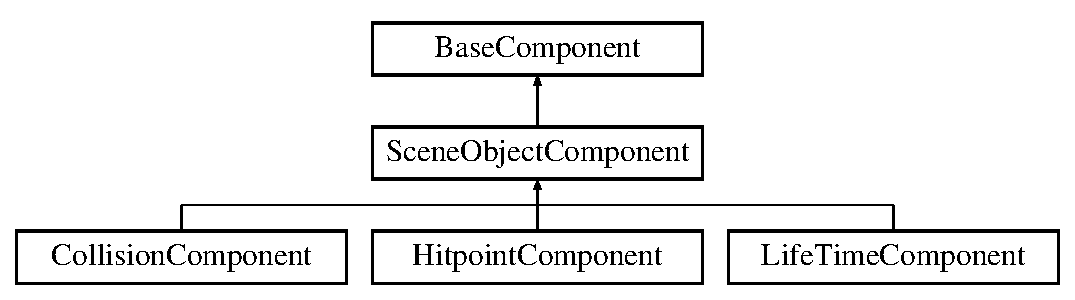
\includegraphics[height=3.000000cm]{class_base_component}
\end{center}
\end{figure}
\subsection*{Public Member Functions}
\begin{DoxyCompactItemize}
\item 
\hyperlink{class_base_component_ab5956c1e3164494e3bb46c65b5a3130a}{Base\+Component} (const std\+::string \&name)
\begin{DoxyCompactList}\small\item\em Default constructor. \end{DoxyCompactList}\item 
virtual \hyperlink{class_base_component_ab281730e838c4cb33e96ab6d6b7fe15f}{$\sim$\+Base\+Component} ()
\begin{DoxyCompactList}\small\item\em Default destructor. \end{DoxyCompactList}\item 
const std\+::string \& \hyperlink{class_base_component_a16c78063bc26ca947dc9944b370e9fdb}{get\+Name} () const 
\begin{DoxyCompactList}\small\item\em Access the identifying name of the component\textquotesingle{}s class. \end{DoxyCompactList}\end{DoxyCompactItemize}
\subsection*{Private Attributes}
\begin{DoxyCompactItemize}
\item 
const std\+::string \hyperlink{class_base_component_a45ae101f5812bec0b034a22283e91109}{m\+\_\+\+Name}
\begin{DoxyCompactList}\small\item\em Identifying name of the component class. \end{DoxyCompactList}\end{DoxyCompactItemize}


\subsection{Detailed Description}
Abstract base class for deriving components from. 

\begin{DoxyAuthor}{Author}
Hayley Hatton 
\end{DoxyAuthor}
\begin{DoxyDate}{Date}
06/03/2016 
\end{DoxyDate}


Definition at line 11 of file Base\+Component.\+h.



\subsection{Constructor \& Destructor Documentation}
\index{Base\+Component@{Base\+Component}!Base\+Component@{Base\+Component}}
\index{Base\+Component@{Base\+Component}!Base\+Component@{Base\+Component}}
\subsubsection[{\texorpdfstring{Base\+Component(const std\+::string \&name)}{BaseComponent(const std::string &name)}}]{\setlength{\rightskip}{0pt plus 5cm}Base\+Component\+::\+Base\+Component (
\begin{DoxyParamCaption}
\item[{const std\+::string \&}]{name}
\end{DoxyParamCaption}
)\hspace{0.3cm}{\ttfamily [inline]}}\hypertarget{class_base_component_ab5956c1e3164494e3bb46c65b5a3130a}{}\label{class_base_component_ab5956c1e3164494e3bb46c65b5a3130a}


Default constructor. 


\begin{DoxyParams}{Parameters}
{\em name} & Identifying name of the component class \\
\hline
\end{DoxyParams}


Definition at line 18 of file Base\+Component.\+h.

\index{Base\+Component@{Base\+Component}!````~Base\+Component@{$\sim$\+Base\+Component}}
\index{````~Base\+Component@{$\sim$\+Base\+Component}!Base\+Component@{Base\+Component}}
\subsubsection[{\texorpdfstring{$\sim$\+Base\+Component()}{~BaseComponent()}}]{\setlength{\rightskip}{0pt plus 5cm}virtual Base\+Component\+::$\sim$\+Base\+Component (
\begin{DoxyParamCaption}
{}
\end{DoxyParamCaption}
)\hspace{0.3cm}{\ttfamily [inline]}, {\ttfamily [virtual]}}\hypertarget{class_base_component_ab281730e838c4cb33e96ab6d6b7fe15f}{}\label{class_base_component_ab281730e838c4cb33e96ab6d6b7fe15f}


Default destructor. 



Definition at line 21 of file Base\+Component.\+h.



\subsection{Member Function Documentation}
\index{Base\+Component@{Base\+Component}!get\+Name@{get\+Name}}
\index{get\+Name@{get\+Name}!Base\+Component@{Base\+Component}}
\subsubsection[{\texorpdfstring{get\+Name() const }{getName() const }}]{\setlength{\rightskip}{0pt plus 5cm}const std\+::string\& Base\+Component\+::get\+Name (
\begin{DoxyParamCaption}
{}
\end{DoxyParamCaption}
) const\hspace{0.3cm}{\ttfamily [inline]}}\hypertarget{class_base_component_a16c78063bc26ca947dc9944b370e9fdb}{}\label{class_base_component_a16c78063bc26ca947dc9944b370e9fdb}


Access the identifying name of the component\textquotesingle{}s class. 

\begin{DoxyReturn}{Returns}
Identifying name of the component class 
\end{DoxyReturn}


Definition at line 28 of file Base\+Component.\+h.



References m\+\_\+\+Name.



\subsection{Member Data Documentation}
\index{Base\+Component@{Base\+Component}!m\+\_\+\+Name@{m\+\_\+\+Name}}
\index{m\+\_\+\+Name@{m\+\_\+\+Name}!Base\+Component@{Base\+Component}}
\subsubsection[{\texorpdfstring{m\+\_\+\+Name}{m_Name}}]{\setlength{\rightskip}{0pt plus 5cm}const std\+::string Base\+Component\+::m\+\_\+\+Name\hspace{0.3cm}{\ttfamily [private]}}\hypertarget{class_base_component_a45ae101f5812bec0b034a22283e91109}{}\label{class_base_component_a45ae101f5812bec0b034a22283e91109}


Identifying name of the component class. 



Definition at line 31 of file Base\+Component.\+h.



Referenced by get\+Name().



The documentation for this class was generated from the following file\+:\begin{DoxyCompactItemize}
\item 
Lunar\+Drift/engine/components/\hyperlink{_base_component_8h}{Base\+Component.\+h}\end{DoxyCompactItemize}

\hypertarget{class_button_down_event}{}\section{Button\+Down\+Event Class Reference}
\label{class_button_down_event}\index{Button\+Down\+Event@{Button\+Down\+Event}}


{\ttfamily \#include $<$Button\+Down\+Event.\+h$>$}

Inheritance diagram for Button\+Down\+Event\+:\begin{figure}[H]
\begin{center}
\leavevmode
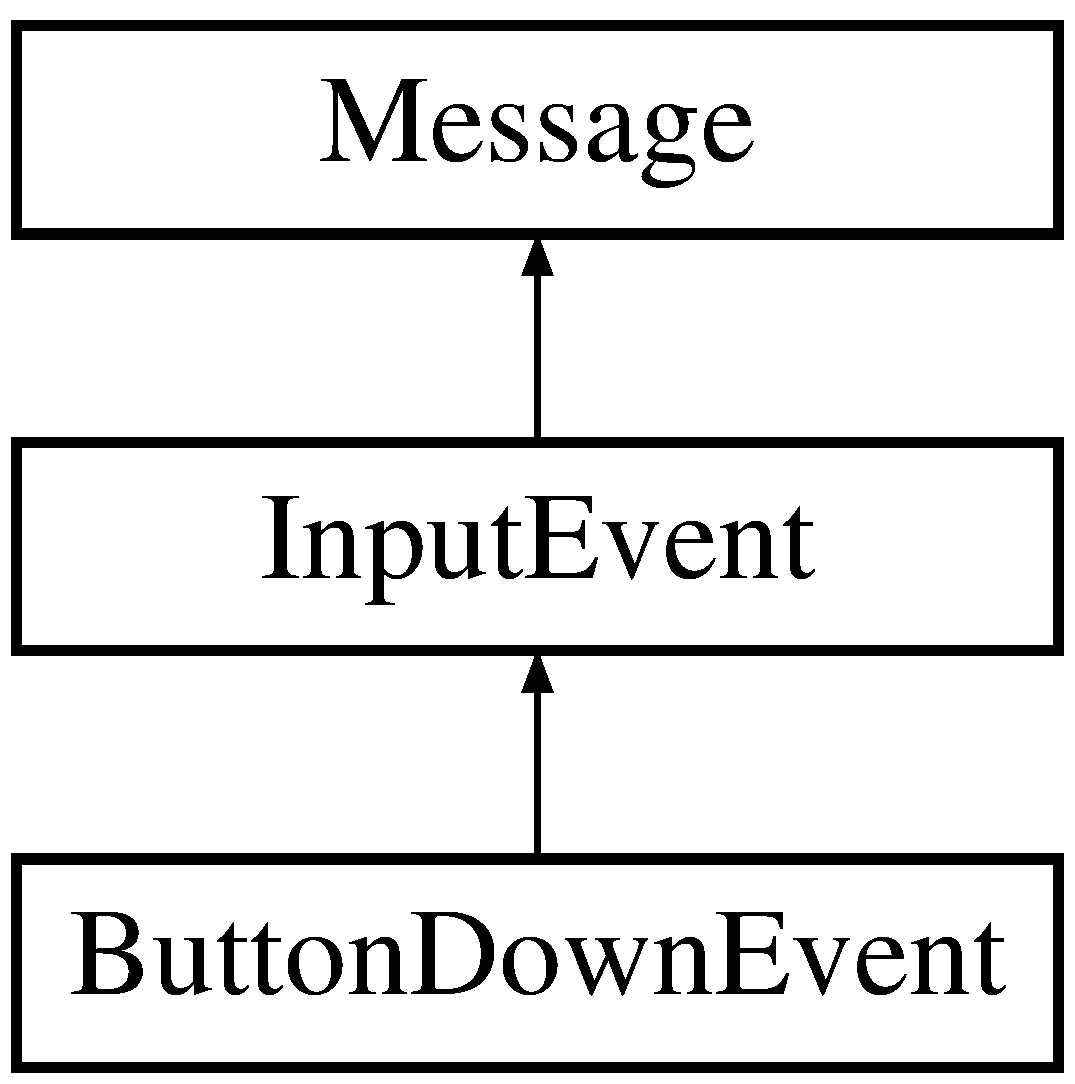
\includegraphics[height=3.000000cm]{class_button_down_event}
\end{center}
\end{figure}
\subsection*{Public Member Functions}
\begin{DoxyCompactItemize}
\item 
\hyperlink{class_button_down_event_ada6dbeac39500334c9e5c62503b41c8f}{Button\+Down\+Event} (const std\+::string \&input\+Name)
\item 
virtual \hyperlink{class_button_down_event_a61d89663686845499cc361d33beb1179}{$\sim$\+Button\+Down\+Event} ()
\item 
const std\+::string \& \hyperlink{class_button_down_event_a9c70a3a61c0721eaeb926156276efaa6}{get\+Input\+Name} () const 
\end{DoxyCompactItemize}
\subsection*{Private Attributes}
\begin{DoxyCompactItemize}
\item 
const std\+::string \hyperlink{class_button_down_event_a2880f23f03f0360a60481e3ebe974391}{m\+\_\+\+Input\+Name}
\begin{DoxyCompactList}\small\item\em Mapped name of the associated input btn. \end{DoxyCompactList}\end{DoxyCompactItemize}


\subsection{Detailed Description}


Definition at line 5 of file Button\+Down\+Event.\+h.



\subsection{Constructor \& Destructor Documentation}
\index{Button\+Down\+Event@{Button\+Down\+Event}!Button\+Down\+Event@{Button\+Down\+Event}}
\index{Button\+Down\+Event@{Button\+Down\+Event}!Button\+Down\+Event@{Button\+Down\+Event}}
\subsubsection[{\texorpdfstring{Button\+Down\+Event(const std\+::string \&input\+Name)}{ButtonDownEvent(const std::string &inputName)}}]{\setlength{\rightskip}{0pt plus 5cm}Button\+Down\+Event\+::\+Button\+Down\+Event (
\begin{DoxyParamCaption}
\item[{const std\+::string \&}]{input\+Name}
\end{DoxyParamCaption}
)}\hypertarget{class_button_down_event_ada6dbeac39500334c9e5c62503b41c8f}{}\label{class_button_down_event_ada6dbeac39500334c9e5c62503b41c8f}
Default constructor 

Definition at line 3 of file Button\+Down\+Event.\+cpp.

\index{Button\+Down\+Event@{Button\+Down\+Event}!````~Button\+Down\+Event@{$\sim$\+Button\+Down\+Event}}
\index{````~Button\+Down\+Event@{$\sim$\+Button\+Down\+Event}!Button\+Down\+Event@{Button\+Down\+Event}}
\subsubsection[{\texorpdfstring{$\sim$\+Button\+Down\+Event()}{~ButtonDownEvent()}}]{\setlength{\rightskip}{0pt plus 5cm}Button\+Down\+Event\+::$\sim$\+Button\+Down\+Event (
\begin{DoxyParamCaption}
{}
\end{DoxyParamCaption}
)\hspace{0.3cm}{\ttfamily [virtual]}}\hypertarget{class_button_down_event_a61d89663686845499cc361d33beb1179}{}\label{class_button_down_event_a61d89663686845499cc361d33beb1179}
Default destructor 

Definition at line 10 of file Button\+Down\+Event.\+cpp.



\subsection{Member Function Documentation}
\index{Button\+Down\+Event@{Button\+Down\+Event}!get\+Input\+Name@{get\+Input\+Name}}
\index{get\+Input\+Name@{get\+Input\+Name}!Button\+Down\+Event@{Button\+Down\+Event}}
\subsubsection[{\texorpdfstring{get\+Input\+Name() const }{getInputName() const }}]{\setlength{\rightskip}{0pt plus 5cm}const std\+::string\& Button\+Down\+Event\+::get\+Input\+Name (
\begin{DoxyParamCaption}
{}
\end{DoxyParamCaption}
) const\hspace{0.3cm}{\ttfamily [inline]}}\hypertarget{class_button_down_event_a9c70a3a61c0721eaeb926156276efaa6}{}\label{class_button_down_event_a9c70a3a61c0721eaeb926156276efaa6}


Definition at line 15 of file Button\+Down\+Event.\+h.



References m\+\_\+\+Input\+Name.



\subsection{Member Data Documentation}
\index{Button\+Down\+Event@{Button\+Down\+Event}!m\+\_\+\+Input\+Name@{m\+\_\+\+Input\+Name}}
\index{m\+\_\+\+Input\+Name@{m\+\_\+\+Input\+Name}!Button\+Down\+Event@{Button\+Down\+Event}}
\subsubsection[{\texorpdfstring{m\+\_\+\+Input\+Name}{m_InputName}}]{\setlength{\rightskip}{0pt plus 5cm}const std\+::string Button\+Down\+Event\+::m\+\_\+\+Input\+Name\hspace{0.3cm}{\ttfamily [private]}}\hypertarget{class_button_down_event_a2880f23f03f0360a60481e3ebe974391}{}\label{class_button_down_event_a2880f23f03f0360a60481e3ebe974391}


Mapped name of the associated input btn. 



Definition at line 20 of file Button\+Down\+Event.\+h.



Referenced by get\+Input\+Name().



The documentation for this class was generated from the following files\+:\begin{DoxyCompactItemize}
\item 
Lunar\+Drift/engine/comms/predefined/\hyperlink{_button_down_event_8h}{Button\+Down\+Event.\+h}\item 
Lunar\+Drift/engine/comms/predefined/\hyperlink{_button_down_event_8cpp}{Button\+Down\+Event.\+cpp}\end{DoxyCompactItemize}

\hypertarget{class_button_up_event}{}\section{Button\+Up\+Event Class Reference}
\label{class_button_up_event}\index{Button\+Up\+Event@{Button\+Up\+Event}}


{\ttfamily \#include $<$Button\+Up\+Event.\+h$>$}

Inheritance diagram for Button\+Up\+Event\+:\begin{figure}[H]
\begin{center}
\leavevmode
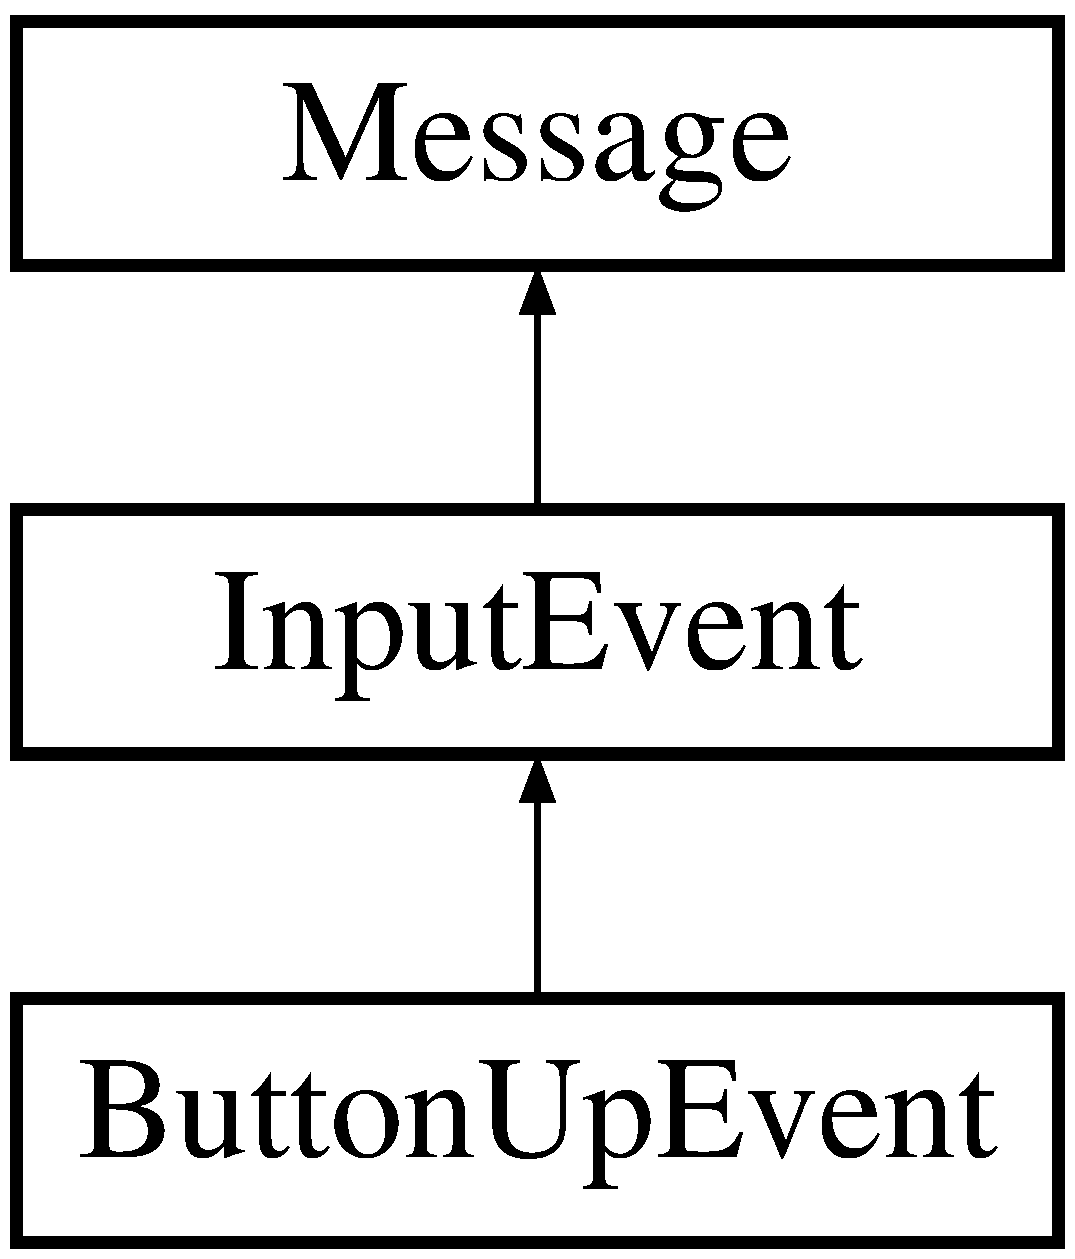
\includegraphics[height=3.000000cm]{class_button_up_event}
\end{center}
\end{figure}
\subsection*{Public Member Functions}
\begin{DoxyCompactItemize}
\item 
\hyperlink{class_button_up_event_a4f17bfe1bc01e5f260e1fb98c50702d8}{Button\+Up\+Event} (const std\+::string \&input\+Name)
\item 
virtual \hyperlink{class_button_up_event_a3d60db80c7d6124f4281c045851f75e0}{$\sim$\+Button\+Up\+Event} ()
\item 
const std\+::string \& \hyperlink{class_button_up_event_a7e34b2f7f1d3e5f05abfe6487ec74137}{get\+Input\+Name} () const 
\end{DoxyCompactItemize}
\subsection*{Private Attributes}
\begin{DoxyCompactItemize}
\item 
const std\+::string \hyperlink{class_button_up_event_a10fa86bad63b034f0d68e11dd5233f22}{m\+\_\+\+Input\+Name}
\begin{DoxyCompactList}\small\item\em Mapped name of the associated input btn. \end{DoxyCompactList}\end{DoxyCompactItemize}


\subsection{Detailed Description}


Definition at line 6 of file Button\+Up\+Event.\+h.



\subsection{Constructor \& Destructor Documentation}
\index{Button\+Up\+Event@{Button\+Up\+Event}!Button\+Up\+Event@{Button\+Up\+Event}}
\index{Button\+Up\+Event@{Button\+Up\+Event}!Button\+Up\+Event@{Button\+Up\+Event}}
\subsubsection[{\texorpdfstring{Button\+Up\+Event(const std\+::string \&input\+Name)}{ButtonUpEvent(const std::string &inputName)}}]{\setlength{\rightskip}{0pt plus 5cm}Button\+Up\+Event\+::\+Button\+Up\+Event (
\begin{DoxyParamCaption}
\item[{const std\+::string \&}]{input\+Name}
\end{DoxyParamCaption}
)}\hypertarget{class_button_up_event_a4f17bfe1bc01e5f260e1fb98c50702d8}{}\label{class_button_up_event_a4f17bfe1bc01e5f260e1fb98c50702d8}
Default constructor 

Definition at line 3 of file Button\+Up\+Event.\+cpp.

\index{Button\+Up\+Event@{Button\+Up\+Event}!````~Button\+Up\+Event@{$\sim$\+Button\+Up\+Event}}
\index{````~Button\+Up\+Event@{$\sim$\+Button\+Up\+Event}!Button\+Up\+Event@{Button\+Up\+Event}}
\subsubsection[{\texorpdfstring{$\sim$\+Button\+Up\+Event()}{~ButtonUpEvent()}}]{\setlength{\rightskip}{0pt plus 5cm}Button\+Up\+Event\+::$\sim$\+Button\+Up\+Event (
\begin{DoxyParamCaption}
{}
\end{DoxyParamCaption}
)\hspace{0.3cm}{\ttfamily [virtual]}}\hypertarget{class_button_up_event_a3d60db80c7d6124f4281c045851f75e0}{}\label{class_button_up_event_a3d60db80c7d6124f4281c045851f75e0}
Default destructor 

Definition at line 10 of file Button\+Up\+Event.\+cpp.



\subsection{Member Function Documentation}
\index{Button\+Up\+Event@{Button\+Up\+Event}!get\+Input\+Name@{get\+Input\+Name}}
\index{get\+Input\+Name@{get\+Input\+Name}!Button\+Up\+Event@{Button\+Up\+Event}}
\subsubsection[{\texorpdfstring{get\+Input\+Name() const }{getInputName() const }}]{\setlength{\rightskip}{0pt plus 5cm}const std\+::string\& Button\+Up\+Event\+::get\+Input\+Name (
\begin{DoxyParamCaption}
{}
\end{DoxyParamCaption}
) const\hspace{0.3cm}{\ttfamily [inline]}}\hypertarget{class_button_up_event_a7e34b2f7f1d3e5f05abfe6487ec74137}{}\label{class_button_up_event_a7e34b2f7f1d3e5f05abfe6487ec74137}


Definition at line 16 of file Button\+Up\+Event.\+h.



References m\+\_\+\+Input\+Name.



\subsection{Member Data Documentation}
\index{Button\+Up\+Event@{Button\+Up\+Event}!m\+\_\+\+Input\+Name@{m\+\_\+\+Input\+Name}}
\index{m\+\_\+\+Input\+Name@{m\+\_\+\+Input\+Name}!Button\+Up\+Event@{Button\+Up\+Event}}
\subsubsection[{\texorpdfstring{m\+\_\+\+Input\+Name}{m_InputName}}]{\setlength{\rightskip}{0pt plus 5cm}const std\+::string Button\+Up\+Event\+::m\+\_\+\+Input\+Name\hspace{0.3cm}{\ttfamily [private]}}\hypertarget{class_button_up_event_a10fa86bad63b034f0d68e11dd5233f22}{}\label{class_button_up_event_a10fa86bad63b034f0d68e11dd5233f22}


Mapped name of the associated input btn. 



Definition at line 21 of file Button\+Up\+Event.\+h.



Referenced by get\+Input\+Name().



The documentation for this class was generated from the following files\+:\begin{DoxyCompactItemize}
\item 
Lunar\+Drift/engine/comms/predefined/\hyperlink{_button_up_event_8h}{Button\+Up\+Event.\+h}\item 
Lunar\+Drift/engine/comms/predefined/\hyperlink{_button_up_event_8cpp}{Button\+Up\+Event.\+cpp}\end{DoxyCompactItemize}

\hypertarget{class_camera}{}\section{Camera Class Reference}
\label{class_camera}\index{Camera@{Camera}}


Describes a camera for viewing a scene.  




{\ttfamily \#include $<$Camera.\+h$>$}

\subsection*{Public Member Functions}
\begin{DoxyCompactItemize}
\item 
\hyperlink{class_camera_ac817e3c9d822bca54936a3bc70245137}{Camera} (G\+Luint width, G\+Luint height, G\+Lfloat nearZ, G\+Lfloat farZ)
\begin{DoxyCompactList}\small\item\em Create a camera with an orthogonal lens. \end{DoxyCompactList}\item 
\hyperlink{class_camera_a25980407bbf15173f5dbcf34260ac841}{Camera} (G\+Luint width, G\+Luint height, G\+Lfloat nearZ, G\+Lfloat farZ, G\+Lfloat fovy)
\begin{DoxyCompactList}\small\item\em Create a camera with a perspective lens. \end{DoxyCompactList}\item 
virtual \hyperlink{class_camera_ad1897942d0ccf91052386388a497349f}{$\sim$\+Camera} ()
\begin{DoxyCompactList}\small\item\em Default destructor. \end{DoxyCompactList}\item 
void \hyperlink{class_camera_a163d38c1b0f1690a55e677cf7861b457}{set\+Orthogonal} (G\+Luint width, G\+Luint height, G\+Lfloat nearZ, G\+Lfloat farZ)
\begin{DoxyCompactList}\small\item\em Set an orthogonal lens for the camera. \end{DoxyCompactList}\item 
void \hyperlink{class_camera_a2488706c1ca5e9c4bc92dfef65c91aae}{set\+Perspective} (G\+Luint width, G\+Luint height, G\+Lfloat nearZ, G\+Lfloat farZ, G\+Lfloat fovy)
\begin{DoxyCompactList}\small\item\em Set a perspective lens for the camera. \end{DoxyCompactList}\item 
void \hyperlink{class_camera_af04cfb4727b7b20e4728e0cdebf8e1c9}{look\+At} (const glm\+::vec3 \&eye, const glm\+::vec3 \&focus, const glm\+::vec3 \&up)
\begin{DoxyCompactList}\small\item\em Set the camera in the scene using classic \char`\"{}look-\/at\char`\"{} descriptors. \end{DoxyCompactList}\item 
void \hyperlink{class_camera_a84aef2b61721b9246414a89a09fac235}{pan} (const glm\+::vec3 \&dp)
\begin{DoxyCompactList}\small\item\em Pan the camera. \end{DoxyCompactList}\item 
void \hyperlink{class_camera_add2cd15792f3a290a56311334d736898}{rotateX} (G\+Lfloat theta)
\begin{DoxyCompactList}\small\item\em Rotate through the Y-\/Z plane (\char`\"{}\+X-\/axis\char`\"{}/\char`\"{}pitch\char`\"{}) \end{DoxyCompactList}\item 
void \hyperlink{class_camera_ae2354566eb8c0420537b3f61350a8c6f}{rotateY} (G\+Lfloat theta)
\begin{DoxyCompactList}\small\item\em Rotate through the X-\/Z plane (\char`\"{}\+Y-\/axis\char`\"{}/\char`\"{}yaw\char`\"{}) \end{DoxyCompactList}\item 
void \hyperlink{class_camera_a83b1b32ad7a7746a91ab855c160b6c19}{rotateZ} (G\+Lfloat theta)
\begin{DoxyCompactList}\small\item\em Rotate through the X-\/Y plane (\char`\"{}\+Z-\/axis\char`\"{}/\char`\"{}roll\char`\"{}) \end{DoxyCompactList}\item 
const glm\+::vec3 \& \hyperlink{class_camera_ac3f20f73b8e37f445da786bfe9e33690}{get\+Position} () const 
\begin{DoxyCompactList}\small\item\em Access the position of the camera. \end{DoxyCompactList}\item 
const glm\+::mat4 \& \hyperlink{class_camera_a8770289592db9df6f7ab08de42d6fa9c}{get\+View\+Matrix} () const 
\begin{DoxyCompactList}\small\item\em Access the current view matrix state. \end{DoxyCompactList}\item 
const glm\+::mat4 \& \hyperlink{class_camera_a02898d27ba55e88b3bed38d41be55215}{get\+Projection\+Matrix} () const 
\begin{DoxyCompactList}\small\item\em Access the current projection matrix state. \end{DoxyCompactList}\item 
void \hyperlink{class_camera_a390070b89f45af162d48fca2e70ea299}{apply} (\hyperlink{class_context}{Context} $\ast$context, \hyperlink{class_shader_program}{Shader\+Program} $\ast$shader) const 
\begin{DoxyCompactList}\small\item\em Upload the camera matrices to a given shader program\textquotesingle{}s uniforms. \end{DoxyCompactList}\item 
void \hyperlink{class_camera_a05a6d1c771d22375d60cdf249fbb2492}{apply} (\hyperlink{class_context}{Context} $\ast$context, \hyperlink{class_shader_uniform_block}{Shader\+Uniform\+Block} $\ast$buffer) const 
\begin{DoxyCompactList}\small\item\em Upload the camera matrices to a uniform buffer across all shaders. \end{DoxyCompactList}\end{DoxyCompactItemize}
\subsection*{Private Attributes}
\begin{DoxyCompactItemize}
\item 
glm\+::mat4 \hyperlink{class_camera_a678ced6db61f473f65734c8a1522ea80}{m\+\_\+\+View\+Matrix}
\begin{DoxyCompactList}\small\item\em Current view matrix state. \end{DoxyCompactList}\item 
glm\+::mat4 \hyperlink{class_camera_a60d7a52ef114cb65fd2a079deceb5ccf}{m\+\_\+\+Proj\+Matrix}
\begin{DoxyCompactList}\small\item\em Current projection matrix state. \end{DoxyCompactList}\end{DoxyCompactItemize}


\subsection{Detailed Description}
Describes a camera for viewing a scene. 

\begin{DoxyAuthor}{Author}
Hayley Hatton 
\end{DoxyAuthor}
\begin{DoxyDate}{Date}
07/03/2016 
\end{DoxyDate}


Definition at line 13 of file Camera.\+h.



\subsection{Constructor \& Destructor Documentation}
\index{Camera@{Camera}!Camera@{Camera}}
\index{Camera@{Camera}!Camera@{Camera}}
\subsubsection[{\texorpdfstring{Camera(\+G\+Luint width, G\+Luint height, G\+Lfloat near\+Z, G\+Lfloat far\+Z)}{Camera(GLuint width, GLuint height, GLfloat nearZ, GLfloat farZ)}}]{\setlength{\rightskip}{0pt plus 5cm}Camera\+::\+Camera (
\begin{DoxyParamCaption}
\item[{G\+Luint}]{width, }
\item[{G\+Luint}]{height, }
\item[{G\+Lfloat}]{nearZ, }
\item[{G\+Lfloat}]{farZ}
\end{DoxyParamCaption}
)}\hypertarget{class_camera_ac817e3c9d822bca54936a3bc70245137}{}\label{class_camera_ac817e3c9d822bca54936a3bc70245137}


Create a camera with an orthogonal lens. 


\begin{DoxyParams}{Parameters}
{\em width} & Width of the viewport \\
\hline
{\em height} & Height of the viewport \\
\hline
{\em nearZ} & Near-\/plane Z coordinate \\
\hline
{\em farZ} & Far-\/plane Z coordinate \\
\hline
\end{DoxyParams}


Definition at line 5 of file Camera.\+cpp.



References set\+Orthogonal().

\index{Camera@{Camera}!Camera@{Camera}}
\index{Camera@{Camera}!Camera@{Camera}}
\subsubsection[{\texorpdfstring{Camera(\+G\+Luint width, G\+Luint height, G\+Lfloat near\+Z, G\+Lfloat far\+Z, G\+Lfloat fovy)}{Camera(GLuint width, GLuint height, GLfloat nearZ, GLfloat farZ, GLfloat fovy)}}]{\setlength{\rightskip}{0pt plus 5cm}Camera\+::\+Camera (
\begin{DoxyParamCaption}
\item[{G\+Luint}]{width, }
\item[{G\+Luint}]{height, }
\item[{G\+Lfloat}]{nearZ, }
\item[{G\+Lfloat}]{farZ, }
\item[{G\+Lfloat}]{fovy}
\end{DoxyParamCaption}
)}\hypertarget{class_camera_a25980407bbf15173f5dbcf34260ac841}{}\label{class_camera_a25980407bbf15173f5dbcf34260ac841}


Create a camera with a perspective lens. 


\begin{DoxyParams}{Parameters}
{\em width} & Width of the viewport \\
\hline
{\em height} & Height of the viewport \\
\hline
{\em nearZ} & Near-\/plane Z coordinate \\
\hline
{\em farZ} & Far-\/plane Z coordinate \\
\hline
{\em fovy} & Field-\/of-\/view, in degrees \\
\hline
\end{DoxyParams}


Definition at line 12 of file Camera.\+cpp.



References set\+Perspective().

\index{Camera@{Camera}!````~Camera@{$\sim$\+Camera}}
\index{````~Camera@{$\sim$\+Camera}!Camera@{Camera}}
\subsubsection[{\texorpdfstring{$\sim$\+Camera()}{~Camera()}}]{\setlength{\rightskip}{0pt plus 5cm}Camera\+::$\sim$\+Camera (
\begin{DoxyParamCaption}
{}
\end{DoxyParamCaption}
)\hspace{0.3cm}{\ttfamily [virtual]}}\hypertarget{class_camera_ad1897942d0ccf91052386388a497349f}{}\label{class_camera_ad1897942d0ccf91052386388a497349f}


Default destructor. 



Definition at line 20 of file Camera.\+cpp.



\subsection{Member Function Documentation}
\index{Camera@{Camera}!apply@{apply}}
\index{apply@{apply}!Camera@{Camera}}
\subsubsection[{\texorpdfstring{apply(\+Context $\ast$context, Shader\+Program $\ast$shader) const }{apply(Context *context, ShaderProgram *shader) const }}]{\setlength{\rightskip}{0pt plus 5cm}void Camera\+::apply (
\begin{DoxyParamCaption}
\item[{{\bf Context} $\ast$}]{context, }
\item[{{\bf Shader\+Program} $\ast$}]{shader}
\end{DoxyParamCaption}
) const}\hypertarget{class_camera_a390070b89f45af162d48fca2e70ea299}{}\label{class_camera_a390070b89f45af162d48fca2e70ea299}


Upload the camera matrices to a given shader program\textquotesingle{}s uniforms. 


\begin{DoxyParams}{Parameters}
{\em context} & Graphics context \\
\hline
{\em shader} & Ptr to the shader program to upload matrices to \\
\hline
\end{DoxyParams}


Definition at line 76 of file Camera.\+cpp.



References Shader\+Program\+::get\+Uniform\+Location(), m\+\_\+\+Proj\+Matrix, m\+\_\+\+View\+Matrix, and Shader\+Program\+::use().



Referenced by get\+Projection\+Matrix().

\index{Camera@{Camera}!apply@{apply}}
\index{apply@{apply}!Camera@{Camera}}
\subsubsection[{\texorpdfstring{apply(\+Context $\ast$context, Shader\+Uniform\+Block $\ast$buffer) const }{apply(Context *context, ShaderUniformBlock *buffer) const }}]{\setlength{\rightskip}{0pt plus 5cm}void Camera\+::apply (
\begin{DoxyParamCaption}
\item[{{\bf Context} $\ast$}]{context, }
\item[{{\bf Shader\+Uniform\+Block} $\ast$}]{buffer}
\end{DoxyParamCaption}
) const}\hypertarget{class_camera_a05a6d1c771d22375d60cdf249fbb2492}{}\label{class_camera_a05a6d1c771d22375d60cdf249fbb2492}


Upload the camera matrices to a uniform buffer across all shaders. 


\begin{DoxyParams}{Parameters}
{\em context} & Graphics context \\
\hline
{\em shader} & Ptr to the uniform buffer to upload matrices to \\
\hline
\end{DoxyParams}
\begin{DoxyRefDesc}{Todo}
\item[\hyperlink{todo__todo000009}{Todo}](Hayley\#6\#03/08/16)\+: Uploading of camera state to shader uniform blocks \end{DoxyRefDesc}


Definition at line 95 of file Camera.\+cpp.

\index{Camera@{Camera}!get\+Position@{get\+Position}}
\index{get\+Position@{get\+Position}!Camera@{Camera}}
\subsubsection[{\texorpdfstring{get\+Position() const }{getPosition() const }}]{\setlength{\rightskip}{0pt plus 5cm}const glm\+::vec3\& Camera\+::get\+Position (
\begin{DoxyParamCaption}
{}
\end{DoxyParamCaption}
) const}\hypertarget{class_camera_ac3f20f73b8e37f445da786bfe9e33690}{}\label{class_camera_ac3f20f73b8e37f445da786bfe9e33690}


Access the position of the camera. 

\begin{DoxyReturn}{Returns}
3-\/component vector of the position in space 
\end{DoxyReturn}
\index{Camera@{Camera}!get\+Projection\+Matrix@{get\+Projection\+Matrix}}
\index{get\+Projection\+Matrix@{get\+Projection\+Matrix}!Camera@{Camera}}
\subsubsection[{\texorpdfstring{get\+Projection\+Matrix() const }{getProjectionMatrix() const }}]{\setlength{\rightskip}{0pt plus 5cm}const glm\+::mat4\& Camera\+::get\+Projection\+Matrix (
\begin{DoxyParamCaption}
{}
\end{DoxyParamCaption}
) const\hspace{0.3cm}{\ttfamily [inline]}}\hypertarget{class_camera_a02898d27ba55e88b3bed38d41be55215}{}\label{class_camera_a02898d27ba55e88b3bed38d41be55215}


Access the current projection matrix state. 

\begin{DoxyReturn}{Returns}
Projection matrix (4x4) 
\end{DoxyReturn}


Definition at line 117 of file Camera.\+h.



References apply(), and m\+\_\+\+Proj\+Matrix.

\index{Camera@{Camera}!get\+View\+Matrix@{get\+View\+Matrix}}
\index{get\+View\+Matrix@{get\+View\+Matrix}!Camera@{Camera}}
\subsubsection[{\texorpdfstring{get\+View\+Matrix() const }{getViewMatrix() const }}]{\setlength{\rightskip}{0pt plus 5cm}const glm\+::mat4\& Camera\+::get\+View\+Matrix (
\begin{DoxyParamCaption}
{}
\end{DoxyParamCaption}
) const\hspace{0.3cm}{\ttfamily [inline]}}\hypertarget{class_camera_a8770289592db9df6f7ab08de42d6fa9c}{}\label{class_camera_a8770289592db9df6f7ab08de42d6fa9c}


Access the current view matrix state. 

\begin{DoxyReturn}{Returns}
View matrix (4x4) 
\end{DoxyReturn}


Definition at line 111 of file Camera.\+h.



References m\+\_\+\+View\+Matrix.

\index{Camera@{Camera}!look\+At@{look\+At}}
\index{look\+At@{look\+At}!Camera@{Camera}}
\subsubsection[{\texorpdfstring{look\+At(const glm\+::vec3 \&eye, const glm\+::vec3 \&focus, const glm\+::vec3 \&up)}{lookAt(const glm::vec3 &eye, const glm::vec3 &focus, const glm::vec3 &up)}}]{\setlength{\rightskip}{0pt plus 5cm}void Camera\+::look\+At (
\begin{DoxyParamCaption}
\item[{const glm\+::vec3 \&}]{eye, }
\item[{const glm\+::vec3 \&}]{focus, }
\item[{const glm\+::vec3 \&}]{up}
\end{DoxyParamCaption}
)}\hypertarget{class_camera_af04cfb4727b7b20e4728e0cdebf8e1c9}{}\label{class_camera_af04cfb4727b7b20e4728e0cdebf8e1c9}


Set the camera in the scene using classic \char`\"{}look-\/at\char`\"{} descriptors. 


\begin{DoxyParams}{Parameters}
{\em eye} & Position of the camera in the scene \\
\hline
{\em focus} & Where the camera is looking at in the scene \\
\hline
{\em up} & Up-\/vector defining the orientation of the camera \\
\hline
\end{DoxyParams}


Definition at line 48 of file Camera.\+cpp.



References m\+\_\+\+View\+Matrix.

\index{Camera@{Camera}!pan@{pan}}
\index{pan@{pan}!Camera@{Camera}}
\subsubsection[{\texorpdfstring{pan(const glm\+::vec3 \&dp)}{pan(const glm::vec3 &dp)}}]{\setlength{\rightskip}{0pt plus 5cm}void Camera\+::pan (
\begin{DoxyParamCaption}
\item[{const glm\+::vec3 \&}]{dp}
\end{DoxyParamCaption}
)}\hypertarget{class_camera_a84aef2b61721b9246414a89a09fac235}{}\label{class_camera_a84aef2b61721b9246414a89a09fac235}


Pan the camera. 


\begin{DoxyParams}{Parameters}
{\em dp} & Delta-\/position \\
\hline
\end{DoxyParams}


Definition at line 56 of file Camera.\+cpp.



References m\+\_\+\+View\+Matrix.

\index{Camera@{Camera}!rotateX@{rotateX}}
\index{rotateX@{rotateX}!Camera@{Camera}}
\subsubsection[{\texorpdfstring{rotate\+X(\+G\+Lfloat theta)}{rotateX(GLfloat theta)}}]{\setlength{\rightskip}{0pt plus 5cm}void Camera\+::rotateX (
\begin{DoxyParamCaption}
\item[{G\+Lfloat}]{theta}
\end{DoxyParamCaption}
)}\hypertarget{class_camera_add2cd15792f3a290a56311334d736898}{}\label{class_camera_add2cd15792f3a290a56311334d736898}


Rotate through the Y-\/Z plane (\char`\"{}\+X-\/axis\char`\"{}/\char`\"{}pitch\char`\"{}) 


\begin{DoxyParams}{Parameters}
{\em theta} & Angle in degrees through which to rotate the camera \\
\hline
\end{DoxyParams}


Definition at line 61 of file Camera.\+cpp.



References f, and m\+\_\+\+View\+Matrix.

\index{Camera@{Camera}!rotateY@{rotateY}}
\index{rotateY@{rotateY}!Camera@{Camera}}
\subsubsection[{\texorpdfstring{rotate\+Y(\+G\+Lfloat theta)}{rotateY(GLfloat theta)}}]{\setlength{\rightskip}{0pt plus 5cm}void Camera\+::rotateY (
\begin{DoxyParamCaption}
\item[{G\+Lfloat}]{theta}
\end{DoxyParamCaption}
)}\hypertarget{class_camera_ae2354566eb8c0420537b3f61350a8c6f}{}\label{class_camera_ae2354566eb8c0420537b3f61350a8c6f}


Rotate through the X-\/Z plane (\char`\"{}\+Y-\/axis\char`\"{}/\char`\"{}yaw\char`\"{}) 


\begin{DoxyParams}{Parameters}
{\em theta} & Angle in degrees through which to rotate the camera \\
\hline
\end{DoxyParams}


Definition at line 66 of file Camera.\+cpp.



References f, and m\+\_\+\+View\+Matrix.

\index{Camera@{Camera}!rotateZ@{rotateZ}}
\index{rotateZ@{rotateZ}!Camera@{Camera}}
\subsubsection[{\texorpdfstring{rotate\+Z(\+G\+Lfloat theta)}{rotateZ(GLfloat theta)}}]{\setlength{\rightskip}{0pt plus 5cm}void Camera\+::rotateZ (
\begin{DoxyParamCaption}
\item[{G\+Lfloat}]{theta}
\end{DoxyParamCaption}
)}\hypertarget{class_camera_a83b1b32ad7a7746a91ab855c160b6c19}{}\label{class_camera_a83b1b32ad7a7746a91ab855c160b6c19}


Rotate through the X-\/Y plane (\char`\"{}\+Z-\/axis\char`\"{}/\char`\"{}roll\char`\"{}) 


\begin{DoxyParams}{Parameters}
{\em theta} & Angle in degrees through which to rotate the camera \\
\hline
\end{DoxyParams}


Definition at line 71 of file Camera.\+cpp.



References f, and m\+\_\+\+View\+Matrix.

\index{Camera@{Camera}!set\+Orthogonal@{set\+Orthogonal}}
\index{set\+Orthogonal@{set\+Orthogonal}!Camera@{Camera}}
\subsubsection[{\texorpdfstring{set\+Orthogonal(\+G\+Luint width, G\+Luint height, G\+Lfloat near\+Z, G\+Lfloat far\+Z)}{setOrthogonal(GLuint width, GLuint height, GLfloat nearZ, GLfloat farZ)}}]{\setlength{\rightskip}{0pt plus 5cm}void Camera\+::set\+Orthogonal (
\begin{DoxyParamCaption}
\item[{G\+Luint}]{width, }
\item[{G\+Luint}]{height, }
\item[{G\+Lfloat}]{nearZ, }
\item[{G\+Lfloat}]{farZ}
\end{DoxyParamCaption}
)}\hypertarget{class_camera_a163d38c1b0f1690a55e677cf7861b457}{}\label{class_camera_a163d38c1b0f1690a55e677cf7861b457}


Set an orthogonal lens for the camera. 


\begin{DoxyParams}{Parameters}
{\em width} & Width of the viewport \\
\hline
{\em height} & Height of the viewport \\
\hline
{\em nearZ} & Near-\/plane Z coordinate \\
\hline
{\em farZ} & Far-\/plane Z coordinate \\
\hline
\end{DoxyParams}


Definition at line 26 of file Camera.\+cpp.



References f, and m\+\_\+\+Proj\+Matrix.



Referenced by Camera().

\index{Camera@{Camera}!set\+Perspective@{set\+Perspective}}
\index{set\+Perspective@{set\+Perspective}!Camera@{Camera}}
\subsubsection[{\texorpdfstring{set\+Perspective(\+G\+Luint width, G\+Luint height, G\+Lfloat near\+Z, G\+Lfloat far\+Z, G\+Lfloat fovy)}{setPerspective(GLuint width, GLuint height, GLfloat nearZ, GLfloat farZ, GLfloat fovy)}}]{\setlength{\rightskip}{0pt plus 5cm}void Camera\+::set\+Perspective (
\begin{DoxyParamCaption}
\item[{G\+Luint}]{width, }
\item[{G\+Luint}]{height, }
\item[{G\+Lfloat}]{nearZ, }
\item[{G\+Lfloat}]{farZ, }
\item[{G\+Lfloat}]{fovy}
\end{DoxyParamCaption}
)}\hypertarget{class_camera_a2488706c1ca5e9c4bc92dfef65c91aae}{}\label{class_camera_a2488706c1ca5e9c4bc92dfef65c91aae}


Set a perspective lens for the camera. 


\begin{DoxyParams}{Parameters}
{\em width} & Width of the viewport \\
\hline
{\em height} & Height of the viewport \\
\hline
{\em nearZ} & Near-\/plane Z coordinate \\
\hline
{\em farZ} & Far-\/plane Z coordinate \\
\hline
{\em fovy} & Field-\/of-\/view, in degrees \\
\hline
\end{DoxyParams}


Definition at line 36 of file Camera.\+cpp.



References h, m\+\_\+\+Proj\+Matrix, and w.



Referenced by Camera().



\subsection{Member Data Documentation}
\index{Camera@{Camera}!m\+\_\+\+Proj\+Matrix@{m\+\_\+\+Proj\+Matrix}}
\index{m\+\_\+\+Proj\+Matrix@{m\+\_\+\+Proj\+Matrix}!Camera@{Camera}}
\subsubsection[{\texorpdfstring{m\+\_\+\+Proj\+Matrix}{m_ProjMatrix}}]{\setlength{\rightskip}{0pt plus 5cm}glm\+::mat4 Camera\+::m\+\_\+\+Proj\+Matrix\hspace{0.3cm}{\ttfamily [private]}}\hypertarget{class_camera_a60d7a52ef114cb65fd2a079deceb5ccf}{}\label{class_camera_a60d7a52ef114cb65fd2a079deceb5ccf}


Current projection matrix state. 



Definition at line 135 of file Camera.\+h.



Referenced by apply(), get\+Projection\+Matrix(), set\+Orthogonal(), and set\+Perspective().

\index{Camera@{Camera}!m\+\_\+\+View\+Matrix@{m\+\_\+\+View\+Matrix}}
\index{m\+\_\+\+View\+Matrix@{m\+\_\+\+View\+Matrix}!Camera@{Camera}}
\subsubsection[{\texorpdfstring{m\+\_\+\+View\+Matrix}{m_ViewMatrix}}]{\setlength{\rightskip}{0pt plus 5cm}glm\+::mat4 Camera\+::m\+\_\+\+View\+Matrix\hspace{0.3cm}{\ttfamily [private]}}\hypertarget{class_camera_a678ced6db61f473f65734c8a1522ea80}{}\label{class_camera_a678ced6db61f473f65734c8a1522ea80}


Current view matrix state. 



Definition at line 134 of file Camera.\+h.



Referenced by apply(), get\+View\+Matrix(), look\+At(), pan(), rotate\+X(), rotate\+Y(), and rotate\+Z().



The documentation for this class was generated from the following files\+:\begin{DoxyCompactItemize}
\item 
Lunar\+Drift/engine/graphics/\hyperlink{_camera_8h}{Camera.\+h}\item 
Lunar\+Drift/engine/graphics/\hyperlink{_camera_8cpp}{Camera.\+cpp}\end{DoxyCompactItemize}

\hypertarget{class_collision_component}{}\section{Collision\+Component Class Reference}
\label{class_collision_component}\index{Collision\+Component@{Collision\+Component}}


Component that describes collision information about the parent.  




{\ttfamily \#include $<$Collision\+Component.\+h$>$}

Inheritance diagram for Collision\+Component\+:\begin{figure}[H]
\begin{center}
\leavevmode
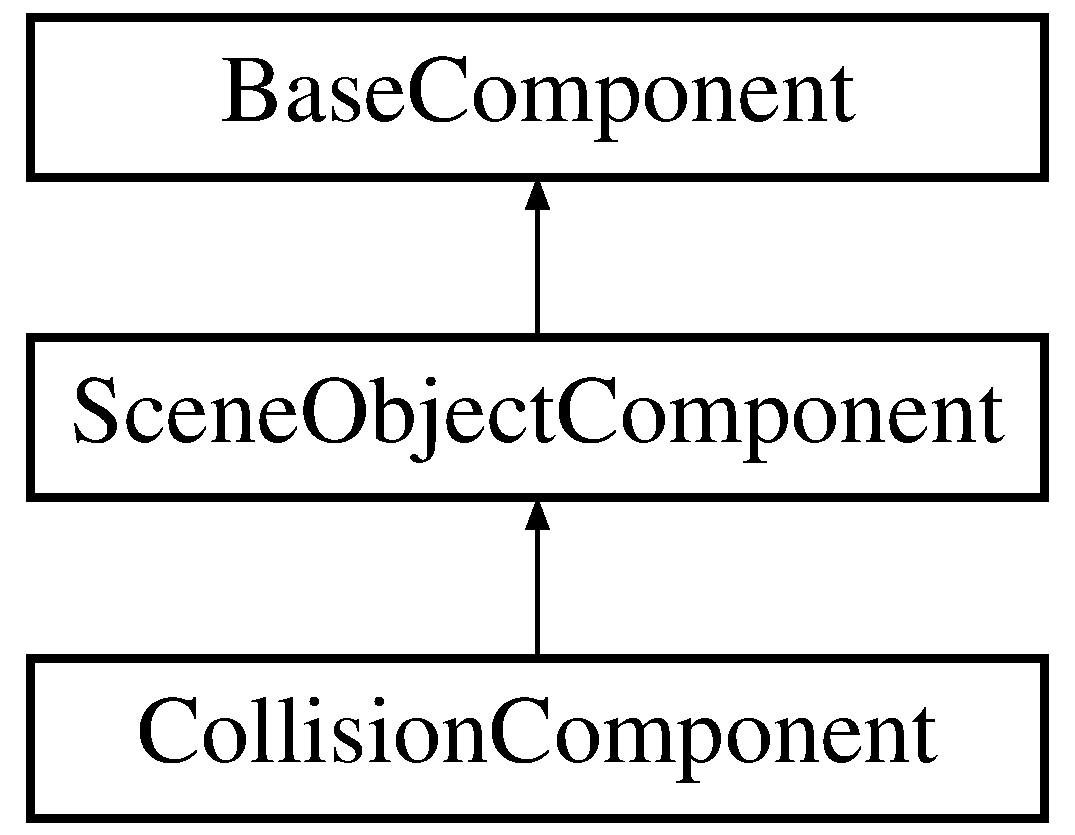
\includegraphics[height=3.000000cm]{class_collision_component}
\end{center}
\end{figure}
\subsection*{Public Member Functions}
\begin{DoxyCompactItemize}
\item 
\hyperlink{class_collision_component_a9fdf81792f07764fd9ee5d1c963aaff4}{Collision\+Component} (\hyperlink{class_scene_object}{Scene\+Object} $\ast$parent, std\+::weak\+\_\+ptr$<$ \hyperlink{class_meta_manager}{Meta\+Manager} $>$ managers, const glm\+::vec3 \&top\+Left\+Offset, const glm\+::vec3 \&bottom\+Right\+Offset)
\begin{DoxyCompactList}\small\item\em Default constructor. \end{DoxyCompactList}\item 
\hyperlink{class_collision_component_a8927f6bcecb9862b870426af970ab3b7}{$\sim$\+Collision\+Component} ()
\begin{DoxyCompactList}\small\item\em Default destructor. \end{DoxyCompactList}\item 
void \hyperlink{class_collision_component_aee9d681edd938781127af2249b750125}{step} (double dt) override
\begin{DoxyCompactList}\small\item\em Step the simulation state. \end{DoxyCompactList}\item 
void \hyperlink{class_collision_component_a322c2d4550aef70b8284465ae34278db}{predraw} (\hyperlink{class_context}{Context} $\ast$context) override
\begin{DoxyCompactList}\small\item\em Called before the renderer draws the scene This allows the scene objects to do updates that require a graphics context before the graphical state is drawn. \end{DoxyCompactList}\end{DoxyCompactItemize}
\subsection*{Additional Inherited Members}


\subsection{Detailed Description}
Component that describes collision information about the parent. 

This is currently setup to use Axis-\/\+Aligned Bounding Boxes, but the collision subsystem for it has been gutted. \begin{DoxyRefDesc}{Todo}
\item[\hyperlink{todo__todo000001}{Todo}]Setup collision geometry\end{DoxyRefDesc}


\begin{DoxyAuthor}{Author}
Hayley Hatton 
\end{DoxyAuthor}
\begin{DoxyDate}{Date}
06/03/2016 
\end{DoxyDate}
\begin{DoxySeeAlso}{See also}
\hyperlink{class_collision_manager}{Collision\+Manager} 
\end{DoxySeeAlso}


Definition at line 17 of file Collision\+Component.\+h.



\subsection{Constructor \& Destructor Documentation}
\index{Collision\+Component@{Collision\+Component}!Collision\+Component@{Collision\+Component}}
\index{Collision\+Component@{Collision\+Component}!Collision\+Component@{Collision\+Component}}
\subsubsection[{\texorpdfstring{Collision\+Component(\+Scene\+Object $\ast$parent, std\+::weak\+\_\+ptr$<$ Meta\+Manager $>$ managers, const glm\+::vec3 \&top\+Left\+Offset, const glm\+::vec3 \&bottom\+Right\+Offset)}{CollisionComponent(SceneObject *parent, std::weak_ptr< MetaManager > managers, const glm::vec3 &topLeftOffset, const glm::vec3 &bottomRightOffset)}}]{\setlength{\rightskip}{0pt plus 5cm}Collision\+Component\+::\+Collision\+Component (
\begin{DoxyParamCaption}
\item[{{\bf Scene\+Object} $\ast$}]{parent, }
\item[{std\+::weak\+\_\+ptr$<$ {\bf Meta\+Manager} $>$}]{managers, }
\item[{const glm\+::vec3 \&}]{top\+Left\+Offset, }
\item[{const glm\+::vec3 \&}]{bottom\+Right\+Offset}
\end{DoxyParamCaption}
)}\hypertarget{class_collision_component_a9fdf81792f07764fd9ee5d1c963aaff4}{}\label{class_collision_component_a9fdf81792f07764fd9ee5d1c963aaff4}


Default constructor. 


\begin{DoxyParams}{Parameters}
{\em parent} & Pointer to the scene object to attach component to \\
\hline
{\em managers} & Metamanager for accessing scene\textquotesingle{}s managers \\
\hline
\end{DoxyParams}


Definition at line 7 of file Collision\+Component.\+cpp.



References Message\+System\+::get\+Instance(), Scene\+Object\+Component\+::get\+Parent(), Collision\+Manager\+::register\+Collidable(), and Message\+System\+::subscribe().

\index{Collision\+Component@{Collision\+Component}!````~Collision\+Component@{$\sim$\+Collision\+Component}}
\index{````~Collision\+Component@{$\sim$\+Collision\+Component}!Collision\+Component@{Collision\+Component}}
\subsubsection[{\texorpdfstring{$\sim$\+Collision\+Component()}{~CollisionComponent()}}]{\setlength{\rightskip}{0pt plus 5cm}Collision\+Component\+::$\sim$\+Collision\+Component (
\begin{DoxyParamCaption}
{}
\end{DoxyParamCaption}
)}\hypertarget{class_collision_component_a8927f6bcecb9862b870426af970ab3b7}{}\label{class_collision_component_a8927f6bcecb9862b870426af970ab3b7}


Default destructor. 



Definition at line 25 of file Collision\+Component.\+cpp.



References Message\+System\+::get\+Instance(), Scene\+Object\+Component\+::get\+Parent(), Scene\+Object\+Component\+::m\+\_\+\+Managers, Collision\+Manager\+::unregister\+Collidable(), and Message\+System\+::unsubscribe().



\subsection{Member Function Documentation}
\index{Collision\+Component@{Collision\+Component}!predraw@{predraw}}
\index{predraw@{predraw}!Collision\+Component@{Collision\+Component}}
\subsubsection[{\texorpdfstring{predraw(\+Context $\ast$context) override}{predraw(Context *context) override}}]{\setlength{\rightskip}{0pt plus 5cm}void Collision\+Component\+::predraw (
\begin{DoxyParamCaption}
\item[{{\bf Context} $\ast$}]{context}
\end{DoxyParamCaption}
)\hspace{0.3cm}{\ttfamily [inline]}, {\ttfamily [override]}, {\ttfamily [virtual]}}\hypertarget{class_collision_component_a322c2d4550aef70b8284465ae34278db}{}\label{class_collision_component_a322c2d4550aef70b8284465ae34278db}


Called before the renderer draws the scene This allows the scene objects to do updates that require a graphics context before the graphical state is drawn. 


\begin{DoxyParams}{Parameters}
{\em context} & Graphics context \\
\hline
\end{DoxyParams}


Implements \hyperlink{class_scene_object_component_a7110e37ad23a708c2bf9828c7fd7df2f}{Scene\+Object\+Component}.



Definition at line 55 of file Collision\+Component.\+h.

\index{Collision\+Component@{Collision\+Component}!step@{step}}
\index{step@{step}!Collision\+Component@{Collision\+Component}}
\subsubsection[{\texorpdfstring{step(double dt) override}{step(double dt) override}}]{\setlength{\rightskip}{0pt plus 5cm}void Collision\+Component\+::step (
\begin{DoxyParamCaption}
\item[{double}]{dt}
\end{DoxyParamCaption}
)\hspace{0.3cm}{\ttfamily [inline]}, {\ttfamily [override]}, {\ttfamily [virtual]}}\hypertarget{class_collision_component_aee9d681edd938781127af2249b750125}{}\label{class_collision_component_aee9d681edd938781127af2249b750125}


Step the simulation state. 


\begin{DoxyParams}{Parameters}
{\em dt} & Delta-\/time since last step call in seconds \\
\hline
\end{DoxyParams}


Implements \hyperlink{class_scene_object_component_a99ebed011a6547be4d31a09927e3b810}{Scene\+Object\+Component}.



Definition at line 47 of file Collision\+Component.\+h.



The documentation for this class was generated from the following files\+:\begin{DoxyCompactItemize}
\item 
Lunar\+Drift/engine/components/\hyperlink{_collision_component_8h}{Collision\+Component.\+h}\item 
Lunar\+Drift/engine/components/\hyperlink{_collision_component_8cpp}{Collision\+Component.\+cpp}\end{DoxyCompactItemize}

\hypertarget{class_collision_manager}{}\section{Collision\+Manager Class Reference}
\label{class_collision_manager}\index{Collision\+Manager@{Collision\+Manager}}


A manager class for encapsulating collision detection processes.  




{\ttfamily \#include $<$Collision\+Manager.\+h$>$}

Inheritance diagram for Collision\+Manager\+:\begin{figure}[H]
\begin{center}
\leavevmode
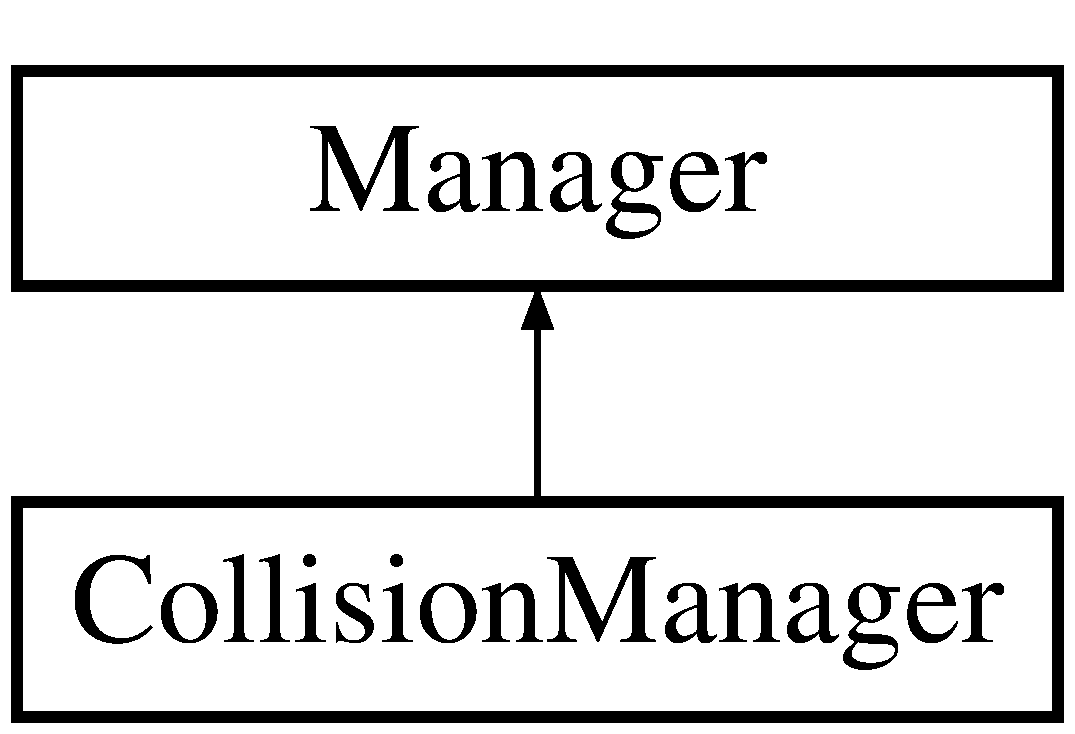
\includegraphics[height=2.000000cm]{class_collision_manager}
\end{center}
\end{figure}
\subsection*{Public Member Functions}
\begin{DoxyCompactItemize}
\item 
\hyperlink{class_collision_manager_a81f0b3f0cc0268c80f54714cd7ddb55f}{Collision\+Manager} ()
\begin{DoxyCompactList}\small\item\em Default constructor. \end{DoxyCompactList}\item 
\hyperlink{class_collision_manager_acdbb3c842f0ef1c7a028d3f080855766}{$\sim$\+Collision\+Manager} ()
\begin{DoxyCompactList}\small\item\em Default destructor. \end{DoxyCompactList}\item 
void \hyperlink{class_collision_manager_ac25d21cc6d3b44fc6b2fcc1dca9ca3f7}{register\+Collidable} (std\+::weak\+\_\+ptr$<$ \hyperlink{class_collision_component}{Collision\+Component} $>$ collidable)
\begin{DoxyCompactList}\small\item\em Set a collision component to be checked for collisions. \end{DoxyCompactList}\item 
void \hyperlink{class_collision_manager_ad54a09438c86f207fe69694fb49a15d4}{unregister\+Collidable} (std\+::weak\+\_\+ptr$<$ \hyperlink{class_collision_component}{Collision\+Component} $>$ collidable)
\begin{DoxyCompactList}\small\item\em Remove a collision component from being checked for collisions. \end{DoxyCompactList}\item 
void \hyperlink{class_collision_manager_ab10987e9a5f454973aa5eec45229d17a}{do\+Collisions} ()
\begin{DoxyCompactList}\small\item\em Check for collisions and dispatch appropriate messages. \end{DoxyCompactList}\end{DoxyCompactItemize}
\subsection*{Private Attributes}
\begin{DoxyCompactItemize}
\item 
std\+::list$<$ std\+::weak\+\_\+ptr$<$ \hyperlink{class_collision_component}{Collision\+Component} $>$ $>$ \hyperlink{class_collision_manager_a1e8ca739d58f92f5bae1d4dea802adcc}{m\+\_\+\+Collidables}
\end{DoxyCompactItemize}


\subsection{Detailed Description}
A manager class for encapsulating collision detection processes. 

\begin{DoxyAuthor}{Author}
Hayley Hatton 
\end{DoxyAuthor}
\begin{DoxyDate}{Date}
13/03/2016 
\end{DoxyDate}
\begin{DoxySeeAlso}{See also}
\hyperlink{class_scene}{Scene} 
\end{DoxySeeAlso}


Definition at line 14 of file Collision\+Manager.\+h.



\subsection{Constructor \& Destructor Documentation}
\index{Collision\+Manager@{Collision\+Manager}!Collision\+Manager@{Collision\+Manager}}
\index{Collision\+Manager@{Collision\+Manager}!Collision\+Manager@{Collision\+Manager}}
\subsubsection[{\texorpdfstring{Collision\+Manager()}{CollisionManager()}}]{\setlength{\rightskip}{0pt plus 5cm}Collision\+Manager\+::\+Collision\+Manager (
\begin{DoxyParamCaption}
{}
\end{DoxyParamCaption}
)}\hypertarget{class_collision_manager_a81f0b3f0cc0268c80f54714cd7ddb55f}{}\label{class_collision_manager_a81f0b3f0cc0268c80f54714cd7ddb55f}


Default constructor. 



Definition at line 6 of file Collision\+Manager.\+cpp.

\index{Collision\+Manager@{Collision\+Manager}!````~Collision\+Manager@{$\sim$\+Collision\+Manager}}
\index{````~Collision\+Manager@{$\sim$\+Collision\+Manager}!Collision\+Manager@{Collision\+Manager}}
\subsubsection[{\texorpdfstring{$\sim$\+Collision\+Manager()}{~CollisionManager()}}]{\setlength{\rightskip}{0pt plus 5cm}Collision\+Manager\+::$\sim$\+Collision\+Manager (
\begin{DoxyParamCaption}
{}
\end{DoxyParamCaption}
)}\hypertarget{class_collision_manager_acdbb3c842f0ef1c7a028d3f080855766}{}\label{class_collision_manager_acdbb3c842f0ef1c7a028d3f080855766}


Default destructor. 



Definition at line 10 of file Collision\+Manager.\+cpp.



\subsection{Member Function Documentation}
\index{Collision\+Manager@{Collision\+Manager}!do\+Collisions@{do\+Collisions}}
\index{do\+Collisions@{do\+Collisions}!Collision\+Manager@{Collision\+Manager}}
\subsubsection[{\texorpdfstring{do\+Collisions()}{doCollisions()}}]{\setlength{\rightskip}{0pt plus 5cm}void Collision\+Manager\+::do\+Collisions (
\begin{DoxyParamCaption}
{}
\end{DoxyParamCaption}
)}\hypertarget{class_collision_manager_ab10987e9a5f454973aa5eec45229d17a}{}\label{class_collision_manager_ab10987e9a5f454973aa5eec45229d17a}


Check for collisions and dispatch appropriate messages. 



Definition at line 38 of file Collision\+Manager.\+cpp.



References m\+\_\+\+Collidables.



Referenced by Scene\+::step().

\index{Collision\+Manager@{Collision\+Manager}!register\+Collidable@{register\+Collidable}}
\index{register\+Collidable@{register\+Collidable}!Collision\+Manager@{Collision\+Manager}}
\subsubsection[{\texorpdfstring{register\+Collidable(std\+::weak\+\_\+ptr$<$ Collision\+Component $>$ collidable)}{registerCollidable(std::weak_ptr< CollisionComponent > collidable)}}]{\setlength{\rightskip}{0pt plus 5cm}void Collision\+Manager\+::register\+Collidable (
\begin{DoxyParamCaption}
\item[{std\+::weak\+\_\+ptr$<$ {\bf Collision\+Component} $>$}]{collidable}
\end{DoxyParamCaption}
)}\hypertarget{class_collision_manager_ac25d21cc6d3b44fc6b2fcc1dca9ca3f7}{}\label{class_collision_manager_ac25d21cc6d3b44fc6b2fcc1dca9ca3f7}


Set a collision component to be checked for collisions. 


\begin{DoxyParams}{Parameters}
{\em collidable} & Reference to a component for describing collisions \\
\hline
\end{DoxyParams}


Definition at line 15 of file Collision\+Manager.\+cpp.



References m\+\_\+\+Collidables.



Referenced by Collision\+Component\+::\+Collision\+Component().

\index{Collision\+Manager@{Collision\+Manager}!unregister\+Collidable@{unregister\+Collidable}}
\index{unregister\+Collidable@{unregister\+Collidable}!Collision\+Manager@{Collision\+Manager}}
\subsubsection[{\texorpdfstring{unregister\+Collidable(std\+::weak\+\_\+ptr$<$ Collision\+Component $>$ collidable)}{unregisterCollidable(std::weak_ptr< CollisionComponent > collidable)}}]{\setlength{\rightskip}{0pt plus 5cm}void Collision\+Manager\+::unregister\+Collidable (
\begin{DoxyParamCaption}
\item[{std\+::weak\+\_\+ptr$<$ {\bf Collision\+Component} $>$}]{collidable}
\end{DoxyParamCaption}
)}\hypertarget{class_collision_manager_ad54a09438c86f207fe69694fb49a15d4}{}\label{class_collision_manager_ad54a09438c86f207fe69694fb49a15d4}


Remove a collision component from being checked for collisions. 


\begin{DoxyParams}{Parameters}
{\em collidable} & Reference to a component for describing collisions \\
\hline
\end{DoxyParams}


Definition at line 21 of file Collision\+Manager.\+cpp.



References c, and m\+\_\+\+Collidables.



Referenced by Collision\+Component\+::$\sim$\+Collision\+Component().



\subsection{Member Data Documentation}
\index{Collision\+Manager@{Collision\+Manager}!m\+\_\+\+Collidables@{m\+\_\+\+Collidables}}
\index{m\+\_\+\+Collidables@{m\+\_\+\+Collidables}!Collision\+Manager@{Collision\+Manager}}
\subsubsection[{\texorpdfstring{m\+\_\+\+Collidables}{m_Collidables}}]{\setlength{\rightskip}{0pt plus 5cm}std\+::list$<$std\+::weak\+\_\+ptr$<${\bf Collision\+Component}$>$ $>$ Collision\+Manager\+::m\+\_\+\+Collidables\hspace{0.3cm}{\ttfamily [private]}}\hypertarget{class_collision_manager_a1e8ca739d58f92f5bae1d4dea802adcc}{}\label{class_collision_manager_a1e8ca739d58f92f5bae1d4dea802adcc}


Definition at line 45 of file Collision\+Manager.\+h.



Referenced by do\+Collisions(), register\+Collidable(), and unregister\+Collidable().



The documentation for this class was generated from the following files\+:\begin{DoxyCompactItemize}
\item 
Lunar\+Drift/engine/managers/\hyperlink{_collision_manager_8h}{Collision\+Manager.\+h}\item 
Lunar\+Drift/engine/managers/\hyperlink{_collision_manager_8cpp}{Collision\+Manager.\+cpp}\end{DoxyCompactItemize}

\hypertarget{class_collision_message}{}\section{Collision\+Message Class Reference}
\label{class_collision_message}\index{Collision\+Message@{Collision\+Message}}


{\ttfamily \#include $<$Collision\+Message.\+h$>$}

Inheritance diagram for Collision\+Message\+:\begin{figure}[H]
\begin{center}
\leavevmode
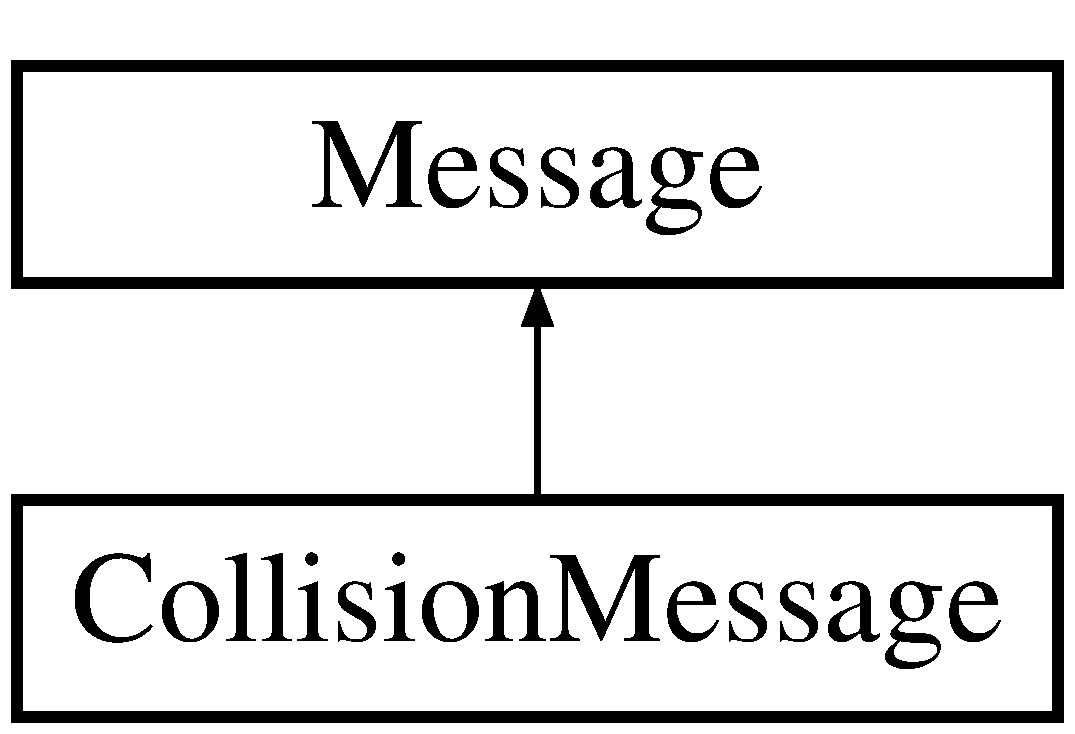
\includegraphics[height=2.000000cm]{class_collision_message}
\end{center}
\end{figure}
\subsection*{Public Member Functions}
\begin{DoxyCompactItemize}
\item 
\hyperlink{class_collision_message_a36f3e8a87d92faa7f3e57a3c596540b1}{Collision\+Message} (\hyperlink{class_scene_object}{Scene\+Object} $\ast$partner)
\item 
virtual \hyperlink{class_collision_message_a2aa8a6168bfb639726cad05c46f1c987}{$\sim$\+Collision\+Message} ()
\item 
\hyperlink{class_scene_object}{Scene\+Object} $\ast$ \hyperlink{class_collision_message_ad760873a6bff76eebab3e21238a35424}{get\+Partner} ()
\end{DoxyCompactItemize}
\subsection*{Private Attributes}
\begin{DoxyCompactItemize}
\item 
\hyperlink{class_scene_object}{Scene\+Object} $\ast$ \hyperlink{class_collision_message_af8a6bd9fda3bf5a09b7132d13f548073}{m\+\_\+\+Partner}
\end{DoxyCompactItemize}


\subsection{Detailed Description}


Definition at line 6 of file Collision\+Message.\+h.



\subsection{Constructor \& Destructor Documentation}
\index{Collision\+Message@{Collision\+Message}!Collision\+Message@{Collision\+Message}}
\index{Collision\+Message@{Collision\+Message}!Collision\+Message@{Collision\+Message}}
\subsubsection[{\texorpdfstring{Collision\+Message(\+Scene\+Object $\ast$partner)}{CollisionMessage(SceneObject *partner)}}]{\setlength{\rightskip}{0pt plus 5cm}Collision\+Message\+::\+Collision\+Message (
\begin{DoxyParamCaption}
\item[{{\bf Scene\+Object} $\ast$}]{partner}
\end{DoxyParamCaption}
)}\hypertarget{class_collision_message_a36f3e8a87d92faa7f3e57a3c596540b1}{}\label{class_collision_message_a36f3e8a87d92faa7f3e57a3c596540b1}


Definition at line 4 of file Collision\+Message.\+cpp.

\index{Collision\+Message@{Collision\+Message}!````~Collision\+Message@{$\sim$\+Collision\+Message}}
\index{````~Collision\+Message@{$\sim$\+Collision\+Message}!Collision\+Message@{Collision\+Message}}
\subsubsection[{\texorpdfstring{$\sim$\+Collision\+Message()}{~CollisionMessage()}}]{\setlength{\rightskip}{0pt plus 5cm}Collision\+Message\+::$\sim$\+Collision\+Message (
\begin{DoxyParamCaption}
{}
\end{DoxyParamCaption}
)\hspace{0.3cm}{\ttfamily [virtual]}}\hypertarget{class_collision_message_a2aa8a6168bfb639726cad05c46f1c987}{}\label{class_collision_message_a2aa8a6168bfb639726cad05c46f1c987}


Definition at line 10 of file Collision\+Message.\+cpp.



\subsection{Member Function Documentation}
\index{Collision\+Message@{Collision\+Message}!get\+Partner@{get\+Partner}}
\index{get\+Partner@{get\+Partner}!Collision\+Message@{Collision\+Message}}
\subsubsection[{\texorpdfstring{get\+Partner()}{getPartner()}}]{\setlength{\rightskip}{0pt plus 5cm}{\bf Scene\+Object}$\ast$ Collision\+Message\+::get\+Partner (
\begin{DoxyParamCaption}
{}
\end{DoxyParamCaption}
)\hspace{0.3cm}{\ttfamily [inline]}}\hypertarget{class_collision_message_ad760873a6bff76eebab3e21238a35424}{}\label{class_collision_message_ad760873a6bff76eebab3e21238a35424}


Definition at line 14 of file Collision\+Message.\+h.



References m\+\_\+\+Partner.



\subsection{Member Data Documentation}
\index{Collision\+Message@{Collision\+Message}!m\+\_\+\+Partner@{m\+\_\+\+Partner}}
\index{m\+\_\+\+Partner@{m\+\_\+\+Partner}!Collision\+Message@{Collision\+Message}}
\subsubsection[{\texorpdfstring{m\+\_\+\+Partner}{m_Partner}}]{\setlength{\rightskip}{0pt plus 5cm}{\bf Scene\+Object}$\ast$ Collision\+Message\+::m\+\_\+\+Partner\hspace{0.3cm}{\ttfamily [private]}}\hypertarget{class_collision_message_af8a6bd9fda3bf5a09b7132d13f548073}{}\label{class_collision_message_af8a6bd9fda3bf5a09b7132d13f548073}


Definition at line 17 of file Collision\+Message.\+h.



Referenced by get\+Partner().



The documentation for this class was generated from the following files\+:\begin{DoxyCompactItemize}
\item 
Lunar\+Drift/engine/comms/predefined/\hyperlink{_collision_message_8h}{Collision\+Message.\+h}\item 
Lunar\+Drift/engine/comms/predefined/\hyperlink{_collision_message_8cpp}{Collision\+Message.\+cpp}\end{DoxyCompactItemize}

\hypertarget{class_config}{}\section{Config Class Reference}
\label{class_config}\index{Config@{Config}}


A singleton that aggregates and encaspsulates access to config files.  




{\ttfamily \#include $<$Config.\+h$>$}

\subsection*{Public Member Functions}
\begin{DoxyCompactItemize}
\item 
void \hyperlink{class_config_a8198223ee3542b0754720c28f1ca8e42}{load} (const std\+::string \&file)
\begin{DoxyCompactList}\small\item\em Load an I\+NI file into the configuration settings database. \end{DoxyCompactList}\item 
void \hyperlink{class_config_a095b729166d151267aea1e969e02a5e0}{save} (const std\+::string \&file)
\begin{DoxyCompactList}\small\item\em Save to an I\+NI file from the configuration settings database. \end{DoxyCompactList}\item 
void \hyperlink{class_config_a8159645eaab244229fb539bd7f23d365}{save\+All} ()
\begin{DoxyCompactList}\small\item\em Save all loaded configuration files with current settings. \end{DoxyCompactList}\item 
const std\+::string \& \hyperlink{class_config_a14108dcb3ce428431483cd4107fb6074}{get} (const std\+::string \&file, const std\+::string \&name) const 
\begin{DoxyCompactList}\small\item\em Access a setting from a loaded configuration file. \end{DoxyCompactList}\item 
int \hyperlink{class_config_a385fbc7610cfa7fa4fb11b11d6fad26a}{get\+Int} (const std\+::string \&file, const std\+::string \&name) const 
\begin{DoxyCompactList}\small\item\em Access a setting from a loaded configuration file. \end{DoxyCompactList}\item 
bool \hyperlink{class_config_a28fdb5bcf67d57b5df952e9f667f313f}{get\+Bool} (const std\+::string \&file, const std\+::string \&name, bool unknown\+Is\+False=true) const 
\begin{DoxyCompactList}\small\item\em Access a setting from a loaded configuration file. \end{DoxyCompactList}\item 
double \hyperlink{class_config_aaa35e0251f6920bf5cb42c8c1edad6f7}{get\+Double} (const std\+::string \&file, const std\+::string \&name) const 
\begin{DoxyCompactList}\small\item\em Access a setting from a loaded configuration file. \end{DoxyCompactList}\item 
float \hyperlink{class_config_acd8be5c460303ba4a5df8036f99e5935}{get\+Float} (const std\+::string \&file, const std\+::string \&name) const 
\begin{DoxyCompactList}\small\item\em Access a setting from a loaded configuration file. \end{DoxyCompactList}\item 
void \hyperlink{class_config_a95d6afbbffc9cfa02a9d1171d48c9e8b}{set} (const std\+::string \&file, const std\+::string \&name, const std\+::string value)
\begin{DoxyCompactList}\small\item\em Set a setting in the configuration database. \end{DoxyCompactList}\item 
void \hyperlink{class_config_a3cd33d32e89a8831a7047653c217d760}{set} (const std\+::string \&file, const std\+::string \&name, int value)
\begin{DoxyCompactList}\small\item\em Set a setting in the configuration database. \end{DoxyCompactList}\item 
void \hyperlink{class_config_ac2b0c38ab146ff4e2de8dbe10fc08b36}{set} (const std\+::string \&file, const std\+::string \&name, bool value)
\begin{DoxyCompactList}\small\item\em Set a setting in the configuration database. \end{DoxyCompactList}\item 
void \hyperlink{class_config_adc58efca4fe18f3338b82b3cbe7d6f94}{set} (const std\+::string \&file, const std\+::string \&name, double value)
\begin{DoxyCompactList}\small\item\em Set a setting in the configuration database. \end{DoxyCompactList}\end{DoxyCompactItemize}
\subsection*{Static Public Member Functions}
\begin{DoxyCompactItemize}
\item 
static \hyperlink{class_config}{Config} \& \hyperlink{class_config_a5154d96acc76c1fae8c564f3705fe197}{get} ()
\begin{DoxyCompactList}\small\item\em Access the singleton instance. \end{DoxyCompactList}\end{DoxyCompactItemize}
\subsection*{Private Member Functions}
\begin{DoxyCompactItemize}
\item 
\hyperlink{class_config_abd0c571c116924871e30444b192b792a}{Config} ()
\item 
\hyperlink{class_config_a43fa97921860bb03437dde7461310459}{Config} (\hyperlink{class_config}{Config} const \&)
\item 
void \hyperlink{class_config_a9b6a7f8721a8789102928869dc1e186c}{operator=} (\hyperlink{class_config}{Config} const \&)
\end{DoxyCompactItemize}
\subsection*{Private Attributes}
\begin{DoxyCompactItemize}
\item 
std\+::map$<$ std\+::string, std\+::map$<$ std\+::string, std\+::string $>$ $>$ \hyperlink{class_config_a5c864239797e10af1a62b292d7ededad}{m\+\_\+\+File\+Data}
\begin{DoxyCompactList}\small\item\em Settings database. \end{DoxyCompactList}\end{DoxyCompactItemize}


\subsection{Detailed Description}
A singleton that aggregates and encaspsulates access to config files. 

Most projects utilize .I\+NI files to configure the program. They provide convenient storage places for configuration variables, and are both easily readable and modifiable by users from outside of the program. This singleton class allows these I\+NI files to be conveniently handled and interfaced for easier use by programmers.

\begin{DoxyNote}{Note}
\char`\"{}\+\_\+engine\char`\"{} file is a virtual file for representing internal engine configuration states
\end{DoxyNote}
\begin{DoxyAuthor}{Author}
Hayley Hatton 
\end{DoxyAuthor}
\begin{DoxyDate}{Date}
20/02/2016 
\end{DoxyDate}
\begin{DoxyRefDesc}{Todo}
\item[\hyperlink{todo__todo000004}{Todo}](Hayley\#3\#20/02/16)\+: Directory control. 

(Hayley\#2\#20/02/16)\+: Access via \mbox{[}\mbox{]} operators? \end{DoxyRefDesc}


Definition at line 22 of file Config.\+h.



\subsection{Constructor \& Destructor Documentation}
\index{Config@{Config}!Config@{Config}}
\index{Config@{Config}!Config@{Config}}
\subsubsection[{\texorpdfstring{Config()}{Config()}}]{\setlength{\rightskip}{0pt plus 5cm}Config\+::\+Config (
\begin{DoxyParamCaption}
{}
\end{DoxyParamCaption}
)\hspace{0.3cm}{\ttfamily [inline]}, {\ttfamily [private]}}\hypertarget{class_config_abd0c571c116924871e30444b192b792a}{}\label{class_config_abd0c571c116924871e30444b192b792a}


Definition at line 160 of file Config.\+h.



References operator=().

\index{Config@{Config}!Config@{Config}}
\index{Config@{Config}!Config@{Config}}
\subsubsection[{\texorpdfstring{Config(\+Config const \&)}{Config(Config const &)}}]{\setlength{\rightskip}{0pt plus 5cm}Config\+::\+Config (
\begin{DoxyParamCaption}
\item[{{\bf Config} const \&}]{}
\end{DoxyParamCaption}
)\hspace{0.3cm}{\ttfamily [private]}}\hypertarget{class_config_a43fa97921860bb03437dde7461310459}{}\label{class_config_a43fa97921860bb03437dde7461310459}


\subsection{Member Function Documentation}
\index{Config@{Config}!get@{get}}
\index{get@{get}!Config@{Config}}
\subsubsection[{\texorpdfstring{get()}{get()}}]{\setlength{\rightskip}{0pt plus 5cm}static {\bf Config}\& Config\+::get (
\begin{DoxyParamCaption}
{}
\end{DoxyParamCaption}
)\hspace{0.3cm}{\ttfamily [inline]}, {\ttfamily [static]}}\hypertarget{class_config_a5154d96acc76c1fae8c564f3705fe197}{}\label{class_config_a5154d96acc76c1fae8c564f3705fe197}


Access the singleton instance. 

\begin{DoxyReturn}{Returns}
The actual \hyperlink{class_config}{Config} instance. 
\end{DoxyReturn}


Definition at line 29 of file Config.\+h.



References get\+Bool(), get\+Double(), get\+Float(), get\+Int(), load(), save(), and save\+All().



Referenced by Lunar\+Drift\+Program\+::\+Lunar\+Drift\+Program(), Shader\+Program\+::read\+Shader\+File(), Test\+Scene3\+D\+::set\+Size(), and Test\+Scene3\+D\+::\+Test\+Scene3\+D().

\index{Config@{Config}!get@{get}}
\index{get@{get}!Config@{Config}}
\subsubsection[{\texorpdfstring{get(const std\+::string \&file, const std\+::string \&name) const }{get(const std::string &file, const std::string &name) const }}]{\setlength{\rightskip}{0pt plus 5cm}const std\+::string \& Config\+::get (
\begin{DoxyParamCaption}
\item[{const std\+::string \&}]{file, }
\item[{const std\+::string \&}]{name}
\end{DoxyParamCaption}
) const}\hypertarget{class_config_a14108dcb3ce428431483cd4107fb6074}{}\label{class_config_a14108dcb3ce428431483cd4107fb6074}


Access a setting from a loaded configuration file. 


\begin{DoxyParams}{Parameters}
{\em file} & Name of the I\+NI file, without the .ini extension. \\
\hline
{\em name} & Configuration setting to query. \\
\hline
\end{DoxyParams}
\begin{DoxyReturn}{Returns}
String value associated with the queried setting. 
\end{DoxyReturn}

\begin{DoxyExceptions}{Exceptions}
{\em \hyperlink{class_configuration_exception}{Configuration\+Exception}} & \\
\hline
\end{DoxyExceptions}


Definition at line 124 of file Config.\+cpp.



References m\+\_\+\+File\+Data.

\index{Config@{Config}!get\+Bool@{get\+Bool}}
\index{get\+Bool@{get\+Bool}!Config@{Config}}
\subsubsection[{\texorpdfstring{get\+Bool(const std\+::string \&file, const std\+::string \&name, bool unknown\+Is\+False=true) const }{getBool(const std::string &file, const std::string &name, bool unknownIsFalse=true) const }}]{\setlength{\rightskip}{0pt plus 5cm}bool Config\+::get\+Bool (
\begin{DoxyParamCaption}
\item[{const std\+::string \&}]{file, }
\item[{const std\+::string \&}]{name, }
\item[{bool}]{unknown\+Is\+False = {\ttfamily true}}
\end{DoxyParamCaption}
) const}\hypertarget{class_config_a28fdb5bcf67d57b5df952e9f667f313f}{}\label{class_config_a28fdb5bcf67d57b5df952e9f667f313f}


Access a setting from a loaded configuration file. 


\begin{DoxyParams}{Parameters}
{\em file} & Name of the I\+NI file, without the .ini extension. \\
\hline
{\em name} & Configuration setting to query. \\
\hline
\end{DoxyParams}
\begin{DoxyReturn}{Returns}
True/false value associated with the queried setting. 
\end{DoxyReturn}

\begin{DoxyExceptions}{Exceptions}
{\em \hyperlink{class_configuration_exception}{Configuration\+Exception}} & \\
\hline
\end{DoxyExceptions}


Definition at line 163 of file Config.\+cpp.



Referenced by get().

\index{Config@{Config}!get\+Double@{get\+Double}}
\index{get\+Double@{get\+Double}!Config@{Config}}
\subsubsection[{\texorpdfstring{get\+Double(const std\+::string \&file, const std\+::string \&name) const }{getDouble(const std::string &file, const std::string &name) const }}]{\setlength{\rightskip}{0pt plus 5cm}double Config\+::get\+Double (
\begin{DoxyParamCaption}
\item[{const std\+::string \&}]{file, }
\item[{const std\+::string \&}]{name}
\end{DoxyParamCaption}
) const}\hypertarget{class_config_aaa35e0251f6920bf5cb42c8c1edad6f7}{}\label{class_config_aaa35e0251f6920bf5cb42c8c1edad6f7}


Access a setting from a loaded configuration file. 


\begin{DoxyParams}{Parameters}
{\em file} & Name of the I\+NI file, without the .ini extension. \\
\hline
{\em name} & Configuration setting to query. \\
\hline
\end{DoxyParams}
\begin{DoxyReturn}{Returns}
Double-\/precision decimal associated with the queried setting. 
\end{DoxyReturn}

\begin{DoxyExceptions}{Exceptions}
{\em \hyperlink{class_configuration_exception}{Configuration\+Exception}} & \\
\hline
\end{DoxyExceptions}


Definition at line 194 of file Config.\+cpp.



Referenced by get().

\index{Config@{Config}!get\+Float@{get\+Float}}
\index{get\+Float@{get\+Float}!Config@{Config}}
\subsubsection[{\texorpdfstring{get\+Float(const std\+::string \&file, const std\+::string \&name) const }{getFloat(const std::string &file, const std::string &name) const }}]{\setlength{\rightskip}{0pt plus 5cm}float Config\+::get\+Float (
\begin{DoxyParamCaption}
\item[{const std\+::string \&}]{file, }
\item[{const std\+::string \&}]{name}
\end{DoxyParamCaption}
) const}\hypertarget{class_config_acd8be5c460303ba4a5df8036f99e5935}{}\label{class_config_acd8be5c460303ba4a5df8036f99e5935}


Access a setting from a loaded configuration file. 


\begin{DoxyParams}{Parameters}
{\em file} & Name of the I\+NI file, without the .ini extension. \\
\hline
{\em name} & Configuration setting to query. \\
\hline
\end{DoxyParams}
\begin{DoxyReturn}{Returns}
Floating-\/point decimal associated with the queried setting. 
\end{DoxyReturn}

\begin{DoxyExceptions}{Exceptions}
{\em \hyperlink{class_configuration_exception}{Configuration\+Exception}} & \\
\hline
\end{DoxyExceptions}


Definition at line 211 of file Config.\+cpp.



Referenced by get(), Test\+Scene3\+D\+::set\+Size(), and Test\+Scene3\+D\+::\+Test\+Scene3\+D().

\index{Config@{Config}!get\+Int@{get\+Int}}
\index{get\+Int@{get\+Int}!Config@{Config}}
\subsubsection[{\texorpdfstring{get\+Int(const std\+::string \&file, const std\+::string \&name) const }{getInt(const std::string &file, const std::string &name) const }}]{\setlength{\rightskip}{0pt plus 5cm}int Config\+::get\+Int (
\begin{DoxyParamCaption}
\item[{const std\+::string \&}]{file, }
\item[{const std\+::string \&}]{name}
\end{DoxyParamCaption}
) const}\hypertarget{class_config_a385fbc7610cfa7fa4fb11b11d6fad26a}{}\label{class_config_a385fbc7610cfa7fa4fb11b11d6fad26a}


Access a setting from a loaded configuration file. 


\begin{DoxyParams}{Parameters}
{\em file} & Name of the I\+NI file, without the .ini extension. \\
\hline
{\em name} & Configuration setting to query. \\
\hline
\end{DoxyParams}
\begin{DoxyReturn}{Returns}
Signed integer associated with the queried setting. 
\end{DoxyReturn}

\begin{DoxyExceptions}{Exceptions}
{\em \hyperlink{class_configuration_exception}{Configuration\+Exception}} & \\
\hline
\end{DoxyExceptions}


Definition at line 146 of file Config.\+cpp.



Referenced by get().

\index{Config@{Config}!load@{load}}
\index{load@{load}!Config@{Config}}
\subsubsection[{\texorpdfstring{load(const std\+::string \&file)}{load(const std::string &file)}}]{\setlength{\rightskip}{0pt plus 5cm}void Config\+::load (
\begin{DoxyParamCaption}
\item[{const std\+::string \&}]{file}
\end{DoxyParamCaption}
)}\hypertarget{class_config_a8198223ee3542b0754720c28f1ca8e42}{}\label{class_config_a8198223ee3542b0754720c28f1ca8e42}


Load an I\+NI file into the configuration settings database. 


\begin{DoxyParams}{Parameters}
{\em file} & Name of the I\+NI file, without the .ini extension. \\
\hline
\end{DoxyParams}

\begin{DoxyExceptions}{Exceptions}
{\em \hyperlink{class_file_i_o_exception}{File\+I\+O\+Exception}} & \\
\hline
\end{DoxyExceptions}


Definition at line 27 of file Config.\+cpp.



References m\+\_\+\+File\+Data, and trim().



Referenced by get(), and Lunar\+Drift\+Program\+::\+Lunar\+Drift\+Program().

\index{Config@{Config}!operator=@{operator=}}
\index{operator=@{operator=}!Config@{Config}}
\subsubsection[{\texorpdfstring{operator=(\+Config const \&)}{operator=(Config const &)}}]{\setlength{\rightskip}{0pt plus 5cm}void Config\+::operator= (
\begin{DoxyParamCaption}
\item[{{\bf Config} const \&}]{}
\end{DoxyParamCaption}
)\hspace{0.3cm}{\ttfamily [private]}}\hypertarget{class_config_a9b6a7f8721a8789102928869dc1e186c}{}\label{class_config_a9b6a7f8721a8789102928869dc1e186c}


Referenced by Config().

\index{Config@{Config}!save@{save}}
\index{save@{save}!Config@{Config}}
\subsubsection[{\texorpdfstring{save(const std\+::string \&file)}{save(const std::string &file)}}]{\setlength{\rightskip}{0pt plus 5cm}void Config\+::save (
\begin{DoxyParamCaption}
\item[{const std\+::string \&}]{file}
\end{DoxyParamCaption}
)}\hypertarget{class_config_a095b729166d151267aea1e969e02a5e0}{}\label{class_config_a095b729166d151267aea1e969e02a5e0}


Save to an I\+NI file from the configuration settings database. 


\begin{DoxyParams}{Parameters}
{\em file} & Name of the I\+NI file, without the .ini extension. \\
\hline
\end{DoxyParams}

\begin{DoxyExceptions}{Exceptions}
{\em \hyperlink{class_file_i_o_exception}{File\+I\+O\+Exception}} & \\
\hline
\end{DoxyExceptions}
\begin{DoxyRefDesc}{Todo}
\item[\hyperlink{todo__todo000003}{Todo}](Hayley\#2\#09/24/15)\+: Put I\+NI sections together to obey the standards better \end{DoxyRefDesc}


Definition at line 78 of file Config.\+cpp.



References m\+\_\+\+File\+Data.



Referenced by get(), and save\+All().

\index{Config@{Config}!save\+All@{save\+All}}
\index{save\+All@{save\+All}!Config@{Config}}
\subsubsection[{\texorpdfstring{save\+All()}{saveAll()}}]{\setlength{\rightskip}{0pt plus 5cm}void Config\+::save\+All (
\begin{DoxyParamCaption}
{}
\end{DoxyParamCaption}
)}\hypertarget{class_config_a8159645eaab244229fb539bd7f23d365}{}\label{class_config_a8159645eaab244229fb539bd7f23d365}


Save all loaded configuration files with current settings. 



Definition at line 118 of file Config.\+cpp.



References m\+\_\+\+File\+Data, and save().



Referenced by get().

\index{Config@{Config}!set@{set}}
\index{set@{set}!Config@{Config}}
\subsubsection[{\texorpdfstring{set(const std\+::string \&file, const std\+::string \&name, const std\+::string value)}{set(const std::string &file, const std::string &name, const std::string value)}}]{\setlength{\rightskip}{0pt plus 5cm}void Config\+::set (
\begin{DoxyParamCaption}
\item[{const std\+::string \&}]{file, }
\item[{const std\+::string \&}]{name, }
\item[{const std\+::string}]{value}
\end{DoxyParamCaption}
)}\hypertarget{class_config_a95d6afbbffc9cfa02a9d1171d48c9e8b}{}\label{class_config_a95d6afbbffc9cfa02a9d1171d48c9e8b}


Set a setting in the configuration database. 


\begin{DoxyParams}{Parameters}
{\em file} & Name of the I\+NI file, without the .ini extension. \\
\hline
{\em name} & Configuration setting to set value of. \\
\hline
{\em value} & String to set the setting to. \\
\hline
\end{DoxyParams}


Definition at line 228 of file Config.\+cpp.



References m\+\_\+\+File\+Data.



Referenced by Lunar\+Drift\+Program\+::\+Lunar\+Drift\+Program().

\index{Config@{Config}!set@{set}}
\index{set@{set}!Config@{Config}}
\subsubsection[{\texorpdfstring{set(const std\+::string \&file, const std\+::string \&name, int value)}{set(const std::string &file, const std::string &name, int value)}}]{\setlength{\rightskip}{0pt plus 5cm}void Config\+::set (
\begin{DoxyParamCaption}
\item[{const std\+::string \&}]{file, }
\item[{const std\+::string \&}]{name, }
\item[{int}]{value}
\end{DoxyParamCaption}
)}\hypertarget{class_config_a3cd33d32e89a8831a7047653c217d760}{}\label{class_config_a3cd33d32e89a8831a7047653c217d760}


Set a setting in the configuration database. 


\begin{DoxyParams}{Parameters}
{\em file} & Name of the I\+NI file, without the .ini extension. \\
\hline
{\em name} & Configuration setting to set value of. \\
\hline
{\em value} & Signed integer to set the setting to. \\
\hline
\end{DoxyParams}


Definition at line 239 of file Config.\+cpp.



References to\+\_\+wstring().

\index{Config@{Config}!set@{set}}
\index{set@{set}!Config@{Config}}
\subsubsection[{\texorpdfstring{set(const std\+::string \&file, const std\+::string \&name, bool value)}{set(const std::string &file, const std::string &name, bool value)}}]{\setlength{\rightskip}{0pt plus 5cm}void Config\+::set (
\begin{DoxyParamCaption}
\item[{const std\+::string \&}]{file, }
\item[{const std\+::string \&}]{name, }
\item[{bool}]{value}
\end{DoxyParamCaption}
)}\hypertarget{class_config_ac2b0c38ab146ff4e2de8dbe10fc08b36}{}\label{class_config_ac2b0c38ab146ff4e2de8dbe10fc08b36}


Set a setting in the configuration database. 


\begin{DoxyParams}{Parameters}
{\em file} & Name of the I\+NI file, without the .ini extension. \\
\hline
{\em name} & Configuration setting to set value of. \\
\hline
{\em value} & True/false value to set the setting to. \\
\hline
\end{DoxyParams}


Definition at line 250 of file Config.\+cpp.

\index{Config@{Config}!set@{set}}
\index{set@{set}!Config@{Config}}
\subsubsection[{\texorpdfstring{set(const std\+::string \&file, const std\+::string \&name, double value)}{set(const std::string &file, const std::string &name, double value)}}]{\setlength{\rightskip}{0pt plus 5cm}void Config\+::set (
\begin{DoxyParamCaption}
\item[{const std\+::string \&}]{file, }
\item[{const std\+::string \&}]{name, }
\item[{double}]{value}
\end{DoxyParamCaption}
)}\hypertarget{class_config_adc58efca4fe18f3338b82b3cbe7d6f94}{}\label{class_config_adc58efca4fe18f3338b82b3cbe7d6f94}


Set a setting in the configuration database. 


\begin{DoxyParams}{Parameters}
{\em file} & Name of the I\+NI file, without the .ini extension. \\
\hline
{\em name} & Configuration setting to set value of. \\
\hline
{\em value} & Double-\/precision decimal to set the setting to. \\
\hline
\end{DoxyParams}


Definition at line 262 of file Config.\+cpp.



References to\+\_\+wstring().



\subsection{Member Data Documentation}
\index{Config@{Config}!m\+\_\+\+File\+Data@{m\+\_\+\+File\+Data}}
\index{m\+\_\+\+File\+Data@{m\+\_\+\+File\+Data}!Config@{Config}}
\subsubsection[{\texorpdfstring{m\+\_\+\+File\+Data}{m_FileData}}]{\setlength{\rightskip}{0pt plus 5cm}std\+::map$<$std\+::string, std\+::map$<$std\+::string, std\+::string$>$ $>$ Config\+::m\+\_\+\+File\+Data\hspace{0.3cm}{\ttfamily [private]}}\hypertarget{class_config_a5c864239797e10af1a62b292d7ededad}{}\label{class_config_a5c864239797e10af1a62b292d7ededad}


Settings database. 



Definition at line 157 of file Config.\+h.



Referenced by get(), load(), save(), save\+All(), and set().



The documentation for this class was generated from the following files\+:\begin{DoxyCompactItemize}
\item 
Lunar\+Drift/engine/\hyperlink{_config_8h}{Config.\+h}\item 
Lunar\+Drift/engine/\hyperlink{_config_8cpp}{Config.\+cpp}\end{DoxyCompactItemize}

\hypertarget{class_configuration_exception}{}\section{Configuration\+Exception Class Reference}
\label{class_configuration_exception}\index{Configuration\+Exception@{Configuration\+Exception}}


Exception raised whenever a configuration setting is exceptional.  




{\ttfamily \#include $<$Configuration\+Exception.\+h$>$}

Inheritance diagram for Configuration\+Exception\+:\begin{figure}[H]
\begin{center}
\leavevmode
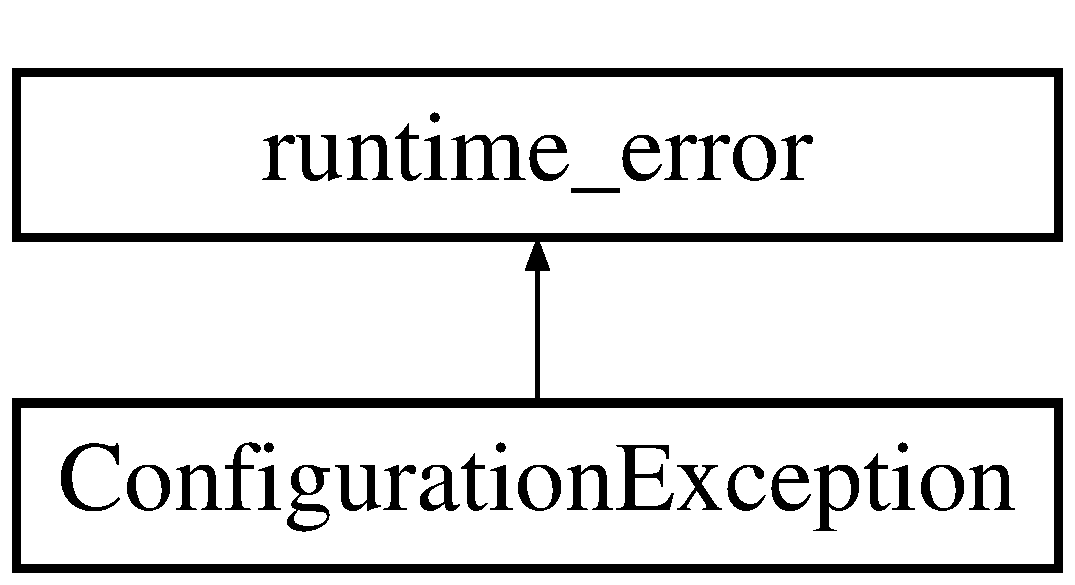
\includegraphics[height=2.000000cm]{class_configuration_exception}
\end{center}
\end{figure}
\subsection*{Public Member Functions}
\begin{DoxyCompactItemize}
\item 
\hyperlink{class_configuration_exception_aafdad5d128d9af78d608ef84bdadefae}{Configuration\+Exception} (const std\+::string \&setting, const std\+::string \&err)
\begin{DoxyCompactList}\small\item\em Default constructor. \end{DoxyCompactList}\item 
const std\+::string \& \hyperlink{class_configuration_exception_abdd1f89e64ba00cf95bf0486f9f79996}{get\+Setting} () const 
\item 
const std\+::string \& \hyperlink{class_configuration_exception_a3977f23c22371c3bc9a9e564afc7778c}{get\+Error} () const 
\end{DoxyCompactItemize}
\subsection*{Protected Attributes}
\begin{DoxyCompactItemize}
\item 
const std\+::string \hyperlink{class_configuration_exception_a5ed87e962e3bb847b29a86b5460b9370}{m\+\_\+\+Setting}
\item 
const std\+::string \hyperlink{class_configuration_exception_a0d142ec503a6f32470c6d262af2d1298}{m\+\_\+\+Error}
\end{DoxyCompactItemize}


\subsection{Detailed Description}
Exception raised whenever a configuration setting is exceptional. 

\begin{DoxyAuthor}{Author}
Hayley Hatton 
\end{DoxyAuthor}
\begin{DoxyDate}{Date}
20/02/2016 
\end{DoxyDate}


Definition at line 12 of file Configuration\+Exception.\+h.



\subsection{Constructor \& Destructor Documentation}
\index{Configuration\+Exception@{Configuration\+Exception}!Configuration\+Exception@{Configuration\+Exception}}
\index{Configuration\+Exception@{Configuration\+Exception}!Configuration\+Exception@{Configuration\+Exception}}
\subsubsection[{\texorpdfstring{Configuration\+Exception(const std\+::string \&setting, const std\+::string \&err)}{ConfigurationException(const std::string &setting, const std::string &err)}}]{\setlength{\rightskip}{0pt plus 5cm}Configuration\+Exception\+::\+Configuration\+Exception (
\begin{DoxyParamCaption}
\item[{const std\+::string \&}]{setting, }
\item[{const std\+::string \&}]{err}
\end{DoxyParamCaption}
)}\hypertarget{class_configuration_exception_aafdad5d128d9af78d608ef84bdadefae}{}\label{class_configuration_exception_aafdad5d128d9af78d608ef84bdadefae}


Default constructor. 


\begin{DoxyParams}{Parameters}
{\em setting} & Configuration setting at fault \\
\hline
{\em err} & Error string \\
\hline
\end{DoxyParams}


Definition at line 3 of file Configuration\+Exception.\+cpp.



\subsection{Member Function Documentation}
\index{Configuration\+Exception@{Configuration\+Exception}!get\+Error@{get\+Error}}
\index{get\+Error@{get\+Error}!Configuration\+Exception@{Configuration\+Exception}}
\subsubsection[{\texorpdfstring{get\+Error() const }{getError() const }}]{\setlength{\rightskip}{0pt plus 5cm}const std\+::string\& Configuration\+Exception\+::get\+Error (
\begin{DoxyParamCaption}
{}
\end{DoxyParamCaption}
) const\hspace{0.3cm}{\ttfamily [inline]}}\hypertarget{class_configuration_exception_a3977f23c22371c3bc9a9e564afc7778c}{}\label{class_configuration_exception_a3977f23c22371c3bc9a9e564afc7778c}


Definition at line 25 of file Configuration\+Exception.\+h.



References m\+\_\+\+Error.



Referenced by Window\+P\+C\+::rendering\+Thread(), and Win\+Main().

\index{Configuration\+Exception@{Configuration\+Exception}!get\+Setting@{get\+Setting}}
\index{get\+Setting@{get\+Setting}!Configuration\+Exception@{Configuration\+Exception}}
\subsubsection[{\texorpdfstring{get\+Setting() const }{getSetting() const }}]{\setlength{\rightskip}{0pt plus 5cm}const std\+::string\& Configuration\+Exception\+::get\+Setting (
\begin{DoxyParamCaption}
{}
\end{DoxyParamCaption}
) const\hspace{0.3cm}{\ttfamily [inline]}}\hypertarget{class_configuration_exception_abdd1f89e64ba00cf95bf0486f9f79996}{}\label{class_configuration_exception_abdd1f89e64ba00cf95bf0486f9f79996}


Definition at line 23 of file Configuration\+Exception.\+h.



References m\+\_\+\+Setting.



Referenced by Window\+P\+C\+::rendering\+Thread(), and Win\+Main().



\subsection{Member Data Documentation}
\index{Configuration\+Exception@{Configuration\+Exception}!m\+\_\+\+Error@{m\+\_\+\+Error}}
\index{m\+\_\+\+Error@{m\+\_\+\+Error}!Configuration\+Exception@{Configuration\+Exception}}
\subsubsection[{\texorpdfstring{m\+\_\+\+Error}{m_Error}}]{\setlength{\rightskip}{0pt plus 5cm}const std\+::string Configuration\+Exception\+::m\+\_\+\+Error\hspace{0.3cm}{\ttfamily [protected]}}\hypertarget{class_configuration_exception_a0d142ec503a6f32470c6d262af2d1298}{}\label{class_configuration_exception_a0d142ec503a6f32470c6d262af2d1298}


Definition at line 29 of file Configuration\+Exception.\+h.



Referenced by get\+Error().

\index{Configuration\+Exception@{Configuration\+Exception}!m\+\_\+\+Setting@{m\+\_\+\+Setting}}
\index{m\+\_\+\+Setting@{m\+\_\+\+Setting}!Configuration\+Exception@{Configuration\+Exception}}
\subsubsection[{\texorpdfstring{m\+\_\+\+Setting}{m_Setting}}]{\setlength{\rightskip}{0pt plus 5cm}const std\+::string Configuration\+Exception\+::m\+\_\+\+Setting\hspace{0.3cm}{\ttfamily [protected]}}\hypertarget{class_configuration_exception_a5ed87e962e3bb847b29a86b5460b9370}{}\label{class_configuration_exception_a5ed87e962e3bb847b29a86b5460b9370}


Definition at line 28 of file Configuration\+Exception.\+h.



Referenced by get\+Setting().



The documentation for this class was generated from the following files\+:\begin{DoxyCompactItemize}
\item 
Lunar\+Drift/engine/exceptions/\hyperlink{_configuration_exception_8h}{Configuration\+Exception.\+h}\item 
Lunar\+Drift/engine/exceptions/\hyperlink{_configuration_exception_8cpp}{Configuration\+Exception.\+cpp}\end{DoxyCompactItemize}

\hypertarget{class_context}{}\section{Context Class Reference}
\label{class_context}\index{Context@{Context}}


Open\+GL context wrapper and provider.  




{\ttfamily \#include $<$Context.\+h$>$}

\subsection*{Public Member Functions}
\begin{DoxyCompactItemize}
\item 
\hyperlink{class_context_a652cdcd2eedc8dbd9110bd284c5d5cf0}{Context} ()
\begin{DoxyCompactList}\small\item\em Default constructor. \end{DoxyCompactList}\item 
virtual \hyperlink{class_context_a2d34e4556448e40693f61d15e091b604}{$\sim$\+Context} ()
\begin{DoxyCompactList}\small\item\em Default destructor. \end{DoxyCompactList}\item 
void \hyperlink{class_context_aa307eab2bab2f1c8fa6f75e507040c67}{set\+Dimensions} (G\+Lsizei width, G\+Lsizei height)
\begin{DoxyCompactList}\small\item\em Set the dimensions of the full rendering context. \end{DoxyCompactList}\item 
void \hyperlink{class_context_a88746b0b9d89b5d7f4e2112440e9bdb3}{get\+Dimensions} (G\+Lsizei $\ast$width, G\+Lsizei $\ast$height) const 
\begin{DoxyCompactList}\small\item\em Access the dimensions of the full rendering context. \end{DoxyCompactList}\end{DoxyCompactItemize}
\subsection*{Private Attributes}
\begin{DoxyCompactItemize}
\item 
G\+Lsizei \hyperlink{class_context_a1813b1a12aaf96ec0ec501194bd56b41}{m\+\_\+\+Width}
\item 
G\+Lsizei \hyperlink{class_context_a78dabc1cab62e8b36ac7330f7c8e4c4b}{m\+\_\+\+Height}
\end{DoxyCompactItemize}


\subsection{Detailed Description}
Open\+GL context wrapper and provider. 

This is practically empty due to the fact Open\+GL\textquotesingle{}s functions and context states are passed around through the thread stack, unlike Direct3D, which has I\+D3\+D11\+Device\+Context and related objects for accessing graphical A\+PI states and calls. However, this should be {\itshape treated} in a similar manner\+: do $<$u$>$not$<$/u$>$ call Open\+GL functions unless a \hyperlink{class_context}{Context} object is present. An exception can be made for Destructors, where parameters cannot be passed in, of course (just be sure to terminate objects on a thread with an Open\+GL context available or Open\+GL delete functions will crash!). Essentially\+: does the function or procedure have a non-\/null \hyperlink{class_context}{Context}? If yes\+: safe to use Open\+GL functions! If no\+: do so at your own risk.

\begin{DoxyAuthor}{Author}
Hayley Hatton 
\end{DoxyAuthor}
\begin{DoxyDate}{Date}
20/02/2016 
\end{DoxyDate}
\begin{DoxySeeAlso}{See also}
\hyperlink{class_renderer}{Renderer} 
\end{DoxySeeAlso}


Definition at line 24 of file Context.\+h.



\subsection{Constructor \& Destructor Documentation}
\index{Context@{Context}!Context@{Context}}
\index{Context@{Context}!Context@{Context}}
\subsubsection[{\texorpdfstring{Context()}{Context()}}]{\setlength{\rightskip}{0pt plus 5cm}Context\+::\+Context (
\begin{DoxyParamCaption}
{}
\end{DoxyParamCaption}
)}\hypertarget{class_context_a652cdcd2eedc8dbd9110bd284c5d5cf0}{}\label{class_context_a652cdcd2eedc8dbd9110bd284c5d5cf0}


Default constructor. 



Definition at line 3 of file Context.\+cpp.

\index{Context@{Context}!````~Context@{$\sim$\+Context}}
\index{````~Context@{$\sim$\+Context}!Context@{Context}}
\subsubsection[{\texorpdfstring{$\sim$\+Context()}{~Context()}}]{\setlength{\rightskip}{0pt plus 5cm}Context\+::$\sim$\+Context (
\begin{DoxyParamCaption}
{}
\end{DoxyParamCaption}
)\hspace{0.3cm}{\ttfamily [virtual]}}\hypertarget{class_context_a2d34e4556448e40693f61d15e091b604}{}\label{class_context_a2d34e4556448e40693f61d15e091b604}


Default destructor. 



Definition at line 8 of file Context.\+cpp.



\subsection{Member Function Documentation}
\index{Context@{Context}!get\+Dimensions@{get\+Dimensions}}
\index{get\+Dimensions@{get\+Dimensions}!Context@{Context}}
\subsubsection[{\texorpdfstring{get\+Dimensions(\+G\+Lsizei $\ast$width, G\+Lsizei $\ast$height) const }{getDimensions(GLsizei *width, GLsizei *height) const }}]{\setlength{\rightskip}{0pt plus 5cm}void Context\+::get\+Dimensions (
\begin{DoxyParamCaption}
\item[{G\+Lsizei $\ast$}]{width, }
\item[{G\+Lsizei $\ast$}]{height}
\end{DoxyParamCaption}
) const}\hypertarget{class_context_a88746b0b9d89b5d7f4e2112440e9bdb3}{}\label{class_context_a88746b0b9d89b5d7f4e2112440e9bdb3}


Access the dimensions of the full rendering context. 


\begin{DoxyParams}{Parameters}
{\em width} & Pointer to store width in pixels \\
\hline
{\em height} & Pointer to store height in pixels \\
\hline
\end{DoxyParams}


Definition at line 20 of file Context.\+cpp.



References m\+\_\+\+Height, and m\+\_\+\+Width.



Referenced by Lunar\+Drift\+Program\+::get\+Renderer(), and Test\+Scene3\+D\+::\+Test\+Scene3\+D().

\index{Context@{Context}!set\+Dimensions@{set\+Dimensions}}
\index{set\+Dimensions@{set\+Dimensions}!Context@{Context}}
\subsubsection[{\texorpdfstring{set\+Dimensions(\+G\+Lsizei width, G\+Lsizei height)}{setDimensions(GLsizei width, GLsizei height)}}]{\setlength{\rightskip}{0pt plus 5cm}void Context\+::set\+Dimensions (
\begin{DoxyParamCaption}
\item[{G\+Lsizei}]{width, }
\item[{G\+Lsizei}]{height}
\end{DoxyParamCaption}
)}\hypertarget{class_context_aa307eab2bab2f1c8fa6f75e507040c67}{}\label{class_context_aa307eab2bab2f1c8fa6f75e507040c67}


Set the dimensions of the full rendering context. 


\begin{DoxyParams}{Parameters}
{\em width} & Width in pixels \\
\hline
{\em height} & Height in pixels \\
\hline
\end{DoxyParams}


Definition at line 14 of file Context.\+cpp.



References m\+\_\+\+Height, and m\+\_\+\+Width.



Referenced by Window\+P\+C\+::create\+Window(), and Window\+P\+C\+::\+Window\+P\+C().



\subsection{Member Data Documentation}
\index{Context@{Context}!m\+\_\+\+Height@{m\+\_\+\+Height}}
\index{m\+\_\+\+Height@{m\+\_\+\+Height}!Context@{Context}}
\subsubsection[{\texorpdfstring{m\+\_\+\+Height}{m_Height}}]{\setlength{\rightskip}{0pt plus 5cm}G\+Lsizei Context\+::m\+\_\+\+Height\hspace{0.3cm}{\ttfamily [private]}}\hypertarget{class_context_a78dabc1cab62e8b36ac7330f7c8e4c4b}{}\label{class_context_a78dabc1cab62e8b36ac7330f7c8e4c4b}


Definition at line 51 of file Context.\+h.



Referenced by get\+Dimensions(), and set\+Dimensions().

\index{Context@{Context}!m\+\_\+\+Width@{m\+\_\+\+Width}}
\index{m\+\_\+\+Width@{m\+\_\+\+Width}!Context@{Context}}
\subsubsection[{\texorpdfstring{m\+\_\+\+Width}{m_Width}}]{\setlength{\rightskip}{0pt plus 5cm}G\+Lsizei Context\+::m\+\_\+\+Width\hspace{0.3cm}{\ttfamily [private]}}\hypertarget{class_context_a1813b1a12aaf96ec0ec501194bd56b41}{}\label{class_context_a1813b1a12aaf96ec0ec501194bd56b41}


Definition at line 51 of file Context.\+h.



Referenced by get\+Dimensions(), and set\+Dimensions().



The documentation for this class was generated from the following files\+:\begin{DoxyCompactItemize}
\item 
Lunar\+Drift/engine/graphics/\hyperlink{_context_8h}{Context.\+h}\item 
Lunar\+Drift/engine/graphics/\hyperlink{_context_8cpp}{Context.\+cpp}\end{DoxyCompactItemize}

\hypertarget{class_controller_button_set}{}\section{Controller\+Button\+Set Class Reference}
\label{class_controller_button_set}\index{Controller\+Button\+Set@{Controller\+Button\+Set}}


{\ttfamily \#include $<$Controller\+Button\+Set.\+h$>$}

\subsection*{Public Member Functions}
\begin{DoxyCompactItemize}
\item 
\hyperlink{class_controller_button_set_ab7b81adc8ef9c94bde050e4d72b208f4}{Controller\+Button\+Set} ()
\item 
virtual \hyperlink{class_controller_button_set_a511e749ae371eed748dbc2ce75e8e5ec}{$\sim$\+Controller\+Button\+Set} ()
\end{DoxyCompactItemize}


\subsection{Detailed Description}


Definition at line 3 of file Controller\+Button\+Set.\+h.



\subsection{Constructor \& Destructor Documentation}
\index{Controller\+Button\+Set@{Controller\+Button\+Set}!Controller\+Button\+Set@{Controller\+Button\+Set}}
\index{Controller\+Button\+Set@{Controller\+Button\+Set}!Controller\+Button\+Set@{Controller\+Button\+Set}}
\subsubsection[{\texorpdfstring{Controller\+Button\+Set()}{ControllerButtonSet()}}]{\setlength{\rightskip}{0pt plus 5cm}Controller\+Button\+Set\+::\+Controller\+Button\+Set (
\begin{DoxyParamCaption}
{}
\end{DoxyParamCaption}
)}\hypertarget{class_controller_button_set_ab7b81adc8ef9c94bde050e4d72b208f4}{}\label{class_controller_button_set_ab7b81adc8ef9c94bde050e4d72b208f4}
Default constructor 

Definition at line 3 of file Controller\+Button\+Set.\+cpp.

\index{Controller\+Button\+Set@{Controller\+Button\+Set}!````~Controller\+Button\+Set@{$\sim$\+Controller\+Button\+Set}}
\index{````~Controller\+Button\+Set@{$\sim$\+Controller\+Button\+Set}!Controller\+Button\+Set@{Controller\+Button\+Set}}
\subsubsection[{\texorpdfstring{$\sim$\+Controller\+Button\+Set()}{~ControllerButtonSet()}}]{\setlength{\rightskip}{0pt plus 5cm}Controller\+Button\+Set\+::$\sim$\+Controller\+Button\+Set (
\begin{DoxyParamCaption}
{}
\end{DoxyParamCaption}
)\hspace{0.3cm}{\ttfamily [virtual]}}\hypertarget{class_controller_button_set_a511e749ae371eed748dbc2ce75e8e5ec}{}\label{class_controller_button_set_a511e749ae371eed748dbc2ce75e8e5ec}
Default destructor 

Definition at line 8 of file Controller\+Button\+Set.\+cpp.



The documentation for this class was generated from the following files\+:\begin{DoxyCompactItemize}
\item 
Lunar\+Drift/engine/input/\hyperlink{_controller_button_set_8h}{Controller\+Button\+Set.\+h}\item 
Lunar\+Drift/engine/input/\hyperlink{_controller_button_set_8cpp}{Controller\+Button\+Set.\+cpp}\end{DoxyCompactItemize}

\hypertarget{class_damage_message}{}\section{Damage\+Message Class Reference}
\label{class_damage_message}\index{Damage\+Message@{Damage\+Message}}


{\ttfamily \#include $<$Damage\+Message.\+h$>$}

Inheritance diagram for Damage\+Message\+:\begin{figure}[H]
\begin{center}
\leavevmode
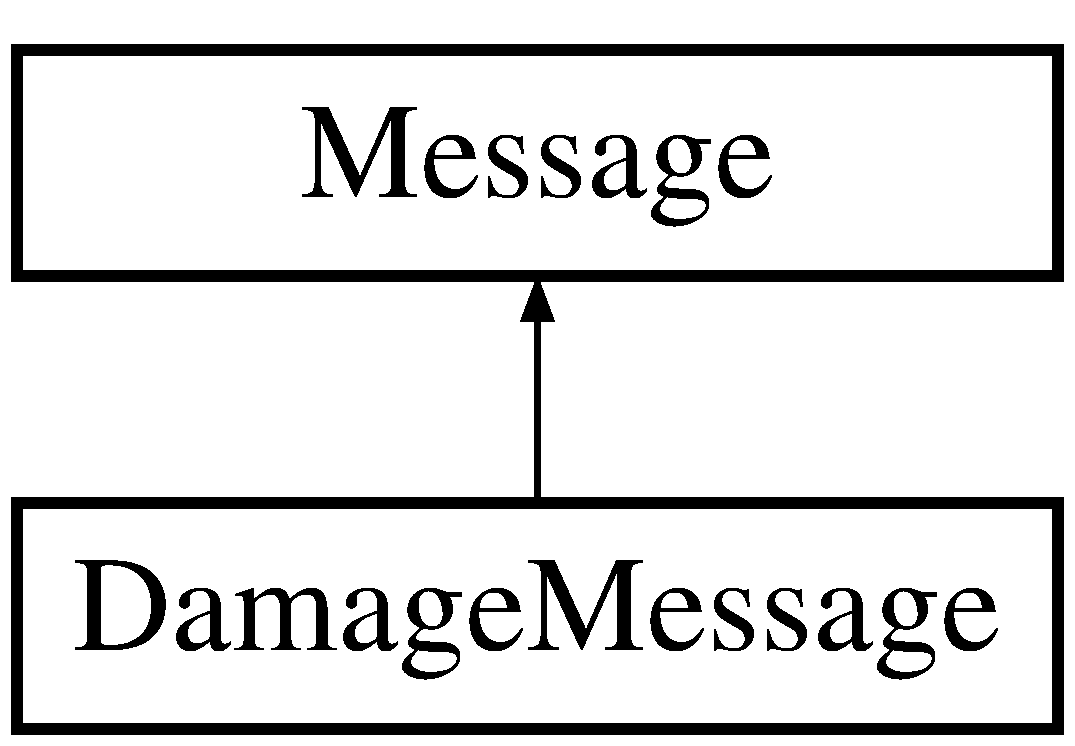
\includegraphics[height=2.000000cm]{class_damage_message}
\end{center}
\end{figure}
\subsection*{Public Member Functions}
\begin{DoxyCompactItemize}
\item 
\hyperlink{class_damage_message_a26d1bff48f200de36e3401133026c94a}{Damage\+Message} (\hyperlink{class_scene_object}{Scene\+Object} $\ast$target, int damage, \hyperlink{class_scene_object}{Scene\+Object} $\ast$source=nullptr)
\item 
virtual \hyperlink{class_damage_message_a0fffc9a2df40368c8ac11b34078d5067}{$\sim$\+Damage\+Message} ()
\item 
\hyperlink{class_scene_object}{Scene\+Object} $\ast$ \hyperlink{class_damage_message_a10fd1ad5f3ca88a6c0d75bfa7a65db8b}{get\+Target} ()
\item 
\hyperlink{class_scene_object}{Scene\+Object} $\ast$ \hyperlink{class_damage_message_a2bacfef6bb9a3862abf968a8fc704724}{get\+Source} ()
\item 
int \hyperlink{class_damage_message_a5d7f2a29ad64c0f8650866827f6281bf}{get\+Damage} () const 
\end{DoxyCompactItemize}
\subsection*{Private Attributes}
\begin{DoxyCompactItemize}
\item 
\hyperlink{class_scene_object}{Scene\+Object} $\ast$ \hyperlink{class_damage_message_aa0b42b74f7243b8636d4b4b467f76d8e}{m\+\_\+\+Target}
\item 
\hyperlink{class_scene_object}{Scene\+Object} $\ast$ \hyperlink{class_damage_message_a6b0e3e9316ba34f864e93fa73b8cba67}{m\+\_\+\+Source}
\item 
int \hyperlink{class_damage_message_a13210e9d91fcac17df553f1f3d029275}{m\+\_\+\+Damage}
\end{DoxyCompactItemize}


\subsection{Detailed Description}


Definition at line 6 of file Damage\+Message.\+h.



\subsection{Constructor \& Destructor Documentation}
\index{Damage\+Message@{Damage\+Message}!Damage\+Message@{Damage\+Message}}
\index{Damage\+Message@{Damage\+Message}!Damage\+Message@{Damage\+Message}}
\subsubsection[{\texorpdfstring{Damage\+Message(\+Scene\+Object $\ast$target, int damage, Scene\+Object $\ast$source=nullptr)}{DamageMessage(SceneObject *target, int damage, SceneObject *source=nullptr)}}]{\setlength{\rightskip}{0pt plus 5cm}Damage\+Message\+::\+Damage\+Message (
\begin{DoxyParamCaption}
\item[{{\bf Scene\+Object} $\ast$}]{target, }
\item[{int}]{damage, }
\item[{{\bf Scene\+Object} $\ast$}]{source = {\ttfamily nullptr}}
\end{DoxyParamCaption}
)}\hypertarget{class_damage_message_a26d1bff48f200de36e3401133026c94a}{}\label{class_damage_message_a26d1bff48f200de36e3401133026c94a}


Definition at line 4 of file Damage\+Message.\+cpp.

\index{Damage\+Message@{Damage\+Message}!````~Damage\+Message@{$\sim$\+Damage\+Message}}
\index{````~Damage\+Message@{$\sim$\+Damage\+Message}!Damage\+Message@{Damage\+Message}}
\subsubsection[{\texorpdfstring{$\sim$\+Damage\+Message()}{~DamageMessage()}}]{\setlength{\rightskip}{0pt plus 5cm}Damage\+Message\+::$\sim$\+Damage\+Message (
\begin{DoxyParamCaption}
{}
\end{DoxyParamCaption}
)\hspace{0.3cm}{\ttfamily [virtual]}}\hypertarget{class_damage_message_a0fffc9a2df40368c8ac11b34078d5067}{}\label{class_damage_message_a0fffc9a2df40368c8ac11b34078d5067}


Definition at line 15 of file Damage\+Message.\+cpp.



\subsection{Member Function Documentation}
\index{Damage\+Message@{Damage\+Message}!get\+Damage@{get\+Damage}}
\index{get\+Damage@{get\+Damage}!Damage\+Message@{Damage\+Message}}
\subsubsection[{\texorpdfstring{get\+Damage() const }{getDamage() const }}]{\setlength{\rightskip}{0pt plus 5cm}int Damage\+Message\+::get\+Damage (
\begin{DoxyParamCaption}
{}
\end{DoxyParamCaption}
) const\hspace{0.3cm}{\ttfamily [inline]}}\hypertarget{class_damage_message_a5d7f2a29ad64c0f8650866827f6281bf}{}\label{class_damage_message_a5d7f2a29ad64c0f8650866827f6281bf}


Definition at line 22 of file Damage\+Message.\+h.



References m\+\_\+\+Damage.

\index{Damage\+Message@{Damage\+Message}!get\+Source@{get\+Source}}
\index{get\+Source@{get\+Source}!Damage\+Message@{Damage\+Message}}
\subsubsection[{\texorpdfstring{get\+Source()}{getSource()}}]{\setlength{\rightskip}{0pt plus 5cm}{\bf Scene\+Object}$\ast$ Damage\+Message\+::get\+Source (
\begin{DoxyParamCaption}
{}
\end{DoxyParamCaption}
)\hspace{0.3cm}{\ttfamily [inline]}}\hypertarget{class_damage_message_a2bacfef6bb9a3862abf968a8fc704724}{}\label{class_damage_message_a2bacfef6bb9a3862abf968a8fc704724}


Definition at line 20 of file Damage\+Message.\+h.



References m\+\_\+\+Source.

\index{Damage\+Message@{Damage\+Message}!get\+Target@{get\+Target}}
\index{get\+Target@{get\+Target}!Damage\+Message@{Damage\+Message}}
\subsubsection[{\texorpdfstring{get\+Target()}{getTarget()}}]{\setlength{\rightskip}{0pt plus 5cm}{\bf Scene\+Object}$\ast$ Damage\+Message\+::get\+Target (
\begin{DoxyParamCaption}
{}
\end{DoxyParamCaption}
)\hspace{0.3cm}{\ttfamily [inline]}}\hypertarget{class_damage_message_a10fd1ad5f3ca88a6c0d75bfa7a65db8b}{}\label{class_damage_message_a10fd1ad5f3ca88a6c0d75bfa7a65db8b}


Definition at line 18 of file Damage\+Message.\+h.



References m\+\_\+\+Target.



\subsection{Member Data Documentation}
\index{Damage\+Message@{Damage\+Message}!m\+\_\+\+Damage@{m\+\_\+\+Damage}}
\index{m\+\_\+\+Damage@{m\+\_\+\+Damage}!Damage\+Message@{Damage\+Message}}
\subsubsection[{\texorpdfstring{m\+\_\+\+Damage}{m_Damage}}]{\setlength{\rightskip}{0pt plus 5cm}int Damage\+Message\+::m\+\_\+\+Damage\hspace{0.3cm}{\ttfamily [private]}}\hypertarget{class_damage_message_a13210e9d91fcac17df553f1f3d029275}{}\label{class_damage_message_a13210e9d91fcac17df553f1f3d029275}


Definition at line 27 of file Damage\+Message.\+h.



Referenced by get\+Damage().

\index{Damage\+Message@{Damage\+Message}!m\+\_\+\+Source@{m\+\_\+\+Source}}
\index{m\+\_\+\+Source@{m\+\_\+\+Source}!Damage\+Message@{Damage\+Message}}
\subsubsection[{\texorpdfstring{m\+\_\+\+Source}{m_Source}}]{\setlength{\rightskip}{0pt plus 5cm}{\bf Scene\+Object}$\ast$ Damage\+Message\+::m\+\_\+\+Source\hspace{0.3cm}{\ttfamily [private]}}\hypertarget{class_damage_message_a6b0e3e9316ba34f864e93fa73b8cba67}{}\label{class_damage_message_a6b0e3e9316ba34f864e93fa73b8cba67}


Definition at line 26 of file Damage\+Message.\+h.



Referenced by get\+Source().

\index{Damage\+Message@{Damage\+Message}!m\+\_\+\+Target@{m\+\_\+\+Target}}
\index{m\+\_\+\+Target@{m\+\_\+\+Target}!Damage\+Message@{Damage\+Message}}
\subsubsection[{\texorpdfstring{m\+\_\+\+Target}{m_Target}}]{\setlength{\rightskip}{0pt plus 5cm}{\bf Scene\+Object}$\ast$ Damage\+Message\+::m\+\_\+\+Target\hspace{0.3cm}{\ttfamily [private]}}\hypertarget{class_damage_message_aa0b42b74f7243b8636d4b4b467f76d8e}{}\label{class_damage_message_aa0b42b74f7243b8636d4b4b467f76d8e}


Definition at line 25 of file Damage\+Message.\+h.



Referenced by get\+Target().



The documentation for this class was generated from the following files\+:\begin{DoxyCompactItemize}
\item 
Lunar\+Drift/engine/comms/predefined/\hyperlink{_damage_message_8h}{Damage\+Message.\+h}\item 
Lunar\+Drift/engine/comms/predefined/\hyperlink{_damage_message_8cpp}{Damage\+Message.\+cpp}\end{DoxyCompactItemize}

\hypertarget{class_death_message}{}\section{Death\+Message Class Reference}
\label{class_death_message}\index{Death\+Message@{Death\+Message}}


{\ttfamily \#include $<$Death\+Message.\+h$>$}

Inheritance diagram for Death\+Message\+:\begin{figure}[H]
\begin{center}
\leavevmode
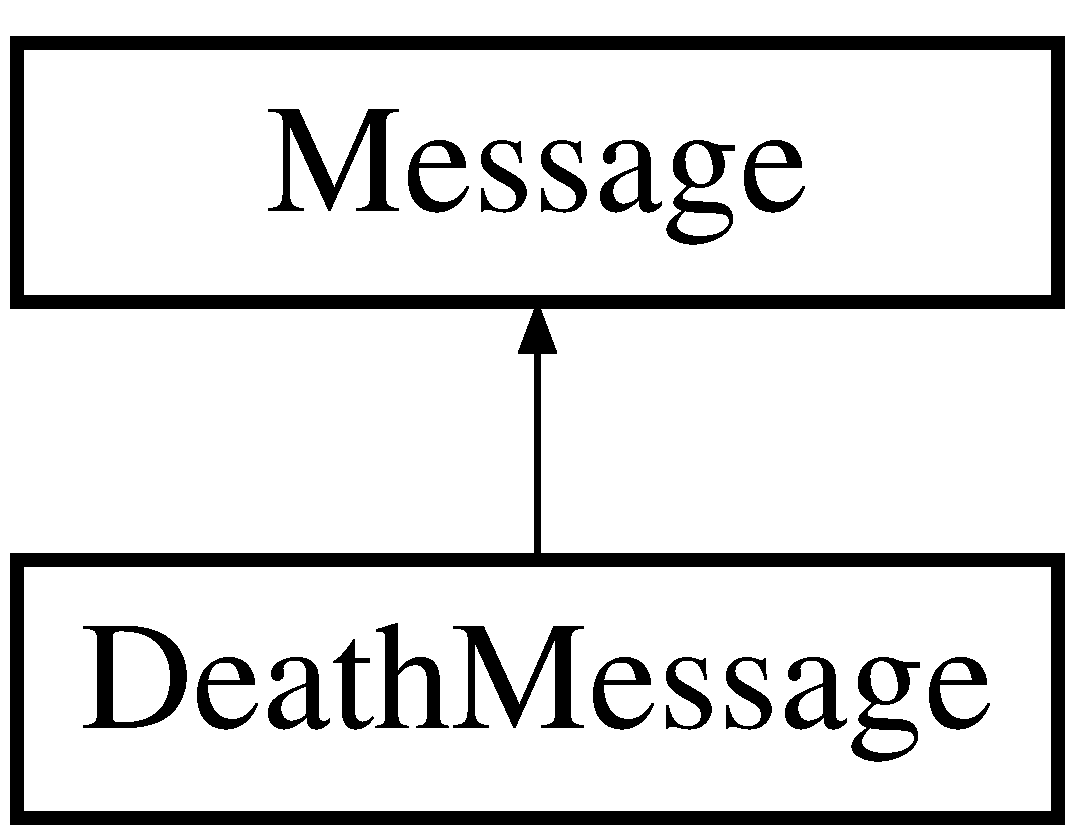
\includegraphics[height=2.000000cm]{class_death_message}
\end{center}
\end{figure}
\subsection*{Public Member Functions}
\begin{DoxyCompactItemize}
\item 
\hyperlink{class_death_message_a921f4cad06cfdd3027128d4a7c9e6337}{Death\+Message} (\hyperlink{class_scene_object}{Scene\+Object} $\ast$doomed, \hyperlink{class_scene_object}{Scene\+Object} $\ast$killer=nullptr)
\item 
\hyperlink{class_death_message_a90e7cb9fe52f52a5d968f95683e0a740}{$\sim$\+Death\+Message} ()
\item 
\hyperlink{class_scene_object}{Scene\+Object} $\ast$ \hyperlink{class_death_message_a3a8862fc0961077bc45345f56aa1c9ce}{get\+Doomed} () const 
\item 
\hyperlink{class_scene_object}{Scene\+Object} $\ast$ \hyperlink{class_death_message_a0451c68fe223c3d13e4d4e3c4c55bf8e}{get\+Killer} () const 
\end{DoxyCompactItemize}
\subsection*{Private Attributes}
\begin{DoxyCompactItemize}
\item 
\hyperlink{class_scene_object}{Scene\+Object} $\ast$ \hyperlink{class_death_message_a34cafaafa984ec952e2cb23dc5de64b5}{m\+\_\+\+Doomed}
\item 
\hyperlink{class_scene_object}{Scene\+Object} $\ast$ \hyperlink{class_death_message_a34e6b366368536231d282a6934042b73}{m\+\_\+\+Killer}
\end{DoxyCompactItemize}


\subsection{Detailed Description}


Definition at line 6 of file Death\+Message.\+h.



\subsection{Constructor \& Destructor Documentation}
\index{Death\+Message@{Death\+Message}!Death\+Message@{Death\+Message}}
\index{Death\+Message@{Death\+Message}!Death\+Message@{Death\+Message}}
\subsubsection[{\texorpdfstring{Death\+Message(\+Scene\+Object $\ast$doomed, Scene\+Object $\ast$killer=nullptr)}{DeathMessage(SceneObject *doomed, SceneObject *killer=nullptr)}}]{\setlength{\rightskip}{0pt plus 5cm}Death\+Message\+::\+Death\+Message (
\begin{DoxyParamCaption}
\item[{{\bf Scene\+Object} $\ast$}]{doomed, }
\item[{{\bf Scene\+Object} $\ast$}]{killer = {\ttfamily nullptr}}
\end{DoxyParamCaption}
)}\hypertarget{class_death_message_a921f4cad06cfdd3027128d4a7c9e6337}{}\label{class_death_message_a921f4cad06cfdd3027128d4a7c9e6337}


Definition at line 4 of file Death\+Message.\+cpp.

\index{Death\+Message@{Death\+Message}!````~Death\+Message@{$\sim$\+Death\+Message}}
\index{````~Death\+Message@{$\sim$\+Death\+Message}!Death\+Message@{Death\+Message}}
\subsubsection[{\texorpdfstring{$\sim$\+Death\+Message()}{~DeathMessage()}}]{\setlength{\rightskip}{0pt plus 5cm}Death\+Message\+::$\sim$\+Death\+Message (
\begin{DoxyParamCaption}
{}
\end{DoxyParamCaption}
)}\hypertarget{class_death_message_a90e7cb9fe52f52a5d968f95683e0a740}{}\label{class_death_message_a90e7cb9fe52f52a5d968f95683e0a740}


Definition at line 11 of file Death\+Message.\+cpp.



\subsection{Member Function Documentation}
\index{Death\+Message@{Death\+Message}!get\+Doomed@{get\+Doomed}}
\index{get\+Doomed@{get\+Doomed}!Death\+Message@{Death\+Message}}
\subsubsection[{\texorpdfstring{get\+Doomed() const }{getDoomed() const }}]{\setlength{\rightskip}{0pt plus 5cm}{\bf Scene\+Object}$\ast$ Death\+Message\+::get\+Doomed (
\begin{DoxyParamCaption}
{}
\end{DoxyParamCaption}
) const\hspace{0.3cm}{\ttfamily [inline]}}\hypertarget{class_death_message_a3a8862fc0961077bc45345f56aa1c9ce}{}\label{class_death_message_a3a8862fc0961077bc45345f56aa1c9ce}


Definition at line 14 of file Death\+Message.\+h.



References m\+\_\+\+Doomed.

\index{Death\+Message@{Death\+Message}!get\+Killer@{get\+Killer}}
\index{get\+Killer@{get\+Killer}!Death\+Message@{Death\+Message}}
\subsubsection[{\texorpdfstring{get\+Killer() const }{getKiller() const }}]{\setlength{\rightskip}{0pt plus 5cm}{\bf Scene\+Object}$\ast$ Death\+Message\+::get\+Killer (
\begin{DoxyParamCaption}
{}
\end{DoxyParamCaption}
) const\hspace{0.3cm}{\ttfamily [inline]}}\hypertarget{class_death_message_a0451c68fe223c3d13e4d4e3c4c55bf8e}{}\label{class_death_message_a0451c68fe223c3d13e4d4e3c4c55bf8e}


Definition at line 16 of file Death\+Message.\+h.



References m\+\_\+\+Killer.



\subsection{Member Data Documentation}
\index{Death\+Message@{Death\+Message}!m\+\_\+\+Doomed@{m\+\_\+\+Doomed}}
\index{m\+\_\+\+Doomed@{m\+\_\+\+Doomed}!Death\+Message@{Death\+Message}}
\subsubsection[{\texorpdfstring{m\+\_\+\+Doomed}{m_Doomed}}]{\setlength{\rightskip}{0pt plus 5cm}{\bf Scene\+Object}$\ast$ Death\+Message\+::m\+\_\+\+Doomed\hspace{0.3cm}{\ttfamily [private]}}\hypertarget{class_death_message_a34cafaafa984ec952e2cb23dc5de64b5}{}\label{class_death_message_a34cafaafa984ec952e2cb23dc5de64b5}


Definition at line 19 of file Death\+Message.\+h.



Referenced by get\+Doomed().

\index{Death\+Message@{Death\+Message}!m\+\_\+\+Killer@{m\+\_\+\+Killer}}
\index{m\+\_\+\+Killer@{m\+\_\+\+Killer}!Death\+Message@{Death\+Message}}
\subsubsection[{\texorpdfstring{m\+\_\+\+Killer}{m_Killer}}]{\setlength{\rightskip}{0pt plus 5cm}{\bf Scene\+Object}$\ast$ Death\+Message\+::m\+\_\+\+Killer\hspace{0.3cm}{\ttfamily [private]}}\hypertarget{class_death_message_a34e6b366368536231d282a6934042b73}{}\label{class_death_message_a34e6b366368536231d282a6934042b73}


Definition at line 20 of file Death\+Message.\+h.



Referenced by get\+Killer().



The documentation for this class was generated from the following files\+:\begin{DoxyCompactItemize}
\item 
Lunar\+Drift/engine/comms/predefined/\hyperlink{_death_message_8h}{Death\+Message.\+h}\item 
Lunar\+Drift/engine/comms/predefined/\hyperlink{_death_message_8cpp}{Death\+Message.\+cpp}\end{DoxyCompactItemize}

\hypertarget{class_file_i_o_exception}{}\section{File\+I\+O\+Exception Class Reference}
\label{class_file_i_o_exception}\index{File\+I\+O\+Exception@{File\+I\+O\+Exception}}


Exception raised whenever a core filesystem operation fails.  




{\ttfamily \#include $<$File\+I\+O\+Exception.\+h$>$}

Inheritance diagram for File\+I\+O\+Exception\+:\begin{figure}[H]
\begin{center}
\leavevmode
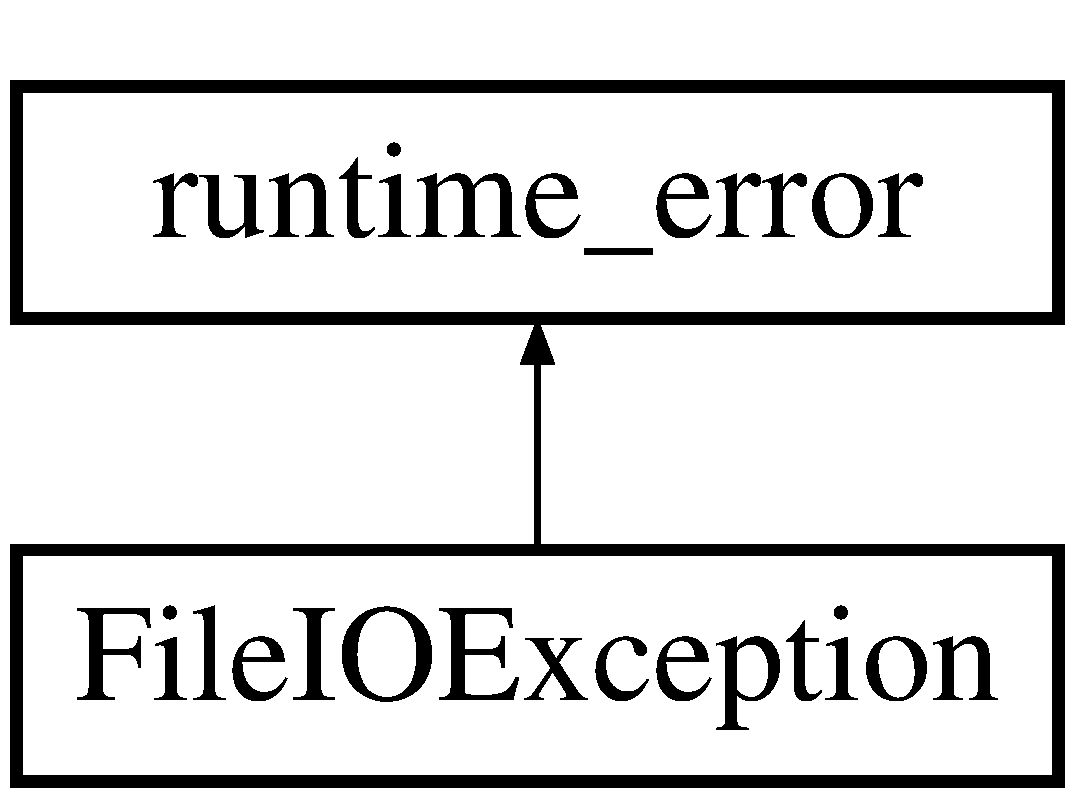
\includegraphics[height=2.000000cm]{class_file_i_o_exception}
\end{center}
\end{figure}
\subsection*{Public Member Functions}
\begin{DoxyCompactItemize}
\item 
\hyperlink{class_file_i_o_exception_a50807e035fd588fdba672b626e7e950a}{File\+I\+O\+Exception} (const std\+::string \&file, const std\+::string \&err)
\begin{DoxyCompactList}\small\item\em Default constructor. \end{DoxyCompactList}\item 
const std\+::string \& \hyperlink{class_file_i_o_exception_afb4ef7ef699df309bb14cc97cb3f52ed}{get\+File} () const 
\item 
const std\+::string \& \hyperlink{class_file_i_o_exception_a8230811beaad6b8352f972f616f51d09}{get\+Error} () const 
\end{DoxyCompactItemize}
\subsection*{Private Attributes}
\begin{DoxyCompactItemize}
\item 
const std\+::string \hyperlink{class_file_i_o_exception_aabe82501c1620dae2236fe2c877c36ed}{m\+\_\+\+File}
\item 
const std\+::string \hyperlink{class_file_i_o_exception_a2f1715571b72f01da492e6d2429f7a29}{m\+\_\+\+Error}
\end{DoxyCompactItemize}


\subsection{Detailed Description}
Exception raised whenever a core filesystem operation fails. 

\begin{DoxyAuthor}{Author}
Hayley Hatton 
\end{DoxyAuthor}
\begin{DoxyDate}{Date}
20/02/2016 
\end{DoxyDate}


Definition at line 12 of file File\+I\+O\+Exception.\+h.



\subsection{Constructor \& Destructor Documentation}
\index{File\+I\+O\+Exception@{File\+I\+O\+Exception}!File\+I\+O\+Exception@{File\+I\+O\+Exception}}
\index{File\+I\+O\+Exception@{File\+I\+O\+Exception}!File\+I\+O\+Exception@{File\+I\+O\+Exception}}
\subsubsection[{\texorpdfstring{File\+I\+O\+Exception(const std\+::string \&file, const std\+::string \&err)}{FileIOException(const std::string &file, const std::string &err)}}]{\setlength{\rightskip}{0pt plus 5cm}File\+I\+O\+Exception\+::\+File\+I\+O\+Exception (
\begin{DoxyParamCaption}
\item[{const std\+::string \&}]{file, }
\item[{const std\+::string \&}]{err}
\end{DoxyParamCaption}
)}\hypertarget{class_file_i_o_exception_a50807e035fd588fdba672b626e7e950a}{}\label{class_file_i_o_exception_a50807e035fd588fdba672b626e7e950a}


Default constructor. 


\begin{DoxyParams}{Parameters}
{\em file} & File name of the failed file. \\
\hline
{\em err} & Error string \\
\hline
\end{DoxyParams}


Definition at line 3 of file File\+I\+O\+Exception.\+cpp.



\subsection{Member Function Documentation}
\index{File\+I\+O\+Exception@{File\+I\+O\+Exception}!get\+Error@{get\+Error}}
\index{get\+Error@{get\+Error}!File\+I\+O\+Exception@{File\+I\+O\+Exception}}
\subsubsection[{\texorpdfstring{get\+Error() const }{getError() const }}]{\setlength{\rightskip}{0pt plus 5cm}const std\+::string\& File\+I\+O\+Exception\+::get\+Error (
\begin{DoxyParamCaption}
{}
\end{DoxyParamCaption}
) const\hspace{0.3cm}{\ttfamily [inline]}}\hypertarget{class_file_i_o_exception_a8230811beaad6b8352f972f616f51d09}{}\label{class_file_i_o_exception_a8230811beaad6b8352f972f616f51d09}


Definition at line 26 of file File\+I\+O\+Exception.\+h.



References m\+\_\+\+Error.



Referenced by Window\+P\+C\+::rendering\+Thread(), and Win\+Main().

\index{File\+I\+O\+Exception@{File\+I\+O\+Exception}!get\+File@{get\+File}}
\index{get\+File@{get\+File}!File\+I\+O\+Exception@{File\+I\+O\+Exception}}
\subsubsection[{\texorpdfstring{get\+File() const }{getFile() const }}]{\setlength{\rightskip}{0pt plus 5cm}const std\+::string\& File\+I\+O\+Exception\+::get\+File (
\begin{DoxyParamCaption}
{}
\end{DoxyParamCaption}
) const\hspace{0.3cm}{\ttfamily [inline]}}\hypertarget{class_file_i_o_exception_afb4ef7ef699df309bb14cc97cb3f52ed}{}\label{class_file_i_o_exception_afb4ef7ef699df309bb14cc97cb3f52ed}


Definition at line 24 of file File\+I\+O\+Exception.\+h.



References m\+\_\+\+File.



Referenced by Window\+P\+C\+::rendering\+Thread(), and Win\+Main().



\subsection{Member Data Documentation}
\index{File\+I\+O\+Exception@{File\+I\+O\+Exception}!m\+\_\+\+Error@{m\+\_\+\+Error}}
\index{m\+\_\+\+Error@{m\+\_\+\+Error}!File\+I\+O\+Exception@{File\+I\+O\+Exception}}
\subsubsection[{\texorpdfstring{m\+\_\+\+Error}{m_Error}}]{\setlength{\rightskip}{0pt plus 5cm}const std\+::string File\+I\+O\+Exception\+::m\+\_\+\+Error\hspace{0.3cm}{\ttfamily [private]}}\hypertarget{class_file_i_o_exception_a2f1715571b72f01da492e6d2429f7a29}{}\label{class_file_i_o_exception_a2f1715571b72f01da492e6d2429f7a29}


Definition at line 30 of file File\+I\+O\+Exception.\+h.



Referenced by get\+Error().

\index{File\+I\+O\+Exception@{File\+I\+O\+Exception}!m\+\_\+\+File@{m\+\_\+\+File}}
\index{m\+\_\+\+File@{m\+\_\+\+File}!File\+I\+O\+Exception@{File\+I\+O\+Exception}}
\subsubsection[{\texorpdfstring{m\+\_\+\+File}{m_File}}]{\setlength{\rightskip}{0pt plus 5cm}const std\+::string File\+I\+O\+Exception\+::m\+\_\+\+File\hspace{0.3cm}{\ttfamily [private]}}\hypertarget{class_file_i_o_exception_aabe82501c1620dae2236fe2c877c36ed}{}\label{class_file_i_o_exception_aabe82501c1620dae2236fe2c877c36ed}


Definition at line 29 of file File\+I\+O\+Exception.\+h.



Referenced by get\+File().



The documentation for this class was generated from the following files\+:\begin{DoxyCompactItemize}
\item 
Lunar\+Drift/engine/exceptions/\hyperlink{_file_i_o_exception_8h}{File\+I\+O\+Exception.\+h}\item 
Lunar\+Drift/engine/exceptions/\hyperlink{_file_i_o_exception_8cpp}{File\+I\+O\+Exception.\+cpp}\end{DoxyCompactItemize}

\hypertarget{class_framebuffer}{}\section{Framebuffer Class Reference}
\label{class_framebuffer}\index{Framebuffer@{Framebuffer}}


{\ttfamily \#include $<$Framebuffer.\+h$>$}

\subsection*{Public Member Functions}
\begin{DoxyCompactItemize}
\item 
\hyperlink{class_framebuffer_a4f10f2020d414add1ea0e6553908c86b}{Framebuffer} ()
\item 
virtual \hyperlink{class_framebuffer_a037bf3e17455354d5d907ceea00313dd}{$\sim$\+Framebuffer} ()
\end{DoxyCompactItemize}


\subsection{Detailed Description}


Definition at line 3 of file Framebuffer.\+h.



\subsection{Constructor \& Destructor Documentation}
\index{Framebuffer@{Framebuffer}!Framebuffer@{Framebuffer}}
\index{Framebuffer@{Framebuffer}!Framebuffer@{Framebuffer}}
\subsubsection[{\texorpdfstring{Framebuffer()}{Framebuffer()}}]{\setlength{\rightskip}{0pt plus 5cm}Framebuffer\+::\+Framebuffer (
\begin{DoxyParamCaption}
{}
\end{DoxyParamCaption}
)}\hypertarget{class_framebuffer_a4f10f2020d414add1ea0e6553908c86b}{}\label{class_framebuffer_a4f10f2020d414add1ea0e6553908c86b}
Default constructor 

Definition at line 3 of file Framebuffer.\+cpp.

\index{Framebuffer@{Framebuffer}!````~Framebuffer@{$\sim$\+Framebuffer}}
\index{````~Framebuffer@{$\sim$\+Framebuffer}!Framebuffer@{Framebuffer}}
\subsubsection[{\texorpdfstring{$\sim$\+Framebuffer()}{~Framebuffer()}}]{\setlength{\rightskip}{0pt plus 5cm}Framebuffer\+::$\sim$\+Framebuffer (
\begin{DoxyParamCaption}
{}
\end{DoxyParamCaption}
)\hspace{0.3cm}{\ttfamily [virtual]}}\hypertarget{class_framebuffer_a037bf3e17455354d5d907ceea00313dd}{}\label{class_framebuffer_a037bf3e17455354d5d907ceea00313dd}
Default destructor 

Definition at line 8 of file Framebuffer.\+cpp.



The documentation for this class was generated from the following files\+:\begin{DoxyCompactItemize}
\item 
Lunar\+Drift/engine/graphics/\hyperlink{_framebuffer_8h}{Framebuffer.\+h}\item 
Lunar\+Drift/engine/graphics/\hyperlink{_framebuffer_8cpp}{Framebuffer.\+cpp}\end{DoxyCompactItemize}

\hypertarget{class_game_renderer}{}\section{Game\+Renderer Class Reference}
\label{class_game_renderer}\index{Game\+Renderer@{Game\+Renderer}}


{\ttfamily \#include $<$Game\+Renderer.\+h$>$}

Inheritance diagram for Game\+Renderer\+:\begin{figure}[H]
\begin{center}
\leavevmode
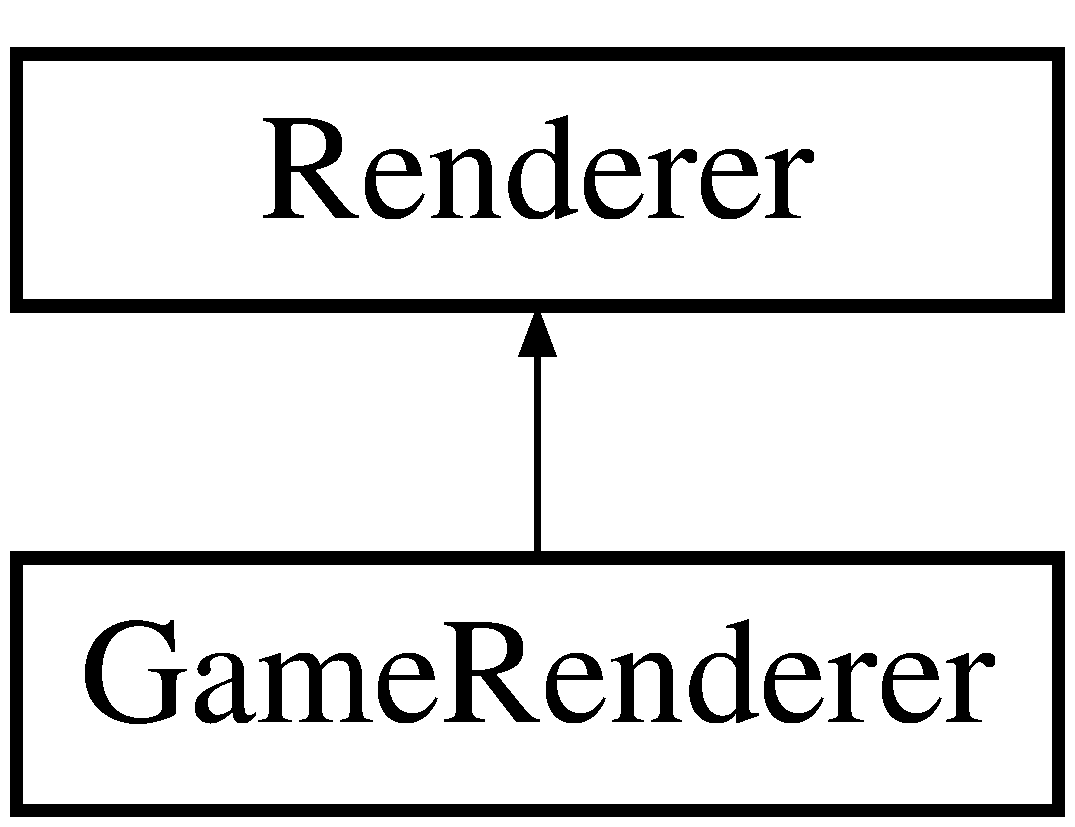
\includegraphics[height=2.000000cm]{class_game_renderer}
\end{center}
\end{figure}
\subsection*{Public Member Functions}
\begin{DoxyCompactItemize}
\item 
\hyperlink{class_game_renderer_a91d4feda47647fc97397d9e09bbc36df}{Game\+Renderer} (\hyperlink{class_context}{Context} $\ast$context, G\+Lsizei width, G\+Lsizei height)
\begin{DoxyCompactList}\small\item\em Default constructor. \end{DoxyCompactList}\item 
\hyperlink{class_game_renderer_a7548becdb4364d14cafa7a5436f42af6}{$\sim$\+Game\+Renderer} ()
\begin{DoxyCompactList}\small\item\em Default destructor. \end{DoxyCompactList}\end{DoxyCompactItemize}
\subsection*{Protected Member Functions}
\begin{DoxyCompactItemize}
\item 
std\+::shared\+\_\+ptr$<$ \hyperlink{class_shader_manager}{Shader\+Manager} $>$ \hyperlink{class_game_renderer_ac01f6745a9dd800dfe4c5fb12d46bc38}{load\+Standard\+Shaders} (\hyperlink{class_context}{Context} $\ast$context) override
\begin{DoxyCompactList}\small\item\em Create and return a shader manager containing the standard shaders. \end{DoxyCompactList}\end{DoxyCompactItemize}


\subsection{Detailed Description}


Definition at line 5 of file Game\+Renderer.\+h.



\subsection{Constructor \& Destructor Documentation}
\index{Game\+Renderer@{Game\+Renderer}!Game\+Renderer@{Game\+Renderer}}
\index{Game\+Renderer@{Game\+Renderer}!Game\+Renderer@{Game\+Renderer}}
\subsubsection[{\texorpdfstring{Game\+Renderer(\+Context $\ast$context, G\+Lsizei width, G\+Lsizei height)}{GameRenderer(Context *context, GLsizei width, GLsizei height)}}]{\setlength{\rightskip}{0pt plus 5cm}Game\+Renderer\+::\+Game\+Renderer (
\begin{DoxyParamCaption}
\item[{{\bf Context} $\ast$}]{context, }
\item[{G\+Lsizei}]{width, }
\item[{G\+Lsizei}]{height}
\end{DoxyParamCaption}
)}\hypertarget{class_game_renderer_a91d4feda47647fc97397d9e09bbc36df}{}\label{class_game_renderer_a91d4feda47647fc97397d9e09bbc36df}


Default constructor. 


\begin{DoxyParams}{Parameters}
{\em context} & Graphics context \\
\hline
{\em width} & Width of context in pixels \\
\hline
{\em height} & Height of context in pixels \\
\hline
\end{DoxyParams}


Definition at line 3 of file Game\+Renderer.\+cpp.



References f, Renderer\+::load(), and Renderer\+::set\+Clear\+Color().

\index{Game\+Renderer@{Game\+Renderer}!````~Game\+Renderer@{$\sim$\+Game\+Renderer}}
\index{````~Game\+Renderer@{$\sim$\+Game\+Renderer}!Game\+Renderer@{Game\+Renderer}}
\subsubsection[{\texorpdfstring{$\sim$\+Game\+Renderer()}{~GameRenderer()}}]{\setlength{\rightskip}{0pt plus 5cm}Game\+Renderer\+::$\sim$\+Game\+Renderer (
\begin{DoxyParamCaption}
{}
\end{DoxyParamCaption}
)}\hypertarget{class_game_renderer_a7548becdb4364d14cafa7a5436f42af6}{}\label{class_game_renderer_a7548becdb4364d14cafa7a5436f42af6}


Default destructor. 



Definition at line 12 of file Game\+Renderer.\+cpp.



\subsection{Member Function Documentation}
\index{Game\+Renderer@{Game\+Renderer}!load\+Standard\+Shaders@{load\+Standard\+Shaders}}
\index{load\+Standard\+Shaders@{load\+Standard\+Shaders}!Game\+Renderer@{Game\+Renderer}}
\subsubsection[{\texorpdfstring{load\+Standard\+Shaders(\+Context $\ast$context) override}{loadStandardShaders(Context *context) override}}]{\setlength{\rightskip}{0pt plus 5cm}std\+::shared\+\_\+ptr$<$ {\bf Shader\+Manager} $>$ Game\+Renderer\+::load\+Standard\+Shaders (
\begin{DoxyParamCaption}
\item[{{\bf Context} $\ast$}]{context}
\end{DoxyParamCaption}
)\hspace{0.3cm}{\ttfamily [override]}, {\ttfamily [protected]}, {\ttfamily [virtual]}}\hypertarget{class_game_renderer_ac01f6745a9dd800dfe4c5fb12d46bc38}{}\label{class_game_renderer_ac01f6745a9dd800dfe4c5fb12d46bc38}


Create and return a shader manager containing the standard shaders. 

\begin{DoxyReturn}{Returns}
Managed pointer of a default shader manager 
\end{DoxyReturn}


Implements \hyperlink{class_renderer_a18aeed0fc26835778f23a2ff7406446b}{Renderer}.



Definition at line 18 of file Game\+Renderer.\+cpp.



The documentation for this class was generated from the following files\+:\begin{DoxyCompactItemize}
\item 
Lunar\+Drift/game/\hyperlink{_game_renderer_8h}{Game\+Renderer.\+h}\item 
Lunar\+Drift/game/\hyperlink{_game_renderer_8cpp}{Game\+Renderer.\+cpp}\end{DoxyCompactItemize}

\hypertarget{class_hitpoint_component}{}\section{Hitpoint\+Component Class Reference}
\label{class_hitpoint_component}\index{Hitpoint\+Component@{Hitpoint\+Component}}


{\ttfamily \#include $<$Hitpoint\+Component.\+h$>$}

Inheritance diagram for Hitpoint\+Component\+:\begin{figure}[H]
\begin{center}
\leavevmode
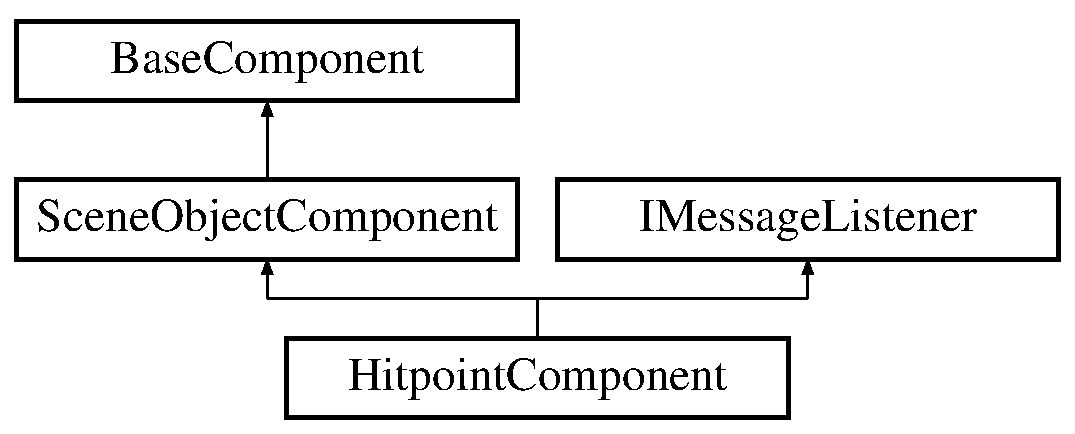
\includegraphics[height=3.000000cm]{class_hitpoint_component}
\end{center}
\end{figure}
\subsection*{Public Member Functions}
\begin{DoxyCompactItemize}
\item 
\hyperlink{class_hitpoint_component_aa2c60ad44ae7a6cb4afdc00e6ab58ae0}{Hitpoint\+Component} (\hyperlink{class_scene_object}{Scene\+Object} $\ast$parent, std\+::weak\+\_\+ptr$<$ \hyperlink{class_meta_manager}{Meta\+Manager} $>$ managers, int hitpoints)
\item 
virtual \hyperlink{class_hitpoint_component_ac860c282a3524863215e0e21a9a2c18d}{$\sim$\+Hitpoint\+Component} ()
\item 
void \hyperlink{class_hitpoint_component_ab293fcc4d167a4fa9cd27cbf1ba42018}{step} (double dt) override
\begin{DoxyCompactList}\small\item\em Step the simulation state. \end{DoxyCompactList}\item 
void \hyperlink{class_hitpoint_component_a3210abfca24e1bc9827f56533ab798af}{predraw} (\hyperlink{class_context}{Context} $\ast$context) override
\begin{DoxyCompactList}\small\item\em Called before the renderer draws the scene This allows the scene objects to do updates that require a graphics context before the graphical state is drawn. \end{DoxyCompactList}\item 
void \hyperlink{class_hitpoint_component_a86ab4e66b47a675b56c0c3eaa8ff07d9}{on\+Message} (std\+::shared\+\_\+ptr$<$ \hyperlink{class_message}{Message} $>$ msg) override
\begin{DoxyCompactList}\small\item\em Called when a message is sent to this entity. \end{DoxyCompactList}\item 
void \hyperlink{class_hitpoint_component_a7bd62f6391f68e2c8d4501372bcaf87a}{set\+Hitpoints} (int hp)
\item 
int \hyperlink{class_hitpoint_component_ae61e3e3d6c63ea20d4a54bff2e24a488}{get\+Hitpoints} () const 
\item 
void \hyperlink{class_hitpoint_component_a26d9300824f96d8dc70b0d1a6d6b74de}{deduct\+Hitpoints} (int hp)
\item 
int \hyperlink{class_hitpoint_component_a2e81eb14804005b2956f9d21caa912f0}{get\+Max\+Hitpoints} () const 
\end{DoxyCompactItemize}
\subsection*{Private Attributes}
\begin{DoxyCompactItemize}
\item 
int \hyperlink{class_hitpoint_component_a03ea97c4936474b35819c315fe2f65cb}{m\+\_\+\+Max\+Hitpoints}
\item 
int \hyperlink{class_hitpoint_component_ae113cd6a7771b75ac8a22ae1b66cfeec}{m\+\_\+\+Hitpoints}
\end{DoxyCompactItemize}
\subsection*{Additional Inherited Members}


\subsection{Detailed Description}


Definition at line 6 of file Hitpoint\+Component.\+h.



\subsection{Constructor \& Destructor Documentation}
\index{Hitpoint\+Component@{Hitpoint\+Component}!Hitpoint\+Component@{Hitpoint\+Component}}
\index{Hitpoint\+Component@{Hitpoint\+Component}!Hitpoint\+Component@{Hitpoint\+Component}}
\subsubsection[{\texorpdfstring{Hitpoint\+Component(\+Scene\+Object $\ast$parent, std\+::weak\+\_\+ptr$<$ Meta\+Manager $>$ managers, int hitpoints)}{HitpointComponent(SceneObject *parent, std::weak_ptr< MetaManager > managers, int hitpoints)}}]{\setlength{\rightskip}{0pt plus 5cm}Hitpoint\+Component\+::\+Hitpoint\+Component (
\begin{DoxyParamCaption}
\item[{{\bf Scene\+Object} $\ast$}]{parent, }
\item[{std\+::weak\+\_\+ptr$<$ {\bf Meta\+Manager} $>$}]{managers, }
\item[{int}]{hitpoints}
\end{DoxyParamCaption}
)}\hypertarget{class_hitpoint_component_aa2c60ad44ae7a6cb4afdc00e6ab58ae0}{}\label{class_hitpoint_component_aa2c60ad44ae7a6cb4afdc00e6ab58ae0}


Definition at line 8 of file Hitpoint\+Component.\+cpp.



References Message\+System\+::get\+Instance(), and Message\+System\+::subscribe().

\index{Hitpoint\+Component@{Hitpoint\+Component}!````~Hitpoint\+Component@{$\sim$\+Hitpoint\+Component}}
\index{````~Hitpoint\+Component@{$\sim$\+Hitpoint\+Component}!Hitpoint\+Component@{Hitpoint\+Component}}
\subsubsection[{\texorpdfstring{$\sim$\+Hitpoint\+Component()}{~HitpointComponent()}}]{\setlength{\rightskip}{0pt plus 5cm}Hitpoint\+Component\+::$\sim$\+Hitpoint\+Component (
\begin{DoxyParamCaption}
{}
\end{DoxyParamCaption}
)\hspace{0.3cm}{\ttfamily [virtual]}}\hypertarget{class_hitpoint_component_ac860c282a3524863215e0e21a9a2c18d}{}\label{class_hitpoint_component_ac860c282a3524863215e0e21a9a2c18d}


Definition at line 19 of file Hitpoint\+Component.\+cpp.



References Message\+System\+::get\+Instance(), and Message\+System\+::unsubscribe().



\subsection{Member Function Documentation}
\index{Hitpoint\+Component@{Hitpoint\+Component}!deduct\+Hitpoints@{deduct\+Hitpoints}}
\index{deduct\+Hitpoints@{deduct\+Hitpoints}!Hitpoint\+Component@{Hitpoint\+Component}}
\subsubsection[{\texorpdfstring{deduct\+Hitpoints(int hp)}{deductHitpoints(int hp)}}]{\setlength{\rightskip}{0pt plus 5cm}void Hitpoint\+Component\+::deduct\+Hitpoints (
\begin{DoxyParamCaption}
\item[{int}]{hp}
\end{DoxyParamCaption}
)}\hypertarget{class_hitpoint_component_a26d9300824f96d8dc70b0d1a6d6b74de}{}\label{class_hitpoint_component_a26d9300824f96d8dc70b0d1a6d6b74de}


Definition at line 52 of file Hitpoint\+Component.\+cpp.



References m\+\_\+\+Hitpoints, and m\+\_\+\+Max\+Hitpoints.



Referenced by get\+Hitpoints(), and on\+Message().

\index{Hitpoint\+Component@{Hitpoint\+Component}!get\+Hitpoints@{get\+Hitpoints}}
\index{get\+Hitpoints@{get\+Hitpoints}!Hitpoint\+Component@{Hitpoint\+Component}}
\subsubsection[{\texorpdfstring{get\+Hitpoints() const }{getHitpoints() const }}]{\setlength{\rightskip}{0pt plus 5cm}int Hitpoint\+Component\+::get\+Hitpoints (
\begin{DoxyParamCaption}
{}
\end{DoxyParamCaption}
) const\hspace{0.3cm}{\ttfamily [inline]}}\hypertarget{class_hitpoint_component_ae61e3e3d6c63ea20d4a54bff2e24a488}{}\label{class_hitpoint_component_ae61e3e3d6c63ea20d4a54bff2e24a488}


Definition at line 26 of file Hitpoint\+Component.\+h.



References deduct\+Hitpoints(), and m\+\_\+\+Hitpoints.

\index{Hitpoint\+Component@{Hitpoint\+Component}!get\+Max\+Hitpoints@{get\+Max\+Hitpoints}}
\index{get\+Max\+Hitpoints@{get\+Max\+Hitpoints}!Hitpoint\+Component@{Hitpoint\+Component}}
\subsubsection[{\texorpdfstring{get\+Max\+Hitpoints() const }{getMaxHitpoints() const }}]{\setlength{\rightskip}{0pt plus 5cm}int Hitpoint\+Component\+::get\+Max\+Hitpoints (
\begin{DoxyParamCaption}
{}
\end{DoxyParamCaption}
) const\hspace{0.3cm}{\ttfamily [inline]}}\hypertarget{class_hitpoint_component_a2e81eb14804005b2956f9d21caa912f0}{}\label{class_hitpoint_component_a2e81eb14804005b2956f9d21caa912f0}


Definition at line 30 of file Hitpoint\+Component.\+h.



References m\+\_\+\+Max\+Hitpoints.

\index{Hitpoint\+Component@{Hitpoint\+Component}!on\+Message@{on\+Message}}
\index{on\+Message@{on\+Message}!Hitpoint\+Component@{Hitpoint\+Component}}
\subsubsection[{\texorpdfstring{on\+Message(std\+::shared\+\_\+ptr$<$ Message $>$ msg) override}{onMessage(std::shared_ptr< Message > msg) override}}]{\setlength{\rightskip}{0pt plus 5cm}void Hitpoint\+Component\+::on\+Message (
\begin{DoxyParamCaption}
\item[{std\+::shared\+\_\+ptr$<$ {\bf Message} $>$}]{msg}
\end{DoxyParamCaption}
)\hspace{0.3cm}{\ttfamily [override]}, {\ttfamily [virtual]}}\hypertarget{class_hitpoint_component_a86ab4e66b47a675b56c0c3eaa8ff07d9}{}\label{class_hitpoint_component_a86ab4e66b47a675b56c0c3eaa8ff07d9}


Called when a message is sent to this entity. 


\begin{DoxyParams}{Parameters}
{\em msg} & Smart pointer to the received message object \\
\hline
\end{DoxyParams}


Implements \hyperlink{class_i_message_listener_aac85f64eeb587944c59e07f5457b1b82}{I\+Message\+Listener}.



Definition at line 25 of file Hitpoint\+Component.\+cpp.



References Message\+System\+::broadcast(), deduct\+Hitpoints(), Message\+System\+::get\+Instance(), Scene\+Object\+Component\+::get\+Parent(), and m\+\_\+\+Hitpoints.



Referenced by predraw().

\index{Hitpoint\+Component@{Hitpoint\+Component}!predraw@{predraw}}
\index{predraw@{predraw}!Hitpoint\+Component@{Hitpoint\+Component}}
\subsubsection[{\texorpdfstring{predraw(\+Context $\ast$context) override}{predraw(Context *context) override}}]{\setlength{\rightskip}{0pt plus 5cm}void Hitpoint\+Component\+::predraw (
\begin{DoxyParamCaption}
\item[{{\bf Context} $\ast$}]{context}
\end{DoxyParamCaption}
)\hspace{0.3cm}{\ttfamily [inline]}, {\ttfamily [override]}, {\ttfamily [virtual]}}\hypertarget{class_hitpoint_component_a3210abfca24e1bc9827f56533ab798af}{}\label{class_hitpoint_component_a3210abfca24e1bc9827f56533ab798af}


Called before the renderer draws the scene This allows the scene objects to do updates that require a graphics context before the graphical state is drawn. 


\begin{DoxyParams}{Parameters}
{\em context} & Graphics context \\
\hline
\end{DoxyParams}


Implements \hyperlink{class_scene_object_component_a7110e37ad23a708c2bf9828c7fd7df2f}{Scene\+Object\+Component}.



Definition at line 20 of file Hitpoint\+Component.\+h.



References on\+Message(), and set\+Hitpoints().

\index{Hitpoint\+Component@{Hitpoint\+Component}!set\+Hitpoints@{set\+Hitpoints}}
\index{set\+Hitpoints@{set\+Hitpoints}!Hitpoint\+Component@{Hitpoint\+Component}}
\subsubsection[{\texorpdfstring{set\+Hitpoints(int hp)}{setHitpoints(int hp)}}]{\setlength{\rightskip}{0pt plus 5cm}void Hitpoint\+Component\+::set\+Hitpoints (
\begin{DoxyParamCaption}
\item[{int}]{hp}
\end{DoxyParamCaption}
)}\hypertarget{class_hitpoint_component_a7bd62f6391f68e2c8d4501372bcaf87a}{}\label{class_hitpoint_component_a7bd62f6391f68e2c8d4501372bcaf87a}


Definition at line 45 of file Hitpoint\+Component.\+cpp.



References m\+\_\+\+Hitpoints, and m\+\_\+\+Max\+Hitpoints.



Referenced by predraw().

\index{Hitpoint\+Component@{Hitpoint\+Component}!step@{step}}
\index{step@{step}!Hitpoint\+Component@{Hitpoint\+Component}}
\subsubsection[{\texorpdfstring{step(double dt) override}{step(double dt) override}}]{\setlength{\rightskip}{0pt plus 5cm}void Hitpoint\+Component\+::step (
\begin{DoxyParamCaption}
\item[{double}]{dt}
\end{DoxyParamCaption}
)\hspace{0.3cm}{\ttfamily [inline]}, {\ttfamily [override]}, {\ttfamily [virtual]}}\hypertarget{class_hitpoint_component_ab293fcc4d167a4fa9cd27cbf1ba42018}{}\label{class_hitpoint_component_ab293fcc4d167a4fa9cd27cbf1ba42018}


Step the simulation state. 


\begin{DoxyParams}{Parameters}
{\em dt} & Delta-\/time since last step call in seconds \\
\hline
\end{DoxyParams}


Implements \hyperlink{class_scene_object_component_a99ebed011a6547be4d31a09927e3b810}{Scene\+Object\+Component}.



Definition at line 18 of file Hitpoint\+Component.\+h.



\subsection{Member Data Documentation}
\index{Hitpoint\+Component@{Hitpoint\+Component}!m\+\_\+\+Hitpoints@{m\+\_\+\+Hitpoints}}
\index{m\+\_\+\+Hitpoints@{m\+\_\+\+Hitpoints}!Hitpoint\+Component@{Hitpoint\+Component}}
\subsubsection[{\texorpdfstring{m\+\_\+\+Hitpoints}{m_Hitpoints}}]{\setlength{\rightskip}{0pt plus 5cm}int Hitpoint\+Component\+::m\+\_\+\+Hitpoints\hspace{0.3cm}{\ttfamily [private]}}\hypertarget{class_hitpoint_component_ae113cd6a7771b75ac8a22ae1b66cfeec}{}\label{class_hitpoint_component_ae113cd6a7771b75ac8a22ae1b66cfeec}


Definition at line 34 of file Hitpoint\+Component.\+h.



Referenced by deduct\+Hitpoints(), get\+Hitpoints(), on\+Message(), and set\+Hitpoints().

\index{Hitpoint\+Component@{Hitpoint\+Component}!m\+\_\+\+Max\+Hitpoints@{m\+\_\+\+Max\+Hitpoints}}
\index{m\+\_\+\+Max\+Hitpoints@{m\+\_\+\+Max\+Hitpoints}!Hitpoint\+Component@{Hitpoint\+Component}}
\subsubsection[{\texorpdfstring{m\+\_\+\+Max\+Hitpoints}{m_MaxHitpoints}}]{\setlength{\rightskip}{0pt plus 5cm}int Hitpoint\+Component\+::m\+\_\+\+Max\+Hitpoints\hspace{0.3cm}{\ttfamily [private]}}\hypertarget{class_hitpoint_component_a03ea97c4936474b35819c315fe2f65cb}{}\label{class_hitpoint_component_a03ea97c4936474b35819c315fe2f65cb}


Definition at line 33 of file Hitpoint\+Component.\+h.



Referenced by deduct\+Hitpoints(), get\+Max\+Hitpoints(), and set\+Hitpoints().



The documentation for this class was generated from the following files\+:\begin{DoxyCompactItemize}
\item 
Lunar\+Drift/engine/components/\hyperlink{_hitpoint_component_8h}{Hitpoint\+Component.\+h}\item 
Lunar\+Drift/engine/components/\hyperlink{_hitpoint_component_8cpp}{Hitpoint\+Component.\+cpp}\end{DoxyCompactItemize}

\hypertarget{class_i_message_listener}{}\section{I\+Message\+Listener Class Reference}
\label{class_i_message_listener}\index{I\+Message\+Listener@{I\+Message\+Listener}}


Interface for handling messages sent from other entities.  




{\ttfamily \#include $<$I\+Message\+Listener.\+h$>$}

Inheritance diagram for I\+Message\+Listener\+:\begin{figure}[H]
\begin{center}
\leavevmode
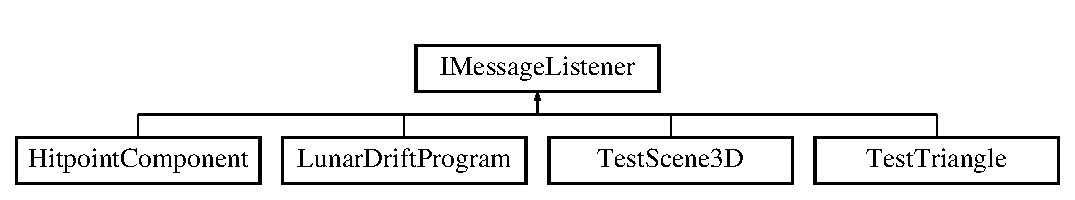
\includegraphics[height=2.000000cm]{class_i_message_listener}
\end{center}
\end{figure}
\subsection*{Public Member Functions}
\begin{DoxyCompactItemize}
\item 
virtual \hyperlink{class_i_message_listener_af09a1fa8b00d182a92f357ad89a024a5}{$\sim$\+I\+Message\+Listener} ()
\item 
virtual void \hyperlink{class_i_message_listener_aac85f64eeb587944c59e07f5457b1b82}{on\+Message} (std\+::shared\+\_\+ptr$<$ \hyperlink{class_message}{Message} $>$ msg)=0
\begin{DoxyCompactList}\small\item\em Called when a message is sent to this entity. \end{DoxyCompactList}\end{DoxyCompactItemize}


\subsection{Detailed Description}
Interface for handling messages sent from other entities. 

Messages are packets of data sent between entities in the program. Events operate in a broadcast fashion, messages operate in a unicast fashion with a sender and a receiver at the point of handling.

\begin{DoxyAuthor}{Author}
Hayley Hatton 
\end{DoxyAuthor}
\begin{DoxyDate}{Date}
10/03/2016 
\end{DoxyDate}
\begin{DoxySeeAlso}{See also}
\hyperlink{class_message}{Message} 

\hyperlink{class_message_system}{Message\+System} 
\end{DoxySeeAlso}


Definition at line 18 of file I\+Message\+Listener.\+h.



\subsection{Constructor \& Destructor Documentation}
\index{I\+Message\+Listener@{I\+Message\+Listener}!````~I\+Message\+Listener@{$\sim$\+I\+Message\+Listener}}
\index{````~I\+Message\+Listener@{$\sim$\+I\+Message\+Listener}!I\+Message\+Listener@{I\+Message\+Listener}}
\subsubsection[{\texorpdfstring{$\sim$\+I\+Message\+Listener()}{~IMessageListener()}}]{\setlength{\rightskip}{0pt plus 5cm}virtual I\+Message\+Listener\+::$\sim$\+I\+Message\+Listener (
\begin{DoxyParamCaption}
{}
\end{DoxyParamCaption}
)\hspace{0.3cm}{\ttfamily [inline]}, {\ttfamily [virtual]}}\hypertarget{class_i_message_listener_af09a1fa8b00d182a92f357ad89a024a5}{}\label{class_i_message_listener_af09a1fa8b00d182a92f357ad89a024a5}


Definition at line 21 of file I\+Message\+Listener.\+h.



References on\+Message().



\subsection{Member Function Documentation}
\index{I\+Message\+Listener@{I\+Message\+Listener}!on\+Message@{on\+Message}}
\index{on\+Message@{on\+Message}!I\+Message\+Listener@{I\+Message\+Listener}}
\subsubsection[{\texorpdfstring{on\+Message(std\+::shared\+\_\+ptr$<$ Message $>$ msg)=0}{onMessage(std::shared_ptr< Message > msg)=0}}]{\setlength{\rightskip}{0pt plus 5cm}virtual void I\+Message\+Listener\+::on\+Message (
\begin{DoxyParamCaption}
\item[{std\+::shared\+\_\+ptr$<$ {\bf Message} $>$}]{msg}
\end{DoxyParamCaption}
)\hspace{0.3cm}{\ttfamily [pure virtual]}}\hypertarget{class_i_message_listener_aac85f64eeb587944c59e07f5457b1b82}{}\label{class_i_message_listener_aac85f64eeb587944c59e07f5457b1b82}


Called when a message is sent to this entity. 


\begin{DoxyParams}{Parameters}
{\em msg} & Smart pointer to the received message object \\
\hline
\end{DoxyParams}


Implemented in \hyperlink{class_test_scene3_d_aa5c6527ffc929e51eb3303431bfc6f7d}{Test\+Scene3D}, \hyperlink{class_lunar_drift_program_a6586725d0267426dae45c7c5772cffc2}{Lunar\+Drift\+Program}, \hyperlink{class_test_triangle_ac5165e9e0ecdc4b232752b49c1ecbec0}{Test\+Triangle}, and \hyperlink{class_hitpoint_component_a86ab4e66b47a675b56c0c3eaa8ff07d9}{Hitpoint\+Component}.



Referenced by Life\+Time\+Component\+::step(), and $\sim$\+I\+Message\+Listener().



The documentation for this class was generated from the following file\+:\begin{DoxyCompactItemize}
\item 
Lunar\+Drift/engine/comms/\hyperlink{_i_message_listener_8h}{I\+Message\+Listener.\+h}\end{DoxyCompactItemize}

\hypertarget{class_index_buffer_object}{}\section{Index\+Buffer\+Object Class Reference}
\label{class_index_buffer_object}\index{Index\+Buffer\+Object@{Index\+Buffer\+Object}}


Buffer manager for model indices.  




{\ttfamily \#include $<$Index\+Buffer\+Object.\+h$>$}

\subsection*{Public Member Functions}
\begin{DoxyCompactItemize}
\item 
\hyperlink{class_index_buffer_object_af68b0d097152e2956479d931d553057f}{Index\+Buffer\+Object} (\hyperlink{class_context}{Context} $\ast$context, const std\+::vector$<$ unsigned short $>$ \&indices)
\begin{DoxyCompactList}\small\item\em Default constructor. Creates the I\+BO buffer on the G\+PU. \end{DoxyCompactList}\item 
virtual \hyperlink{class_index_buffer_object_ab90647bffb075f60071e404260881731}{$\sim$\+Index\+Buffer\+Object} ()
\begin{DoxyCompactList}\small\item\em Default destructor. Destroys the I\+BO buffer. \end{DoxyCompactList}\item 
void \hyperlink{class_index_buffer_object_aff2a0368134dec8cad54605d5435ba25}{bind} (\hyperlink{class_context}{Context} $\ast$context)
\begin{DoxyCompactList}\small\item\em Binds the I\+BO to the Open\+GL pipeline. \end{DoxyCompactList}\item 
unsigned int \hyperlink{class_index_buffer_object_a1d23270c5c1e3a39c48a98cb13abe80f}{size} () const 
\begin{DoxyCompactList}\small\item\em Access the amount of indices in the I\+BO. \end{DoxyCompactList}\item 
G\+Lenum \hyperlink{class_index_buffer_object_aa819995c955a645ca8db56fbdf3fcbbe}{get\+Open\+G\+L\+Class} () const 
\begin{DoxyCompactList}\small\item\em Access the Open\+GL integer class of the indices stored in the I\+BO. \end{DoxyCompactList}\end{DoxyCompactItemize}
\subsection*{Private Attributes}
\begin{DoxyCompactItemize}
\item 
std\+::vector$<$ unsigned short $>$ \hyperlink{class_index_buffer_object_a990bafed8ff20200858ce93a833019af}{m\+\_\+\+Indices}
\begin{DoxyCompactList}\small\item\em Index buffer. \end{DoxyCompactList}\item 
G\+Luint \hyperlink{class_index_buffer_object_a861d3d51556c2e639d626a74d9ff71c6}{m\+\_\+\+I\+BO}
\begin{DoxyCompactList}\small\item\em Open\+G\+L-\/provided I\+BO handle. \end{DoxyCompactList}\end{DoxyCompactItemize}


\subsection{Detailed Description}
Buffer manager for model indices. 

Index buffer objects (or I\+B\+Os) in Open\+GL describe the order in which vertices are drawn, which allow models to be drawn without repeating vertices.

\begin{DoxyPrecond}{Precondition}
A valid Open\+GL context must be present to the program 
\end{DoxyPrecond}
\begin{DoxyAuthor}{Author}
Hayley Hatton 
\end{DoxyAuthor}
\begin{DoxyDate}{Date}
20/02/2016 
\end{DoxyDate}
\begin{DoxySeeAlso}{See also}
\hyperlink{class_vertex_array_object}{Vertex\+Array\+Object} 
\end{DoxySeeAlso}
\begin{DoxyRefDesc}{Todo}
\item[\hyperlink{todo__todo000006}{Todo}](Hayley\#6\#02/22/16)\+: Handling of dynamic buffers and syncronicity between C\+PU and G\+PU \end{DoxyRefDesc}


Definition at line 18 of file Index\+Buffer\+Object.\+h.



\subsection{Constructor \& Destructor Documentation}
\index{Index\+Buffer\+Object@{Index\+Buffer\+Object}!Index\+Buffer\+Object@{Index\+Buffer\+Object}}
\index{Index\+Buffer\+Object@{Index\+Buffer\+Object}!Index\+Buffer\+Object@{Index\+Buffer\+Object}}
\subsubsection[{\texorpdfstring{Index\+Buffer\+Object(\+Context $\ast$context, const std\+::vector$<$ unsigned short $>$ \&indices)}{IndexBufferObject(Context *context, const std::vector< unsigned short > &indices)}}]{\setlength{\rightskip}{0pt plus 5cm}Index\+Buffer\+Object\+::\+Index\+Buffer\+Object (
\begin{DoxyParamCaption}
\item[{{\bf Context} $\ast$}]{context, }
\item[{const std\+::vector$<$ unsigned short $>$ \&}]{indices}
\end{DoxyParamCaption}
)}\hypertarget{class_index_buffer_object_af68b0d097152e2956479d931d553057f}{}\label{class_index_buffer_object_af68b0d097152e2956479d931d553057f}


Default constructor. Creates the I\+BO buffer on the G\+PU. 


\begin{DoxyParams}{Parameters}
{\em context} & Graphics context \\
\hline
{\em indices} & Initial index buffer state \\
\hline
\end{DoxyParams}


Definition at line 5 of file Index\+Buffer\+Object.\+cpp.



References bind(), and m\+\_\+\+I\+BO.

\index{Index\+Buffer\+Object@{Index\+Buffer\+Object}!````~Index\+Buffer\+Object@{$\sim$\+Index\+Buffer\+Object}}
\index{````~Index\+Buffer\+Object@{$\sim$\+Index\+Buffer\+Object}!Index\+Buffer\+Object@{Index\+Buffer\+Object}}
\subsubsection[{\texorpdfstring{$\sim$\+Index\+Buffer\+Object()}{~IndexBufferObject()}}]{\setlength{\rightskip}{0pt plus 5cm}Index\+Buffer\+Object\+::$\sim$\+Index\+Buffer\+Object (
\begin{DoxyParamCaption}
{}
\end{DoxyParamCaption}
)\hspace{0.3cm}{\ttfamily [virtual]}}\hypertarget{class_index_buffer_object_ab90647bffb075f60071e404260881731}{}\label{class_index_buffer_object_ab90647bffb075f60071e404260881731}


Default destructor. Destroys the I\+BO buffer. 



Definition at line 31 of file Index\+Buffer\+Object.\+cpp.



References m\+\_\+\+I\+BO.



\subsection{Member Function Documentation}
\index{Index\+Buffer\+Object@{Index\+Buffer\+Object}!bind@{bind}}
\index{bind@{bind}!Index\+Buffer\+Object@{Index\+Buffer\+Object}}
\subsubsection[{\texorpdfstring{bind(\+Context $\ast$context)}{bind(Context *context)}}]{\setlength{\rightskip}{0pt plus 5cm}void Index\+Buffer\+Object\+::bind (
\begin{DoxyParamCaption}
\item[{{\bf Context} $\ast$}]{context}
\end{DoxyParamCaption}
)}\hypertarget{class_index_buffer_object_aff2a0368134dec8cad54605d5435ba25}{}\label{class_index_buffer_object_aff2a0368134dec8cad54605d5435ba25}


Binds the I\+BO to the Open\+GL pipeline. 


\begin{DoxyParams}{Parameters}
{\em context} & Graphics context \\
\hline
\end{DoxyParams}


Definition at line 37 of file Index\+Buffer\+Object.\+cpp.



References m\+\_\+\+I\+BO.



Referenced by Index\+Buffer\+Object().

\index{Index\+Buffer\+Object@{Index\+Buffer\+Object}!get\+Open\+G\+L\+Class@{get\+Open\+G\+L\+Class}}
\index{get\+Open\+G\+L\+Class@{get\+Open\+G\+L\+Class}!Index\+Buffer\+Object@{Index\+Buffer\+Object}}
\subsubsection[{\texorpdfstring{get\+Open\+G\+L\+Class() const }{getOpenGLClass() const }}]{\setlength{\rightskip}{0pt plus 5cm}G\+Lenum Index\+Buffer\+Object\+::get\+Open\+G\+L\+Class (
\begin{DoxyParamCaption}
{}
\end{DoxyParamCaption}
) const\hspace{0.3cm}{\ttfamily [inline]}}\hypertarget{class_index_buffer_object_aa819995c955a645ca8db56fbdf3fcbbe}{}\label{class_index_buffer_object_aa819995c955a645ca8db56fbdf3fcbbe}


Access the Open\+GL integer class of the indices stored in the I\+BO. 

\begin{DoxyReturn}{Returns}
Open\+GL enumerator describing the integer size 
\end{DoxyReturn}


Definition at line 50 of file Index\+Buffer\+Object.\+h.

\index{Index\+Buffer\+Object@{Index\+Buffer\+Object}!size@{size}}
\index{size@{size}!Index\+Buffer\+Object@{Index\+Buffer\+Object}}
\subsubsection[{\texorpdfstring{size() const }{size() const }}]{\setlength{\rightskip}{0pt plus 5cm}unsigned int Index\+Buffer\+Object\+::size (
\begin{DoxyParamCaption}
{}
\end{DoxyParamCaption}
) const\hspace{0.3cm}{\ttfamily [inline]}}\hypertarget{class_index_buffer_object_a1d23270c5c1e3a39c48a98cb13abe80f}{}\label{class_index_buffer_object_a1d23270c5c1e3a39c48a98cb13abe80f}


Access the amount of indices in the I\+BO. 

\begin{DoxyReturn}{Returns}
Number of elements in the I\+BO 
\end{DoxyReturn}


Definition at line 44 of file Index\+Buffer\+Object.\+h.



References m\+\_\+\+Indices.



\subsection{Member Data Documentation}
\index{Index\+Buffer\+Object@{Index\+Buffer\+Object}!m\+\_\+\+I\+BO@{m\+\_\+\+I\+BO}}
\index{m\+\_\+\+I\+BO@{m\+\_\+\+I\+BO}!Index\+Buffer\+Object@{Index\+Buffer\+Object}}
\subsubsection[{\texorpdfstring{m\+\_\+\+I\+BO}{m_IBO}}]{\setlength{\rightskip}{0pt plus 5cm}G\+Luint Index\+Buffer\+Object\+::m\+\_\+\+I\+BO\hspace{0.3cm}{\ttfamily [private]}}\hypertarget{class_index_buffer_object_a861d3d51556c2e639d626a74d9ff71c6}{}\label{class_index_buffer_object_a861d3d51556c2e639d626a74d9ff71c6}


Open\+G\+L-\/provided I\+BO handle. 



Definition at line 54 of file Index\+Buffer\+Object.\+h.



Referenced by bind(), Index\+Buffer\+Object(), and $\sim$\+Index\+Buffer\+Object().

\index{Index\+Buffer\+Object@{Index\+Buffer\+Object}!m\+\_\+\+Indices@{m\+\_\+\+Indices}}
\index{m\+\_\+\+Indices@{m\+\_\+\+Indices}!Index\+Buffer\+Object@{Index\+Buffer\+Object}}
\subsubsection[{\texorpdfstring{m\+\_\+\+Indices}{m_Indices}}]{\setlength{\rightskip}{0pt plus 5cm}std\+::vector$<$unsigned short$>$ Index\+Buffer\+Object\+::m\+\_\+\+Indices\hspace{0.3cm}{\ttfamily [private]}}\hypertarget{class_index_buffer_object_a990bafed8ff20200858ce93a833019af}{}\label{class_index_buffer_object_a990bafed8ff20200858ce93a833019af}


Index buffer. 



Definition at line 53 of file Index\+Buffer\+Object.\+h.



Referenced by size().



The documentation for this class was generated from the following files\+:\begin{DoxyCompactItemize}
\item 
Lunar\+Drift/engine/graphics/buffers/\hyperlink{_index_buffer_object_8h}{Index\+Buffer\+Object.\+h}\item 
Lunar\+Drift/engine/graphics/buffers/\hyperlink{_index_buffer_object_8cpp}{Index\+Buffer\+Object.\+cpp}\end{DoxyCompactItemize}

\hypertarget{class_input_event}{}\section{Input\+Event Class Reference}
\label{class_input_event}\index{Input\+Event@{Input\+Event}}


{\ttfamily \#include $<$Input\+Event.\+h$>$}

Inheritance diagram for Input\+Event\+:\begin{figure}[H]
\begin{center}
\leavevmode
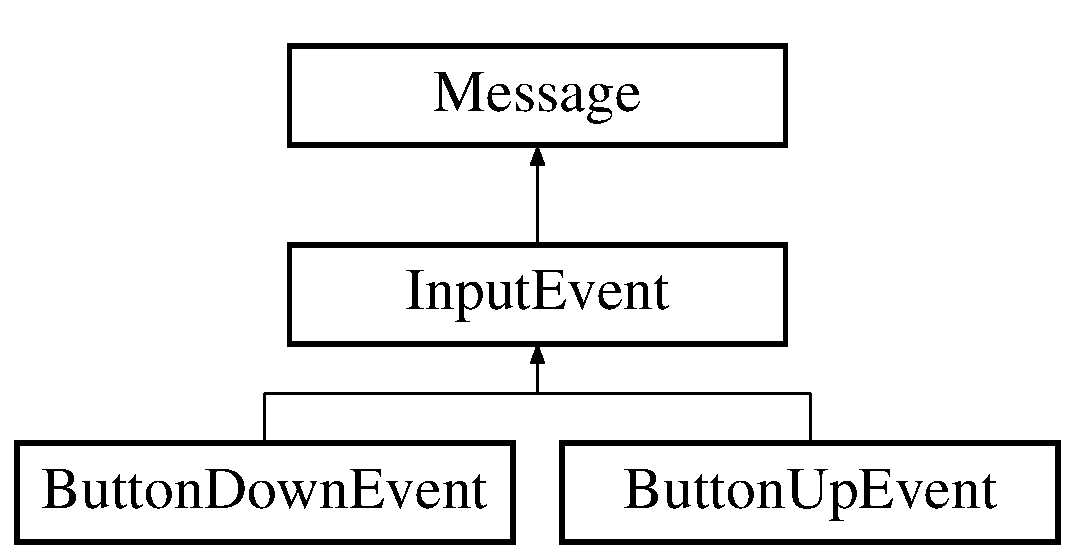
\includegraphics[height=3.000000cm]{class_input_event}
\end{center}
\end{figure}
\subsection*{Public Member Functions}
\begin{DoxyCompactItemize}
\item 
\hyperlink{class_input_event_a64b326dc5bc3ce1822155dea69d0a8a3}{Input\+Event} (const std\+::string \&type)
\item 
virtual \hyperlink{class_input_event_a2ac246c18ad2647d8cd2f62f7a60bc39}{$\sim$\+Input\+Event} ()
\end{DoxyCompactItemize}


\subsection{Detailed Description}


Definition at line 6 of file Input\+Event.\+h.



\subsection{Constructor \& Destructor Documentation}
\index{Input\+Event@{Input\+Event}!Input\+Event@{Input\+Event}}
\index{Input\+Event@{Input\+Event}!Input\+Event@{Input\+Event}}
\subsubsection[{\texorpdfstring{Input\+Event(const std\+::string \&type)}{InputEvent(const std::string &type)}}]{\setlength{\rightskip}{0pt plus 5cm}Input\+Event\+::\+Input\+Event (
\begin{DoxyParamCaption}
\item[{const std\+::string \&}]{type}
\end{DoxyParamCaption}
)}\hypertarget{class_input_event_a64b326dc5bc3ce1822155dea69d0a8a3}{}\label{class_input_event_a64b326dc5bc3ce1822155dea69d0a8a3}
Default constructor 

Definition at line 3 of file Input\+Event.\+cpp.

\index{Input\+Event@{Input\+Event}!````~Input\+Event@{$\sim$\+Input\+Event}}
\index{````~Input\+Event@{$\sim$\+Input\+Event}!Input\+Event@{Input\+Event}}
\subsubsection[{\texorpdfstring{$\sim$\+Input\+Event()}{~InputEvent()}}]{\setlength{\rightskip}{0pt plus 5cm}Input\+Event\+::$\sim$\+Input\+Event (
\begin{DoxyParamCaption}
{}
\end{DoxyParamCaption}
)\hspace{0.3cm}{\ttfamily [virtual]}}\hypertarget{class_input_event_a2ac246c18ad2647d8cd2f62f7a60bc39}{}\label{class_input_event_a2ac246c18ad2647d8cd2f62f7a60bc39}
Default destructor 

Definition at line 8 of file Input\+Event.\+cpp.



The documentation for this class was generated from the following files\+:\begin{DoxyCompactItemize}
\item 
Lunar\+Drift/engine/comms/predefined/\hyperlink{_input_event_8h}{Input\+Event.\+h}\item 
Lunar\+Drift/engine/comms/predefined/\hyperlink{_input_event_8cpp}{Input\+Event.\+cpp}\end{DoxyCompactItemize}

\hypertarget{class_input_map}{}\section{Input\+Map Class Reference}
\label{class_input_map}\index{Input\+Map@{Input\+Map}}


{\ttfamily \#include $<$Input\+Map.\+h$>$}

\subsection*{Public Member Functions}
\begin{DoxyCompactItemize}
\item 
\hyperlink{class_keyboard}{Keyboard} $\ast$ \hyperlink{class_input_map_abce4326eae5855278d5820f8c8be6ddf}{get\+Keyboard} ()
\end{DoxyCompactItemize}
\subsection*{Static Public Member Functions}
\begin{DoxyCompactItemize}
\item 
static \hyperlink{class_input_map}{Input\+Map} \& \hyperlink{class_input_map_ae2eeb0a6d7d6274d8d50f6557a42cbdd}{get\+Instance} ()
\end{DoxyCompactItemize}
\subsection*{Private Member Functions}
\begin{DoxyCompactItemize}
\item 
\hyperlink{class_input_map_aa79c436a267244b2151a564a56ac8b38}{Input\+Map} ()
\item 
\hyperlink{class_input_map_ae7be3f13a088f8c4bc03504a4413317f}{Input\+Map} (\hyperlink{class_input_map}{Input\+Map} const \&)=delete
\item 
void \hyperlink{class_input_map_adfecb2628e99c4a50b4ebf50bf5494fc}{operator=} (\hyperlink{class_input_map}{Input\+Map} const \&)=delete
\end{DoxyCompactItemize}
\subsection*{Private Attributes}
\begin{DoxyCompactItemize}
\item 
\hyperlink{class_keyboard}{Keyboard} \hyperlink{class_input_map_ae1f1c18ccacc60010acc66c2b8d5fe53}{m\+\_\+\+Keyboard}
\end{DoxyCompactItemize}


\subsection{Detailed Description}


Definition at line 5 of file Input\+Map.\+h.



\subsection{Constructor \& Destructor Documentation}
\index{Input\+Map@{Input\+Map}!Input\+Map@{Input\+Map}}
\index{Input\+Map@{Input\+Map}!Input\+Map@{Input\+Map}}
\subsubsection[{\texorpdfstring{Input\+Map()}{InputMap()}}]{\setlength{\rightskip}{0pt plus 5cm}Input\+Map\+::\+Input\+Map (
\begin{DoxyParamCaption}
{}
\end{DoxyParamCaption}
)\hspace{0.3cm}{\ttfamily [inline]}, {\ttfamily [private]}}\hypertarget{class_input_map_aa79c436a267244b2151a564a56ac8b38}{}\label{class_input_map_aa79c436a267244b2151a564a56ac8b38}


Definition at line 24 of file Input\+Map.\+h.



References operator=().

\index{Input\+Map@{Input\+Map}!Input\+Map@{Input\+Map}}
\index{Input\+Map@{Input\+Map}!Input\+Map@{Input\+Map}}
\subsubsection[{\texorpdfstring{Input\+Map(\+Input\+Map const \&)=delete}{InputMap(InputMap const &)=delete}}]{\setlength{\rightskip}{0pt plus 5cm}Input\+Map\+::\+Input\+Map (
\begin{DoxyParamCaption}
\item[{{\bf Input\+Map} const \&}]{}
\end{DoxyParamCaption}
)\hspace{0.3cm}{\ttfamily [private]}, {\ttfamily [delete]}}\hypertarget{class_input_map_ae7be3f13a088f8c4bc03504a4413317f}{}\label{class_input_map_ae7be3f13a088f8c4bc03504a4413317f}


\subsection{Member Function Documentation}
\index{Input\+Map@{Input\+Map}!get\+Instance@{get\+Instance}}
\index{get\+Instance@{get\+Instance}!Input\+Map@{Input\+Map}}
\subsubsection[{\texorpdfstring{get\+Instance()}{getInstance()}}]{\setlength{\rightskip}{0pt plus 5cm}static {\bf Input\+Map}\& Input\+Map\+::get\+Instance (
\begin{DoxyParamCaption}
{}
\end{DoxyParamCaption}
)\hspace{0.3cm}{\ttfamily [inline]}, {\ttfamily [static]}}\hypertarget{class_input_map_ae2eeb0a6d7d6274d8d50f6557a42cbdd}{}\label{class_input_map_ae2eeb0a6d7d6274d8d50f6557a42cbdd}


Definition at line 8 of file Input\+Map.\+h.



Referenced by Window\+P\+C\+::handle\+Win32\+Event\+Queue(), Lunar\+Drift\+Program\+::\+Lunar\+Drift\+Program(), and Test\+Scene3\+D\+::step().

\index{Input\+Map@{Input\+Map}!get\+Keyboard@{get\+Keyboard}}
\index{get\+Keyboard@{get\+Keyboard}!Input\+Map@{Input\+Map}}
\subsubsection[{\texorpdfstring{get\+Keyboard()}{getKeyboard()}}]{\setlength{\rightskip}{0pt plus 5cm}{\bf Keyboard}$\ast$ Input\+Map\+::get\+Keyboard (
\begin{DoxyParamCaption}
{}
\end{DoxyParamCaption}
)\hspace{0.3cm}{\ttfamily [inline]}}\hypertarget{class_input_map_abce4326eae5855278d5820f8c8be6ddf}{}\label{class_input_map_abce4326eae5855278d5820f8c8be6ddf}


Definition at line 14 of file Input\+Map.\+h.



References m\+\_\+\+Keyboard.



Referenced by Window\+P\+C\+::handle\+Win32\+Event\+Queue(), Lunar\+Drift\+Program\+::\+Lunar\+Drift\+Program(), and Test\+Scene3\+D\+::step().

\index{Input\+Map@{Input\+Map}!operator=@{operator=}}
\index{operator=@{operator=}!Input\+Map@{Input\+Map}}
\subsubsection[{\texorpdfstring{operator=(\+Input\+Map const \&)=delete}{operator=(InputMap const &)=delete}}]{\setlength{\rightskip}{0pt plus 5cm}void Input\+Map\+::operator= (
\begin{DoxyParamCaption}
\item[{{\bf Input\+Map} const \&}]{}
\end{DoxyParamCaption}
)\hspace{0.3cm}{\ttfamily [private]}, {\ttfamily [delete]}}\hypertarget{class_input_map_adfecb2628e99c4a50b4ebf50bf5494fc}{}\label{class_input_map_adfecb2628e99c4a50b4ebf50bf5494fc}


Referenced by Input\+Map().



\subsection{Member Data Documentation}
\index{Input\+Map@{Input\+Map}!m\+\_\+\+Keyboard@{m\+\_\+\+Keyboard}}
\index{m\+\_\+\+Keyboard@{m\+\_\+\+Keyboard}!Input\+Map@{Input\+Map}}
\subsubsection[{\texorpdfstring{m\+\_\+\+Keyboard}{m_Keyboard}}]{\setlength{\rightskip}{0pt plus 5cm}{\bf Keyboard} Input\+Map\+::m\+\_\+\+Keyboard\hspace{0.3cm}{\ttfamily [private]}}\hypertarget{class_input_map_ae1f1c18ccacc60010acc66c2b8d5fe53}{}\label{class_input_map_ae1f1c18ccacc60010acc66c2b8d5fe53}


Definition at line 20 of file Input\+Map.\+h.



Referenced by get\+Keyboard().



The documentation for this class was generated from the following file\+:\begin{DoxyCompactItemize}
\item 
Lunar\+Drift/engine/input/\hyperlink{_input_map_8h}{Input\+Map.\+h}\end{DoxyCompactItemize}

\hypertarget{class_joystick}{}\section{Joystick Class Reference}
\label{class_joystick}\index{Joystick@{Joystick}}


{\ttfamily \#include $<$Joystick.\+h$>$}

\subsection*{Public Member Functions}
\begin{DoxyCompactItemize}
\item 
\hyperlink{class_joystick_a158b1f77b78717efbf1b8fac43b1fcef}{Joystick} ()
\item 
virtual \hyperlink{class_joystick_a23429c0470e1a32b8de61e1ad7c251c1}{$\sim$\+Joystick} ()
\end{DoxyCompactItemize}
\subsection*{Private Attributes}
\begin{DoxyCompactItemize}
\item 
glm\+::vec2 \hyperlink{class_joystick_abfad27b592642f59b66060dec430f91c}{m\+\_\+\+Position}
\end{DoxyCompactItemize}


\subsection{Detailed Description}


Definition at line 5 of file Joystick.\+h.



\subsection{Constructor \& Destructor Documentation}
\index{Joystick@{Joystick}!Joystick@{Joystick}}
\index{Joystick@{Joystick}!Joystick@{Joystick}}
\subsubsection[{\texorpdfstring{Joystick()}{Joystick()}}]{\setlength{\rightskip}{0pt plus 5cm}Joystick\+::\+Joystick (
\begin{DoxyParamCaption}
{}
\end{DoxyParamCaption}
)}\hypertarget{class_joystick_a158b1f77b78717efbf1b8fac43b1fcef}{}\label{class_joystick_a158b1f77b78717efbf1b8fac43b1fcef}
Default constructor 

Definition at line 3 of file Joystick.\+cpp.

\index{Joystick@{Joystick}!````~Joystick@{$\sim$\+Joystick}}
\index{````~Joystick@{$\sim$\+Joystick}!Joystick@{Joystick}}
\subsubsection[{\texorpdfstring{$\sim$\+Joystick()}{~Joystick()}}]{\setlength{\rightskip}{0pt plus 5cm}Joystick\+::$\sim$\+Joystick (
\begin{DoxyParamCaption}
{}
\end{DoxyParamCaption}
)\hspace{0.3cm}{\ttfamily [virtual]}}\hypertarget{class_joystick_a23429c0470e1a32b8de61e1ad7c251c1}{}\label{class_joystick_a23429c0470e1a32b8de61e1ad7c251c1}
Default destructor 

Definition at line 8 of file Joystick.\+cpp.



\subsection{Member Data Documentation}
\index{Joystick@{Joystick}!m\+\_\+\+Position@{m\+\_\+\+Position}}
\index{m\+\_\+\+Position@{m\+\_\+\+Position}!Joystick@{Joystick}}
\subsubsection[{\texorpdfstring{m\+\_\+\+Position}{m_Position}}]{\setlength{\rightskip}{0pt plus 5cm}glm\+::vec2 Joystick\+::m\+\_\+\+Position\hspace{0.3cm}{\ttfamily [private]}}\hypertarget{class_joystick_abfad27b592642f59b66060dec430f91c}{}\label{class_joystick_abfad27b592642f59b66060dec430f91c}


Definition at line 16 of file Joystick.\+h.



The documentation for this class was generated from the following files\+:\begin{DoxyCompactItemize}
\item 
Lunar\+Drift/engine/input/\hyperlink{_joystick_8h}{Joystick.\+h}\item 
Lunar\+Drift/engine/input/\hyperlink{_joystick_8cpp}{Joystick.\+cpp}\end{DoxyCompactItemize}

\hypertarget{class_keyboard}{}\section{Keyboard Class Reference}
\label{class_keyboard}\index{Keyboard@{Keyboard}}


\hyperlink{class_keyboard}{Keyboard} input representation object.  




{\ttfamily \#include $<$Keyboard.\+h$>$}

\subsection*{Public Member Functions}
\begin{DoxyCompactItemize}
\item 
\hyperlink{class_keyboard_ad6b0bb849d6bb7cdf63091e40b5f5f7f}{Keyboard} ()
\begin{DoxyCompactList}\small\item\em Default constructor. \end{DoxyCompactList}\item 
virtual \hyperlink{class_keyboard_af6a99ec66c8c722a45b967bf79167038}{$\sim$\+Keyboard} ()
\begin{DoxyCompactList}\small\item\em Default destructor. \end{DoxyCompactList}\item 
void \hyperlink{class_keyboard_a008bc2abfc7b8bf734ac414fbec0e335}{map\+Key\+To\+Input} (\hyperlink{_key_8h_ab3c7af4820830f9166ede9e5623c4e73}{Key} key, const std\+::string \&input\+Name)
\begin{DoxyCompactList}\small\item\em Maps a given key to a \char`\"{}button-\/type\char`\"{} input class name. \end{DoxyCompactList}\item 
void \hyperlink{class_keyboard_a33e9d448a774b273025da1254daeb3d4}{unmap\+Key\+From\+Inputs} (\hyperlink{_key_8h_ab3c7af4820830f9166ede9e5623c4e73}{Key} key)
\begin{DoxyCompactList}\small\item\em Unmaps a given key from an input class name. \end{DoxyCompactList}\item 
bool \hyperlink{class_keyboard_a07fef2266fd02345cafaef4d1e3eae78}{is\+Key\+Down} (const std\+::string \&input\+Name)
\begin{DoxyCompactList}\small\item\em Query if a given key associated with an input class name is down. \end{DoxyCompactList}\item 
void \hyperlink{class_keyboard_ab30876616db49352806d7cccd478c3cc}{set\+Key\+Down} (\hyperlink{_key_8h_ab3c7af4820830f9166ede9e5623c4e73}{Key} key)
\begin{DoxyCompactList}\small\item\em Set a key into a down/pressed state. \end{DoxyCompactList}\item 
void \hyperlink{class_keyboard_a6903d3be760e83604651e410805b6192}{set\+Key\+Up} (\hyperlink{_key_8h_ab3c7af4820830f9166ede9e5623c4e73}{Key} key)
\begin{DoxyCompactList}\small\item\em Set a key into an up/released state. \end{DoxyCompactList}\end{DoxyCompactItemize}
\subsection*{Private Attributes}
\begin{DoxyCompactItemize}
\item 
std\+::vector$<$ bool $>$ \hyperlink{class_keyboard_ae927c3cd0e8730ab94b8e9538d44c97e}{m\+\_\+\+Key\+States}
\begin{DoxyCompactList}\small\item\em Record of current key states. \end{DoxyCompactList}\item 
std\+::map$<$ \hyperlink{_key_8h_ab3c7af4820830f9166ede9e5623c4e73}{Key}, std\+::string $>$ \hyperlink{class_keyboard_a9529ce9519c46b47743e643d00ab376b}{m\+\_\+\+Key\+Input\+Map}
\begin{DoxyCompactList}\small\item\em Record of key-\/input mapping. \end{DoxyCompactList}\end{DoxyCompactItemize}


\subsection{Detailed Description}
\hyperlink{class_keyboard}{Keyboard} input representation object. 

This class manages abstract keyboard state whilst providing a mapping between hardware input state and abstract engine \char`\"{}button-\/type\char`\"{} input classes.

\begin{DoxyAuthor}{Author}
Hayley Hatton 
\end{DoxyAuthor}
\begin{DoxyDate}{Date}
13/03/2016 
\end{DoxyDate}
\begin{DoxySeeAlso}{See also}
\hyperlink{class_input_map}{Input\+Map} 
\end{DoxySeeAlso}


Definition at line 20 of file Keyboard.\+h.



\subsection{Constructor \& Destructor Documentation}
\index{Keyboard@{Keyboard}!Keyboard@{Keyboard}}
\index{Keyboard@{Keyboard}!Keyboard@{Keyboard}}
\subsubsection[{\texorpdfstring{Keyboard()}{Keyboard()}}]{\setlength{\rightskip}{0pt plus 5cm}Keyboard\+::\+Keyboard (
\begin{DoxyParamCaption}
{}
\end{DoxyParamCaption}
)}\hypertarget{class_keyboard_ad6b0bb849d6bb7cdf63091e40b5f5f7f}{}\label{class_keyboard_ad6b0bb849d6bb7cdf63091e40b5f5f7f}


Default constructor. 



Definition at line 9 of file Keyboard.\+cpp.



References m\+\_\+\+Key\+States.

\index{Keyboard@{Keyboard}!````~Keyboard@{$\sim$\+Keyboard}}
\index{````~Keyboard@{$\sim$\+Keyboard}!Keyboard@{Keyboard}}
\subsubsection[{\texorpdfstring{$\sim$\+Keyboard()}{~Keyboard()}}]{\setlength{\rightskip}{0pt plus 5cm}Keyboard\+::$\sim$\+Keyboard (
\begin{DoxyParamCaption}
{}
\end{DoxyParamCaption}
)\hspace{0.3cm}{\ttfamily [virtual]}}\hypertarget{class_keyboard_af6a99ec66c8c722a45b967bf79167038}{}\label{class_keyboard_af6a99ec66c8c722a45b967bf79167038}


Default destructor. 



Definition at line 14 of file Keyboard.\+cpp.



\subsection{Member Function Documentation}
\index{Keyboard@{Keyboard}!is\+Key\+Down@{is\+Key\+Down}}
\index{is\+Key\+Down@{is\+Key\+Down}!Keyboard@{Keyboard}}
\subsubsection[{\texorpdfstring{is\+Key\+Down(const std\+::string \&input\+Name)}{isKeyDown(const std::string &inputName)}}]{\setlength{\rightskip}{0pt plus 5cm}bool Keyboard\+::is\+Key\+Down (
\begin{DoxyParamCaption}
\item[{const std\+::string \&}]{input\+Name}
\end{DoxyParamCaption}
)}\hypertarget{class_keyboard_a07fef2266fd02345cafaef4d1e3eae78}{}\label{class_keyboard_a07fef2266fd02345cafaef4d1e3eae78}


Query if a given key associated with an input class name is down. 


\begin{DoxyParams}{Parameters}
{\em input\+Name} & Name of the input \\
\hline
\end{DoxyParams}
\begin{DoxyReturn}{Returns}
True if pressed/down; false if released/up 
\end{DoxyReturn}


Definition at line 31 of file Keyboard.\+cpp.



References m\+\_\+\+Key\+Input\+Map, and m\+\_\+\+Key\+States.



Referenced by Test\+Scene3\+D\+::step().

\index{Keyboard@{Keyboard}!map\+Key\+To\+Input@{map\+Key\+To\+Input}}
\index{map\+Key\+To\+Input@{map\+Key\+To\+Input}!Keyboard@{Keyboard}}
\subsubsection[{\texorpdfstring{map\+Key\+To\+Input(\+Key key, const std\+::string \&input\+Name)}{mapKeyToInput(Key key, const std::string &inputName)}}]{\setlength{\rightskip}{0pt plus 5cm}void Keyboard\+::map\+Key\+To\+Input (
\begin{DoxyParamCaption}
\item[{{\bf Key}}]{key, }
\item[{const std\+::string \&}]{input\+Name}
\end{DoxyParamCaption}
)}\hypertarget{class_keyboard_a008bc2abfc7b8bf734ac414fbec0e335}{}\label{class_keyboard_a008bc2abfc7b8bf734ac414fbec0e335}


Maps a given key to a \char`\"{}button-\/type\char`\"{} input class name. 


\begin{DoxyParams}{Parameters}
{\em key} & Key identifier \\
\hline
{\em input\+Name} & Name of the input \\
\hline
\end{DoxyParams}


Definition at line 21 of file Keyboard.\+cpp.



References m\+\_\+\+Key\+Input\+Map.



Referenced by Lunar\+Drift\+Program\+::\+Lunar\+Drift\+Program().

\index{Keyboard@{Keyboard}!set\+Key\+Down@{set\+Key\+Down}}
\index{set\+Key\+Down@{set\+Key\+Down}!Keyboard@{Keyboard}}
\subsubsection[{\texorpdfstring{set\+Key\+Down(\+Key key)}{setKeyDown(Key key)}}]{\setlength{\rightskip}{0pt plus 5cm}void Keyboard\+::set\+Key\+Down (
\begin{DoxyParamCaption}
\item[{{\bf Key}}]{key}
\end{DoxyParamCaption}
)}\hypertarget{class_keyboard_ab30876616db49352806d7cccd478c3cc}{}\label{class_keyboard_ab30876616db49352806d7cccd478c3cc}


Set a key into a down/pressed state. 


\begin{DoxyParams}{Parameters}
{\em key} & Key identifier \\
\hline
\end{DoxyParams}


Definition at line 43 of file Keyboard.\+cpp.



References Message\+System\+::broadcast(), Message\+System\+::get\+Instance(), m\+\_\+\+Key\+Input\+Map, and m\+\_\+\+Key\+States.



Referenced by Window\+P\+C\+::handle\+Win32\+Event\+Queue().

\index{Keyboard@{Keyboard}!set\+Key\+Up@{set\+Key\+Up}}
\index{set\+Key\+Up@{set\+Key\+Up}!Keyboard@{Keyboard}}
\subsubsection[{\texorpdfstring{set\+Key\+Up(\+Key key)}{setKeyUp(Key key)}}]{\setlength{\rightskip}{0pt plus 5cm}void Keyboard\+::set\+Key\+Up (
\begin{DoxyParamCaption}
\item[{{\bf Key}}]{key}
\end{DoxyParamCaption}
)}\hypertarget{class_keyboard_a6903d3be760e83604651e410805b6192}{}\label{class_keyboard_a6903d3be760e83604651e410805b6192}


Set a key into an up/released state. 


\begin{DoxyParams}{Parameters}
{\em key} & Key identifier \\
\hline
\end{DoxyParams}


Definition at line 53 of file Keyboard.\+cpp.



References Message\+System\+::broadcast(), Message\+System\+::get\+Instance(), m\+\_\+\+Key\+Input\+Map, and m\+\_\+\+Key\+States.



Referenced by Window\+P\+C\+::handle\+Win32\+Event\+Queue().

\index{Keyboard@{Keyboard}!unmap\+Key\+From\+Inputs@{unmap\+Key\+From\+Inputs}}
\index{unmap\+Key\+From\+Inputs@{unmap\+Key\+From\+Inputs}!Keyboard@{Keyboard}}
\subsubsection[{\texorpdfstring{unmap\+Key\+From\+Inputs(\+Key key)}{unmapKeyFromInputs(Key key)}}]{\setlength{\rightskip}{0pt plus 5cm}void Keyboard\+::unmap\+Key\+From\+Inputs (
\begin{DoxyParamCaption}
\item[{{\bf Key}}]{key}
\end{DoxyParamCaption}
)}\hypertarget{class_keyboard_a33e9d448a774b273025da1254daeb3d4}{}\label{class_keyboard_a33e9d448a774b273025da1254daeb3d4}


Unmaps a given key from an input class name. 


\begin{DoxyParams}{Parameters}
{\em key} & Key identifier \\
\hline
{\em input\+Name} & Name of the input \\
\hline
\end{DoxyParams}


Definition at line 26 of file Keyboard.\+cpp.



References m\+\_\+\+Key\+Input\+Map.



\subsection{Member Data Documentation}
\index{Keyboard@{Keyboard}!m\+\_\+\+Key\+Input\+Map@{m\+\_\+\+Key\+Input\+Map}}
\index{m\+\_\+\+Key\+Input\+Map@{m\+\_\+\+Key\+Input\+Map}!Keyboard@{Keyboard}}
\subsubsection[{\texorpdfstring{m\+\_\+\+Key\+Input\+Map}{m_KeyInputMap}}]{\setlength{\rightskip}{0pt plus 5cm}std\+::map$<${\bf Key},std\+::string$>$ Keyboard\+::m\+\_\+\+Key\+Input\+Map\hspace{0.3cm}{\ttfamily [private]}}\hypertarget{class_keyboard_a9529ce9519c46b47743e643d00ab376b}{}\label{class_keyboard_a9529ce9519c46b47743e643d00ab376b}


Record of key-\/input mapping. 



Definition at line 64 of file Keyboard.\+h.



Referenced by is\+Key\+Down(), map\+Key\+To\+Input(), set\+Key\+Down(), set\+Key\+Up(), and unmap\+Key\+From\+Inputs().

\index{Keyboard@{Keyboard}!m\+\_\+\+Key\+States@{m\+\_\+\+Key\+States}}
\index{m\+\_\+\+Key\+States@{m\+\_\+\+Key\+States}!Keyboard@{Keyboard}}
\subsubsection[{\texorpdfstring{m\+\_\+\+Key\+States}{m_KeyStates}}]{\setlength{\rightskip}{0pt plus 5cm}std\+::vector$<$bool$>$ Keyboard\+::m\+\_\+\+Key\+States\hspace{0.3cm}{\ttfamily [private]}}\hypertarget{class_keyboard_ae927c3cd0e8730ab94b8e9538d44c97e}{}\label{class_keyboard_ae927c3cd0e8730ab94b8e9538d44c97e}


Record of current key states. 



Definition at line 63 of file Keyboard.\+h.



Referenced by is\+Key\+Down(), Keyboard(), set\+Key\+Down(), and set\+Key\+Up().



The documentation for this class was generated from the following files\+:\begin{DoxyCompactItemize}
\item 
Lunar\+Drift/engine/input/\hyperlink{_keyboard_8h}{Keyboard.\+h}\item 
Lunar\+Drift/engine/input/\hyperlink{_keyboard_8cpp}{Keyboard.\+cpp}\end{DoxyCompactItemize}

\hypertarget{class_life_time_component}{}\section{Life\+Time\+Component Class Reference}
\label{class_life_time_component}\index{Life\+Time\+Component@{Life\+Time\+Component}}


Attach to a scene object to give it a time limit to its existence.  




{\ttfamily \#include $<$Life\+Time\+Component.\+h$>$}

Inheritance diagram for Life\+Time\+Component\+:\begin{figure}[H]
\begin{center}
\leavevmode
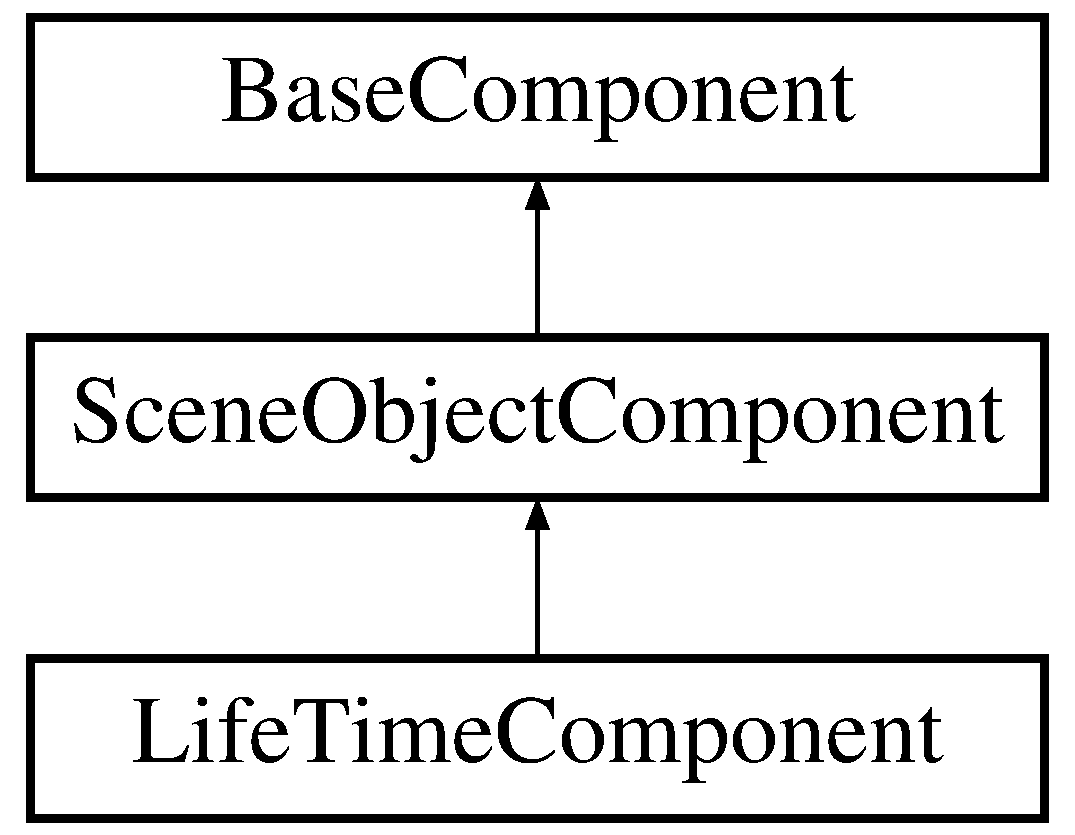
\includegraphics[height=3.000000cm]{class_life_time_component}
\end{center}
\end{figure}
\subsection*{Public Member Functions}
\begin{DoxyCompactItemize}
\item 
\hyperlink{class_life_time_component_a6021914ebabf59dce79b357790f1dbdb}{Life\+Time\+Component} (\hyperlink{class_scene_object}{Scene\+Object} $\ast$parent, std\+::weak\+\_\+ptr$<$ \hyperlink{class_meta_manager}{Meta\+Manager} $>$ managers, double life\+Span)
\begin{DoxyCompactList}\small\item\em Default constructor. \end{DoxyCompactList}\item 
virtual \hyperlink{class_life_time_component_a186edf6d26d61a244ec0893d3f927c57}{$\sim$\+Life\+Time\+Component} ()
\begin{DoxyCompactList}\small\item\em Default destructor. \end{DoxyCompactList}\item 
void \hyperlink{class_life_time_component_a709b9485f9bce5c7a6cec8f000bcb905}{step} (double dt) override
\begin{DoxyCompactList}\small\item\em Step the simulation state. \end{DoxyCompactList}\item 
void \hyperlink{class_life_time_component_a206515c60de0d9bc07062daf8d24446e}{predraw} (\hyperlink{class_context}{Context} $\ast$context) override
\begin{DoxyCompactList}\small\item\em Called before the renderer draws the scene This allows the scene objects to do updates that require a graphics context before the graphical state is drawn. \end{DoxyCompactList}\item 
void \hyperlink{class_life_time_component_a191771b06f2cf5c2b9bb2495e32c8ecf}{reset} ()
\begin{DoxyCompactList}\small\item\em Reset the timer to the original lifespan. \end{DoxyCompactList}\end{DoxyCompactItemize}
\subsection*{Private Attributes}
\begin{DoxyCompactItemize}
\item 
const double \hyperlink{class_life_time_component_adb6e05948b0edd9b4237861f064c9beb}{m\+\_\+\+Initial\+Life\+Span}
\begin{DoxyCompactList}\small\item\em The time to reset the lifespan to. \end{DoxyCompactList}\item 
double \hyperlink{class_life_time_component_a7a6b268136bb72e6b3d492d110681969}{m\+\_\+\+Life\+Span}
\begin{DoxyCompactList}\small\item\em Time before an object dies in seconds. \end{DoxyCompactList}\item 
bool \hyperlink{class_life_time_component_a9d1b78e698610ab263f788e29474b3bd}{m\+\_\+\+Triggered}
\begin{DoxyCompactList}\small\item\em True if the timeout has activated. \end{DoxyCompactList}\end{DoxyCompactItemize}
\subsection*{Additional Inherited Members}


\subsection{Detailed Description}
Attach to a scene object to give it a time limit to its existence. 

This is currently setup to use Axis-\/\+Aligned Bounding Boxes, but the collision subsystem for it has been gutted. \begin{DoxyRefDesc}{Todo}
\item[\hyperlink{todo__todo000002}{Todo}]Setup collision geometry\end{DoxyRefDesc}


\begin{DoxyAuthor}{Author}
Hayley Hatton 
\end{DoxyAuthor}
\begin{DoxyDate}{Date}
06/03/2016 
\end{DoxyDate}
\begin{DoxySeeAlso}{See also}
\hyperlink{class_collision_manager}{Collision\+Manager} 
\end{DoxySeeAlso}


Definition at line 16 of file Life\+Time\+Component.\+h.



\subsection{Constructor \& Destructor Documentation}
\index{Life\+Time\+Component@{Life\+Time\+Component}!Life\+Time\+Component@{Life\+Time\+Component}}
\index{Life\+Time\+Component@{Life\+Time\+Component}!Life\+Time\+Component@{Life\+Time\+Component}}
\subsubsection[{\texorpdfstring{Life\+Time\+Component(\+Scene\+Object $\ast$parent, std\+::weak\+\_\+ptr$<$ Meta\+Manager $>$ managers, double life\+Span)}{LifeTimeComponent(SceneObject *parent, std::weak_ptr< MetaManager > managers, double lifeSpan)}}]{\setlength{\rightskip}{0pt plus 5cm}Life\+Time\+Component\+::\+Life\+Time\+Component (
\begin{DoxyParamCaption}
\item[{{\bf Scene\+Object} $\ast$}]{parent, }
\item[{std\+::weak\+\_\+ptr$<$ {\bf Meta\+Manager} $>$}]{managers, }
\item[{double}]{life\+Span}
\end{DoxyParamCaption}
)}\hypertarget{class_life_time_component_a6021914ebabf59dce79b357790f1dbdb}{}\label{class_life_time_component_a6021914ebabf59dce79b357790f1dbdb}


Default constructor. 


\begin{DoxyParams}{Parameters}
{\em parent} & Pointer to the scene object to attach component to \\
\hline
{\em managers} & Metamanager for accessing scene\textquotesingle{}s managers \\
\hline
{\em life\+Span} & Time in seconds until the timeout is fired \\
\hline
\end{DoxyParams}


Definition at line 7 of file Life\+Time\+Component.\+cpp.

\index{Life\+Time\+Component@{Life\+Time\+Component}!````~Life\+Time\+Component@{$\sim$\+Life\+Time\+Component}}
\index{````~Life\+Time\+Component@{$\sim$\+Life\+Time\+Component}!Life\+Time\+Component@{Life\+Time\+Component}}
\subsubsection[{\texorpdfstring{$\sim$\+Life\+Time\+Component()}{~LifeTimeComponent()}}]{\setlength{\rightskip}{0pt plus 5cm}Life\+Time\+Component\+::$\sim$\+Life\+Time\+Component (
\begin{DoxyParamCaption}
{}
\end{DoxyParamCaption}
)\hspace{0.3cm}{\ttfamily [virtual]}}\hypertarget{class_life_time_component_a186edf6d26d61a244ec0893d3f927c57}{}\label{class_life_time_component_a186edf6d26d61a244ec0893d3f927c57}


Default destructor. 



Definition at line 18 of file Life\+Time\+Component.\+cpp.



\subsection{Member Function Documentation}
\index{Life\+Time\+Component@{Life\+Time\+Component}!predraw@{predraw}}
\index{predraw@{predraw}!Life\+Time\+Component@{Life\+Time\+Component}}
\subsubsection[{\texorpdfstring{predraw(\+Context $\ast$context) override}{predraw(Context *context) override}}]{\setlength{\rightskip}{0pt plus 5cm}void Life\+Time\+Component\+::predraw (
\begin{DoxyParamCaption}
\item[{{\bf Context} $\ast$}]{context}
\end{DoxyParamCaption}
)\hspace{0.3cm}{\ttfamily [inline]}, {\ttfamily [override]}, {\ttfamily [virtual]}}\hypertarget{class_life_time_component_a206515c60de0d9bc07062daf8d24446e}{}\label{class_life_time_component_a206515c60de0d9bc07062daf8d24446e}


Called before the renderer draws the scene This allows the scene objects to do updates that require a graphics context before the graphical state is drawn. 


\begin{DoxyParams}{Parameters}
{\em context} & Graphics context \\
\hline
\end{DoxyParams}


Implements \hyperlink{class_scene_object_component_a7110e37ad23a708c2bf9828c7fd7df2f}{Scene\+Object\+Component}.



Definition at line 47 of file Life\+Time\+Component.\+h.



References reset().

\index{Life\+Time\+Component@{Life\+Time\+Component}!reset@{reset}}
\index{reset@{reset}!Life\+Time\+Component@{Life\+Time\+Component}}
\subsubsection[{\texorpdfstring{reset()}{reset()}}]{\setlength{\rightskip}{0pt plus 5cm}void Life\+Time\+Component\+::reset (
\begin{DoxyParamCaption}
{}
\end{DoxyParamCaption}
)}\hypertarget{class_life_time_component_a191771b06f2cf5c2b9bb2495e32c8ecf}{}\label{class_life_time_component_a191771b06f2cf5c2b9bb2495e32c8ecf}


Reset the timer to the original lifespan. 



Definition at line 42 of file Life\+Time\+Component.\+cpp.



References m\+\_\+\+Initial\+Life\+Span, m\+\_\+\+Life\+Span, and m\+\_\+\+Triggered.



Referenced by predraw().

\index{Life\+Time\+Component@{Life\+Time\+Component}!step@{step}}
\index{step@{step}!Life\+Time\+Component@{Life\+Time\+Component}}
\subsubsection[{\texorpdfstring{step(double dt) override}{step(double dt) override}}]{\setlength{\rightskip}{0pt plus 5cm}void Life\+Time\+Component\+::step (
\begin{DoxyParamCaption}
\item[{double}]{dt}
\end{DoxyParamCaption}
)\hspace{0.3cm}{\ttfamily [override]}, {\ttfamily [virtual]}}\hypertarget{class_life_time_component_a709b9485f9bce5c7a6cec8f000bcb905}{}\label{class_life_time_component_a709b9485f9bce5c7a6cec8f000bcb905}


Step the simulation state. 


\begin{DoxyParams}{Parameters}
{\em dt} & Delta-\/time since last step call in seconds \\
\hline
\end{DoxyParams}


Implements \hyperlink{class_scene_object_component_a99ebed011a6547be4d31a09927e3b810}{Scene\+Object\+Component}.



Definition at line 23 of file Life\+Time\+Component.\+cpp.



References Scene\+Object\+Component\+::get\+Parent(), m\+\_\+\+Life\+Span, m\+\_\+\+Triggered, and I\+Message\+Listener\+::on\+Message().



\subsection{Member Data Documentation}
\index{Life\+Time\+Component@{Life\+Time\+Component}!m\+\_\+\+Initial\+Life\+Span@{m\+\_\+\+Initial\+Life\+Span}}
\index{m\+\_\+\+Initial\+Life\+Span@{m\+\_\+\+Initial\+Life\+Span}!Life\+Time\+Component@{Life\+Time\+Component}}
\subsubsection[{\texorpdfstring{m\+\_\+\+Initial\+Life\+Span}{m_InitialLifeSpan}}]{\setlength{\rightskip}{0pt plus 5cm}const double Life\+Time\+Component\+::m\+\_\+\+Initial\+Life\+Span\hspace{0.3cm}{\ttfamily [private]}}\hypertarget{class_life_time_component_adb6e05948b0edd9b4237861f064c9beb}{}\label{class_life_time_component_adb6e05948b0edd9b4237861f064c9beb}


The time to reset the lifespan to. 



Definition at line 53 of file Life\+Time\+Component.\+h.



Referenced by reset().

\index{Life\+Time\+Component@{Life\+Time\+Component}!m\+\_\+\+Life\+Span@{m\+\_\+\+Life\+Span}}
\index{m\+\_\+\+Life\+Span@{m\+\_\+\+Life\+Span}!Life\+Time\+Component@{Life\+Time\+Component}}
\subsubsection[{\texorpdfstring{m\+\_\+\+Life\+Span}{m_LifeSpan}}]{\setlength{\rightskip}{0pt plus 5cm}double Life\+Time\+Component\+::m\+\_\+\+Life\+Span\hspace{0.3cm}{\ttfamily [private]}}\hypertarget{class_life_time_component_a7a6b268136bb72e6b3d492d110681969}{}\label{class_life_time_component_a7a6b268136bb72e6b3d492d110681969}


Time before an object dies in seconds. 



Definition at line 54 of file Life\+Time\+Component.\+h.



Referenced by reset(), and step().

\index{Life\+Time\+Component@{Life\+Time\+Component}!m\+\_\+\+Triggered@{m\+\_\+\+Triggered}}
\index{m\+\_\+\+Triggered@{m\+\_\+\+Triggered}!Life\+Time\+Component@{Life\+Time\+Component}}
\subsubsection[{\texorpdfstring{m\+\_\+\+Triggered}{m_Triggered}}]{\setlength{\rightskip}{0pt plus 5cm}bool Life\+Time\+Component\+::m\+\_\+\+Triggered\hspace{0.3cm}{\ttfamily [private]}}\hypertarget{class_life_time_component_a9d1b78e698610ab263f788e29474b3bd}{}\label{class_life_time_component_a9d1b78e698610ab263f788e29474b3bd}


True if the timeout has activated. 



Definition at line 55 of file Life\+Time\+Component.\+h.



Referenced by reset(), and step().



The documentation for this class was generated from the following files\+:\begin{DoxyCompactItemize}
\item 
Lunar\+Drift/engine/components/\hyperlink{_life_time_component_8h}{Life\+Time\+Component.\+h}\item 
Lunar\+Drift/engine/components/\hyperlink{_life_time_component_8cpp}{Life\+Time\+Component.\+cpp}\end{DoxyCompactItemize}

\hypertarget{class_lunar_drift_program}{}\section{Lunar\+Drift\+Program Class Reference}
\label{class_lunar_drift_program}\index{Lunar\+Drift\+Program@{Lunar\+Drift\+Program}}


Top-\/level program class for our game.  




{\ttfamily \#include $<$Lunar\+Drift\+Program.\+h$>$}

Inheritance diagram for Lunar\+Drift\+Program\+:\begin{figure}[H]
\begin{center}
\leavevmode
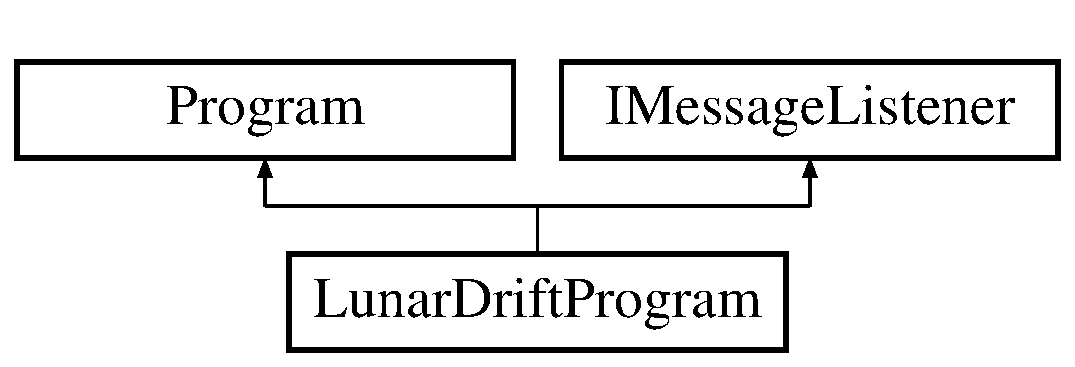
\includegraphics[height=2.000000cm]{class_lunar_drift_program}
\end{center}
\end{figure}
\subsection*{Public Member Functions}
\begin{DoxyCompactItemize}
\item 
\hyperlink{class_lunar_drift_program_aba4856c849b3972f4d31b1469789a81b}{Lunar\+Drift\+Program} (\hyperlink{class_context}{Context} $\ast$context)
\begin{DoxyCompactList}\small\item\em Object-\/oriented entry point to the program. \end{DoxyCompactList}\item 
\hyperlink{class_lunar_drift_program_a2729a6e9b131ad556a4d8b226c5d3a2e}{$\sim$\+Lunar\+Drift\+Program} ()
\begin{DoxyCompactList}\small\item\em Default destructor. \end{DoxyCompactList}\item 
void \hyperlink{class_lunar_drift_program_a3467aea42888a3eae28d587c90e5b1ff}{step} (double dt) override
\begin{DoxyCompactList}\small\item\em Called on the stepping of the simulation state. \end{DoxyCompactList}\item 
void \hyperlink{class_lunar_drift_program_a5db9835b135348644bc940cd7c2870be}{frame} (\hyperlink{class_context}{Context} $\ast$context) override
\begin{DoxyCompactList}\small\item\em Called on the rendering of a frame. \end{DoxyCompactList}\item 
void \hyperlink{class_lunar_drift_program_a6586725d0267426dae45c7c5772cffc2}{on\+Message} (std\+::shared\+\_\+ptr$<$ \hyperlink{class_message}{Message} $>$ event) override
\begin{DoxyCompactList}\small\item\em Called when a subscribed event is raised. \end{DoxyCompactList}\end{DoxyCompactItemize}
\subsection*{Static Public Attributes}
\begin{DoxyCompactItemize}
\item 
static const std\+::string \hyperlink{class_lunar_drift_program_a2b61915181711d5987e168c74d9beaac}{ms\+\_\+\+Name} = \char`\"{}Perpendicular\char`\"{}
\begin{DoxyCompactList}\small\item\em Name of the program. \end{DoxyCompactList}\end{DoxyCompactItemize}
\subsection*{Protected Member Functions}
\begin{DoxyCompactItemize}
\item 
std\+::shared\+\_\+ptr$<$ \hyperlink{class_renderer}{Renderer} $>$ \hyperlink{class_lunar_drift_program_a19fa2f0a909951f9e5cfdd7b5392be85}{get\+Renderer} (\hyperlink{class_context}{Context} $\ast$context) const  override
\begin{DoxyCompactList}\small\item\em Retrieve a new renderer for a given stereo mode from the subclass. \end{DoxyCompactList}\end{DoxyCompactItemize}


\subsection{Detailed Description}
Top-\/level program class for our game. 

\begin{DoxyAuthor}{Author}
Hayley Hatton 
\end{DoxyAuthor}
\begin{DoxyDate}{Date}
17/03/2016 
\end{DoxyDate}


Definition at line 12 of file Lunar\+Drift\+Program.\+h.



\subsection{Constructor \& Destructor Documentation}
\index{Lunar\+Drift\+Program@{Lunar\+Drift\+Program}!Lunar\+Drift\+Program@{Lunar\+Drift\+Program}}
\index{Lunar\+Drift\+Program@{Lunar\+Drift\+Program}!Lunar\+Drift\+Program@{Lunar\+Drift\+Program}}
\subsubsection[{\texorpdfstring{Lunar\+Drift\+Program(\+Context $\ast$context)}{LunarDriftProgram(Context *context)}}]{\setlength{\rightskip}{0pt plus 5cm}Lunar\+Drift\+Program\+::\+Lunar\+Drift\+Program (
\begin{DoxyParamCaption}
\item[{{\bf Context} $\ast$}]{context}
\end{DoxyParamCaption}
)}\hypertarget{class_lunar_drift_program_aba4856c849b3972f4d31b1469789a81b}{}\label{class_lunar_drift_program_aba4856c849b3972f4d31b1469789a81b}


Object-\/oriented entry point to the program. 


\begin{DoxyParams}{Parameters}
{\em context} & Graphics context \\
\hline
\end{DoxyParams}


Definition at line 10 of file Lunar\+Drift\+Program.\+cpp.



References Config\+::get(), Input\+Map\+::get\+Instance(), Input\+Map\+::get\+Keyboard(), Config\+::load(), Keyboard\+::map\+Key\+To\+Input(), Config\+::set(), and Program\+::set\+Active\+Scene().

\index{Lunar\+Drift\+Program@{Lunar\+Drift\+Program}!````~Lunar\+Drift\+Program@{$\sim$\+Lunar\+Drift\+Program}}
\index{````~Lunar\+Drift\+Program@{$\sim$\+Lunar\+Drift\+Program}!Lunar\+Drift\+Program@{Lunar\+Drift\+Program}}
\subsubsection[{\texorpdfstring{$\sim$\+Lunar\+Drift\+Program()}{~LunarDriftProgram()}}]{\setlength{\rightskip}{0pt plus 5cm}Lunar\+Drift\+Program\+::$\sim$\+Lunar\+Drift\+Program (
\begin{DoxyParamCaption}
{}
\end{DoxyParamCaption}
)}\hypertarget{class_lunar_drift_program_a2729a6e9b131ad556a4d8b226c5d3a2e}{}\label{class_lunar_drift_program_a2729a6e9b131ad556a4d8b226c5d3a2e}


Default destructor. 



Definition at line 24 of file Lunar\+Drift\+Program.\+cpp.



\subsection{Member Function Documentation}
\index{Lunar\+Drift\+Program@{Lunar\+Drift\+Program}!frame@{frame}}
\index{frame@{frame}!Lunar\+Drift\+Program@{Lunar\+Drift\+Program}}
\subsubsection[{\texorpdfstring{frame(\+Context $\ast$context) override}{frame(Context *context) override}}]{\setlength{\rightskip}{0pt plus 5cm}void Lunar\+Drift\+Program\+::frame (
\begin{DoxyParamCaption}
\item[{{\bf Context} $\ast$}]{context}
\end{DoxyParamCaption}
)\hspace{0.3cm}{\ttfamily [override]}, {\ttfamily [virtual]}}\hypertarget{class_lunar_drift_program_a5db9835b135348644bc940cd7c2870be}{}\label{class_lunar_drift_program_a5db9835b135348644bc940cd7c2870be}


Called on the rendering of a frame. 


\begin{DoxyParams}{Parameters}
{\em context} & Graphical context \\
\hline
\end{DoxyParams}


Reimplemented from \hyperlink{class_program_a3b02a58d4c366e280759bc8bbdd4b50d}{Program}.



Definition at line 35 of file Lunar\+Drift\+Program.\+cpp.



References Program\+::frame().

\index{Lunar\+Drift\+Program@{Lunar\+Drift\+Program}!get\+Renderer@{get\+Renderer}}
\index{get\+Renderer@{get\+Renderer}!Lunar\+Drift\+Program@{Lunar\+Drift\+Program}}
\subsubsection[{\texorpdfstring{get\+Renderer(\+Context $\ast$context) const  override}{getRenderer(Context *context) const  override}}]{\setlength{\rightskip}{0pt plus 5cm}std\+::shared\+\_\+ptr$<$ {\bf Renderer} $>$ Lunar\+Drift\+Program\+::get\+Renderer (
\begin{DoxyParamCaption}
\item[{{\bf Context} $\ast$}]{context}
\end{DoxyParamCaption}
) const\hspace{0.3cm}{\ttfamily [override]}, {\ttfamily [protected]}, {\ttfamily [virtual]}}\hypertarget{class_lunar_drift_program_a19fa2f0a909951f9e5cfdd7b5392be85}{}\label{class_lunar_drift_program_a19fa2f0a909951f9e5cfdd7b5392be85}


Retrieve a new renderer for a given stereo mode from the subclass. 

\begin{DoxyReturn}{Returns}
Smart pointer to the new appropriate renderer 
\end{DoxyReturn}


Implements \hyperlink{class_program_a016ef26d3d6b6aeffd3b4e74dfde033e}{Program}.



Definition at line 47 of file Lunar\+Drift\+Program.\+cpp.



References Context\+::get\+Dimensions(), h, and w.

\index{Lunar\+Drift\+Program@{Lunar\+Drift\+Program}!on\+Message@{on\+Message}}
\index{on\+Message@{on\+Message}!Lunar\+Drift\+Program@{Lunar\+Drift\+Program}}
\subsubsection[{\texorpdfstring{on\+Message(std\+::shared\+\_\+ptr$<$ Message $>$ event) override}{onMessage(std::shared_ptr< Message > event) override}}]{\setlength{\rightskip}{0pt plus 5cm}void Lunar\+Drift\+Program\+::on\+Message (
\begin{DoxyParamCaption}
\item[{std\+::shared\+\_\+ptr$<$ {\bf Message} $>$}]{event}
\end{DoxyParamCaption}
)\hspace{0.3cm}{\ttfamily [override]}, {\ttfamily [virtual]}}\hypertarget{class_lunar_drift_program_a6586725d0267426dae45c7c5772cffc2}{}\label{class_lunar_drift_program_a6586725d0267426dae45c7c5772cffc2}


Called when a subscribed event is raised. 


\begin{DoxyParams}{Parameters}
{\em event} & Smart pointer to the raised event object \\
\hline
\end{DoxyParams}


Implements \hyperlink{class_i_message_listener_aac85f64eeb587944c59e07f5457b1b82}{I\+Message\+Listener}.



Definition at line 43 of file Lunar\+Drift\+Program.\+cpp.

\index{Lunar\+Drift\+Program@{Lunar\+Drift\+Program}!step@{step}}
\index{step@{step}!Lunar\+Drift\+Program@{Lunar\+Drift\+Program}}
\subsubsection[{\texorpdfstring{step(double dt) override}{step(double dt) override}}]{\setlength{\rightskip}{0pt plus 5cm}void Lunar\+Drift\+Program\+::step (
\begin{DoxyParamCaption}
\item[{double}]{dt}
\end{DoxyParamCaption}
)\hspace{0.3cm}{\ttfamily [override]}, {\ttfamily [virtual]}}\hypertarget{class_lunar_drift_program_a3467aea42888a3eae28d587c90e5b1ff}{}\label{class_lunar_drift_program_a3467aea42888a3eae28d587c90e5b1ff}


Called on the stepping of the simulation state. 


\begin{DoxyParams}{Parameters}
{\em dt} & Delta time, in seconds \\
\hline
\end{DoxyParams}


Reimplemented from \hyperlink{class_program_a975de71413195823c525955cfd5f2ca7}{Program}.



Definition at line 30 of file Lunar\+Drift\+Program.\+cpp.



References Program\+::step().



\subsection{Member Data Documentation}
\index{Lunar\+Drift\+Program@{Lunar\+Drift\+Program}!ms\+\_\+\+Name@{ms\+\_\+\+Name}}
\index{ms\+\_\+\+Name@{ms\+\_\+\+Name}!Lunar\+Drift\+Program@{Lunar\+Drift\+Program}}
\subsubsection[{\texorpdfstring{ms\+\_\+\+Name}{ms_Name}}]{\setlength{\rightskip}{0pt plus 5cm}const std\+::string Lunar\+Drift\+Program\+::ms\+\_\+\+Name = \char`\"{}Perpendicular\char`\"{}\hspace{0.3cm}{\ttfamily [static]}}\hypertarget{class_lunar_drift_program_a2b61915181711d5987e168c74d9beaac}{}\label{class_lunar_drift_program_a2b61915181711d5987e168c74d9beaac}


Name of the program. 



Definition at line 45 of file Lunar\+Drift\+Program.\+h.



Referenced by Win\+Main().



The documentation for this class was generated from the following files\+:\begin{DoxyCompactItemize}
\item 
Lunar\+Drift/game/\hyperlink{_lunar_drift_program_8h}{Lunar\+Drift\+Program.\+h}\item 
Lunar\+Drift/game/\hyperlink{_lunar_drift_program_8cpp}{Lunar\+Drift\+Program.\+cpp}\end{DoxyCompactItemize}

\hypertarget{class_manager}{}\section{Manager Class Reference}
\label{class_manager}\index{Manager@{Manager}}


{\ttfamily \#include $<$Manager.\+h$>$}

Inheritance diagram for Manager\+:\begin{figure}[H]
\begin{center}
\leavevmode
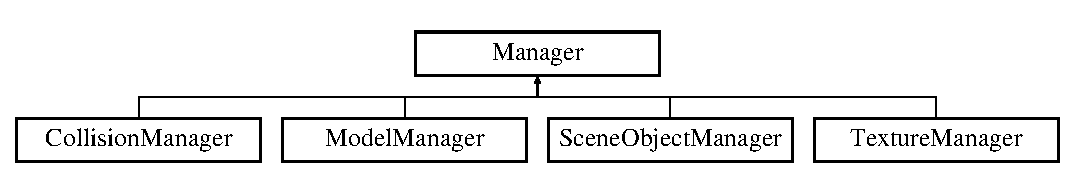
\includegraphics[height=1.944445cm]{class_manager}
\end{center}
\end{figure}
\subsection*{Public Member Functions}
\begin{DoxyCompactItemize}
\item 
\hyperlink{class_manager_ad9b5fb92579e44002e96f9df8fbdc984}{Manager} (const std\+::string \&name)
\item 
virtual \hyperlink{class_manager_a3dbc694b640c70009c5e0dec515d692c}{$\sim$\+Manager} ()
\item 
const std\+::string \& \hyperlink{class_manager_a842a5e896bd2bc7048f7580b5b7e0c7f}{get\+Manager\+Name} ()
\end{DoxyCompactItemize}
\subsection*{Private Attributes}
\begin{DoxyCompactItemize}
\item 
const std\+::string \hyperlink{class_manager_a746ab3e8df717773513e662ad7305259}{m\+\_\+\+Name}
\end{DoxyCompactItemize}


\subsection{Detailed Description}


Definition at line 5 of file Manager.\+h.



\subsection{Constructor \& Destructor Documentation}
\index{Manager@{Manager}!Manager@{Manager}}
\index{Manager@{Manager}!Manager@{Manager}}
\subsubsection[{\texorpdfstring{Manager(const std\+::string \&name)}{Manager(const std::string &name)}}]{\setlength{\rightskip}{0pt plus 5cm}Manager\+::\+Manager (
\begin{DoxyParamCaption}
\item[{const std\+::string \&}]{name}
\end{DoxyParamCaption}
)\hspace{0.3cm}{\ttfamily [inline]}}\hypertarget{class_manager_ad9b5fb92579e44002e96f9df8fbdc984}{}\label{class_manager_ad9b5fb92579e44002e96f9df8fbdc984}


Definition at line 8 of file Manager.\+h.

\index{Manager@{Manager}!````~Manager@{$\sim$\+Manager}}
\index{````~Manager@{$\sim$\+Manager}!Manager@{Manager}}
\subsubsection[{\texorpdfstring{$\sim$\+Manager()}{~Manager()}}]{\setlength{\rightskip}{0pt plus 5cm}virtual Manager\+::$\sim$\+Manager (
\begin{DoxyParamCaption}
{}
\end{DoxyParamCaption}
)\hspace{0.3cm}{\ttfamily [inline]}, {\ttfamily [virtual]}}\hypertarget{class_manager_a3dbc694b640c70009c5e0dec515d692c}{}\label{class_manager_a3dbc694b640c70009c5e0dec515d692c}


Definition at line 10 of file Manager.\+h.



\subsection{Member Function Documentation}
\index{Manager@{Manager}!get\+Manager\+Name@{get\+Manager\+Name}}
\index{get\+Manager\+Name@{get\+Manager\+Name}!Manager@{Manager}}
\subsubsection[{\texorpdfstring{get\+Manager\+Name()}{getManagerName()}}]{\setlength{\rightskip}{0pt plus 5cm}const std\+::string\& Manager\+::get\+Manager\+Name (
\begin{DoxyParamCaption}
{}
\end{DoxyParamCaption}
)\hspace{0.3cm}{\ttfamily [inline]}}\hypertarget{class_manager_a842a5e896bd2bc7048f7580b5b7e0c7f}{}\label{class_manager_a842a5e896bd2bc7048f7580b5b7e0c7f}


Definition at line 13 of file Manager.\+h.



References m\+\_\+\+Name.



\subsection{Member Data Documentation}
\index{Manager@{Manager}!m\+\_\+\+Name@{m\+\_\+\+Name}}
\index{m\+\_\+\+Name@{m\+\_\+\+Name}!Manager@{Manager}}
\subsubsection[{\texorpdfstring{m\+\_\+\+Name}{m_Name}}]{\setlength{\rightskip}{0pt plus 5cm}const std\+::string Manager\+::m\+\_\+\+Name\hspace{0.3cm}{\ttfamily [private]}}\hypertarget{class_manager_a746ab3e8df717773513e662ad7305259}{}\label{class_manager_a746ab3e8df717773513e662ad7305259}


Definition at line 16 of file Manager.\+h.



Referenced by get\+Manager\+Name().



The documentation for this class was generated from the following file\+:\begin{DoxyCompactItemize}
\item 
Lunar\+Drift/engine/managers/\hyperlink{_manager_8h}{Manager.\+h}\end{DoxyCompactItemize}

\hypertarget{class_message}{}\section{Message Class Reference}
\label{class_message}\index{Message@{Message}}


Base class for messages.  




{\ttfamily \#include $<$Message.\+h$>$}

Inheritance diagram for Message\+:\begin{figure}[H]
\begin{center}
\leavevmode
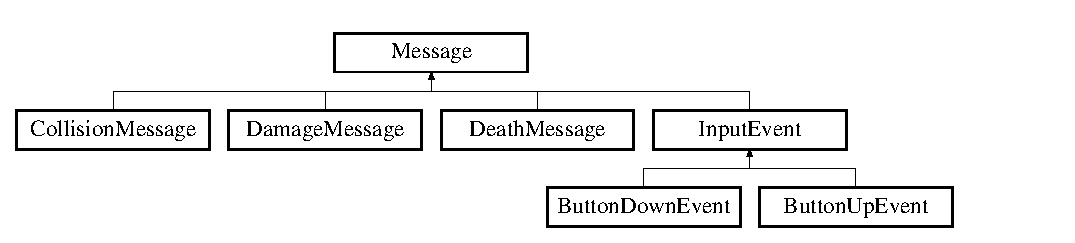
\includegraphics[height=2.823529cm]{class_message}
\end{center}
\end{figure}
\subsection*{Public Member Functions}
\begin{DoxyCompactItemize}
\item 
\hyperlink{class_message_a3092661fab5b2cca2405372abf68cd91}{Message} (const std\+::string \&type)
\begin{DoxyCompactList}\small\item\em Default constructor. \end{DoxyCompactList}\item 
virtual \hyperlink{class_message_a3f7275462831f787a861271687bcad67}{$\sim$\+Message} ()
\begin{DoxyCompactList}\small\item\em Default destructor. \end{DoxyCompactList}\item 
const std\+::string \& \hyperlink{class_message_af9a175efa065d40d7bc9903f6ba2cc5d}{get\+Type} () const 
\begin{DoxyCompactList}\small\item\em Access the type identifier of the derived message subclass. \end{DoxyCompactList}\end{DoxyCompactItemize}
\subsection*{Private Attributes}
\begin{DoxyCompactItemize}
\item 
const std\+::string \hyperlink{class_message_ae74bd8f969ef873186859fc3a7ad0e41}{m\+\_\+\+Type}
\begin{DoxyCompactList}\small\item\em Type identifier of the derived class. \end{DoxyCompactList}\end{DoxyCompactItemize}


\subsection{Detailed Description}
Base class for messages. 

Messages are packets of data sent between entities in the program. Events operate in a broadcast fashion, messages operate in a unicast fashion with a sender and a receiver at the point of handling.

\begin{DoxyAuthor}{Author}
Hayley Hatton 
\end{DoxyAuthor}
\begin{DoxyDate}{Date}
10/03/2016 
\end{DoxyDate}
\begin{DoxySeeAlso}{See also}
\hyperlink{class_i_message_listener}{I\+Message\+Listener} 

\hyperlink{class_message_system}{Message\+System} 
\end{DoxySeeAlso}


Definition at line 17 of file Message.\+h.



\subsection{Constructor \& Destructor Documentation}
\index{Message@{Message}!Message@{Message}}
\index{Message@{Message}!Message@{Message}}
\subsubsection[{\texorpdfstring{Message(const std\+::string \&type)}{Message(const std::string &type)}}]{\setlength{\rightskip}{0pt plus 5cm}Message\+::\+Message (
\begin{DoxyParamCaption}
\item[{const std\+::string \&}]{type}
\end{DoxyParamCaption}
)}\hypertarget{class_message_a3092661fab5b2cca2405372abf68cd91}{}\label{class_message_a3092661fab5b2cca2405372abf68cd91}


Default constructor. 


\begin{DoxyParams}{Parameters}
{\em type} & Type identifier string \\
\hline
\end{DoxyParams}


Definition at line 3 of file Message.\+cpp.

\index{Message@{Message}!````~Message@{$\sim$\+Message}}
\index{````~Message@{$\sim$\+Message}!Message@{Message}}
\subsubsection[{\texorpdfstring{$\sim$\+Message()}{~Message()}}]{\setlength{\rightskip}{0pt plus 5cm}Message\+::$\sim$\+Message (
\begin{DoxyParamCaption}
{}
\end{DoxyParamCaption}
)\hspace{0.3cm}{\ttfamily [virtual]}}\hypertarget{class_message_a3f7275462831f787a861271687bcad67}{}\label{class_message_a3f7275462831f787a861271687bcad67}


Default destructor. 



Definition at line 8 of file Message.\+cpp.



\subsection{Member Function Documentation}
\index{Message@{Message}!get\+Type@{get\+Type}}
\index{get\+Type@{get\+Type}!Message@{Message}}
\subsubsection[{\texorpdfstring{get\+Type() const }{getType() const }}]{\setlength{\rightskip}{0pt plus 5cm}const std\+::string\& Message\+::get\+Type (
\begin{DoxyParamCaption}
{}
\end{DoxyParamCaption}
) const\hspace{0.3cm}{\ttfamily [inline]}}\hypertarget{class_message_af9a175efa065d40d7bc9903f6ba2cc5d}{}\label{class_message_af9a175efa065d40d7bc9903f6ba2cc5d}


Access the type identifier of the derived message subclass. 

\begin{DoxyReturn}{Returns}
Type identifier string 
\end{DoxyReturn}


Definition at line 34 of file Message.\+h.



References m\+\_\+\+Type.



\subsection{Member Data Documentation}
\index{Message@{Message}!m\+\_\+\+Type@{m\+\_\+\+Type}}
\index{m\+\_\+\+Type@{m\+\_\+\+Type}!Message@{Message}}
\subsubsection[{\texorpdfstring{m\+\_\+\+Type}{m_Type}}]{\setlength{\rightskip}{0pt plus 5cm}const std\+::string Message\+::m\+\_\+\+Type\hspace{0.3cm}{\ttfamily [private]}}\hypertarget{class_message_ae74bd8f969ef873186859fc3a7ad0e41}{}\label{class_message_ae74bd8f969ef873186859fc3a7ad0e41}


Type identifier of the derived class. 



Definition at line 39 of file Message.\+h.



Referenced by get\+Type().



The documentation for this class was generated from the following files\+:\begin{DoxyCompactItemize}
\item 
Lunar\+Drift/engine/comms/\hyperlink{_message_8h}{Message.\+h}\item 
Lunar\+Drift/engine/comms/\hyperlink{_message_8cpp}{Message.\+cpp}\end{DoxyCompactItemize}

\hypertarget{class_message_system}{}\section{Message\+System Class Reference}
\label{class_message_system}\index{Message\+System@{Message\+System}}


Singletonized central processing system for messages and events.  




{\ttfamily \#include $<$Message\+System.\+h$>$}

\subsection*{Public Member Functions}
\begin{DoxyCompactItemize}
\item 
void \hyperlink{class_message_system_a91321ec1bf6906c05d3822da67a9c6bf}{register\+Listener} (const std\+::string \&name, \hyperlink{class_i_message_listener}{I\+Message\+Listener} $\ast$listener)
\begin{DoxyCompactList}\small\item\em Register a class instance as a message listener. \end{DoxyCompactList}\item 
void \hyperlink{class_message_system_accddc135ff948b8278d35463548327e2}{unregister\+Listener} (const std\+::string \&name)
\begin{DoxyCompactList}\small\item\em Unregister a message listener from being a listener. \end{DoxyCompactList}\item 
void \hyperlink{class_message_system_af555d4baae75e939aa5f388284138547}{unregister\+Listener} (\hyperlink{class_i_message_listener}{I\+Message\+Listener} $\ast$listener)
\begin{DoxyCompactList}\small\item\em Unregister a class instance from being a listener. \end{DoxyCompactList}\item 
void \hyperlink{class_message_system_aae34b407afa37e0a5b8c8eab0cf986b0}{subscribe} (const std\+::string \&sevent, \hyperlink{class_i_message_listener}{I\+Message\+Listener} $\ast$listener)
\begin{DoxyCompactList}\small\item\em Subscribe a class instance to receive events of a given name. \end{DoxyCompactList}\item 
void \hyperlink{class_message_system_a68fdb778ec79f4ddf25561d0e39b1c00}{unsubscribe} (const std\+::string \&sevent, \hyperlink{class_i_message_listener}{I\+Message\+Listener} $\ast$listener)
\begin{DoxyCompactList}\small\item\em Unsubscribe a class instance from receiving events of a given name. \end{DoxyCompactList}\item 
void \hyperlink{class_message_system_a2dc1a1964004d3133caea558b6e05f52}{broadcast} (std\+::shared\+\_\+ptr$<$ \hyperlink{class_message}{Message} $>$ event)
\begin{DoxyCompactList}\small\item\em Broadcast an event in the system to anyone interested. \end{DoxyCompactList}\item 
void \hyperlink{class_message_system_a13765245014da37033b0a3696425708a}{post} (const std\+::string \&to, std\+::shared\+\_\+ptr$<$ \hyperlink{class_message}{Message} $>$ msg)
\begin{DoxyCompactList}\small\item\em Post a message to a registered listener. \end{DoxyCompactList}\item 
void \hyperlink{class_message_system_a435432c27003a5d62b4a85811740cc33}{post} (\hyperlink{class_i_message_listener}{I\+Message\+Listener} $\ast$listener, std\+::shared\+\_\+ptr$<$ \hyperlink{class_message}{Message} $>$ msg)
\begin{DoxyCompactList}\small\item\em Post a message to a listener. \end{DoxyCompactList}\end{DoxyCompactItemize}
\subsection*{Static Public Member Functions}
\begin{DoxyCompactItemize}
\item 
static \hyperlink{class_message_system}{Message\+System} \& \hyperlink{class_message_system_a90338799a15b484765c4a8b94d140648}{get\+Instance} ()
\begin{DoxyCompactList}\small\item\em Singleton access. \end{DoxyCompactList}\end{DoxyCompactItemize}
\subsection*{Private Member Functions}
\begin{DoxyCompactItemize}
\item 
\hyperlink{class_message_system_ac7a164731432f7aa8bfadbc46008f777}{Message\+System} ()
\item 
\hyperlink{class_message_system_ab0bcc49967b11c9e34231972b44a22cd}{Message\+System} (\hyperlink{class_message_system}{Message\+System} const \&)=delete
\item 
void \hyperlink{class_message_system_adae1512cf046f08efff4b00244d80caf}{operator=} (\hyperlink{class_message_system}{Message\+System} const \&)=delete
\end{DoxyCompactItemize}
\subsection*{Private Attributes}
\begin{DoxyCompactItemize}
\item 
std\+::map$<$ std\+::string, \hyperlink{class_i_message_listener}{I\+Message\+Listener} $\ast$ $>$ \hyperlink{class_message_system_ab4b90cfd3e6e27a6ae7417ecf17123d7}{m\+\_\+\+Listeners}
\item 
std\+::map$<$ std\+::string, std\+::list$<$ \hyperlink{class_i_message_listener}{I\+Message\+Listener} $\ast$ $>$ $>$ \hyperlink{class_message_system_a64730035cb0e435bd3b1ff4c1c8dfe20}{m\+\_\+\+Subscribers}
\end{DoxyCompactItemize}


\subsection{Detailed Description}
Singletonized central processing system for messages and events. 

This singleton encapsulates communication between entities in the program. Events and messages are dispatched through this class for dispatching to the relevant entities. For understanding, imagine if you will the idea of a post office, wherein letters and newspapers are posted through; this class is that post office. Consequently, its responsibilities include holding information on \char`\"{}subscriptions\char`\"{} (who is subscribed to set events) and storing names and addresses of \char`\"{}listeners\char`\"{} (for posting messages to), and processing the dispatching of events and messages to those interested, respectively.

\begin{DoxyAuthor}{Author}
Hayley Hatton 
\end{DoxyAuthor}
\begin{DoxyDate}{Date}
10/03/2016 
\end{DoxyDate}
\begin{DoxySeeAlso}{See also}
\hyperlink{class_i_message_listener}{I\+Message\+Listener} 

\hyperlink{class_message}{Message} 
\end{DoxySeeAlso}


Definition at line 24 of file Message\+System.\+h.



\subsection{Constructor \& Destructor Documentation}
\index{Message\+System@{Message\+System}!Message\+System@{Message\+System}}
\index{Message\+System@{Message\+System}!Message\+System@{Message\+System}}
\subsubsection[{\texorpdfstring{Message\+System()}{MessageSystem()}}]{\setlength{\rightskip}{0pt plus 5cm}Message\+System\+::\+Message\+System (
\begin{DoxyParamCaption}
{}
\end{DoxyParamCaption}
)\hspace{0.3cm}{\ttfamily [inline]}, {\ttfamily [private]}}\hypertarget{class_message_system_ac7a164731432f7aa8bfadbc46008f777}{}\label{class_message_system_ac7a164731432f7aa8bfadbc46008f777}


Definition at line 99 of file Message\+System.\+h.



References operator=().

\index{Message\+System@{Message\+System}!Message\+System@{Message\+System}}
\index{Message\+System@{Message\+System}!Message\+System@{Message\+System}}
\subsubsection[{\texorpdfstring{Message\+System(\+Message\+System const \&)=delete}{MessageSystem(MessageSystem const &)=delete}}]{\setlength{\rightskip}{0pt plus 5cm}Message\+System\+::\+Message\+System (
\begin{DoxyParamCaption}
\item[{{\bf Message\+System} const \&}]{}
\end{DoxyParamCaption}
)\hspace{0.3cm}{\ttfamily [private]}, {\ttfamily [delete]}}\hypertarget{class_message_system_ab0bcc49967b11c9e34231972b44a22cd}{}\label{class_message_system_ab0bcc49967b11c9e34231972b44a22cd}


\subsection{Member Function Documentation}
\index{Message\+System@{Message\+System}!broadcast@{broadcast}}
\index{broadcast@{broadcast}!Message\+System@{Message\+System}}
\subsubsection[{\texorpdfstring{broadcast(std\+::shared\+\_\+ptr$<$ Message $>$ event)}{broadcast(std::shared_ptr< Message > event)}}]{\setlength{\rightskip}{0pt plus 5cm}void Message\+System\+::broadcast (
\begin{DoxyParamCaption}
\item[{std\+::shared\+\_\+ptr$<$ {\bf Message} $>$}]{event}
\end{DoxyParamCaption}
)}\hypertarget{class_message_system_a2dc1a1964004d3133caea558b6e05f52}{}\label{class_message_system_a2dc1a1964004d3133caea558b6e05f52}


Broadcast an event in the system to anyone interested. 


\begin{DoxyParams}{Parameters}
{\em event} & Smart pointer to event \\
\hline
\end{DoxyParams}


Definition at line 46 of file Message\+System.\+cpp.



References m\+\_\+\+Subscribers.



Referenced by get\+Instance(), Hitpoint\+Component\+::on\+Message(), Keyboard\+::set\+Key\+Down(), and Keyboard\+::set\+Key\+Up().

\index{Message\+System@{Message\+System}!get\+Instance@{get\+Instance}}
\index{get\+Instance@{get\+Instance}!Message\+System@{Message\+System}}
\subsubsection[{\texorpdfstring{get\+Instance()}{getInstance()}}]{\setlength{\rightskip}{0pt plus 5cm}static {\bf Message\+System}\& Message\+System\+::get\+Instance (
\begin{DoxyParamCaption}
{}
\end{DoxyParamCaption}
)\hspace{0.3cm}{\ttfamily [inline]}, {\ttfamily [static]}}\hypertarget{class_message_system_a90338799a15b484765c4a8b94d140648}{}\label{class_message_system_a90338799a15b484765c4a8b94d140648}


Singleton access. 



Definition at line 30 of file Message\+System.\+h.



References broadcast(), post(), register\+Listener(), subscribe(), unregister\+Listener(), and unsubscribe().



Referenced by Collision\+Component\+::\+Collision\+Component(), Hitpoint\+Component\+::\+Hitpoint\+Component(), Hitpoint\+Component\+::on\+Message(), Keyboard\+::set\+Key\+Down(), Keyboard\+::set\+Key\+Up(), Test\+Scene3\+D\+::\+Test\+Scene3\+D(), Test\+Triangle\+::\+Test\+Triangle(), Collision\+Component\+::$\sim$\+Collision\+Component(), Hitpoint\+Component\+::$\sim$\+Hitpoint\+Component(), and Test\+Triangle\+::$\sim$\+Test\+Triangle().

\index{Message\+System@{Message\+System}!operator=@{operator=}}
\index{operator=@{operator=}!Message\+System@{Message\+System}}
\subsubsection[{\texorpdfstring{operator=(\+Message\+System const \&)=delete}{operator=(MessageSystem const &)=delete}}]{\setlength{\rightskip}{0pt plus 5cm}void Message\+System\+::operator= (
\begin{DoxyParamCaption}
\item[{{\bf Message\+System} const \&}]{}
\end{DoxyParamCaption}
)\hspace{0.3cm}{\ttfamily [private]}, {\ttfamily [delete]}}\hypertarget{class_message_system_adae1512cf046f08efff4b00244d80caf}{}\label{class_message_system_adae1512cf046f08efff4b00244d80caf}


Referenced by Message\+System().

\index{Message\+System@{Message\+System}!post@{post}}
\index{post@{post}!Message\+System@{Message\+System}}
\subsubsection[{\texorpdfstring{post(const std\+::string \&to, std\+::shared\+\_\+ptr$<$ Message $>$ msg)}{post(const std::string &to, std::shared_ptr< Message > msg)}}]{\setlength{\rightskip}{0pt plus 5cm}void Message\+System\+::post (
\begin{DoxyParamCaption}
\item[{const std\+::string \&}]{to, }
\item[{std\+::shared\+\_\+ptr$<$ {\bf Message} $>$}]{msg}
\end{DoxyParamCaption}
)}\hypertarget{class_message_system_a13765245014da37033b0a3696425708a}{}\label{class_message_system_a13765245014da37033b0a3696425708a}


Post a message to a registered listener. 


\begin{DoxyParams}{Parameters}
{\em to} & Name of the registered listener \\
\hline
{\em msg} & Smart pointer to the message \\
\hline
\end{DoxyParams}


Definition at line 57 of file Message\+System.\+cpp.



References m\+\_\+\+Listeners.



Referenced by get\+Instance().

\index{Message\+System@{Message\+System}!post@{post}}
\index{post@{post}!Message\+System@{Message\+System}}
\subsubsection[{\texorpdfstring{post(\+I\+Message\+Listener $\ast$listener, std\+::shared\+\_\+ptr$<$ Message $>$ msg)}{post(IMessageListener *listener, std::shared_ptr< Message > msg)}}]{\setlength{\rightskip}{0pt plus 5cm}void Message\+System\+::post (
\begin{DoxyParamCaption}
\item[{{\bf I\+Message\+Listener} $\ast$}]{listener, }
\item[{std\+::shared\+\_\+ptr$<$ {\bf Message} $>$}]{msg}
\end{DoxyParamCaption}
)}\hypertarget{class_message_system_a435432c27003a5d62b4a85811740cc33}{}\label{class_message_system_a435432c27003a5d62b4a85811740cc33}


Post a message to a listener. 


\begin{DoxyParams}{Parameters}
{\em listener} & Pointer to the listener \\
\hline
{\em msg} & Smart pointer to the message \\
\hline
\end{DoxyParams}


Definition at line 62 of file Message\+System.\+cpp.

\index{Message\+System@{Message\+System}!register\+Listener@{register\+Listener}}
\index{register\+Listener@{register\+Listener}!Message\+System@{Message\+System}}
\subsubsection[{\texorpdfstring{register\+Listener(const std\+::string \&name, I\+Message\+Listener $\ast$listener)}{registerListener(const std::string &name, IMessageListener *listener)}}]{\setlength{\rightskip}{0pt plus 5cm}void Message\+System\+::register\+Listener (
\begin{DoxyParamCaption}
\item[{const std\+::string \&}]{name, }
\item[{{\bf I\+Message\+Listener} $\ast$}]{listener}
\end{DoxyParamCaption}
)}\hypertarget{class_message_system_a91321ec1bf6906c05d3822da67a9c6bf}{}\label{class_message_system_a91321ec1bf6906c05d3822da67a9c6bf}


Register a class instance as a message listener. 


\begin{DoxyParams}{Parameters}
{\em name} & Name for posting messages to \\
\hline
{\em listener} & Pointer to class instance \\
\hline
\end{DoxyParams}


Definition at line 3 of file Message\+System.\+cpp.



References m\+\_\+\+Listeners.



Referenced by get\+Instance().

\index{Message\+System@{Message\+System}!subscribe@{subscribe}}
\index{subscribe@{subscribe}!Message\+System@{Message\+System}}
\subsubsection[{\texorpdfstring{subscribe(const std\+::string \&sevent, I\+Message\+Listener $\ast$listener)}{subscribe(const std::string &sevent, IMessageListener *listener)}}]{\setlength{\rightskip}{0pt plus 5cm}void Message\+System\+::subscribe (
\begin{DoxyParamCaption}
\item[{const std\+::string \&}]{sevent, }
\item[{{\bf I\+Message\+Listener} $\ast$}]{listener}
\end{DoxyParamCaption}
)}\hypertarget{class_message_system_aae34b407afa37e0a5b8c8eab0cf986b0}{}\label{class_message_system_aae34b407afa37e0a5b8c8eab0cf986b0}


Subscribe a class instance to receive events of a given name. 


\begin{DoxyParams}{Parameters}
{\em sevent} & Event name to subscribe to \\
\hline
{\em listener} & Pointer to the class instance \\
\hline
\end{DoxyParams}


Definition at line 26 of file Message\+System.\+cpp.



References m\+\_\+\+Subscribers.



Referenced by Collision\+Component\+::\+Collision\+Component(), get\+Instance(), Hitpoint\+Component\+::\+Hitpoint\+Component(), Test\+Scene3\+D\+::\+Test\+Scene3\+D(), and Test\+Triangle\+::\+Test\+Triangle().

\index{Message\+System@{Message\+System}!unregister\+Listener@{unregister\+Listener}}
\index{unregister\+Listener@{unregister\+Listener}!Message\+System@{Message\+System}}
\subsubsection[{\texorpdfstring{unregister\+Listener(const std\+::string \&name)}{unregisterListener(const std::string &name)}}]{\setlength{\rightskip}{0pt plus 5cm}void Message\+System\+::unregister\+Listener (
\begin{DoxyParamCaption}
\item[{const std\+::string \&}]{name}
\end{DoxyParamCaption}
)}\hypertarget{class_message_system_accddc135ff948b8278d35463548327e2}{}\label{class_message_system_accddc135ff948b8278d35463548327e2}


Unregister a message listener from being a listener. 


\begin{DoxyParams}{Parameters}
{\em name} & Name of the listener \\
\hline
\end{DoxyParams}


Definition at line 10 of file Message\+System.\+cpp.



References m\+\_\+\+Listeners.



Referenced by get\+Instance().

\index{Message\+System@{Message\+System}!unregister\+Listener@{unregister\+Listener}}
\index{unregister\+Listener@{unregister\+Listener}!Message\+System@{Message\+System}}
\subsubsection[{\texorpdfstring{unregister\+Listener(\+I\+Message\+Listener $\ast$listener)}{unregisterListener(IMessageListener *listener)}}]{\setlength{\rightskip}{0pt plus 5cm}void Message\+System\+::unregister\+Listener (
\begin{DoxyParamCaption}
\item[{{\bf I\+Message\+Listener} $\ast$}]{listener}
\end{DoxyParamCaption}
)}\hypertarget{class_message_system_af555d4baae75e939aa5f388284138547}{}\label{class_message_system_af555d4baae75e939aa5f388284138547}


Unregister a class instance from being a listener. 


\begin{DoxyParams}{Parameters}
{\em listener} & Class instance pointer \\
\hline
\end{DoxyParams}


Definition at line 15 of file Message\+System.\+cpp.



References m\+\_\+\+Listeners.

\index{Message\+System@{Message\+System}!unsubscribe@{unsubscribe}}
\index{unsubscribe@{unsubscribe}!Message\+System@{Message\+System}}
\subsubsection[{\texorpdfstring{unsubscribe(const std\+::string \&sevent, I\+Message\+Listener $\ast$listener)}{unsubscribe(const std::string &sevent, IMessageListener *listener)}}]{\setlength{\rightskip}{0pt plus 5cm}void Message\+System\+::unsubscribe (
\begin{DoxyParamCaption}
\item[{const std\+::string \&}]{sevent, }
\item[{{\bf I\+Message\+Listener} $\ast$}]{listener}
\end{DoxyParamCaption}
)}\hypertarget{class_message_system_a68fdb778ec79f4ddf25561d0e39b1c00}{}\label{class_message_system_a68fdb778ec79f4ddf25561d0e39b1c00}


Unsubscribe a class instance from receiving events of a given name. 


\begin{DoxyParams}{Parameters}
{\em sevent} & Event name to unsubscribe from \\
\hline
{\em listener} & Pointer to the class instance \\
\hline
\end{DoxyParams}


Definition at line 39 of file Message\+System.\+cpp.



References m\+\_\+\+Subscribers.



Referenced by get\+Instance(), Collision\+Component\+::$\sim$\+Collision\+Component(), Hitpoint\+Component\+::$\sim$\+Hitpoint\+Component(), and Test\+Triangle\+::$\sim$\+Test\+Triangle().



\subsection{Member Data Documentation}
\index{Message\+System@{Message\+System}!m\+\_\+\+Listeners@{m\+\_\+\+Listeners}}
\index{m\+\_\+\+Listeners@{m\+\_\+\+Listeners}!Message\+System@{Message\+System}}
\subsubsection[{\texorpdfstring{m\+\_\+\+Listeners}{m_Listeners}}]{\setlength{\rightskip}{0pt plus 5cm}std\+::map$<$std\+::string, {\bf I\+Message\+Listener}$\ast$$>$ Message\+System\+::m\+\_\+\+Listeners\hspace{0.3cm}{\ttfamily [private]}}\hypertarget{class_message_system_ab4b90cfd3e6e27a6ae7417ecf17123d7}{}\label{class_message_system_ab4b90cfd3e6e27a6ae7417ecf17123d7}


Definition at line 103 of file Message\+System.\+h.



Referenced by post(), register\+Listener(), and unregister\+Listener().

\index{Message\+System@{Message\+System}!m\+\_\+\+Subscribers@{m\+\_\+\+Subscribers}}
\index{m\+\_\+\+Subscribers@{m\+\_\+\+Subscribers}!Message\+System@{Message\+System}}
\subsubsection[{\texorpdfstring{m\+\_\+\+Subscribers}{m_Subscribers}}]{\setlength{\rightskip}{0pt plus 5cm}std\+::map$<$std\+::string, std\+::list$<${\bf I\+Message\+Listener}$\ast$$>$ $>$ Message\+System\+::m\+\_\+\+Subscribers\hspace{0.3cm}{\ttfamily [private]}}\hypertarget{class_message_system_a64730035cb0e435bd3b1ff4c1c8dfe20}{}\label{class_message_system_a64730035cb0e435bd3b1ff4c1c8dfe20}


Definition at line 104 of file Message\+System.\+h.



Referenced by broadcast(), subscribe(), and unsubscribe().



The documentation for this class was generated from the following files\+:\begin{DoxyCompactItemize}
\item 
Lunar\+Drift/engine/comms/\hyperlink{_message_system_8h}{Message\+System.\+h}\item 
Lunar\+Drift/engine/comms/\hyperlink{_message_system_8cpp}{Message\+System.\+cpp}\end{DoxyCompactItemize}

\hypertarget{class_meta_manager}{}\section{Meta\+Manager Class Reference}
\label{class_meta_manager}\index{Meta\+Manager@{Meta\+Manager}}


A manager class for managing and passing around managers.  




{\ttfamily \#include $<$Meta\+Manager.\+h$>$}

\subsection*{Public Member Functions}
\begin{DoxyCompactItemize}
\item 
\hyperlink{class_meta_manager_a7f75a78a1470d64c7e3caf41644061c5}{Meta\+Manager} ()
\begin{DoxyCompactList}\small\item\em Default constructor. \end{DoxyCompactList}\item 
virtual \hyperlink{class_meta_manager_ad0b66bed6144ddc320d2c5930046ab73}{$\sim$\+Meta\+Manager} ()
\begin{DoxyCompactList}\small\item\em Default destructor. \end{DoxyCompactList}\item 
void \hyperlink{class_meta_manager_a3b1c68062b4591c10a5fbcb1550e50d6}{add} (std\+::shared\+\_\+ptr$<$ \hyperlink{class_manager}{Manager} $>$ manager)
\begin{DoxyCompactList}\small\item\em Add a manager to be managed by the metamanager. \end{DoxyCompactList}\item 
void \hyperlink{class_meta_manager_a3de340f9eec8f318b53088f7633e68cd}{remove} (const std\+::string \&name)
\begin{DoxyCompactList}\small\item\em Remove a manager from the metamanager, if it exists. \end{DoxyCompactList}\item 
std\+::weak\+\_\+ptr$<$ \hyperlink{class_manager}{Manager} $>$ \hyperlink{class_meta_manager_a7e2c87f000842d51f835a9831a950332}{get} (const std\+::string \&name)
\begin{DoxyCompactList}\small\item\em Access a manager managed by the metamanager. \end{DoxyCompactList}\end{DoxyCompactItemize}
\subsection*{Private Attributes}
\begin{DoxyCompactItemize}
\item 
std\+::map$<$ std\+::string, std\+::shared\+\_\+ptr$<$ \hyperlink{class_manager}{Manager} $>$ $>$ \hyperlink{class_meta_manager_a5b914ef44240c7fa97778b2240c318e3}{m\+\_\+\+Managers}
\end{DoxyCompactItemize}


\subsection{Detailed Description}
A manager class for managing and passing around managers. 

\begin{DoxyAuthor}{Author}
Hayley Hatton 
\end{DoxyAuthor}
\begin{DoxyDate}{Date}
13/03/2016 
\end{DoxyDate}
\begin{DoxySeeAlso}{See also}
\hyperlink{class_manager}{Manager} 
\end{DoxySeeAlso}


Definition at line 14 of file Meta\+Manager.\+h.



\subsection{Constructor \& Destructor Documentation}
\index{Meta\+Manager@{Meta\+Manager}!Meta\+Manager@{Meta\+Manager}}
\index{Meta\+Manager@{Meta\+Manager}!Meta\+Manager@{Meta\+Manager}}
\subsubsection[{\texorpdfstring{Meta\+Manager()}{MetaManager()}}]{\setlength{\rightskip}{0pt plus 5cm}Meta\+Manager\+::\+Meta\+Manager (
\begin{DoxyParamCaption}
{}
\end{DoxyParamCaption}
)}\hypertarget{class_meta_manager_a7f75a78a1470d64c7e3caf41644061c5}{}\label{class_meta_manager_a7f75a78a1470d64c7e3caf41644061c5}


Default constructor. 



Definition at line 5 of file Meta\+Manager.\+cpp.

\index{Meta\+Manager@{Meta\+Manager}!````~Meta\+Manager@{$\sim$\+Meta\+Manager}}
\index{````~Meta\+Manager@{$\sim$\+Meta\+Manager}!Meta\+Manager@{Meta\+Manager}}
\subsubsection[{\texorpdfstring{$\sim$\+Meta\+Manager()}{~MetaManager()}}]{\setlength{\rightskip}{0pt plus 5cm}Meta\+Manager\+::$\sim$\+Meta\+Manager (
\begin{DoxyParamCaption}
{}
\end{DoxyParamCaption}
)\hspace{0.3cm}{\ttfamily [virtual]}}\hypertarget{class_meta_manager_ad0b66bed6144ddc320d2c5930046ab73}{}\label{class_meta_manager_ad0b66bed6144ddc320d2c5930046ab73}


Default destructor. 



Definition at line 9 of file Meta\+Manager.\+cpp.



\subsection{Member Function Documentation}
\index{Meta\+Manager@{Meta\+Manager}!add@{add}}
\index{add@{add}!Meta\+Manager@{Meta\+Manager}}
\subsubsection[{\texorpdfstring{add(std\+::shared\+\_\+ptr$<$ Manager $>$ manager)}{add(std::shared_ptr< Manager > manager)}}]{\setlength{\rightskip}{0pt plus 5cm}void Meta\+Manager\+::add (
\begin{DoxyParamCaption}
\item[{std\+::shared\+\_\+ptr$<$ {\bf Manager} $>$}]{manager}
\end{DoxyParamCaption}
)}\hypertarget{class_meta_manager_a3b1c68062b4591c10a5fbcb1550e50d6}{}\label{class_meta_manager_a3b1c68062b4591c10a5fbcb1550e50d6}


Add a manager to be managed by the metamanager. 


\begin{DoxyParams}{Parameters}
{\em manager} & Smart ptr to the manager to handle \\
\hline
\end{DoxyParams}


Definition at line 14 of file Meta\+Manager.\+cpp.



References m\+\_\+\+Managers.

\index{Meta\+Manager@{Meta\+Manager}!get@{get}}
\index{get@{get}!Meta\+Manager@{Meta\+Manager}}
\subsubsection[{\texorpdfstring{get(const std\+::string \&name)}{get(const std::string &name)}}]{\setlength{\rightskip}{0pt plus 5cm}std\+::weak\+\_\+ptr$<$ {\bf Manager} $>$ Meta\+Manager\+::get (
\begin{DoxyParamCaption}
\item[{const std\+::string \&}]{name}
\end{DoxyParamCaption}
)}\hypertarget{class_meta_manager_a7e2c87f000842d51f835a9831a950332}{}\label{class_meta_manager_a7e2c87f000842d51f835a9831a950332}


Access a manager managed by the metamanager. 


\begin{DoxyParams}{Parameters}
{\em name} & Identifier name of the manager to acquire \\
\hline
\end{DoxyParams}
\begin{DoxyReturn}{Returns}
Weakly managed ptr to the manager; nullptr if not available 
\end{DoxyReturn}


Definition at line 25 of file Meta\+Manager.\+cpp.



References m\+\_\+\+Managers.

\index{Meta\+Manager@{Meta\+Manager}!remove@{remove}}
\index{remove@{remove}!Meta\+Manager@{Meta\+Manager}}
\subsubsection[{\texorpdfstring{remove(const std\+::string \&name)}{remove(const std::string &name)}}]{\setlength{\rightskip}{0pt plus 5cm}void Meta\+Manager\+::remove (
\begin{DoxyParamCaption}
\item[{const std\+::string \&}]{name}
\end{DoxyParamCaption}
)}\hypertarget{class_meta_manager_a3de340f9eec8f318b53088f7633e68cd}{}\label{class_meta_manager_a3de340f9eec8f318b53088f7633e68cd}


Remove a manager from the metamanager, if it exists. 


\begin{DoxyParams}{Parameters}
{\em name} & Identifier name of the manager to remove \\
\hline
\end{DoxyParams}


Definition at line 20 of file Meta\+Manager.\+cpp.



References m\+\_\+\+Managers.



\subsection{Member Data Documentation}
\index{Meta\+Manager@{Meta\+Manager}!m\+\_\+\+Managers@{m\+\_\+\+Managers}}
\index{m\+\_\+\+Managers@{m\+\_\+\+Managers}!Meta\+Manager@{Meta\+Manager}}
\subsubsection[{\texorpdfstring{m\+\_\+\+Managers}{m_Managers}}]{\setlength{\rightskip}{0pt plus 5cm}std\+::map$<$std\+::string, std\+::shared\+\_\+ptr$<${\bf Manager}$>$ $>$ Meta\+Manager\+::m\+\_\+\+Managers\hspace{0.3cm}{\ttfamily [private]}}\hypertarget{class_meta_manager_a5b914ef44240c7fa97778b2240c318e3}{}\label{class_meta_manager_a5b914ef44240c7fa97778b2240c318e3}


Definition at line 44 of file Meta\+Manager.\+h.



Referenced by add(), get(), and remove().



The documentation for this class was generated from the following files\+:\begin{DoxyCompactItemize}
\item 
Lunar\+Drift/engine/managers/\hyperlink{_meta_manager_8h}{Meta\+Manager.\+h}\item 
Lunar\+Drift/engine/managers/\hyperlink{_meta_manager_8cpp}{Meta\+Manager.\+cpp}\end{DoxyCompactItemize}

\hypertarget{class_model}{}\section{Model Class Reference}
\label{class_model}\index{Model@{Model}}


Container for and loader of \char`\"{}model data\char`\"{} (a combination of vertex and texture data)  




{\ttfamily \#include $<$Model.\+h$>$}

\subsection*{Classes}
\begin{DoxyCompactItemize}
\item 
struct \hyperlink{struct_model_1_1_vertex}{Vertex}
\begin{DoxyCompactList}\small\item\em Predefined vertex format for standard 3D models. \end{DoxyCompactList}\end{DoxyCompactItemize}
\subsection*{Public Member Functions}
\begin{DoxyCompactItemize}
\item 
\hyperlink{class_model_abdd56a8ab376bfaad4ba8f19a06bebfb}{Model} (\hyperlink{class_context}{Context} $\ast$context, const std\+::string \&path)
\begin{DoxyCompactList}\small\item\em Constructor for loading a model from an O\+BJ file. \end{DoxyCompactList}\item 
\hyperlink{class_model_afcac6a00d14c867c891fbdcab4b39bc2}{Model} (\hyperlink{class_context}{Context} $\ast$context, const std\+::vector$<$ \hyperlink{struct_model_1_1_vertex}{Vertex} $>$ \&vertices)
\begin{DoxyCompactList}\small\item\em Constructor for a model using predefined vertex list. \end{DoxyCompactList}\item 
\hyperlink{class_model_aeea356baee526151b46b30f86c158a10}{Model} (\hyperlink{class_context}{Context} $\ast$context, const std\+::vector$<$ \hyperlink{struct_model_1_1_vertex}{Vertex} $>$ \&vertices, const std\+::vector$<$ unsigned short $>$ \&indices)
\begin{DoxyCompactList}\small\item\em Constructor for a model using predefined vertex and index lists. \end{DoxyCompactList}\item 
\hyperlink{class_model_ad6ebd2062a0b823db841a0b88baac4c0}{$\sim$\+Model} ()
\begin{DoxyCompactList}\small\item\em Default destructor. \end{DoxyCompactList}\item 
void \hyperlink{class_model_afb320a52ec7f8f8512eb6514cfc58848}{draw} (\hyperlink{class_context}{Context} $\ast$context, std\+::shared\+\_\+ptr$<$ \hyperlink{class_shader_program}{Shader\+Program} $>$ shader) const 
\begin{DoxyCompactList}\small\item\em Draw the model using a given shader. \end{DoxyCompactList}\item 
void \hyperlink{class_model_a07d55d70f3ec47d819e6ea75410ceb19}{set\+Primitive\+Mode} (\hyperlink{_model_8h_a8e9638a65349c0abba4e6b97c8251994}{Primitive\+Mode} mode)
\begin{DoxyCompactList}\small\item\em Set the typology of the model geometry for rendering. \end{DoxyCompactList}\item 
void \hyperlink{class_model_ade683835b46ca563594c0ff243ec5f1f}{set\+Vertex\+Array\+Object} (std\+::shared\+\_\+ptr$<$ \hyperlink{class_vertex_array_object}{Vertex\+Array\+Object} $>$ vao)
\begin{DoxyCompactList}\small\item\em Associate a given vertex array object with the model. \end{DoxyCompactList}\item 
std\+::weak\+\_\+ptr$<$ \hyperlink{class_vertex_array_object}{Vertex\+Array\+Object} $>$ \hyperlink{class_model_aabc7313d8e1160762a3d59584724fd2e}{get\+Vertex\+Array\+Object} () const 
\begin{DoxyCompactList}\small\item\em Access associated vertex array object. \end{DoxyCompactList}\end{DoxyCompactItemize}
\subsection*{Private Member Functions}
\begin{DoxyCompactItemize}
\item 
void \hyperlink{class_model_a5d5259d9548f9aae5562f3ecbb2803dc}{transfer\+To\+G\+PU} (\hyperlink{class_context}{Context} $\ast$context, const std\+::vector$<$ \hyperlink{struct_model_1_1_vertex}{Vertex} $>$ \&vertices, const std\+::vector$<$ unsigned short $>$ $\ast$const indices=nullptr)
\begin{DoxyCompactList}\small\item\em Compile model data into Open\+GL objects for managing them G\+P\+U-\/side. \end{DoxyCompactList}\item 
void \hyperlink{class_model_a26c6176bfee61caddc5e11180f9d3741}{get\+Vertex\+Attributes} (std\+::vector$<$ \hyperlink{class_vertex_attribute}{Vertex\+Attribute} $>$ $\ast$attribs) const 
\begin{DoxyCompactList}\small\item\em Fill a vector with vertex attributes to map the inputs to shaders. \end{DoxyCompactList}\end{DoxyCompactItemize}
\subsection*{Private Attributes}
\begin{DoxyCompactItemize}
\item 
std\+::shared\+\_\+ptr$<$ \hyperlink{class_vertex_array_object}{Vertex\+Array\+Object} $>$ \hyperlink{class_model_a33ddd71b6e11029a482f8fd0786d064d}{m\+\_\+\+V\+AO}
\begin{DoxyCompactList}\small\item\em Associated vertex array object. \end{DoxyCompactList}\item 
\hyperlink{_model_8h_a8e9638a65349c0abba4e6b97c8251994}{Primitive\+Mode} \hyperlink{class_model_af07134f1b940eb354fa85c3524d70411}{m\+\_\+\+Primitive\+Mode}
\begin{DoxyCompactList}\small\item\em Typology of the model geometry. \end{DoxyCompactList}\end{DoxyCompactItemize}


\subsection{Detailed Description}
Container for and loader of \char`\"{}model data\char`\"{} (a combination of vertex and texture data) 

\begin{DoxyPrecond}{Precondition}
A valid Open\+GL context must be present to the program 
\end{DoxyPrecond}
\begin{DoxyAuthor}{Author}
Hayley Hatton 
\end{DoxyAuthor}
\begin{DoxyDate}{Date}
06/03/2016 
\end{DoxyDate}
\begin{DoxySeeAlso}{See also}
\hyperlink{class_vertex_buffer_object}{Vertex\+Buffer\+Object} 

\hyperlink{class_shader_program}{Shader\+Program} 

\hyperlink{class_texture}{Texture} 

\hyperlink{class_vertex_array_object}{Vertex\+Array\+Object} 
\end{DoxySeeAlso}


Definition at line 34 of file Model.\+h.



\subsection{Constructor \& Destructor Documentation}
\index{Model@{Model}!Model@{Model}}
\index{Model@{Model}!Model@{Model}}
\subsubsection[{\texorpdfstring{Model(\+Context $\ast$context, const std\+::string \&path)}{Model(Context *context, const std::string &path)}}]{\setlength{\rightskip}{0pt plus 5cm}Model\+::\+Model (
\begin{DoxyParamCaption}
\item[{{\bf Context} $\ast$}]{context, }
\item[{const std\+::string \&}]{path}
\end{DoxyParamCaption}
)}\hypertarget{class_model_abdd56a8ab376bfaad4ba8f19a06bebfb}{}\label{class_model_abdd56a8ab376bfaad4ba8f19a06bebfb}


Constructor for loading a model from an O\+BJ file. 


\begin{DoxyParams}{Parameters}
{\em context} & Graphical context \\
\hline
{\em path} & Path to the O\+BJ file to load model data from \\
\hline
\end{DoxyParams}


Definition at line 7 of file Model.\+cpp.



References Model\+Loader\+::compile(), Model\+Loader\+::get\+Num\+Vertices(), transfer\+To\+G\+P\+U(), and Triangles.

\index{Model@{Model}!Model@{Model}}
\index{Model@{Model}!Model@{Model}}
\subsubsection[{\texorpdfstring{Model(\+Context $\ast$context, const std\+::vector$<$ Vertex $>$ \&vertices)}{Model(Context *context, const std::vector< Vertex > &vertices)}}]{\setlength{\rightskip}{0pt plus 5cm}Model\+::\+Model (
\begin{DoxyParamCaption}
\item[{{\bf Context} $\ast$}]{context, }
\item[{const std\+::vector$<$ {\bf Vertex} $>$ \&}]{vertices}
\end{DoxyParamCaption}
)}\hypertarget{class_model_afcac6a00d14c867c891fbdcab4b39bc2}{}\label{class_model_afcac6a00d14c867c891fbdcab4b39bc2}


Constructor for a model using predefined vertex list. 


\begin{DoxyParams}{Parameters}
{\em context} & Graphical context \\
\hline
{\em vertices} & List of vertices to make model from \\
\hline
\end{DoxyParams}


Definition at line 33 of file Model.\+cpp.



References transfer\+To\+G\+P\+U().

\index{Model@{Model}!Model@{Model}}
\index{Model@{Model}!Model@{Model}}
\subsubsection[{\texorpdfstring{Model(\+Context $\ast$context, const std\+::vector$<$ Vertex $>$ \&vertices, const std\+::vector$<$ unsigned short $>$ \&indices)}{Model(Context *context, const std::vector< Vertex > &vertices, const std::vector< unsigned short > &indices)}}]{\setlength{\rightskip}{0pt plus 5cm}Model\+::\+Model (
\begin{DoxyParamCaption}
\item[{{\bf Context} $\ast$}]{context, }
\item[{const std\+::vector$<$ {\bf Vertex} $>$ \&}]{vertices, }
\item[{const std\+::vector$<$ unsigned short $>$ \&}]{indices}
\end{DoxyParamCaption}
)}\hypertarget{class_model_aeea356baee526151b46b30f86c158a10}{}\label{class_model_aeea356baee526151b46b30f86c158a10}


Constructor for a model using predefined vertex and index lists. 


\begin{DoxyParams}{Parameters}
{\em context} & Graphical context \\
\hline
{\em vertices} & List of vertices to make model from \\
\hline
{\em indices} & List of indices to connect vertices with \\
\hline
\end{DoxyParams}


Definition at line 39 of file Model.\+cpp.



References transfer\+To\+G\+P\+U().

\index{Model@{Model}!````~Model@{$\sim$\+Model}}
\index{````~Model@{$\sim$\+Model}!Model@{Model}}
\subsubsection[{\texorpdfstring{$\sim$\+Model()}{~Model()}}]{\setlength{\rightskip}{0pt plus 5cm}Model\+::$\sim$\+Model (
\begin{DoxyParamCaption}
{}
\end{DoxyParamCaption}
)}\hypertarget{class_model_ad6ebd2062a0b823db841a0b88baac4c0}{}\label{class_model_ad6ebd2062a0b823db841a0b88baac4c0}


Default destructor. 



Definition at line 48 of file Model.\+cpp.



\subsection{Member Function Documentation}
\index{Model@{Model}!draw@{draw}}
\index{draw@{draw}!Model@{Model}}
\subsubsection[{\texorpdfstring{draw(\+Context $\ast$context, std\+::shared\+\_\+ptr$<$ Shader\+Program $>$ shader) const }{draw(Context *context, std::shared_ptr< ShaderProgram > shader) const }}]{\setlength{\rightskip}{0pt plus 5cm}void Model\+::draw (
\begin{DoxyParamCaption}
\item[{{\bf Context} $\ast$}]{context, }
\item[{std\+::shared\+\_\+ptr$<$ {\bf Shader\+Program} $>$}]{shader}
\end{DoxyParamCaption}
) const}\hypertarget{class_model_afb320a52ec7f8f8512eb6514cfc58848}{}\label{class_model_afb320a52ec7f8f8512eb6514cfc58848}


Draw the model using a given shader. 


\begin{DoxyParams}{Parameters}
{\em context} & Graphics context \\
\hline
{\em shader} & Shader to draw the model with \\
\hline
\end{DoxyParams}
\begin{DoxyRefDesc}{Todo}
\item[\hyperlink{todo__todo000005}{Todo}](Hayley\#6\#03/09/16)\+: Handle different vertex connections \end{DoxyRefDesc}


Definition at line 118 of file Model.\+cpp.



References get\+Vertex\+Array\+Object(), and m\+\_\+\+Primitive\+Mode.

\index{Model@{Model}!get\+Vertex\+Array\+Object@{get\+Vertex\+Array\+Object}}
\index{get\+Vertex\+Array\+Object@{get\+Vertex\+Array\+Object}!Model@{Model}}
\subsubsection[{\texorpdfstring{get\+Vertex\+Array\+Object() const }{getVertexArrayObject() const }}]{\setlength{\rightskip}{0pt plus 5cm}std\+::weak\+\_\+ptr$<$ {\bf Vertex\+Array\+Object} $>$ Model\+::get\+Vertex\+Array\+Object (
\begin{DoxyParamCaption}
{}
\end{DoxyParamCaption}
) const}\hypertarget{class_model_aabc7313d8e1160762a3d59584724fd2e}{}\label{class_model_aabc7313d8e1160762a3d59584724fd2e}


Access associated vertex array object. 

\begin{DoxyReturn}{Returns}
Associated vertex array object 
\end{DoxyReturn}


Definition at line 113 of file Model.\+cpp.



References m\+\_\+\+V\+AO.



Referenced by draw().

\index{Model@{Model}!get\+Vertex\+Attributes@{get\+Vertex\+Attributes}}
\index{get\+Vertex\+Attributes@{get\+Vertex\+Attributes}!Model@{Model}}
\subsubsection[{\texorpdfstring{get\+Vertex\+Attributes(std\+::vector$<$ Vertex\+Attribute $>$ $\ast$attribs) const }{getVertexAttributes(std::vector< VertexAttribute > *attribs) const }}]{\setlength{\rightskip}{0pt plus 5cm}void Model\+::get\+Vertex\+Attributes (
\begin{DoxyParamCaption}
\item[{std\+::vector$<$ {\bf Vertex\+Attribute} $>$ $\ast$}]{attribs}
\end{DoxyParamCaption}
) const\hspace{0.3cm}{\ttfamily [private]}}\hypertarget{class_model_a26c6176bfee61caddc5e11180f9d3741}{}\label{class_model_a26c6176bfee61caddc5e11180f9d3741}


Fill a vector with vertex attributes to map the inputs to shaders. 


\begin{DoxyParams}{Parameters}
{\em Pointer} & to vector map of vertex attributes \\
\hline
\end{DoxyParams}


Definition at line 80 of file Model.\+cpp.



References Vertex\+Attribute\+::\+Float.



Referenced by transfer\+To\+G\+P\+U().

\index{Model@{Model}!set\+Primitive\+Mode@{set\+Primitive\+Mode}}
\index{set\+Primitive\+Mode@{set\+Primitive\+Mode}!Model@{Model}}
\subsubsection[{\texorpdfstring{set\+Primitive\+Mode(\+Primitive\+Mode mode)}{setPrimitiveMode(PrimitiveMode mode)}}]{\setlength{\rightskip}{0pt plus 5cm}void Model\+::set\+Primitive\+Mode (
\begin{DoxyParamCaption}
\item[{{\bf Primitive\+Mode}}]{mode}
\end{DoxyParamCaption}
)\hspace{0.3cm}{\ttfamily [inline]}}\hypertarget{class_model_a07d55d70f3ec47d819e6ea75410ceb19}{}\label{class_model_a07d55d70f3ec47d819e6ea75410ceb19}


Set the typology of the model geometry for rendering. 


\begin{DoxyParams}{Parameters}
{\em mode} & Typology class \\
\hline
\end{DoxyParams}


Definition at line 86 of file Model.\+h.

\index{Model@{Model}!set\+Vertex\+Array\+Object@{set\+Vertex\+Array\+Object}}
\index{set\+Vertex\+Array\+Object@{set\+Vertex\+Array\+Object}!Model@{Model}}
\subsubsection[{\texorpdfstring{set\+Vertex\+Array\+Object(std\+::shared\+\_\+ptr$<$ Vertex\+Array\+Object $>$ vao)}{setVertexArrayObject(std::shared_ptr< VertexArrayObject > vao)}}]{\setlength{\rightskip}{0pt plus 5cm}void Model\+::set\+Vertex\+Array\+Object (
\begin{DoxyParamCaption}
\item[{std\+::shared\+\_\+ptr$<$ {\bf Vertex\+Array\+Object} $>$}]{vao}
\end{DoxyParamCaption}
)}\hypertarget{class_model_ade683835b46ca563594c0ff243ec5f1f}{}\label{class_model_ade683835b46ca563594c0ff243ec5f1f}


Associate a given vertex array object with the model. 


\begin{DoxyParams}{Parameters}
{\em vao} & \hyperlink{struct_model_1_1_vertex}{Vertex} array object to associate with \\
\hline
\end{DoxyParams}


Definition at line 108 of file Model.\+cpp.



References m\+\_\+\+V\+AO.



Referenced by transfer\+To\+G\+P\+U().

\index{Model@{Model}!transfer\+To\+G\+PU@{transfer\+To\+G\+PU}}
\index{transfer\+To\+G\+PU@{transfer\+To\+G\+PU}!Model@{Model}}
\subsubsection[{\texorpdfstring{transfer\+To\+G\+P\+U(\+Context $\ast$context, const std\+::vector$<$ Vertex $>$ \&vertices, const std\+::vector$<$ unsigned short $>$ $\ast$const indices=nullptr)}{transferToGPU(Context *context, const std::vector< Vertex > &vertices, const std::vector< unsigned short > *const indices=nullptr)}}]{\setlength{\rightskip}{0pt plus 5cm}void Model\+::transfer\+To\+G\+PU (
\begin{DoxyParamCaption}
\item[{{\bf Context} $\ast$}]{context, }
\item[{const std\+::vector$<$ {\bf Vertex} $>$ \&}]{vertices, }
\item[{const std\+::vector$<$ unsigned short $>$ $\ast$const}]{indices = {\ttfamily nullptr}}
\end{DoxyParamCaption}
)\hspace{0.3cm}{\ttfamily [private]}}\hypertarget{class_model_a5d5259d9548f9aae5562f3ecbb2803dc}{}\label{class_model_a5d5259d9548f9aae5562f3ecbb2803dc}


Compile model data into Open\+GL objects for managing them G\+P\+U-\/side. 


\begin{DoxyParams}{Parameters}
{\em context} & Graphical context \\
\hline
{\em vertices} & Vector of model vertex data \\
\hline
{\em indices} & Ptr to vector of model index data (optional) \\
\hline
\end{DoxyParams}


Definition at line 54 of file Model.\+cpp.



References get\+Vertex\+Attributes(), and set\+Vertex\+Array\+Object().



Referenced by Model().



\subsection{Member Data Documentation}
\index{Model@{Model}!m\+\_\+\+Primitive\+Mode@{m\+\_\+\+Primitive\+Mode}}
\index{m\+\_\+\+Primitive\+Mode@{m\+\_\+\+Primitive\+Mode}!Model@{Model}}
\subsubsection[{\texorpdfstring{m\+\_\+\+Primitive\+Mode}{m_PrimitiveMode}}]{\setlength{\rightskip}{0pt plus 5cm}{\bf Primitive\+Mode} Model\+::m\+\_\+\+Primitive\+Mode\hspace{0.3cm}{\ttfamily [private]}}\hypertarget{class_model_af07134f1b940eb354fa85c3524d70411}{}\label{class_model_af07134f1b940eb354fa85c3524d70411}


Typology of the model geometry. 



Definition at line 102 of file Model.\+h.



Referenced by draw().

\index{Model@{Model}!m\+\_\+\+V\+AO@{m\+\_\+\+V\+AO}}
\index{m\+\_\+\+V\+AO@{m\+\_\+\+V\+AO}!Model@{Model}}
\subsubsection[{\texorpdfstring{m\+\_\+\+V\+AO}{m_VAO}}]{\setlength{\rightskip}{0pt plus 5cm}std\+::shared\+\_\+ptr$<${\bf Vertex\+Array\+Object}$>$ Model\+::m\+\_\+\+V\+AO\hspace{0.3cm}{\ttfamily [private]}}\hypertarget{class_model_a33ddd71b6e11029a482f8fd0786d064d}{}\label{class_model_a33ddd71b6e11029a482f8fd0786d064d}


Associated vertex array object. 



Definition at line 101 of file Model.\+h.



Referenced by get\+Vertex\+Array\+Object(), and set\+Vertex\+Array\+Object().



The documentation for this class was generated from the following files\+:\begin{DoxyCompactItemize}
\item 
Lunar\+Drift/engine/containers/\hyperlink{_model_8h}{Model.\+h}\item 
Lunar\+Drift/engine/containers/\hyperlink{_model_8cpp}{Model.\+cpp}\end{DoxyCompactItemize}

\hypertarget{class_model_loader}{}\section{Model\+Loader Class Reference}
\label{class_model_loader}\index{Model\+Loader@{Model\+Loader}}


Loads a Wavefront Object file and allows the model to be modified.  




{\ttfamily \#include $<$Model\+Loader.\+h$>$}

\subsection*{Classes}
\begin{DoxyCompactItemize}
\item 
struct \hyperlink{struct_model_loader_1_1_vertex}{Vertex}
\end{DoxyCompactItemize}
\subsection*{Public Member Functions}
\begin{DoxyCompactItemize}
\item 
\hyperlink{class_model_loader_a5892e5788d106f1e57124a73cdb2ddb5}{Model\+Loader} ()
\begin{DoxyCompactList}\small\item\em Default constructor. \end{DoxyCompactList}\item 
\hyperlink{class_model_loader_a7bcce27e8a2d6aa701c3ec3f8e1fbd8a}{Model\+Loader} (const std\+::string \&path)
\begin{DoxyCompactList}\small\item\em Load model from path. \end{DoxyCompactList}\item 
virtual \hyperlink{class_model_loader_a4015291af96be2ea657577bdf4fb29f4}{$\sim$\+Model\+Loader} ()
\begin{DoxyCompactList}\small\item\em Default destructor. \end{DoxyCompactList}\item 
void \hyperlink{class_model_loader_a865094ab1e7314bee70da29ce86073ca}{load} (const std\+::string \&path)
\begin{DoxyCompactList}\small\item\em Load model from path. \end{DoxyCompactList}\item 
int \hyperlink{class_model_loader_aba7cba73fbff78ec25a218c102ed1822}{get\+Num\+Vertices} () const 
\begin{DoxyCompactList}\small\item\em Return the number of vertices loaded. \end{DoxyCompactList}\item 
bool \hyperlink{class_model_loader_a59aad7ebbcddd1a5bbfed8d2835d4043}{compile} (int stride, int position\+Offset, int normal\+Offset, int tex\+Offset, int color\+Offset, int $\ast$elements, void $\ast$$\ast$output) const 
\begin{DoxyCompactList}\small\item\em Compile the loaded model into a custom interleaved structure. \end{DoxyCompactList}\end{DoxyCompactItemize}
\subsection*{Private Member Functions}
\begin{DoxyCompactItemize}
\item 
void \hyperlink{class_model_loader_a1df1d3b0fae85b6c1d4cd9bdf07ec780}{load\+Materials} (std\+::map$<$ std\+::string, glm\+::vec3 $>$ \&buffer, const std\+::string \&filepath) const 
\begin{DoxyCompactList}\small\item\em Load the color information from an external material file. \end{DoxyCompactList}\end{DoxyCompactItemize}
\subsection*{Private Attributes}
\begin{DoxyCompactItemize}
\item 
std\+::map$<$ std\+::string, std\+::vector$<$ \hyperlink{struct_model_loader_1_1_vertex}{Vertex} $>$ $>$ \hyperlink{class_model_loader_a4e239d555b06365c128cec1b70a5f0fa}{m\+\_\+\+Vertex\+Groups}
\end{DoxyCompactItemize}


\subsection{Detailed Description}
Loads a Wavefront Object file and allows the model to be modified. 

Wavefront Object Files are free, license-\/free, text-\/based model-\/storing file format.

\begin{DoxyAuthor}{Author}
Hayley Hatton 
\end{DoxyAuthor}
\begin{DoxyDate}{Date}
06/03/2016 
\end{DoxyDate}
\begin{DoxySeeAlso}{See also}
\hyperlink{class_model}{Model} 
\end{DoxySeeAlso}


Definition at line 19 of file Model\+Loader.\+h.



\subsection{Constructor \& Destructor Documentation}
\index{Model\+Loader@{Model\+Loader}!Model\+Loader@{Model\+Loader}}
\index{Model\+Loader@{Model\+Loader}!Model\+Loader@{Model\+Loader}}
\subsubsection[{\texorpdfstring{Model\+Loader()}{ModelLoader()}}]{\setlength{\rightskip}{0pt plus 5cm}Model\+Loader\+::\+Model\+Loader (
\begin{DoxyParamCaption}
{}
\end{DoxyParamCaption}
)\hspace{0.3cm}{\ttfamily [inline]}}\hypertarget{class_model_loader_a5892e5788d106f1e57124a73cdb2ddb5}{}\label{class_model_loader_a5892e5788d106f1e57124a73cdb2ddb5}


Default constructor. 



Definition at line 23 of file Model\+Loader.\+h.



References compile(), get\+Num\+Vertices(), load(), and $\sim$\+Model\+Loader().

\index{Model\+Loader@{Model\+Loader}!Model\+Loader@{Model\+Loader}}
\index{Model\+Loader@{Model\+Loader}!Model\+Loader@{Model\+Loader}}
\subsubsection[{\texorpdfstring{Model\+Loader(const std\+::string \&path)}{ModelLoader(const std::string &path)}}]{\setlength{\rightskip}{0pt plus 5cm}Model\+Loader\+::\+Model\+Loader (
\begin{DoxyParamCaption}
\item[{const std\+::string \&}]{path}
\end{DoxyParamCaption}
)}\hypertarget{class_model_loader_a7bcce27e8a2d6aa701c3ec3f8e1fbd8a}{}\label{class_model_loader_a7bcce27e8a2d6aa701c3ec3f8e1fbd8a}


Load model from path. 


\begin{DoxyParams}{Parameters}
{\em path} & Location of model file. \\
\hline
\end{DoxyParams}


Definition at line 10 of file Model\+Loader.\+cpp.



References load().

\index{Model\+Loader@{Model\+Loader}!````~Model\+Loader@{$\sim$\+Model\+Loader}}
\index{````~Model\+Loader@{$\sim$\+Model\+Loader}!Model\+Loader@{Model\+Loader}}
\subsubsection[{\texorpdfstring{$\sim$\+Model\+Loader()}{~ModelLoader()}}]{\setlength{\rightskip}{0pt plus 5cm}Model\+Loader\+::$\sim$\+Model\+Loader (
\begin{DoxyParamCaption}
{}
\end{DoxyParamCaption}
)\hspace{0.3cm}{\ttfamily [virtual]}}\hypertarget{class_model_loader_a4015291af96be2ea657577bdf4fb29f4}{}\label{class_model_loader_a4015291af96be2ea657577bdf4fb29f4}


Default destructor. 



Definition at line 15 of file Model\+Loader.\+cpp.



Referenced by Model\+Loader().



\subsection{Member Function Documentation}
\index{Model\+Loader@{Model\+Loader}!compile@{compile}}
\index{compile@{compile}!Model\+Loader@{Model\+Loader}}
\subsubsection[{\texorpdfstring{compile(int stride, int position\+Offset, int normal\+Offset, int tex\+Offset, int color\+Offset, int $\ast$elements, void $\ast$$\ast$output) const }{compile(int stride, int positionOffset, int normalOffset, int texOffset, int colorOffset, int *elements, void **output) const }}]{\setlength{\rightskip}{0pt plus 5cm}bool Model\+Loader\+::compile (
\begin{DoxyParamCaption}
\item[{int}]{stride, }
\item[{int}]{position\+Offset, }
\item[{int}]{normal\+Offset, }
\item[{int}]{tex\+Offset, }
\item[{int}]{color\+Offset, }
\item[{int $\ast$}]{elements, }
\item[{void $\ast$$\ast$}]{output}
\end{DoxyParamCaption}
) const}\hypertarget{class_model_loader_a59aad7ebbcddd1a5bbfed8d2835d4043}{}\label{class_model_loader_a59aad7ebbcddd1a5bbfed8d2835d4043}


Compile the loaded model into a custom interleaved structure. 


\begin{DoxyParams}{Parameters}
{\em stride} & The size of the structure \\
\hline
{\em position\+Offset} & The offset to the position vector in the structure \\
\hline
{\em normal\+Offset} & The offset to the normal vector in the structure \\
\hline
{\em tex\+Offset} & The offset to the texture coordinates in the structure \\
\hline
{\em color\+Offset} & The offset to the color vectors in the structure \\
\hline
{\em elements} & Pointer to the number of elements loaded \\
\hline
{\em output} & Pointer to store a pointer to the compiled data \\
\hline
\end{DoxyParams}
\begin{DoxyReturn}{Returns}
Error status. True if success, false if fail 
\end{DoxyReturn}


Definition at line 148 of file Model\+Loader.\+cpp.



References Model\+Loader\+::\+Vertex\+::color, g, get\+Num\+Vertices(), i, m\+\_\+\+Vertex\+Groups, Model\+Loader\+::\+Vertex\+::normal, Model\+Loader\+::\+Vertex\+::position, and Model\+Loader\+::\+Vertex\+::tex\+Coord.



Referenced by Model\+::\+Model(), and Model\+Loader().

\index{Model\+Loader@{Model\+Loader}!get\+Num\+Vertices@{get\+Num\+Vertices}}
\index{get\+Num\+Vertices@{get\+Num\+Vertices}!Model\+Loader@{Model\+Loader}}
\subsubsection[{\texorpdfstring{get\+Num\+Vertices() const }{getNumVertices() const }}]{\setlength{\rightskip}{0pt plus 5cm}int Model\+Loader\+::get\+Num\+Vertices (
\begin{DoxyParamCaption}
{}
\end{DoxyParamCaption}
) const}\hypertarget{class_model_loader_aba7cba73fbff78ec25a218c102ed1822}{}\label{class_model_loader_aba7cba73fbff78ec25a218c102ed1822}


Return the number of vertices loaded. 



Definition at line 137 of file Model\+Loader.\+cpp.



References m\+\_\+\+Vertex\+Groups.



Referenced by compile(), Model\+::\+Model(), and Model\+Loader().

\index{Model\+Loader@{Model\+Loader}!load@{load}}
\index{load@{load}!Model\+Loader@{Model\+Loader}}
\subsubsection[{\texorpdfstring{load(const std\+::string \&path)}{load(const std::string &path)}}]{\setlength{\rightskip}{0pt plus 5cm}void Model\+Loader\+::load (
\begin{DoxyParamCaption}
\item[{const std\+::string \&}]{path}
\end{DoxyParamCaption}
)}\hypertarget{class_model_loader_a865094ab1e7314bee70da29ce86073ca}{}\label{class_model_loader_a865094ab1e7314bee70da29ce86073ca}


Load model from path. 


\begin{DoxyParams}{Parameters}
{\em path} & Location of model file. \\
\hline
\end{DoxyParams}


Definition at line 21 of file Model\+Loader.\+cpp.



References Model\+Loader\+::\+Vertex\+::color, i, j, load\+Materials(), m\+\_\+\+Vertex\+Groups, model\+Path, Model\+Loader\+::\+Vertex\+::normal, Model\+Loader\+::\+Vertex\+::position, and Model\+Loader\+::\+Vertex\+::tex\+Coord.



Referenced by Model\+Loader().

\index{Model\+Loader@{Model\+Loader}!load\+Materials@{load\+Materials}}
\index{load\+Materials@{load\+Materials}!Model\+Loader@{Model\+Loader}}
\subsubsection[{\texorpdfstring{load\+Materials(std\+::map$<$ std\+::string, glm\+::vec3 $>$ \&buffer, const std\+::string \&filepath) const }{loadMaterials(std::map< std::string, glm::vec3 > &buffer, const std::string &filepath) const }}]{\setlength{\rightskip}{0pt plus 5cm}void Model\+Loader\+::load\+Materials (
\begin{DoxyParamCaption}
\item[{std\+::map$<$ std\+::string, glm\+::vec3 $>$ \&}]{buffer, }
\item[{const std\+::string \&}]{filepath}
\end{DoxyParamCaption}
) const\hspace{0.3cm}{\ttfamily [private]}}\hypertarget{class_model_loader_a1df1d3b0fae85b6c1d4cd9bdf07ec780}{}\label{class_model_loader_a1df1d3b0fae85b6c1d4cd9bdf07ec780}


Load the color information from an external material file. 


\begin{DoxyParams}{Parameters}
{\em buffer} & Reference to map to store the material information. \\
\hline
{\em filepath} & Location of material file. \\
\hline
\end{DoxyParams}


Definition at line 198 of file Model\+Loader.\+cpp.



Referenced by load().



\subsection{Member Data Documentation}
\index{Model\+Loader@{Model\+Loader}!m\+\_\+\+Vertex\+Groups@{m\+\_\+\+Vertex\+Groups}}
\index{m\+\_\+\+Vertex\+Groups@{m\+\_\+\+Vertex\+Groups}!Model\+Loader@{Model\+Loader}}
\subsubsection[{\texorpdfstring{m\+\_\+\+Vertex\+Groups}{m_VertexGroups}}]{\setlength{\rightskip}{0pt plus 5cm}std\+::map$<$std\+::string, std\+::vector$<${\bf Vertex}$>$ $>$ Model\+Loader\+::m\+\_\+\+Vertex\+Groups\hspace{0.3cm}{\ttfamily [private]}}\hypertarget{class_model_loader_a4e239d555b06365c128cec1b70a5f0fa}{}\label{class_model_loader_a4e239d555b06365c128cec1b70a5f0fa}


Definition at line 72 of file Model\+Loader.\+h.



Referenced by compile(), get\+Num\+Vertices(), and load().



The documentation for this class was generated from the following files\+:\begin{DoxyCompactItemize}
\item 
Lunar\+Drift/engine/containers/\hyperlink{_model_loader_8h}{Model\+Loader.\+h}\item 
Lunar\+Drift/engine/containers/\hyperlink{_model_loader_8cpp}{Model\+Loader.\+cpp}\end{DoxyCompactItemize}

\hypertarget{class_model_manager}{}\section{Model\+Manager Class Reference}
\label{class_model_manager}\index{Model\+Manager@{Model\+Manager}}


A manager class for handling and passing around model data.  




{\ttfamily \#include $<$Model\+Manager.\+h$>$}

Inheritance diagram for Model\+Manager\+:\begin{figure}[H]
\begin{center}
\leavevmode
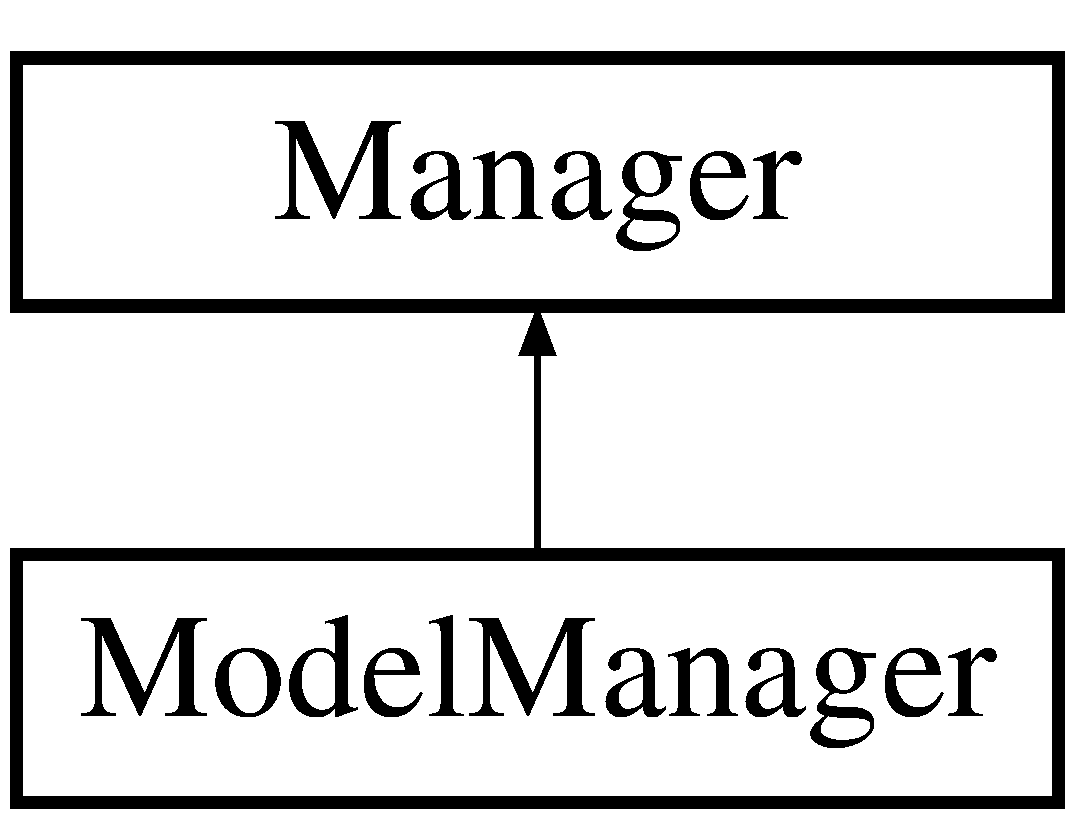
\includegraphics[height=2.000000cm]{class_model_manager}
\end{center}
\end{figure}
\subsection*{Public Member Functions}
\begin{DoxyCompactItemize}
\item 
\hyperlink{class_model_manager_a9b0d22b1baf59c5b566e82fcd8ca424a}{Model\+Manager} ()
\begin{DoxyCompactList}\small\item\em Default constructor. \end{DoxyCompactList}\item 
\hyperlink{class_model_manager_a93f4eea50036cc5453014234aa921c7c}{$\sim$\+Model\+Manager} ()
\begin{DoxyCompactList}\small\item\em Default destructor. \end{DoxyCompactList}\item 
std\+::weak\+\_\+ptr$<$ \hyperlink{class_model}{Model} $>$ \hyperlink{class_model_manager_a2c4b109b70055b540c47ca202d2accf8}{load\+Model} (\hyperlink{class_context}{Context} $\ast$context, const std\+::string \&id, const std\+::string \&path)
\begin{DoxyCompactList}\small\item\em Load a model from an O\+BJ file at a given path. \end{DoxyCompactList}\item 
void \hyperlink{class_model_manager_a38d48d14d9e917b233bb115ebac2809b}{add\+Model} (const std\+::string \&id, std\+::shared\+\_\+ptr$<$ \hyperlink{class_model}{Model} $>$ model)
\begin{DoxyCompactList}\small\item\em Add a model to the manager. \end{DoxyCompactList}\item 
std\+::weak\+\_\+ptr$<$ \hyperlink{class_model}{Model} $>$ \hyperlink{class_model_manager_ae85e1de097acb0c11ba546af7f86d60a}{get\+Model} (const std\+::string \&id)
\begin{DoxyCompactList}\small\item\em Access a model from inside the manager. \end{DoxyCompactList}\item 
void \hyperlink{class_model_manager_af18912c600422fbdaddf25e169006dac}{remove\+Model} (const std\+::string \&id)
\begin{DoxyCompactList}\small\item\em Remove a model from the manager (and kill if applicable) \end{DoxyCompactList}\item 
void \hyperlink{class_model_manager_a7e0bb3438ed9c054ab76297ae71ac78e}{remove\+All\+Models} ()
\begin{DoxyCompactList}\small\item\em Remove all models from the manager (and kill if applicable) \end{DoxyCompactList}\end{DoxyCompactItemize}
\subsection*{Private Attributes}
\begin{DoxyCompactItemize}
\item 
std\+::map$<$ std\+::string, std\+::shared\+\_\+ptr$<$ \hyperlink{class_model}{Model} $>$ $>$ \hyperlink{class_model_manager_a3ce5116dfeff87737e315a4df49bde54}{m\+\_\+\+Models}
\end{DoxyCompactItemize}


\subsection{Detailed Description}
A manager class for handling and passing around model data. 

\begin{DoxyAuthor}{Author}
Hayley Hatton 
\end{DoxyAuthor}
\begin{DoxyDate}{Date}
13/03/2016 
\end{DoxyDate}
\begin{DoxySeeAlso}{See also}
\hyperlink{class_manager}{Manager} 
\end{DoxySeeAlso}


Definition at line 14 of file Model\+Manager.\+h.



\subsection{Constructor \& Destructor Documentation}
\index{Model\+Manager@{Model\+Manager}!Model\+Manager@{Model\+Manager}}
\index{Model\+Manager@{Model\+Manager}!Model\+Manager@{Model\+Manager}}
\subsubsection[{\texorpdfstring{Model\+Manager()}{ModelManager()}}]{\setlength{\rightskip}{0pt plus 5cm}Model\+Manager\+::\+Model\+Manager (
\begin{DoxyParamCaption}
{}
\end{DoxyParamCaption}
)}\hypertarget{class_model_manager_a9b0d22b1baf59c5b566e82fcd8ca424a}{}\label{class_model_manager_a9b0d22b1baf59c5b566e82fcd8ca424a}


Default constructor. 



Definition at line 4 of file Model\+Manager.\+cpp.

\index{Model\+Manager@{Model\+Manager}!````~Model\+Manager@{$\sim$\+Model\+Manager}}
\index{````~Model\+Manager@{$\sim$\+Model\+Manager}!Model\+Manager@{Model\+Manager}}
\subsubsection[{\texorpdfstring{$\sim$\+Model\+Manager()}{~ModelManager()}}]{\setlength{\rightskip}{0pt plus 5cm}Model\+Manager\+::$\sim$\+Model\+Manager (
\begin{DoxyParamCaption}
{}
\end{DoxyParamCaption}
)}\hypertarget{class_model_manager_a93f4eea50036cc5453014234aa921c7c}{}\label{class_model_manager_a93f4eea50036cc5453014234aa921c7c}


Default destructor. 



Definition at line 8 of file Model\+Manager.\+cpp.



\subsection{Member Function Documentation}
\index{Model\+Manager@{Model\+Manager}!add\+Model@{add\+Model}}
\index{add\+Model@{add\+Model}!Model\+Manager@{Model\+Manager}}
\subsubsection[{\texorpdfstring{add\+Model(const std\+::string \&id, std\+::shared\+\_\+ptr$<$ Model $>$ model)}{addModel(const std::string &id, std::shared_ptr< Model > model)}}]{\setlength{\rightskip}{0pt plus 5cm}void Model\+Manager\+::add\+Model (
\begin{DoxyParamCaption}
\item[{const std\+::string \&}]{id, }
\item[{std\+::shared\+\_\+ptr$<$ {\bf Model} $>$}]{model}
\end{DoxyParamCaption}
)}\hypertarget{class_model_manager_a38d48d14d9e917b233bb115ebac2809b}{}\label{class_model_manager_a38d48d14d9e917b233bb115ebac2809b}


Add a model to the manager. 


\begin{DoxyParams}{Parameters}
{\em id} & Identifying name of the model \\
\hline
{\em model} & Smart pointer to the model data class \\
\hline
\end{DoxyParams}


Definition at line 31 of file Model\+Manager.\+cpp.



References m\+\_\+\+Models.

\index{Model\+Manager@{Model\+Manager}!get\+Model@{get\+Model}}
\index{get\+Model@{get\+Model}!Model\+Manager@{Model\+Manager}}
\subsubsection[{\texorpdfstring{get\+Model(const std\+::string \&id)}{getModel(const std::string &id)}}]{\setlength{\rightskip}{0pt plus 5cm}std\+::weak\+\_\+ptr$<$ {\bf Model} $>$ Model\+Manager\+::get\+Model (
\begin{DoxyParamCaption}
\item[{const std\+::string \&}]{id}
\end{DoxyParamCaption}
)}\hypertarget{class_model_manager_ae85e1de097acb0c11ba546af7f86d60a}{}\label{class_model_manager_ae85e1de097acb0c11ba546af7f86d60a}


Access a model from inside the manager. 


\begin{DoxyParams}{Parameters}
{\em id} & Identifying name of the model \\
\hline
\end{DoxyParams}
\begin{DoxyReturn}{Returns}
Weak-\/managed pointer to the model data class; empty if not found 
\end{DoxyReturn}


Definition at line 38 of file Model\+Manager.\+cpp.



References m\+\_\+\+Models.

\index{Model\+Manager@{Model\+Manager}!load\+Model@{load\+Model}}
\index{load\+Model@{load\+Model}!Model\+Manager@{Model\+Manager}}
\subsubsection[{\texorpdfstring{load\+Model(\+Context $\ast$context, const std\+::string \&id, const std\+::string \&path)}{loadModel(Context *context, const std::string &id, const std::string &path)}}]{\setlength{\rightskip}{0pt plus 5cm}std\+::weak\+\_\+ptr$<$ {\bf Model} $>$ Model\+Manager\+::load\+Model (
\begin{DoxyParamCaption}
\item[{{\bf Context} $\ast$}]{context, }
\item[{const std\+::string \&}]{id, }
\item[{const std\+::string \&}]{path}
\end{DoxyParamCaption}
)}\hypertarget{class_model_manager_a2c4b109b70055b540c47ca202d2accf8}{}\label{class_model_manager_a2c4b109b70055b540c47ca202d2accf8}


Load a model from an O\+BJ file at a given path. 


\begin{DoxyParams}{Parameters}
{\em context} & Graphics context \\
\hline
{\em id} & Identifying name of the model \\
\hline
{\em path} & Path to the O\+BJ file \\
\hline
\end{DoxyParams}
\begin{DoxyReturn}{Returns}
Weak-\/managed pointer to the model data class 
\end{DoxyReturn}
\begin{DoxySeeAlso}{See also}
\hyperlink{class_model_loader}{Model\+Loader} 
\end{DoxySeeAlso}


Definition at line 13 of file Model\+Manager.\+cpp.



References m\+\_\+\+Models.

\index{Model\+Manager@{Model\+Manager}!remove\+All\+Models@{remove\+All\+Models}}
\index{remove\+All\+Models@{remove\+All\+Models}!Model\+Manager@{Model\+Manager}}
\subsubsection[{\texorpdfstring{remove\+All\+Models()}{removeAllModels()}}]{\setlength{\rightskip}{0pt plus 5cm}void Model\+Manager\+::remove\+All\+Models (
\begin{DoxyParamCaption}
{}
\end{DoxyParamCaption}
)}\hypertarget{class_model_manager_a7e0bb3438ed9c054ab76297ae71ac78e}{}\label{class_model_manager_a7e0bb3438ed9c054ab76297ae71ac78e}


Remove all models from the manager (and kill if applicable) 



Definition at line 52 of file Model\+Manager.\+cpp.



References m\+\_\+\+Models.

\index{Model\+Manager@{Model\+Manager}!remove\+Model@{remove\+Model}}
\index{remove\+Model@{remove\+Model}!Model\+Manager@{Model\+Manager}}
\subsubsection[{\texorpdfstring{remove\+Model(const std\+::string \&id)}{removeModel(const std::string &id)}}]{\setlength{\rightskip}{0pt plus 5cm}void Model\+Manager\+::remove\+Model (
\begin{DoxyParamCaption}
\item[{const std\+::string \&}]{id}
\end{DoxyParamCaption}
)}\hypertarget{class_model_manager_af18912c600422fbdaddf25e169006dac}{}\label{class_model_manager_af18912c600422fbdaddf25e169006dac}


Remove a model from the manager (and kill if applicable) 


\begin{DoxyParams}{Parameters}
{\em id} & Identifying name of the model \\
\hline
\end{DoxyParams}


Definition at line 47 of file Model\+Manager.\+cpp.



References m\+\_\+\+Models.



\subsection{Member Data Documentation}
\index{Model\+Manager@{Model\+Manager}!m\+\_\+\+Models@{m\+\_\+\+Models}}
\index{m\+\_\+\+Models@{m\+\_\+\+Models}!Model\+Manager@{Model\+Manager}}
\subsubsection[{\texorpdfstring{m\+\_\+\+Models}{m_Models}}]{\setlength{\rightskip}{0pt plus 5cm}std\+::map$<$std\+::string, std\+::shared\+\_\+ptr$<${\bf Model}$>$ $>$ Model\+Manager\+::m\+\_\+\+Models\hspace{0.3cm}{\ttfamily [private]}}\hypertarget{class_model_manager_a3ce5116dfeff87737e315a4df49bde54}{}\label{class_model_manager_a3ce5116dfeff87737e315a4df49bde54}


Definition at line 65 of file Model\+Manager.\+h.



Referenced by add\+Model(), get\+Model(), load\+Model(), remove\+All\+Models(), and remove\+Model().



The documentation for this class was generated from the following files\+:\begin{DoxyCompactItemize}
\item 
Lunar\+Drift/engine/managers/\hyperlink{_model_manager_8h}{Model\+Manager.\+h}\item 
Lunar\+Drift/engine/managers/\hyperlink{_model_manager_8cpp}{Model\+Manager.\+cpp}\end{DoxyCompactItemize}

\hypertarget{class_open_g_l_exception}{}\section{Open\+G\+L\+Exception Class Reference}
\label{class_open_g_l_exception}\index{Open\+G\+L\+Exception@{Open\+G\+L\+Exception}}


Exception raised whenever an Open\+GL subsystem fails.  




{\ttfamily \#include $<$Open\+G\+L\+Exception.\+h$>$}

Inheritance diagram for Open\+G\+L\+Exception\+:\begin{figure}[H]
\begin{center}
\leavevmode
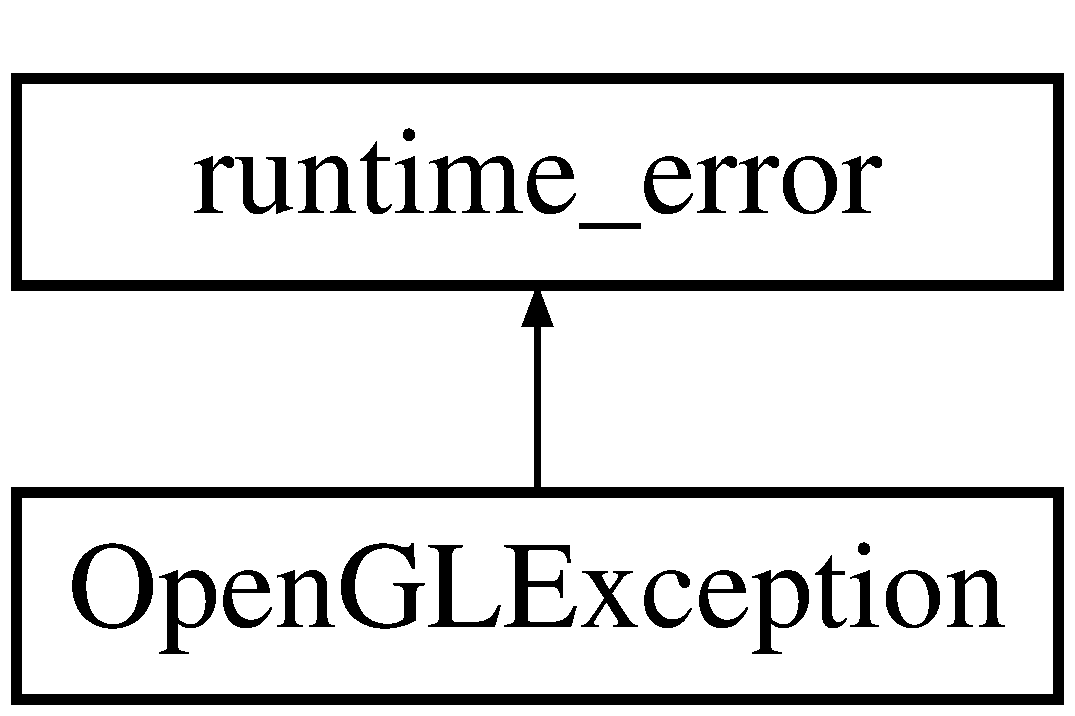
\includegraphics[height=2.000000cm]{class_open_g_l_exception}
\end{center}
\end{figure}
\subsection*{Public Member Functions}
\begin{DoxyCompactItemize}
\item 
\hyperlink{class_open_g_l_exception_ad11d7e03c2a4ca5b8a01f8c2f85a3c4a}{Open\+G\+L\+Exception} (const std\+::string \&report, G\+Lenum gl\+Error\+Code)
\begin{DoxyCompactList}\small\item\em Default constructor. \end{DoxyCompactList}\item 
const std\+::string \& \hyperlink{class_open_g_l_exception_a23e4708e8368cd7bbe93a43a604c523f}{get\+Report} () const 
\item 
G\+Lenum \hyperlink{class_open_g_l_exception_af56f3ea850dd3d2c5e295c6c5a9ed7cb}{get\+G\+L\+Error\+Code} () const 
\item 
const std\+::string \hyperlink{class_open_g_l_exception_aa2465505504557e4a2b30f78830df389}{gl\+Error\+Code\+To\+String} (G\+Lenum gl\+Error\+Code) const 
\end{DoxyCompactItemize}
\subsection*{Private Attributes}
\begin{DoxyCompactItemize}
\item 
const std\+::string \hyperlink{class_open_g_l_exception_a0f9575c625fdb797da165443277e1a54}{m\+\_\+\+Report}
\item 
const G\+Lenum \hyperlink{class_open_g_l_exception_ae92e43b987e00c0a6ea264fbbb1371cd}{m\+\_\+\+G\+L\+Error\+Code}
\end{DoxyCompactItemize}


\subsection{Detailed Description}
Exception raised whenever an Open\+GL subsystem fails. 

\begin{DoxyAuthor}{Author}
Hayley Hatton 
\end{DoxyAuthor}
\begin{DoxyDate}{Date}
20/02/2016 
\end{DoxyDate}


Definition at line 13 of file Open\+G\+L\+Exception.\+h.



\subsection{Constructor \& Destructor Documentation}
\index{Open\+G\+L\+Exception@{Open\+G\+L\+Exception}!Open\+G\+L\+Exception@{Open\+G\+L\+Exception}}
\index{Open\+G\+L\+Exception@{Open\+G\+L\+Exception}!Open\+G\+L\+Exception@{Open\+G\+L\+Exception}}
\subsubsection[{\texorpdfstring{Open\+G\+L\+Exception(const std\+::string \&report, G\+Lenum gl\+Error\+Code)}{OpenGLException(const std::string &report, GLenum glErrorCode)}}]{\setlength{\rightskip}{0pt plus 5cm}Open\+G\+L\+Exception\+::\+Open\+G\+L\+Exception (
\begin{DoxyParamCaption}
\item[{const std\+::string \&}]{report, }
\item[{G\+Lenum}]{gl\+Error\+Code}
\end{DoxyParamCaption}
)}\hypertarget{class_open_g_l_exception_ad11d7e03c2a4ca5b8a01f8c2f85a3c4a}{}\label{class_open_g_l_exception_ad11d7e03c2a4ca5b8a01f8c2f85a3c4a}


Default constructor. 


\begin{DoxyParams}{Parameters}
{\em report} & Error string \\
\hline
{\em gl\+Error\+Code} & Open\+GL A\+PI error code \\
\hline
\end{DoxyParams}


Definition at line 4 of file Open\+G\+L\+Exception.\+cpp.



\subsection{Member Function Documentation}
\index{Open\+G\+L\+Exception@{Open\+G\+L\+Exception}!get\+G\+L\+Error\+Code@{get\+G\+L\+Error\+Code}}
\index{get\+G\+L\+Error\+Code@{get\+G\+L\+Error\+Code}!Open\+G\+L\+Exception@{Open\+G\+L\+Exception}}
\subsubsection[{\texorpdfstring{get\+G\+L\+Error\+Code() const }{getGLErrorCode() const }}]{\setlength{\rightskip}{0pt plus 5cm}G\+Lenum Open\+G\+L\+Exception\+::get\+G\+L\+Error\+Code (
\begin{DoxyParamCaption}
{}
\end{DoxyParamCaption}
) const\hspace{0.3cm}{\ttfamily [inline]}}\hypertarget{class_open_g_l_exception_af56f3ea850dd3d2c5e295c6c5a9ed7cb}{}\label{class_open_g_l_exception_af56f3ea850dd3d2c5e295c6c5a9ed7cb}


Definition at line 28 of file Open\+G\+L\+Exception.\+h.



References gl\+Error\+Code\+To\+String(), and m\+\_\+\+G\+L\+Error\+Code.



Referenced by Window\+P\+C\+::rendering\+Thread(), and Win\+Main().

\index{Open\+G\+L\+Exception@{Open\+G\+L\+Exception}!get\+Report@{get\+Report}}
\index{get\+Report@{get\+Report}!Open\+G\+L\+Exception@{Open\+G\+L\+Exception}}
\subsubsection[{\texorpdfstring{get\+Report() const }{getReport() const }}]{\setlength{\rightskip}{0pt plus 5cm}const std\+::string\& Open\+G\+L\+Exception\+::get\+Report (
\begin{DoxyParamCaption}
{}
\end{DoxyParamCaption}
) const\hspace{0.3cm}{\ttfamily [inline]}}\hypertarget{class_open_g_l_exception_a23e4708e8368cd7bbe93a43a604c523f}{}\label{class_open_g_l_exception_a23e4708e8368cd7bbe93a43a604c523f}


Definition at line 26 of file Open\+G\+L\+Exception.\+h.



References m\+\_\+\+Report.



Referenced by Window\+P\+C\+::rendering\+Thread(), and Win\+Main().

\index{Open\+G\+L\+Exception@{Open\+G\+L\+Exception}!gl\+Error\+Code\+To\+String@{gl\+Error\+Code\+To\+String}}
\index{gl\+Error\+Code\+To\+String@{gl\+Error\+Code\+To\+String}!Open\+G\+L\+Exception@{Open\+G\+L\+Exception}}
\subsubsection[{\texorpdfstring{gl\+Error\+Code\+To\+String(\+G\+Lenum gl\+Error\+Code) const }{glErrorCodeToString(GLenum glErrorCode) const }}]{\setlength{\rightskip}{0pt plus 5cm}const std\+::string Open\+G\+L\+Exception\+::gl\+Error\+Code\+To\+String (
\begin{DoxyParamCaption}
\item[{G\+Lenum}]{gl\+Error\+Code}
\end{DoxyParamCaption}
) const}\hypertarget{class_open_g_l_exception_aa2465505504557e4a2b30f78830df389}{}\label{class_open_g_l_exception_aa2465505504557e4a2b30f78830df389}


Definition at line 24 of file Open\+G\+L\+Exception.\+cpp.



References to\+\_\+string().



Referenced by get\+G\+L\+Error\+Code(), Window\+P\+C\+::rendering\+Thread(), and Win\+Main().



\subsection{Member Data Documentation}
\index{Open\+G\+L\+Exception@{Open\+G\+L\+Exception}!m\+\_\+\+G\+L\+Error\+Code@{m\+\_\+\+G\+L\+Error\+Code}}
\index{m\+\_\+\+G\+L\+Error\+Code@{m\+\_\+\+G\+L\+Error\+Code}!Open\+G\+L\+Exception@{Open\+G\+L\+Exception}}
\subsubsection[{\texorpdfstring{m\+\_\+\+G\+L\+Error\+Code}{m_GLErrorCode}}]{\setlength{\rightskip}{0pt plus 5cm}const G\+Lenum Open\+G\+L\+Exception\+::m\+\_\+\+G\+L\+Error\+Code\hspace{0.3cm}{\ttfamily [private]}}\hypertarget{class_open_g_l_exception_ae92e43b987e00c0a6ea264fbbb1371cd}{}\label{class_open_g_l_exception_ae92e43b987e00c0a6ea264fbbb1371cd}


Definition at line 34 of file Open\+G\+L\+Exception.\+h.



Referenced by get\+G\+L\+Error\+Code().

\index{Open\+G\+L\+Exception@{Open\+G\+L\+Exception}!m\+\_\+\+Report@{m\+\_\+\+Report}}
\index{m\+\_\+\+Report@{m\+\_\+\+Report}!Open\+G\+L\+Exception@{Open\+G\+L\+Exception}}
\subsubsection[{\texorpdfstring{m\+\_\+\+Report}{m_Report}}]{\setlength{\rightskip}{0pt plus 5cm}const std\+::string Open\+G\+L\+Exception\+::m\+\_\+\+Report\hspace{0.3cm}{\ttfamily [private]}}\hypertarget{class_open_g_l_exception_a0f9575c625fdb797da165443277e1a54}{}\label{class_open_g_l_exception_a0f9575c625fdb797da165443277e1a54}


Definition at line 33 of file Open\+G\+L\+Exception.\+h.



Referenced by get\+Report().



The documentation for this class was generated from the following files\+:\begin{DoxyCompactItemize}
\item 
Lunar\+Drift/engine/exceptions/\hyperlink{_open_g_l_exception_8h}{Open\+G\+L\+Exception.\+h}\item 
Lunar\+Drift/engine/exceptions/\hyperlink{_open_g_l_exception_8cpp}{Open\+G\+L\+Exception.\+cpp}\end{DoxyCompactItemize}

\hypertarget{class_program}{}\section{Program Class Reference}
\label{class_program}\index{Program@{Program}}


Top-\/level program entry point class.  




{\ttfamily \#include $<$Program.\+h$>$}

Inheritance diagram for Program\+:\begin{figure}[H]
\begin{center}
\leavevmode
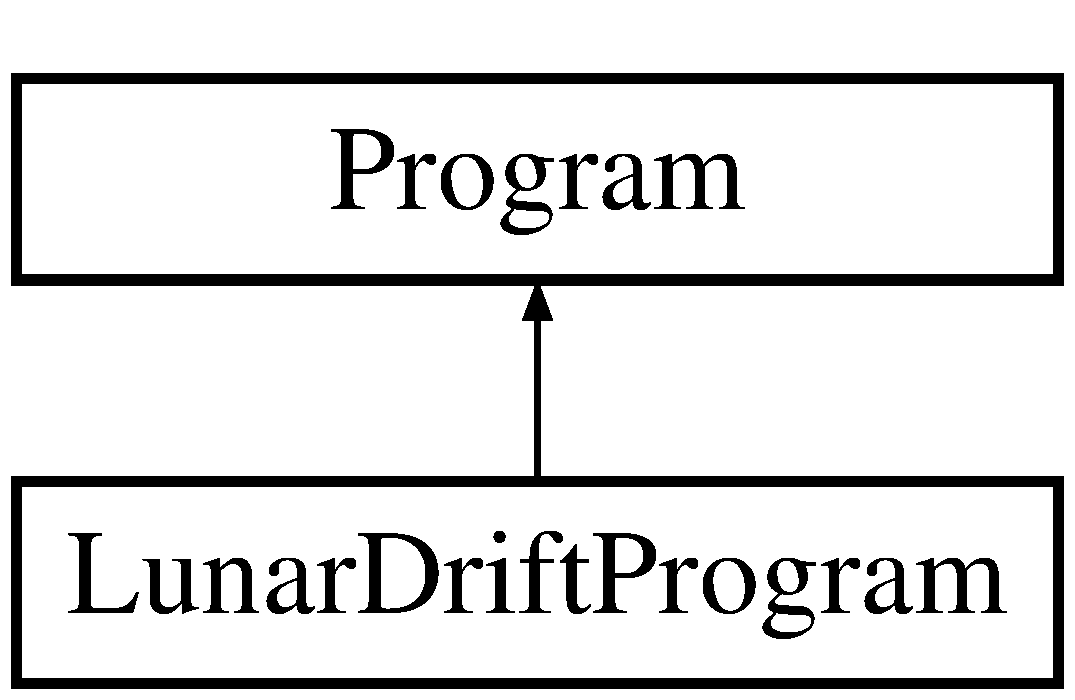
\includegraphics[height=2.000000cm]{class_program}
\end{center}
\end{figure}
\subsection*{Public Member Functions}
\begin{DoxyCompactItemize}
\item 
\hyperlink{class_program_a051939fcd1eef21aa8a77f200b15c4ab}{Program} (const std\+::string \&name, \hyperlink{class_context}{Context} $\ast$context)
\begin{DoxyCompactList}\small\item\em Object-\/oriented entry point to the program. \end{DoxyCompactList}\item 
virtual \hyperlink{class_program_a986aef1c50e1d338a3315a47ba6df549}{$\sim$\+Program} ()
\begin{DoxyCompactList}\small\item\em Default destructor. \end{DoxyCompactList}\item 
const std\+::string \& \hyperlink{class_program_a826e23457377f1c8c834f2d2808ceca8}{get\+Name} () const 
\begin{DoxyCompactList}\small\item\em Access the name of the program. \end{DoxyCompactList}\item 
virtual void \hyperlink{class_program_a975de71413195823c525955cfd5f2ca7}{step} (double dt)
\begin{DoxyCompactList}\small\item\em Called on the stepping of the simulation state. \end{DoxyCompactList}\item 
virtual void \hyperlink{class_program_a3b02a58d4c366e280759bc8bbdd4b50d}{frame} (\hyperlink{class_context}{Context} $\ast$context)
\begin{DoxyCompactList}\small\item\em Called on the rendering of a frame. \end{DoxyCompactList}\end{DoxyCompactItemize}
\subsection*{Protected Member Functions}
\begin{DoxyCompactItemize}
\item 
void \hyperlink{class_program_ad76eb179a68360571ea857f5ce7ce126}{set\+Renderer} (\hyperlink{class_context}{Context} $\ast$context, std\+::shared\+\_\+ptr$<$ \hyperlink{class_renderer}{Renderer} $>$ renderer)
\begin{DoxyCompactList}\small\item\em Set the active renderer to render the scenes with. \end{DoxyCompactList}\item 
virtual std\+::shared\+\_\+ptr$<$ \hyperlink{class_renderer}{Renderer} $>$ \hyperlink{class_program_a016ef26d3d6b6aeffd3b4e74dfde033e}{get\+Renderer} (\hyperlink{class_context}{Context} $\ast$context) const  =0
\begin{DoxyCompactList}\small\item\em Retrieve a new renderer for a given stereo mode from the subclass. \end{DoxyCompactList}\item 
void \hyperlink{class_program_a0bfe1a80dedb4bfaddfc6ab364c4e62a}{set\+Active\+Scene} (std\+::shared\+\_\+ptr$<$ \hyperlink{class_scene}{Scene} $>$ scene)
\begin{DoxyCompactList}\small\item\em Set the active scene to manage and render. \end{DoxyCompactList}\end{DoxyCompactItemize}
\subsection*{Private Attributes}
\begin{DoxyCompactItemize}
\item 
const std\+::string \hyperlink{class_program_a69d3c5c15cf8167d59e4d8c25e915063}{m\+\_\+\+Name}
\begin{DoxyCompactList}\small\item\em Name of the program. \end{DoxyCompactList}\item 
std\+::shared\+\_\+ptr$<$ \hyperlink{class_renderer}{Renderer} $>$ \hyperlink{class_program_a0aaeb79e919a8009806510e5dca10f50}{m\+\_\+\+Renderer}
\begin{DoxyCompactList}\small\item\em Active renderer. \end{DoxyCompactList}\item 
std\+::shared\+\_\+ptr$<$ \hyperlink{class_scene}{Scene} $>$ \hyperlink{class_program_a261d54bdb11938ff460af06232f8580f}{m\+\_\+\+Active\+Scene}
\begin{DoxyCompactList}\small\item\em Active scene. \end{DoxyCompactList}\end{DoxyCompactItemize}


\subsection{Detailed Description}
Top-\/level program entry point class. 

\begin{DoxyAuthor}{Author}
Hayley Hatton 
\end{DoxyAuthor}
\begin{DoxyDate}{Date}
20/02/2016 
\end{DoxyDate}


Definition at line 14 of file Program.\+h.



\subsection{Constructor \& Destructor Documentation}
\index{Program@{Program}!Program@{Program}}
\index{Program@{Program}!Program@{Program}}
\subsubsection[{\texorpdfstring{Program(const std\+::string \&name, Context $\ast$context)}{Program(const std::string &name, Context *context)}}]{\setlength{\rightskip}{0pt plus 5cm}Program\+::\+Program (
\begin{DoxyParamCaption}
\item[{const std\+::string \&}]{name, }
\item[{{\bf Context} $\ast$}]{context}
\end{DoxyParamCaption}
)}\hypertarget{class_program_a051939fcd1eef21aa8a77f200b15c4ab}{}\label{class_program_a051939fcd1eef21aa8a77f200b15c4ab}


Object-\/oriented entry point to the program. 


\begin{DoxyParams}{Parameters}
{\em name} & String name of the program \\
\hline
{\em context} & Graphics context \\
\hline
\end{DoxyParams}


Definition at line 5 of file Program.\+cpp.

\index{Program@{Program}!````~Program@{$\sim$\+Program}}
\index{````~Program@{$\sim$\+Program}!Program@{Program}}
\subsubsection[{\texorpdfstring{$\sim$\+Program()}{~Program()}}]{\setlength{\rightskip}{0pt plus 5cm}Program\+::$\sim$\+Program (
\begin{DoxyParamCaption}
{}
\end{DoxyParamCaption}
)\hspace{0.3cm}{\ttfamily [virtual]}}\hypertarget{class_program_a986aef1c50e1d338a3315a47ba6df549}{}\label{class_program_a986aef1c50e1d338a3315a47ba6df549}


Default destructor. 



Definition at line 12 of file Program.\+cpp.



\subsection{Member Function Documentation}
\index{Program@{Program}!frame@{frame}}
\index{frame@{frame}!Program@{Program}}
\subsubsection[{\texorpdfstring{frame(\+Context $\ast$context)}{frame(Context *context)}}]{\setlength{\rightskip}{0pt plus 5cm}void Program\+::frame (
\begin{DoxyParamCaption}
\item[{{\bf Context} $\ast$}]{context}
\end{DoxyParamCaption}
)\hspace{0.3cm}{\ttfamily [virtual]}}\hypertarget{class_program_a3b02a58d4c366e280759bc8bbdd4b50d}{}\label{class_program_a3b02a58d4c366e280759bc8bbdd4b50d}


Called on the rendering of a frame. 


\begin{DoxyParams}{Parameters}
{\em context} & Graphical context \\
\hline
\end{DoxyParams}


Reimplemented in \hyperlink{class_lunar_drift_program_a5db9835b135348644bc940cd7c2870be}{Lunar\+Drift\+Program}.



Definition at line 23 of file Program.\+cpp.



References get\+Renderer(), m\+\_\+\+Active\+Scene, m\+\_\+\+Renderer, and set\+Renderer().



Referenced by Lunar\+Drift\+Program\+::frame(), get\+Name(), and Window\+P\+C\+::rendering\+Thread().

\index{Program@{Program}!get\+Name@{get\+Name}}
\index{get\+Name@{get\+Name}!Program@{Program}}
\subsubsection[{\texorpdfstring{get\+Name() const }{getName() const }}]{\setlength{\rightskip}{0pt plus 5cm}const std\+::string\& Program\+::get\+Name (
\begin{DoxyParamCaption}
{}
\end{DoxyParamCaption}
) const\hspace{0.3cm}{\ttfamily [inline]}}\hypertarget{class_program_a826e23457377f1c8c834f2d2808ceca8}{}\label{class_program_a826e23457377f1c8c834f2d2808ceca8}


Access the name of the program. 

\begin{DoxyReturn}{Returns}
Reference to name. Do not keep the reference; copy instead 
\end{DoxyReturn}


Definition at line 32 of file Program.\+h.



References frame(), get\+Renderer(), m\+\_\+\+Name, set\+Active\+Scene(), set\+Renderer(), and step().

\index{Program@{Program}!get\+Renderer@{get\+Renderer}}
\index{get\+Renderer@{get\+Renderer}!Program@{Program}}
\subsubsection[{\texorpdfstring{get\+Renderer(\+Context $\ast$context) const  =0}{getRenderer(Context *context) const  =0}}]{\setlength{\rightskip}{0pt plus 5cm}virtual std\+::shared\+\_\+ptr$<${\bf Renderer}$>$ Program\+::get\+Renderer (
\begin{DoxyParamCaption}
\item[{{\bf Context} $\ast$}]{context}
\end{DoxyParamCaption}
) const\hspace{0.3cm}{\ttfamily [protected]}, {\ttfamily [pure virtual]}}\hypertarget{class_program_a016ef26d3d6b6aeffd3b4e74dfde033e}{}\label{class_program_a016ef26d3d6b6aeffd3b4e74dfde033e}


Retrieve a new renderer for a given stereo mode from the subclass. 


\begin{DoxyParams}{Parameters}
{\em context} & Graphics context \\
\hline
{\em mode} & Type of stereo renderer requested by the system \\
\hline
\end{DoxyParams}
\begin{DoxyReturn}{Returns}
Smart pointer to the new appropriate renderer 
\end{DoxyReturn}


Implemented in \hyperlink{class_lunar_drift_program_a19fa2f0a909951f9e5cfdd7b5392be85}{Lunar\+Drift\+Program}.



Referenced by frame(), and get\+Name().

\index{Program@{Program}!set\+Active\+Scene@{set\+Active\+Scene}}
\index{set\+Active\+Scene@{set\+Active\+Scene}!Program@{Program}}
\subsubsection[{\texorpdfstring{set\+Active\+Scene(std\+::shared\+\_\+ptr$<$ Scene $>$ scene)}{setActiveScene(std::shared_ptr< Scene > scene)}}]{\setlength{\rightskip}{0pt plus 5cm}void Program\+::set\+Active\+Scene (
\begin{DoxyParamCaption}
\item[{std\+::shared\+\_\+ptr$<$ {\bf Scene} $>$}]{scene}
\end{DoxyParamCaption}
)\hspace{0.3cm}{\ttfamily [protected]}}\hypertarget{class_program_a0bfe1a80dedb4bfaddfc6ab364c4e62a}{}\label{class_program_a0bfe1a80dedb4bfaddfc6ab364c4e62a}


Set the active scene to manage and render. 


\begin{DoxyParams}{Parameters}
{\em scene} & Active scene \\
\hline
\end{DoxyParams}


Definition at line 43 of file Program.\+cpp.



References m\+\_\+\+Active\+Scene.



Referenced by get\+Name(), and Lunar\+Drift\+Program\+::\+Lunar\+Drift\+Program().

\index{Program@{Program}!set\+Renderer@{set\+Renderer}}
\index{set\+Renderer@{set\+Renderer}!Program@{Program}}
\subsubsection[{\texorpdfstring{set\+Renderer(\+Context $\ast$context, std\+::shared\+\_\+ptr$<$ Renderer $>$ renderer)}{setRenderer(Context *context, std::shared_ptr< Renderer > renderer)}}]{\setlength{\rightskip}{0pt plus 5cm}void Program\+::set\+Renderer (
\begin{DoxyParamCaption}
\item[{{\bf Context} $\ast$}]{context, }
\item[{std\+::shared\+\_\+ptr$<$ {\bf Renderer} $>$}]{renderer}
\end{DoxyParamCaption}
)\hspace{0.3cm}{\ttfamily [protected]}}\hypertarget{class_program_ad76eb179a68360571ea857f5ce7ce126}{}\label{class_program_ad76eb179a68360571ea857f5ce7ce126}


Set the active renderer to render the scenes with. 


\begin{DoxyParams}{Parameters}
{\em context} & Graphics context \\
\hline
{\em renderer} & \hyperlink{class_renderer}{Renderer} to draw with \\
\hline
\end{DoxyParams}


Definition at line 36 of file Program.\+cpp.



References m\+\_\+\+Renderer.



Referenced by frame(), and get\+Name().

\index{Program@{Program}!step@{step}}
\index{step@{step}!Program@{Program}}
\subsubsection[{\texorpdfstring{step(double dt)}{step(double dt)}}]{\setlength{\rightskip}{0pt plus 5cm}void Program\+::step (
\begin{DoxyParamCaption}
\item[{double}]{dt}
\end{DoxyParamCaption}
)\hspace{0.3cm}{\ttfamily [virtual]}}\hypertarget{class_program_a975de71413195823c525955cfd5f2ca7}{}\label{class_program_a975de71413195823c525955cfd5f2ca7}


Called on the stepping of the simulation state. 


\begin{DoxyParams}{Parameters}
{\em dt} & Delta time, in seconds \\
\hline
\end{DoxyParams}


Reimplemented in \hyperlink{class_lunar_drift_program_a3467aea42888a3eae28d587c90e5b1ff}{Lunar\+Drift\+Program}.



Definition at line 17 of file Program.\+cpp.



References m\+\_\+\+Active\+Scene.



Referenced by get\+Name(), Window\+P\+C\+::simulation\+Thread(), and Lunar\+Drift\+Program\+::step().



\subsection{Member Data Documentation}
\index{Program@{Program}!m\+\_\+\+Active\+Scene@{m\+\_\+\+Active\+Scene}}
\index{m\+\_\+\+Active\+Scene@{m\+\_\+\+Active\+Scene}!Program@{Program}}
\subsubsection[{\texorpdfstring{m\+\_\+\+Active\+Scene}{m_ActiveScene}}]{\setlength{\rightskip}{0pt plus 5cm}std\+::shared\+\_\+ptr$<${\bf Scene}$>$ Program\+::m\+\_\+\+Active\+Scene\hspace{0.3cm}{\ttfamily [private]}}\hypertarget{class_program_a261d54bdb11938ff460af06232f8580f}{}\label{class_program_a261d54bdb11938ff460af06232f8580f}


Active scene. 



Definition at line 72 of file Program.\+h.



Referenced by frame(), set\+Active\+Scene(), and step().

\index{Program@{Program}!m\+\_\+\+Name@{m\+\_\+\+Name}}
\index{m\+\_\+\+Name@{m\+\_\+\+Name}!Program@{Program}}
\subsubsection[{\texorpdfstring{m\+\_\+\+Name}{m_Name}}]{\setlength{\rightskip}{0pt plus 5cm}const std\+::string Program\+::m\+\_\+\+Name\hspace{0.3cm}{\ttfamily [private]}}\hypertarget{class_program_a69d3c5c15cf8167d59e4d8c25e915063}{}\label{class_program_a69d3c5c15cf8167d59e4d8c25e915063}


Name of the program. 



Definition at line 70 of file Program.\+h.



Referenced by get\+Name().

\index{Program@{Program}!m\+\_\+\+Renderer@{m\+\_\+\+Renderer}}
\index{m\+\_\+\+Renderer@{m\+\_\+\+Renderer}!Program@{Program}}
\subsubsection[{\texorpdfstring{m\+\_\+\+Renderer}{m_Renderer}}]{\setlength{\rightskip}{0pt plus 5cm}std\+::shared\+\_\+ptr$<${\bf Renderer}$>$ Program\+::m\+\_\+\+Renderer\hspace{0.3cm}{\ttfamily [private]}}\hypertarget{class_program_a0aaeb79e919a8009806510e5dca10f50}{}\label{class_program_a0aaeb79e919a8009806510e5dca10f50}


Active renderer. 



Definition at line 71 of file Program.\+h.



Referenced by frame(), and set\+Renderer().



The documentation for this class was generated from the following files\+:\begin{DoxyCompactItemize}
\item 
Lunar\+Drift/engine/\hyperlink{_program_8h}{Program.\+h}\item 
Lunar\+Drift/engine/\hyperlink{_program_8cpp}{Program.\+cpp}\end{DoxyCompactItemize}

\hypertarget{class_renderer}{}\section{Renderer Class Reference}
\label{class_renderer}\index{Renderer@{Renderer}}


Abstract renderer for drawing scenes with a given graphics context.  




{\ttfamily \#include $<$Renderer.\+h$>$}

Inheritance diagram for Renderer\+:\begin{figure}[H]
\begin{center}
\leavevmode
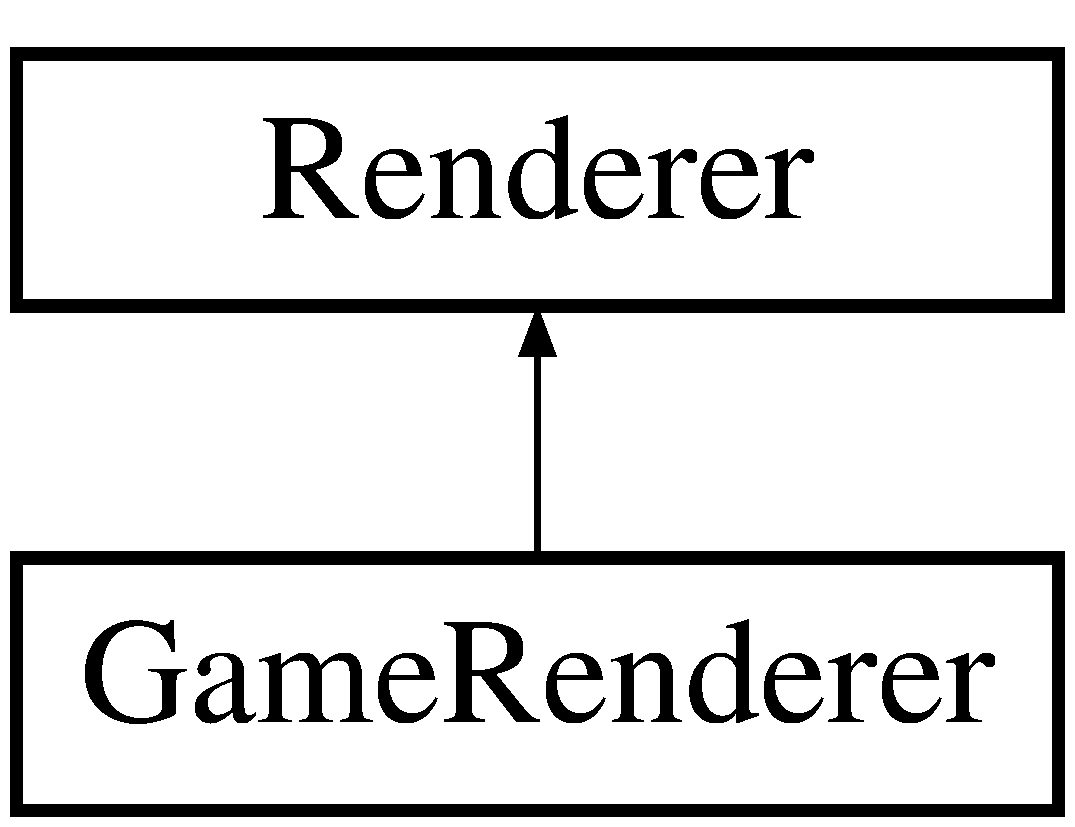
\includegraphics[height=2.000000cm]{class_renderer}
\end{center}
\end{figure}
\subsection*{Public Member Functions}
\begin{DoxyCompactItemize}
\item 
\hyperlink{class_renderer_a21f9183202b351da1d4c9d20fbf6a7db}{Renderer} (\hyperlink{class_context}{Context} $\ast$context, G\+Lsizei width, G\+Lsizei height)
\begin{DoxyCompactList}\small\item\em Default constructor. \end{DoxyCompactList}\item 
virtual \hyperlink{class_renderer_afeee408862d5bd6255a6882d47e6d5cd}{$\sim$\+Renderer} ()
\begin{DoxyCompactList}\small\item\em Default destructor. \end{DoxyCompactList}\item 
void \hyperlink{class_renderer_a3a63289ee0d3b291b43f8c99d445140a}{get\+Dimensions} (G\+Lsizei $\ast$width, G\+Lsizei $\ast$height) const 
\begin{DoxyCompactList}\small\item\em Access the dimensions of the full rendering context. \end{DoxyCompactList}\item 
virtual void \hyperlink{class_renderer_a73b37f476662d7dcbc8f02b1ee8b7e66}{pre\+Frame} (\hyperlink{class_context}{Context} $\ast$context, std\+::shared\+\_\+ptr$<$ \hyperlink{class_scene}{Scene} $>$ scene)
\begin{DoxyCompactList}\small\item\em Called before the frame is drawn; useful for setting up the frame. \end{DoxyCompactList}\item 
virtual void \hyperlink{class_renderer_ac6bd2531e087c99d44298100a1db7631}{frame} (\hyperlink{class_context}{Context} $\ast$context, std\+::shared\+\_\+ptr$<$ \hyperlink{class_scene}{Scene} $>$ scene)
\begin{DoxyCompactList}\small\item\em Called to draw the frame. \end{DoxyCompactList}\item 
virtual void \hyperlink{class_renderer_affc664549db066d9219579f8fd5cd657}{post\+Frame} (\hyperlink{class_context}{Context} $\ast$context, std\+::shared\+\_\+ptr$<$ \hyperlink{class_scene}{Scene} $>$ scene)
\begin{DoxyCompactList}\small\item\em Called after the frame is drawn; useful for posting the frame. \end{DoxyCompactList}\item 
void \hyperlink{class_renderer_a8dd7e25ac4d1930cfa6a4533ed80557d}{set\+Clear\+Color} (const glm\+::vec4 \&color)
\item 
void \hyperlink{class_renderer_a8c77522a011a90dfc30929b8d9d3cf1e}{resize} (G\+Lsizei width, G\+Lsizei height)
\begin{DoxyCompactList}\small\item\em Resize the renderer. \end{DoxyCompactList}\end{DoxyCompactItemize}
\subsection*{Protected Member Functions}
\begin{DoxyCompactItemize}
\item 
void \hyperlink{class_renderer_a9efd7bd25d602491adbd823b0b7d311c}{set\+Size} (\hyperlink{class_context}{Context} $\ast$context, std\+::shared\+\_\+ptr$<$ \hyperlink{class_scene}{Scene} $>$ scene)
\begin{DoxyCompactList}\small\item\em Update the viewport and echo changes to the scene. \end{DoxyCompactList}\item 
virtual std\+::shared\+\_\+ptr$<$ \hyperlink{class_shader_manager}{Shader\+Manager} $>$ \hyperlink{class_renderer_a18aeed0fc26835778f23a2ff7406446b}{load\+Standard\+Shaders} (\hyperlink{class_context}{Context} $\ast$context)=0
\begin{DoxyCompactList}\small\item\em Create and return a shader manager containing the standard shaders. \end{DoxyCompactList}\item 
void \hyperlink{class_renderer_a14aeed9016bcd66be47862ed3749d7dc}{load} (\hyperlink{class_context}{Context} $\ast$context)
\begin{DoxyCompactList}\small\item\em Load the renderer. \end{DoxyCompactList}\item 
void \hyperlink{class_renderer_aa9ca4685f6e82578dec01db053ceef8d}{update\+Shader\+States} (\hyperlink{class_context}{Context} $\ast$context, std\+::shared\+\_\+ptr$<$ \hyperlink{class_scene}{Scene} $>$ scene, std\+::shared\+\_\+ptr$<$ \hyperlink{class_shader_manager}{Shader\+Manager} $>$ shaders)
\begin{DoxyCompactList}\small\item\em Update the shader states of all the shaders in a shader manager. \end{DoxyCompactList}\item 
void \hyperlink{class_renderer_af3ebba8a1565bca7359944b72f56d719}{draw\+Scene} (\hyperlink{class_context}{Context} $\ast$context, std\+::shared\+\_\+ptr$<$ \hyperlink{class_scene}{Scene} $>$ scene, std\+::shared\+\_\+ptr$<$ \hyperlink{class_shader_manager}{Shader\+Manager} $>$ shaders)
\begin{DoxyCompactList}\small\item\em Draw a scene using a given shader manager. \end{DoxyCompactList}\end{DoxyCompactItemize}
\subsection*{Private Attributes}
\begin{DoxyCompactItemize}
\item 
G\+Lsizei \hyperlink{class_renderer_ad70df586fdb171b32e3c5b4a31a5104b}{m\+\_\+\+Width\+Px}
\item 
G\+Lsizei \hyperlink{class_renderer_a6a89127b886568aceb1ad94f1c2584e9}{m\+\_\+\+Height\+Px}
\item 
bool \hyperlink{class_renderer_a7b739cc1443319e00d0c675a27c7e17b}{m\+\_\+\+Resized}
\item 
glm\+::vec4 \hyperlink{class_renderer_a9d5ab43b148e3d440e43cf0d7325dec7}{m\+\_\+\+Clear\+Color}
\item 
std\+::shared\+\_\+ptr$<$ \hyperlink{class_shader_manager}{Shader\+Manager} $>$ \hyperlink{class_renderer_a45692735f3f2562d55f8d51c4bc5fd1c}{m\+\_\+\+Standard\+Shaders}
\end{DoxyCompactItemize}


\subsection{Detailed Description}
Abstract renderer for drawing scenes with a given graphics context. 

\begin{DoxyAuthor}{Author}
Hayley Hatton 
\end{DoxyAuthor}
\begin{DoxyDate}{Date}
20/02/2016 
\end{DoxyDate}


Definition at line 13 of file Renderer.\+h.



\subsection{Constructor \& Destructor Documentation}
\index{Renderer@{Renderer}!Renderer@{Renderer}}
\index{Renderer@{Renderer}!Renderer@{Renderer}}
\subsubsection[{\texorpdfstring{Renderer(\+Context $\ast$context, G\+Lsizei width, G\+Lsizei height)}{Renderer(Context *context, GLsizei width, GLsizei height)}}]{\setlength{\rightskip}{0pt plus 5cm}Renderer\+::\+Renderer (
\begin{DoxyParamCaption}
\item[{{\bf Context} $\ast$}]{context, }
\item[{G\+Lsizei}]{width, }
\item[{G\+Lsizei}]{height}
\end{DoxyParamCaption}
)}\hypertarget{class_renderer_a21f9183202b351da1d4c9d20fbf6a7db}{}\label{class_renderer_a21f9183202b351da1d4c9d20fbf6a7db}


Default constructor. 


\begin{DoxyParams}{Parameters}
{\em context} & Graphics context \\
\hline
{\em width} & Width of context in pixels \\
\hline
{\em height} & Height of context in pixels \\
\hline
\end{DoxyParams}


Definition at line 4 of file Renderer.\+cpp.



References f.

\index{Renderer@{Renderer}!````~Renderer@{$\sim$\+Renderer}}
\index{````~Renderer@{$\sim$\+Renderer}!Renderer@{Renderer}}
\subsubsection[{\texorpdfstring{$\sim$\+Renderer()}{~Renderer()}}]{\setlength{\rightskip}{0pt plus 5cm}Renderer\+::$\sim$\+Renderer (
\begin{DoxyParamCaption}
{}
\end{DoxyParamCaption}
)\hspace{0.3cm}{\ttfamily [virtual]}}\hypertarget{class_renderer_afeee408862d5bd6255a6882d47e6d5cd}{}\label{class_renderer_afeee408862d5bd6255a6882d47e6d5cd}


Default destructor. 



Definition at line 12 of file Renderer.\+cpp.



\subsection{Member Function Documentation}
\index{Renderer@{Renderer}!draw\+Scene@{draw\+Scene}}
\index{draw\+Scene@{draw\+Scene}!Renderer@{Renderer}}
\subsubsection[{\texorpdfstring{draw\+Scene(\+Context $\ast$context, std\+::shared\+\_\+ptr$<$ Scene $>$ scene, std\+::shared\+\_\+ptr$<$ Shader\+Manager $>$ shaders)}{drawScene(Context *context, std::shared_ptr< Scene > scene, std::shared_ptr< ShaderManager > shaders)}}]{\setlength{\rightskip}{0pt plus 5cm}void Renderer\+::draw\+Scene (
\begin{DoxyParamCaption}
\item[{{\bf Context} $\ast$}]{context, }
\item[{std\+::shared\+\_\+ptr$<$ {\bf Scene} $>$}]{scene, }
\item[{std\+::shared\+\_\+ptr$<$ {\bf Shader\+Manager} $>$}]{shaders}
\end{DoxyParamCaption}
)\hspace{0.3cm}{\ttfamily [protected]}}\hypertarget{class_renderer_af3ebba8a1565bca7359944b72f56d719}{}\label{class_renderer_af3ebba8a1565bca7359944b72f56d719}


Draw a scene using a given shader manager. 


\begin{DoxyParams}{Parameters}
{\em context} & Graphics context \\
\hline
{\em scene} & Smart pointer to the scene instance to draw \\
\hline
{\em shaders} & Smart pointer to the shader manager to draw scene with \\
\hline
\end{DoxyParams}


Definition at line 68 of file Renderer.\+cpp.



Referenced by frame(), and set\+Clear\+Color().

\index{Renderer@{Renderer}!frame@{frame}}
\index{frame@{frame}!Renderer@{Renderer}}
\subsubsection[{\texorpdfstring{frame(\+Context $\ast$context, std\+::shared\+\_\+ptr$<$ Scene $>$ scene)}{frame(Context *context, std::shared_ptr< Scene > scene)}}]{\setlength{\rightskip}{0pt plus 5cm}void Renderer\+::frame (
\begin{DoxyParamCaption}
\item[{{\bf Context} $\ast$}]{context, }
\item[{std\+::shared\+\_\+ptr$<$ {\bf Scene} $>$}]{scene}
\end{DoxyParamCaption}
)\hspace{0.3cm}{\ttfamily [virtual]}}\hypertarget{class_renderer_ac6bd2531e087c99d44298100a1db7631}{}\label{class_renderer_ac6bd2531e087c99d44298100a1db7631}


Called to draw the frame. 


\begin{DoxyParams}{Parameters}
{\em context} & Graphics context \\
\hline
{\em scene} & Smart pointer to the scene to render \\
\hline
\end{DoxyParams}


Definition at line 84 of file Renderer.\+cpp.



References draw\+Scene(), m\+\_\+\+Resized, m\+\_\+\+Standard\+Shaders, set\+Size(), and update\+Shader\+States().

\index{Renderer@{Renderer}!get\+Dimensions@{get\+Dimensions}}
\index{get\+Dimensions@{get\+Dimensions}!Renderer@{Renderer}}
\subsubsection[{\texorpdfstring{get\+Dimensions(\+G\+Lsizei $\ast$width, G\+Lsizei $\ast$height) const }{getDimensions(GLsizei *width, GLsizei *height) const }}]{\setlength{\rightskip}{0pt plus 5cm}void Renderer\+::get\+Dimensions (
\begin{DoxyParamCaption}
\item[{G\+Lsizei $\ast$}]{width, }
\item[{G\+Lsizei $\ast$}]{height}
\end{DoxyParamCaption}
) const}\hypertarget{class_renderer_a3a63289ee0d3b291b43f8c99d445140a}{}\label{class_renderer_a3a63289ee0d3b291b43f8c99d445140a}


Access the dimensions of the full rendering context. 


\begin{DoxyParams}{Parameters}
{\em width} & Pointer to store width in pixels \\
\hline
{\em height} & Pointer to store height in pixels \\
\hline
\end{DoxyParams}


Definition at line 18 of file Renderer.\+cpp.



References m\+\_\+\+Height\+Px, and m\+\_\+\+Width\+Px.



Referenced by set\+Size().

\index{Renderer@{Renderer}!load@{load}}
\index{load@{load}!Renderer@{Renderer}}
\subsubsection[{\texorpdfstring{load(\+Context $\ast$context)}{load(Context *context)}}]{\setlength{\rightskip}{0pt plus 5cm}void Renderer\+::load (
\begin{DoxyParamCaption}
\item[{{\bf Context} $\ast$}]{context}
\end{DoxyParamCaption}
)\hspace{0.3cm}{\ttfamily [protected]}}\hypertarget{class_renderer_a14aeed9016bcd66be47862ed3749d7dc}{}\label{class_renderer_a14aeed9016bcd66be47862ed3749d7dc}


Load the renderer. 


\begin{DoxyParams}{Parameters}
{\em context} & Graphics context \\
\hline
\end{DoxyParams}


Definition at line 101 of file Renderer.\+cpp.



References load\+Standard\+Shaders(), and m\+\_\+\+Standard\+Shaders.



Referenced by Game\+Renderer\+::\+Game\+Renderer(), and set\+Clear\+Color().

\index{Renderer@{Renderer}!load\+Standard\+Shaders@{load\+Standard\+Shaders}}
\index{load\+Standard\+Shaders@{load\+Standard\+Shaders}!Renderer@{Renderer}}
\subsubsection[{\texorpdfstring{load\+Standard\+Shaders(\+Context $\ast$context)=0}{loadStandardShaders(Context *context)=0}}]{\setlength{\rightskip}{0pt plus 5cm}virtual std\+::shared\+\_\+ptr$<${\bf Shader\+Manager}$>$ Renderer\+::load\+Standard\+Shaders (
\begin{DoxyParamCaption}
\item[{{\bf Context} $\ast$}]{context}
\end{DoxyParamCaption}
)\hspace{0.3cm}{\ttfamily [protected]}, {\ttfamily [pure virtual]}}\hypertarget{class_renderer_a18aeed0fc26835778f23a2ff7406446b}{}\label{class_renderer_a18aeed0fc26835778f23a2ff7406446b}


Create and return a shader manager containing the standard shaders. 

\begin{DoxyReturn}{Returns}
Managed pointer of a default shader manager 
\end{DoxyReturn}


Implemented in \hyperlink{class_game_renderer_ac01f6745a9dd800dfe4c5fb12d46bc38}{Game\+Renderer}.



Referenced by load(), and set\+Clear\+Color().

\index{Renderer@{Renderer}!post\+Frame@{post\+Frame}}
\index{post\+Frame@{post\+Frame}!Renderer@{Renderer}}
\subsubsection[{\texorpdfstring{post\+Frame(\+Context $\ast$context, std\+::shared\+\_\+ptr$<$ Scene $>$ scene)}{postFrame(Context *context, std::shared_ptr< Scene > scene)}}]{\setlength{\rightskip}{0pt plus 5cm}void Renderer\+::post\+Frame (
\begin{DoxyParamCaption}
\item[{{\bf Context} $\ast$}]{context, }
\item[{std\+::shared\+\_\+ptr$<$ {\bf Scene} $>$}]{scene}
\end{DoxyParamCaption}
)\hspace{0.3cm}{\ttfamily [virtual]}}\hypertarget{class_renderer_affc664549db066d9219579f8fd5cd657}{}\label{class_renderer_affc664549db066d9219579f8fd5cd657}


Called after the frame is drawn; useful for posting the frame. 


\begin{DoxyParams}{Parameters}
{\em context} & Graphics context \\
\hline
{\em scene} & Smart pointer to the scene to render \\
\hline
\end{DoxyParams}


Definition at line 96 of file Renderer.\+cpp.

\index{Renderer@{Renderer}!pre\+Frame@{pre\+Frame}}
\index{pre\+Frame@{pre\+Frame}!Renderer@{Renderer}}
\subsubsection[{\texorpdfstring{pre\+Frame(\+Context $\ast$context, std\+::shared\+\_\+ptr$<$ Scene $>$ scene)}{preFrame(Context *context, std::shared_ptr< Scene > scene)}}]{\setlength{\rightskip}{0pt plus 5cm}void Renderer\+::pre\+Frame (
\begin{DoxyParamCaption}
\item[{{\bf Context} $\ast$}]{context, }
\item[{std\+::shared\+\_\+ptr$<$ {\bf Scene} $>$}]{scene}
\end{DoxyParamCaption}
)\hspace{0.3cm}{\ttfamily [virtual]}}\hypertarget{class_renderer_a73b37f476662d7dcbc8f02b1ee8b7e66}{}\label{class_renderer_a73b37f476662d7dcbc8f02b1ee8b7e66}


Called before the frame is drawn; useful for setting up the frame. 


\begin{DoxyParams}{Parameters}
{\em context} & Graphics context \\
\hline
{\em scene} & Smart pointer to the scene to render \\
\hline
\end{DoxyParams}


Definition at line 46 of file Renderer.\+cpp.



References m\+\_\+\+Clear\+Color.

\index{Renderer@{Renderer}!resize@{resize}}
\index{resize@{resize}!Renderer@{Renderer}}
\subsubsection[{\texorpdfstring{resize(\+G\+Lsizei width, G\+Lsizei height)}{resize(GLsizei width, GLsizei height)}}]{\setlength{\rightskip}{0pt plus 5cm}void Renderer\+::resize (
\begin{DoxyParamCaption}
\item[{G\+Lsizei}]{width, }
\item[{G\+Lsizei}]{height}
\end{DoxyParamCaption}
)}\hypertarget{class_renderer_a8c77522a011a90dfc30929b8d9d3cf1e}{}\label{class_renderer_a8c77522a011a90dfc30929b8d9d3cf1e}


Resize the renderer. 


\begin{DoxyParams}{Parameters}
{\em width} & New width of GL context in pixels \\
\hline
{\em height} & New height of GL context in pixels \\
\hline
\end{DoxyParams}


Definition at line 24 of file Renderer.\+cpp.



References m\+\_\+\+Height\+Px, m\+\_\+\+Resized, and m\+\_\+\+Width\+Px.



Referenced by set\+Clear\+Color().

\index{Renderer@{Renderer}!set\+Clear\+Color@{set\+Clear\+Color}}
\index{set\+Clear\+Color@{set\+Clear\+Color}!Renderer@{Renderer}}
\subsubsection[{\texorpdfstring{set\+Clear\+Color(const glm\+::vec4 \&color)}{setClearColor(const glm::vec4 &color)}}]{\setlength{\rightskip}{0pt plus 5cm}void Renderer\+::set\+Clear\+Color (
\begin{DoxyParamCaption}
\item[{const glm\+::vec4 \&}]{color}
\end{DoxyParamCaption}
)\hspace{0.3cm}{\ttfamily [inline]}}\hypertarget{class_renderer_a8dd7e25ac4d1930cfa6a4533ed80557d}{}\label{class_renderer_a8dd7e25ac4d1930cfa6a4533ed80557d}


Definition at line 56 of file Renderer.\+h.



References draw\+Scene(), load(), load\+Standard\+Shaders(), m\+\_\+\+Clear\+Color, resize(), set\+Size(), and update\+Shader\+States().



Referenced by Game\+Renderer\+::\+Game\+Renderer().

\index{Renderer@{Renderer}!set\+Size@{set\+Size}}
\index{set\+Size@{set\+Size}!Renderer@{Renderer}}
\subsubsection[{\texorpdfstring{set\+Size(\+Context $\ast$context, std\+::shared\+\_\+ptr$<$ Scene $>$ scene)}{setSize(Context *context, std::shared_ptr< Scene > scene)}}]{\setlength{\rightskip}{0pt plus 5cm}void Renderer\+::set\+Size (
\begin{DoxyParamCaption}
\item[{{\bf Context} $\ast$}]{context, }
\item[{std\+::shared\+\_\+ptr$<$ {\bf Scene} $>$}]{scene}
\end{DoxyParamCaption}
)\hspace{0.3cm}{\ttfamily [protected]}}\hypertarget{class_renderer_a9efd7bd25d602491adbd823b0b7d311c}{}\label{class_renderer_a9efd7bd25d602491adbd823b0b7d311c}


Update the viewport and echo changes to the scene. 


\begin{DoxyParams}{Parameters}
{\em context} & Graphics context \\
\hline
{\em scene} & Smart pointer to the scene to resize \\
\hline
\end{DoxyParams}


Definition at line 31 of file Renderer.\+cpp.



References get\+Dimensions(), h, m\+\_\+\+Resized, and w.



Referenced by frame(), and set\+Clear\+Color().

\index{Renderer@{Renderer}!update\+Shader\+States@{update\+Shader\+States}}
\index{update\+Shader\+States@{update\+Shader\+States}!Renderer@{Renderer}}
\subsubsection[{\texorpdfstring{update\+Shader\+States(\+Context $\ast$context, std\+::shared\+\_\+ptr$<$ Scene $>$ scene, std\+::shared\+\_\+ptr$<$ Shader\+Manager $>$ shaders)}{updateShaderStates(Context *context, std::shared_ptr< Scene > scene, std::shared_ptr< ShaderManager > shaders)}}]{\setlength{\rightskip}{0pt plus 5cm}void Renderer\+::update\+Shader\+States (
\begin{DoxyParamCaption}
\item[{{\bf Context} $\ast$}]{context, }
\item[{std\+::shared\+\_\+ptr$<$ {\bf Scene} $>$}]{scene, }
\item[{std\+::shared\+\_\+ptr$<$ {\bf Shader\+Manager} $>$}]{shaders}
\end{DoxyParamCaption}
)\hspace{0.3cm}{\ttfamily [protected]}}\hypertarget{class_renderer_aa9ca4685f6e82578dec01db053ceef8d}{}\label{class_renderer_aa9ca4685f6e82578dec01db053ceef8d}


Update the shader states of all the shaders in a shader manager. 


\begin{DoxyParams}{Parameters}
{\em context} & Graphics context \\
\hline
{\em scene} & Smart pointer to the scene instance to use \\
\hline
{\em shaders} & Smart pointer to the shader manager to update states with \\
\hline
\end{DoxyParams}


Definition at line 55 of file Renderer.\+cpp.



Referenced by frame(), and set\+Clear\+Color().



\subsection{Member Data Documentation}
\index{Renderer@{Renderer}!m\+\_\+\+Clear\+Color@{m\+\_\+\+Clear\+Color}}
\index{m\+\_\+\+Clear\+Color@{m\+\_\+\+Clear\+Color}!Renderer@{Renderer}}
\subsubsection[{\texorpdfstring{m\+\_\+\+Clear\+Color}{m_ClearColor}}]{\setlength{\rightskip}{0pt plus 5cm}glm\+::vec4 Renderer\+::m\+\_\+\+Clear\+Color\hspace{0.3cm}{\ttfamily [private]}}\hypertarget{class_renderer_a9d5ab43b148e3d440e43cf0d7325dec7}{}\label{class_renderer_a9d5ab43b148e3d440e43cf0d7325dec7}


Definition at line 111 of file Renderer.\+h.



Referenced by pre\+Frame(), and set\+Clear\+Color().

\index{Renderer@{Renderer}!m\+\_\+\+Height\+Px@{m\+\_\+\+Height\+Px}}
\index{m\+\_\+\+Height\+Px@{m\+\_\+\+Height\+Px}!Renderer@{Renderer}}
\subsubsection[{\texorpdfstring{m\+\_\+\+Height\+Px}{m_HeightPx}}]{\setlength{\rightskip}{0pt plus 5cm}G\+Lsizei Renderer\+::m\+\_\+\+Height\+Px\hspace{0.3cm}{\ttfamily [private]}}\hypertarget{class_renderer_a6a89127b886568aceb1ad94f1c2584e9}{}\label{class_renderer_a6a89127b886568aceb1ad94f1c2584e9}


Definition at line 109 of file Renderer.\+h.



Referenced by get\+Dimensions(), and resize().

\index{Renderer@{Renderer}!m\+\_\+\+Resized@{m\+\_\+\+Resized}}
\index{m\+\_\+\+Resized@{m\+\_\+\+Resized}!Renderer@{Renderer}}
\subsubsection[{\texorpdfstring{m\+\_\+\+Resized}{m_Resized}}]{\setlength{\rightskip}{0pt plus 5cm}bool Renderer\+::m\+\_\+\+Resized\hspace{0.3cm}{\ttfamily [private]}}\hypertarget{class_renderer_a7b739cc1443319e00d0c675a27c7e17b}{}\label{class_renderer_a7b739cc1443319e00d0c675a27c7e17b}


Definition at line 110 of file Renderer.\+h.



Referenced by frame(), resize(), and set\+Size().

\index{Renderer@{Renderer}!m\+\_\+\+Standard\+Shaders@{m\+\_\+\+Standard\+Shaders}}
\index{m\+\_\+\+Standard\+Shaders@{m\+\_\+\+Standard\+Shaders}!Renderer@{Renderer}}
\subsubsection[{\texorpdfstring{m\+\_\+\+Standard\+Shaders}{m_StandardShaders}}]{\setlength{\rightskip}{0pt plus 5cm}std\+::shared\+\_\+ptr$<${\bf Shader\+Manager}$>$ Renderer\+::m\+\_\+\+Standard\+Shaders\hspace{0.3cm}{\ttfamily [private]}}\hypertarget{class_renderer_a45692735f3f2562d55f8d51c4bc5fd1c}{}\label{class_renderer_a45692735f3f2562d55f8d51c4bc5fd1c}


Definition at line 112 of file Renderer.\+h.



Referenced by frame(), and load().

\index{Renderer@{Renderer}!m\+\_\+\+Width\+Px@{m\+\_\+\+Width\+Px}}
\index{m\+\_\+\+Width\+Px@{m\+\_\+\+Width\+Px}!Renderer@{Renderer}}
\subsubsection[{\texorpdfstring{m\+\_\+\+Width\+Px}{m_WidthPx}}]{\setlength{\rightskip}{0pt plus 5cm}G\+Lsizei Renderer\+::m\+\_\+\+Width\+Px\hspace{0.3cm}{\ttfamily [private]}}\hypertarget{class_renderer_ad70df586fdb171b32e3c5b4a31a5104b}{}\label{class_renderer_ad70df586fdb171b32e3c5b4a31a5104b}


Definition at line 109 of file Renderer.\+h.



Referenced by get\+Dimensions(), and resize().



The documentation for this class was generated from the following files\+:\begin{DoxyCompactItemize}
\item 
Lunar\+Drift/engine/graphics/renderers/\hyperlink{_renderer_8h}{Renderer.\+h}\item 
Lunar\+Drift/engine/graphics/renderers/\hyperlink{_renderer_8cpp}{Renderer.\+cpp}\end{DoxyCompactItemize}

\hypertarget{class_scene}{}\section{Scene Class Reference}
\label{class_scene}\index{Scene@{Scene}}


\hyperlink{class_scene}{Scene} container for managing and drawing 3D environments.  




{\ttfamily \#include $<$Scene.\+h$>$}

Inheritance diagram for Scene\+:\begin{figure}[H]
\begin{center}
\leavevmode
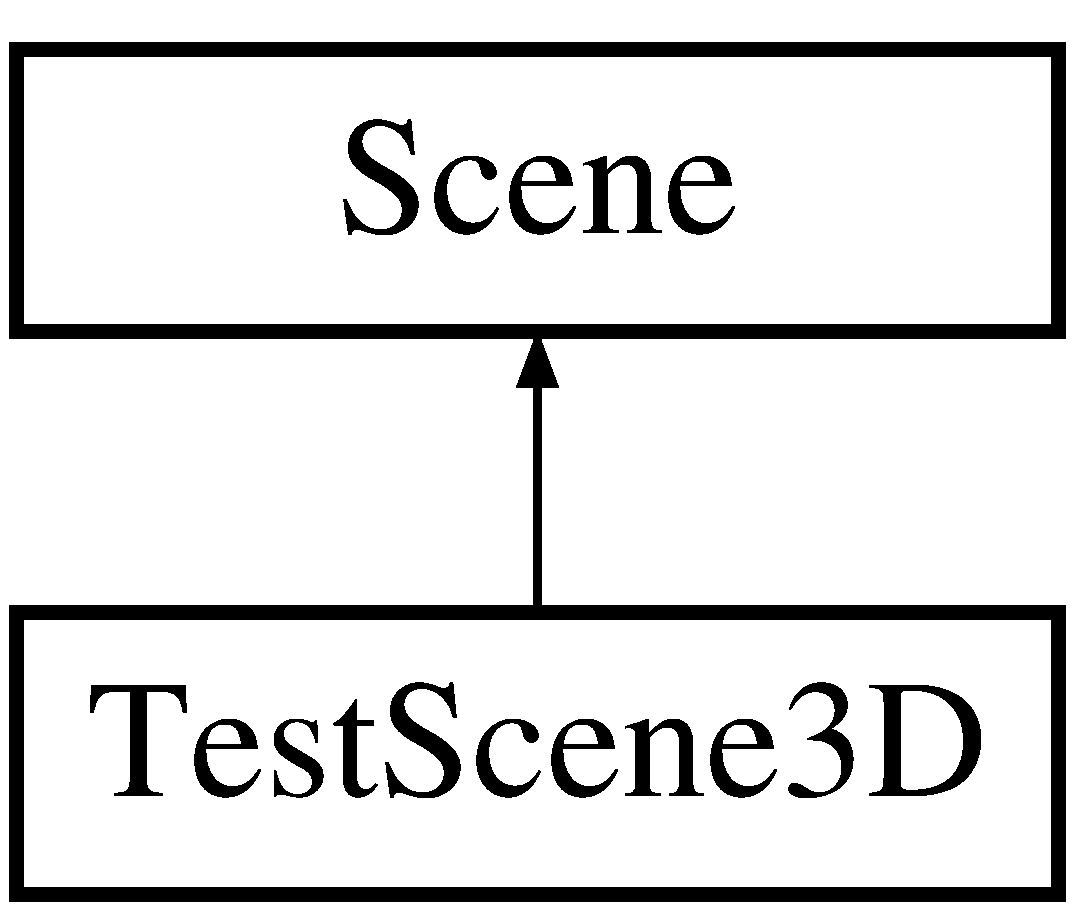
\includegraphics[height=2.000000cm]{class_scene}
\end{center}
\end{figure}
\subsection*{Public Member Functions}
\begin{DoxyCompactItemize}
\item 
\hyperlink{class_scene_ae40169557308d8af0bd57d3f814b1937}{Scene} (\hyperlink{class_context}{Context} $\ast$context)
\begin{DoxyCompactList}\small\item\em Default constructor. \end{DoxyCompactList}\item 
virtual \hyperlink{class_scene_a3b8cec2e32546713915f8c6303c951f1}{$\sim$\+Scene} ()
\begin{DoxyCompactList}\small\item\em Default destructor. \end{DoxyCompactList}\item 
void \hyperlink{class_scene_af0990031fb81e2bec0391a5923911fc3}{get\+Objects} (std\+::list$<$ std\+::shared\+\_\+ptr$<$ \hyperlink{class_scene_object}{Scene\+Object} $>$ $>$ $\ast$objects)
\begin{DoxyCompactList}\small\item\em Retrieve the list of objects in the scene. \end{DoxyCompactList}\item 
const std\+::weak\+\_\+ptr$<$ \hyperlink{class_camera}{Camera} $>$ \hyperlink{class_scene_a314aabca592a5979069563b0845bac2f}{get\+Active\+Camera} () const 
\begin{DoxyCompactList}\small\item\em Access the currently active camera. \end{DoxyCompactList}\item 
virtual void \hyperlink{class_scene_adc13fd7e44ebc5cb6165cb25853420c7}{set\+Size} (G\+Lsizei width, G\+Lsizei height)
\begin{DoxyCompactList}\small\item\em Called to update scene elements with the viewport information. \end{DoxyCompactList}\item 
virtual void \hyperlink{class_scene_aa9597b193a1cd70a276ca2480c01adea}{step} (double dt)
\begin{DoxyCompactList}\small\item\em Step the scene\textquotesingle{}s simulation state. \end{DoxyCompactList}\item 
virtual void \hyperlink{class_scene_a5c993df1c224d17fc3fd618d413e3f87}{predraw} (\hyperlink{class_context}{Context} $\ast$context)
\begin{DoxyCompactList}\small\item\em Called before the renderer draws the scene This allows the scene and its constituent objects to do updates that require a graphics context before the graphical state is drawn. \end{DoxyCompactList}\end{DoxyCompactItemize}
\subsection*{Protected Member Functions}
\begin{DoxyCompactItemize}
\item 
void \hyperlink{class_scene_a4f683b6add0466a6b3fa1357fc27baa3}{add\+Object} (std\+::shared\+\_\+ptr$<$ \hyperlink{class_scene_object}{Scene\+Object} $>$ object)
\begin{DoxyCompactList}\small\item\em Add an object to be managed by the scene. \end{DoxyCompactList}\item 
void \hyperlink{class_scene_a8822b7f23dbd84390024545192779516}{set\+Active\+Camera} (std\+::shared\+\_\+ptr$<$ \hyperlink{class_camera}{Camera} $>$ camera)
\begin{DoxyCompactList}\small\item\em Set the active camera for the scene. \end{DoxyCompactList}\item 
std\+::weak\+\_\+ptr$<$ \hyperlink{class_meta_manager}{Meta\+Manager} $>$ \hyperlink{class_scene_ae0da6dc6945a84f338a4d1907fef0dbc}{get\+Managers} ()
\end{DoxyCompactItemize}
\subsection*{Private Attributes}
\begin{DoxyCompactItemize}
\item 
std\+::shared\+\_\+ptr$<$ \hyperlink{class_meta_manager}{Meta\+Manager} $>$ \hyperlink{class_scene_a40f1ffc374bb488c2ec2599289793316}{m\+\_\+\+Managers}
\item 
std\+::shared\+\_\+ptr$<$ \hyperlink{class_camera}{Camera} $>$ \hyperlink{class_scene_a14eae4c46620f2eac7f3efcc8a8ec0e2}{m\+\_\+\+Active\+Camera}
\begin{DoxyCompactList}\small\item\em \hyperlink{class_camera}{Camera} currently in use. \end{DoxyCompactList}\end{DoxyCompactItemize}


\subsection{Detailed Description}
\hyperlink{class_scene}{Scene} container for managing and drawing 3D environments. 

\begin{DoxyPrecond}{Precondition}
A valid Open\+GL context must be present to the program 
\end{DoxyPrecond}
\begin{DoxyAuthor}{Author}
Hayley Hatton 
\end{DoxyAuthor}
\begin{DoxyDate}{Date}
06/03/2016 
\end{DoxyDate}


Definition at line 15 of file Scene.\+h.



\subsection{Constructor \& Destructor Documentation}
\index{Scene@{Scene}!Scene@{Scene}}
\index{Scene@{Scene}!Scene@{Scene}}
\subsubsection[{\texorpdfstring{Scene(\+Context $\ast$context)}{Scene(Context *context)}}]{\setlength{\rightskip}{0pt plus 5cm}Scene\+::\+Scene (
\begin{DoxyParamCaption}
\item[{{\bf Context} $\ast$}]{context}
\end{DoxyParamCaption}
)}\hypertarget{class_scene_ae40169557308d8af0bd57d3f814b1937}{}\label{class_scene_ae40169557308d8af0bd57d3f814b1937}


Default constructor. 


\begin{DoxyParams}{Parameters}
{\em context} & Graphics context \\
\hline
\end{DoxyParams}


Definition at line 6 of file Scene.\+cpp.



References m\+\_\+\+Managers.

\index{Scene@{Scene}!````~Scene@{$\sim$\+Scene}}
\index{````~Scene@{$\sim$\+Scene}!Scene@{Scene}}
\subsubsection[{\texorpdfstring{$\sim$\+Scene()}{~Scene()}}]{\setlength{\rightskip}{0pt plus 5cm}Scene\+::$\sim$\+Scene (
\begin{DoxyParamCaption}
{}
\end{DoxyParamCaption}
)\hspace{0.3cm}{\ttfamily [virtual]}}\hypertarget{class_scene_a3b8cec2e32546713915f8c6303c951f1}{}\label{class_scene_a3b8cec2e32546713915f8c6303c951f1}


Default destructor. 



Definition at line 14 of file Scene.\+cpp.



\subsection{Member Function Documentation}
\index{Scene@{Scene}!add\+Object@{add\+Object}}
\index{add\+Object@{add\+Object}!Scene@{Scene}}
\subsubsection[{\texorpdfstring{add\+Object(std\+::shared\+\_\+ptr$<$ Scene\+Object $>$ object)}{addObject(std::shared_ptr< SceneObject > object)}}]{\setlength{\rightskip}{0pt plus 5cm}void Scene\+::add\+Object (
\begin{DoxyParamCaption}
\item[{std\+::shared\+\_\+ptr$<$ {\bf Scene\+Object} $>$}]{object}
\end{DoxyParamCaption}
)\hspace{0.3cm}{\ttfamily [protected]}}\hypertarget{class_scene_a4f683b6add0466a6b3fa1357fc27baa3}{}\label{class_scene_a4f683b6add0466a6b3fa1357fc27baa3}


Add an object to be managed by the scene. 


\begin{DoxyParams}{Parameters}
{\em object} & Smart pointer to the scene object \\
\hline
\end{DoxyParams}


Definition at line 28 of file Scene.\+cpp.



References Scene\+Object\+Manager\+::add\+Scene\+Object(), and m\+\_\+\+Managers.



Referenced by Test\+Scene3\+D\+::\+Test\+Scene3\+D().

\index{Scene@{Scene}!get\+Active\+Camera@{get\+Active\+Camera}}
\index{get\+Active\+Camera@{get\+Active\+Camera}!Scene@{Scene}}
\subsubsection[{\texorpdfstring{get\+Active\+Camera() const }{getActiveCamera() const }}]{\setlength{\rightskip}{0pt plus 5cm}const std\+::weak\+\_\+ptr$<$ {\bf Camera} $>$ Scene\+::get\+Active\+Camera (
\begin{DoxyParamCaption}
{}
\end{DoxyParamCaption}
) const}\hypertarget{class_scene_a314aabca592a5979069563b0845bac2f}{}\label{class_scene_a314aabca592a5979069563b0845bac2f}


Access the currently active camera. 

\begin{DoxyReturn}{Returns}
Managed pointer to the currently active camera 
\end{DoxyReturn}


Definition at line 62 of file Scene.\+cpp.



References m\+\_\+\+Active\+Camera.



Referenced by Test\+Scene3\+D\+::set\+Size(), and Test\+Scene3\+D\+::step().

\index{Scene@{Scene}!get\+Managers@{get\+Managers}}
\index{get\+Managers@{get\+Managers}!Scene@{Scene}}
\subsubsection[{\texorpdfstring{get\+Managers()}{getManagers()}}]{\setlength{\rightskip}{0pt plus 5cm}std\+::weak\+\_\+ptr$<${\bf Meta\+Manager}$>$ Scene\+::get\+Managers (
\begin{DoxyParamCaption}
{}
\end{DoxyParamCaption}
)\hspace{0.3cm}{\ttfamily [inline]}, {\ttfamily [protected]}}\hypertarget{class_scene_ae0da6dc6945a84f338a4d1907fef0dbc}{}\label{class_scene_ae0da6dc6945a84f338a4d1907fef0dbc}


Definition at line 75 of file Scene.\+h.



References m\+\_\+\+Managers.



Referenced by Test\+Scene3\+D\+::\+Test\+Scene3\+D().

\index{Scene@{Scene}!get\+Objects@{get\+Objects}}
\index{get\+Objects@{get\+Objects}!Scene@{Scene}}
\subsubsection[{\texorpdfstring{get\+Objects(std\+::list$<$ std\+::shared\+\_\+ptr$<$ Scene\+Object $>$ $>$ $\ast$objects)}{getObjects(std::list< std::shared_ptr< SceneObject > > *objects)}}]{\setlength{\rightskip}{0pt plus 5cm}void Scene\+::get\+Objects (
\begin{DoxyParamCaption}
\item[{std\+::list$<$ std\+::shared\+\_\+ptr$<$ {\bf Scene\+Object} $>$ $>$ $\ast$}]{objects}
\end{DoxyParamCaption}
)}\hypertarget{class_scene_af0990031fb81e2bec0391a5923911fc3}{}\label{class_scene_af0990031fb81e2bec0391a5923911fc3}


Retrieve the list of objects in the scene. 


\begin{DoxyParams}{Parameters}
{\em objects} & Pointer to list to fill with scene objects \\
\hline
\end{DoxyParams}


Definition at line 20 of file Scene.\+cpp.



References Scene\+Object\+Manager\+::get\+Objects(), and m\+\_\+\+Managers.

\index{Scene@{Scene}!predraw@{predraw}}
\index{predraw@{predraw}!Scene@{Scene}}
\subsubsection[{\texorpdfstring{predraw(\+Context $\ast$context)}{predraw(Context *context)}}]{\setlength{\rightskip}{0pt plus 5cm}void Scene\+::predraw (
\begin{DoxyParamCaption}
\item[{{\bf Context} $\ast$}]{context}
\end{DoxyParamCaption}
)\hspace{0.3cm}{\ttfamily [virtual]}}\hypertarget{class_scene_a5c993df1c224d17fc3fd618d413e3f87}{}\label{class_scene_a5c993df1c224d17fc3fd618d413e3f87}


Called before the renderer draws the scene This allows the scene and its constituent objects to do updates that require a graphics context before the graphical state is drawn. 


\begin{DoxyParams}{Parameters}
{\em context} & Graphics context \\
\hline
\end{DoxyParams}


Reimplemented in \hyperlink{class_test_scene3_d_ab87089331bf0fb71d09361624dc1c53e}{Test\+Scene3D}.



Definition at line 49 of file Scene.\+cpp.



References m\+\_\+\+Managers, and Scene\+Object\+Manager\+::predraw().



Referenced by Test\+Scene3\+D\+::predraw().

\index{Scene@{Scene}!set\+Active\+Camera@{set\+Active\+Camera}}
\index{set\+Active\+Camera@{set\+Active\+Camera}!Scene@{Scene}}
\subsubsection[{\texorpdfstring{set\+Active\+Camera(std\+::shared\+\_\+ptr$<$ Camera $>$ camera)}{setActiveCamera(std::shared_ptr< Camera > camera)}}]{\setlength{\rightskip}{0pt plus 5cm}void Scene\+::set\+Active\+Camera (
\begin{DoxyParamCaption}
\item[{std\+::shared\+\_\+ptr$<$ {\bf Camera} $>$}]{camera}
\end{DoxyParamCaption}
)\hspace{0.3cm}{\ttfamily [protected]}}\hypertarget{class_scene_a8822b7f23dbd84390024545192779516}{}\label{class_scene_a8822b7f23dbd84390024545192779516}


Set the active camera for the scene. 


\begin{DoxyParams}{Parameters}
{\em camera} & Smart pointer to the camera to make active \\
\hline
\end{DoxyParams}


Definition at line 57 of file Scene.\+cpp.



References m\+\_\+\+Active\+Camera.



Referenced by Test\+Scene3\+D\+::\+Test\+Scene3\+D().

\index{Scene@{Scene}!set\+Size@{set\+Size}}
\index{set\+Size@{set\+Size}!Scene@{Scene}}
\subsubsection[{\texorpdfstring{set\+Size(\+G\+Lsizei width, G\+Lsizei height)}{setSize(GLsizei width, GLsizei height)}}]{\setlength{\rightskip}{0pt plus 5cm}void Scene\+::set\+Size (
\begin{DoxyParamCaption}
\item[{G\+Lsizei}]{width, }
\item[{G\+Lsizei}]{height}
\end{DoxyParamCaption}
)\hspace{0.3cm}{\ttfamily [virtual]}}\hypertarget{class_scene_adc13fd7e44ebc5cb6165cb25853420c7}{}\label{class_scene_adc13fd7e44ebc5cb6165cb25853420c7}


Called to update scene elements with the viewport information. 


\begin{DoxyParams}{Parameters}
{\em width} & Width of the viewport in pixels \\
\hline
{\em height} & Height of the viewport in pixels \\
\hline
\end{DoxyParams}


Reimplemented in \hyperlink{class_test_scene3_d_ab762c0baa39e323b598f08945d50bb1f}{Test\+Scene3D}.



Definition at line 67 of file Scene.\+cpp.

\index{Scene@{Scene}!step@{step}}
\index{step@{step}!Scene@{Scene}}
\subsubsection[{\texorpdfstring{step(double dt)}{step(double dt)}}]{\setlength{\rightskip}{0pt plus 5cm}void Scene\+::step (
\begin{DoxyParamCaption}
\item[{double}]{dt}
\end{DoxyParamCaption}
)\hspace{0.3cm}{\ttfamily [virtual]}}\hypertarget{class_scene_aa9597b193a1cd70a276ca2480c01adea}{}\label{class_scene_aa9597b193a1cd70a276ca2480c01adea}


Step the scene\textquotesingle{}s simulation state. 


\begin{DoxyParams}{Parameters}
{\em dt} & Delta-\/time since last step call in seconds \\
\hline
\end{DoxyParams}


Reimplemented in \hyperlink{class_test_scene3_d_aebf275cd7c567dca7d8662ff859d2acf}{Test\+Scene3D}.



Definition at line 36 of file Scene.\+cpp.



References Collision\+Manager\+::do\+Collisions(), m\+\_\+\+Managers, and Scene\+Object\+Manager\+::step().



Referenced by Test\+Scene3\+D\+::step().



\subsection{Member Data Documentation}
\index{Scene@{Scene}!m\+\_\+\+Active\+Camera@{m\+\_\+\+Active\+Camera}}
\index{m\+\_\+\+Active\+Camera@{m\+\_\+\+Active\+Camera}!Scene@{Scene}}
\subsubsection[{\texorpdfstring{m\+\_\+\+Active\+Camera}{m_ActiveCamera}}]{\setlength{\rightskip}{0pt plus 5cm}std\+::shared\+\_\+ptr$<${\bf Camera}$>$ Scene\+::m\+\_\+\+Active\+Camera\hspace{0.3cm}{\ttfamily [private]}}\hypertarget{class_scene_a14eae4c46620f2eac7f3efcc8a8ec0e2}{}\label{class_scene_a14eae4c46620f2eac7f3efcc8a8ec0e2}


\hyperlink{class_camera}{Camera} currently in use. 



Definition at line 79 of file Scene.\+h.



Referenced by get\+Active\+Camera(), and set\+Active\+Camera().

\index{Scene@{Scene}!m\+\_\+\+Managers@{m\+\_\+\+Managers}}
\index{m\+\_\+\+Managers@{m\+\_\+\+Managers}!Scene@{Scene}}
\subsubsection[{\texorpdfstring{m\+\_\+\+Managers}{m_Managers}}]{\setlength{\rightskip}{0pt plus 5cm}std\+::shared\+\_\+ptr$<${\bf Meta\+Manager}$>$ Scene\+::m\+\_\+\+Managers\hspace{0.3cm}{\ttfamily [private]}}\hypertarget{class_scene_a40f1ffc374bb488c2ec2599289793316}{}\label{class_scene_a40f1ffc374bb488c2ec2599289793316}


Definition at line 78 of file Scene.\+h.



Referenced by add\+Object(), get\+Managers(), get\+Objects(), predraw(), Scene(), and step().



The documentation for this class was generated from the following files\+:\begin{DoxyCompactItemize}
\item 
Lunar\+Drift/engine/containers/\hyperlink{_scene_8h}{Scene.\+h}\item 
Lunar\+Drift/engine/containers/\hyperlink{_scene_8cpp}{Scene.\+cpp}\end{DoxyCompactItemize}

\hypertarget{class_scene_object}{}\section{Scene\+Object Class Reference}
\label{class_scene_object}\index{Scene\+Object@{Scene\+Object}}


Abstract class for encapsulating self-\/management of scene entities.  




{\ttfamily \#include $<$Scene\+Object.\+h$>$}

Inheritance diagram for Scene\+Object\+:\begin{figure}[H]
\begin{center}
\leavevmode
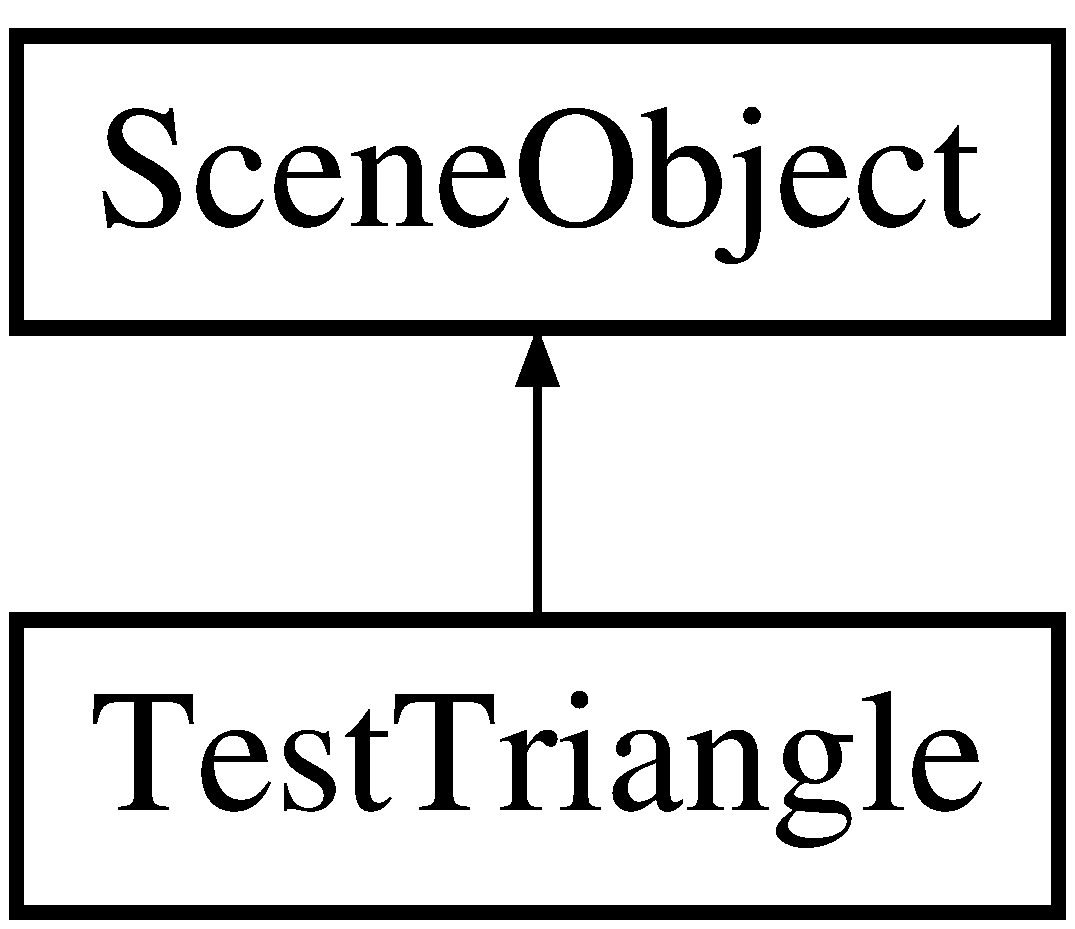
\includegraphics[height=2.000000cm]{class_scene_object}
\end{center}
\end{figure}
\subsection*{Public Types}
\begin{DoxyCompactItemize}
\item 
enum \hyperlink{class_scene_object_a3e12c3bc61287395d2fb63c370690dc9}{State} \{ \hyperlink{class_scene_object_a3e12c3bc61287395d2fb63c370690dc9ae7d31fc0602fb2ede144d18cdffd816b}{State\+::\+Ready}, 
\hyperlink{class_scene_object_a3e12c3bc61287395d2fb63c370690dc9a2ef54119c1f0d131a1a60e7776fa78f0}{State\+::\+Dying}, 
\hyperlink{class_scene_object_a3e12c3bc61287395d2fb63c370690dc9a183b62c7f067711f9c5a54913c054617}{State\+::\+Dead}
 \}\begin{DoxyCompactList}\small\item\em Enumeration for scene object lifetime states. \end{DoxyCompactList}
\end{DoxyCompactItemize}
\subsection*{Public Member Functions}
\begin{DoxyCompactItemize}
\item 
\hyperlink{class_scene_object_a4dc2616525cc46ff3138a6d10f600aad}{Scene\+Object} (\hyperlink{class_context}{Context} $\ast$context)
\begin{DoxyCompactList}\small\item\em Default constructor. \end{DoxyCompactList}\item 
virtual \hyperlink{class_scene_object_ab258d6b94e982d5ae71ad4d7652381f4}{$\sim$\+Scene\+Object} ()
\begin{DoxyCompactList}\small\item\em Default destructor. \end{DoxyCompactList}\item 
\hyperlink{class_scene_object_a3e12c3bc61287395d2fb63c370690dc9}{State} \hyperlink{class_scene_object_a8fd37f24e816c489f7af19510a4b5431}{get\+State} () const 
\begin{DoxyCompactList}\small\item\em Retrieve the current lifetime stage the object is in. \end{DoxyCompactList}\item 
void \hyperlink{class_scene_object_af1ce5eea77fe8015f3eeae73adbe0253}{set\+Dying} ()
\begin{DoxyCompactList}\small\item\em Set the scene object to begin the dying process. \end{DoxyCompactList}\item 
bool \hyperlink{class_scene_object_ab8635d3673dc8a91d71ba18402902314}{add\+Component} (std\+::shared\+\_\+ptr$<$ \hyperlink{class_scene_object_component}{Scene\+Object\+Component} $>$ component)
\begin{DoxyCompactList}\small\item\em Add a component to the scene object. \end{DoxyCompactList}\item 
std\+::shared\+\_\+ptr$<$ \hyperlink{class_scene_object_component}{Scene\+Object\+Component} $>$ \hyperlink{class_scene_object_a08c8437b836366cc1832f92af096ebc0}{get\+Component} (const std\+::string \&name)
\begin{DoxyCompactList}\small\item\em Access a component attached to the scene object. \end{DoxyCompactList}\item 
void \hyperlink{class_scene_object_af36a3463b19299b7d7cca2b476c36870}{set\+Position} (const glm\+::vec3 \&pos)
\begin{DoxyCompactList}\small\item\em Set the position of the entity within the scene. \end{DoxyCompactList}\item 
const glm\+::vec3 \& \hyperlink{class_scene_object_a91736aa3f5e06edb68c7c19ce9fbee85}{get\+Position} () const 
\begin{DoxyCompactList}\small\item\em Access the current position of the entity in the scene. \end{DoxyCompactList}\item 
void \hyperlink{class_scene_object_a07c1e8cb533c089560eb4d2cb319c629}{set\+Pitch} (G\+Lfloat angle)
\begin{DoxyCompactList}\small\item\em Set the pitch angle of the entity (\char`\"{}\+X-\/\+Axis Rotation\char`\"{}) \end{DoxyCompactList}\item 
G\+Lfloat \hyperlink{class_scene_object_a1a9a56ef5f3599892b14909dba70baa2}{get\+Pitch} () const 
\begin{DoxyCompactList}\small\item\em Get the pitch angle of the entity (\char`\"{}\+X-\/\+Axis Rotation\char`\"{}) \end{DoxyCompactList}\item 
void \hyperlink{class_scene_object_a92e89c65e5d427333919e7b6e5d1ce8c}{set\+Yaw} (G\+Lfloat angle)
\begin{DoxyCompactList}\small\item\em Set the yaw angle of the entity (\char`\"{}\+Y-\/\+Axis Rotation\char`\"{}) \end{DoxyCompactList}\item 
G\+Lfloat \hyperlink{class_scene_object_a61c445c541ab50f0f4e859d43926d71e}{get\+Yaw} () const 
\begin{DoxyCompactList}\small\item\em Get the yaw angle of the entity (\char`\"{}\+Y-\/\+Axis Rotation\char`\"{}) \end{DoxyCompactList}\item 
void \hyperlink{class_scene_object_aceabc31f66aa4929b7d7901da5660b1d}{set\+Roll} (G\+Lfloat angle)
\begin{DoxyCompactList}\small\item\em Set the roll angle of the entity (\char`\"{}\+Z-\/\+Axis Rotation\char`\"{}) \end{DoxyCompactList}\item 
G\+Lfloat \hyperlink{class_scene_object_a9c408db9660d645a86dd911abf96de11}{get\+Roll} () const 
\begin{DoxyCompactList}\small\item\em Get the roll angle of the entity (\char`\"{}\+Z-\/\+Axis Rotation\char`\"{}) \end{DoxyCompactList}\item 
void \hyperlink{class_scene_object_aece4f04fd597dd289c388b40fb9ed738}{set\+Rotations} (const glm\+::vec3 \&angles)
\begin{DoxyCompactList}\small\item\em Set all the rotation states of the entity at once. \end{DoxyCompactList}\item 
const glm\+::vec3 \& \hyperlink{class_scene_object_a1ff492a410e4338306462bae5f248ca1}{get\+Rotations} () const 
\begin{DoxyCompactList}\small\item\em Get all the rotation states of the entity at once. \end{DoxyCompactList}\item 
virtual void \hyperlink{class_scene_object_a5b69482cadd94997cd09bb145b1986d9}{step} (double dt)
\begin{DoxyCompactList}\small\item\em Step the simulation state. \end{DoxyCompactList}\item 
virtual void \hyperlink{class_scene_object_a2d5b85ae297772e2f5d0ef6fb920ddf2}{predraw} (\hyperlink{class_context}{Context} $\ast$context)
\begin{DoxyCompactList}\small\item\em Called before the renderer draws the scene This allows the scene objects to do updates that require a graphics context before the graphical state is drawn. \end{DoxyCompactList}\item 
void \hyperlink{class_scene_object_acbb90a879014f50ba44ad16e56436347}{update\+Model\+Matrix\+State} (\hyperlink{class_context}{Context} $\ast$context, std\+::shared\+\_\+ptr$<$ \hyperlink{class_shader_program}{Shader\+Program} $>$ shader) const 
\begin{DoxyCompactList}\small\item\em Use the standard position and rotation states as a model matrix This constructs a model matrix representing the position and rotation state, and tries to upload it into the u\+\_\+\+Model\+Matrix uniform in the presented shader, taking away the effort of doing this on every object from the programmers. \end{DoxyCompactList}\item 
virtual void \hyperlink{class_scene_object_a9dec6a34922a4063b561d3d16d396ee6}{draw} (\hyperlink{class_context}{Context} $\ast$context, std\+::shared\+\_\+ptr$<$ \hyperlink{class_shader_manager}{Shader\+Manager} $>$ shaders)=0
\begin{DoxyCompactList}\small\item\em Draw the object in its current state. \end{DoxyCompactList}\end{DoxyCompactItemize}
\subsection*{Private Attributes}
\begin{DoxyCompactItemize}
\item 
std\+::map$<$ std\+::string, std\+::shared\+\_\+ptr$<$ \hyperlink{class_scene_object_component}{Scene\+Object\+Component} $>$ $>$ \hyperlink{class_scene_object_a0e464a9eadb58928b80413b11437fa8b}{m\+\_\+\+Components}
\item 
glm\+::vec3 \hyperlink{class_scene_object_ad657befa8278678b73cafb62dec70b7a}{m\+\_\+\+Position}
\item 
glm\+::vec3 \hyperlink{class_scene_object_a925acd4f041f1f1796652cabf917ca90}{m\+\_\+\+Rotation}
\item 
\hyperlink{class_scene_object_a3e12c3bc61287395d2fb63c370690dc9}{State} \hyperlink{class_scene_object_a3648197f2a904ef0f7cc379ee0858e79}{m\+\_\+\+State}
\begin{DoxyCompactList}\small\item\em Current life-\/stage state. \end{DoxyCompactList}\end{DoxyCompactItemize}


\subsection{Detailed Description}
Abstract class for encapsulating self-\/management of scene entities. 

\begin{DoxyPrecond}{Precondition}
A valid Open\+GL context must be present to the program 
\end{DoxyPrecond}
\begin{DoxyAuthor}{Author}
Hayley Hatton 
\end{DoxyAuthor}
\begin{DoxyDate}{Date}
06/03/2016 
\end{DoxyDate}


Definition at line 14 of file Scene\+Object.\+h.



\subsection{Member Enumeration Documentation}
\index{Scene\+Object@{Scene\+Object}!State@{State}}
\index{State@{State}!Scene\+Object@{Scene\+Object}}
\subsubsection[{\texorpdfstring{State}{State}}]{\setlength{\rightskip}{0pt plus 5cm}enum {\bf Scene\+Object\+::\+State}\hspace{0.3cm}{\ttfamily [strong]}}\hypertarget{class_scene_object_a3e12c3bc61287395d2fb63c370690dc9}{}\label{class_scene_object_a3e12c3bc61287395d2fb63c370690dc9}


Enumeration for scene object lifetime states. 

\begin{Desc}
\item[Enumerator]\par
\begin{description}
\index{Ready@{Ready}!Scene\+Object@{Scene\+Object}}\index{Scene\+Object@{Scene\+Object}!Ready@{Ready}}\item[{\em 
Ready\hypertarget{class_scene_object_a3e12c3bc61287395d2fb63c370690dc9ae7d31fc0602fb2ede144d18cdffd816b}{}\label{class_scene_object_a3e12c3bc61287395d2fb63c370690dc9ae7d31fc0602fb2ede144d18cdffd816b}
}]Loaded and ready for use. \index{Dying@{Dying}!Scene\+Object@{Scene\+Object}}\index{Scene\+Object@{Scene\+Object}!Dying@{Dying}}\item[{\em 
Dying\hypertarget{class_scene_object_a3e12c3bc61287395d2fb63c370690dc9a2ef54119c1f0d131a1a60e7776fa78f0}{}\label{class_scene_object_a3e12c3bc61287395d2fb63c370690dc9a2ef54119c1f0d131a1a60e7776fa78f0}
}]Loaded, but marked as dead and needing cleanup. \index{Dead@{Dead}!Scene\+Object@{Scene\+Object}}\index{Scene\+Object@{Scene\+Object}!Dead@{Dead}}\item[{\em 
Dead\hypertarget{class_scene_object_a3e12c3bc61287395d2fb63c370690dc9a183b62c7f067711f9c5a54913c054617}{}\label{class_scene_object_a3e12c3bc61287395d2fb63c370690dc9a183b62c7f067711f9c5a54913c054617}
}]Cleaned up and finished; pending dtor. \end{description}
\end{Desc}


Definition at line 28 of file Scene\+Object.\+h.



\subsection{Constructor \& Destructor Documentation}
\index{Scene\+Object@{Scene\+Object}!Scene\+Object@{Scene\+Object}}
\index{Scene\+Object@{Scene\+Object}!Scene\+Object@{Scene\+Object}}
\subsubsection[{\texorpdfstring{Scene\+Object(\+Context $\ast$context)}{SceneObject(Context *context)}}]{\setlength{\rightskip}{0pt plus 5cm}Scene\+Object\+::\+Scene\+Object (
\begin{DoxyParamCaption}
\item[{{\bf Context} $\ast$}]{context}
\end{DoxyParamCaption}
)}\hypertarget{class_scene_object_a4dc2616525cc46ff3138a6d10f600aad}{}\label{class_scene_object_a4dc2616525cc46ff3138a6d10f600aad}


Default constructor. 


\begin{DoxyParams}{Parameters}
{\em context} & Graphics context \\
\hline
\end{DoxyParams}


Definition at line 6 of file Scene\+Object.\+cpp.

\index{Scene\+Object@{Scene\+Object}!````~Scene\+Object@{$\sim$\+Scene\+Object}}
\index{````~Scene\+Object@{$\sim$\+Scene\+Object}!Scene\+Object@{Scene\+Object}}
\subsubsection[{\texorpdfstring{$\sim$\+Scene\+Object()}{~SceneObject()}}]{\setlength{\rightskip}{0pt plus 5cm}Scene\+Object\+::$\sim$\+Scene\+Object (
\begin{DoxyParamCaption}
{}
\end{DoxyParamCaption}
)\hspace{0.3cm}{\ttfamily [virtual]}}\hypertarget{class_scene_object_ab258d6b94e982d5ae71ad4d7652381f4}{}\label{class_scene_object_ab258d6b94e982d5ae71ad4d7652381f4}


Default destructor. 



Definition at line 12 of file Scene\+Object.\+cpp.



\subsection{Member Function Documentation}
\index{Scene\+Object@{Scene\+Object}!add\+Component@{add\+Component}}
\index{add\+Component@{add\+Component}!Scene\+Object@{Scene\+Object}}
\subsubsection[{\texorpdfstring{add\+Component(std\+::shared\+\_\+ptr$<$ Scene\+Object\+Component $>$ component)}{addComponent(std::shared_ptr< SceneObjectComponent > component)}}]{\setlength{\rightskip}{0pt plus 5cm}bool Scene\+Object\+::add\+Component (
\begin{DoxyParamCaption}
\item[{std\+::shared\+\_\+ptr$<$ {\bf Scene\+Object\+Component} $>$}]{component}
\end{DoxyParamCaption}
)}\hypertarget{class_scene_object_ab8635d3673dc8a91d71ba18402902314}{}\label{class_scene_object_ab8635d3673dc8a91d71ba18402902314}


Add a component to the scene object. 


\begin{DoxyParams}{Parameters}
{\em component} & Smart pointer to the component \\
\hline
\end{DoxyParams}
\begin{DoxyReturn}{Returns}
True if added; false if already exists 
\end{DoxyReturn}


Definition at line 18 of file Scene\+Object.\+cpp.



References m\+\_\+\+Components.



Referenced by set\+Dying(), and Test\+Triangle\+::\+Test\+Triangle().

\index{Scene\+Object@{Scene\+Object}!draw@{draw}}
\index{draw@{draw}!Scene\+Object@{Scene\+Object}}
\subsubsection[{\texorpdfstring{draw(\+Context $\ast$context, std\+::shared\+\_\+ptr$<$ Shader\+Manager $>$ shaders)=0}{draw(Context *context, std::shared_ptr< ShaderManager > shaders)=0}}]{\setlength{\rightskip}{0pt plus 5cm}virtual void Scene\+Object\+::draw (
\begin{DoxyParamCaption}
\item[{{\bf Context} $\ast$}]{context, }
\item[{std\+::shared\+\_\+ptr$<$ {\bf Shader\+Manager} $>$}]{shaders}
\end{DoxyParamCaption}
)\hspace{0.3cm}{\ttfamily [pure virtual]}}\hypertarget{class_scene_object_a9dec6a34922a4063b561d3d16d396ee6}{}\label{class_scene_object_a9dec6a34922a4063b561d3d16d396ee6}


Draw the object in its current state. 


\begin{DoxyParams}{Parameters}
{\em context} & Graphics context \\
\hline
{\em shaders} & Shader manager containing shader programs for use \\
\hline
\end{DoxyParams}


Implemented in \hyperlink{class_test_triangle_aadf5ec7f41246e3c114e7f44f009f303}{Test\+Triangle}.



Referenced by get\+Rotations().

\index{Scene\+Object@{Scene\+Object}!get\+Component@{get\+Component}}
\index{get\+Component@{get\+Component}!Scene\+Object@{Scene\+Object}}
\subsubsection[{\texorpdfstring{get\+Component(const std\+::string \&name)}{getComponent(const std::string &name)}}]{\setlength{\rightskip}{0pt plus 5cm}std\+::shared\+\_\+ptr$<$ {\bf Scene\+Object\+Component} $>$ Scene\+Object\+::get\+Component (
\begin{DoxyParamCaption}
\item[{const std\+::string \&}]{name}
\end{DoxyParamCaption}
)}\hypertarget{class_scene_object_a08c8437b836366cc1832f92af096ebc0}{}\label{class_scene_object_a08c8437b836366cc1832f92af096ebc0}


Access a component attached to the scene object. 


\begin{DoxyParams}{Parameters}
{\em name} & Identifying name of the component type \\
\hline
\end{DoxyParams}
\begin{DoxyReturn}{Returns}
Smart pointer to the component; nullptr if none of that type 
\end{DoxyReturn}


Definition at line 30 of file Scene\+Object.\+cpp.



References m\+\_\+\+Components.



Referenced by set\+Dying().

\index{Scene\+Object@{Scene\+Object}!get\+Pitch@{get\+Pitch}}
\index{get\+Pitch@{get\+Pitch}!Scene\+Object@{Scene\+Object}}
\subsubsection[{\texorpdfstring{get\+Pitch() const }{getPitch() const }}]{\setlength{\rightskip}{0pt plus 5cm}G\+Lfloat Scene\+Object\+::get\+Pitch (
\begin{DoxyParamCaption}
{}
\end{DoxyParamCaption}
) const\hspace{0.3cm}{\ttfamily [inline]}}\hypertarget{class_scene_object_a1a9a56ef5f3599892b14909dba70baa2}{}\label{class_scene_object_a1a9a56ef5f3599892b14909dba70baa2}


Get the pitch angle of the entity (\char`\"{}\+X-\/\+Axis Rotation\char`\"{}) 

\begin{DoxyReturn}{Returns}
Current pitch angle 
\end{DoxyReturn}


Definition at line 80 of file Scene\+Object.\+h.



References m\+\_\+\+Rotation.

\index{Scene\+Object@{Scene\+Object}!get\+Position@{get\+Position}}
\index{get\+Position@{get\+Position}!Scene\+Object@{Scene\+Object}}
\subsubsection[{\texorpdfstring{get\+Position() const }{getPosition() const }}]{\setlength{\rightskip}{0pt plus 5cm}const glm\+::vec3\& Scene\+Object\+::get\+Position (
\begin{DoxyParamCaption}
{}
\end{DoxyParamCaption}
) const\hspace{0.3cm}{\ttfamily [inline]}}\hypertarget{class_scene_object_a91736aa3f5e06edb68c7c19ce9fbee85}{}\label{class_scene_object_a91736aa3f5e06edb68c7c19ce9fbee85}


Access the current position of the entity in the scene. 

\begin{DoxyReturn}{Returns}
Current position 
\end{DoxyReturn}


Definition at line 68 of file Scene\+Object.\+h.



References m\+\_\+\+Position.

\index{Scene\+Object@{Scene\+Object}!get\+Roll@{get\+Roll}}
\index{get\+Roll@{get\+Roll}!Scene\+Object@{Scene\+Object}}
\subsubsection[{\texorpdfstring{get\+Roll() const }{getRoll() const }}]{\setlength{\rightskip}{0pt plus 5cm}G\+Lfloat Scene\+Object\+::get\+Roll (
\begin{DoxyParamCaption}
{}
\end{DoxyParamCaption}
) const\hspace{0.3cm}{\ttfamily [inline]}}\hypertarget{class_scene_object_a9c408db9660d645a86dd911abf96de11}{}\label{class_scene_object_a9c408db9660d645a86dd911abf96de11}


Get the roll angle of the entity (\char`\"{}\+Z-\/\+Axis Rotation\char`\"{}) 

\begin{DoxyReturn}{Returns}
Current roll angle 
\end{DoxyReturn}


Definition at line 104 of file Scene\+Object.\+h.



References m\+\_\+\+Rotation.

\index{Scene\+Object@{Scene\+Object}!get\+Rotations@{get\+Rotations}}
\index{get\+Rotations@{get\+Rotations}!Scene\+Object@{Scene\+Object}}
\subsubsection[{\texorpdfstring{get\+Rotations() const }{getRotations() const }}]{\setlength{\rightskip}{0pt plus 5cm}const glm\+::vec3\& Scene\+Object\+::get\+Rotations (
\begin{DoxyParamCaption}
{}
\end{DoxyParamCaption}
) const\hspace{0.3cm}{\ttfamily [inline]}}\hypertarget{class_scene_object_a1ff492a410e4338306462bae5f248ca1}{}\label{class_scene_object_a1ff492a410e4338306462bae5f248ca1}


Get all the rotation states of the entity at once. 

\begin{DoxyReturn}{Returns}
Current rotation angles as a vector 
\end{DoxyReturn}


Definition at line 116 of file Scene\+Object.\+h.



References draw(), m\+\_\+\+Rotation, predraw(), step(), and update\+Model\+Matrix\+State().

\index{Scene\+Object@{Scene\+Object}!get\+State@{get\+State}}
\index{get\+State@{get\+State}!Scene\+Object@{Scene\+Object}}
\subsubsection[{\texorpdfstring{get\+State() const }{getState() const }}]{\setlength{\rightskip}{0pt plus 5cm}{\bf State} Scene\+Object\+::get\+State (
\begin{DoxyParamCaption}
{}
\end{DoxyParamCaption}
) const\hspace{0.3cm}{\ttfamily [inline]}}\hypertarget{class_scene_object_a8fd37f24e816c489f7af19510a4b5431}{}\label{class_scene_object_a8fd37f24e816c489f7af19510a4b5431}


Retrieve the current lifetime stage the object is in. 

\begin{DoxyReturn}{Returns}
Current life-\/stage state 
\end{DoxyReturn}


Definition at line 39 of file Scene\+Object.\+h.



References m\+\_\+\+State.

\index{Scene\+Object@{Scene\+Object}!get\+Yaw@{get\+Yaw}}
\index{get\+Yaw@{get\+Yaw}!Scene\+Object@{Scene\+Object}}
\subsubsection[{\texorpdfstring{get\+Yaw() const }{getYaw() const }}]{\setlength{\rightskip}{0pt plus 5cm}G\+Lfloat Scene\+Object\+::get\+Yaw (
\begin{DoxyParamCaption}
{}
\end{DoxyParamCaption}
) const\hspace{0.3cm}{\ttfamily [inline]}}\hypertarget{class_scene_object_a61c445c541ab50f0f4e859d43926d71e}{}\label{class_scene_object_a61c445c541ab50f0f4e859d43926d71e}


Get the yaw angle of the entity (\char`\"{}\+Y-\/\+Axis Rotation\char`\"{}) 

\begin{DoxyReturn}{Returns}
Current yaw angle 
\end{DoxyReturn}


Definition at line 92 of file Scene\+Object.\+h.



References m\+\_\+\+Rotation.

\index{Scene\+Object@{Scene\+Object}!predraw@{predraw}}
\index{predraw@{predraw}!Scene\+Object@{Scene\+Object}}
\subsubsection[{\texorpdfstring{predraw(\+Context $\ast$context)}{predraw(Context *context)}}]{\setlength{\rightskip}{0pt plus 5cm}void Scene\+Object\+::predraw (
\begin{DoxyParamCaption}
\item[{{\bf Context} $\ast$}]{context}
\end{DoxyParamCaption}
)\hspace{0.3cm}{\ttfamily [virtual]}}\hypertarget{class_scene_object_a2d5b85ae297772e2f5d0ef6fb920ddf2}{}\label{class_scene_object_a2d5b85ae297772e2f5d0ef6fb920ddf2}


Called before the renderer draws the scene This allows the scene objects to do updates that require a graphics context before the graphical state is drawn. 


\begin{DoxyParams}{Parameters}
{\em context} & Graphics context \\
\hline
\end{DoxyParams}


Reimplemented in \hyperlink{class_test_triangle_a0b7b66d114a3d97e524f2d8d9f13a9e7}{Test\+Triangle}.



Definition at line 45 of file Scene\+Object.\+cpp.



References m\+\_\+\+Components.



Referenced by get\+Rotations(), and Test\+Triangle\+::predraw().

\index{Scene\+Object@{Scene\+Object}!set\+Dying@{set\+Dying}}
\index{set\+Dying@{set\+Dying}!Scene\+Object@{Scene\+Object}}
\subsubsection[{\texorpdfstring{set\+Dying()}{setDying()}}]{\setlength{\rightskip}{0pt plus 5cm}void Scene\+Object\+::set\+Dying (
\begin{DoxyParamCaption}
{}
\end{DoxyParamCaption}
)\hspace{0.3cm}{\ttfamily [inline]}}\hypertarget{class_scene_object_af1ce5eea77fe8015f3eeae73adbe0253}{}\label{class_scene_object_af1ce5eea77fe8015f3eeae73adbe0253}


Set the scene object to begin the dying process. 



Definition at line 42 of file Scene\+Object.\+h.



References add\+Component(), Dying, get\+Component(), and m\+\_\+\+State.



Referenced by Test\+Triangle\+::on\+Message().

\index{Scene\+Object@{Scene\+Object}!set\+Pitch@{set\+Pitch}}
\index{set\+Pitch@{set\+Pitch}!Scene\+Object@{Scene\+Object}}
\subsubsection[{\texorpdfstring{set\+Pitch(\+G\+Lfloat angle)}{setPitch(GLfloat angle)}}]{\setlength{\rightskip}{0pt plus 5cm}void Scene\+Object\+::set\+Pitch (
\begin{DoxyParamCaption}
\item[{G\+Lfloat}]{angle}
\end{DoxyParamCaption}
)\hspace{0.3cm}{\ttfamily [inline]}}\hypertarget{class_scene_object_a07c1e8cb533c089560eb4d2cb319c629}{}\label{class_scene_object_a07c1e8cb533c089560eb4d2cb319c629}


Set the pitch angle of the entity (\char`\"{}\+X-\/\+Axis Rotation\char`\"{}) 


\begin{DoxyParams}{Parameters}
{\em angle} & New pitch angle \\
\hline
\end{DoxyParams}


Definition at line 74 of file Scene\+Object.\+h.



References m\+\_\+\+Rotation.

\index{Scene\+Object@{Scene\+Object}!set\+Position@{set\+Position}}
\index{set\+Position@{set\+Position}!Scene\+Object@{Scene\+Object}}
\subsubsection[{\texorpdfstring{set\+Position(const glm\+::vec3 \&pos)}{setPosition(const glm::vec3 &pos)}}]{\setlength{\rightskip}{0pt plus 5cm}void Scene\+Object\+::set\+Position (
\begin{DoxyParamCaption}
\item[{const glm\+::vec3 \&}]{pos}
\end{DoxyParamCaption}
)\hspace{0.3cm}{\ttfamily [inline]}}\hypertarget{class_scene_object_af36a3463b19299b7d7cca2b476c36870}{}\label{class_scene_object_af36a3463b19299b7d7cca2b476c36870}


Set the position of the entity within the scene. 


\begin{DoxyParams}{Parameters}
{\em pos} & New position \\
\hline
\end{DoxyParams}


Definition at line 62 of file Scene\+Object.\+h.



References m\+\_\+\+Position.

\index{Scene\+Object@{Scene\+Object}!set\+Roll@{set\+Roll}}
\index{set\+Roll@{set\+Roll}!Scene\+Object@{Scene\+Object}}
\subsubsection[{\texorpdfstring{set\+Roll(\+G\+Lfloat angle)}{setRoll(GLfloat angle)}}]{\setlength{\rightskip}{0pt plus 5cm}void Scene\+Object\+::set\+Roll (
\begin{DoxyParamCaption}
\item[{G\+Lfloat}]{angle}
\end{DoxyParamCaption}
)\hspace{0.3cm}{\ttfamily [inline]}}\hypertarget{class_scene_object_aceabc31f66aa4929b7d7901da5660b1d}{}\label{class_scene_object_aceabc31f66aa4929b7d7901da5660b1d}


Set the roll angle of the entity (\char`\"{}\+Z-\/\+Axis Rotation\char`\"{}) 


\begin{DoxyParams}{Parameters}
{\em angle} & New roll angle \\
\hline
\end{DoxyParams}


Definition at line 98 of file Scene\+Object.\+h.



References m\+\_\+\+Rotation.

\index{Scene\+Object@{Scene\+Object}!set\+Rotations@{set\+Rotations}}
\index{set\+Rotations@{set\+Rotations}!Scene\+Object@{Scene\+Object}}
\subsubsection[{\texorpdfstring{set\+Rotations(const glm\+::vec3 \&angles)}{setRotations(const glm::vec3 &angles)}}]{\setlength{\rightskip}{0pt plus 5cm}void Scene\+Object\+::set\+Rotations (
\begin{DoxyParamCaption}
\item[{const glm\+::vec3 \&}]{angles}
\end{DoxyParamCaption}
)\hspace{0.3cm}{\ttfamily [inline]}}\hypertarget{class_scene_object_aece4f04fd597dd289c388b40fb9ed738}{}\label{class_scene_object_aece4f04fd597dd289c388b40fb9ed738}


Set all the rotation states of the entity at once. 


\begin{DoxyParams}{Parameters}
{\em angles} & New rotation angles as a vector \\
\hline
\end{DoxyParams}


Definition at line 110 of file Scene\+Object.\+h.



References m\+\_\+\+Rotation.

\index{Scene\+Object@{Scene\+Object}!set\+Yaw@{set\+Yaw}}
\index{set\+Yaw@{set\+Yaw}!Scene\+Object@{Scene\+Object}}
\subsubsection[{\texorpdfstring{set\+Yaw(\+G\+Lfloat angle)}{setYaw(GLfloat angle)}}]{\setlength{\rightskip}{0pt plus 5cm}void Scene\+Object\+::set\+Yaw (
\begin{DoxyParamCaption}
\item[{G\+Lfloat}]{angle}
\end{DoxyParamCaption}
)\hspace{0.3cm}{\ttfamily [inline]}}\hypertarget{class_scene_object_a92e89c65e5d427333919e7b6e5d1ce8c}{}\label{class_scene_object_a92e89c65e5d427333919e7b6e5d1ce8c}


Set the yaw angle of the entity (\char`\"{}\+Y-\/\+Axis Rotation\char`\"{}) 


\begin{DoxyParams}{Parameters}
{\em angle} & New yaw angle \\
\hline
\end{DoxyParams}


Definition at line 86 of file Scene\+Object.\+h.



References m\+\_\+\+Rotation.

\index{Scene\+Object@{Scene\+Object}!step@{step}}
\index{step@{step}!Scene\+Object@{Scene\+Object}}
\subsubsection[{\texorpdfstring{step(double dt)}{step(double dt)}}]{\setlength{\rightskip}{0pt plus 5cm}void Scene\+Object\+::step (
\begin{DoxyParamCaption}
\item[{double}]{dt}
\end{DoxyParamCaption}
)\hspace{0.3cm}{\ttfamily [virtual]}}\hypertarget{class_scene_object_a5b69482cadd94997cd09bb145b1986d9}{}\label{class_scene_object_a5b69482cadd94997cd09bb145b1986d9}


Step the simulation state. 


\begin{DoxyParams}{Parameters}
{\em dt} & Delta-\/time since last step call in seconds \\
\hline
\end{DoxyParams}


Reimplemented in \hyperlink{class_test_triangle_a99c4fb3e4da6d1dabf3f9cdeef5b1b31}{Test\+Triangle}.



Definition at line 39 of file Scene\+Object.\+cpp.



References m\+\_\+\+Components.



Referenced by get\+Rotations(), and Test\+Triangle\+::step().

\index{Scene\+Object@{Scene\+Object}!update\+Model\+Matrix\+State@{update\+Model\+Matrix\+State}}
\index{update\+Model\+Matrix\+State@{update\+Model\+Matrix\+State}!Scene\+Object@{Scene\+Object}}
\subsubsection[{\texorpdfstring{update\+Model\+Matrix\+State(\+Context $\ast$context, std\+::shared\+\_\+ptr$<$ Shader\+Program $>$ shader) const }{updateModelMatrixState(Context *context, std::shared_ptr< ShaderProgram > shader) const }}]{\setlength{\rightskip}{0pt plus 5cm}void Scene\+Object\+::update\+Model\+Matrix\+State (
\begin{DoxyParamCaption}
\item[{{\bf Context} $\ast$}]{context, }
\item[{std\+::shared\+\_\+ptr$<$ {\bf Shader\+Program} $>$}]{shader}
\end{DoxyParamCaption}
) const}\hypertarget{class_scene_object_acbb90a879014f50ba44ad16e56436347}{}\label{class_scene_object_acbb90a879014f50ba44ad16e56436347}


Use the standard position and rotation states as a model matrix This constructs a model matrix representing the position and rotation state, and tries to upload it into the u\+\_\+\+Model\+Matrix uniform in the presented shader, taking away the effort of doing this on every object from the programmers. 


\begin{DoxyParams}{Parameters}
{\em context} & Graphics context \\
\hline
{\em shader} & Shader program to upload model matrix to \\
\hline
\end{DoxyParams}


Definition at line 51 of file Scene\+Object.\+cpp.



References m\+\_\+\+Position, and m\+\_\+\+Rotation.



Referenced by get\+Rotations().



\subsection{Member Data Documentation}
\index{Scene\+Object@{Scene\+Object}!m\+\_\+\+Components@{m\+\_\+\+Components}}
\index{m\+\_\+\+Components@{m\+\_\+\+Components}!Scene\+Object@{Scene\+Object}}
\subsubsection[{\texorpdfstring{m\+\_\+\+Components}{m_Components}}]{\setlength{\rightskip}{0pt plus 5cm}std\+::map$<$std\+::string, std\+::shared\+\_\+ptr$<${\bf Scene\+Object\+Component}$>$ $>$ Scene\+Object\+::m\+\_\+\+Components\hspace{0.3cm}{\ttfamily [private]}}\hypertarget{class_scene_object_a0e464a9eadb58928b80413b11437fa8b}{}\label{class_scene_object_a0e464a9eadb58928b80413b11437fa8b}


Definition at line 155 of file Scene\+Object.\+h.



Referenced by add\+Component(), get\+Component(), predraw(), and step().

\index{Scene\+Object@{Scene\+Object}!m\+\_\+\+Position@{m\+\_\+\+Position}}
\index{m\+\_\+\+Position@{m\+\_\+\+Position}!Scene\+Object@{Scene\+Object}}
\subsubsection[{\texorpdfstring{m\+\_\+\+Position}{m_Position}}]{\setlength{\rightskip}{0pt plus 5cm}glm\+::vec3 Scene\+Object\+::m\+\_\+\+Position\hspace{0.3cm}{\ttfamily [private]}}\hypertarget{class_scene_object_ad657befa8278678b73cafb62dec70b7a}{}\label{class_scene_object_ad657befa8278678b73cafb62dec70b7a}


Definition at line 156 of file Scene\+Object.\+h.



Referenced by get\+Position(), set\+Position(), and update\+Model\+Matrix\+State().

\index{Scene\+Object@{Scene\+Object}!m\+\_\+\+Rotation@{m\+\_\+\+Rotation}}
\index{m\+\_\+\+Rotation@{m\+\_\+\+Rotation}!Scene\+Object@{Scene\+Object}}
\subsubsection[{\texorpdfstring{m\+\_\+\+Rotation}{m_Rotation}}]{\setlength{\rightskip}{0pt plus 5cm}glm\+::vec3 Scene\+Object\+::m\+\_\+\+Rotation\hspace{0.3cm}{\ttfamily [private]}}\hypertarget{class_scene_object_a925acd4f041f1f1796652cabf917ca90}{}\label{class_scene_object_a925acd4f041f1f1796652cabf917ca90}


Definition at line 157 of file Scene\+Object.\+h.



Referenced by get\+Pitch(), get\+Roll(), get\+Rotations(), get\+Yaw(), set\+Pitch(), set\+Roll(), set\+Rotations(), set\+Yaw(), and update\+Model\+Matrix\+State().

\index{Scene\+Object@{Scene\+Object}!m\+\_\+\+State@{m\+\_\+\+State}}
\index{m\+\_\+\+State@{m\+\_\+\+State}!Scene\+Object@{Scene\+Object}}
\subsubsection[{\texorpdfstring{m\+\_\+\+State}{m_State}}]{\setlength{\rightskip}{0pt plus 5cm}{\bf State} Scene\+Object\+::m\+\_\+\+State\hspace{0.3cm}{\ttfamily [private]}}\hypertarget{class_scene_object_a3648197f2a904ef0f7cc379ee0858e79}{}\label{class_scene_object_a3648197f2a904ef0f7cc379ee0858e79}


Current life-\/stage state. 



Definition at line 158 of file Scene\+Object.\+h.



Referenced by get\+State(), and set\+Dying().



The documentation for this class was generated from the following files\+:\begin{DoxyCompactItemize}
\item 
Lunar\+Drift/engine/containers/\hyperlink{_scene_object_8h}{Scene\+Object.\+h}\item 
Lunar\+Drift/engine/containers/\hyperlink{_scene_object_8cpp}{Scene\+Object.\+cpp}\end{DoxyCompactItemize}

\hypertarget{class_scene_object_component}{}\section{Scene\+Object\+Component Class Reference}
\label{class_scene_object_component}\index{Scene\+Object\+Component@{Scene\+Object\+Component}}


Base class for components that are to be attached to scene objects.  




{\ttfamily \#include $<$Scene\+Object\+Component.\+h$>$}

Inheritance diagram for Scene\+Object\+Component\+:\begin{figure}[H]
\begin{center}
\leavevmode
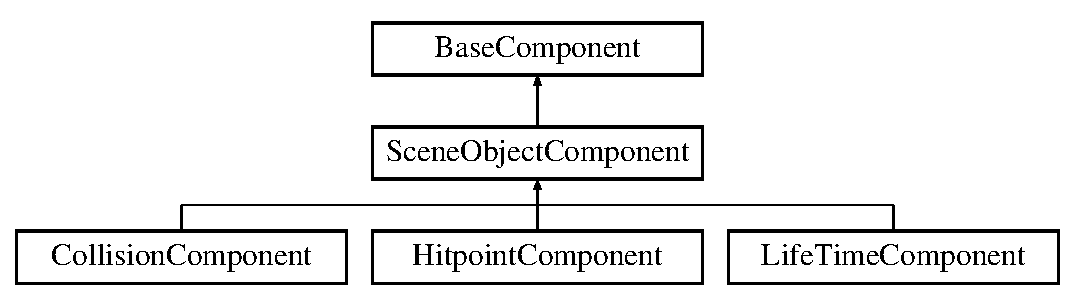
\includegraphics[height=3.000000cm]{class_scene_object_component}
\end{center}
\end{figure}
\subsection*{Public Member Functions}
\begin{DoxyCompactItemize}
\item 
\hyperlink{class_scene_object_component_a8bcfb5bc3d3bdb01faa9ad1286b8585f}{Scene\+Object\+Component} (const std\+::string \&name, \hyperlink{class_scene_object}{Scene\+Object} $\ast$parent, std\+::weak\+\_\+ptr$<$ \hyperlink{class_meta_manager}{Meta\+Manager} $>$ managers)
\begin{DoxyCompactList}\small\item\em Default constructor. \end{DoxyCompactList}\item 
virtual \hyperlink{class_scene_object_component_a2832eebdd71efb588d47be60ba95e49f}{$\sim$\+Scene\+Object\+Component} ()
\begin{DoxyCompactList}\small\item\em Default destructor. \end{DoxyCompactList}\item 
virtual void \hyperlink{class_scene_object_component_a99ebed011a6547be4d31a09927e3b810}{step} (double dt)=0
\begin{DoxyCompactList}\small\item\em Step the simulation state. \end{DoxyCompactList}\item 
virtual void \hyperlink{class_scene_object_component_a7110e37ad23a708c2bf9828c7fd7df2f}{predraw} (\hyperlink{class_context}{Context} $\ast$context)=0
\begin{DoxyCompactList}\small\item\em Called before the renderer draws the scene This allows the scene objects to do updates that require a graphics context before the graphical state is drawn. \end{DoxyCompactList}\item 
\hyperlink{class_scene_object}{Scene\+Object} $\ast$ \hyperlink{class_scene_object_component_ab4e4f580e5257b8f9064f7b594b97ac9}{get\+Parent} ()
\begin{DoxyCompactList}\small\item\em Access the parent class that owns this component. \end{DoxyCompactList}\item 
std\+::weak\+\_\+ptr$<$ \hyperlink{class_meta_manager}{Meta\+Manager} $>$ \hyperlink{class_scene_object_component_a6b2b0732ce70a245bbea15d6ad58f35d}{get\+Meta\+Manager} ()
\begin{DoxyCompactList}\small\item\em Access the metamanager for the scene that the parent is a part of. \end{DoxyCompactList}\end{DoxyCompactItemize}
\subsection*{Protected Attributes}
\begin{DoxyCompactItemize}
\item 
std\+::weak\+\_\+ptr$<$ \hyperlink{class_meta_manager}{Meta\+Manager} $>$ \hyperlink{class_scene_object_component_ae37257f842b003aa25ca634565d2f1e4}{m\+\_\+\+Managers}
\begin{DoxyCompactList}\small\item\em \hyperlink{class_scene}{Scene}\textquotesingle{}s managers. \end{DoxyCompactList}\end{DoxyCompactItemize}
\subsection*{Private Attributes}
\begin{DoxyCompactItemize}
\item 
\hyperlink{class_scene_object}{Scene\+Object} $\ast$ \hyperlink{class_scene_object_component_ad7992ff4976be980767939e44eba2b2f}{m\+\_\+\+Parent}
\begin{DoxyCompactList}\small\item\em Class that has ownership of this component. \end{DoxyCompactList}\end{DoxyCompactItemize}


\subsection{Detailed Description}
Base class for components that are to be attached to scene objects. 

\begin{DoxyAuthor}{Author}
Hayley Hatton 
\end{DoxyAuthor}
\begin{DoxyDate}{Date}
06/03/2016 
\end{DoxyDate}


Definition at line 15 of file Scene\+Object\+Component.\+h.



\subsection{Constructor \& Destructor Documentation}
\index{Scene\+Object\+Component@{Scene\+Object\+Component}!Scene\+Object\+Component@{Scene\+Object\+Component}}
\index{Scene\+Object\+Component@{Scene\+Object\+Component}!Scene\+Object\+Component@{Scene\+Object\+Component}}
\subsubsection[{\texorpdfstring{Scene\+Object\+Component(const std\+::string \&name, Scene\+Object $\ast$parent, std\+::weak\+\_\+ptr$<$ Meta\+Manager $>$ managers)}{SceneObjectComponent(const std::string &name, SceneObject *parent, std::weak_ptr< MetaManager > managers)}}]{\setlength{\rightskip}{0pt plus 5cm}Scene\+Object\+Component\+::\+Scene\+Object\+Component (
\begin{DoxyParamCaption}
\item[{const std\+::string \&}]{name, }
\item[{{\bf Scene\+Object} $\ast$}]{parent, }
\item[{std\+::weak\+\_\+ptr$<$ {\bf Meta\+Manager} $>$}]{managers}
\end{DoxyParamCaption}
)}\hypertarget{class_scene_object_component_a8bcfb5bc3d3bdb01faa9ad1286b8585f}{}\label{class_scene_object_component_a8bcfb5bc3d3bdb01faa9ad1286b8585f}


Default constructor. 


\begin{DoxyParams}{Parameters}
{\em name} & Identifying name of the component class \\
\hline
{\em parent} & Pointer to the scene object to attach component to \\
\hline
{\em managers} & Metamanager for accessing scene\textquotesingle{}s managers \\
\hline
\end{DoxyParams}


Definition at line 5 of file Scene\+Object\+Component.\+cpp.

\index{Scene\+Object\+Component@{Scene\+Object\+Component}!````~Scene\+Object\+Component@{$\sim$\+Scene\+Object\+Component}}
\index{````~Scene\+Object\+Component@{$\sim$\+Scene\+Object\+Component}!Scene\+Object\+Component@{Scene\+Object\+Component}}
\subsubsection[{\texorpdfstring{$\sim$\+Scene\+Object\+Component()}{~SceneObjectComponent()}}]{\setlength{\rightskip}{0pt plus 5cm}Scene\+Object\+Component\+::$\sim$\+Scene\+Object\+Component (
\begin{DoxyParamCaption}
{}
\end{DoxyParamCaption}
)\hspace{0.3cm}{\ttfamily [virtual]}}\hypertarget{class_scene_object_component_a2832eebdd71efb588d47be60ba95e49f}{}\label{class_scene_object_component_a2832eebdd71efb588d47be60ba95e49f}


Default destructor. 



Definition at line 16 of file Scene\+Object\+Component.\+cpp.



\subsection{Member Function Documentation}
\index{Scene\+Object\+Component@{Scene\+Object\+Component}!get\+Meta\+Manager@{get\+Meta\+Manager}}
\index{get\+Meta\+Manager@{get\+Meta\+Manager}!Scene\+Object\+Component@{Scene\+Object\+Component}}
\subsubsection[{\texorpdfstring{get\+Meta\+Manager()}{getMetaManager()}}]{\setlength{\rightskip}{0pt plus 5cm}std\+::weak\+\_\+ptr$<${\bf Meta\+Manager}$>$ Scene\+Object\+Component\+::get\+Meta\+Manager (
\begin{DoxyParamCaption}
{}
\end{DoxyParamCaption}
)\hspace{0.3cm}{\ttfamily [inline]}}\hypertarget{class_scene_object_component_a6b2b0732ce70a245bbea15d6ad58f35d}{}\label{class_scene_object_component_a6b2b0732ce70a245bbea15d6ad58f35d}


Access the metamanager for the scene that the parent is a part of. 

\begin{DoxyReturn}{Returns}
Weakly-\/referenced pointer to the owning scene\textquotesingle{}s metamanager 
\end{DoxyReturn}


Definition at line 57 of file Scene\+Object\+Component.\+h.



References m\+\_\+\+Managers.

\index{Scene\+Object\+Component@{Scene\+Object\+Component}!get\+Parent@{get\+Parent}}
\index{get\+Parent@{get\+Parent}!Scene\+Object\+Component@{Scene\+Object\+Component}}
\subsubsection[{\texorpdfstring{get\+Parent()}{getParent()}}]{\setlength{\rightskip}{0pt plus 5cm}{\bf Scene\+Object}$\ast$ Scene\+Object\+Component\+::get\+Parent (
\begin{DoxyParamCaption}
{}
\end{DoxyParamCaption}
)\hspace{0.3cm}{\ttfamily [inline]}}\hypertarget{class_scene_object_component_ab4e4f580e5257b8f9064f7b594b97ac9}{}\label{class_scene_object_component_ab4e4f580e5257b8f9064f7b594b97ac9}


Access the parent class that owns this component. 

\begin{DoxyReturn}{Returns}
Reference to the parent class 
\end{DoxyReturn}


Definition at line 51 of file Scene\+Object\+Component.\+h.



References m\+\_\+\+Parent.



Referenced by Collision\+Component\+::\+Collision\+Component(), Hitpoint\+Component\+::on\+Message(), Life\+Time\+Component\+::step(), and Collision\+Component\+::$\sim$\+Collision\+Component().

\index{Scene\+Object\+Component@{Scene\+Object\+Component}!predraw@{predraw}}
\index{predraw@{predraw}!Scene\+Object\+Component@{Scene\+Object\+Component}}
\subsubsection[{\texorpdfstring{predraw(\+Context $\ast$context)=0}{predraw(Context *context)=0}}]{\setlength{\rightskip}{0pt plus 5cm}virtual void Scene\+Object\+Component\+::predraw (
\begin{DoxyParamCaption}
\item[{{\bf Context} $\ast$}]{context}
\end{DoxyParamCaption}
)\hspace{0.3cm}{\ttfamily [pure virtual]}}\hypertarget{class_scene_object_component_a7110e37ad23a708c2bf9828c7fd7df2f}{}\label{class_scene_object_component_a7110e37ad23a708c2bf9828c7fd7df2f}


Called before the renderer draws the scene This allows the scene objects to do updates that require a graphics context before the graphical state is drawn. 


\begin{DoxyParams}{Parameters}
{\em context} & Graphics context \\
\hline
\end{DoxyParams}


Implemented in \hyperlink{class_collision_component_a322c2d4550aef70b8284465ae34278db}{Collision\+Component}, \hyperlink{class_life_time_component_a206515c60de0d9bc07062daf8d24446e}{Life\+Time\+Component}, and \hyperlink{class_hitpoint_component_a3210abfca24e1bc9827f56533ab798af}{Hitpoint\+Component}.

\index{Scene\+Object\+Component@{Scene\+Object\+Component}!step@{step}}
\index{step@{step}!Scene\+Object\+Component@{Scene\+Object\+Component}}
\subsubsection[{\texorpdfstring{step(double dt)=0}{step(double dt)=0}}]{\setlength{\rightskip}{0pt plus 5cm}virtual void Scene\+Object\+Component\+::step (
\begin{DoxyParamCaption}
\item[{double}]{dt}
\end{DoxyParamCaption}
)\hspace{0.3cm}{\ttfamily [pure virtual]}}\hypertarget{class_scene_object_component_a99ebed011a6547be4d31a09927e3b810}{}\label{class_scene_object_component_a99ebed011a6547be4d31a09927e3b810}


Step the simulation state. 


\begin{DoxyParams}{Parameters}
{\em dt} & Delta-\/time since last step call in seconds \\
\hline
\end{DoxyParams}


Implemented in \hyperlink{class_collision_component_aee9d681edd938781127af2249b750125}{Collision\+Component}, \hyperlink{class_life_time_component_a709b9485f9bce5c7a6cec8f000bcb905}{Life\+Time\+Component}, and \hyperlink{class_hitpoint_component_ab293fcc4d167a4fa9cd27cbf1ba42018}{Hitpoint\+Component}.



\subsection{Member Data Documentation}
\index{Scene\+Object\+Component@{Scene\+Object\+Component}!m\+\_\+\+Managers@{m\+\_\+\+Managers}}
\index{m\+\_\+\+Managers@{m\+\_\+\+Managers}!Scene\+Object\+Component@{Scene\+Object\+Component}}
\subsubsection[{\texorpdfstring{m\+\_\+\+Managers}{m_Managers}}]{\setlength{\rightskip}{0pt plus 5cm}std\+::weak\+\_\+ptr$<${\bf Meta\+Manager}$>$ Scene\+Object\+Component\+::m\+\_\+\+Managers\hspace{0.3cm}{\ttfamily [protected]}}\hypertarget{class_scene_object_component_ae37257f842b003aa25ca634565d2f1e4}{}\label{class_scene_object_component_ae37257f842b003aa25ca634565d2f1e4}


\hyperlink{class_scene}{Scene}\textquotesingle{}s managers. 



Definition at line 60 of file Scene\+Object\+Component.\+h.



Referenced by get\+Meta\+Manager(), and Collision\+Component\+::$\sim$\+Collision\+Component().

\index{Scene\+Object\+Component@{Scene\+Object\+Component}!m\+\_\+\+Parent@{m\+\_\+\+Parent}}
\index{m\+\_\+\+Parent@{m\+\_\+\+Parent}!Scene\+Object\+Component@{Scene\+Object\+Component}}
\subsubsection[{\texorpdfstring{m\+\_\+\+Parent}{m_Parent}}]{\setlength{\rightskip}{0pt plus 5cm}{\bf Scene\+Object}$\ast$ Scene\+Object\+Component\+::m\+\_\+\+Parent\hspace{0.3cm}{\ttfamily [private]}}\hypertarget{class_scene_object_component_ad7992ff4976be980767939e44eba2b2f}{}\label{class_scene_object_component_ad7992ff4976be980767939e44eba2b2f}


Class that has ownership of this component. 



Definition at line 63 of file Scene\+Object\+Component.\+h.



Referenced by get\+Parent().



The documentation for this class was generated from the following files\+:\begin{DoxyCompactItemize}
\item 
Lunar\+Drift/engine/components/\hyperlink{_scene_object_component_8h}{Scene\+Object\+Component.\+h}\item 
Lunar\+Drift/engine/components/\hyperlink{_scene_object_component_8cpp}{Scene\+Object\+Component.\+cpp}\end{DoxyCompactItemize}

\hypertarget{class_scene_object_manager}{}\section{Scene\+Object\+Manager Class Reference}
\label{class_scene_object_manager}\index{Scene\+Object\+Manager@{Scene\+Object\+Manager}}


A manager class for handling and passing around scene objects.  




{\ttfamily \#include $<$Scene\+Object\+Manager.\+h$>$}

Inheritance diagram for Scene\+Object\+Manager\+:\begin{figure}[H]
\begin{center}
\leavevmode
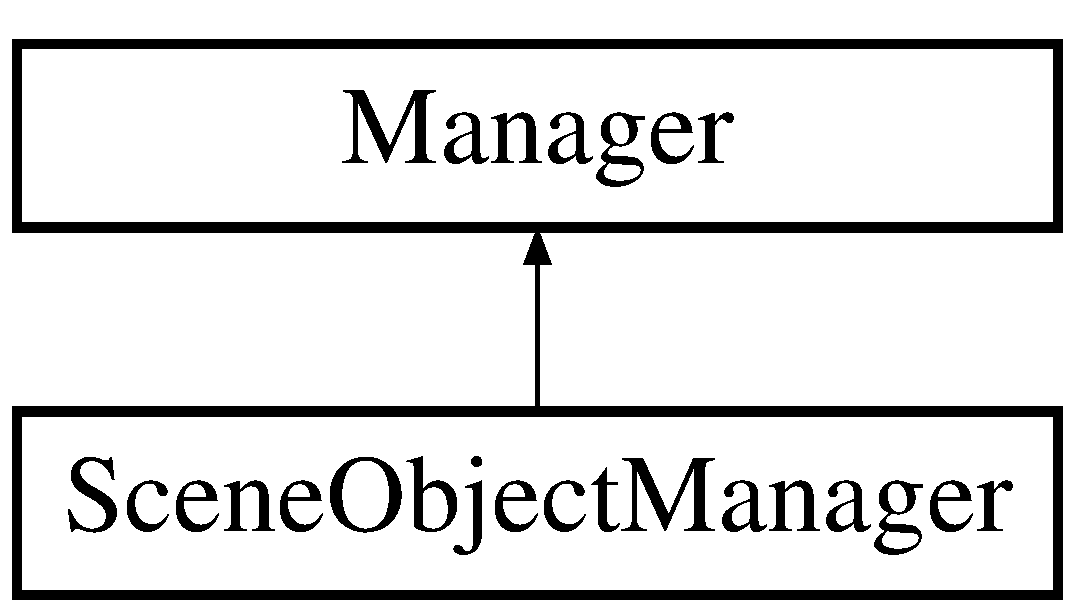
\includegraphics[height=2.000000cm]{class_scene_object_manager}
\end{center}
\end{figure}
\subsection*{Public Member Functions}
\begin{DoxyCompactItemize}
\item 
\hyperlink{class_scene_object_manager_a589afc363b4e3f7d04f253c43205763a}{Scene\+Object\+Manager} ()
\begin{DoxyCompactList}\small\item\em Default constructor. \end{DoxyCompactList}\item 
\hyperlink{class_scene_object_manager_adffb8c511196411d515c9b230b85c8e5}{$\sim$\+Scene\+Object\+Manager} ()
\begin{DoxyCompactList}\small\item\em Default destructor. \end{DoxyCompactList}\item 
void \hyperlink{class_scene_object_manager_a4231d373cedd650cd5a6ee7930f76994}{add\+Scene\+Object} (std\+::shared\+\_\+ptr$<$ \hyperlink{class_scene_object}{Scene\+Object} $>$ object)
\begin{DoxyCompactList}\small\item\em Add a scene object to the scene. \end{DoxyCompactList}\item 
void \hyperlink{class_scene_object_manager_a00b65df9f837802b33150a51e3315278}{remove\+Scene\+Object} (std\+::shared\+\_\+ptr$<$ \hyperlink{class_scene_object}{Scene\+Object} $>$ object)
\begin{DoxyCompactList}\small\item\em Remove a scene object from the scene (and destroy if applicable) \end{DoxyCompactList}\item 
void \hyperlink{class_scene_object_manager_ae760816e4028cc680dce44dde42ced52}{get\+Objects} (std\+::list$<$ std\+::shared\+\_\+ptr$<$ \hyperlink{class_scene_object}{Scene\+Object} $>$$>$ $\ast$objects)
\begin{DoxyCompactList}\small\item\em Retrieve the list of objects in the scene. \end{DoxyCompactList}\item 
void \hyperlink{class_scene_object_manager_a95eb6fa59723180a1ced2775249a0afe}{step} (double dt)
\begin{DoxyCompactList}\small\item\em Step the scene\textquotesingle{}s simulation state. \end{DoxyCompactList}\item 
void \hyperlink{class_scene_object_manager_a895153bc766085c9f94e4be72733b807}{predraw} (\hyperlink{class_context}{Context} $\ast$context)
\begin{DoxyCompactList}\small\item\em Called before the renderer draws the scene This allows the scene and its constituent objects to do updates that require a graphics context before the graphical state is drawn. \end{DoxyCompactList}\end{DoxyCompactItemize}
\subsection*{Private Member Functions}
\begin{DoxyCompactItemize}
\item 
void \hyperlink{class_scene_object_manager_a09f307f2c9fde4b85995f62fc21f731a}{cleanup\+Dying\+Objects} ()
\begin{DoxyCompactList}\small\item\em Finalize the death and cleanup of objects marked as dying. \end{DoxyCompactList}\end{DoxyCompactItemize}
\subsection*{Private Attributes}
\begin{DoxyCompactItemize}
\item 
std\+::list$<$ std\+::shared\+\_\+ptr$<$ \hyperlink{class_scene_object}{Scene\+Object} $>$ $>$ \hyperlink{class_scene_object_manager_a3fec371160b895369edb7c694e205050}{m\+\_\+\+Scene\+Objects}
\end{DoxyCompactItemize}


\subsection{Detailed Description}
A manager class for handling and passing around scene objects. 

\begin{DoxyAuthor}{Author}
Hayley Hatton 
\end{DoxyAuthor}
\begin{DoxyDate}{Date}
11/03/2016 
\end{DoxyDate}


Definition at line 13 of file Scene\+Object\+Manager.\+h.



\subsection{Constructor \& Destructor Documentation}
\index{Scene\+Object\+Manager@{Scene\+Object\+Manager}!Scene\+Object\+Manager@{Scene\+Object\+Manager}}
\index{Scene\+Object\+Manager@{Scene\+Object\+Manager}!Scene\+Object\+Manager@{Scene\+Object\+Manager}}
\subsubsection[{\texorpdfstring{Scene\+Object\+Manager()}{SceneObjectManager()}}]{\setlength{\rightskip}{0pt plus 5cm}Scene\+Object\+Manager\+::\+Scene\+Object\+Manager (
\begin{DoxyParamCaption}
{}
\end{DoxyParamCaption}
)}\hypertarget{class_scene_object_manager_a589afc363b4e3f7d04f253c43205763a}{}\label{class_scene_object_manager_a589afc363b4e3f7d04f253c43205763a}


Default constructor. 



Definition at line 4 of file Scene\+Object\+Manager.\+cpp.

\index{Scene\+Object\+Manager@{Scene\+Object\+Manager}!````~Scene\+Object\+Manager@{$\sim$\+Scene\+Object\+Manager}}
\index{````~Scene\+Object\+Manager@{$\sim$\+Scene\+Object\+Manager}!Scene\+Object\+Manager@{Scene\+Object\+Manager}}
\subsubsection[{\texorpdfstring{$\sim$\+Scene\+Object\+Manager()}{~SceneObjectManager()}}]{\setlength{\rightskip}{0pt plus 5cm}Scene\+Object\+Manager\+::$\sim$\+Scene\+Object\+Manager (
\begin{DoxyParamCaption}
{}
\end{DoxyParamCaption}
)}\hypertarget{class_scene_object_manager_adffb8c511196411d515c9b230b85c8e5}{}\label{class_scene_object_manager_adffb8c511196411d515c9b230b85c8e5}


Default destructor. 



Definition at line 8 of file Scene\+Object\+Manager.\+cpp.



\subsection{Member Function Documentation}
\index{Scene\+Object\+Manager@{Scene\+Object\+Manager}!add\+Scene\+Object@{add\+Scene\+Object}}
\index{add\+Scene\+Object@{add\+Scene\+Object}!Scene\+Object\+Manager@{Scene\+Object\+Manager}}
\subsubsection[{\texorpdfstring{add\+Scene\+Object(std\+::shared\+\_\+ptr$<$ Scene\+Object $>$ object)}{addSceneObject(std::shared_ptr< SceneObject > object)}}]{\setlength{\rightskip}{0pt plus 5cm}void Scene\+Object\+Manager\+::add\+Scene\+Object (
\begin{DoxyParamCaption}
\item[{std\+::shared\+\_\+ptr$<$ {\bf Scene\+Object} $>$}]{object}
\end{DoxyParamCaption}
)}\hypertarget{class_scene_object_manager_a4231d373cedd650cd5a6ee7930f76994}{}\label{class_scene_object_manager_a4231d373cedd650cd5a6ee7930f76994}


Add a scene object to the scene. 


\begin{DoxyParams}{Parameters}
{\em object} & Smart ptr to the scene object \\
\hline
\end{DoxyParams}


Definition at line 13 of file Scene\+Object\+Manager.\+cpp.



References m\+\_\+\+Scene\+Objects.



Referenced by Scene\+::add\+Object().

\index{Scene\+Object\+Manager@{Scene\+Object\+Manager}!cleanup\+Dying\+Objects@{cleanup\+Dying\+Objects}}
\index{cleanup\+Dying\+Objects@{cleanup\+Dying\+Objects}!Scene\+Object\+Manager@{Scene\+Object\+Manager}}
\subsubsection[{\texorpdfstring{cleanup\+Dying\+Objects()}{cleanupDyingObjects()}}]{\setlength{\rightskip}{0pt plus 5cm}void Scene\+Object\+Manager\+::cleanup\+Dying\+Objects (
\begin{DoxyParamCaption}
{}
\end{DoxyParamCaption}
)\hspace{0.3cm}{\ttfamily [private]}}\hypertarget{class_scene_object_manager_a09f307f2c9fde4b85995f62fc21f731a}{}\label{class_scene_object_manager_a09f307f2c9fde4b85995f62fc21f731a}


Finalize the death and cleanup of objects marked as dying. 



Definition at line 41 of file Scene\+Object\+Manager.\+cpp.



References Scene\+Object\+::\+Dying, and m\+\_\+\+Scene\+Objects.



Referenced by predraw().

\index{Scene\+Object\+Manager@{Scene\+Object\+Manager}!get\+Objects@{get\+Objects}}
\index{get\+Objects@{get\+Objects}!Scene\+Object\+Manager@{Scene\+Object\+Manager}}
\subsubsection[{\texorpdfstring{get\+Objects(std\+::list$<$ std\+::shared\+\_\+ptr$<$ Scene\+Object $>$$>$ $\ast$objects)}{getObjects(std::list< std::shared_ptr< SceneObject >> *objects)}}]{\setlength{\rightskip}{0pt plus 5cm}void Scene\+Object\+Manager\+::get\+Objects (
\begin{DoxyParamCaption}
\item[{std\+::list$<$ std\+::shared\+\_\+ptr$<$ {\bf Scene\+Object} $>$$>$ $\ast$}]{objects}
\end{DoxyParamCaption}
)}\hypertarget{class_scene_object_manager_ae760816e4028cc680dce44dde42ced52}{}\label{class_scene_object_manager_ae760816e4028cc680dce44dde42ced52}


Retrieve the list of objects in the scene. 


\begin{DoxyParams}{Parameters}
{\em objects} & Pointer to list to fill with scene objects \\
\hline
\end{DoxyParams}


Definition at line 25 of file Scene\+Object\+Manager.\+cpp.



References m\+\_\+\+Scene\+Objects.



Referenced by Scene\+::get\+Objects().

\index{Scene\+Object\+Manager@{Scene\+Object\+Manager}!predraw@{predraw}}
\index{predraw@{predraw}!Scene\+Object\+Manager@{Scene\+Object\+Manager}}
\subsubsection[{\texorpdfstring{predraw(\+Context $\ast$context)}{predraw(Context *context)}}]{\setlength{\rightskip}{0pt plus 5cm}void Scene\+Object\+Manager\+::predraw (
\begin{DoxyParamCaption}
\item[{{\bf Context} $\ast$}]{context}
\end{DoxyParamCaption}
)}\hypertarget{class_scene_object_manager_a895153bc766085c9f94e4be72733b807}{}\label{class_scene_object_manager_a895153bc766085c9f94e4be72733b807}


Called before the renderer draws the scene This allows the scene and its constituent objects to do updates that require a graphics context before the graphical state is drawn. 


\begin{DoxyParams}{Parameters}
{\em context} & Graphics context \\
\hline
\end{DoxyParams}


Definition at line 57 of file Scene\+Object\+Manager.\+cpp.



References cleanup\+Dying\+Objects(), m\+\_\+\+Scene\+Objects, and Scene\+Object\+::\+Ready.



Referenced by Scene\+::predraw().

\index{Scene\+Object\+Manager@{Scene\+Object\+Manager}!remove\+Scene\+Object@{remove\+Scene\+Object}}
\index{remove\+Scene\+Object@{remove\+Scene\+Object}!Scene\+Object\+Manager@{Scene\+Object\+Manager}}
\subsubsection[{\texorpdfstring{remove\+Scene\+Object(std\+::shared\+\_\+ptr$<$ Scene\+Object $>$ object)}{removeSceneObject(std::shared_ptr< SceneObject > object)}}]{\setlength{\rightskip}{0pt plus 5cm}void Scene\+Object\+Manager\+::remove\+Scene\+Object (
\begin{DoxyParamCaption}
\item[{std\+::shared\+\_\+ptr$<$ {\bf Scene\+Object} $>$}]{object}
\end{DoxyParamCaption}
)}\hypertarget{class_scene_object_manager_a00b65df9f837802b33150a51e3315278}{}\label{class_scene_object_manager_a00b65df9f837802b33150a51e3315278}


Remove a scene object from the scene (and destroy if applicable) 


\begin{DoxyParams}{Parameters}
{\em object} & Smart ptr to the scene object to remove \\
\hline
\end{DoxyParams}


Definition at line 19 of file Scene\+Object\+Manager.\+cpp.



References m\+\_\+\+Scene\+Objects.

\index{Scene\+Object\+Manager@{Scene\+Object\+Manager}!step@{step}}
\index{step@{step}!Scene\+Object\+Manager@{Scene\+Object\+Manager}}
\subsubsection[{\texorpdfstring{step(double dt)}{step(double dt)}}]{\setlength{\rightskip}{0pt plus 5cm}void Scene\+Object\+Manager\+::step (
\begin{DoxyParamCaption}
\item[{double}]{dt}
\end{DoxyParamCaption}
)}\hypertarget{class_scene_object_manager_a95eb6fa59723180a1ced2775249a0afe}{}\label{class_scene_object_manager_a95eb6fa59723180a1ced2775249a0afe}


Step the scene\textquotesingle{}s simulation state. 


\begin{DoxyParams}{Parameters}
{\em dt} & Delta-\/time since last step call in seconds \\
\hline
\end{DoxyParams}


Definition at line 31 of file Scene\+Object\+Manager.\+cpp.



References m\+\_\+\+Scene\+Objects.



Referenced by Scene\+::step().



\subsection{Member Data Documentation}
\index{Scene\+Object\+Manager@{Scene\+Object\+Manager}!m\+\_\+\+Scene\+Objects@{m\+\_\+\+Scene\+Objects}}
\index{m\+\_\+\+Scene\+Objects@{m\+\_\+\+Scene\+Objects}!Scene\+Object\+Manager@{Scene\+Object\+Manager}}
\subsubsection[{\texorpdfstring{m\+\_\+\+Scene\+Objects}{m_SceneObjects}}]{\setlength{\rightskip}{0pt plus 5cm}std\+::list$<$std\+::shared\+\_\+ptr$<${\bf Scene\+Object}$>$ $>$ Scene\+Object\+Manager\+::m\+\_\+\+Scene\+Objects\hspace{0.3cm}{\ttfamily [private]}}\hypertarget{class_scene_object_manager_a3fec371160b895369edb7c694e205050}{}\label{class_scene_object_manager_a3fec371160b895369edb7c694e205050}


Definition at line 56 of file Scene\+Object\+Manager.\+h.



Referenced by add\+Scene\+Object(), cleanup\+Dying\+Objects(), get\+Objects(), predraw(), remove\+Scene\+Object(), and step().



The documentation for this class was generated from the following files\+:\begin{DoxyCompactItemize}
\item 
Lunar\+Drift/engine/managers/\hyperlink{_scene_object_manager_8h}{Scene\+Object\+Manager.\+h}\item 
Lunar\+Drift/engine/managers/\hyperlink{_scene_object_manager_8cpp}{Scene\+Object\+Manager.\+cpp}\end{DoxyCompactItemize}

\hypertarget{class_shader_exception}{}\section{Shader\+Exception Class Reference}
\label{class_shader_exception}\index{Shader\+Exception@{Shader\+Exception}}


Exception raised whenever a shader operation fails.  




{\ttfamily \#include $<$Shader\+Exception.\+h$>$}

Inheritance diagram for Shader\+Exception\+:\begin{figure}[H]
\begin{center}
\leavevmode
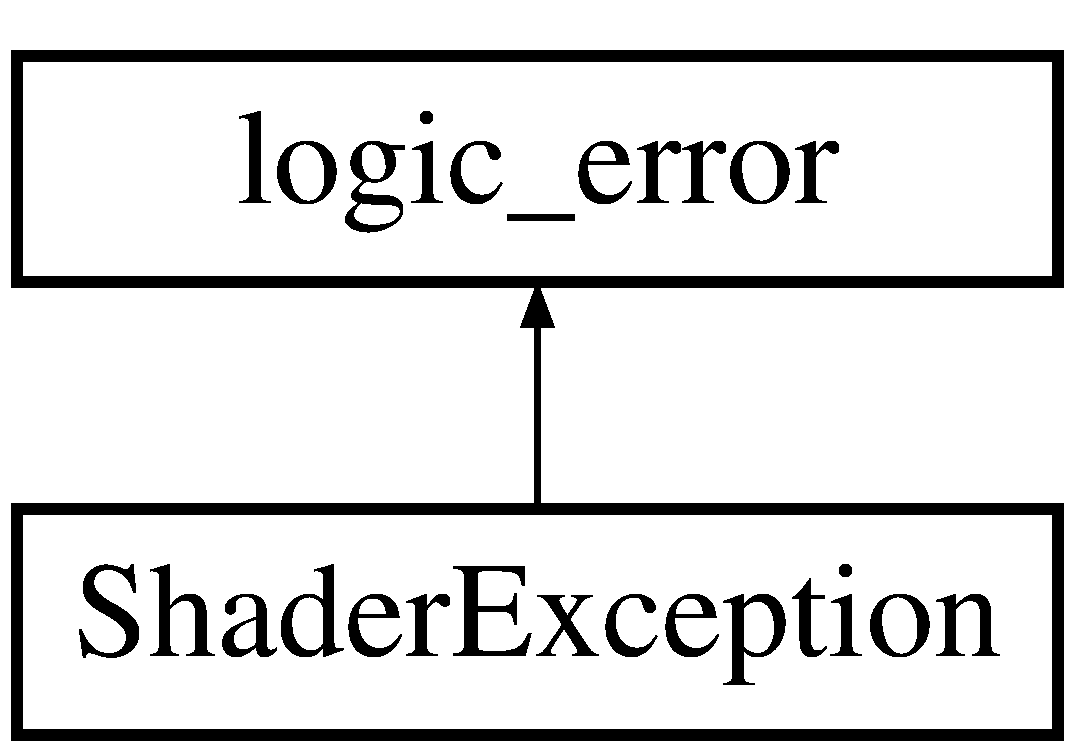
\includegraphics[height=2.000000cm]{class_shader_exception}
\end{center}
\end{figure}
\subsection*{Public Member Functions}
\begin{DoxyCompactItemize}
\item 
\hyperlink{class_shader_exception_a049037e52e22d2a229def811ca6713fd}{Shader\+Exception} (const std\+::string \&file, const std\+::string \&component, const std\+::string \&stage, const std\+::string \&error\+Log)
\begin{DoxyCompactList}\small\item\em Default constructor. \end{DoxyCompactList}\item 
const std\+::string \& \hyperlink{class_shader_exception_a1e3806a87d7707f9da52095d8f4de530}{get\+File} () const 
\item 
const std\+::string \& \hyperlink{class_shader_exception_a634ea552b39aa510aef3436df9c5c95d}{get\+Component} () const 
\item 
const std\+::string \& \hyperlink{class_shader_exception_a855c9f2b9363c2ce6f2439b4b44a2380}{get\+Stage} () const 
\item 
const std\+::string \& \hyperlink{class_shader_exception_a34911ad17ca116d95d41c45f4faccc7c}{get\+Error\+Log} () const 
\end{DoxyCompactItemize}
\subsection*{Private Attributes}
\begin{DoxyCompactItemize}
\item 
const std\+::string \hyperlink{class_shader_exception_a0f130003946a31fb9f79258f5b2978c6}{m\+\_\+\+File}
\item 
const std\+::string \hyperlink{class_shader_exception_aa87a250d03b97c4080d3e287fbda9dd1}{m\+\_\+\+Component}
\item 
const std\+::string \hyperlink{class_shader_exception_aa6b0663a6cca810a07367f21f77a9c43}{m\+\_\+\+Stage}
\item 
const std\+::string \hyperlink{class_shader_exception_ad8b59e0d8c6bda3add539cb0386579d2}{m\+\_\+\+Error\+Log}
\end{DoxyCompactItemize}


\subsection{Detailed Description}
Exception raised whenever a shader operation fails. 

\begin{DoxyAuthor}{Author}
Hayley Hatton 
\end{DoxyAuthor}
\begin{DoxyDate}{Date}
20/02/2016 
\end{DoxyDate}


Definition at line 12 of file Shader\+Exception.\+h.



\subsection{Constructor \& Destructor Documentation}
\index{Shader\+Exception@{Shader\+Exception}!Shader\+Exception@{Shader\+Exception}}
\index{Shader\+Exception@{Shader\+Exception}!Shader\+Exception@{Shader\+Exception}}
\subsubsection[{\texorpdfstring{Shader\+Exception(const std\+::string \&file, const std\+::string \&component, const std\+::string \&stage, const std\+::string \&error\+Log)}{ShaderException(const std::string &file, const std::string &component, const std::string &stage, const std::string &errorLog)}}]{\setlength{\rightskip}{0pt plus 5cm}Shader\+Exception\+::\+Shader\+Exception (
\begin{DoxyParamCaption}
\item[{const std\+::string \&}]{file, }
\item[{const std\+::string \&}]{component, }
\item[{const std\+::string \&}]{stage, }
\item[{const std\+::string \&}]{error\+Log}
\end{DoxyParamCaption}
)}\hypertarget{class_shader_exception_a049037e52e22d2a229def811ca6713fd}{}\label{class_shader_exception_a049037e52e22d2a229def811ca6713fd}


Default constructor. 


\begin{DoxyParams}{Parameters}
{\em file} & File where the error was raised \\
\hline
{\em component} & Shader component of the program where it went wrong \\
\hline
{\em stage} & Stage of the shader pipeline where the error was raised \\
\hline
{\em error\+Log} & Generated error log \\
\hline
\end{DoxyParams}


Definition at line 3 of file Shader\+Exception.\+cpp.



\subsection{Member Function Documentation}
\index{Shader\+Exception@{Shader\+Exception}!get\+Component@{get\+Component}}
\index{get\+Component@{get\+Component}!Shader\+Exception@{Shader\+Exception}}
\subsubsection[{\texorpdfstring{get\+Component() const }{getComponent() const }}]{\setlength{\rightskip}{0pt plus 5cm}const std\+::string\& Shader\+Exception\+::get\+Component (
\begin{DoxyParamCaption}
{}
\end{DoxyParamCaption}
) const\hspace{0.3cm}{\ttfamily [inline]}}\hypertarget{class_shader_exception_a634ea552b39aa510aef3436df9c5c95d}{}\label{class_shader_exception_a634ea552b39aa510aef3436df9c5c95d}


Definition at line 31 of file Shader\+Exception.\+h.



References m\+\_\+\+Component.



Referenced by Window\+P\+C\+::rendering\+Thread(), and Win\+Main().

\index{Shader\+Exception@{Shader\+Exception}!get\+Error\+Log@{get\+Error\+Log}}
\index{get\+Error\+Log@{get\+Error\+Log}!Shader\+Exception@{Shader\+Exception}}
\subsubsection[{\texorpdfstring{get\+Error\+Log() const }{getErrorLog() const }}]{\setlength{\rightskip}{0pt plus 5cm}const std\+::string\& Shader\+Exception\+::get\+Error\+Log (
\begin{DoxyParamCaption}
{}
\end{DoxyParamCaption}
) const\hspace{0.3cm}{\ttfamily [inline]}}\hypertarget{class_shader_exception_a34911ad17ca116d95d41c45f4faccc7c}{}\label{class_shader_exception_a34911ad17ca116d95d41c45f4faccc7c}


Definition at line 35 of file Shader\+Exception.\+h.



References m\+\_\+\+Error\+Log.



Referenced by Window\+P\+C\+::rendering\+Thread(), and Win\+Main().

\index{Shader\+Exception@{Shader\+Exception}!get\+File@{get\+File}}
\index{get\+File@{get\+File}!Shader\+Exception@{Shader\+Exception}}
\subsubsection[{\texorpdfstring{get\+File() const }{getFile() const }}]{\setlength{\rightskip}{0pt plus 5cm}const std\+::string\& Shader\+Exception\+::get\+File (
\begin{DoxyParamCaption}
{}
\end{DoxyParamCaption}
) const\hspace{0.3cm}{\ttfamily [inline]}}\hypertarget{class_shader_exception_a1e3806a87d7707f9da52095d8f4de530}{}\label{class_shader_exception_a1e3806a87d7707f9da52095d8f4de530}


Definition at line 29 of file Shader\+Exception.\+h.



References m\+\_\+\+File.



Referenced by Window\+P\+C\+::rendering\+Thread(), and Win\+Main().

\index{Shader\+Exception@{Shader\+Exception}!get\+Stage@{get\+Stage}}
\index{get\+Stage@{get\+Stage}!Shader\+Exception@{Shader\+Exception}}
\subsubsection[{\texorpdfstring{get\+Stage() const }{getStage() const }}]{\setlength{\rightskip}{0pt plus 5cm}const std\+::string\& Shader\+Exception\+::get\+Stage (
\begin{DoxyParamCaption}
{}
\end{DoxyParamCaption}
) const\hspace{0.3cm}{\ttfamily [inline]}}\hypertarget{class_shader_exception_a855c9f2b9363c2ce6f2439b4b44a2380}{}\label{class_shader_exception_a855c9f2b9363c2ce6f2439b4b44a2380}


Definition at line 33 of file Shader\+Exception.\+h.



References m\+\_\+\+Stage.



Referenced by Window\+P\+C\+::rendering\+Thread(), and Win\+Main().



\subsection{Member Data Documentation}
\index{Shader\+Exception@{Shader\+Exception}!m\+\_\+\+Component@{m\+\_\+\+Component}}
\index{m\+\_\+\+Component@{m\+\_\+\+Component}!Shader\+Exception@{Shader\+Exception}}
\subsubsection[{\texorpdfstring{m\+\_\+\+Component}{m_Component}}]{\setlength{\rightskip}{0pt plus 5cm}const std\+::string Shader\+Exception\+::m\+\_\+\+Component\hspace{0.3cm}{\ttfamily [private]}}\hypertarget{class_shader_exception_aa87a250d03b97c4080d3e287fbda9dd1}{}\label{class_shader_exception_aa87a250d03b97c4080d3e287fbda9dd1}


Definition at line 40 of file Shader\+Exception.\+h.



Referenced by get\+Component().

\index{Shader\+Exception@{Shader\+Exception}!m\+\_\+\+Error\+Log@{m\+\_\+\+Error\+Log}}
\index{m\+\_\+\+Error\+Log@{m\+\_\+\+Error\+Log}!Shader\+Exception@{Shader\+Exception}}
\subsubsection[{\texorpdfstring{m\+\_\+\+Error\+Log}{m_ErrorLog}}]{\setlength{\rightskip}{0pt plus 5cm}const std\+::string Shader\+Exception\+::m\+\_\+\+Error\+Log\hspace{0.3cm}{\ttfamily [private]}}\hypertarget{class_shader_exception_ad8b59e0d8c6bda3add539cb0386579d2}{}\label{class_shader_exception_ad8b59e0d8c6bda3add539cb0386579d2}


Definition at line 42 of file Shader\+Exception.\+h.



Referenced by get\+Error\+Log().

\index{Shader\+Exception@{Shader\+Exception}!m\+\_\+\+File@{m\+\_\+\+File}}
\index{m\+\_\+\+File@{m\+\_\+\+File}!Shader\+Exception@{Shader\+Exception}}
\subsubsection[{\texorpdfstring{m\+\_\+\+File}{m_File}}]{\setlength{\rightskip}{0pt plus 5cm}const std\+::string Shader\+Exception\+::m\+\_\+\+File\hspace{0.3cm}{\ttfamily [private]}}\hypertarget{class_shader_exception_a0f130003946a31fb9f79258f5b2978c6}{}\label{class_shader_exception_a0f130003946a31fb9f79258f5b2978c6}


Definition at line 39 of file Shader\+Exception.\+h.



Referenced by get\+File().

\index{Shader\+Exception@{Shader\+Exception}!m\+\_\+\+Stage@{m\+\_\+\+Stage}}
\index{m\+\_\+\+Stage@{m\+\_\+\+Stage}!Shader\+Exception@{Shader\+Exception}}
\subsubsection[{\texorpdfstring{m\+\_\+\+Stage}{m_Stage}}]{\setlength{\rightskip}{0pt plus 5cm}const std\+::string Shader\+Exception\+::m\+\_\+\+Stage\hspace{0.3cm}{\ttfamily [private]}}\hypertarget{class_shader_exception_aa6b0663a6cca810a07367f21f77a9c43}{}\label{class_shader_exception_aa6b0663a6cca810a07367f21f77a9c43}


Definition at line 41 of file Shader\+Exception.\+h.



Referenced by get\+Stage().



The documentation for this class was generated from the following files\+:\begin{DoxyCompactItemize}
\item 
Lunar\+Drift/engine/exceptions/\hyperlink{_shader_exception_8h}{Shader\+Exception.\+h}\item 
Lunar\+Drift/engine/exceptions/\hyperlink{_shader_exception_8cpp}{Shader\+Exception.\+cpp}\end{DoxyCompactItemize}

\hypertarget{class_shader_manager}{}\section{Shader\+Manager Class Reference}
\label{class_shader_manager}\index{Shader\+Manager@{Shader\+Manager}}


Container for associating shader programs with shading class key names.  




{\ttfamily \#include $<$Shader\+Manager.\+h$>$}

\subsection*{Public Member Functions}
\begin{DoxyCompactItemize}
\item 
\hyperlink{class_shader_manager_aca25f81fd10a02b3e97e9c459b864186}{Shader\+Manager} ()
\begin{DoxyCompactList}\small\item\em Default constructor. \end{DoxyCompactList}\item 
virtual \hyperlink{class_shader_manager_a7603399f16432b94223b9fa78f74fb87}{$\sim$\+Shader\+Manager} ()
\begin{DoxyCompactList}\small\item\em Default destructor. \end{DoxyCompactList}\item 
void \hyperlink{class_shader_manager_a9a39a329a279db43c84fce10fee9a706}{set} (const std\+::string \&key, std\+::shared\+\_\+ptr$<$ \hyperlink{class_shader_program}{Shader\+Program} $>$ shader)
\begin{DoxyCompactList}\small\item\em Associate a shader program with a shading class key. \end{DoxyCompactList}\item 
std\+::shared\+\_\+ptr$<$ \hyperlink{class_shader_program}{Shader\+Program} $>$ \hyperlink{class_shader_manager_a42a3df3ac4d2bce3153fff3d967fd97f}{get} (const std\+::string \&key)
\begin{DoxyCompactList}\small\item\em Return an associated shader program from a given shading class. \end{DoxyCompactList}\item 
void \hyperlink{class_shader_manager_a8288a4814f4a4fd228262ea3bef18673}{get} (std\+::vector$<$ std\+::shared\+\_\+ptr$<$ \hyperlink{class_shader_program}{Shader\+Program} $>$$>$ $\ast$shaders) const 
\begin{DoxyCompactList}\small\item\em Get a list of all the shader programs in the manager. \end{DoxyCompactList}\end{DoxyCompactItemize}
\subsection*{Private Attributes}
\begin{DoxyCompactItemize}
\item 
std\+::map$<$ std\+::string, std\+::shared\+\_\+ptr$<$ \hyperlink{class_shader_program}{Shader\+Program} $>$ $>$ \hyperlink{class_shader_manager_a8b3bab142565af9177794f380db932e7}{m\+\_\+\+Shader\+Map}
\end{DoxyCompactItemize}


\subsection{Detailed Description}
Container for associating shader programs with shading class key names. 

This class thus encapsulates shader management away from the renderers, and allows a map of shader programs associated with shading classes to be passed around easily.

\begin{DoxyAuthor}{Author}
Hayley Hatton 
\end{DoxyAuthor}
\begin{DoxyDate}{Date}
07/03/2016 
\end{DoxyDate}
\begin{DoxySeeAlso}{See also}
\hyperlink{class_shader_program}{Shader\+Program} 

\hyperlink{class_renderer}{Renderer} 
\end{DoxySeeAlso}


Definition at line 19 of file Shader\+Manager.\+h.



\subsection{Constructor \& Destructor Documentation}
\index{Shader\+Manager@{Shader\+Manager}!Shader\+Manager@{Shader\+Manager}}
\index{Shader\+Manager@{Shader\+Manager}!Shader\+Manager@{Shader\+Manager}}
\subsubsection[{\texorpdfstring{Shader\+Manager()}{ShaderManager()}}]{\setlength{\rightskip}{0pt plus 5cm}Shader\+Manager\+::\+Shader\+Manager (
\begin{DoxyParamCaption}
{}
\end{DoxyParamCaption}
)}\hypertarget{class_shader_manager_aca25f81fd10a02b3e97e9c459b864186}{}\label{class_shader_manager_aca25f81fd10a02b3e97e9c459b864186}


Default constructor. 



Definition at line 4 of file Shader\+Manager.\+cpp.

\index{Shader\+Manager@{Shader\+Manager}!````~Shader\+Manager@{$\sim$\+Shader\+Manager}}
\index{````~Shader\+Manager@{$\sim$\+Shader\+Manager}!Shader\+Manager@{Shader\+Manager}}
\subsubsection[{\texorpdfstring{$\sim$\+Shader\+Manager()}{~ShaderManager()}}]{\setlength{\rightskip}{0pt plus 5cm}Shader\+Manager\+::$\sim$\+Shader\+Manager (
\begin{DoxyParamCaption}
{}
\end{DoxyParamCaption}
)\hspace{0.3cm}{\ttfamily [virtual]}}\hypertarget{class_shader_manager_a7603399f16432b94223b9fa78f74fb87}{}\label{class_shader_manager_a7603399f16432b94223b9fa78f74fb87}


Default destructor. 



Definition at line 9 of file Shader\+Manager.\+cpp.



\subsection{Member Function Documentation}
\index{Shader\+Manager@{Shader\+Manager}!get@{get}}
\index{get@{get}!Shader\+Manager@{Shader\+Manager}}
\subsubsection[{\texorpdfstring{get(const std\+::string \&key)}{get(const std::string &key)}}]{\setlength{\rightskip}{0pt plus 5cm}std\+::shared\+\_\+ptr$<$ {\bf Shader\+Program} $>$ Shader\+Manager\+::get (
\begin{DoxyParamCaption}
\item[{const std\+::string \&}]{key}
\end{DoxyParamCaption}
)}\hypertarget{class_shader_manager_a42a3df3ac4d2bce3153fff3d967fd97f}{}\label{class_shader_manager_a42a3df3ac4d2bce3153fff3d967fd97f}


Return an associated shader program from a given shading class. 


\begin{DoxyParams}{Parameters}
{\em key} & Shading class name \\
\hline
\end{DoxyParams}
\begin{DoxyReturn}{Returns}
Associated shader program 
\end{DoxyReturn}


Definition at line 22 of file Shader\+Manager.\+cpp.



References m\+\_\+\+Shader\+Map.

\index{Shader\+Manager@{Shader\+Manager}!get@{get}}
\index{get@{get}!Shader\+Manager@{Shader\+Manager}}
\subsubsection[{\texorpdfstring{get(std\+::vector$<$ std\+::shared\+\_\+ptr$<$ Shader\+Program $>$$>$ $\ast$shaders) const }{get(std::vector< std::shared_ptr< ShaderProgram >> *shaders) const }}]{\setlength{\rightskip}{0pt plus 5cm}void Shader\+Manager\+::get (
\begin{DoxyParamCaption}
\item[{std\+::vector$<$ std\+::shared\+\_\+ptr$<$ {\bf Shader\+Program} $>$$>$ $\ast$}]{shaders}
\end{DoxyParamCaption}
) const}\hypertarget{class_shader_manager_a8288a4814f4a4fd228262ea3bef18673}{}\label{class_shader_manager_a8288a4814f4a4fd228262ea3bef18673}


Get a list of all the shader programs in the manager. 


\begin{DoxyParams}{Parameters}
{\em shaders} & Pointer to a vector class to hold the shader programs \\
\hline
\end{DoxyParams}


Definition at line 30 of file Shader\+Manager.\+cpp.



References m\+\_\+\+Shader\+Map.

\index{Shader\+Manager@{Shader\+Manager}!set@{set}}
\index{set@{set}!Shader\+Manager@{Shader\+Manager}}
\subsubsection[{\texorpdfstring{set(const std\+::string \&key, std\+::shared\+\_\+ptr$<$ Shader\+Program $>$ shader)}{set(const std::string &key, std::shared_ptr< ShaderProgram > shader)}}]{\setlength{\rightskip}{0pt plus 5cm}void Shader\+Manager\+::set (
\begin{DoxyParamCaption}
\item[{const std\+::string \&}]{key, }
\item[{std\+::shared\+\_\+ptr$<$ {\bf Shader\+Program} $>$}]{shader}
\end{DoxyParamCaption}
)}\hypertarget{class_shader_manager_a9a39a329a279db43c84fce10fee9a706}{}\label{class_shader_manager_a9a39a329a279db43c84fce10fee9a706}


Associate a shader program with a shading class key. 


\begin{DoxyParams}{Parameters}
{\em key} & Shading class name \\
\hline
{\em shader} & Shader program to associate \\
\hline
\end{DoxyParams}


Definition at line 15 of file Shader\+Manager.\+cpp.



References m\+\_\+\+Shader\+Map.



\subsection{Member Data Documentation}
\index{Shader\+Manager@{Shader\+Manager}!m\+\_\+\+Shader\+Map@{m\+\_\+\+Shader\+Map}}
\index{m\+\_\+\+Shader\+Map@{m\+\_\+\+Shader\+Map}!Shader\+Manager@{Shader\+Manager}}
\subsubsection[{\texorpdfstring{m\+\_\+\+Shader\+Map}{m_ShaderMap}}]{\setlength{\rightskip}{0pt plus 5cm}std\+::map$<$std\+::string,std\+::shared\+\_\+ptr$<${\bf Shader\+Program}$>$ $>$ Shader\+Manager\+::m\+\_\+\+Shader\+Map\hspace{0.3cm}{\ttfamily [private]}}\hypertarget{class_shader_manager_a8b3bab142565af9177794f380db932e7}{}\label{class_shader_manager_a8b3bab142565af9177794f380db932e7}


Definition at line 50 of file Shader\+Manager.\+h.



Referenced by get(), and set().



The documentation for this class was generated from the following files\+:\begin{DoxyCompactItemize}
\item 
Lunar\+Drift/engine/managers/\hyperlink{_shader_manager_8h}{Shader\+Manager.\+h}\item 
Lunar\+Drift/engine/managers/\hyperlink{_shader_manager_8cpp}{Shader\+Manager.\+cpp}\end{DoxyCompactItemize}

\hypertarget{class_shader_program}{}\section{Shader\+Program Class Reference}
\label{class_shader_program}\index{Shader\+Program@{Shader\+Program}}


Container for a G\+L\+SL shader program and its constituent shaders.  




{\ttfamily \#include $<$Shader\+Program.\+h$>$}

\subsection*{Public Member Functions}
\begin{DoxyCompactItemize}
\item 
\hyperlink{class_shader_program_a4cc1af7c22b52019885503fb16e5c837}{Shader\+Program} (const std\+::string \&vertex, const std\+::string \&fragment)
\begin{DoxyCompactList}\small\item\em Normal shader program constructor. \end{DoxyCompactList}\item 
\hyperlink{class_shader_program_af16e52eb0d138a14e33902b7ec313a6b}{Shader\+Program} (const std\+::string \&vertex, const std\+::string \&geometry, const std\+::string \&fragment)
\begin{DoxyCompactList}\small\item\em Shader program w/ geometry shader constructor. \end{DoxyCompactList}\item 
virtual \hyperlink{class_shader_program_a2d2eadcfc48cc2e2ddb82aba70553a9f}{$\sim$\+Shader\+Program} ()
\begin{DoxyCompactList}\small\item\em Default destructor. \end{DoxyCompactList}\item 
void \hyperlink{class_shader_program_a2231dc8ed81e75d4f36260b90cb19f4a}{load} (const std\+::string \&vertex, const std\+::string \&fragment)
\begin{DoxyCompactList}\small\item\em Loads a shader program (Open\+GL 2 required) \end{DoxyCompactList}\item 
void \hyperlink{class_shader_program_a69a116f12f5f9fcf8c7b4f97c15bb2da}{load} (const std\+::string \&vertex, const std\+::string \&geometry, const std\+::string \&fragment)
\begin{DoxyCompactList}\small\item\em Loads a shader program (Open\+GL 3.\+2 required) \end{DoxyCompactList}\item 
void \hyperlink{class_shader_program_a45ba12614fbdc743632baa677edd2247}{unload} ()
\begin{DoxyCompactList}\small\item\em Unloads the shader program and its children. \end{DoxyCompactList}\item 
G\+Luint \hyperlink{class_shader_program_a90f0b84a857b82aa1220246e9aeed9bd}{get\+Program\+Handle} () const 
\begin{DoxyCompactList}\small\item\em Returns the program handle of the shader program. \end{DoxyCompactList}\item 
G\+Lint \hyperlink{class_shader_program_aba49891be3e62c2fa03f3e0f03abd7df}{get\+Attribute\+Location} (const std\+::string \&name) const 
\begin{DoxyCompactList}\small\item\em Obtains the location of an attribute in the shader program. \end{DoxyCompactList}\item 
G\+Lint \hyperlink{class_shader_program_a434f4f504303d9132c5b8b89126d8c08}{get\+Uniform\+Location} (const std\+::string \&name) const 
\begin{DoxyCompactList}\small\item\em Obtains the location of a uniform in the shader program. \end{DoxyCompactList}\item 
int \hyperlink{class_shader_program_a771afbb9e66163c6ac685eb16d690ba0}{get\+Uniform\+Block\+Location} (const std\+::string \&name) const 
\begin{DoxyCompactList}\small\item\em Get the identifier of a given uniform block. \end{DoxyCompactList}\item 
void \hyperlink{class_shader_program_a753715c1bcc5c718f15c29ccb09a7261}{bind\+Uniform\+Block} (const std\+::string \&name, int binding\+Point) const 
\begin{DoxyCompactList}\small\item\em Bind a given uniform block at an index. \end{DoxyCompactList}\item 
void \hyperlink{class_shader_program_ad9fef410acc1d6246ea32fa4e5b48b8a}{use} (\hyperlink{class_context}{Context} $\ast$context)
\begin{DoxyCompactList}\small\item\em Bind the shader program to the Open\+GL state pipeline. \end{DoxyCompactList}\end{DoxyCompactItemize}
\subsection*{Protected Member Functions}
\begin{DoxyCompactItemize}
\item 
G\+Lint \hyperlink{class_shader_program_a0dd6ee69d550a6826129ce3a0b227e93}{load\+And\+Compile\+File} (const std\+::string \&name, G\+Lenum stage)
\begin{DoxyCompactList}\small\item\em Load and compile shader code from a file. \end{DoxyCompactList}\item 
void \hyperlink{class_shader_program_a402c1d0936a1feb9b4981f747beaab59}{read\+Shader\+File} (const std\+::string \&filename, std\+::string $\ast$data)
\begin{DoxyCompactList}\small\item\em Reads a shader from a file and returns its source code. \end{DoxyCompactList}\end{DoxyCompactItemize}
\subsection*{Private Attributes}
{\bf }\par
\begin{DoxyCompactItemize}
\item 
G\+Luint \hyperlink{class_shader_program_aeeb7c9dabeaae9aba49858cf3221d887}{m\+\_\+\+Program\+Handle}
\begin{DoxyCompactList}\small\item\em Shader handlers. \end{DoxyCompactList}\item 
G\+Lint \hyperlink{class_shader_program_a2056277d1b0c3a71a7b783e17e3733a1}{m\+\_\+\+Vertex\+Shader\+Handle}
\item 
G\+Lint \hyperlink{class_shader_program_ac9959fc7ce96370c40c1422e7d104a44}{m\+\_\+\+Geometry\+Shader\+Handle}
\item 
G\+Lint \hyperlink{class_shader_program_a8fe8505db597cb168b538df824d03906}{m\+\_\+\+Fragment\+Shader\+Handle}
\end{DoxyCompactItemize}



\subsection{Detailed Description}
Container for a G\+L\+SL shader program and its constituent shaders. 

This is composed of two to three shaders (if using geometry shaders) compiled and linked into a \char`\"{}shader program\char`\"{}.

This supports Vertex/\+Fragment Shaders and Vertex/\+Geometry/\+Fragment Shaders. Version 4 is not supported, and so Tessellation Control and Evaluator shaders are available.

\begin{DoxyPrecond}{Precondition}
A valid Open\+GL context must be present to the program. 
\end{DoxyPrecond}
\begin{DoxyAuthor}{Author}
Hayley Hatton 
\end{DoxyAuthor}
\begin{DoxyDate}{Date}
06/03/2016 
\end{DoxyDate}


Definition at line 20 of file Shader\+Program.\+h.



\subsection{Constructor \& Destructor Documentation}
\index{Shader\+Program@{Shader\+Program}!Shader\+Program@{Shader\+Program}}
\index{Shader\+Program@{Shader\+Program}!Shader\+Program@{Shader\+Program}}
\subsubsection[{\texorpdfstring{Shader\+Program(const std\+::string \&vertex, const std\+::string \&fragment)}{ShaderProgram(const std::string &vertex, const std::string &fragment)}}]{\setlength{\rightskip}{0pt plus 5cm}Shader\+Program\+::\+Shader\+Program (
\begin{DoxyParamCaption}
\item[{const std\+::string \&}]{vertex, }
\item[{const std\+::string \&}]{fragment}
\end{DoxyParamCaption}
)}\hypertarget{class_shader_program_a4cc1af7c22b52019885503fb16e5c837}{}\label{class_shader_program_a4cc1af7c22b52019885503fb16e5c837}


Normal shader program constructor. 


\begin{DoxyParams}{Parameters}
{\em vertex} & Vertex shader filename, minus .vert extension \\
\hline
{\em fragment} & Fragment shader filename, minus .frag extension \\
\hline
\end{DoxyParams}

\begin{DoxyExceptions}{Exceptions}
{\em \hyperlink{class_file_i_o_exception}{File\+I\+O\+Exception}} & \\
\hline
{\em Shader\+Compile\+Exception} & \\
\hline
{\em \hyperlink{class_open_g_l_exception}{Open\+G\+L\+Exception}} & \\
\hline
\end{DoxyExceptions}


Definition at line 9 of file Shader\+Program.\+cpp.



References load().

\index{Shader\+Program@{Shader\+Program}!Shader\+Program@{Shader\+Program}}
\index{Shader\+Program@{Shader\+Program}!Shader\+Program@{Shader\+Program}}
\subsubsection[{\texorpdfstring{Shader\+Program(const std\+::string \&vertex, const std\+::string \&geometry, const std\+::string \&fragment)}{ShaderProgram(const std::string &vertex, const std::string &geometry, const std::string &fragment)}}]{\setlength{\rightskip}{0pt plus 5cm}Shader\+Program\+::\+Shader\+Program (
\begin{DoxyParamCaption}
\item[{const std\+::string \&}]{vertex, }
\item[{const std\+::string \&}]{geometry, }
\item[{const std\+::string \&}]{fragment}
\end{DoxyParamCaption}
)}\hypertarget{class_shader_program_af16e52eb0d138a14e33902b7ec313a6b}{}\label{class_shader_program_af16e52eb0d138a14e33902b7ec313a6b}


Shader program w/ geometry shader constructor. 


\begin{DoxyParams}{Parameters}
{\em vertex} & Vertex shader filename, minus .vert extension \\
\hline
{\em geometry} & Geometry shader filename \\
\hline
{\em fragment} & Fragment shader filename, minus .frag extension \\
\hline
\end{DoxyParams}

\begin{DoxyExceptions}{Exceptions}
{\em \hyperlink{class_file_i_o_exception}{File\+I\+O\+Exception}} & \\
\hline
{\em Shader\+Compile\+Exception} & \\
\hline
{\em \hyperlink{class_open_g_l_exception}{Open\+G\+L\+Exception}} & \\
\hline
\end{DoxyExceptions}


Definition at line 16 of file Shader\+Program.\+cpp.



References load().

\index{Shader\+Program@{Shader\+Program}!````~Shader\+Program@{$\sim$\+Shader\+Program}}
\index{````~Shader\+Program@{$\sim$\+Shader\+Program}!Shader\+Program@{Shader\+Program}}
\subsubsection[{\texorpdfstring{$\sim$\+Shader\+Program()}{~ShaderProgram()}}]{\setlength{\rightskip}{0pt plus 5cm}Shader\+Program\+::$\sim$\+Shader\+Program (
\begin{DoxyParamCaption}
{}
\end{DoxyParamCaption}
)\hspace{0.3cm}{\ttfamily [virtual]}}\hypertarget{class_shader_program_a2d2eadcfc48cc2e2ddb82aba70553a9f}{}\label{class_shader_program_a2d2eadcfc48cc2e2ddb82aba70553a9f}


Default destructor. 



Definition at line 24 of file Shader\+Program.\+cpp.



References unload().



\subsection{Member Function Documentation}
\index{Shader\+Program@{Shader\+Program}!bind\+Uniform\+Block@{bind\+Uniform\+Block}}
\index{bind\+Uniform\+Block@{bind\+Uniform\+Block}!Shader\+Program@{Shader\+Program}}
\subsubsection[{\texorpdfstring{bind\+Uniform\+Block(const std\+::string \&name, int binding\+Point) const }{bindUniformBlock(const std::string &name, int bindingPoint) const }}]{\setlength{\rightskip}{0pt plus 5cm}void Shader\+Program\+::bind\+Uniform\+Block (
\begin{DoxyParamCaption}
\item[{const std\+::string \&}]{name, }
\item[{int}]{binding\+Point}
\end{DoxyParamCaption}
) const\hspace{0.3cm}{\ttfamily [inline]}}\hypertarget{class_shader_program_a753715c1bcc5c718f15c29ccb09a7261}{}\label{class_shader_program_a753715c1bcc5c718f15c29ccb09a7261}


Bind a given uniform block at an index. 


\begin{DoxyParams}{Parameters}
{\em name} & Name of the uniform block \\
\hline
\end{DoxyParams}
\begin{DoxyReturn}{Returns}
Index to bind the uniform block at 
\end{DoxyReturn}


Definition at line 123 of file Shader\+Program.\+h.



References m\+\_\+\+Program\+Handle.

\index{Shader\+Program@{Shader\+Program}!get\+Attribute\+Location@{get\+Attribute\+Location}}
\index{get\+Attribute\+Location@{get\+Attribute\+Location}!Shader\+Program@{Shader\+Program}}
\subsubsection[{\texorpdfstring{get\+Attribute\+Location(const std\+::string \&name) const }{getAttributeLocation(const std::string &name) const }}]{\setlength{\rightskip}{0pt plus 5cm}G\+Lint Shader\+Program\+::get\+Attribute\+Location (
\begin{DoxyParamCaption}
\item[{const std\+::string \&}]{name}
\end{DoxyParamCaption}
) const\hspace{0.3cm}{\ttfamily [inline]}}\hypertarget{class_shader_program_aba49891be3e62c2fa03f3e0f03abd7df}{}\label{class_shader_program_aba49891be3e62c2fa03f3e0f03abd7df}


Obtains the location of an attribute in the shader program. 


\begin{DoxyParams}{Parameters}
{\em name} & Name of the attribute \\
\hline
\end{DoxyParams}
\begin{DoxyReturn}{Returns}
Handle to the attribute; -\/1 if error 
\end{DoxyReturn}


Definition at line 96 of file Shader\+Program.\+h.



References m\+\_\+\+Program\+Handle.

\index{Shader\+Program@{Shader\+Program}!get\+Program\+Handle@{get\+Program\+Handle}}
\index{get\+Program\+Handle@{get\+Program\+Handle}!Shader\+Program@{Shader\+Program}}
\subsubsection[{\texorpdfstring{get\+Program\+Handle() const }{getProgramHandle() const }}]{\setlength{\rightskip}{0pt plus 5cm}G\+Luint Shader\+Program\+::get\+Program\+Handle (
\begin{DoxyParamCaption}
{}
\end{DoxyParamCaption}
) const\hspace{0.3cm}{\ttfamily [inline]}}\hypertarget{class_shader_program_a90f0b84a857b82aa1220246e9aeed9bd}{}\label{class_shader_program_a90f0b84a857b82aa1220246e9aeed9bd}


Returns the program handle of the shader program. 

\begin{DoxyReturn}{Returns}
\hyperlink{class_program}{Program} handle 
\end{DoxyReturn}


Definition at line 89 of file Shader\+Program.\+h.



References m\+\_\+\+Program\+Handle.

\index{Shader\+Program@{Shader\+Program}!get\+Uniform\+Block\+Location@{get\+Uniform\+Block\+Location}}
\index{get\+Uniform\+Block\+Location@{get\+Uniform\+Block\+Location}!Shader\+Program@{Shader\+Program}}
\subsubsection[{\texorpdfstring{get\+Uniform\+Block\+Location(const std\+::string \&name) const }{getUniformBlockLocation(const std::string &name) const }}]{\setlength{\rightskip}{0pt plus 5cm}int Shader\+Program\+::get\+Uniform\+Block\+Location (
\begin{DoxyParamCaption}
\item[{const std\+::string \&}]{name}
\end{DoxyParamCaption}
) const\hspace{0.3cm}{\ttfamily [inline]}}\hypertarget{class_shader_program_a771afbb9e66163c6ac685eb16d690ba0}{}\label{class_shader_program_a771afbb9e66163c6ac685eb16d690ba0}


Get the identifier of a given uniform block. 


\begin{DoxyParams}{Parameters}
{\em name} & Name of the uniform block \\
\hline
\end{DoxyParams}
\begin{DoxyReturn}{Returns}
Identifier of the uniform block 
\end{DoxyReturn}


Definition at line 114 of file Shader\+Program.\+h.



References m\+\_\+\+Program\+Handle.

\index{Shader\+Program@{Shader\+Program}!get\+Uniform\+Location@{get\+Uniform\+Location}}
\index{get\+Uniform\+Location@{get\+Uniform\+Location}!Shader\+Program@{Shader\+Program}}
\subsubsection[{\texorpdfstring{get\+Uniform\+Location(const std\+::string \&name) const }{getUniformLocation(const std::string &name) const }}]{\setlength{\rightskip}{0pt plus 5cm}G\+Lint Shader\+Program\+::get\+Uniform\+Location (
\begin{DoxyParamCaption}
\item[{const std\+::string \&}]{name}
\end{DoxyParamCaption}
) const\hspace{0.3cm}{\ttfamily [inline]}}\hypertarget{class_shader_program_a434f4f504303d9132c5b8b89126d8c08}{}\label{class_shader_program_a434f4f504303d9132c5b8b89126d8c08}


Obtains the location of a uniform in the shader program. 


\begin{DoxyParams}{Parameters}
{\em name} & Name of the uniform \\
\hline
\end{DoxyParams}
\begin{DoxyReturn}{Returns}
Handle to the uniform; -\/1 if error 
\end{DoxyReturn}


Definition at line 105 of file Shader\+Program.\+h.



References m\+\_\+\+Program\+Handle.



Referenced by Camera\+::apply().

\index{Shader\+Program@{Shader\+Program}!load@{load}}
\index{load@{load}!Shader\+Program@{Shader\+Program}}
\subsubsection[{\texorpdfstring{load(const std\+::string \&vertex, const std\+::string \&fragment)}{load(const std::string &vertex, const std::string &fragment)}}]{\setlength{\rightskip}{0pt plus 5cm}void Shader\+Program\+::load (
\begin{DoxyParamCaption}
\item[{const std\+::string \&}]{vertex, }
\item[{const std\+::string \&}]{fragment}
\end{DoxyParamCaption}
)}\hypertarget{class_shader_program_a2231dc8ed81e75d4f36260b90cb19f4a}{}\label{class_shader_program_a2231dc8ed81e75d4f36260b90cb19f4a}


Loads a shader program (Open\+GL 2 required) 


\begin{DoxyParams}{Parameters}
{\em vertex} & Vertex shader filename, minus .vert extension \\
\hline
{\em fragment} & Fragment shader filename, minus .frag extension \\
\hline
\end{DoxyParams}

\begin{DoxyExceptions}{Exceptions}
{\em \hyperlink{class_file_i_o_exception}{File\+I\+O\+Exception}} & \\
\hline
{\em Shader\+Compile\+Exception} & \\
\hline
{\em \hyperlink{class_open_g_l_exception}{Open\+G\+L\+Exception}} & \\
\hline
\end{DoxyExceptions}


Definition at line 29 of file Shader\+Program.\+cpp.



References load\+And\+Compile\+File(), m\+\_\+\+Fragment\+Shader\+Handle, m\+\_\+\+Geometry\+Shader\+Handle, m\+\_\+\+Program\+Handle, and m\+\_\+\+Vertex\+Shader\+Handle.



Referenced by Shader\+Program().

\index{Shader\+Program@{Shader\+Program}!load@{load}}
\index{load@{load}!Shader\+Program@{Shader\+Program}}
\subsubsection[{\texorpdfstring{load(const std\+::string \&vertex, const std\+::string \&geometry, const std\+::string \&fragment)}{load(const std::string &vertex, const std::string &geometry, const std::string &fragment)}}]{\setlength{\rightskip}{0pt plus 5cm}void Shader\+Program\+::load (
\begin{DoxyParamCaption}
\item[{const std\+::string \&}]{vertex, }
\item[{const std\+::string \&}]{geometry, }
\item[{const std\+::string \&}]{fragment}
\end{DoxyParamCaption}
)}\hypertarget{class_shader_program_a69a116f12f5f9fcf8c7b4f97c15bb2da}{}\label{class_shader_program_a69a116f12f5f9fcf8c7b4f97c15bb2da}


Loads a shader program (Open\+GL 3.\+2 required) 


\begin{DoxyParams}{Parameters}
{\em vertex} & Vertex shader filename, minus .vert extension \\
\hline
{\em geometry} & Geometry shader filename, minus .geom extension \\
\hline
{\em fragment} & Fragment shader filename, minus .frag extension \\
\hline
\end{DoxyParams}

\begin{DoxyExceptions}{Exceptions}
{\em \hyperlink{class_file_i_o_exception}{File\+I\+O\+Exception}} & \\
\hline
{\em Shader\+Compile\+Exception} & \\
\hline
{\em \hyperlink{class_open_g_l_exception}{Open\+G\+L\+Exception}} & \\
\hline
\end{DoxyExceptions}


Definition at line 73 of file Shader\+Program.\+cpp.



References load\+And\+Compile\+File(), m\+\_\+\+Fragment\+Shader\+Handle, m\+\_\+\+Geometry\+Shader\+Handle, m\+\_\+\+Program\+Handle, and m\+\_\+\+Vertex\+Shader\+Handle.

\index{Shader\+Program@{Shader\+Program}!load\+And\+Compile\+File@{load\+And\+Compile\+File}}
\index{load\+And\+Compile\+File@{load\+And\+Compile\+File}!Shader\+Program@{Shader\+Program}}
\subsubsection[{\texorpdfstring{load\+And\+Compile\+File(const std\+::string \&name, G\+Lenum stage)}{loadAndCompileFile(const std::string &name, GLenum stage)}}]{\setlength{\rightskip}{0pt plus 5cm}G\+Lint Shader\+Program\+::load\+And\+Compile\+File (
\begin{DoxyParamCaption}
\item[{const std\+::string \&}]{name, }
\item[{G\+Lenum}]{stage}
\end{DoxyParamCaption}
)\hspace{0.3cm}{\ttfamily [protected]}}\hypertarget{class_shader_program_a0dd6ee69d550a6826129ce3a0b227e93}{}\label{class_shader_program_a0dd6ee69d550a6826129ce3a0b227e93}


Load and compile shader code from a file. 


\begin{DoxyParams}{Parameters}
{\em name} & Shader filename \\
\hline
{\em stage} & Shader stage (e.\+g. G\+L\+\_\+\+V\+E\+R\+T\+E\+X\+\_\+\+S\+H\+A\+D\+ER) \\
\hline
\end{DoxyParams}
\begin{DoxyReturn}{Returns}
Handle to the shader code on the G\+PU 
\end{DoxyReturn}

\begin{DoxyExceptions}{Exceptions}
{\em \hyperlink{class_file_i_o_exception}{File\+I\+O\+Exception}} & \\
\hline
{\em Shader\+Compile\+Exception} & \\
\hline
\end{DoxyExceptions}


Definition at line 121 of file Shader\+Program.\+cpp.



References read\+Shader\+File().



Referenced by load(), and use().

\index{Shader\+Program@{Shader\+Program}!read\+Shader\+File@{read\+Shader\+File}}
\index{read\+Shader\+File@{read\+Shader\+File}!Shader\+Program@{Shader\+Program}}
\subsubsection[{\texorpdfstring{read\+Shader\+File(const std\+::string \&filename, std\+::string $\ast$data)}{readShaderFile(const std::string &filename, std::string *data)}}]{\setlength{\rightskip}{0pt plus 5cm}void Shader\+Program\+::read\+Shader\+File (
\begin{DoxyParamCaption}
\item[{const std\+::string \&}]{filename, }
\item[{std\+::string $\ast$}]{data}
\end{DoxyParamCaption}
)\hspace{0.3cm}{\ttfamily [protected]}}\hypertarget{class_shader_program_a402c1d0936a1feb9b4981f747beaab59}{}\label{class_shader_program_a402c1d0936a1feb9b4981f747beaab59}


Reads a shader from a file and returns its source code. 


\begin{DoxyParams}{Parameters}
{\em filename} & Location of the shader file \\
\hline
{\em data} & Ptr to string to be filled with the shader file\textquotesingle{}s data \\
\hline
\end{DoxyParams}

\begin{DoxyExceptions}{Exceptions}
{\em \hyperlink{class_file_i_o_exception}{File\+I\+O\+Exception}} & \\
\hline
\end{DoxyExceptions}


Definition at line 183 of file Shader\+Program.\+cpp.



References Config\+::get().



Referenced by load\+And\+Compile\+File(), and use().

\index{Shader\+Program@{Shader\+Program}!unload@{unload}}
\index{unload@{unload}!Shader\+Program@{Shader\+Program}}
\subsubsection[{\texorpdfstring{unload()}{unload()}}]{\setlength{\rightskip}{0pt plus 5cm}void Shader\+Program\+::unload (
\begin{DoxyParamCaption}
{}
\end{DoxyParamCaption}
)}\hypertarget{class_shader_program_a45ba12614fbdc743632baa677edd2247}{}\label{class_shader_program_a45ba12614fbdc743632baa677edd2247}


Unloads the shader program and its children. 



Definition at line 174 of file Shader\+Program.\+cpp.



References m\+\_\+\+Fragment\+Shader\+Handle, m\+\_\+\+Geometry\+Shader\+Handle, m\+\_\+\+Program\+Handle, and m\+\_\+\+Vertex\+Shader\+Handle.



Referenced by $\sim$\+Shader\+Program().

\index{Shader\+Program@{Shader\+Program}!use@{use}}
\index{use@{use}!Shader\+Program@{Shader\+Program}}
\subsubsection[{\texorpdfstring{use(\+Context $\ast$context)}{use(Context *context)}}]{\setlength{\rightskip}{0pt plus 5cm}void Shader\+Program\+::use (
\begin{DoxyParamCaption}
\item[{{\bf Context} $\ast$}]{context}
\end{DoxyParamCaption}
)\hspace{0.3cm}{\ttfamily [inline]}}\hypertarget{class_shader_program_ad9fef410acc1d6246ea32fa4e5b48b8a}{}\label{class_shader_program_ad9fef410acc1d6246ea32fa4e5b48b8a}


Bind the shader program to the Open\+GL state pipeline. 



Definition at line 131 of file Shader\+Program.\+h.



References load\+And\+Compile\+File(), m\+\_\+\+Program\+Handle, and read\+Shader\+File().



Referenced by Camera\+::apply().



\subsection{Member Data Documentation}
\index{Shader\+Program@{Shader\+Program}!m\+\_\+\+Fragment\+Shader\+Handle@{m\+\_\+\+Fragment\+Shader\+Handle}}
\index{m\+\_\+\+Fragment\+Shader\+Handle@{m\+\_\+\+Fragment\+Shader\+Handle}!Shader\+Program@{Shader\+Program}}
\subsubsection[{\texorpdfstring{m\+\_\+\+Fragment\+Shader\+Handle}{m_FragmentShaderHandle}}]{\setlength{\rightskip}{0pt plus 5cm}G\+Lint Shader\+Program\+::m\+\_\+\+Fragment\+Shader\+Handle\hspace{0.3cm}{\ttfamily [private]}}\hypertarget{class_shader_program_a8fe8505db597cb168b538df824d03906}{}\label{class_shader_program_a8fe8505db597cb168b538df824d03906}


Definition at line 159 of file Shader\+Program.\+h.



Referenced by load(), and unload().

\index{Shader\+Program@{Shader\+Program}!m\+\_\+\+Geometry\+Shader\+Handle@{m\+\_\+\+Geometry\+Shader\+Handle}}
\index{m\+\_\+\+Geometry\+Shader\+Handle@{m\+\_\+\+Geometry\+Shader\+Handle}!Shader\+Program@{Shader\+Program}}
\subsubsection[{\texorpdfstring{m\+\_\+\+Geometry\+Shader\+Handle}{m_GeometryShaderHandle}}]{\setlength{\rightskip}{0pt plus 5cm}G\+Lint Shader\+Program\+::m\+\_\+\+Geometry\+Shader\+Handle\hspace{0.3cm}{\ttfamily [private]}}\hypertarget{class_shader_program_ac9959fc7ce96370c40c1422e7d104a44}{}\label{class_shader_program_ac9959fc7ce96370c40c1422e7d104a44}


Definition at line 158 of file Shader\+Program.\+h.



Referenced by load(), and unload().

\index{Shader\+Program@{Shader\+Program}!m\+\_\+\+Program\+Handle@{m\+\_\+\+Program\+Handle}}
\index{m\+\_\+\+Program\+Handle@{m\+\_\+\+Program\+Handle}!Shader\+Program@{Shader\+Program}}
\subsubsection[{\texorpdfstring{m\+\_\+\+Program\+Handle}{m_ProgramHandle}}]{\setlength{\rightskip}{0pt plus 5cm}G\+Luint Shader\+Program\+::m\+\_\+\+Program\+Handle\hspace{0.3cm}{\ttfamily [private]}}\hypertarget{class_shader_program_aeeb7c9dabeaae9aba49858cf3221d887}{}\label{class_shader_program_aeeb7c9dabeaae9aba49858cf3221d887}


Shader handlers. 



Definition at line 156 of file Shader\+Program.\+h.



Referenced by bind\+Uniform\+Block(), get\+Attribute\+Location(), get\+Program\+Handle(), get\+Uniform\+Block\+Location(), get\+Uniform\+Location(), load(), unload(), and use().

\index{Shader\+Program@{Shader\+Program}!m\+\_\+\+Vertex\+Shader\+Handle@{m\+\_\+\+Vertex\+Shader\+Handle}}
\index{m\+\_\+\+Vertex\+Shader\+Handle@{m\+\_\+\+Vertex\+Shader\+Handle}!Shader\+Program@{Shader\+Program}}
\subsubsection[{\texorpdfstring{m\+\_\+\+Vertex\+Shader\+Handle}{m_VertexShaderHandle}}]{\setlength{\rightskip}{0pt plus 5cm}G\+Lint Shader\+Program\+::m\+\_\+\+Vertex\+Shader\+Handle\hspace{0.3cm}{\ttfamily [private]}}\hypertarget{class_shader_program_a2056277d1b0c3a71a7b783e17e3733a1}{}\label{class_shader_program_a2056277d1b0c3a71a7b783e17e3733a1}


Definition at line 157 of file Shader\+Program.\+h.



Referenced by load(), and unload().



The documentation for this class was generated from the following files\+:\begin{DoxyCompactItemize}
\item 
Lunar\+Drift/engine/graphics/shaders/\hyperlink{_shader_program_8h}{Shader\+Program.\+h}\item 
Lunar\+Drift/engine/graphics/shaders/\hyperlink{_shader_program_8cpp}{Shader\+Program.\+cpp}\end{DoxyCompactItemize}

\hypertarget{class_shader_uniform_block}{}\section{Shader\+Uniform\+Block Class Reference}
\label{class_shader_uniform_block}\index{Shader\+Uniform\+Block@{Shader\+Uniform\+Block}}


{\ttfamily \#include $<$Shader\+Uniform\+Block.\+h$>$}

\subsection*{Public Member Functions}
\begin{DoxyCompactItemize}
\item 
\hyperlink{class_shader_uniform_block_a6239ead8f4fb7965d65550173f62dca9}{Shader\+Uniform\+Block} ()
\item 
virtual \hyperlink{class_shader_uniform_block_ab4b157c5a69cfad3389f0aa4270efe3c}{$\sim$\+Shader\+Uniform\+Block} ()
\end{DoxyCompactItemize}


\subsection{Detailed Description}


Definition at line 3 of file Shader\+Uniform\+Block.\+h.



\subsection{Constructor \& Destructor Documentation}
\index{Shader\+Uniform\+Block@{Shader\+Uniform\+Block}!Shader\+Uniform\+Block@{Shader\+Uniform\+Block}}
\index{Shader\+Uniform\+Block@{Shader\+Uniform\+Block}!Shader\+Uniform\+Block@{Shader\+Uniform\+Block}}
\subsubsection[{\texorpdfstring{Shader\+Uniform\+Block()}{ShaderUniformBlock()}}]{\setlength{\rightskip}{0pt plus 5cm}Shader\+Uniform\+Block\+::\+Shader\+Uniform\+Block (
\begin{DoxyParamCaption}
{}
\end{DoxyParamCaption}
)}\hypertarget{class_shader_uniform_block_a6239ead8f4fb7965d65550173f62dca9}{}\label{class_shader_uniform_block_a6239ead8f4fb7965d65550173f62dca9}
Default constructor 

Definition at line 3 of file Shader\+Uniform\+Block.\+cpp.

\index{Shader\+Uniform\+Block@{Shader\+Uniform\+Block}!````~Shader\+Uniform\+Block@{$\sim$\+Shader\+Uniform\+Block}}
\index{````~Shader\+Uniform\+Block@{$\sim$\+Shader\+Uniform\+Block}!Shader\+Uniform\+Block@{Shader\+Uniform\+Block}}
\subsubsection[{\texorpdfstring{$\sim$\+Shader\+Uniform\+Block()}{~ShaderUniformBlock()}}]{\setlength{\rightskip}{0pt plus 5cm}Shader\+Uniform\+Block\+::$\sim$\+Shader\+Uniform\+Block (
\begin{DoxyParamCaption}
{}
\end{DoxyParamCaption}
)\hspace{0.3cm}{\ttfamily [virtual]}}\hypertarget{class_shader_uniform_block_ab4b157c5a69cfad3389f0aa4270efe3c}{}\label{class_shader_uniform_block_ab4b157c5a69cfad3389f0aa4270efe3c}
Default destructor 

Definition at line 8 of file Shader\+Uniform\+Block.\+cpp.



The documentation for this class was generated from the following files\+:\begin{DoxyCompactItemize}
\item 
Lunar\+Drift/engine/graphics/shaders/\hyperlink{_shader_uniform_block_8h}{Shader\+Uniform\+Block.\+h}\item 
Lunar\+Drift/engine/graphics/shaders/\hyperlink{_shader_uniform_block_8cpp}{Shader\+Uniform\+Block.\+cpp}\end{DoxyCompactItemize}

\hypertarget{class_test_scene3_d}{}\section{Test\+Scene3D Class Reference}
\label{class_test_scene3_d}\index{Test\+Scene3D@{Test\+Scene3D}}


{\ttfamily \#include $<$Test\+Scene3\+D.\+h$>$}

Inheritance diagram for Test\+Scene3D\+:\begin{figure}[H]
\begin{center}
\leavevmode
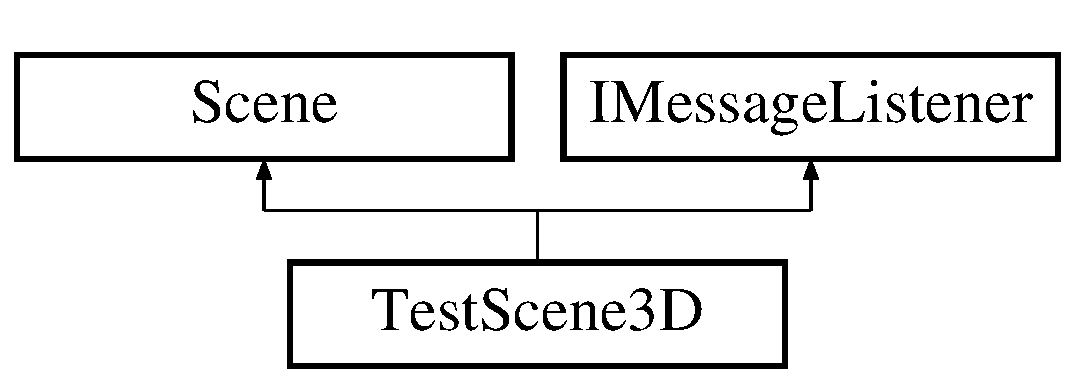
\includegraphics[height=2.000000cm]{class_test_scene3_d}
\end{center}
\end{figure}
\subsection*{Public Member Functions}
\begin{DoxyCompactItemize}
\item 
\hyperlink{class_test_scene3_d_a0e6437d4668fbb54f7d62d408e0a99ea}{Test\+Scene3D} (\hyperlink{class_context}{Context} $\ast$context)
\begin{DoxyCompactList}\small\item\em Default constructor. \end{DoxyCompactList}\item 
virtual \hyperlink{class_test_scene3_d_a912bd9b4b8561d3ed9caab3ad42d2693}{$\sim$\+Test\+Scene3D} ()
\begin{DoxyCompactList}\small\item\em Default destructor. \end{DoxyCompactList}\item 
void \hyperlink{class_test_scene3_d_ab762c0baa39e323b598f08945d50bb1f}{set\+Size} (G\+Lsizei width, G\+Lsizei height) override
\begin{DoxyCompactList}\small\item\em Called to update scene elements with the viewport information. \end{DoxyCompactList}\item 
void \hyperlink{class_test_scene3_d_aebf275cd7c567dca7d8662ff859d2acf}{step} (double dt) override
\begin{DoxyCompactList}\small\item\em Step the scene\textquotesingle{}s simulation state. \end{DoxyCompactList}\item 
void \hyperlink{class_test_scene3_d_ab87089331bf0fb71d09361624dc1c53e}{predraw} (\hyperlink{class_context}{Context} $\ast$context) override
\begin{DoxyCompactList}\small\item\em Called before the renderer draws the scene This allows the scene and its constituent objects to do updates that require a graphics context before the graphical state is drawn. \end{DoxyCompactList}\item 
void \hyperlink{class_test_scene3_d_aa5c6527ffc929e51eb3303431bfc6f7d}{on\+Message} (std\+::shared\+\_\+ptr$<$ \hyperlink{class_message}{Message} $>$ event) override
\begin{DoxyCompactList}\small\item\em Called when a subscribed event is raised. \end{DoxyCompactList}\end{DoxyCompactItemize}
\subsection*{Private Attributes}
\begin{DoxyCompactItemize}
\item 
G\+Lfloat \hyperlink{class_test_scene3_d_ad645a73819745449c00db8b800417565}{m\+\_\+\+Distance}
\item 
G\+Lfloat \hyperlink{class_test_scene3_d_ac4a67a6b4358d147b417c4dcf9735ad4}{m\+\_\+\+Offset}
\end{DoxyCompactItemize}
\subsection*{Additional Inherited Members}


\subsection{Detailed Description}


Definition at line 6 of file Test\+Scene3\+D.\+h.



\subsection{Constructor \& Destructor Documentation}
\index{Test\+Scene3D@{Test\+Scene3D}!Test\+Scene3D@{Test\+Scene3D}}
\index{Test\+Scene3D@{Test\+Scene3D}!Test\+Scene3D@{Test\+Scene3D}}
\subsubsection[{\texorpdfstring{Test\+Scene3\+D(\+Context $\ast$context)}{TestScene3D(Context *context)}}]{\setlength{\rightskip}{0pt plus 5cm}Test\+Scene3\+D\+::\+Test\+Scene3D (
\begin{DoxyParamCaption}
\item[{{\bf Context} $\ast$}]{context}
\end{DoxyParamCaption}
)}\hypertarget{class_test_scene3_d_a0e6437d4668fbb54f7d62d408e0a99ea}{}\label{class_test_scene3_d_a0e6437d4668fbb54f7d62d408e0a99ea}


Default constructor. 


\begin{DoxyParams}{Parameters}
{\em context} & Graphics context \\
\hline
\end{DoxyParams}


Definition at line 8 of file Test\+Scene3\+D.\+cpp.



References Scene\+::add\+Object(), f, Config\+::get(), Context\+::get\+Dimensions(), Config\+::get\+Float(), Message\+System\+::get\+Instance(), Scene\+::get\+Managers(), m\+\_\+\+Distance, Scene\+::set\+Active\+Camera(), and Message\+System\+::subscribe().

\index{Test\+Scene3D@{Test\+Scene3D}!````~Test\+Scene3D@{$\sim$\+Test\+Scene3D}}
\index{````~Test\+Scene3D@{$\sim$\+Test\+Scene3D}!Test\+Scene3D@{Test\+Scene3D}}
\subsubsection[{\texorpdfstring{$\sim$\+Test\+Scene3\+D()}{~TestScene3D()}}]{\setlength{\rightskip}{0pt plus 5cm}Test\+Scene3\+D\+::$\sim$\+Test\+Scene3D (
\begin{DoxyParamCaption}
{}
\end{DoxyParamCaption}
)\hspace{0.3cm}{\ttfamily [virtual]}}\hypertarget{class_test_scene3_d_a912bd9b4b8561d3ed9caab3ad42d2693}{}\label{class_test_scene3_d_a912bd9b4b8561d3ed9caab3ad42d2693}


Default destructor. 



Definition at line 32 of file Test\+Scene3\+D.\+cpp.



\subsection{Member Function Documentation}
\index{Test\+Scene3D@{Test\+Scene3D}!on\+Message@{on\+Message}}
\index{on\+Message@{on\+Message}!Test\+Scene3D@{Test\+Scene3D}}
\subsubsection[{\texorpdfstring{on\+Message(std\+::shared\+\_\+ptr$<$ Message $>$ event) override}{onMessage(std::shared_ptr< Message > event) override}}]{\setlength{\rightskip}{0pt plus 5cm}void Test\+Scene3\+D\+::on\+Message (
\begin{DoxyParamCaption}
\item[{std\+::shared\+\_\+ptr$<$ {\bf Message} $>$}]{event}
\end{DoxyParamCaption}
)\hspace{0.3cm}{\ttfamily [override]}, {\ttfamily [virtual]}}\hypertarget{class_test_scene3_d_aa5c6527ffc929e51eb3303431bfc6f7d}{}\label{class_test_scene3_d_aa5c6527ffc929e51eb3303431bfc6f7d}


Called when a subscribed event is raised. 


\begin{DoxyParams}{Parameters}
{\em event} & Smart pointer to the raised event object \\
\hline
\end{DoxyParams}


Implements \hyperlink{class_i_message_listener_aac85f64eeb587944c59e07f5457b1b82}{I\+Message\+Listener}.



Definition at line 75 of file Test\+Scene3\+D.\+cpp.

\index{Test\+Scene3D@{Test\+Scene3D}!predraw@{predraw}}
\index{predraw@{predraw}!Test\+Scene3D@{Test\+Scene3D}}
\subsubsection[{\texorpdfstring{predraw(\+Context $\ast$context) override}{predraw(Context *context) override}}]{\setlength{\rightskip}{0pt plus 5cm}void Test\+Scene3\+D\+::predraw (
\begin{DoxyParamCaption}
\item[{{\bf Context} $\ast$}]{context}
\end{DoxyParamCaption}
)\hspace{0.3cm}{\ttfamily [override]}, {\ttfamily [virtual]}}\hypertarget{class_test_scene3_d_ab87089331bf0fb71d09361624dc1c53e}{}\label{class_test_scene3_d_ab87089331bf0fb71d09361624dc1c53e}


Called before the renderer draws the scene This allows the scene and its constituent objects to do updates that require a graphics context before the graphical state is drawn. 


\begin{DoxyParams}{Parameters}
{\em context} & Graphics context \\
\hline
\end{DoxyParams}


Reimplemented from \hyperlink{class_scene_a5c993df1c224d17fc3fd618d413e3f87}{Scene}.



Definition at line 70 of file Test\+Scene3\+D.\+cpp.



References Scene\+::predraw().

\index{Test\+Scene3D@{Test\+Scene3D}!set\+Size@{set\+Size}}
\index{set\+Size@{set\+Size}!Test\+Scene3D@{Test\+Scene3D}}
\subsubsection[{\texorpdfstring{set\+Size(\+G\+Lsizei width, G\+Lsizei height) override}{setSize(GLsizei width, GLsizei height) override}}]{\setlength{\rightskip}{0pt plus 5cm}void Test\+Scene3\+D\+::set\+Size (
\begin{DoxyParamCaption}
\item[{G\+Lsizei}]{width, }
\item[{G\+Lsizei}]{height}
\end{DoxyParamCaption}
)\hspace{0.3cm}{\ttfamily [override]}, {\ttfamily [virtual]}}\hypertarget{class_test_scene3_d_ab762c0baa39e323b598f08945d50bb1f}{}\label{class_test_scene3_d_ab762c0baa39e323b598f08945d50bb1f}


Called to update scene elements with the viewport information. 


\begin{DoxyParams}{Parameters}
{\em width} & Width of the viewport in pixels \\
\hline
{\em height} & Height of the viewport in pixels \\
\hline
\end{DoxyParams}


Reimplemented from \hyperlink{class_scene_adc13fd7e44ebc5cb6165cb25853420c7}{Scene}.



Definition at line 38 of file Test\+Scene3\+D.\+cpp.



References Config\+::get(), Scene\+::get\+Active\+Camera(), and Config\+::get\+Float().

\index{Test\+Scene3D@{Test\+Scene3D}!step@{step}}
\index{step@{step}!Test\+Scene3D@{Test\+Scene3D}}
\subsubsection[{\texorpdfstring{step(double dt) override}{step(double dt) override}}]{\setlength{\rightskip}{0pt plus 5cm}void Test\+Scene3\+D\+::step (
\begin{DoxyParamCaption}
\item[{double}]{dt}
\end{DoxyParamCaption}
)\hspace{0.3cm}{\ttfamily [override]}, {\ttfamily [virtual]}}\hypertarget{class_test_scene3_d_aebf275cd7c567dca7d8662ff859d2acf}{}\label{class_test_scene3_d_aebf275cd7c567dca7d8662ff859d2acf}


Step the scene\textquotesingle{}s simulation state. 


\begin{DoxyParams}{Parameters}
{\em dt} & Delta-\/time since last step call in seconds \\
\hline
\end{DoxyParams}


Reimplemented from \hyperlink{class_scene_aa9597b193a1cd70a276ca2480c01adea}{Scene}.



Definition at line 48 of file Test\+Scene3\+D.\+cpp.



References f, Scene\+::get\+Active\+Camera(), Input\+Map\+::get\+Instance(), Input\+Map\+::get\+Keyboard(), Keyboard\+::is\+Key\+Down(), m\+\_\+\+Distance, m\+\_\+\+Offset, and Scene\+::step().



\subsection{Member Data Documentation}
\index{Test\+Scene3D@{Test\+Scene3D}!m\+\_\+\+Distance@{m\+\_\+\+Distance}}
\index{m\+\_\+\+Distance@{m\+\_\+\+Distance}!Test\+Scene3D@{Test\+Scene3D}}
\subsubsection[{\texorpdfstring{m\+\_\+\+Distance}{m_Distance}}]{\setlength{\rightskip}{0pt plus 5cm}G\+Lfloat Test\+Scene3\+D\+::m\+\_\+\+Distance\hspace{0.3cm}{\ttfamily [private]}}\hypertarget{class_test_scene3_d_ad645a73819745449c00db8b800417565}{}\label{class_test_scene3_d_ad645a73819745449c00db8b800417565}


Definition at line 50 of file Test\+Scene3\+D.\+h.



Referenced by step(), and Test\+Scene3\+D().

\index{Test\+Scene3D@{Test\+Scene3D}!m\+\_\+\+Offset@{m\+\_\+\+Offset}}
\index{m\+\_\+\+Offset@{m\+\_\+\+Offset}!Test\+Scene3D@{Test\+Scene3D}}
\subsubsection[{\texorpdfstring{m\+\_\+\+Offset}{m_Offset}}]{\setlength{\rightskip}{0pt plus 5cm}G\+Lfloat Test\+Scene3\+D\+::m\+\_\+\+Offset\hspace{0.3cm}{\ttfamily [private]}}\hypertarget{class_test_scene3_d_ac4a67a6b4358d147b417c4dcf9735ad4}{}\label{class_test_scene3_d_ac4a67a6b4358d147b417c4dcf9735ad4}


Definition at line 50 of file Test\+Scene3\+D.\+h.



Referenced by step().



The documentation for this class was generated from the following files\+:\begin{DoxyCompactItemize}
\item 
Lunar\+Drift/game/scenes/alphaspace/\hyperlink{_test_scene3_d_8h}{Test\+Scene3\+D.\+h}\item 
Lunar\+Drift/game/scenes/alphaspace/\hyperlink{_test_scene3_d_8cpp}{Test\+Scene3\+D.\+cpp}\end{DoxyCompactItemize}

\hypertarget{class_test_triangle}{}\section{Test\+Triangle Class Reference}
\label{class_test_triangle}\index{Test\+Triangle@{Test\+Triangle}}


{\ttfamily \#include $<$Test\+Triangle.\+h$>$}

Inheritance diagram for Test\+Triangle\+:\begin{figure}[H]
\begin{center}
\leavevmode
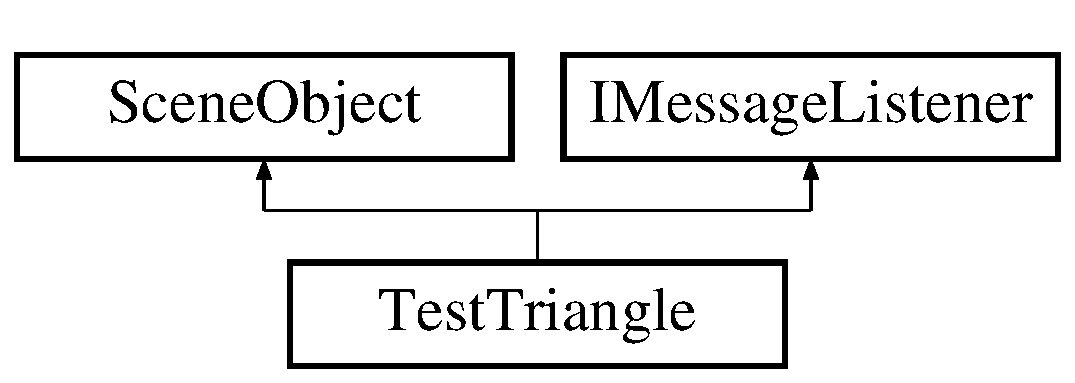
\includegraphics[height=2.000000cm]{class_test_triangle}
\end{center}
\end{figure}
\subsection*{Public Member Functions}
\begin{DoxyCompactItemize}
\item 
\hyperlink{class_test_triangle_ab15daddb4dae8e8ae52aea99afb7d440}{Test\+Triangle} (\hyperlink{class_context}{Context} $\ast$context, std\+::weak\+\_\+ptr$<$ \hyperlink{class_meta_manager}{Meta\+Manager} $>$ managers)
\begin{DoxyCompactList}\small\item\em Default constructor. \end{DoxyCompactList}\item 
\hyperlink{class_test_triangle_aa58d78d1dfb839f32b62881341865ddb}{$\sim$\+Test\+Triangle} ()
\begin{DoxyCompactList}\small\item\em Default destructor. \end{DoxyCompactList}\item 
void \hyperlink{class_test_triangle_a99c4fb3e4da6d1dabf3f9cdeef5b1b31}{step} (double dt) override
\begin{DoxyCompactList}\small\item\em Step the simulation state. \end{DoxyCompactList}\item 
void \hyperlink{class_test_triangle_a0b7b66d114a3d97e524f2d8d9f13a9e7}{predraw} (\hyperlink{class_context}{Context} $\ast$context) override
\begin{DoxyCompactList}\small\item\em Called before the renderer draws the scene This allows the scene objects to do updates that require a graphics context before the graphical state is drawn. \end{DoxyCompactList}\item 
void \hyperlink{class_test_triangle_aadf5ec7f41246e3c114e7f44f009f303}{draw} (\hyperlink{class_context}{Context} $\ast$context, std\+::shared\+\_\+ptr$<$ \hyperlink{class_shader_manager}{Shader\+Manager} $>$ shaders) override
\begin{DoxyCompactList}\small\item\em Draw the object in its current state. \end{DoxyCompactList}\item 
void \hyperlink{class_test_triangle_ac5165e9e0ecdc4b232752b49c1ecbec0}{on\+Message} (std\+::shared\+\_\+ptr$<$ \hyperlink{class_message}{Message} $>$ event) override
\begin{DoxyCompactList}\small\item\em Called when a subscribed event is raised. \end{DoxyCompactList}\end{DoxyCompactItemize}
\subsection*{Private Member Functions}
\begin{DoxyCompactItemize}
\item 
void \hyperlink{class_test_triangle_a52baa578ab64e4fe4cf7ccab89eb51a5}{setup\+Outline} (\hyperlink{class_context}{Context} $\ast$context)
\end{DoxyCompactItemize}
\subsection*{Private Attributes}
\begin{DoxyCompactItemize}
\item 
std\+::shared\+\_\+ptr$<$ \hyperlink{class_model}{Model} $>$ \hyperlink{class_test_triangle_ada9fe71091308f6e50a75f87ff56e14d}{m\+\_\+\+Model}
\item 
std\+::shared\+\_\+ptr$<$ \hyperlink{class_model}{Model} $>$ \hyperlink{class_test_triangle_a6613fd705070b8663027cc14cd542e81}{m\+\_\+\+Outline}
\end{DoxyCompactItemize}
\subsection*{Additional Inherited Members}


\subsection{Detailed Description}


Definition at line 7 of file Test\+Triangle.\+h.



\subsection{Constructor \& Destructor Documentation}
\index{Test\+Triangle@{Test\+Triangle}!Test\+Triangle@{Test\+Triangle}}
\index{Test\+Triangle@{Test\+Triangle}!Test\+Triangle@{Test\+Triangle}}
\subsubsection[{\texorpdfstring{Test\+Triangle(\+Context $\ast$context, std\+::weak\+\_\+ptr$<$ Meta\+Manager $>$ managers)}{TestTriangle(Context *context, std::weak_ptr< MetaManager > managers)}}]{\setlength{\rightskip}{0pt plus 5cm}Test\+Triangle\+::\+Test\+Triangle (
\begin{DoxyParamCaption}
\item[{{\bf Context} $\ast$}]{context, }
\item[{std\+::weak\+\_\+ptr$<$ {\bf Meta\+Manager} $>$}]{managers}
\end{DoxyParamCaption}
)}\hypertarget{class_test_triangle_ab15daddb4dae8e8ae52aea99afb7d440}{}\label{class_test_triangle_ab15daddb4dae8e8ae52aea99afb7d440}


Default constructor. 



Definition at line 6 of file Test\+Triangle.\+cpp.



References Scene\+Object\+::add\+Component(), Model\+::\+Vertex\+::color, f, Message\+System\+::get\+Instance(), m\+\_\+\+Model, Model\+::\+Vertex\+::position, setup\+Outline(), and Message\+System\+::subscribe().

\index{Test\+Triangle@{Test\+Triangle}!````~Test\+Triangle@{$\sim$\+Test\+Triangle}}
\index{````~Test\+Triangle@{$\sim$\+Test\+Triangle}!Test\+Triangle@{Test\+Triangle}}
\subsubsection[{\texorpdfstring{$\sim$\+Test\+Triangle()}{~TestTriangle()}}]{\setlength{\rightskip}{0pt plus 5cm}Test\+Triangle\+::$\sim$\+Test\+Triangle (
\begin{DoxyParamCaption}
{}
\end{DoxyParamCaption}
)}\hypertarget{class_test_triangle_aa58d78d1dfb839f32b62881341865ddb}{}\label{class_test_triangle_aa58d78d1dfb839f32b62881341865ddb}


Default destructor. 



Definition at line 68 of file Test\+Triangle.\+cpp.



References Message\+System\+::get\+Instance(), and Message\+System\+::unsubscribe().



\subsection{Member Function Documentation}
\index{Test\+Triangle@{Test\+Triangle}!draw@{draw}}
\index{draw@{draw}!Test\+Triangle@{Test\+Triangle}}
\subsubsection[{\texorpdfstring{draw(\+Context $\ast$context, std\+::shared\+\_\+ptr$<$ Shader\+Manager $>$ shaders) override}{draw(Context *context, std::shared_ptr< ShaderManager > shaders) override}}]{\setlength{\rightskip}{0pt plus 5cm}void Test\+Triangle\+::draw (
\begin{DoxyParamCaption}
\item[{{\bf Context} $\ast$}]{context, }
\item[{std\+::shared\+\_\+ptr$<$ {\bf Shader\+Manager} $>$}]{shaders}
\end{DoxyParamCaption}
)\hspace{0.3cm}{\ttfamily [override]}, {\ttfamily [virtual]}}\hypertarget{class_test_triangle_aadf5ec7f41246e3c114e7f44f009f303}{}\label{class_test_triangle_aadf5ec7f41246e3c114e7f44f009f303}


Draw the object in its current state. 


\begin{DoxyParams}{Parameters}
{\em context} & Graphics context \\
\hline
{\em shaders} & Shader manager containing shader programs for use \\
\hline
\end{DoxyParams}


Implements \hyperlink{class_scene_object_a9dec6a34922a4063b561d3d16d396ee6}{Scene\+Object}.



Definition at line 84 of file Test\+Triangle.\+cpp.



References m\+\_\+\+Model, and m\+\_\+\+Outline.

\index{Test\+Triangle@{Test\+Triangle}!on\+Message@{on\+Message}}
\index{on\+Message@{on\+Message}!Test\+Triangle@{Test\+Triangle}}
\subsubsection[{\texorpdfstring{on\+Message(std\+::shared\+\_\+ptr$<$ Message $>$ event) override}{onMessage(std::shared_ptr< Message > event) override}}]{\setlength{\rightskip}{0pt plus 5cm}void Test\+Triangle\+::on\+Message (
\begin{DoxyParamCaption}
\item[{std\+::shared\+\_\+ptr$<$ {\bf Message} $>$}]{event}
\end{DoxyParamCaption}
)\hspace{0.3cm}{\ttfamily [override]}, {\ttfamily [virtual]}}\hypertarget{class_test_triangle_ac5165e9e0ecdc4b232752b49c1ecbec0}{}\label{class_test_triangle_ac5165e9e0ecdc4b232752b49c1ecbec0}


Called when a subscribed event is raised. 


\begin{DoxyParams}{Parameters}
{\em event} & Smart pointer to the raised event object \\
\hline
\end{DoxyParams}


Implements \hyperlink{class_i_message_listener_aac85f64eeb587944c59e07f5457b1b82}{I\+Message\+Listener}.



Definition at line 91 of file Test\+Triangle.\+cpp.



References Scene\+Object\+::set\+Dying().

\index{Test\+Triangle@{Test\+Triangle}!predraw@{predraw}}
\index{predraw@{predraw}!Test\+Triangle@{Test\+Triangle}}
\subsubsection[{\texorpdfstring{predraw(\+Context $\ast$context) override}{predraw(Context *context) override}}]{\setlength{\rightskip}{0pt plus 5cm}void Test\+Triangle\+::predraw (
\begin{DoxyParamCaption}
\item[{{\bf Context} $\ast$}]{context}
\end{DoxyParamCaption}
)\hspace{0.3cm}{\ttfamily [override]}, {\ttfamily [virtual]}}\hypertarget{class_test_triangle_a0b7b66d114a3d97e524f2d8d9f13a9e7}{}\label{class_test_triangle_a0b7b66d114a3d97e524f2d8d9f13a9e7}


Called before the renderer draws the scene This allows the scene objects to do updates that require a graphics context before the graphical state is drawn. 


\begin{DoxyParams}{Parameters}
{\em context} & Graphics context \\
\hline
\end{DoxyParams}


Reimplemented from \hyperlink{class_scene_object_a2d5b85ae297772e2f5d0ef6fb920ddf2}{Scene\+Object}.



Definition at line 79 of file Test\+Triangle.\+cpp.



References Scene\+Object\+::predraw().

\index{Test\+Triangle@{Test\+Triangle}!setup\+Outline@{setup\+Outline}}
\index{setup\+Outline@{setup\+Outline}!Test\+Triangle@{Test\+Triangle}}
\subsubsection[{\texorpdfstring{setup\+Outline(\+Context $\ast$context)}{setupOutline(Context *context)}}]{\setlength{\rightskip}{0pt plus 5cm}void Test\+Triangle\+::setup\+Outline (
\begin{DoxyParamCaption}
\item[{{\bf Context} $\ast$}]{context}
\end{DoxyParamCaption}
)\hspace{0.3cm}{\ttfamily [private]}}\hypertarget{class_test_triangle_a52baa578ab64e4fe4cf7ccab89eb51a5}{}\label{class_test_triangle_a52baa578ab64e4fe4cf7ccab89eb51a5}


Definition at line 41 of file Test\+Triangle.\+cpp.



References Model\+::\+Vertex\+::color, f, Lines, m\+\_\+\+Outline, and Model\+::\+Vertex\+::position.



Referenced by Test\+Triangle().

\index{Test\+Triangle@{Test\+Triangle}!step@{step}}
\index{step@{step}!Test\+Triangle@{Test\+Triangle}}
\subsubsection[{\texorpdfstring{step(double dt) override}{step(double dt) override}}]{\setlength{\rightskip}{0pt plus 5cm}void Test\+Triangle\+::step (
\begin{DoxyParamCaption}
\item[{double}]{dt}
\end{DoxyParamCaption}
)\hspace{0.3cm}{\ttfamily [override]}, {\ttfamily [virtual]}}\hypertarget{class_test_triangle_a99c4fb3e4da6d1dabf3f9cdeef5b1b31}{}\label{class_test_triangle_a99c4fb3e4da6d1dabf3f9cdeef5b1b31}


Step the simulation state. 


\begin{DoxyParams}{Parameters}
{\em dt} & Delta-\/time since last step call in seconds \\
\hline
\end{DoxyParams}


Reimplemented from \hyperlink{class_scene_object_a5b69482cadd94997cd09bb145b1986d9}{Scene\+Object}.



Definition at line 74 of file Test\+Triangle.\+cpp.



References Scene\+Object\+::step().



\subsection{Member Data Documentation}
\index{Test\+Triangle@{Test\+Triangle}!m\+\_\+\+Model@{m\+\_\+\+Model}}
\index{m\+\_\+\+Model@{m\+\_\+\+Model}!Test\+Triangle@{Test\+Triangle}}
\subsubsection[{\texorpdfstring{m\+\_\+\+Model}{m_Model}}]{\setlength{\rightskip}{0pt plus 5cm}std\+::shared\+\_\+ptr$<${\bf Model}$>$ Test\+Triangle\+::m\+\_\+\+Model\hspace{0.3cm}{\ttfamily [private]}}\hypertarget{class_test_triangle_ada9fe71091308f6e50a75f87ff56e14d}{}\label{class_test_triangle_ada9fe71091308f6e50a75f87ff56e14d}


Definition at line 47 of file Test\+Triangle.\+h.



Referenced by draw(), and Test\+Triangle().

\index{Test\+Triangle@{Test\+Triangle}!m\+\_\+\+Outline@{m\+\_\+\+Outline}}
\index{m\+\_\+\+Outline@{m\+\_\+\+Outline}!Test\+Triangle@{Test\+Triangle}}
\subsubsection[{\texorpdfstring{m\+\_\+\+Outline}{m_Outline}}]{\setlength{\rightskip}{0pt plus 5cm}std\+::shared\+\_\+ptr$<${\bf Model}$>$ Test\+Triangle\+::m\+\_\+\+Outline\hspace{0.3cm}{\ttfamily [private]}}\hypertarget{class_test_triangle_a6613fd705070b8663027cc14cd542e81}{}\label{class_test_triangle_a6613fd705070b8663027cc14cd542e81}


Definition at line 48 of file Test\+Triangle.\+h.



Referenced by draw(), and setup\+Outline().



The documentation for this class was generated from the following files\+:\begin{DoxyCompactItemize}
\item 
Lunar\+Drift/game/scenes/alphaspace/\hyperlink{_test_triangle_8h}{Test\+Triangle.\+h}\item 
Lunar\+Drift/game/scenes/alphaspace/\hyperlink{_test_triangle_8cpp}{Test\+Triangle.\+cpp}\end{DoxyCompactItemize}

\hypertarget{class_texture}{}\section{Texture Class Reference}
\label{class_texture}\index{Texture@{Texture}}


{\ttfamily \#include $<$Texture.\+h$>$}

\subsection*{Public Member Functions}
\begin{DoxyCompactItemize}
\item 
\hyperlink{class_texture_a6c275e3f186675ff6ed73ccf970e552f}{Texture} ()
\item 
\hyperlink{class_texture_a09c4bcb7462f64c1d20fa69dba3cee8a}{$\sim$\+Texture} ()
\end{DoxyCompactItemize}


\subsection{Detailed Description}


Definition at line 5 of file Texture.\+h.



\subsection{Constructor \& Destructor Documentation}
\index{Texture@{Texture}!Texture@{Texture}}
\index{Texture@{Texture}!Texture@{Texture}}
\subsubsection[{\texorpdfstring{Texture()}{Texture()}}]{\setlength{\rightskip}{0pt plus 5cm}Texture\+::\+Texture (
\begin{DoxyParamCaption}
{}
\end{DoxyParamCaption}
)}\hypertarget{class_texture_a6c275e3f186675ff6ed73ccf970e552f}{}\label{class_texture_a6c275e3f186675ff6ed73ccf970e552f}
Default constructor 

Definition at line 3 of file Texture.\+cpp.

\index{Texture@{Texture}!````~Texture@{$\sim$\+Texture}}
\index{````~Texture@{$\sim$\+Texture}!Texture@{Texture}}
\subsubsection[{\texorpdfstring{$\sim$\+Texture()}{~Texture()}}]{\setlength{\rightskip}{0pt plus 5cm}Texture\+::$\sim$\+Texture (
\begin{DoxyParamCaption}
{}
\end{DoxyParamCaption}
)}\hypertarget{class_texture_a09c4bcb7462f64c1d20fa69dba3cee8a}{}\label{class_texture_a09c4bcb7462f64c1d20fa69dba3cee8a}
Default destructor 

Definition at line 8 of file Texture.\+cpp.



The documentation for this class was generated from the following files\+:\begin{DoxyCompactItemize}
\item 
Lunar\+Drift/engine/graphics/\hyperlink{_texture_8h}{Texture.\+h}\item 
Lunar\+Drift/engine/graphics/\hyperlink{_texture_8cpp}{Texture.\+cpp}\end{DoxyCompactItemize}

\hypertarget{class_texture_manager}{}\section{Texture\+Manager Class Reference}
\label{class_texture_manager}\index{Texture\+Manager@{Texture\+Manager}}


{\ttfamily \#include $<$Texture\+Manager.\+h$>$}

Inheritance diagram for Texture\+Manager\+:\begin{figure}[H]
\begin{center}
\leavevmode
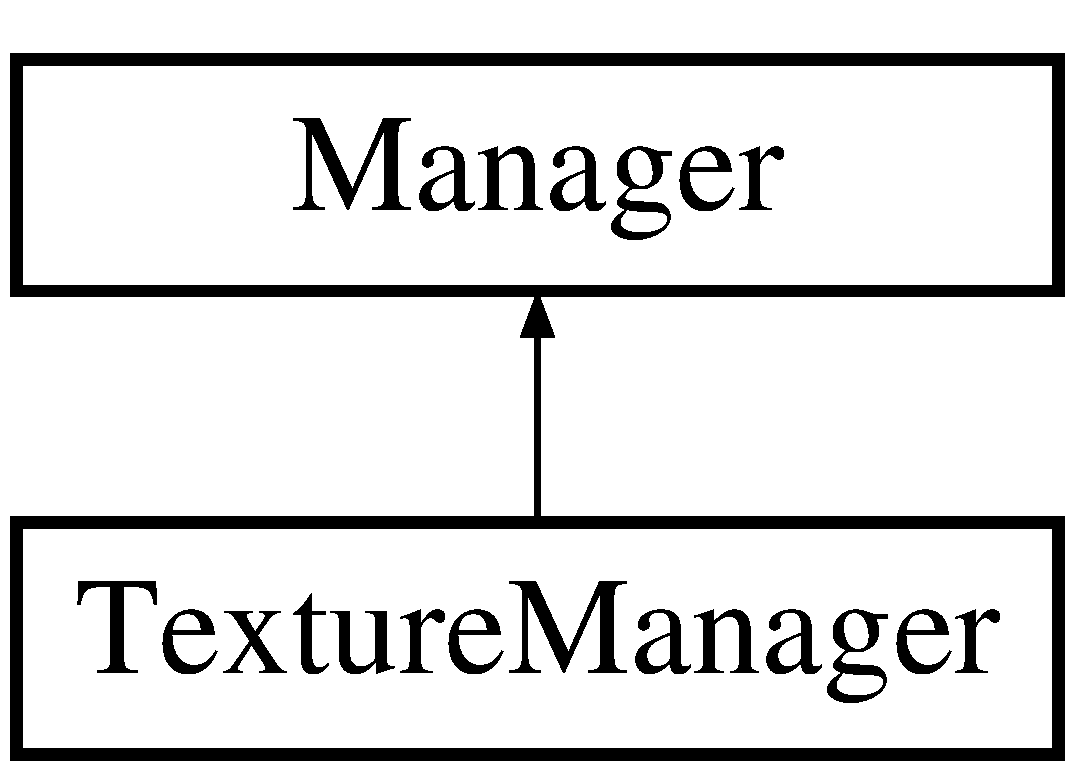
\includegraphics[height=2.000000cm]{class_texture_manager}
\end{center}
\end{figure}
\subsection*{Public Member Functions}
\begin{DoxyCompactItemize}
\item 
\hyperlink{class_texture_manager_ad76abb178b37cedf4514eb0154349935}{Texture\+Manager} ()
\item 
\hyperlink{class_texture_manager_a001d6d74674961db79987e3222682576}{$\sim$\+Texture\+Manager} ()
\item 
std\+::weak\+\_\+ptr$<$ \hyperlink{class_texture}{Texture} $>$ \hyperlink{class_texture_manager_ace3da9513d2c0cb1bdcec6652a6318f9}{get\+Tex} (\hyperlink{class_context}{Context} $\ast$context, const std\+::string \&path)
\item 
std\+::weak\+\_\+ptr$<$ \hyperlink{class_texture}{Texture} $>$ \hyperlink{class_texture_manager_aba074bba0c567f28c94d0c88678fff97}{get\+Tex} (const std\+::string \&path)
\end{DoxyCompactItemize}
\subsection*{Private Attributes}
\begin{DoxyCompactItemize}
\item 
std\+::map$<$ std\+::string, std\+::shared\+\_\+ptr$<$ \hyperlink{class_texture}{Texture} $>$ $>$ \hyperlink{class_texture_manager_a7cf0073a30a272f5dd4660026de58b08}{m\+\_\+\+Textures}
\end{DoxyCompactItemize}


\subsection{Detailed Description}


Definition at line 7 of file Texture\+Manager.\+h.



\subsection{Constructor \& Destructor Documentation}
\index{Texture\+Manager@{Texture\+Manager}!Texture\+Manager@{Texture\+Manager}}
\index{Texture\+Manager@{Texture\+Manager}!Texture\+Manager@{Texture\+Manager}}
\subsubsection[{\texorpdfstring{Texture\+Manager()}{TextureManager()}}]{\setlength{\rightskip}{0pt plus 5cm}Texture\+Manager\+::\+Texture\+Manager (
\begin{DoxyParamCaption}
{}
\end{DoxyParamCaption}
)}\hypertarget{class_texture_manager_ad76abb178b37cedf4514eb0154349935}{}\label{class_texture_manager_ad76abb178b37cedf4514eb0154349935}


Definition at line 4 of file Texture\+Manager.\+cpp.

\index{Texture\+Manager@{Texture\+Manager}!````~Texture\+Manager@{$\sim$\+Texture\+Manager}}
\index{````~Texture\+Manager@{$\sim$\+Texture\+Manager}!Texture\+Manager@{Texture\+Manager}}
\subsubsection[{\texorpdfstring{$\sim$\+Texture\+Manager()}{~TextureManager()}}]{\setlength{\rightskip}{0pt plus 5cm}Texture\+Manager\+::$\sim$\+Texture\+Manager (
\begin{DoxyParamCaption}
{}
\end{DoxyParamCaption}
)}\hypertarget{class_texture_manager_a001d6d74674961db79987e3222682576}{}\label{class_texture_manager_a001d6d74674961db79987e3222682576}


Definition at line 8 of file Texture\+Manager.\+cpp.



\subsection{Member Function Documentation}
\index{Texture\+Manager@{Texture\+Manager}!get\+Tex@{get\+Tex}}
\index{get\+Tex@{get\+Tex}!Texture\+Manager@{Texture\+Manager}}
\subsubsection[{\texorpdfstring{get\+Tex(\+Context $\ast$context, const std\+::string \&path)}{getTex(Context *context, const std::string &path)}}]{\setlength{\rightskip}{0pt plus 5cm}std\+::weak\+\_\+ptr$<$ {\bf Texture} $>$ Texture\+Manager\+::get\+Tex (
\begin{DoxyParamCaption}
\item[{{\bf Context} $\ast$}]{context, }
\item[{const std\+::string \&}]{path}
\end{DoxyParamCaption}
)}\hypertarget{class_texture_manager_ace3da9513d2c0cb1bdcec6652a6318f9}{}\label{class_texture_manager_ace3da9513d2c0cb1bdcec6652a6318f9}


Definition at line 13 of file Texture\+Manager.\+cpp.



References m\+\_\+\+Textures.

\index{Texture\+Manager@{Texture\+Manager}!get\+Tex@{get\+Tex}}
\index{get\+Tex@{get\+Tex}!Texture\+Manager@{Texture\+Manager}}
\subsubsection[{\texorpdfstring{get\+Tex(const std\+::string \&path)}{getTex(const std::string &path)}}]{\setlength{\rightskip}{0pt plus 5cm}std\+::weak\+\_\+ptr$<$ {\bf Texture} $>$ Texture\+Manager\+::get\+Tex (
\begin{DoxyParamCaption}
\item[{const std\+::string \&}]{path}
\end{DoxyParamCaption}
)}\hypertarget{class_texture_manager_aba074bba0c567f28c94d0c88678fff97}{}\label{class_texture_manager_aba074bba0c567f28c94d0c88678fff97}


Definition at line 32 of file Texture\+Manager.\+cpp.



References m\+\_\+\+Textures.



\subsection{Member Data Documentation}
\index{Texture\+Manager@{Texture\+Manager}!m\+\_\+\+Textures@{m\+\_\+\+Textures}}
\index{m\+\_\+\+Textures@{m\+\_\+\+Textures}!Texture\+Manager@{Texture\+Manager}}
\subsubsection[{\texorpdfstring{m\+\_\+\+Textures}{m_Textures}}]{\setlength{\rightskip}{0pt plus 5cm}std\+::map$<$std\+::string, std\+::shared\+\_\+ptr$<${\bf Texture}$>$ $>$ Texture\+Manager\+::m\+\_\+\+Textures\hspace{0.3cm}{\ttfamily [private]}}\hypertarget{class_texture_manager_a7cf0073a30a272f5dd4660026de58b08}{}\label{class_texture_manager_a7cf0073a30a272f5dd4660026de58b08}


Definition at line 20 of file Texture\+Manager.\+h.



Referenced by get\+Tex().



The documentation for this class was generated from the following files\+:\begin{DoxyCompactItemize}
\item 
Lunar\+Drift/engine/managers/\hyperlink{_texture_manager_8h}{Texture\+Manager.\+h}\item 
Lunar\+Drift/engine/managers/\hyperlink{_texture_manager_8cpp}{Texture\+Manager.\+cpp}\end{DoxyCompactItemize}

\hypertarget{class_unsupported_feature_exception}{}\section{Unsupported\+Feature\+Exception Class Reference}
\label{class_unsupported_feature_exception}\index{Unsupported\+Feature\+Exception@{Unsupported\+Feature\+Exception}}


Exception raised whenever a core feature is unsupported.  




{\ttfamily \#include $<$Unsupported\+Feature\+Exception.\+h$>$}

Inheritance diagram for Unsupported\+Feature\+Exception\+:\begin{figure}[H]
\begin{center}
\leavevmode
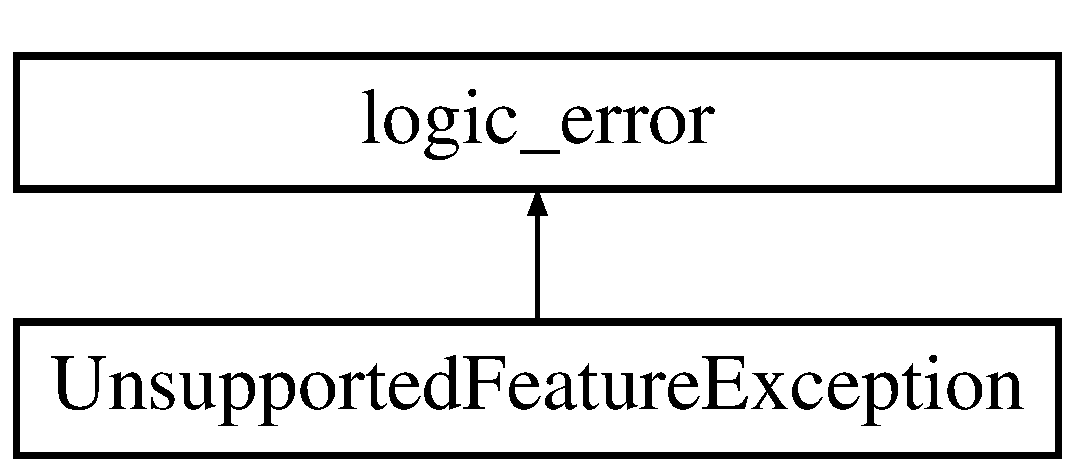
\includegraphics[height=2.000000cm]{class_unsupported_feature_exception}
\end{center}
\end{figure}
\subsection*{Public Member Functions}
\begin{DoxyCompactItemize}
\item 
\hyperlink{class_unsupported_feature_exception_ab9261396c65882bea86a7a4f325e7350}{Unsupported\+Feature\+Exception} (const std\+::string \&feature, const std\+::string \&reason)
\begin{DoxyCompactList}\small\item\em Default constructor. \end{DoxyCompactList}\item 
const std\+::string \& \hyperlink{class_unsupported_feature_exception_aaadf83688501e488262257f527fc520b}{get\+Feature} () const 
\item 
const std\+::string \& \hyperlink{class_unsupported_feature_exception_af22845124ebf0afab42998d5babed4b4}{get\+Reason} () const 
\end{DoxyCompactItemize}
\subsection*{Private Attributes}
\begin{DoxyCompactItemize}
\item 
const std\+::string \& \hyperlink{class_unsupported_feature_exception_a517eaef16c6ed4468d71121cd6ea37d3}{m\+\_\+\+Feature}
\item 
const std\+::string \& \hyperlink{class_unsupported_feature_exception_a0d435f85891b5aea836729f196088ccf}{m\+\_\+\+Reason}
\end{DoxyCompactItemize}


\subsection{Detailed Description}
Exception raised whenever a core feature is unsupported. 

\begin{DoxyAuthor}{Author}
Hayley Hatton 
\end{DoxyAuthor}
\begin{DoxyDate}{Date}
20/02/2016 
\end{DoxyDate}


Definition at line 12 of file Unsupported\+Feature\+Exception.\+h.



\subsection{Constructor \& Destructor Documentation}
\index{Unsupported\+Feature\+Exception@{Unsupported\+Feature\+Exception}!Unsupported\+Feature\+Exception@{Unsupported\+Feature\+Exception}}
\index{Unsupported\+Feature\+Exception@{Unsupported\+Feature\+Exception}!Unsupported\+Feature\+Exception@{Unsupported\+Feature\+Exception}}
\subsubsection[{\texorpdfstring{Unsupported\+Feature\+Exception(const std\+::string \&feature, const std\+::string \&reason)}{UnsupportedFeatureException(const std::string &feature, const std::string &reason)}}]{\setlength{\rightskip}{0pt plus 5cm}Unsupported\+Feature\+Exception\+::\+Unsupported\+Feature\+Exception (
\begin{DoxyParamCaption}
\item[{const std\+::string \&}]{feature, }
\item[{const std\+::string \&}]{reason}
\end{DoxyParamCaption}
)}\hypertarget{class_unsupported_feature_exception_ab9261396c65882bea86a7a4f325e7350}{}\label{class_unsupported_feature_exception_ab9261396c65882bea86a7a4f325e7350}


Default constructor. 


\begin{DoxyParams}{Parameters}
{\em feature} & Engine feature that\textquotesingle{}s not supported. \\
\hline
{\em reason} & The reason behind why they\textquotesingle{}re not supported (optional). \\
\hline
\end{DoxyParams}


Definition at line 3 of file Unsupported\+Feature\+Exception.\+cpp.



\subsection{Member Function Documentation}
\index{Unsupported\+Feature\+Exception@{Unsupported\+Feature\+Exception}!get\+Feature@{get\+Feature}}
\index{get\+Feature@{get\+Feature}!Unsupported\+Feature\+Exception@{Unsupported\+Feature\+Exception}}
\subsubsection[{\texorpdfstring{get\+Feature() const }{getFeature() const }}]{\setlength{\rightskip}{0pt plus 5cm}const std\+::string\& Unsupported\+Feature\+Exception\+::get\+Feature (
\begin{DoxyParamCaption}
{}
\end{DoxyParamCaption}
) const\hspace{0.3cm}{\ttfamily [inline]}}\hypertarget{class_unsupported_feature_exception_aaadf83688501e488262257f527fc520b}{}\label{class_unsupported_feature_exception_aaadf83688501e488262257f527fc520b}


Definition at line 25 of file Unsupported\+Feature\+Exception.\+h.



References m\+\_\+\+Feature.



Referenced by Window\+P\+C\+::rendering\+Thread(), and Win\+Main().

\index{Unsupported\+Feature\+Exception@{Unsupported\+Feature\+Exception}!get\+Reason@{get\+Reason}}
\index{get\+Reason@{get\+Reason}!Unsupported\+Feature\+Exception@{Unsupported\+Feature\+Exception}}
\subsubsection[{\texorpdfstring{get\+Reason() const }{getReason() const }}]{\setlength{\rightskip}{0pt plus 5cm}const std\+::string\& Unsupported\+Feature\+Exception\+::get\+Reason (
\begin{DoxyParamCaption}
{}
\end{DoxyParamCaption}
) const\hspace{0.3cm}{\ttfamily [inline]}}\hypertarget{class_unsupported_feature_exception_af22845124ebf0afab42998d5babed4b4}{}\label{class_unsupported_feature_exception_af22845124ebf0afab42998d5babed4b4}


Definition at line 27 of file Unsupported\+Feature\+Exception.\+h.



References m\+\_\+\+Reason.



Referenced by Window\+P\+C\+::rendering\+Thread(), and Win\+Main().



\subsection{Member Data Documentation}
\index{Unsupported\+Feature\+Exception@{Unsupported\+Feature\+Exception}!m\+\_\+\+Feature@{m\+\_\+\+Feature}}
\index{m\+\_\+\+Feature@{m\+\_\+\+Feature}!Unsupported\+Feature\+Exception@{Unsupported\+Feature\+Exception}}
\subsubsection[{\texorpdfstring{m\+\_\+\+Feature}{m_Feature}}]{\setlength{\rightskip}{0pt plus 5cm}const std\+::string\& Unsupported\+Feature\+Exception\+::m\+\_\+\+Feature\hspace{0.3cm}{\ttfamily [private]}}\hypertarget{class_unsupported_feature_exception_a517eaef16c6ed4468d71121cd6ea37d3}{}\label{class_unsupported_feature_exception_a517eaef16c6ed4468d71121cd6ea37d3}


Definition at line 30 of file Unsupported\+Feature\+Exception.\+h.



Referenced by get\+Feature().

\index{Unsupported\+Feature\+Exception@{Unsupported\+Feature\+Exception}!m\+\_\+\+Reason@{m\+\_\+\+Reason}}
\index{m\+\_\+\+Reason@{m\+\_\+\+Reason}!Unsupported\+Feature\+Exception@{Unsupported\+Feature\+Exception}}
\subsubsection[{\texorpdfstring{m\+\_\+\+Reason}{m_Reason}}]{\setlength{\rightskip}{0pt plus 5cm}const std\+::string\& Unsupported\+Feature\+Exception\+::m\+\_\+\+Reason\hspace{0.3cm}{\ttfamily [private]}}\hypertarget{class_unsupported_feature_exception_a0d435f85891b5aea836729f196088ccf}{}\label{class_unsupported_feature_exception_a0d435f85891b5aea836729f196088ccf}


Definition at line 31 of file Unsupported\+Feature\+Exception.\+h.



Referenced by get\+Reason().



The documentation for this class was generated from the following files\+:\begin{DoxyCompactItemize}
\item 
Lunar\+Drift/engine/exceptions/\hyperlink{_unsupported_feature_exception_8h}{Unsupported\+Feature\+Exception.\+h}\item 
Lunar\+Drift/engine/exceptions/\hyperlink{_unsupported_feature_exception_8cpp}{Unsupported\+Feature\+Exception.\+cpp}\end{DoxyCompactItemize}

\hypertarget{struct_model_loader_1_1_vertex}{}\section{Model\+Loader\+:\+:Vertex Struct Reference}
\label{struct_model_loader_1_1_vertex}\index{Model\+Loader\+::\+Vertex@{Model\+Loader\+::\+Vertex}}
\subsection*{Public Attributes}
\begin{DoxyCompactItemize}
\item 
glm\+::vec3 \hyperlink{struct_model_loader_1_1_vertex_a78385e6b324c9f786e7f4e14263ca026}{position}
\item 
glm\+::vec3 \hyperlink{struct_model_loader_1_1_vertex_a0d1ac4c30a3a1e4645ea14332d86b035}{normal}
\item 
glm\+::vec3 \hyperlink{struct_model_loader_1_1_vertex_a4cecec2539987da6dfb1a325baf9ae16}{color}
\item 
glm\+::vec2 \hyperlink{struct_model_loader_1_1_vertex_a8821e887b456902f93bf0e16f58a72db}{tex\+Coord}
\end{DoxyCompactItemize}


\subsection{Detailed Description}


Definition at line 65 of file Model\+Loader.\+h.



\subsection{Member Data Documentation}
\index{Model\+Loader\+::\+Vertex@{Model\+Loader\+::\+Vertex}!color@{color}}
\index{color@{color}!Model\+Loader\+::\+Vertex@{Model\+Loader\+::\+Vertex}}
\subsubsection[{\texorpdfstring{color}{color}}]{\setlength{\rightskip}{0pt plus 5cm}glm\+::vec3 Model\+Loader\+::\+Vertex\+::color}\hypertarget{struct_model_loader_1_1_vertex_a4cecec2539987da6dfb1a325baf9ae16}{}\label{struct_model_loader_1_1_vertex_a4cecec2539987da6dfb1a325baf9ae16}


Definition at line 69 of file Model\+Loader.\+h.



Referenced by Model\+Loader\+::compile(), and Model\+Loader\+::load().

\index{Model\+Loader\+::\+Vertex@{Model\+Loader\+::\+Vertex}!normal@{normal}}
\index{normal@{normal}!Model\+Loader\+::\+Vertex@{Model\+Loader\+::\+Vertex}}
\subsubsection[{\texorpdfstring{normal}{normal}}]{\setlength{\rightskip}{0pt plus 5cm}glm\+::vec3 Model\+Loader\+::\+Vertex\+::normal}\hypertarget{struct_model_loader_1_1_vertex_a0d1ac4c30a3a1e4645ea14332d86b035}{}\label{struct_model_loader_1_1_vertex_a0d1ac4c30a3a1e4645ea14332d86b035}


Definition at line 68 of file Model\+Loader.\+h.



Referenced by Model\+Loader\+::compile(), and Model\+Loader\+::load().

\index{Model\+Loader\+::\+Vertex@{Model\+Loader\+::\+Vertex}!position@{position}}
\index{position@{position}!Model\+Loader\+::\+Vertex@{Model\+Loader\+::\+Vertex}}
\subsubsection[{\texorpdfstring{position}{position}}]{\setlength{\rightskip}{0pt plus 5cm}glm\+::vec3 Model\+Loader\+::\+Vertex\+::position}\hypertarget{struct_model_loader_1_1_vertex_a78385e6b324c9f786e7f4e14263ca026}{}\label{struct_model_loader_1_1_vertex_a78385e6b324c9f786e7f4e14263ca026}


Definition at line 67 of file Model\+Loader.\+h.



Referenced by Model\+Loader\+::compile(), and Model\+Loader\+::load().

\index{Model\+Loader\+::\+Vertex@{Model\+Loader\+::\+Vertex}!tex\+Coord@{tex\+Coord}}
\index{tex\+Coord@{tex\+Coord}!Model\+Loader\+::\+Vertex@{Model\+Loader\+::\+Vertex}}
\subsubsection[{\texorpdfstring{tex\+Coord}{texCoord}}]{\setlength{\rightskip}{0pt plus 5cm}glm\+::vec2 Model\+Loader\+::\+Vertex\+::tex\+Coord}\hypertarget{struct_model_loader_1_1_vertex_a8821e887b456902f93bf0e16f58a72db}{}\label{struct_model_loader_1_1_vertex_a8821e887b456902f93bf0e16f58a72db}


Definition at line 70 of file Model\+Loader.\+h.



Referenced by Model\+Loader\+::compile(), and Model\+Loader\+::load().



The documentation for this struct was generated from the following file\+:\begin{DoxyCompactItemize}
\item 
Lunar\+Drift/engine/containers/\hyperlink{_model_loader_8h}{Model\+Loader.\+h}\end{DoxyCompactItemize}

\hypertarget{struct_model_1_1_vertex}{}\section{Model\+:\+:Vertex Struct Reference}
\label{struct_model_1_1_vertex}\index{Model\+::\+Vertex@{Model\+::\+Vertex}}


Predefined vertex format for standard 3D models.  




{\ttfamily \#include $<$Model.\+h$>$}

\subsection*{Public Attributes}
\begin{DoxyCompactItemize}
\item 
glm\+::vec3 \hyperlink{struct_model_1_1_vertex_a27d09cad05dd2a74b8aa44f934441a9e}{position}
\item 
glm\+::vec3 \hyperlink{struct_model_1_1_vertex_a75c5e19722462c1ef8a5ba863db069ea}{normal}
\item 
glm\+::vec4 \hyperlink{struct_model_1_1_vertex_a5523bdc6906902bc1d88fb01cae1b550}{color}
\item 
glm\+::vec2 \hyperlink{struct_model_1_1_vertex_a45595f4db5a1dc76d9a47434b1eea559}{tex\+Coord}
\end{DoxyCompactItemize}


\subsection{Detailed Description}
Predefined vertex format for standard 3D models. 

Definition at line 38 of file Model.\+h.



\subsection{Member Data Documentation}
\index{Model\+::\+Vertex@{Model\+::\+Vertex}!color@{color}}
\index{color@{color}!Model\+::\+Vertex@{Model\+::\+Vertex}}
\subsubsection[{\texorpdfstring{color}{color}}]{\setlength{\rightskip}{0pt plus 5cm}glm\+::vec4 Model\+::\+Vertex\+::color}\hypertarget{struct_model_1_1_vertex_a5523bdc6906902bc1d88fb01cae1b550}{}\label{struct_model_1_1_vertex_a5523bdc6906902bc1d88fb01cae1b550}


Definition at line 42 of file Model.\+h.



Referenced by Test\+Triangle\+::setup\+Outline(), and Test\+Triangle\+::\+Test\+Triangle().

\index{Model\+::\+Vertex@{Model\+::\+Vertex}!normal@{normal}}
\index{normal@{normal}!Model\+::\+Vertex@{Model\+::\+Vertex}}
\subsubsection[{\texorpdfstring{normal}{normal}}]{\setlength{\rightskip}{0pt plus 5cm}glm\+::vec3 Model\+::\+Vertex\+::normal}\hypertarget{struct_model_1_1_vertex_a75c5e19722462c1ef8a5ba863db069ea}{}\label{struct_model_1_1_vertex_a75c5e19722462c1ef8a5ba863db069ea}


Definition at line 41 of file Model.\+h.

\index{Model\+::\+Vertex@{Model\+::\+Vertex}!position@{position}}
\index{position@{position}!Model\+::\+Vertex@{Model\+::\+Vertex}}
\subsubsection[{\texorpdfstring{position}{position}}]{\setlength{\rightskip}{0pt plus 5cm}glm\+::vec3 Model\+::\+Vertex\+::position}\hypertarget{struct_model_1_1_vertex_a27d09cad05dd2a74b8aa44f934441a9e}{}\label{struct_model_1_1_vertex_a27d09cad05dd2a74b8aa44f934441a9e}


Definition at line 40 of file Model.\+h.



Referenced by Test\+Triangle\+::setup\+Outline(), and Test\+Triangle\+::\+Test\+Triangle().

\index{Model\+::\+Vertex@{Model\+::\+Vertex}!tex\+Coord@{tex\+Coord}}
\index{tex\+Coord@{tex\+Coord}!Model\+::\+Vertex@{Model\+::\+Vertex}}
\subsubsection[{\texorpdfstring{tex\+Coord}{texCoord}}]{\setlength{\rightskip}{0pt plus 5cm}glm\+::vec2 Model\+::\+Vertex\+::tex\+Coord}\hypertarget{struct_model_1_1_vertex_a45595f4db5a1dc76d9a47434b1eea559}{}\label{struct_model_1_1_vertex_a45595f4db5a1dc76d9a47434b1eea559}


Definition at line 43 of file Model.\+h.



The documentation for this struct was generated from the following file\+:\begin{DoxyCompactItemize}
\item 
Lunar\+Drift/engine/containers/\hyperlink{_model_8h}{Model.\+h}\end{DoxyCompactItemize}

\hypertarget{class_vertex_array_object}{}\section{Vertex\+Array\+Object Class Reference}
\label{class_vertex_array_object}\index{Vertex\+Array\+Object@{Vertex\+Array\+Object}}


A buffer object that aggregates V\+B\+Os, Vertex Attributes and I\+B\+Os.  




{\ttfamily \#include $<$Vertex\+Array\+Object.\+h$>$}

\subsection*{Public Member Functions}
\begin{DoxyCompactItemize}
\item 
\hyperlink{class_vertex_array_object_a6fab9649bd299f89f64b8bcc9d6173dd}{Vertex\+Array\+Object} (\hyperlink{class_context}{Context} $\ast$context, std\+::shared\+\_\+ptr$<$ \hyperlink{class_vertex_buffer_object_base}{Vertex\+Buffer\+Object\+Base} $>$ vbo, const std\+::vector$<$ \hyperlink{class_vertex_attribute}{Vertex\+Attribute} $>$ \&attributes, std\+::shared\+\_\+ptr$<$ \hyperlink{class_index_buffer_object}{Index\+Buffer\+Object} $>$ ibo=nullptr)
\begin{DoxyCompactList}\small\item\em Constructs a V\+AO and associates it with the V\+BO and/or I\+BO. \end{DoxyCompactList}\item 
virtual \hyperlink{class_vertex_array_object_a37ca7e8bff292e3f334544dd6ba4ab37}{$\sim$\+Vertex\+Array\+Object} ()
\begin{DoxyCompactList}\small\item\em Default destructor. \end{DoxyCompactList}\item 
void \hyperlink{class_vertex_array_object_aa830fc54932a907bec1858847668734f}{set\+Vertex\+Buffer} (std\+::shared\+\_\+ptr$<$ \hyperlink{class_vertex_buffer_object_base}{Vertex\+Buffer\+Object\+Base} $>$ vbo)
\begin{DoxyCompactList}\small\item\em Associate a \hyperlink{class_vertex_buffer_object}{Vertex\+Buffer\+Object} with the V\+AO. \end{DoxyCompactList}\item 
std\+::shared\+\_\+ptr$<$ \hyperlink{class_vertex_buffer_object_base}{Vertex\+Buffer\+Object\+Base} $>$ \hyperlink{class_vertex_array_object_adf92ade27ac0b57911d1dc1b707fc454}{get\+Vertex\+Buffer} ()
\begin{DoxyCompactList}\small\item\em Access the \hyperlink{class_vertex_buffer_object}{Vertex\+Buffer\+Object} associated with the V\+AO. \end{DoxyCompactList}\item 
void \hyperlink{class_vertex_array_object_aafc38c6ce0a65051996a3eaadb2febcc}{set\+Attribute\+Map} (const std\+::vector$<$ \hyperlink{class_vertex_attribute}{Vertex\+Attribute} $>$ \&attributes)
\begin{DoxyCompactList}\small\item\em Set a new map of attributes to describe the associated vertex data. \end{DoxyCompactList}\item 
const std\+::vector$<$ \hyperlink{class_vertex_attribute}{Vertex\+Attribute} $>$ \& \hyperlink{class_vertex_array_object_a91c81009eb2ab054c57a7053b974421b}{get\+Attribute\+Map} () const 
\begin{DoxyCompactList}\small\item\em Access the map of attributes that describe the vertex data. \end{DoxyCompactList}\item 
void \hyperlink{class_vertex_array_object_a074da4a3d5d45cc4935458b1e5441d61}{set\+Index\+Buffer} (std\+::shared\+\_\+ptr$<$ \hyperlink{class_index_buffer_object}{Index\+Buffer\+Object} $>$ ibo)
\begin{DoxyCompactList}\small\item\em Associate or disassociate an \hyperlink{class_index_buffer_object}{Index\+Buffer\+Object} with the V\+AO. \end{DoxyCompactList}\item 
std\+::shared\+\_\+ptr$<$ \hyperlink{class_index_buffer_object}{Index\+Buffer\+Object} $>$ \hyperlink{class_vertex_array_object_ab1b5d2c13e89a77ff2da97dc3a072ec4}{get\+Index\+Buffer} ()
\begin{DoxyCompactList}\small\item\em Access the \hyperlink{class_index_buffer_object}{Index\+Buffer\+Object} associated with the V\+AO. \end{DoxyCompactList}\item 
void \hyperlink{class_vertex_array_object_a9228fcd314372296db91b65c792f412c}{bind} (\hyperlink{class_context}{Context} $\ast$context, std\+::shared\+\_\+ptr$<$ \hyperlink{class_shader_program}{Shader\+Program} $>$ shader)
\begin{DoxyCompactList}\small\item\em Bind the V\+AO to the Open\+GL state pipeline. \end{DoxyCompactList}\end{DoxyCompactItemize}
\subsection*{Private Attributes}
\begin{DoxyCompactItemize}
\item 
std\+::vector$<$ \hyperlink{class_vertex_attribute}{Vertex\+Attribute} $>$ \hyperlink{class_vertex_array_object_aacb321d71b55ce0f75dfe5b28e8c748c}{m\+\_\+\+Attributes}
\begin{DoxyCompactList}\small\item\em Attribute map for shaders. \end{DoxyCompactList}\item 
std\+::shared\+\_\+ptr$<$ \hyperlink{class_vertex_buffer_object_base}{Vertex\+Buffer\+Object\+Base} $>$ \hyperlink{class_vertex_array_object_a2e6040e6adfc2bbcf29d48013c48af04}{m\+\_\+\+Vertex\+Buffer}
\begin{DoxyCompactList}\small\item\em V\+BO ptr. \end{DoxyCompactList}\item 
std\+::shared\+\_\+ptr$<$ \hyperlink{class_index_buffer_object}{Index\+Buffer\+Object} $>$ \hyperlink{class_vertex_array_object_acd24cb60a9b2efe8e81cf50f1a6ebe1a}{m\+\_\+\+Index\+Buffer}
\begin{DoxyCompactList}\small\item\em I\+BO ptr. \end{DoxyCompactList}\item 
G\+Luint \hyperlink{class_vertex_array_object_a9def0a990bac4db152e962d4d1a84f0f}{m\+\_\+\+V\+AO}
\begin{DoxyCompactList}\small\item\em Open\+G\+L-\/provided V\+AO handle. \end{DoxyCompactList}\end{DoxyCompactItemize}


\subsection{Detailed Description}
A buffer object that aggregates V\+B\+Os, Vertex Attributes and I\+B\+Os. 

\begin{DoxyPrecond}{Precondition}
A valid Open\+GL context must be present to the program 
\end{DoxyPrecond}
\begin{DoxyAuthor}{Author}
Hayley Hatton 
\end{DoxyAuthor}
\begin{DoxyDate}{Date}
20/02/2016 
\end{DoxyDate}
\begin{DoxySeeAlso}{See also}
\hyperlink{class_index_buffer_object}{Index\+Buffer\+Object} 

\hyperlink{class_vertex_buffer_object}{Vertex\+Buffer\+Object} 

\hyperlink{class_vertex_attribute}{Vertex\+Attribute} 
\end{DoxySeeAlso}


Definition at line 17 of file Vertex\+Array\+Object.\+h.



\subsection{Constructor \& Destructor Documentation}
\index{Vertex\+Array\+Object@{Vertex\+Array\+Object}!Vertex\+Array\+Object@{Vertex\+Array\+Object}}
\index{Vertex\+Array\+Object@{Vertex\+Array\+Object}!Vertex\+Array\+Object@{Vertex\+Array\+Object}}
\subsubsection[{\texorpdfstring{Vertex\+Array\+Object(\+Context $\ast$context, std\+::shared\+\_\+ptr$<$ Vertex\+Buffer\+Object\+Base $>$ vbo, const std\+::vector$<$ Vertex\+Attribute $>$ \&attributes, std\+::shared\+\_\+ptr$<$ Index\+Buffer\+Object $>$ ibo=nullptr)}{VertexArrayObject(Context *context, std::shared_ptr< VertexBufferObjectBase > vbo, const std::vector< VertexAttribute > &attributes, std::shared_ptr< IndexBufferObject > ibo=nullptr)}}]{\setlength{\rightskip}{0pt plus 5cm}Vertex\+Array\+Object\+::\+Vertex\+Array\+Object (
\begin{DoxyParamCaption}
\item[{{\bf Context} $\ast$}]{context, }
\item[{std\+::shared\+\_\+ptr$<$ {\bf Vertex\+Buffer\+Object\+Base} $>$}]{vbo, }
\item[{const std\+::vector$<$ {\bf Vertex\+Attribute} $>$ \&}]{attributes, }
\item[{std\+::shared\+\_\+ptr$<$ {\bf Index\+Buffer\+Object} $>$}]{ibo = {\ttfamily nullptr}}
\end{DoxyParamCaption}
)}\hypertarget{class_vertex_array_object_a6fab9649bd299f89f64b8bcc9d6173dd}{}\label{class_vertex_array_object_a6fab9649bd299f89f64b8bcc9d6173dd}


Constructs a V\+AO and associates it with the V\+BO and/or I\+BO. 


\begin{DoxyParams}{Parameters}
{\em context} & Graphics context \\
\hline
{\em vbo} & Vertex buffer object ptr to associate with V\+AO \\
\hline
{\em attributes} & Attribute map for describing vertex input to shaders \\
\hline
{\em ibo} & Index buffer object ptr to associate with V\+AO \\
\hline
\end{DoxyParams}


Definition at line 5 of file Vertex\+Array\+Object.\+cpp.



References m\+\_\+\+V\+AO.

\index{Vertex\+Array\+Object@{Vertex\+Array\+Object}!````~Vertex\+Array\+Object@{$\sim$\+Vertex\+Array\+Object}}
\index{````~Vertex\+Array\+Object@{$\sim$\+Vertex\+Array\+Object}!Vertex\+Array\+Object@{Vertex\+Array\+Object}}
\subsubsection[{\texorpdfstring{$\sim$\+Vertex\+Array\+Object()}{~VertexArrayObject()}}]{\setlength{\rightskip}{0pt plus 5cm}Vertex\+Array\+Object\+::$\sim$\+Vertex\+Array\+Object (
\begin{DoxyParamCaption}
{}
\end{DoxyParamCaption}
)\hspace{0.3cm}{\ttfamily [virtual]}}\hypertarget{class_vertex_array_object_a37ca7e8bff292e3f334544dd6ba4ab37}{}\label{class_vertex_array_object_a37ca7e8bff292e3f334544dd6ba4ab37}


Default destructor. 



Definition at line 30 of file Vertex\+Array\+Object.\+cpp.



References m\+\_\+\+V\+AO.



\subsection{Member Function Documentation}
\index{Vertex\+Array\+Object@{Vertex\+Array\+Object}!bind@{bind}}
\index{bind@{bind}!Vertex\+Array\+Object@{Vertex\+Array\+Object}}
\subsubsection[{\texorpdfstring{bind(\+Context $\ast$context, std\+::shared\+\_\+ptr$<$ Shader\+Program $>$ shader)}{bind(Context *context, std::shared_ptr< ShaderProgram > shader)}}]{\setlength{\rightskip}{0pt plus 5cm}void Vertex\+Array\+Object\+::bind (
\begin{DoxyParamCaption}
\item[{{\bf Context} $\ast$}]{context, }
\item[{std\+::shared\+\_\+ptr$<$ {\bf Shader\+Program} $>$}]{shader}
\end{DoxyParamCaption}
)}\hypertarget{class_vertex_array_object_a9228fcd314372296db91b65c792f412c}{}\label{class_vertex_array_object_a9228fcd314372296db91b65c792f412c}


Bind the V\+AO to the Open\+GL state pipeline. 


\begin{DoxyParams}{Parameters}
{\em context} & Graphics context \\
\hline
{\em shader} & Shader program to use with the V\+AO \\
\hline
\end{DoxyParams}


Definition at line 54 of file Vertex\+Array\+Object.\+cpp.



References m\+\_\+\+Attributes, m\+\_\+\+Index\+Buffer, m\+\_\+\+V\+AO, and m\+\_\+\+Vertex\+Buffer.



Referenced by get\+Index\+Buffer().

\index{Vertex\+Array\+Object@{Vertex\+Array\+Object}!get\+Attribute\+Map@{get\+Attribute\+Map}}
\index{get\+Attribute\+Map@{get\+Attribute\+Map}!Vertex\+Array\+Object@{Vertex\+Array\+Object}}
\subsubsection[{\texorpdfstring{get\+Attribute\+Map() const }{getAttributeMap() const }}]{\setlength{\rightskip}{0pt plus 5cm}const std\+::vector$<${\bf Vertex\+Attribute}$>$\& Vertex\+Array\+Object\+::get\+Attribute\+Map (
\begin{DoxyParamCaption}
{}
\end{DoxyParamCaption}
) const\hspace{0.3cm}{\ttfamily [inline]}}\hypertarget{class_vertex_array_object_a91c81009eb2ab054c57a7053b974421b}{}\label{class_vertex_array_object_a91c81009eb2ab054c57a7053b974421b}


Access the map of attributes that describe the vertex data. 

\begin{DoxyReturn}{Returns}
Vector of attribute descriptors 
\end{DoxyReturn}


Definition at line 61 of file Vertex\+Array\+Object.\+h.



References m\+\_\+\+Attributes, and set\+Index\+Buffer().

\index{Vertex\+Array\+Object@{Vertex\+Array\+Object}!get\+Index\+Buffer@{get\+Index\+Buffer}}
\index{get\+Index\+Buffer@{get\+Index\+Buffer}!Vertex\+Array\+Object@{Vertex\+Array\+Object}}
\subsubsection[{\texorpdfstring{get\+Index\+Buffer()}{getIndexBuffer()}}]{\setlength{\rightskip}{0pt plus 5cm}std\+::shared\+\_\+ptr$<${\bf Index\+Buffer\+Object}$>$ Vertex\+Array\+Object\+::get\+Index\+Buffer (
\begin{DoxyParamCaption}
{}
\end{DoxyParamCaption}
)\hspace{0.3cm}{\ttfamily [inline]}}\hypertarget{class_vertex_array_object_ab1b5d2c13e89a77ff2da97dc3a072ec4}{}\label{class_vertex_array_object_ab1b5d2c13e89a77ff2da97dc3a072ec4}


Access the \hyperlink{class_index_buffer_object}{Index\+Buffer\+Object} associated with the V\+AO. 

\begin{DoxyReturn}{Returns}
Smart ptr (or nullptr) to the underlying \hyperlink{class_index_buffer_object}{Index\+Buffer\+Object} 
\end{DoxyReturn}


Definition at line 75 of file Vertex\+Array\+Object.\+h.



References bind(), and m\+\_\+\+Index\+Buffer.

\index{Vertex\+Array\+Object@{Vertex\+Array\+Object}!get\+Vertex\+Buffer@{get\+Vertex\+Buffer}}
\index{get\+Vertex\+Buffer@{get\+Vertex\+Buffer}!Vertex\+Array\+Object@{Vertex\+Array\+Object}}
\subsubsection[{\texorpdfstring{get\+Vertex\+Buffer()}{getVertexBuffer()}}]{\setlength{\rightskip}{0pt plus 5cm}std\+::shared\+\_\+ptr$<${\bf Vertex\+Buffer\+Object\+Base}$>$ Vertex\+Array\+Object\+::get\+Vertex\+Buffer (
\begin{DoxyParamCaption}
{}
\end{DoxyParamCaption}
)\hspace{0.3cm}{\ttfamily [inline]}}\hypertarget{class_vertex_array_object_adf92ade27ac0b57911d1dc1b707fc454}{}\label{class_vertex_array_object_adf92ade27ac0b57911d1dc1b707fc454}


Access the \hyperlink{class_vertex_buffer_object}{Vertex\+Buffer\+Object} associated with the V\+AO. 

\begin{DoxyReturn}{Returns}
Smart ptr to the underlying \hyperlink{class_vertex_buffer_object}{Vertex\+Buffer\+Object} 
\end{DoxyReturn}


Definition at line 47 of file Vertex\+Array\+Object.\+h.



References m\+\_\+\+Vertex\+Buffer, and set\+Attribute\+Map().

\index{Vertex\+Array\+Object@{Vertex\+Array\+Object}!set\+Attribute\+Map@{set\+Attribute\+Map}}
\index{set\+Attribute\+Map@{set\+Attribute\+Map}!Vertex\+Array\+Object@{Vertex\+Array\+Object}}
\subsubsection[{\texorpdfstring{set\+Attribute\+Map(const std\+::vector$<$ Vertex\+Attribute $>$ \&attributes)}{setAttributeMap(const std::vector< VertexAttribute > &attributes)}}]{\setlength{\rightskip}{0pt plus 5cm}void Vertex\+Array\+Object\+::set\+Attribute\+Map (
\begin{DoxyParamCaption}
\item[{const std\+::vector$<$ {\bf Vertex\+Attribute} $>$ \&}]{attributes}
\end{DoxyParamCaption}
)}\hypertarget{class_vertex_array_object_aafc38c6ce0a65051996a3eaadb2febcc}{}\label{class_vertex_array_object_aafc38c6ce0a65051996a3eaadb2febcc}


Set a new map of attributes to describe the associated vertex data. 


\begin{DoxyParams}{Parameters}
{\em attributes} & Attribute map for describing vertex input to shaders \\
\hline
\end{DoxyParams}


Definition at line 36 of file Vertex\+Array\+Object.\+cpp.



References m\+\_\+\+Attributes.



Referenced by get\+Vertex\+Buffer().

\index{Vertex\+Array\+Object@{Vertex\+Array\+Object}!set\+Index\+Buffer@{set\+Index\+Buffer}}
\index{set\+Index\+Buffer@{set\+Index\+Buffer}!Vertex\+Array\+Object@{Vertex\+Array\+Object}}
\subsubsection[{\texorpdfstring{set\+Index\+Buffer(std\+::shared\+\_\+ptr$<$ Index\+Buffer\+Object $>$ ibo)}{setIndexBuffer(std::shared_ptr< IndexBufferObject > ibo)}}]{\setlength{\rightskip}{0pt plus 5cm}void Vertex\+Array\+Object\+::set\+Index\+Buffer (
\begin{DoxyParamCaption}
\item[{std\+::shared\+\_\+ptr$<$ {\bf Index\+Buffer\+Object} $>$}]{ibo}
\end{DoxyParamCaption}
)}\hypertarget{class_vertex_array_object_a074da4a3d5d45cc4935458b1e5441d61}{}\label{class_vertex_array_object_a074da4a3d5d45cc4935458b1e5441d61}


Associate or disassociate an \hyperlink{class_index_buffer_object}{Index\+Buffer\+Object} with the V\+AO. 


\begin{DoxyParams}{Parameters}
{\em ibo} & \hyperlink{class_index_buffer_object}{Index\+Buffer\+Object} ptr (or nullptr) to associate with the V\+AO \\
\hline
\end{DoxyParams}


Definition at line 48 of file Vertex\+Array\+Object.\+cpp.



References m\+\_\+\+Index\+Buffer.



Referenced by get\+Attribute\+Map().

\index{Vertex\+Array\+Object@{Vertex\+Array\+Object}!set\+Vertex\+Buffer@{set\+Vertex\+Buffer}}
\index{set\+Vertex\+Buffer@{set\+Vertex\+Buffer}!Vertex\+Array\+Object@{Vertex\+Array\+Object}}
\subsubsection[{\texorpdfstring{set\+Vertex\+Buffer(std\+::shared\+\_\+ptr$<$ Vertex\+Buffer\+Object\+Base $>$ vbo)}{setVertexBuffer(std::shared_ptr< VertexBufferObjectBase > vbo)}}]{\setlength{\rightskip}{0pt plus 5cm}void Vertex\+Array\+Object\+::set\+Vertex\+Buffer (
\begin{DoxyParamCaption}
\item[{std\+::shared\+\_\+ptr$<$ {\bf Vertex\+Buffer\+Object\+Base} $>$}]{vbo}
\end{DoxyParamCaption}
)}\hypertarget{class_vertex_array_object_aa830fc54932a907bec1858847668734f}{}\label{class_vertex_array_object_aa830fc54932a907bec1858847668734f}


Associate a \hyperlink{class_vertex_buffer_object}{Vertex\+Buffer\+Object} with the V\+AO. 


\begin{DoxyParams}{Parameters}
{\em vbo} & \hyperlink{class_vertex_buffer_object}{Vertex\+Buffer\+Object} ptr to associate with the V\+AO \\
\hline
\end{DoxyParams}


Definition at line 42 of file Vertex\+Array\+Object.\+cpp.



References m\+\_\+\+Vertex\+Buffer.



\subsection{Member Data Documentation}
\index{Vertex\+Array\+Object@{Vertex\+Array\+Object}!m\+\_\+\+Attributes@{m\+\_\+\+Attributes}}
\index{m\+\_\+\+Attributes@{m\+\_\+\+Attributes}!Vertex\+Array\+Object@{Vertex\+Array\+Object}}
\subsubsection[{\texorpdfstring{m\+\_\+\+Attributes}{m_Attributes}}]{\setlength{\rightskip}{0pt plus 5cm}std\+::vector$<${\bf Vertex\+Attribute}$>$ Vertex\+Array\+Object\+::m\+\_\+\+Attributes\hspace{0.3cm}{\ttfamily [private]}}\hypertarget{class_vertex_array_object_aacb321d71b55ce0f75dfe5b28e8c748c}{}\label{class_vertex_array_object_aacb321d71b55ce0f75dfe5b28e8c748c}


Attribute map for shaders. 



Definition at line 87 of file Vertex\+Array\+Object.\+h.



Referenced by bind(), get\+Attribute\+Map(), and set\+Attribute\+Map().

\index{Vertex\+Array\+Object@{Vertex\+Array\+Object}!m\+\_\+\+Index\+Buffer@{m\+\_\+\+Index\+Buffer}}
\index{m\+\_\+\+Index\+Buffer@{m\+\_\+\+Index\+Buffer}!Vertex\+Array\+Object@{Vertex\+Array\+Object}}
\subsubsection[{\texorpdfstring{m\+\_\+\+Index\+Buffer}{m_IndexBuffer}}]{\setlength{\rightskip}{0pt plus 5cm}std\+::shared\+\_\+ptr$<${\bf Index\+Buffer\+Object}$>$ Vertex\+Array\+Object\+::m\+\_\+\+Index\+Buffer\hspace{0.3cm}{\ttfamily [private]}}\hypertarget{class_vertex_array_object_acd24cb60a9b2efe8e81cf50f1a6ebe1a}{}\label{class_vertex_array_object_acd24cb60a9b2efe8e81cf50f1a6ebe1a}


I\+BO ptr. 



Definition at line 89 of file Vertex\+Array\+Object.\+h.



Referenced by bind(), get\+Index\+Buffer(), and set\+Index\+Buffer().

\index{Vertex\+Array\+Object@{Vertex\+Array\+Object}!m\+\_\+\+V\+AO@{m\+\_\+\+V\+AO}}
\index{m\+\_\+\+V\+AO@{m\+\_\+\+V\+AO}!Vertex\+Array\+Object@{Vertex\+Array\+Object}}
\subsubsection[{\texorpdfstring{m\+\_\+\+V\+AO}{m_VAO}}]{\setlength{\rightskip}{0pt plus 5cm}G\+Luint Vertex\+Array\+Object\+::m\+\_\+\+V\+AO\hspace{0.3cm}{\ttfamily [private]}}\hypertarget{class_vertex_array_object_a9def0a990bac4db152e962d4d1a84f0f}{}\label{class_vertex_array_object_a9def0a990bac4db152e962d4d1a84f0f}


Open\+G\+L-\/provided V\+AO handle. 



Definition at line 90 of file Vertex\+Array\+Object.\+h.



Referenced by bind(), Vertex\+Array\+Object(), and $\sim$\+Vertex\+Array\+Object().

\index{Vertex\+Array\+Object@{Vertex\+Array\+Object}!m\+\_\+\+Vertex\+Buffer@{m\+\_\+\+Vertex\+Buffer}}
\index{m\+\_\+\+Vertex\+Buffer@{m\+\_\+\+Vertex\+Buffer}!Vertex\+Array\+Object@{Vertex\+Array\+Object}}
\subsubsection[{\texorpdfstring{m\+\_\+\+Vertex\+Buffer}{m_VertexBuffer}}]{\setlength{\rightskip}{0pt plus 5cm}std\+::shared\+\_\+ptr$<${\bf Vertex\+Buffer\+Object\+Base}$>$ Vertex\+Array\+Object\+::m\+\_\+\+Vertex\+Buffer\hspace{0.3cm}{\ttfamily [private]}}\hypertarget{class_vertex_array_object_a2e6040e6adfc2bbcf29d48013c48af04}{}\label{class_vertex_array_object_a2e6040e6adfc2bbcf29d48013c48af04}


V\+BO ptr. 



Definition at line 88 of file Vertex\+Array\+Object.\+h.



Referenced by bind(), get\+Vertex\+Buffer(), and set\+Vertex\+Buffer().



The documentation for this class was generated from the following files\+:\begin{DoxyCompactItemize}
\item 
Lunar\+Drift/engine/graphics/buffers/\hyperlink{_vertex_array_object_8h}{Vertex\+Array\+Object.\+h}\item 
Lunar\+Drift/engine/graphics/buffers/\hyperlink{_vertex_array_object_8cpp}{Vertex\+Array\+Object.\+cpp}\end{DoxyCompactItemize}

\hypertarget{class_vertex_attribute}{}\section{Vertex\+Attribute Class Reference}
\label{class_vertex_attribute}\index{Vertex\+Attribute@{Vertex\+Attribute}}


Describes an attribute in a given vertex type for shader inputting.  




{\ttfamily \#include $<$Vertex\+Attribute.\+h$>$}

\subsection*{Public Types}
\begin{DoxyCompactItemize}
\item 
enum \hyperlink{class_vertex_attribute_abe7f703a33ec0d67ecd975c08dc33f9b}{Type} \{ \\*
\hyperlink{class_vertex_attribute_abe7f703a33ec0d67ecd975c08dc33f9baa245c3230debe5c956484ecc6fa93877}{Type\+::\+Byte} = G\+L\+\_\+\+B\+Y\+TE, 
\hyperlink{class_vertex_attribute_abe7f703a33ec0d67ecd975c08dc33f9ba4b4ba765b750d5836bfeb2213cc3caea}{Type\+::\+U\+Byte} = G\+L\+\_\+\+U\+N\+S\+I\+G\+N\+E\+D\+\_\+\+B\+Y\+TE, 
\hyperlink{class_vertex_attribute_abe7f703a33ec0d67ecd975c08dc33f9ba30bb747c98bccdd11b3f89e644c4d0ad}{Type\+::\+Short} = G\+L\+\_\+\+S\+H\+O\+RT, 
\hyperlink{class_vertex_attribute_abe7f703a33ec0d67ecd975c08dc33f9badfe785f133347f9b473f99009732b1bc}{Type\+::\+U\+Short} = G\+L\+\_\+\+U\+N\+S\+I\+G\+N\+E\+D\+\_\+\+S\+H\+O\+RT, 
\\*
\hyperlink{class_vertex_attribute_abe7f703a33ec0d67ecd975c08dc33f9ba1686a6c336b71b36d77354cea19a8b52}{Type\+::\+Int} = G\+L\+\_\+\+I\+NT, 
\hyperlink{class_vertex_attribute_abe7f703a33ec0d67ecd975c08dc33f9ba0b1291eded63143ac04709711274785a}{Type\+::\+U\+Int} = G\+L\+\_\+\+U\+N\+S\+I\+G\+N\+E\+D\+\_\+\+I\+NT, 
\hyperlink{class_vertex_attribute_abe7f703a33ec0d67ecd975c08dc33f9bad35523d81610cee8b87cdac1853ad51f}{Type\+::\+Half\+Float} = G\+L\+\_\+\+H\+A\+L\+F\+\_\+\+F\+L\+O\+AT, 
\hyperlink{class_vertex_attribute_abe7f703a33ec0d67ecd975c08dc33f9ba22ae0e2b89e5e3d477f988cc36d3272b}{Type\+::\+Float} = G\+L\+\_\+\+F\+L\+O\+AT, 
\\*
\hyperlink{class_vertex_attribute_abe7f703a33ec0d67ecd975c08dc33f9bad909d38d705ce75386dd86e611a82f5b}{Type\+::\+Double} = G\+L\+\_\+\+D\+O\+U\+B\+LE, 
\hyperlink{class_vertex_attribute_abe7f703a33ec0d67ecd975c08dc33f9ba4457d440870ad6d42bab9082d9bf9b61}{Type\+::\+Fixed} = G\+L\+\_\+\+F\+I\+X\+ED
 \}\begin{DoxyCompactList}\small\item\em Type of the sub-\/components of this vertex attribute. \end{DoxyCompactList}
\end{DoxyCompactItemize}
\subsection*{Public Member Functions}
\begin{DoxyCompactItemize}
\item 
\hyperlink{class_vertex_attribute_afe863b8c7c1387ddf85f84f4514cd11c}{Vertex\+Attribute} (const std\+::string \&semantic, G\+Lsizeiptr offset, G\+Lsizei stride, \hyperlink{class_vertex_attribute_abe7f703a33ec0d67ecd975c08dc33f9b}{Type} type, G\+Lint count)
\begin{DoxyCompactList}\small\item\em Constructor. \end{DoxyCompactList}\item 
\hyperlink{class_vertex_attribute_a21b60c2cd1acad3d3f6a9fed9156f335}{$\sim$\+Vertex\+Attribute} ()
\begin{DoxyCompactList}\small\item\em Default destructor. \end{DoxyCompactList}\item 
void \hyperlink{class_vertex_attribute_a4b554dd320723193c6d75b0ef76f6ccc}{bind} (\hyperlink{class_context}{Context} $\ast$context, std\+::shared\+\_\+ptr$<$ \hyperlink{class_shader_program}{Shader\+Program} $>$ shader)
\begin{DoxyCompactList}\small\item\em Enable use of this vertex attribute in the V\+AO. \end{DoxyCompactList}\end{DoxyCompactItemize}
\subsection*{Private Attributes}
\begin{DoxyCompactItemize}
\item 
std\+::string \hyperlink{class_vertex_attribute_abff460f38ece89d9eccdb6c92e667ebd}{m\+\_\+\+Semantic}
\begin{DoxyCompactList}\small\item\em Associated shader input name. \end{DoxyCompactList}\item 
G\+Lsizeiptr \hyperlink{class_vertex_attribute_af9c032cbe6af149b1e43f7e470aa9078}{m\+\_\+\+Offset}
\begin{DoxyCompactList}\small\item\em Vertex offset. \end{DoxyCompactList}\item 
G\+Lsizei \hyperlink{class_vertex_attribute_af1d7ac6261c307a4ba190dbc65f0d083}{m\+\_\+\+Stride}
\begin{DoxyCompactList}\small\item\em Size of the vertex. \end{DoxyCompactList}\item 
\hyperlink{class_vertex_attribute_abe7f703a33ec0d67ecd975c08dc33f9b}{Type} \hyperlink{class_vertex_attribute_a5ad1bf49939bd899afb0896d99b441a8}{m\+\_\+\+Type}
\begin{DoxyCompactList}\small\item\em Attribute type. \end{DoxyCompactList}\item 
G\+Lint \hyperlink{class_vertex_attribute_a3152574c68d7bede1302f6ec6f78b065}{m\+\_\+\+Count}
\begin{DoxyCompactList}\small\item\em Quantity of consecutive types in vertex. \end{DoxyCompactList}\end{DoxyCompactItemize}


\subsection{Detailed Description}
Describes an attribute in a given vertex type for shader inputting. 

Vertices can take many forms, yet describe similar data. Likewise, shaders can take the same data in different ways, depending on the index generated. Consequently, this class acts to map a given attribute as a \char`\"{}semantic\char`\"{}, which is translated trivially into the shaders\textquotesingle{} input\textquotesingle{}s name.

\begin{DoxyPrecond}{Precondition}
A valid Open\+GL context must be present to the program 
\end{DoxyPrecond}
\begin{DoxyAuthor}{Author}
Hayley Hatton 
\end{DoxyAuthor}
\begin{DoxyDate}{Date}
20/02/2016 
\end{DoxyDate}
\begin{DoxySeeAlso}{See also}
\hyperlink{class_vertex_buffer_object}{Vertex\+Buffer\+Object} 

\hyperlink{class_shader_program}{Shader\+Program} 

\hyperlink{class_vertex_array_object}{Vertex\+Array\+Object} 
\end{DoxySeeAlso}


Definition at line 21 of file Vertex\+Attribute.\+h.



\subsection{Member Enumeration Documentation}
\index{Vertex\+Attribute@{Vertex\+Attribute}!Type@{Type}}
\index{Type@{Type}!Vertex\+Attribute@{Vertex\+Attribute}}
\subsubsection[{\texorpdfstring{Type}{Type}}]{\setlength{\rightskip}{0pt plus 5cm}enum {\bf Vertex\+Attribute\+::\+Type}\hspace{0.3cm}{\ttfamily [strong]}}\hypertarget{class_vertex_attribute_abe7f703a33ec0d67ecd975c08dc33f9b}{}\label{class_vertex_attribute_abe7f703a33ec0d67ecd975c08dc33f9b}


Type of the sub-\/components of this vertex attribute. 

\begin{Desc}
\item[Enumerator]\par
\begin{description}
\index{Byte@{Byte}!Vertex\+Attribute@{Vertex\+Attribute}}\index{Vertex\+Attribute@{Vertex\+Attribute}!Byte@{Byte}}\item[{\em 
Byte\hypertarget{class_vertex_attribute_abe7f703a33ec0d67ecd975c08dc33f9baa245c3230debe5c956484ecc6fa93877}{}\label{class_vertex_attribute_abe7f703a33ec0d67ecd975c08dc33f9baa245c3230debe5c956484ecc6fa93877}
}]\index{U\+Byte@{U\+Byte}!Vertex\+Attribute@{Vertex\+Attribute}}\index{Vertex\+Attribute@{Vertex\+Attribute}!U\+Byte@{U\+Byte}}\item[{\em 
U\+Byte\hypertarget{class_vertex_attribute_abe7f703a33ec0d67ecd975c08dc33f9ba4b4ba765b750d5836bfeb2213cc3caea}{}\label{class_vertex_attribute_abe7f703a33ec0d67ecd975c08dc33f9ba4b4ba765b750d5836bfeb2213cc3caea}
}]\index{Short@{Short}!Vertex\+Attribute@{Vertex\+Attribute}}\index{Vertex\+Attribute@{Vertex\+Attribute}!Short@{Short}}\item[{\em 
Short\hypertarget{class_vertex_attribute_abe7f703a33ec0d67ecd975c08dc33f9ba30bb747c98bccdd11b3f89e644c4d0ad}{}\label{class_vertex_attribute_abe7f703a33ec0d67ecd975c08dc33f9ba30bb747c98bccdd11b3f89e644c4d0ad}
}]\index{U\+Short@{U\+Short}!Vertex\+Attribute@{Vertex\+Attribute}}\index{Vertex\+Attribute@{Vertex\+Attribute}!U\+Short@{U\+Short}}\item[{\em 
U\+Short\hypertarget{class_vertex_attribute_abe7f703a33ec0d67ecd975c08dc33f9badfe785f133347f9b473f99009732b1bc}{}\label{class_vertex_attribute_abe7f703a33ec0d67ecd975c08dc33f9badfe785f133347f9b473f99009732b1bc}
}]\index{Int@{Int}!Vertex\+Attribute@{Vertex\+Attribute}}\index{Vertex\+Attribute@{Vertex\+Attribute}!Int@{Int}}\item[{\em 
Int\hypertarget{class_vertex_attribute_abe7f703a33ec0d67ecd975c08dc33f9ba1686a6c336b71b36d77354cea19a8b52}{}\label{class_vertex_attribute_abe7f703a33ec0d67ecd975c08dc33f9ba1686a6c336b71b36d77354cea19a8b52}
}]\index{U\+Int@{U\+Int}!Vertex\+Attribute@{Vertex\+Attribute}}\index{Vertex\+Attribute@{Vertex\+Attribute}!U\+Int@{U\+Int}}\item[{\em 
U\+Int\hypertarget{class_vertex_attribute_abe7f703a33ec0d67ecd975c08dc33f9ba0b1291eded63143ac04709711274785a}{}\label{class_vertex_attribute_abe7f703a33ec0d67ecd975c08dc33f9ba0b1291eded63143ac04709711274785a}
}]\index{Half\+Float@{Half\+Float}!Vertex\+Attribute@{Vertex\+Attribute}}\index{Vertex\+Attribute@{Vertex\+Attribute}!Half\+Float@{Half\+Float}}\item[{\em 
Half\+Float\hypertarget{class_vertex_attribute_abe7f703a33ec0d67ecd975c08dc33f9bad35523d81610cee8b87cdac1853ad51f}{}\label{class_vertex_attribute_abe7f703a33ec0d67ecd975c08dc33f9bad35523d81610cee8b87cdac1853ad51f}
}]\index{Float@{Float}!Vertex\+Attribute@{Vertex\+Attribute}}\index{Vertex\+Attribute@{Vertex\+Attribute}!Float@{Float}}\item[{\em 
Float\hypertarget{class_vertex_attribute_abe7f703a33ec0d67ecd975c08dc33f9ba22ae0e2b89e5e3d477f988cc36d3272b}{}\label{class_vertex_attribute_abe7f703a33ec0d67ecd975c08dc33f9ba22ae0e2b89e5e3d477f988cc36d3272b}
}]\index{Double@{Double}!Vertex\+Attribute@{Vertex\+Attribute}}\index{Vertex\+Attribute@{Vertex\+Attribute}!Double@{Double}}\item[{\em 
Double\hypertarget{class_vertex_attribute_abe7f703a33ec0d67ecd975c08dc33f9bad909d38d705ce75386dd86e611a82f5b}{}\label{class_vertex_attribute_abe7f703a33ec0d67ecd975c08dc33f9bad909d38d705ce75386dd86e611a82f5b}
}]\index{Fixed@{Fixed}!Vertex\+Attribute@{Vertex\+Attribute}}\index{Vertex\+Attribute@{Vertex\+Attribute}!Fixed@{Fixed}}\item[{\em 
Fixed\hypertarget{class_vertex_attribute_abe7f703a33ec0d67ecd975c08dc33f9ba4457d440870ad6d42bab9082d9bf9b61}{}\label{class_vertex_attribute_abe7f703a33ec0d67ecd975c08dc33f9ba4457d440870ad6d42bab9082d9bf9b61}
}]\end{description}
\end{Desc}


Definition at line 27 of file Vertex\+Attribute.\+h.



\subsection{Constructor \& Destructor Documentation}
\index{Vertex\+Attribute@{Vertex\+Attribute}!Vertex\+Attribute@{Vertex\+Attribute}}
\index{Vertex\+Attribute@{Vertex\+Attribute}!Vertex\+Attribute@{Vertex\+Attribute}}
\subsubsection[{\texorpdfstring{Vertex\+Attribute(const std\+::string \&semantic, G\+Lsizeiptr offset, G\+Lsizei stride, Type type, G\+Lint count)}{VertexAttribute(const std::string &semantic, GLsizeiptr offset, GLsizei stride, Type type, GLint count)}}]{\setlength{\rightskip}{0pt plus 5cm}Vertex\+Attribute\+::\+Vertex\+Attribute (
\begin{DoxyParamCaption}
\item[{const std\+::string \&}]{semantic, }
\item[{G\+Lsizeiptr}]{offset, }
\item[{G\+Lsizei}]{stride, }
\item[{{\bf Type}}]{type, }
\item[{G\+Lint}]{count}
\end{DoxyParamCaption}
)}\hypertarget{class_vertex_attribute_afe863b8c7c1387ddf85f84f4514cd11c}{}\label{class_vertex_attribute_afe863b8c7c1387ddf85f84f4514cd11c}


Constructor. 


\begin{DoxyParams}{Parameters}
{\em semantic} & Shader input name (e.\+g. position, which becomes a\+\_\+\+Position) \\
\hline
{\em offset} & Offset into the vertex structure where this attribute begins \\
\hline
{\em stride} & Size of the surrounding vertex \\
\hline
{\em type} & Type of attribute \\
\hline
{\em count} & Number of said types per attribute (e.\+g. vec4 = type float, count 4) \\
\hline
\end{DoxyParams}


Definition at line 4 of file Vertex\+Attribute.\+cpp.

\index{Vertex\+Attribute@{Vertex\+Attribute}!````~Vertex\+Attribute@{$\sim$\+Vertex\+Attribute}}
\index{````~Vertex\+Attribute@{$\sim$\+Vertex\+Attribute}!Vertex\+Attribute@{Vertex\+Attribute}}
\subsubsection[{\texorpdfstring{$\sim$\+Vertex\+Attribute()}{~VertexAttribute()}}]{\setlength{\rightskip}{0pt plus 5cm}Vertex\+Attribute\+::$\sim$\+Vertex\+Attribute (
\begin{DoxyParamCaption}
{}
\end{DoxyParamCaption}
)}\hypertarget{class_vertex_attribute_a21b60c2cd1acad3d3f6a9fed9156f335}{}\label{class_vertex_attribute_a21b60c2cd1acad3d3f6a9fed9156f335}


Default destructor. 



Definition at line 21 of file Vertex\+Attribute.\+cpp.



\subsection{Member Function Documentation}
\index{Vertex\+Attribute@{Vertex\+Attribute}!bind@{bind}}
\index{bind@{bind}!Vertex\+Attribute@{Vertex\+Attribute}}
\subsubsection[{\texorpdfstring{bind(\+Context $\ast$context, std\+::shared\+\_\+ptr$<$ Shader\+Program $>$ shader)}{bind(Context *context, std::shared_ptr< ShaderProgram > shader)}}]{\setlength{\rightskip}{0pt plus 5cm}void Vertex\+Attribute\+::bind (
\begin{DoxyParamCaption}
\item[{{\bf Context} $\ast$}]{context, }
\item[{std\+::shared\+\_\+ptr$<$ {\bf Shader\+Program} $>$}]{shader}
\end{DoxyParamCaption}
)}\hypertarget{class_vertex_attribute_a4b554dd320723193c6d75b0ef76f6ccc}{}\label{class_vertex_attribute_a4b554dd320723193c6d75b0ef76f6ccc}


Enable use of this vertex attribute in the V\+AO. 


\begin{DoxyParams}{Parameters}
{\em context} & Graphics context \\
\hline
{\em shader} & Smart pointer of a shader program to connect attribute to \\
\hline
\end{DoxyParams}


Definition at line 26 of file Vertex\+Attribute.\+cpp.



References Double, Float, Half\+Float, m\+\_\+\+Count, m\+\_\+\+Offset, m\+\_\+\+Semantic, m\+\_\+\+Stride, and m\+\_\+\+Type.



\subsection{Member Data Documentation}
\index{Vertex\+Attribute@{Vertex\+Attribute}!m\+\_\+\+Count@{m\+\_\+\+Count}}
\index{m\+\_\+\+Count@{m\+\_\+\+Count}!Vertex\+Attribute@{Vertex\+Attribute}}
\subsubsection[{\texorpdfstring{m\+\_\+\+Count}{m_Count}}]{\setlength{\rightskip}{0pt plus 5cm}G\+Lint Vertex\+Attribute\+::m\+\_\+\+Count\hspace{0.3cm}{\ttfamily [private]}}\hypertarget{class_vertex_attribute_a3152574c68d7bede1302f6ec6f78b065}{}\label{class_vertex_attribute_a3152574c68d7bede1302f6ec6f78b065}


Quantity of consecutive types in vertex. 



Definition at line 66 of file Vertex\+Attribute.\+h.



Referenced by bind().

\index{Vertex\+Attribute@{Vertex\+Attribute}!m\+\_\+\+Offset@{m\+\_\+\+Offset}}
\index{m\+\_\+\+Offset@{m\+\_\+\+Offset}!Vertex\+Attribute@{Vertex\+Attribute}}
\subsubsection[{\texorpdfstring{m\+\_\+\+Offset}{m_Offset}}]{\setlength{\rightskip}{0pt plus 5cm}G\+Lsizeiptr Vertex\+Attribute\+::m\+\_\+\+Offset\hspace{0.3cm}{\ttfamily [private]}}\hypertarget{class_vertex_attribute_af9c032cbe6af149b1e43f7e470aa9078}{}\label{class_vertex_attribute_af9c032cbe6af149b1e43f7e470aa9078}


Vertex offset. 



Definition at line 63 of file Vertex\+Attribute.\+h.



Referenced by bind().

\index{Vertex\+Attribute@{Vertex\+Attribute}!m\+\_\+\+Semantic@{m\+\_\+\+Semantic}}
\index{m\+\_\+\+Semantic@{m\+\_\+\+Semantic}!Vertex\+Attribute@{Vertex\+Attribute}}
\subsubsection[{\texorpdfstring{m\+\_\+\+Semantic}{m_Semantic}}]{\setlength{\rightskip}{0pt plus 5cm}std\+::string Vertex\+Attribute\+::m\+\_\+\+Semantic\hspace{0.3cm}{\ttfamily [private]}}\hypertarget{class_vertex_attribute_abff460f38ece89d9eccdb6c92e667ebd}{}\label{class_vertex_attribute_abff460f38ece89d9eccdb6c92e667ebd}


Associated shader input name. 



Definition at line 62 of file Vertex\+Attribute.\+h.



Referenced by bind().

\index{Vertex\+Attribute@{Vertex\+Attribute}!m\+\_\+\+Stride@{m\+\_\+\+Stride}}
\index{m\+\_\+\+Stride@{m\+\_\+\+Stride}!Vertex\+Attribute@{Vertex\+Attribute}}
\subsubsection[{\texorpdfstring{m\+\_\+\+Stride}{m_Stride}}]{\setlength{\rightskip}{0pt plus 5cm}G\+Lsizei Vertex\+Attribute\+::m\+\_\+\+Stride\hspace{0.3cm}{\ttfamily [private]}}\hypertarget{class_vertex_attribute_af1d7ac6261c307a4ba190dbc65f0d083}{}\label{class_vertex_attribute_af1d7ac6261c307a4ba190dbc65f0d083}


Size of the vertex. 



Definition at line 64 of file Vertex\+Attribute.\+h.



Referenced by bind().

\index{Vertex\+Attribute@{Vertex\+Attribute}!m\+\_\+\+Type@{m\+\_\+\+Type}}
\index{m\+\_\+\+Type@{m\+\_\+\+Type}!Vertex\+Attribute@{Vertex\+Attribute}}
\subsubsection[{\texorpdfstring{m\+\_\+\+Type}{m_Type}}]{\setlength{\rightskip}{0pt plus 5cm}{\bf Type} Vertex\+Attribute\+::m\+\_\+\+Type\hspace{0.3cm}{\ttfamily [private]}}\hypertarget{class_vertex_attribute_a5ad1bf49939bd899afb0896d99b441a8}{}\label{class_vertex_attribute_a5ad1bf49939bd899afb0896d99b441a8}


Attribute type. 



Definition at line 65 of file Vertex\+Attribute.\+h.



Referenced by bind().



The documentation for this class was generated from the following files\+:\begin{DoxyCompactItemize}
\item 
Lunar\+Drift/engine/graphics/buffers/\hyperlink{_vertex_attribute_8h}{Vertex\+Attribute.\+h}\item 
Lunar\+Drift/engine/graphics/buffers/\hyperlink{_vertex_attribute_8cpp}{Vertex\+Attribute.\+cpp}\end{DoxyCompactItemize}

\hypertarget{class_vertex_buffer_object}{}\section{Vertex\+Buffer\+Object$<$ V $>$ Class Template Reference}
\label{class_vertex_buffer_object}\index{Vertex\+Buffer\+Object$<$ V $>$@{Vertex\+Buffer\+Object$<$ V $>$}}


Specialized \hyperlink{class_vertex_buffer_object}{Vertex\+Buffer\+Object} template, for handling generic vertices.  




{\ttfamily \#include $<$Vertex\+Buffer\+Object.\+h$>$}

Inheritance diagram for Vertex\+Buffer\+Object$<$ V $>$\+:\begin{figure}[H]
\begin{center}
\leavevmode
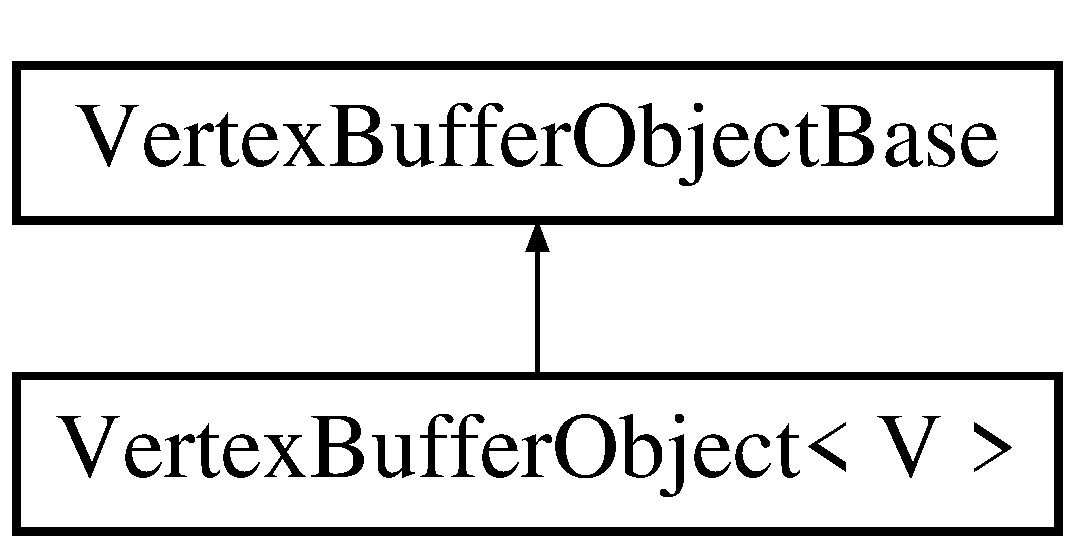
\includegraphics[height=2.000000cm]{class_vertex_buffer_object}
\end{center}
\end{figure}
\subsection*{Public Member Functions}
\begin{DoxyCompactItemize}
\item 
\hyperlink{class_vertex_buffer_object_ac6b700895db0b5f7aaee6e17f6b0db13}{Vertex\+Buffer\+Object} (\hyperlink{class_context}{Context} $\ast$context, const std\+::vector$<$ V $>$ \&vertices)
\begin{DoxyCompactList}\small\item\em Constructor. \end{DoxyCompactList}\item 
virtual \hyperlink{class_vertex_buffer_object_a196fb9f8c90cff926f4bda372b71f23b}{$\sim$\+Vertex\+Buffer\+Object} ()
\begin{DoxyCompactList}\small\item\em Default destructor. \end{DoxyCompactList}\item 
const V \& \hyperlink{class_vertex_buffer_object_a166710d3d7526c9bfb7f99de1b8057a4}{get\+Vertex} (unsigned int index) const 
\begin{DoxyCompactList}\small\item\em Access the vertex at a given offset/index in the buffer. \end{DoxyCompactList}\item 
G\+Lsizei \hyperlink{class_vertex_buffer_object_ab31e996068d871acaa6bb6b5117dd2c3}{get\+Vertex\+Size} () const  override
\begin{DoxyCompactList}\small\item\em Retrieve the size of the individual vertices in this object. \end{DoxyCompactList}\item 
unsigned int \hyperlink{class_vertex_buffer_object_a9c6c36c1711d4fd1d1aae6916c35c9db}{size} () const  override
\begin{DoxyCompactList}\small\item\em Retrieve the size of the vertex buffer. \end{DoxyCompactList}\end{DoxyCompactItemize}
\subsection*{Private Attributes}
\begin{DoxyCompactItemize}
\item 
std\+::vector$<$ V $>$ \hyperlink{class_vertex_buffer_object_aa8ccd2ec2c067c5fff5bb2dded70fcc6}{m\+\_\+\+Vertices}
\begin{DoxyCompactList}\small\item\em C\+P\+U-\/side buffer of vertices. \end{DoxyCompactList}\end{DoxyCompactItemize}


\subsection{Detailed Description}
\subsubsection*{template$<$typename V$>$\\*
class Vertex\+Buffer\+Object$<$ V $>$}

Specialized \hyperlink{class_vertex_buffer_object}{Vertex\+Buffer\+Object} template, for handling generic vertices. 


\begin{DoxyTemplParams}{Template Parameters}
{\em V} & Generic vertex parameter to use for the buffer\\
\hline
\end{DoxyTemplParams}
Whereas the \hyperlink{class_vertex_buffer_object_base}{Vertex\+Buffer\+Object\+Base} allows V\+B\+Os to be represented generically, this class acts as a template for providing vertices to the V\+BO. Consequently, when making a V\+BO, this class template should be used and parameterized with the vertex type used. When using V\+B\+Os in the abstract, consider passing around \hyperlink{class_vertex_buffer_object_base}{Vertex\+Buffer\+Object\+Base} objects instead.

\begin{DoxyPrecond}{Precondition}
A valid Open\+GL context must be present to the program 
\end{DoxyPrecond}
\begin{DoxyAuthor}{Author}
Hayley Hatton 
\end{DoxyAuthor}
\begin{DoxyDate}{Date}
20/02/2016 
\end{DoxyDate}
\begin{DoxySeeAlso}{See also}
\hyperlink{class_vertex_buffer_object_base}{Vertex\+Buffer\+Object\+Base} 
\end{DoxySeeAlso}
\begin{DoxyRefDesc}{Todo}
\item[\hyperlink{todo__todo000007}{Todo}](Hayley\#6\#02/22/16)\+: Handling of dynamic buffers and syncronicity between C\+PU and G\+PU \end{DoxyRefDesc}


Definition at line 25 of file Vertex\+Buffer\+Object.\+h.



\subsection{Constructor \& Destructor Documentation}
\index{Vertex\+Buffer\+Object@{Vertex\+Buffer\+Object}!Vertex\+Buffer\+Object@{Vertex\+Buffer\+Object}}
\index{Vertex\+Buffer\+Object@{Vertex\+Buffer\+Object}!Vertex\+Buffer\+Object@{Vertex\+Buffer\+Object}}
\subsubsection[{\texorpdfstring{Vertex\+Buffer\+Object(\+Context $\ast$context, const std\+::vector$<$ V $>$ \&vertices)}{VertexBufferObject(Context *context, const std::vector< V > &vertices)}}]{\setlength{\rightskip}{0pt plus 5cm}template$<$typename V $>$ {\bf Vertex\+Buffer\+Object}$<$ V $>$\+::{\bf Vertex\+Buffer\+Object} (
\begin{DoxyParamCaption}
\item[{{\bf Context} $\ast$}]{context, }
\item[{const std\+::vector$<$ V $>$ \&}]{vertices}
\end{DoxyParamCaption}
)\hspace{0.3cm}{\ttfamily [inline]}}\hypertarget{class_vertex_buffer_object_ac6b700895db0b5f7aaee6e17f6b0db13}{}\label{class_vertex_buffer_object_ac6b700895db0b5f7aaee6e17f6b0db13}


Constructor. 


\begin{DoxyParams}{Parameters}
{\em context} & Graphics context \\
\hline
{\em vertices} & Array of vertices to initially initialize buffer with \\
\hline
\end{DoxyParams}


Definition at line 33 of file Vertex\+Buffer\+Object.\+h.

\index{Vertex\+Buffer\+Object@{Vertex\+Buffer\+Object}!````~Vertex\+Buffer\+Object@{$\sim$\+Vertex\+Buffer\+Object}}
\index{````~Vertex\+Buffer\+Object@{$\sim$\+Vertex\+Buffer\+Object}!Vertex\+Buffer\+Object@{Vertex\+Buffer\+Object}}
\subsubsection[{\texorpdfstring{$\sim$\+Vertex\+Buffer\+Object()}{~VertexBufferObject()}}]{\setlength{\rightskip}{0pt plus 5cm}template$<$typename V $>$ virtual {\bf Vertex\+Buffer\+Object}$<$ V $>$\+::$\sim${\bf Vertex\+Buffer\+Object} (
\begin{DoxyParamCaption}
{}
\end{DoxyParamCaption}
)\hspace{0.3cm}{\ttfamily [inline]}, {\ttfamily [virtual]}}\hypertarget{class_vertex_buffer_object_a196fb9f8c90cff926f4bda372b71f23b}{}\label{class_vertex_buffer_object_a196fb9f8c90cff926f4bda372b71f23b}


Default destructor. 



Definition at line 54 of file Vertex\+Buffer\+Object.\+h.



\subsection{Member Function Documentation}
\index{Vertex\+Buffer\+Object@{Vertex\+Buffer\+Object}!get\+Vertex@{get\+Vertex}}
\index{get\+Vertex@{get\+Vertex}!Vertex\+Buffer\+Object@{Vertex\+Buffer\+Object}}
\subsubsection[{\texorpdfstring{get\+Vertex(unsigned int index) const }{getVertex(unsigned int index) const }}]{\setlength{\rightskip}{0pt plus 5cm}template$<$typename V $>$ const V\& {\bf Vertex\+Buffer\+Object}$<$ V $>$\+::get\+Vertex (
\begin{DoxyParamCaption}
\item[{unsigned int}]{index}
\end{DoxyParamCaption}
) const\hspace{0.3cm}{\ttfamily [inline]}}\hypertarget{class_vertex_buffer_object_a166710d3d7526c9bfb7f99de1b8057a4}{}\label{class_vertex_buffer_object_a166710d3d7526c9bfb7f99de1b8057a4}


Access the vertex at a given offset/index in the buffer. 


\begin{DoxyParams}{Parameters}
{\em index} & Zero-\/based index in the buffer to access vertex \\
\hline
\end{DoxyParams}
\begin{DoxyReturn}{Returns}
Accessed vertex 
\end{DoxyReturn}


Definition at line 62 of file Vertex\+Buffer\+Object.\+h.



References Vertex\+Buffer\+Object$<$ V $>$\+::m\+\_\+\+Vertices.

\index{Vertex\+Buffer\+Object@{Vertex\+Buffer\+Object}!get\+Vertex\+Size@{get\+Vertex\+Size}}
\index{get\+Vertex\+Size@{get\+Vertex\+Size}!Vertex\+Buffer\+Object@{Vertex\+Buffer\+Object}}
\subsubsection[{\texorpdfstring{get\+Vertex\+Size() const  override}{getVertexSize() const  override}}]{\setlength{\rightskip}{0pt plus 5cm}template$<$typename V $>$ G\+Lsizei {\bf Vertex\+Buffer\+Object}$<$ V $>$\+::get\+Vertex\+Size (
\begin{DoxyParamCaption}
{}
\end{DoxyParamCaption}
) const\hspace{0.3cm}{\ttfamily [inline]}, {\ttfamily [override]}, {\ttfamily [virtual]}}\hypertarget{class_vertex_buffer_object_ab31e996068d871acaa6bb6b5117dd2c3}{}\label{class_vertex_buffer_object_ab31e996068d871acaa6bb6b5117dd2c3}


Retrieve the size of the individual vertices in this object. 

\begin{DoxyReturn}{Returns}
Size of a vertex, in G\+L-\/casted format 
\end{DoxyReturn}


Implements \hyperlink{class_vertex_buffer_object_base_aff976ee272a27c43b95ee0c6cb0a7506}{Vertex\+Buffer\+Object\+Base}.



Definition at line 68 of file Vertex\+Buffer\+Object.\+h.

\index{Vertex\+Buffer\+Object@{Vertex\+Buffer\+Object}!size@{size}}
\index{size@{size}!Vertex\+Buffer\+Object@{Vertex\+Buffer\+Object}}
\subsubsection[{\texorpdfstring{size() const  override}{size() const  override}}]{\setlength{\rightskip}{0pt plus 5cm}template$<$typename V $>$ unsigned int {\bf Vertex\+Buffer\+Object}$<$ V $>$\+::size (
\begin{DoxyParamCaption}
{}
\end{DoxyParamCaption}
) const\hspace{0.3cm}{\ttfamily [inline]}, {\ttfamily [override]}, {\ttfamily [virtual]}}\hypertarget{class_vertex_buffer_object_a9c6c36c1711d4fd1d1aae6916c35c9db}{}\label{class_vertex_buffer_object_a9c6c36c1711d4fd1d1aae6916c35c9db}


Retrieve the size of the vertex buffer. 

\begin{DoxyReturn}{Returns}
Number of vertices in the C\+P\+U-\/side buffer 
\end{DoxyReturn}


Implements \hyperlink{class_vertex_buffer_object_base_ab11e9eae754a9b12012242042d9637f0}{Vertex\+Buffer\+Object\+Base}.



Definition at line 74 of file Vertex\+Buffer\+Object.\+h.



References Vertex\+Buffer\+Object$<$ V $>$\+::m\+\_\+\+Vertices.



\subsection{Member Data Documentation}
\index{Vertex\+Buffer\+Object@{Vertex\+Buffer\+Object}!m\+\_\+\+Vertices@{m\+\_\+\+Vertices}}
\index{m\+\_\+\+Vertices@{m\+\_\+\+Vertices}!Vertex\+Buffer\+Object@{Vertex\+Buffer\+Object}}
\subsubsection[{\texorpdfstring{m\+\_\+\+Vertices}{m_Vertices}}]{\setlength{\rightskip}{0pt plus 5cm}template$<$typename V $>$ std\+::vector$<$V$>$ {\bf Vertex\+Buffer\+Object}$<$ V $>$\+::m\+\_\+\+Vertices\hspace{0.3cm}{\ttfamily [private]}}\hypertarget{class_vertex_buffer_object_aa8ccd2ec2c067c5fff5bb2dded70fcc6}{}\label{class_vertex_buffer_object_aa8ccd2ec2c067c5fff5bb2dded70fcc6}


C\+P\+U-\/side buffer of vertices. 



Definition at line 77 of file Vertex\+Buffer\+Object.\+h.



Referenced by Vertex\+Buffer\+Object$<$ V $>$\+::get\+Vertex(), and Vertex\+Buffer\+Object$<$ V $>$\+::size().



The documentation for this class was generated from the following file\+:\begin{DoxyCompactItemize}
\item 
Lunar\+Drift/engine/graphics/buffers/\hyperlink{_vertex_buffer_object_8h}{Vertex\+Buffer\+Object.\+h}\end{DoxyCompactItemize}

\hypertarget{class_vertex_buffer_object_base}{}\section{Vertex\+Buffer\+Object\+Base Class Reference}
\label{class_vertex_buffer_object_base}\index{Vertex\+Buffer\+Object\+Base@{Vertex\+Buffer\+Object\+Base}}


Abstract base class for specialized Vertex\+Buffer\+Objects.  




{\ttfamily \#include $<$Vertex\+Buffer\+Object\+Base.\+h$>$}

Inheritance diagram for Vertex\+Buffer\+Object\+Base\+:\begin{figure}[H]
\begin{center}
\leavevmode
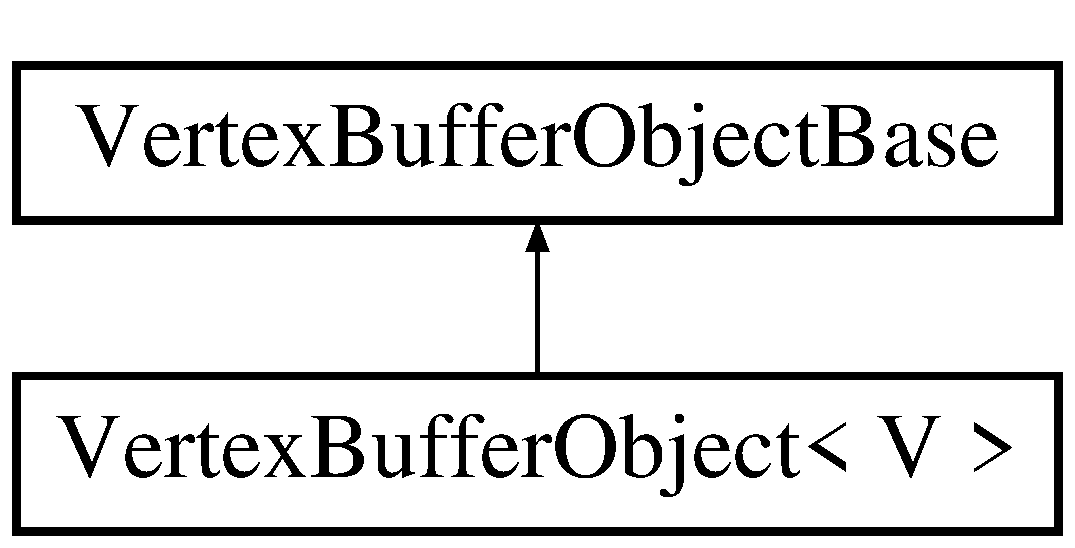
\includegraphics[height=2.000000cm]{class_vertex_buffer_object_base}
\end{center}
\end{figure}
\subsection*{Public Member Functions}
\begin{DoxyCompactItemize}
\item 
\hyperlink{class_vertex_buffer_object_base_ab08c82b0b8b58d6dc0d7aa0c218eed98}{Vertex\+Buffer\+Object\+Base} (\hyperlink{class_context}{Context} $\ast$context)
\begin{DoxyCompactList}\small\item\em Default constructor. \end{DoxyCompactList}\item 
virtual \hyperlink{class_vertex_buffer_object_base_acc84ed51a8fa9e78e5692e5695ce2d17}{$\sim$\+Vertex\+Buffer\+Object\+Base} ()
\begin{DoxyCompactList}\small\item\em Default destructor. \end{DoxyCompactList}\item 
virtual G\+Lsizei \hyperlink{class_vertex_buffer_object_base_aff976ee272a27c43b95ee0c6cb0a7506}{get\+Vertex\+Size} () const  =0
\begin{DoxyCompactList}\small\item\em Retrieve the size of the individual vertices in this object. \end{DoxyCompactList}\item 
virtual unsigned int \hyperlink{class_vertex_buffer_object_base_ab11e9eae754a9b12012242042d9637f0}{size} () const  =0
\begin{DoxyCompactList}\small\item\em Retrieve the size of the vertex buffer. \end{DoxyCompactList}\item 
void \hyperlink{class_vertex_buffer_object_base_a364a7e5955125bf8fda040109e9734e4}{bind} (\hyperlink{class_context}{Context} $\ast$context)
\begin{DoxyCompactList}\small\item\em Bind the V\+BO to the Open\+GL state pipeline. \end{DoxyCompactList}\end{DoxyCompactItemize}
\subsection*{Private Attributes}
\begin{DoxyCompactItemize}
\item 
G\+Luint \hyperlink{class_vertex_buffer_object_base_a93987eea648e4c871c404716e1af8b8d}{m\+\_\+\+V\+BO}
\begin{DoxyCompactList}\small\item\em Open\+G\+L-\/provided V\+BO handle. \end{DoxyCompactList}\end{DoxyCompactItemize}


\subsection{Detailed Description}
Abstract base class for specialized Vertex\+Buffer\+Objects. 

This class represents V\+B\+Os in the abstract, managing their representation in Open\+GL in a way that\textquotesingle{}s agnostic with regards to the data stored in the V\+BO themselves. In most cases, this class will only be used when passing around V\+B\+Os as an abstract concept; to work with V\+B\+Os, one should use the \hyperlink{class_vertex_buffer_object}{Vertex\+Buffer\+Object} class template with the vertex type specified.

\begin{DoxyPrecond}{Precondition}
A valid Open\+GL context must be present to the program 
\end{DoxyPrecond}
\begin{DoxyAuthor}{Author}
Hayley Hatton 
\end{DoxyAuthor}
\begin{DoxyDate}{Date}
20/02/2016 
\end{DoxyDate}
\begin{DoxySeeAlso}{See also}
\hyperlink{class_vertex_buffer_object}{Vertex\+Buffer\+Object} 
\end{DoxySeeAlso}
\begin{DoxyRefDesc}{Todo}
\item[\hyperlink{todo__todo000008}{Todo}](Hayley\#6\#02/22/16)\+: Handling of dynamic buffers and syncronicity between C\+PU and G\+PU \end{DoxyRefDesc}


Definition at line 20 of file Vertex\+Buffer\+Object\+Base.\+h.



\subsection{Constructor \& Destructor Documentation}
\index{Vertex\+Buffer\+Object\+Base@{Vertex\+Buffer\+Object\+Base}!Vertex\+Buffer\+Object\+Base@{Vertex\+Buffer\+Object\+Base}}
\index{Vertex\+Buffer\+Object\+Base@{Vertex\+Buffer\+Object\+Base}!Vertex\+Buffer\+Object\+Base@{Vertex\+Buffer\+Object\+Base}}
\subsubsection[{\texorpdfstring{Vertex\+Buffer\+Object\+Base(\+Context $\ast$context)}{VertexBufferObjectBase(Context *context)}}]{\setlength{\rightskip}{0pt plus 5cm}Vertex\+Buffer\+Object\+Base\+::\+Vertex\+Buffer\+Object\+Base (
\begin{DoxyParamCaption}
\item[{{\bf Context} $\ast$}]{context}
\end{DoxyParamCaption}
)}\hypertarget{class_vertex_buffer_object_base_ab08c82b0b8b58d6dc0d7aa0c218eed98}{}\label{class_vertex_buffer_object_base_ab08c82b0b8b58d6dc0d7aa0c218eed98}


Default constructor. 


\begin{DoxyParams}{Parameters}
{\em context} & Graphics context \\
\hline
\end{DoxyParams}


Definition at line 5 of file Vertex\+Buffer\+Object\+Base.\+cpp.



References bind(), and m\+\_\+\+V\+BO.

\index{Vertex\+Buffer\+Object\+Base@{Vertex\+Buffer\+Object\+Base}!````~Vertex\+Buffer\+Object\+Base@{$\sim$\+Vertex\+Buffer\+Object\+Base}}
\index{````~Vertex\+Buffer\+Object\+Base@{$\sim$\+Vertex\+Buffer\+Object\+Base}!Vertex\+Buffer\+Object\+Base@{Vertex\+Buffer\+Object\+Base}}
\subsubsection[{\texorpdfstring{$\sim$\+Vertex\+Buffer\+Object\+Base()}{~VertexBufferObjectBase()}}]{\setlength{\rightskip}{0pt plus 5cm}Vertex\+Buffer\+Object\+Base\+::$\sim$\+Vertex\+Buffer\+Object\+Base (
\begin{DoxyParamCaption}
{}
\end{DoxyParamCaption}
)\hspace{0.3cm}{\ttfamily [virtual]}}\hypertarget{class_vertex_buffer_object_base_acc84ed51a8fa9e78e5692e5695ce2d17}{}\label{class_vertex_buffer_object_base_acc84ed51a8fa9e78e5692e5695ce2d17}


Default destructor. 



Definition at line 21 of file Vertex\+Buffer\+Object\+Base.\+cpp.



References m\+\_\+\+V\+BO.



\subsection{Member Function Documentation}
\index{Vertex\+Buffer\+Object\+Base@{Vertex\+Buffer\+Object\+Base}!bind@{bind}}
\index{bind@{bind}!Vertex\+Buffer\+Object\+Base@{Vertex\+Buffer\+Object\+Base}}
\subsubsection[{\texorpdfstring{bind(\+Context $\ast$context)}{bind(Context *context)}}]{\setlength{\rightskip}{0pt plus 5cm}void Vertex\+Buffer\+Object\+Base\+::bind (
\begin{DoxyParamCaption}
\item[{{\bf Context} $\ast$}]{context}
\end{DoxyParamCaption}
)}\hypertarget{class_vertex_buffer_object_base_a364a7e5955125bf8fda040109e9734e4}{}\label{class_vertex_buffer_object_base_a364a7e5955125bf8fda040109e9734e4}


Bind the V\+BO to the Open\+GL state pipeline. 


\begin{DoxyParams}{Parameters}
{\em context} & Graphics context \\
\hline
\end{DoxyParams}


Definition at line 27 of file Vertex\+Buffer\+Object\+Base.\+cpp.



References m\+\_\+\+V\+BO.



Referenced by Vertex\+Buffer\+Object\+Base().

\index{Vertex\+Buffer\+Object\+Base@{Vertex\+Buffer\+Object\+Base}!get\+Vertex\+Size@{get\+Vertex\+Size}}
\index{get\+Vertex\+Size@{get\+Vertex\+Size}!Vertex\+Buffer\+Object\+Base@{Vertex\+Buffer\+Object\+Base}}
\subsubsection[{\texorpdfstring{get\+Vertex\+Size() const  =0}{getVertexSize() const  =0}}]{\setlength{\rightskip}{0pt plus 5cm}virtual G\+Lsizei Vertex\+Buffer\+Object\+Base\+::get\+Vertex\+Size (
\begin{DoxyParamCaption}
{}
\end{DoxyParamCaption}
) const\hspace{0.3cm}{\ttfamily [pure virtual]}}\hypertarget{class_vertex_buffer_object_base_aff976ee272a27c43b95ee0c6cb0a7506}{}\label{class_vertex_buffer_object_base_aff976ee272a27c43b95ee0c6cb0a7506}


Retrieve the size of the individual vertices in this object. 

\begin{DoxyReturn}{Returns}
Size of a vertex, in G\+L-\/casted format 
\end{DoxyReturn}


Implemented in \hyperlink{class_vertex_buffer_object_ab31e996068d871acaa6bb6b5117dd2c3}{Vertex\+Buffer\+Object$<$ V $>$}.

\index{Vertex\+Buffer\+Object\+Base@{Vertex\+Buffer\+Object\+Base}!size@{size}}
\index{size@{size}!Vertex\+Buffer\+Object\+Base@{Vertex\+Buffer\+Object\+Base}}
\subsubsection[{\texorpdfstring{size() const  =0}{size() const  =0}}]{\setlength{\rightskip}{0pt plus 5cm}virtual unsigned int Vertex\+Buffer\+Object\+Base\+::size (
\begin{DoxyParamCaption}
{}
\end{DoxyParamCaption}
) const\hspace{0.3cm}{\ttfamily [pure virtual]}}\hypertarget{class_vertex_buffer_object_base_ab11e9eae754a9b12012242042d9637f0}{}\label{class_vertex_buffer_object_base_ab11e9eae754a9b12012242042d9637f0}


Retrieve the size of the vertex buffer. 

\begin{DoxyReturn}{Returns}
Number of vertices in the C\+P\+U-\/side buffer 
\end{DoxyReturn}


Implemented in \hyperlink{class_vertex_buffer_object_a9c6c36c1711d4fd1d1aae6916c35c9db}{Vertex\+Buffer\+Object$<$ V $>$}.



\subsection{Member Data Documentation}
\index{Vertex\+Buffer\+Object\+Base@{Vertex\+Buffer\+Object\+Base}!m\+\_\+\+V\+BO@{m\+\_\+\+V\+BO}}
\index{m\+\_\+\+V\+BO@{m\+\_\+\+V\+BO}!Vertex\+Buffer\+Object\+Base@{Vertex\+Buffer\+Object\+Base}}
\subsubsection[{\texorpdfstring{m\+\_\+\+V\+BO}{m_VBO}}]{\setlength{\rightskip}{0pt plus 5cm}G\+Luint Vertex\+Buffer\+Object\+Base\+::m\+\_\+\+V\+BO\hspace{0.3cm}{\ttfamily [private]}}\hypertarget{class_vertex_buffer_object_base_a93987eea648e4c871c404716e1af8b8d}{}\label{class_vertex_buffer_object_base_a93987eea648e4c871c404716e1af8b8d}


Open\+G\+L-\/provided V\+BO handle. 



Definition at line 53 of file Vertex\+Buffer\+Object\+Base.\+h.



Referenced by bind(), Vertex\+Buffer\+Object\+Base(), and $\sim$\+Vertex\+Buffer\+Object\+Base().



The documentation for this class was generated from the following files\+:\begin{DoxyCompactItemize}
\item 
Lunar\+Drift/engine/graphics/buffers/\hyperlink{_vertex_buffer_object_base_8h}{Vertex\+Buffer\+Object\+Base.\+h}\item 
Lunar\+Drift/engine/graphics/buffers/\hyperlink{_vertex_buffer_object_base_8cpp}{Vertex\+Buffer\+Object\+Base.\+cpp}\end{DoxyCompactItemize}

\hypertarget{struct_window_p_c_1_1_w_i_n32___e_v_e_n_t}{}\section{Window\+PC\+:\+:W\+I\+N32\+\_\+\+E\+V\+E\+NT Struct Reference}
\label{struct_window_p_c_1_1_w_i_n32___e_v_e_n_t}\index{Window\+P\+C\+::\+W\+I\+N32\+\_\+\+E\+V\+E\+NT@{Window\+P\+C\+::\+W\+I\+N32\+\_\+\+E\+V\+E\+NT}}
\subsection*{Public Attributes}
\begin{DoxyCompactItemize}
\item 
U\+I\+NT \hyperlink{struct_window_p_c_1_1_w_i_n32___e_v_e_n_t_a2e5b34b5b59137ceedfcbf252695f146}{message}
\item 
W\+P\+A\+R\+AM \hyperlink{struct_window_p_c_1_1_w_i_n32___e_v_e_n_t_ac895aec4d3d1953b85923f0a5da45004}{w\+Param}
\item 
L\+P\+A\+R\+AM \hyperlink{struct_window_p_c_1_1_w_i_n32___e_v_e_n_t_a13a17a5f5efbfb902556ab01a3f825f6}{l\+Param}
\end{DoxyCompactItemize}


\subsection{Detailed Description}


Definition at line 81 of file Window\+P\+C.\+h.



\subsection{Member Data Documentation}
\index{Window\+P\+C\+::\+W\+I\+N32\+\_\+\+E\+V\+E\+NT@{Window\+P\+C\+::\+W\+I\+N32\+\_\+\+E\+V\+E\+NT}!l\+Param@{l\+Param}}
\index{l\+Param@{l\+Param}!Window\+P\+C\+::\+W\+I\+N32\+\_\+\+E\+V\+E\+NT@{Window\+P\+C\+::\+W\+I\+N32\+\_\+\+E\+V\+E\+NT}}
\subsubsection[{\texorpdfstring{l\+Param}{lParam}}]{\setlength{\rightskip}{0pt plus 5cm}L\+P\+A\+R\+AM Window\+P\+C\+::\+W\+I\+N32\+\_\+\+E\+V\+E\+N\+T\+::l\+Param}\hypertarget{struct_window_p_c_1_1_w_i_n32___e_v_e_n_t_a13a17a5f5efbfb902556ab01a3f825f6}{}\label{struct_window_p_c_1_1_w_i_n32___e_v_e_n_t_a13a17a5f5efbfb902556ab01a3f825f6}


Definition at line 85 of file Window\+P\+C.\+h.

\index{Window\+P\+C\+::\+W\+I\+N32\+\_\+\+E\+V\+E\+NT@{Window\+P\+C\+::\+W\+I\+N32\+\_\+\+E\+V\+E\+NT}!message@{message}}
\index{message@{message}!Window\+P\+C\+::\+W\+I\+N32\+\_\+\+E\+V\+E\+NT@{Window\+P\+C\+::\+W\+I\+N32\+\_\+\+E\+V\+E\+NT}}
\subsubsection[{\texorpdfstring{message}{message}}]{\setlength{\rightskip}{0pt plus 5cm}U\+I\+NT Window\+P\+C\+::\+W\+I\+N32\+\_\+\+E\+V\+E\+N\+T\+::message}\hypertarget{struct_window_p_c_1_1_w_i_n32___e_v_e_n_t_a2e5b34b5b59137ceedfcbf252695f146}{}\label{struct_window_p_c_1_1_w_i_n32___e_v_e_n_t_a2e5b34b5b59137ceedfcbf252695f146}


Definition at line 83 of file Window\+P\+C.\+h.



Referenced by Window\+P\+C\+::handle\+Win32\+Event\+Queue().

\index{Window\+P\+C\+::\+W\+I\+N32\+\_\+\+E\+V\+E\+NT@{Window\+P\+C\+::\+W\+I\+N32\+\_\+\+E\+V\+E\+NT}!w\+Param@{w\+Param}}
\index{w\+Param@{w\+Param}!Window\+P\+C\+::\+W\+I\+N32\+\_\+\+E\+V\+E\+NT@{Window\+P\+C\+::\+W\+I\+N32\+\_\+\+E\+V\+E\+NT}}
\subsubsection[{\texorpdfstring{w\+Param}{wParam}}]{\setlength{\rightskip}{0pt plus 5cm}W\+P\+A\+R\+AM Window\+P\+C\+::\+W\+I\+N32\+\_\+\+E\+V\+E\+N\+T\+::w\+Param}\hypertarget{struct_window_p_c_1_1_w_i_n32___e_v_e_n_t_ac895aec4d3d1953b85923f0a5da45004}{}\label{struct_window_p_c_1_1_w_i_n32___e_v_e_n_t_ac895aec4d3d1953b85923f0a5da45004}


Definition at line 84 of file Window\+P\+C.\+h.



Referenced by Window\+P\+C\+::handle\+Win32\+Event\+Queue().



The documentation for this struct was generated from the following file\+:\begin{DoxyCompactItemize}
\item 
Lunar\+Drift/engine/containers/\hyperlink{_window_p_c_8h}{Window\+P\+C.\+h}\end{DoxyCompactItemize}

\hypertarget{class_window}{}\section{Window Class Reference}
\label{class_window}\index{Window@{Window}}


Abstract window container, for bridging the system to the program.  




{\ttfamily \#include $<$Window.\+h$>$}

Inheritance diagram for Window\+:\begin{figure}[H]
\begin{center}
\leavevmode
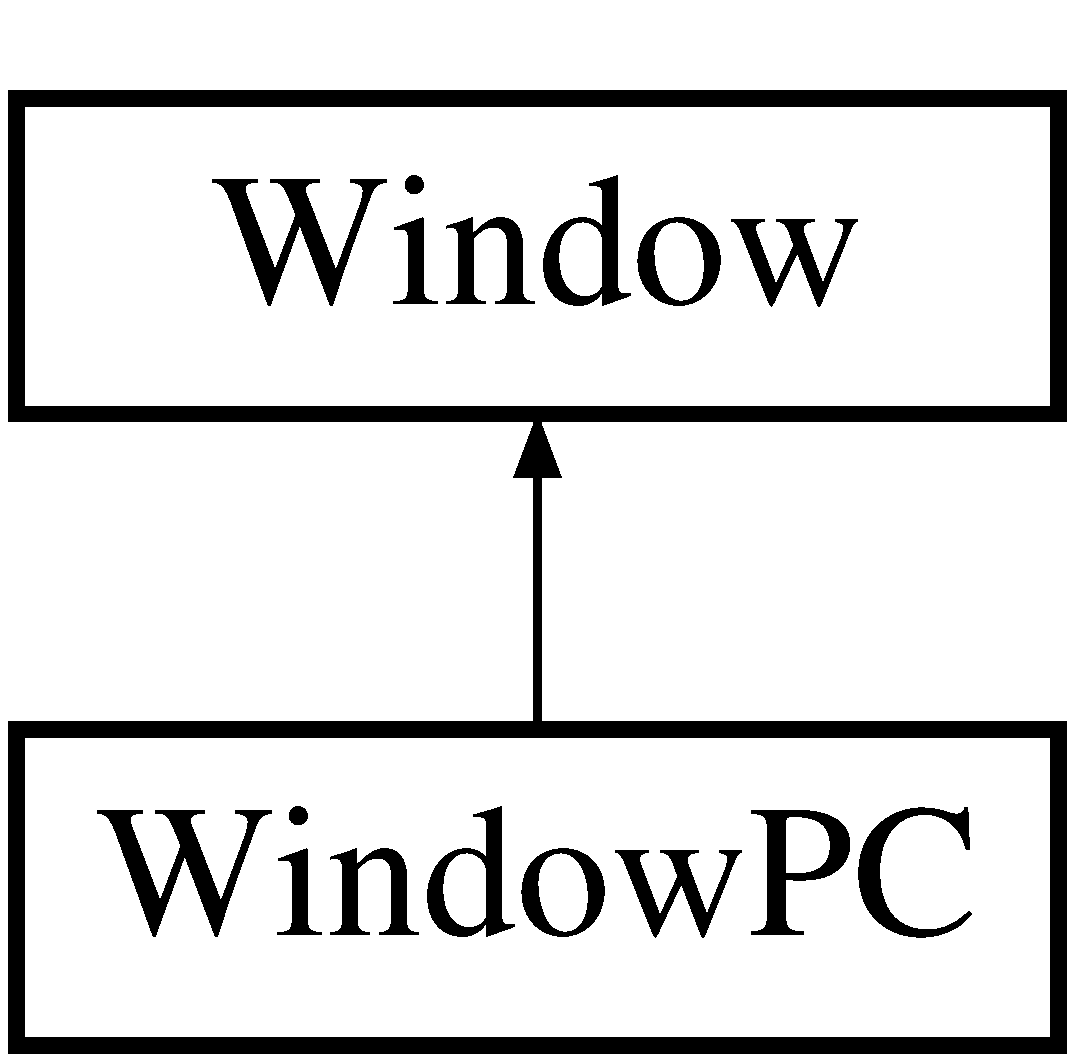
\includegraphics[height=2.000000cm]{class_window}
\end{center}
\end{figure}
\subsection*{Public Member Functions}
\begin{DoxyCompactItemize}
\item 
\hyperlink{class_window_a74e6087da23d3c24e9fac0245e5ec92c}{Window} ()
\begin{DoxyCompactList}\small\item\em Default constructor. \end{DoxyCompactList}\item 
virtual \hyperlink{class_window_a245d821e6016fa1f6970ccbbedd635f6}{$\sim$\+Window} ()
\begin{DoxyCompactList}\small\item\em Default destructor. \end{DoxyCompactList}\item 
virtual \hyperlink{_window_8h_ae189a3c432aa37137a55df8c91c579ed}{Exit\+Status} \hyperlink{class_window_ad98ff66251be5270bdf3fe2e731dec0b}{run} (std\+::unique\+\_\+ptr$<$ \hyperlink{class_program}{Program} $>$ program)=0
\begin{DoxyCompactList}\small\item\em Main execution point for the window. \end{DoxyCompactList}\end{DoxyCompactItemize}
\subsection*{Protected Member Functions}
\begin{DoxyCompactItemize}
\item 
\hyperlink{class_program}{Program} $\ast$ \hyperlink{class_window_afbdf70548ae7b866e0b535cef8282c62}{get\+Program} ()
\begin{DoxyCompactList}\small\item\em Access the currently-\/executing program instance. \end{DoxyCompactList}\item 
std\+::string \hyperlink{class_window_a0d02e0859c746105a40bf8b60584908d}{get\+G\+P\+U\+Name} () const 
\end{DoxyCompactItemize}
\subsection*{Private Attributes}
\begin{DoxyCompactItemize}
\item 
\hyperlink{class_program}{Program} $\ast$ \hyperlink{class_window_afcae84b6b4fbc790bae19b794809f98b}{m\+\_\+\+Program}
\begin{DoxyCompactList}\small\item\em Pointer to program class. \end{DoxyCompactList}\end{DoxyCompactItemize}


\subsection{Detailed Description}
Abstract window container, for bridging the system to the program. 

\begin{DoxyAuthor}{Author}
Hayley Hatton 
\end{DoxyAuthor}
\begin{DoxyDate}{Date}
06/03/2016 
\end{DoxyDate}


Definition at line 19 of file Window.\+h.



\subsection{Constructor \& Destructor Documentation}
\index{Window@{Window}!Window@{Window}}
\index{Window@{Window}!Window@{Window}}
\subsubsection[{\texorpdfstring{Window()}{Window()}}]{\setlength{\rightskip}{0pt plus 5cm}Window\+::\+Window (
\begin{DoxyParamCaption}
{}
\end{DoxyParamCaption}
)}\hypertarget{class_window_a74e6087da23d3c24e9fac0245e5ec92c}{}\label{class_window_a74e6087da23d3c24e9fac0245e5ec92c}


Default constructor. 



Definition at line 3 of file Window.\+cpp.

\index{Window@{Window}!````~Window@{$\sim$\+Window}}
\index{````~Window@{$\sim$\+Window}!Window@{Window}}
\subsubsection[{\texorpdfstring{$\sim$\+Window()}{~Window()}}]{\setlength{\rightskip}{0pt plus 5cm}Window\+::$\sim$\+Window (
\begin{DoxyParamCaption}
{}
\end{DoxyParamCaption}
)\hspace{0.3cm}{\ttfamily [virtual]}}\hypertarget{class_window_a245d821e6016fa1f6970ccbbedd635f6}{}\label{class_window_a245d821e6016fa1f6970ccbbedd635f6}


Default destructor. 



Definition at line 8 of file Window.\+cpp.



\subsection{Member Function Documentation}
\index{Window@{Window}!get\+G\+P\+U\+Name@{get\+G\+P\+U\+Name}}
\index{get\+G\+P\+U\+Name@{get\+G\+P\+U\+Name}!Window@{Window}}
\subsubsection[{\texorpdfstring{get\+G\+P\+U\+Name() const }{getGPUName() const }}]{\setlength{\rightskip}{0pt plus 5cm}std\+::string Window\+::get\+G\+P\+U\+Name (
\begin{DoxyParamCaption}
{}
\end{DoxyParamCaption}
) const\hspace{0.3cm}{\ttfamily [protected]}}\hypertarget{class_window_a0d02e0859c746105a40bf8b60584908d}{}\label{class_window_a0d02e0859c746105a40bf8b60584908d}


Definition at line 20 of file Window.\+cpp.



Referenced by Window\+P\+C\+::\+Window\+P\+C().

\index{Window@{Window}!get\+Program@{get\+Program}}
\index{get\+Program@{get\+Program}!Window@{Window}}
\subsubsection[{\texorpdfstring{get\+Program()}{getProgram()}}]{\setlength{\rightskip}{0pt plus 5cm}{\bf Program}$\ast$ Window\+::get\+Program (
\begin{DoxyParamCaption}
{}
\end{DoxyParamCaption}
)\hspace{0.3cm}{\ttfamily [inline]}, {\ttfamily [protected]}}\hypertarget{class_window_afbdf70548ae7b866e0b535cef8282c62}{}\label{class_window_afbdf70548ae7b866e0b535cef8282c62}


Access the currently-\/executing program instance. 

\begin{DoxyReturn}{Returns}
Pointer to the currently-\/executing program; nullptr if none 
\end{DoxyReturn}


Definition at line 40 of file Window.\+h.

\index{Window@{Window}!run@{run}}
\index{run@{run}!Window@{Window}}
\subsubsection[{\texorpdfstring{run(std\+::unique\+\_\+ptr$<$ Program $>$ program)=0}{run(std::unique_ptr< Program > program)=0}}]{\setlength{\rightskip}{0pt plus 5cm}virtual {\bf Exit\+Status} Window\+::run (
\begin{DoxyParamCaption}
\item[{std\+::unique\+\_\+ptr$<$ {\bf Program} $>$}]{program}
\end{DoxyParamCaption}
)\hspace{0.3cm}{\ttfamily [pure virtual]}}\hypertarget{class_window_ad98ff66251be5270bdf3fe2e731dec0b}{}\label{class_window_ad98ff66251be5270bdf3fe2e731dec0b}


Main execution point for the window. 


\begin{DoxyParams}{Parameters}
{\em program} & Pointer to program to execute \\
\hline
\end{DoxyParams}
\begin{DoxyReturn}{Returns}
State indicator to inform the desktop whether execution succeeded 
\end{DoxyReturn}


Implemented in \hyperlink{class_window_p_c_a37f3734410e8a9d99b5de80de7c14bf5}{Window\+PC}.



\subsection{Member Data Documentation}
\index{Window@{Window}!m\+\_\+\+Program@{m\+\_\+\+Program}}
\index{m\+\_\+\+Program@{m\+\_\+\+Program}!Window@{Window}}
\subsubsection[{\texorpdfstring{m\+\_\+\+Program}{m_Program}}]{\setlength{\rightskip}{0pt plus 5cm}{\bf Program}$\ast$ Window\+::m\+\_\+\+Program\hspace{0.3cm}{\ttfamily [private]}}\hypertarget{class_window_afcae84b6b4fbc790bae19b794809f98b}{}\label{class_window_afcae84b6b4fbc790bae19b794809f98b}


Pointer to program class. 



Definition at line 45 of file Window.\+h.



The documentation for this class was generated from the following files\+:\begin{DoxyCompactItemize}
\item 
Lunar\+Drift/engine/containers/\hyperlink{_window_8h}{Window.\+h}\item 
Lunar\+Drift/engine/containers/\hyperlink{_window_8cpp}{Window.\+cpp}\end{DoxyCompactItemize}

\hypertarget{class_window_p_c}{}\section{Window\+PC Class Reference}
\label{class_window_p_c}\index{Window\+PC@{Window\+PC}}


\hyperlink{class_window}{Window} class for use on Windows desktop P\+Cs.  




{\ttfamily \#include $<$Window\+P\+C.\+h$>$}

Inheritance diagram for Window\+PC\+:\begin{figure}[H]
\begin{center}
\leavevmode
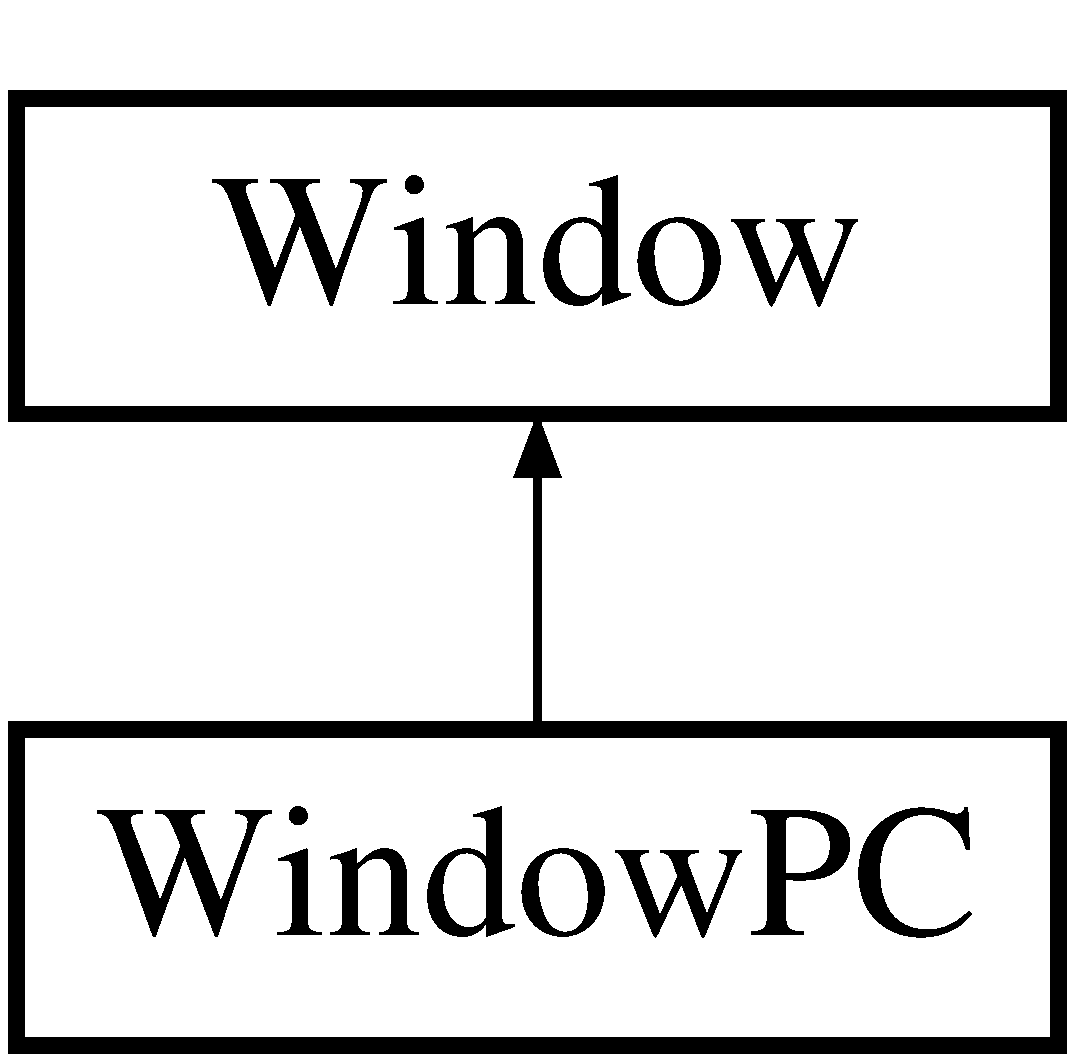
\includegraphics[height=2.000000cm]{class_window_p_c}
\end{center}
\end{figure}
\subsection*{Classes}
\begin{DoxyCompactItemize}
\item 
struct \hyperlink{struct_window_p_c_1_1_w_i_n32___e_v_e_n_t}{W\+I\+N32\+\_\+\+E\+V\+E\+NT}
\end{DoxyCompactItemize}
\subsection*{Public Member Functions}
\begin{DoxyCompactItemize}
\item 
\hyperlink{class_window_p_c_a96a4c01f2eaa2a07d3ad67e993c241c8}{Window\+PC} (const std\+::string \&title, H\+I\+N\+S\+T\+A\+N\+CE h\+Instance, L\+P\+S\+TR lp\+Cmd\+Line, int n\+Cmd\+Show, unsigned int width, unsigned int height)
\begin{DoxyCompactList}\small\item\em Default constructor; sets up the environment. \end{DoxyCompactList}\item 
virtual \hyperlink{class_window_p_c_a0524b2e9b75c81207d4874809f687110}{$\sim$\+Window\+PC} ()
\begin{DoxyCompactList}\small\item\em Default destructor. \end{DoxyCompactList}\item 
\hyperlink{class_context}{Context} $\ast$ \hyperlink{class_window_p_c_af211b371f3cbe8cda20dbeb47ad9a359}{get\+Context} ()
\begin{DoxyCompactList}\small\item\em Access the underlying graphics context. \end{DoxyCompactList}\item 
\hyperlink{_window_8h_ae189a3c432aa37137a55df8c91c579ed}{Exit\+Status} \hyperlink{class_window_p_c_a37f3734410e8a9d99b5de80de7c14bf5}{run} (std\+::unique\+\_\+ptr$<$ \hyperlink{class_program}{Program} $>$ program) override
\begin{DoxyCompactList}\small\item\em Running environment, with the final return status. \end{DoxyCompactList}\item 
void \hyperlink{class_window_p_c_ae12f24716fa0b959e65580aead8f3fc9}{simulation\+Thread} (\hyperlink{class_program}{Program} $\ast$program)
\begin{DoxyCompactList}\small\item\em Simulation thread function. \end{DoxyCompactList}\item 
void \hyperlink{class_window_p_c_a329f37bb75b5ed1c5303fde8b7cef63f}{rendering\+Thread} (\hyperlink{class_context}{Context} $\ast$context, \hyperlink{class_program}{Program} $\ast$program)
\begin{DoxyCompactList}\small\item\em Rendering thread function. \end{DoxyCompactList}\end{DoxyCompactItemize}
\subsection*{Static Public Member Functions}
\begin{DoxyCompactItemize}
\item 
static L\+R\+E\+S\+U\+LT C\+A\+L\+L\+B\+A\+CK \hyperlink{class_window_p_c_a135d3ecba5245fd810c2e3e3d9cf8cf9}{Window\+Proc} (H\+W\+ND h\+Wnd, U\+I\+NT message, W\+P\+A\+R\+AM w\+Param, L\+P\+A\+R\+AM l\+Param)
\end{DoxyCompactItemize}
\subsection*{Protected Member Functions}
\begin{DoxyCompactItemize}
\item 
void \hyperlink{class_window_p_c_a50f059f9690a597769035c9d1a81e994}{pre\+Frame} (\hyperlink{class_context}{Context} $\ast$context)
\begin{DoxyCompactList}\small\item\em Do anything that needs to be done immediately before rendering. \end{DoxyCompactList}\item 
void \hyperlink{class_window_p_c_aa910bf9e32d41941f48eec5f2872ee80}{post\+Frame} (\hyperlink{class_context}{Context} $\ast$context)
\begin{DoxyCompactList}\small\item\em Do anything that needs to be done immediately after rendering A prime example of this is the swapping of back-\/buffer to the display. \end{DoxyCompactList}\end{DoxyCompactItemize}
\subsection*{Private Member Functions}
\begin{DoxyCompactItemize}
\item 
void \hyperlink{class_window_p_c_a18c8c102251f65235f83b733d248ed15}{post\+Win32\+Event\+To\+Queue} (\hyperlink{struct_window_p_c_1_1_w_i_n32___e_v_e_n_t}{W\+I\+N32\+\_\+\+E\+V\+E\+NT} \&wievent)
\item 
void \hyperlink{class_window_p_c_abd03ac9a2e3e653a3762374b2ed6f250}{handle\+Win32\+Event\+Queue} ()
\item 
void \hyperlink{class_window_p_c_ae90444398408f0b3e2248a1bcaf1f87f}{temp\+Window\+Stuff} (const std\+::string \&title, H\+I\+N\+S\+T\+A\+N\+CE h\+Instance)
\item 
void \hyperlink{class_window_p_c_aa3d6fac4c045f2eaf5caa0a73bc8f8b5}{init\+GL} (H\+W\+ND h\+Wnd, bool v\+Sync=false)
\item 
H\+W\+ND \hyperlink{class_window_p_c_abefc415a2ebea795117000822c1d4c6f}{create\+Window} (const std\+::string \&title, unsigned int width, unsigned int height, bool show, H\+I\+N\+S\+T\+A\+N\+CE h\+Instance)
\item 
H\+W\+ND \hyperlink{class_window_p_c_aafe0e02b17a2e11418d9957e7f2aaae9}{create\+Window} (const std\+::string \&title, H\+I\+N\+S\+T\+A\+N\+CE h\+Instance)
\item 
void \hyperlink{class_window_p_c_a2f3d974dc86bee64deeec258ec0bf548}{destroy\+Window} (H\+W\+ND h\+Wnd)
\end{DoxyCompactItemize}
\subsection*{Private Attributes}
\begin{DoxyCompactItemize}
\item 
H\+W\+ND \hyperlink{class_window_p_c_a49b7d0fb393f4316e78dc753946fd5f9}{m\+\_\+\+H\+Wnd}
\item 
H\+DC \hyperlink{class_window_p_c_af536c182db956b1e87d6f5ba20beb172}{m\+\_\+\+H\+DC}
\item 
H\+G\+L\+RC \hyperlink{class_window_p_c_a5818491db2c9d38e13d4022cf2451889}{m\+\_\+\+H\+RC}
\item 
std\+::queue$<$ \hyperlink{struct_window_p_c_1_1_w_i_n32___e_v_e_n_t}{W\+I\+N32\+\_\+\+E\+V\+E\+NT} $>$ \hyperlink{class_window_p_c_aae73501b77c9ab90594bd9dde22e7416}{m\+\_\+\+Event\+Queue}
\item 
std\+::mutex \hyperlink{class_window_p_c_a1a277bf91c4c052094e7d6ec2005a2c1}{m\+\_\+\+Event\+Mtx}
\begin{DoxyCompactList}\small\item\em Mutex for controlling queue access. \end{DoxyCompactList}\item 
\hyperlink{class_context}{Context} \hyperlink{class_window_p_c_a7610d9a18a51203367a34c4391b170e9}{m\+\_\+\+Context}
\begin{DoxyCompactList}\small\item\em Custom context. \end{DoxyCompactList}\item 
bool \hyperlink{class_window_p_c_a8fa7bd25448521da92f5b12a45392ded}{m\+\_\+\+Loaded}
\begin{DoxyCompactList}\small\item\em If false, constructor failed. \end{DoxyCompactList}\item 
std\+::atomic$<$ bool $>$ \hyperlink{class_window_p_c_a5a79f6bf453401d1e1027e1de926083c}{m\+\_\+\+Running}
\begin{DoxyCompactList}\small\item\em Whilst true, keep threads running. \end{DoxyCompactList}\end{DoxyCompactItemize}


\subsection{Detailed Description}
\hyperlink{class_window}{Window} class for use on Windows desktop P\+Cs. 

\begin{DoxyPrecond}{Precondition}
Win32 A\+PI support must be available to the compiler and running environments 
\end{DoxyPrecond}
\begin{DoxyAuthor}{Author}
Hayley Hatton 
\end{DoxyAuthor}
\begin{DoxyDate}{Date}
06/03/2016 
\end{DoxyDate}


Definition at line 17 of file Window\+P\+C.\+h.



\subsection{Constructor \& Destructor Documentation}
\index{Window\+PC@{Window\+PC}!Window\+PC@{Window\+PC}}
\index{Window\+PC@{Window\+PC}!Window\+PC@{Window\+PC}}
\subsubsection[{\texorpdfstring{Window\+P\+C(const std\+::string \&title, H\+I\+N\+S\+T\+A\+N\+C\+E h\+Instance, L\+P\+S\+T\+R lp\+Cmd\+Line, int n\+Cmd\+Show, unsigned int width, unsigned int height)}{WindowPC(const std::string &title, HINSTANCE hInstance, LPSTR lpCmdLine, int nCmdShow, unsigned int width, unsigned int height)}}]{\setlength{\rightskip}{0pt plus 5cm}Window\+P\+C\+::\+Window\+PC (
\begin{DoxyParamCaption}
\item[{const std\+::string \&}]{title, }
\item[{H\+I\+N\+S\+T\+A\+N\+CE}]{h\+Instance, }
\item[{L\+P\+S\+TR}]{lp\+Cmd\+Line, }
\item[{int}]{n\+Cmd\+Show, }
\item[{unsigned int}]{width, }
\item[{unsigned int}]{height}
\end{DoxyParamCaption}
)}\hypertarget{class_window_p_c_a96a4c01f2eaa2a07d3ad67e993c241c8}{}\label{class_window_p_c_a96a4c01f2eaa2a07d3ad67e993c241c8}


Default constructor; sets up the environment. 



Definition at line 10 of file Window\+P\+C.\+cpp.



References create\+Window(), Window\+::get\+G\+P\+U\+Name(), init\+G\+L(), m\+\_\+\+Context, m\+\_\+\+H\+Wnd, Context\+::set\+Dimensions(), temp\+Window\+Stuff(), and Window\+Proc().

\index{Window\+PC@{Window\+PC}!````~Window\+PC@{$\sim$\+Window\+PC}}
\index{````~Window\+PC@{$\sim$\+Window\+PC}!Window\+PC@{Window\+PC}}
\subsubsection[{\texorpdfstring{$\sim$\+Window\+P\+C()}{~WindowPC()}}]{\setlength{\rightskip}{0pt plus 5cm}Window\+P\+C\+::$\sim$\+Window\+PC (
\begin{DoxyParamCaption}
{}
\end{DoxyParamCaption}
)\hspace{0.3cm}{\ttfamily [virtual]}}\hypertarget{class_window_p_c_a0524b2e9b75c81207d4874809f687110}{}\label{class_window_p_c_a0524b2e9b75c81207d4874809f687110}


Default destructor. 



Definition at line 58 of file Window\+P\+C.\+cpp.



References destroy\+Window(), m\+\_\+\+H\+DC, m\+\_\+\+H\+RC, and m\+\_\+\+H\+Wnd.



\subsection{Member Function Documentation}
\index{Window\+PC@{Window\+PC}!create\+Window@{create\+Window}}
\index{create\+Window@{create\+Window}!Window\+PC@{Window\+PC}}
\subsubsection[{\texorpdfstring{create\+Window(const std\+::string \&title, unsigned int width, unsigned int height, bool show, H\+I\+N\+S\+T\+A\+N\+C\+E h\+Instance)}{createWindow(const std::string &title, unsigned int width, unsigned int height, bool show, HINSTANCE hInstance)}}]{\setlength{\rightskip}{0pt plus 5cm}H\+W\+ND Window\+P\+C\+::create\+Window (
\begin{DoxyParamCaption}
\item[{const std\+::string \&}]{title, }
\item[{unsigned int}]{width, }
\item[{unsigned int}]{height, }
\item[{bool}]{show, }
\item[{H\+I\+N\+S\+T\+A\+N\+CE}]{h\+Instance}
\end{DoxyParamCaption}
)\hspace{0.3cm}{\ttfamily [private]}}\hypertarget{class_window_p_c_abefc415a2ebea795117000822c1d4c6f}{}\label{class_window_p_c_abefc415a2ebea795117000822c1d4c6f}


Definition at line 74 of file Window\+P\+C.\+cpp.



Referenced by temp\+Window\+Stuff(), and Window\+P\+C().

\index{Window\+PC@{Window\+PC}!create\+Window@{create\+Window}}
\index{create\+Window@{create\+Window}!Window\+PC@{Window\+PC}}
\subsubsection[{\texorpdfstring{create\+Window(const std\+::string \&title, H\+I\+N\+S\+T\+A\+N\+C\+E h\+Instance)}{createWindow(const std::string &title, HINSTANCE hInstance)}}]{\setlength{\rightskip}{0pt plus 5cm}H\+W\+ND Window\+P\+C\+::create\+Window (
\begin{DoxyParamCaption}
\item[{const std\+::string \&}]{title, }
\item[{H\+I\+N\+S\+T\+A\+N\+CE}]{h\+Instance}
\end{DoxyParamCaption}
)\hspace{0.3cm}{\ttfamily [private]}}\hypertarget{class_window_p_c_aafe0e02b17a2e11418d9957e7f2aaae9}{}\label{class_window_p_c_aafe0e02b17a2e11418d9957e7f2aaae9}


Definition at line 122 of file Window\+P\+C.\+cpp.



References m\+\_\+\+Context, and Context\+::set\+Dimensions().

\index{Window\+PC@{Window\+PC}!destroy\+Window@{destroy\+Window}}
\index{destroy\+Window@{destroy\+Window}!Window\+PC@{Window\+PC}}
\subsubsection[{\texorpdfstring{destroy\+Window(\+H\+W\+N\+D h\+Wnd)}{destroyWindow(HWND hWnd)}}]{\setlength{\rightskip}{0pt plus 5cm}void Window\+P\+C\+::destroy\+Window (
\begin{DoxyParamCaption}
\item[{H\+W\+ND}]{h\+Wnd}
\end{DoxyParamCaption}
)\hspace{0.3cm}{\ttfamily [private]}}\hypertarget{class_window_p_c_a2f3d974dc86bee64deeec258ec0bf548}{}\label{class_window_p_c_a2f3d974dc86bee64deeec258ec0bf548}


Definition at line 171 of file Window\+P\+C.\+cpp.



Referenced by run(), temp\+Window\+Stuff(), and $\sim$\+Window\+P\+C().

\index{Window\+PC@{Window\+PC}!get\+Context@{get\+Context}}
\index{get\+Context@{get\+Context}!Window\+PC@{Window\+PC}}
\subsubsection[{\texorpdfstring{get\+Context()}{getContext()}}]{\setlength{\rightskip}{0pt plus 5cm}{\bf Context}$\ast$ Window\+P\+C\+::get\+Context (
\begin{DoxyParamCaption}
{}
\end{DoxyParamCaption}
)\hspace{0.3cm}{\ttfamily [inline]}}\hypertarget{class_window_p_c_af211b371f3cbe8cda20dbeb47ad9a359}{}\label{class_window_p_c_af211b371f3cbe8cda20dbeb47ad9a359}


Access the underlying graphics context. 

\begin{DoxyReturn}{Returns}
Pointer to the underlying graphics context object 
\end{DoxyReturn}


Definition at line 37 of file Window\+P\+C.\+h.



References m\+\_\+\+Context, post\+Frame(), pre\+Frame(), rendering\+Thread(), run(), simulation\+Thread(), and Window\+Proc().



Referenced by Win\+Main().

\index{Window\+PC@{Window\+PC}!handle\+Win32\+Event\+Queue@{handle\+Win32\+Event\+Queue}}
\index{handle\+Win32\+Event\+Queue@{handle\+Win32\+Event\+Queue}!Window\+PC@{Window\+PC}}
\subsubsection[{\texorpdfstring{handle\+Win32\+Event\+Queue()}{handleWin32EventQueue()}}]{\setlength{\rightskip}{0pt plus 5cm}void Window\+P\+C\+::handle\+Win32\+Event\+Queue (
\begin{DoxyParamCaption}
{}
\end{DoxyParamCaption}
)\hspace{0.3cm}{\ttfamily [private]}}\hypertarget{class_window_p_c_abd03ac9a2e3e653a3762374b2ed6f250}{}\label{class_window_p_c_abd03ac9a2e3e653a3762374b2ed6f250}


Definition at line 408 of file Window\+P\+C.\+cpp.



References Input\+Map\+::get\+Instance(), Input\+Map\+::get\+Keyboard(), m\+\_\+\+Event\+Queue, Window\+P\+C\+::\+W\+I\+N32\+\_\+\+E\+V\+E\+N\+T\+::message, Keyboard\+::set\+Key\+Down(), Keyboard\+::set\+Key\+Up(), and Window\+P\+C\+::\+W\+I\+N32\+\_\+\+E\+V\+E\+N\+T\+::w\+Param.



Referenced by rendering\+Thread().

\index{Window\+PC@{Window\+PC}!init\+GL@{init\+GL}}
\index{init\+GL@{init\+GL}!Window\+PC@{Window\+PC}}
\subsubsection[{\texorpdfstring{init\+G\+L(\+H\+W\+N\+D h\+Wnd, bool v\+Sync=false)}{initGL(HWND hWnd, bool vSync=false)}}]{\setlength{\rightskip}{0pt plus 5cm}void Window\+P\+C\+::init\+GL (
\begin{DoxyParamCaption}
\item[{H\+W\+ND}]{h\+Wnd, }
\item[{bool}]{v\+Sync = {\ttfamily false}}
\end{DoxyParamCaption}
)\hspace{0.3cm}{\ttfamily [private]}}\hypertarget{class_window_p_c_aa3d6fac4c045f2eaf5caa0a73bc8f8b5}{}\label{class_window_p_c_aa3d6fac4c045f2eaf5caa0a73bc8f8b5}
T\+O\+DO\+: Multisampling! 

Definition at line 238 of file Window\+P\+C.\+cpp.



References add\+Attribute(), G\+L\+C\+O\+N\+F\+I\+G\+\_\+\+A\+L\+P\+H\+A\+\_\+\+B\+I\+TS, G\+L\+C\+O\+N\+F\+I\+G\+\_\+\+C\+O\+L\+O\+R\+\_\+\+B\+I\+TS, G\+L\+C\+O\+N\+F\+I\+G\+\_\+\+D\+E\+P\+T\+H\+\_\+\+B\+I\+TS, G\+L\+C\+O\+N\+F\+I\+G\+\_\+\+M\+A\+J\+O\+R\+\_\+\+V\+E\+R\+S\+I\+ON, G\+L\+C\+O\+N\+F\+I\+G\+\_\+\+M\+I\+N\+O\+R\+\_\+\+V\+E\+R\+S\+I\+ON, G\+L\+C\+O\+N\+F\+I\+G\+\_\+\+S\+T\+E\+N\+C\+I\+L\+\_\+\+B\+I\+TS, m\+\_\+\+H\+DC, and m\+\_\+\+H\+RC.



Referenced by Window\+P\+C().

\index{Window\+PC@{Window\+PC}!post\+Frame@{post\+Frame}}
\index{post\+Frame@{post\+Frame}!Window\+PC@{Window\+PC}}
\subsubsection[{\texorpdfstring{post\+Frame(\+Context $\ast$context)}{postFrame(Context *context)}}]{\setlength{\rightskip}{0pt plus 5cm}void Window\+P\+C\+::post\+Frame (
\begin{DoxyParamCaption}
\item[{{\bf Context} $\ast$}]{context}
\end{DoxyParamCaption}
)\hspace{0.3cm}{\ttfamily [protected]}}\hypertarget{class_window_p_c_aa910bf9e32d41941f48eec5f2872ee80}{}\label{class_window_p_c_aa910bf9e32d41941f48eec5f2872ee80}


Do anything that needs to be done immediately after rendering A prime example of this is the swapping of back-\/buffer to the display. 


\begin{DoxyParams}{Parameters}
{\em context} & Graphical context \\
\hline
\end{DoxyParams}


Definition at line 397 of file Window\+P\+C.\+cpp.



References m\+\_\+\+H\+DC.



Referenced by get\+Context(), and rendering\+Thread().

\index{Window\+PC@{Window\+PC}!post\+Win32\+Event\+To\+Queue@{post\+Win32\+Event\+To\+Queue}}
\index{post\+Win32\+Event\+To\+Queue@{post\+Win32\+Event\+To\+Queue}!Window\+PC@{Window\+PC}}
\subsubsection[{\texorpdfstring{post\+Win32\+Event\+To\+Queue(\+W\+I\+N32\+\_\+\+E\+V\+E\+N\+T \&wievent)}{postWin32EventToQueue(WIN32_EVENT &wievent)}}]{\setlength{\rightskip}{0pt plus 5cm}void Window\+P\+C\+::post\+Win32\+Event\+To\+Queue (
\begin{DoxyParamCaption}
\item[{{\bf W\+I\+N32\+\_\+\+E\+V\+E\+NT} \&}]{wievent}
\end{DoxyParamCaption}
)\hspace{0.3cm}{\ttfamily [private]}}\hypertarget{class_window_p_c_a18c8c102251f65235f83b733d248ed15}{}\label{class_window_p_c_a18c8c102251f65235f83b733d248ed15}


Definition at line 403 of file Window\+P\+C.\+cpp.



References m\+\_\+\+Event\+Queue.



Referenced by Window\+Proc().

\index{Window\+PC@{Window\+PC}!pre\+Frame@{pre\+Frame}}
\index{pre\+Frame@{pre\+Frame}!Window\+PC@{Window\+PC}}
\subsubsection[{\texorpdfstring{pre\+Frame(\+Context $\ast$context)}{preFrame(Context *context)}}]{\setlength{\rightskip}{0pt plus 5cm}void Window\+P\+C\+::pre\+Frame (
\begin{DoxyParamCaption}
\item[{{\bf Context} $\ast$}]{context}
\end{DoxyParamCaption}
)\hspace{0.3cm}{\ttfamily [protected]}}\hypertarget{class_window_p_c_a50f059f9690a597769035c9d1a81e994}{}\label{class_window_p_c_a50f059f9690a597769035c9d1a81e994}


Do anything that needs to be done immediately before rendering. 


\begin{DoxyParams}{Parameters}
{\em context} & Graphical context \\
\hline
\end{DoxyParams}


Definition at line 392 of file Window\+P\+C.\+cpp.



Referenced by get\+Context(), and rendering\+Thread().

\index{Window\+PC@{Window\+PC}!rendering\+Thread@{rendering\+Thread}}
\index{rendering\+Thread@{rendering\+Thread}!Window\+PC@{Window\+PC}}
\subsubsection[{\texorpdfstring{rendering\+Thread(\+Context $\ast$context, Program $\ast$program)}{renderingThread(Context *context, Program *program)}}]{\setlength{\rightskip}{0pt plus 5cm}void Window\+P\+C\+::rendering\+Thread (
\begin{DoxyParamCaption}
\item[{{\bf Context} $\ast$}]{context, }
\item[{{\bf Program} $\ast$}]{program}
\end{DoxyParamCaption}
)}\hypertarget{class_window_p_c_a329f37bb75b5ed1c5303fde8b7cef63f}{}\label{class_window_p_c_a329f37bb75b5ed1c5303fde8b7cef63f}


Rendering thread function. 


\begin{DoxyParams}{Parameters}
{\em context} & Graphical context \\
\hline
\end{DoxyParams}


Definition at line 333 of file Window\+P\+C.\+cpp.



References Program\+::frame(), Shader\+Exception\+::get\+Component(), Configuration\+Exception\+::get\+Error(), File\+I\+O\+Exception\+::get\+Error(), Shader\+Exception\+::get\+Error\+Log(), Unsupported\+Feature\+Exception\+::get\+Feature(), File\+I\+O\+Exception\+::get\+File(), Shader\+Exception\+::get\+File(), Open\+G\+L\+Exception\+::get\+G\+L\+Error\+Code(), Unsupported\+Feature\+Exception\+::get\+Reason(), Open\+G\+L\+Exception\+::get\+Report(), Configuration\+Exception\+::get\+Setting(), Shader\+Exception\+::get\+Stage(), Open\+G\+L\+Exception\+::gl\+Error\+Code\+To\+String(), handle\+Win32\+Event\+Queue(), m\+\_\+\+Running, post\+Frame(), and pre\+Frame().



Referenced by get\+Context(), and run().

\index{Window\+PC@{Window\+PC}!run@{run}}
\index{run@{run}!Window\+PC@{Window\+PC}}
\subsubsection[{\texorpdfstring{run(std\+::unique\+\_\+ptr$<$ Program $>$ program) override}{run(std::unique_ptr< Program > program) override}}]{\setlength{\rightskip}{0pt plus 5cm}{\bf Exit\+Status} Window\+P\+C\+::run (
\begin{DoxyParamCaption}
\item[{std\+::unique\+\_\+ptr$<$ {\bf Program} $>$}]{program}
\end{DoxyParamCaption}
)\hspace{0.3cm}{\ttfamily [override]}, {\ttfamily [virtual]}}\hypertarget{class_window_p_c_a37f3734410e8a9d99b5de80de7c14bf5}{}\label{class_window_p_c_a37f3734410e8a9d99b5de80de7c14bf5}


Running environment, with the final return status. 


\begin{DoxyParams}{Parameters}
{\em program} & Pointer to the program to run in the window \\
\hline
\end{DoxyParams}
\begin{DoxyReturn}{Returns}
Status to exit application and return to desktop 
\end{DoxyReturn}


Implements \hyperlink{class_window_ad98ff66251be5270bdf3fe2e731dec0b}{Window}.



Definition at line 304 of file Window\+P\+C.\+cpp.



References destroy\+Window(), m\+\_\+\+Context, m\+\_\+\+H\+Wnd, rendering\+Thread(), simulation\+Thread(), and Success.



Referenced by get\+Context(), and Win\+Main().

\index{Window\+PC@{Window\+PC}!simulation\+Thread@{simulation\+Thread}}
\index{simulation\+Thread@{simulation\+Thread}!Window\+PC@{Window\+PC}}
\subsubsection[{\texorpdfstring{simulation\+Thread(\+Program $\ast$program)}{simulationThread(Program *program)}}]{\setlength{\rightskip}{0pt plus 5cm}void Window\+P\+C\+::simulation\+Thread (
\begin{DoxyParamCaption}
\item[{{\bf Program} $\ast$}]{program}
\end{DoxyParamCaption}
)}\hypertarget{class_window_p_c_ae12f24716fa0b959e65580aead8f3fc9}{}\label{class_window_p_c_ae12f24716fa0b959e65580aead8f3fc9}


Simulation thread function. 



Definition at line 321 of file Window\+P\+C.\+cpp.



References m\+\_\+\+Running, and Program\+::step().



Referenced by get\+Context(), and run().

\index{Window\+PC@{Window\+PC}!temp\+Window\+Stuff@{temp\+Window\+Stuff}}
\index{temp\+Window\+Stuff@{temp\+Window\+Stuff}!Window\+PC@{Window\+PC}}
\subsubsection[{\texorpdfstring{temp\+Window\+Stuff(const std\+::string \&title, H\+I\+N\+S\+T\+A\+N\+C\+E h\+Instance)}{tempWindowStuff(const std::string &title, HINSTANCE hInstance)}}]{\setlength{\rightskip}{0pt plus 5cm}void Window\+P\+C\+::temp\+Window\+Stuff (
\begin{DoxyParamCaption}
\item[{const std\+::string \&}]{title, }
\item[{H\+I\+N\+S\+T\+A\+N\+CE}]{h\+Instance}
\end{DoxyParamCaption}
)\hspace{0.3cm}{\ttfamily [private]}}\hypertarget{class_window_p_c_ae90444398408f0b3e2248a1bcaf1f87f}{}\label{class_window_p_c_ae90444398408f0b3e2248a1bcaf1f87f}


Definition at line 176 of file Window\+P\+C.\+cpp.



References create\+Window(), and destroy\+Window().



Referenced by Window\+P\+C().

\index{Window\+PC@{Window\+PC}!Window\+Proc@{Window\+Proc}}
\index{Window\+Proc@{Window\+Proc}!Window\+PC@{Window\+PC}}
\subsubsection[{\texorpdfstring{Window\+Proc(\+H\+W\+N\+D h\+Wnd, U\+I\+N\+T message, W\+P\+A\+R\+A\+M w\+Param, L\+P\+A\+R\+A\+M l\+Param)}{WindowProc(HWND hWnd, UINT message, WPARAM wParam, LPARAM lParam)}}]{\setlength{\rightskip}{0pt plus 5cm}L\+R\+E\+S\+U\+LT C\+A\+L\+L\+B\+A\+CK Window\+P\+C\+::\+Window\+Proc (
\begin{DoxyParamCaption}
\item[{H\+W\+ND}]{h\+Wnd, }
\item[{U\+I\+NT}]{message, }
\item[{W\+P\+A\+R\+AM}]{w\+Param, }
\item[{L\+P\+A\+R\+AM}]{l\+Param}
\end{DoxyParamCaption}
)\hspace{0.3cm}{\ttfamily [static]}}\hypertarget{class_window_p_c_a135d3ecba5245fd810c2e3e3d9cf8cf9}{}\label{class_window_p_c_a135d3ecba5245fd810c2e3e3d9cf8cf9}


Definition at line 439 of file Window\+P\+C.\+cpp.



References m\+\_\+\+Running, and post\+Win32\+Event\+To\+Queue().



Referenced by get\+Context(), and Window\+P\+C().



\subsection{Member Data Documentation}
\index{Window\+PC@{Window\+PC}!m\+\_\+\+Context@{m\+\_\+\+Context}}
\index{m\+\_\+\+Context@{m\+\_\+\+Context}!Window\+PC@{Window\+PC}}
\subsubsection[{\texorpdfstring{m\+\_\+\+Context}{m_Context}}]{\setlength{\rightskip}{0pt plus 5cm}{\bf Context} Window\+P\+C\+::m\+\_\+\+Context\hspace{0.3cm}{\ttfamily [private]}}\hypertarget{class_window_p_c_a7610d9a18a51203367a34c4391b170e9}{}\label{class_window_p_c_a7610d9a18a51203367a34c4391b170e9}


Custom context. 



Definition at line 90 of file Window\+P\+C.\+h.



Referenced by create\+Window(), get\+Context(), run(), and Window\+P\+C().

\index{Window\+PC@{Window\+PC}!m\+\_\+\+Event\+Mtx@{m\+\_\+\+Event\+Mtx}}
\index{m\+\_\+\+Event\+Mtx@{m\+\_\+\+Event\+Mtx}!Window\+PC@{Window\+PC}}
\subsubsection[{\texorpdfstring{m\+\_\+\+Event\+Mtx}{m_EventMtx}}]{\setlength{\rightskip}{0pt plus 5cm}std\+::mutex Window\+P\+C\+::m\+\_\+\+Event\+Mtx\hspace{0.3cm}{\ttfamily [private]}}\hypertarget{class_window_p_c_a1a277bf91c4c052094e7d6ec2005a2c1}{}\label{class_window_p_c_a1a277bf91c4c052094e7d6ec2005a2c1}


Mutex for controlling queue access. 



Definition at line 88 of file Window\+P\+C.\+h.

\index{Window\+PC@{Window\+PC}!m\+\_\+\+Event\+Queue@{m\+\_\+\+Event\+Queue}}
\index{m\+\_\+\+Event\+Queue@{m\+\_\+\+Event\+Queue}!Window\+PC@{Window\+PC}}
\subsubsection[{\texorpdfstring{m\+\_\+\+Event\+Queue}{m_EventQueue}}]{\setlength{\rightskip}{0pt plus 5cm}std\+::queue$<${\bf W\+I\+N32\+\_\+\+E\+V\+E\+NT}$>$ Window\+P\+C\+::m\+\_\+\+Event\+Queue\hspace{0.3cm}{\ttfamily [private]}}\hypertarget{class_window_p_c_aae73501b77c9ab90594bd9dde22e7416}{}\label{class_window_p_c_aae73501b77c9ab90594bd9dde22e7416}


Definition at line 87 of file Window\+P\+C.\+h.



Referenced by handle\+Win32\+Event\+Queue(), and post\+Win32\+Event\+To\+Queue().

\index{Window\+PC@{Window\+PC}!m\+\_\+\+H\+DC@{m\+\_\+\+H\+DC}}
\index{m\+\_\+\+H\+DC@{m\+\_\+\+H\+DC}!Window\+PC@{Window\+PC}}
\subsubsection[{\texorpdfstring{m\+\_\+\+H\+DC}{m_HDC}}]{\setlength{\rightskip}{0pt plus 5cm}H\+DC Window\+P\+C\+::m\+\_\+\+H\+DC\hspace{0.3cm}{\ttfamily [private]}}\hypertarget{class_window_p_c_af536c182db956b1e87d6f5ba20beb172}{}\label{class_window_p_c_af536c182db956b1e87d6f5ba20beb172}


Definition at line 78 of file Window\+P\+C.\+h.



Referenced by init\+G\+L(), post\+Frame(), and $\sim$\+Window\+P\+C().

\index{Window\+PC@{Window\+PC}!m\+\_\+\+H\+RC@{m\+\_\+\+H\+RC}}
\index{m\+\_\+\+H\+RC@{m\+\_\+\+H\+RC}!Window\+PC@{Window\+PC}}
\subsubsection[{\texorpdfstring{m\+\_\+\+H\+RC}{m_HRC}}]{\setlength{\rightskip}{0pt plus 5cm}H\+G\+L\+RC Window\+P\+C\+::m\+\_\+\+H\+RC\hspace{0.3cm}{\ttfamily [private]}}\hypertarget{class_window_p_c_a5818491db2c9d38e13d4022cf2451889}{}\label{class_window_p_c_a5818491db2c9d38e13d4022cf2451889}


Definition at line 79 of file Window\+P\+C.\+h.



Referenced by init\+G\+L(), and $\sim$\+Window\+P\+C().

\index{Window\+PC@{Window\+PC}!m\+\_\+\+H\+Wnd@{m\+\_\+\+H\+Wnd}}
\index{m\+\_\+\+H\+Wnd@{m\+\_\+\+H\+Wnd}!Window\+PC@{Window\+PC}}
\subsubsection[{\texorpdfstring{m\+\_\+\+H\+Wnd}{m_HWnd}}]{\setlength{\rightskip}{0pt plus 5cm}H\+W\+ND Window\+P\+C\+::m\+\_\+\+H\+Wnd\hspace{0.3cm}{\ttfamily [private]}}\hypertarget{class_window_p_c_a49b7d0fb393f4316e78dc753946fd5f9}{}\label{class_window_p_c_a49b7d0fb393f4316e78dc753946fd5f9}


Definition at line 77 of file Window\+P\+C.\+h.



Referenced by run(), Window\+P\+C(), and $\sim$\+Window\+P\+C().

\index{Window\+PC@{Window\+PC}!m\+\_\+\+Loaded@{m\+\_\+\+Loaded}}
\index{m\+\_\+\+Loaded@{m\+\_\+\+Loaded}!Window\+PC@{Window\+PC}}
\subsubsection[{\texorpdfstring{m\+\_\+\+Loaded}{m_Loaded}}]{\setlength{\rightskip}{0pt plus 5cm}bool Window\+P\+C\+::m\+\_\+\+Loaded\hspace{0.3cm}{\ttfamily [private]}}\hypertarget{class_window_p_c_a8fa7bd25448521da92f5b12a45392ded}{}\label{class_window_p_c_a8fa7bd25448521da92f5b12a45392ded}


If false, constructor failed. 



Definition at line 91 of file Window\+P\+C.\+h.

\index{Window\+PC@{Window\+PC}!m\+\_\+\+Running@{m\+\_\+\+Running}}
\index{m\+\_\+\+Running@{m\+\_\+\+Running}!Window\+PC@{Window\+PC}}
\subsubsection[{\texorpdfstring{m\+\_\+\+Running}{m_Running}}]{\setlength{\rightskip}{0pt plus 5cm}std\+::atomic$<$bool$>$ Window\+P\+C\+::m\+\_\+\+Running\hspace{0.3cm}{\ttfamily [private]}}\hypertarget{class_window_p_c_a5a79f6bf453401d1e1027e1de926083c}{}\label{class_window_p_c_a5a79f6bf453401d1e1027e1de926083c}


Whilst true, keep threads running. 



Definition at line 92 of file Window\+P\+C.\+h.



Referenced by rendering\+Thread(), simulation\+Thread(), and Window\+Proc().



The documentation for this class was generated from the following files\+:\begin{DoxyCompactItemize}
\item 
Lunar\+Drift/engine/containers/\hyperlink{_window_p_c_8h}{Window\+P\+C.\+h}\item 
Lunar\+Drift/engine/containers/\hyperlink{_window_p_c_8cpp}{Window\+P\+C.\+cpp}\end{DoxyCompactItemize}

\chapter{File Documentation}
\hypertarget{_audio_player_8cpp}{}\section{Lunar\+Drift/engine/audio/\+Audio\+Player.cpp File Reference}
\label{_audio_player_8cpp}\index{Lunar\+Drift/engine/audio/\+Audio\+Player.\+cpp@{Lunar\+Drift/engine/audio/\+Audio\+Player.\+cpp}}
{\ttfamily \#include \char`\"{}Audio\+Player.\+h\char`\"{}}\\*

\hypertarget{_audio_player_8h}{}\section{Lunar\+Drift/engine/audio/\+Audio\+Player.h File Reference}
\label{_audio_player_8h}\index{Lunar\+Drift/engine/audio/\+Audio\+Player.\+h@{Lunar\+Drift/engine/audio/\+Audio\+Player.\+h}}
\subsection*{Classes}
\begin{DoxyCompactItemize}
\item 
class \hyperlink{class_audio_player}{Audio\+Player}
\end{DoxyCompactItemize}

\hypertarget{_i_message_listener_8h}{}\section{Lunar\+Drift/engine/comms/\+I\+Message\+Listener.h File Reference}
\label{_i_message_listener_8h}\index{Lunar\+Drift/engine/comms/\+I\+Message\+Listener.\+h@{Lunar\+Drift/engine/comms/\+I\+Message\+Listener.\+h}}
{\ttfamily \#include \char`\"{}Message.\+h\char`\"{}}\\*
{\ttfamily \#include $<$memory$>$}\\*
\subsection*{Classes}
\begin{DoxyCompactItemize}
\item 
class \hyperlink{class_i_message_listener}{I\+Message\+Listener}
\begin{DoxyCompactList}\small\item\em Interface for handling messages sent from other entities. \end{DoxyCompactList}\end{DoxyCompactItemize}

\hypertarget{_message_8cpp}{}\section{Lunar\+Drift/engine/comms/\+Message.cpp File Reference}
\label{_message_8cpp}\index{Lunar\+Drift/engine/comms/\+Message.\+cpp@{Lunar\+Drift/engine/comms/\+Message.\+cpp}}
{\ttfamily \#include \char`\"{}Message.\+h\char`\"{}}\\*

\hypertarget{_message_8h}{}\section{Lunar\+Drift/engine/comms/\+Message.h File Reference}
\label{_message_8h}\index{Lunar\+Drift/engine/comms/\+Message.\+h@{Lunar\+Drift/engine/comms/\+Message.\+h}}
{\ttfamily \#include $<$string$>$}\\*
\subsection*{Classes}
\begin{DoxyCompactItemize}
\item 
class \hyperlink{class_message}{Message}
\begin{DoxyCompactList}\small\item\em Base class for messages. \end{DoxyCompactList}\end{DoxyCompactItemize}

\hypertarget{_message_system_8cpp}{}\section{Lunar\+Drift/engine/comms/\+Message\+System.cpp File Reference}
\label{_message_system_8cpp}\index{Lunar\+Drift/engine/comms/\+Message\+System.\+cpp@{Lunar\+Drift/engine/comms/\+Message\+System.\+cpp}}
{\ttfamily \#include \char`\"{}Message\+System.\+h\char`\"{}}\\*

\hypertarget{_message_system_8h}{}\section{Lunar\+Drift/engine/comms/\+Message\+System.h File Reference}
\label{_message_system_8h}\index{Lunar\+Drift/engine/comms/\+Message\+System.\+h@{Lunar\+Drift/engine/comms/\+Message\+System.\+h}}
{\ttfamily \#include \char`\"{}I\+Message\+Listener.\+h\char`\"{}}\\*
{\ttfamily \#include $<$map$>$}\\*
{\ttfamily \#include $<$list$>$}\\*
\subsection*{Classes}
\begin{DoxyCompactItemize}
\item 
class \hyperlink{class_message_system}{Message\+System}
\begin{DoxyCompactList}\small\item\em Singletonized central processing system for messages and events. \end{DoxyCompactList}\end{DoxyCompactItemize}

\hypertarget{_button_down_event_8cpp}{}\section{Lunar\+Drift/engine/comms/predefined/\+Button\+Down\+Event.cpp File Reference}
\label{_button_down_event_8cpp}\index{Lunar\+Drift/engine/comms/predefined/\+Button\+Down\+Event.\+cpp@{Lunar\+Drift/engine/comms/predefined/\+Button\+Down\+Event.\+cpp}}
{\ttfamily \#include \char`\"{}Button\+Down\+Event.\+h\char`\"{}}\\*

\hypertarget{_button_down_event_8h}{}\section{Lunar\+Drift/engine/comms/predefined/\+Button\+Down\+Event.h File Reference}
\label{_button_down_event_8h}\index{Lunar\+Drift/engine/comms/predefined/\+Button\+Down\+Event.\+h@{Lunar\+Drift/engine/comms/predefined/\+Button\+Down\+Event.\+h}}
{\ttfamily \#include \char`\"{}Input\+Event.\+h\char`\"{}}\\*
\subsection*{Classes}
\begin{DoxyCompactItemize}
\item 
class \hyperlink{class_button_down_event}{Button\+Down\+Event}
\end{DoxyCompactItemize}

\hypertarget{_button_up_event_8cpp}{}\section{Lunar\+Drift/engine/comms/predefined/\+Button\+Up\+Event.cpp File Reference}
\label{_button_up_event_8cpp}\index{Lunar\+Drift/engine/comms/predefined/\+Button\+Up\+Event.\+cpp@{Lunar\+Drift/engine/comms/predefined/\+Button\+Up\+Event.\+cpp}}
{\ttfamily \#include \char`\"{}Button\+Up\+Event.\+h\char`\"{}}\\*

\hypertarget{_button_up_event_8h}{}\section{Lunar\+Drift/engine/comms/predefined/\+Button\+Up\+Event.h File Reference}
\label{_button_up_event_8h}\index{Lunar\+Drift/engine/comms/predefined/\+Button\+Up\+Event.\+h@{Lunar\+Drift/engine/comms/predefined/\+Button\+Up\+Event.\+h}}
{\ttfamily \#include \char`\"{}Input\+Event.\+h\char`\"{}}\\*
\subsection*{Classes}
\begin{DoxyCompactItemize}
\item 
class \hyperlink{class_button_up_event}{Button\+Up\+Event}
\end{DoxyCompactItemize}

\hypertarget{_collision_message_8cpp}{}\section{Lunar\+Drift/engine/comms/predefined/\+Collision\+Message.cpp File Reference}
\label{_collision_message_8cpp}\index{Lunar\+Drift/engine/comms/predefined/\+Collision\+Message.\+cpp@{Lunar\+Drift/engine/comms/predefined/\+Collision\+Message.\+cpp}}
{\ttfamily \#include \char`\"{}Collision\+Message.\+h\char`\"{}}\\*

\hypertarget{_collision_message_8h}{}\section{Lunar\+Drift/engine/comms/predefined/\+Collision\+Message.h File Reference}
\label{_collision_message_8h}\index{Lunar\+Drift/engine/comms/predefined/\+Collision\+Message.\+h@{Lunar\+Drift/engine/comms/predefined/\+Collision\+Message.\+h}}
{\ttfamily \#include \char`\"{}../\+Message.\+h\char`\"{}}\\*
{\ttfamily \#include \char`\"{}../../containers/\+Scene\+Object.\+h\char`\"{}}\\*
\subsection*{Classes}
\begin{DoxyCompactItemize}
\item 
class \hyperlink{class_collision_message}{Collision\+Message}
\end{DoxyCompactItemize}

\hypertarget{_damage_message_8cpp}{}\section{Lunar\+Drift/engine/comms/predefined/\+Damage\+Message.cpp File Reference}
\label{_damage_message_8cpp}\index{Lunar\+Drift/engine/comms/predefined/\+Damage\+Message.\+cpp@{Lunar\+Drift/engine/comms/predefined/\+Damage\+Message.\+cpp}}
{\ttfamily \#include \char`\"{}Damage\+Message.\+h\char`\"{}}\\*

\hypertarget{_damage_message_8h}{}\section{Lunar\+Drift/engine/comms/predefined/\+Damage\+Message.h File Reference}
\label{_damage_message_8h}\index{Lunar\+Drift/engine/comms/predefined/\+Damage\+Message.\+h@{Lunar\+Drift/engine/comms/predefined/\+Damage\+Message.\+h}}
{\ttfamily \#include \char`\"{}../\+Message.\+h\char`\"{}}\\*
{\ttfamily \#include \char`\"{}../../containers/\+Scene\+Object.\+h\char`\"{}}\\*
\subsection*{Classes}
\begin{DoxyCompactItemize}
\item 
class \hyperlink{class_damage_message}{Damage\+Message}
\end{DoxyCompactItemize}

\hypertarget{_death_message_8cpp}{}\section{Lunar\+Drift/engine/comms/predefined/\+Death\+Message.cpp File Reference}
\label{_death_message_8cpp}\index{Lunar\+Drift/engine/comms/predefined/\+Death\+Message.\+cpp@{Lunar\+Drift/engine/comms/predefined/\+Death\+Message.\+cpp}}
{\ttfamily \#include \char`\"{}Death\+Message.\+h\char`\"{}}\\*

\hypertarget{_death_message_8h}{}\section{Lunar\+Drift/engine/comms/predefined/\+Death\+Message.h File Reference}
\label{_death_message_8h}\index{Lunar\+Drift/engine/comms/predefined/\+Death\+Message.\+h@{Lunar\+Drift/engine/comms/predefined/\+Death\+Message.\+h}}
{\ttfamily \#include \char`\"{}../\+Message.\+h\char`\"{}}\\*
{\ttfamily \#include \char`\"{}../../containers/\+Scene\+Object.\+h\char`\"{}}\\*
\subsection*{Classes}
\begin{DoxyCompactItemize}
\item 
class \hyperlink{class_death_message}{Death\+Message}
\end{DoxyCompactItemize}

\hypertarget{_input_event_8cpp}{}\section{Lunar\+Drift/engine/comms/predefined/\+Input\+Event.cpp File Reference}
\label{_input_event_8cpp}\index{Lunar\+Drift/engine/comms/predefined/\+Input\+Event.\+cpp@{Lunar\+Drift/engine/comms/predefined/\+Input\+Event.\+cpp}}
{\ttfamily \#include \char`\"{}Input\+Event.\+h\char`\"{}}\\*

\hypertarget{_input_event_8h}{}\section{Lunar\+Drift/engine/comms/predefined/\+Input\+Event.h File Reference}
\label{_input_event_8h}\index{Lunar\+Drift/engine/comms/predefined/\+Input\+Event.\+h@{Lunar\+Drift/engine/comms/predefined/\+Input\+Event.\+h}}
{\ttfamily \#include \char`\"{}../\+Message.\+h\char`\"{}}\\*
\subsection*{Classes}
\begin{DoxyCompactItemize}
\item 
class \hyperlink{class_input_event}{Input\+Event}
\end{DoxyCompactItemize}

\hypertarget{_base_component_8h}{}\section{Lunar\+Drift/engine/components/\+Base\+Component.h File Reference}
\label{_base_component_8h}\index{Lunar\+Drift/engine/components/\+Base\+Component.\+h@{Lunar\+Drift/engine/components/\+Base\+Component.\+h}}
{\ttfamily \#include $<$string$>$}\\*
\subsection*{Classes}
\begin{DoxyCompactItemize}
\item 
class \hyperlink{class_base_component}{Base\+Component}
\begin{DoxyCompactList}\small\item\em Abstract base class for deriving components from. \end{DoxyCompactList}\end{DoxyCompactItemize}

\hypertarget{_collision_component_8cpp}{}\section{Lunar\+Drift/engine/components/\+Collision\+Component.cpp File Reference}
\label{_collision_component_8cpp}\index{Lunar\+Drift/engine/components/\+Collision\+Component.\+cpp@{Lunar\+Drift/engine/components/\+Collision\+Component.\+cpp}}
{\ttfamily \#include \char`\"{}Collision\+Component.\+h\char`\"{}}\\*
{\ttfamily \#include \char`\"{}../containers/\+Scene\+Object.\+h\char`\"{}}\\*
{\ttfamily \#include \char`\"{}../managers/\+Collision\+Manager.\+h\char`\"{}}\\*
{\ttfamily \#include \char`\"{}../comms/\+Message\+System.\+h\char`\"{}}\\*

\hypertarget{_collision_component_8h}{}\section{Lunar\+Drift/engine/components/\+Collision\+Component.h File Reference}
\label{_collision_component_8h}\index{Lunar\+Drift/engine/components/\+Collision\+Component.\+h@{Lunar\+Drift/engine/components/\+Collision\+Component.\+h}}
{\ttfamily \#include \char`\"{}Scene\+Object\+Component.\+h\char`\"{}}\\*
{\ttfamily \#include $<$glm/glm.\+hpp$>$}\\*
\subsection*{Classes}
\begin{DoxyCompactItemize}
\item 
class \hyperlink{class_collision_component}{Collision\+Component}
\begin{DoxyCompactList}\small\item\em Component that describes collision information about the parent. \end{DoxyCompactList}\end{DoxyCompactItemize}

\hypertarget{_explodable_component_8cpp}{}\section{Lunar\+Drift/engine/components/\+Explodable\+Component.cpp File Reference}
\label{_explodable_component_8cpp}\index{Lunar\+Drift/engine/components/\+Explodable\+Component.\+cpp@{Lunar\+Drift/engine/components/\+Explodable\+Component.\+cpp}}
{\ttfamily \#include \char`\"{}Explodable\+Component.\+h\char`\"{}}\\*

\hypertarget{_explodable_component_8h}{}\section{Lunar\+Drift/engine/components/\+Explodable\+Component.h File Reference}
\label{_explodable_component_8h}\index{Lunar\+Drift/engine/components/\+Explodable\+Component.\+h@{Lunar\+Drift/engine/components/\+Explodable\+Component.\+h}}

\hypertarget{_hitpoint_component_8cpp}{}\section{Lunar\+Drift/engine/components/\+Hitpoint\+Component.cpp File Reference}
\label{_hitpoint_component_8cpp}\index{Lunar\+Drift/engine/components/\+Hitpoint\+Component.\+cpp@{Lunar\+Drift/engine/components/\+Hitpoint\+Component.\+cpp}}
{\ttfamily \#include \char`\"{}Hitpoint\+Component.\+h\char`\"{}}\\*
{\ttfamily \#include \char`\"{}../containers/\+Scene\+Object.\+h\char`\"{}}\\*
{\ttfamily \#include \char`\"{}../comms/\+Message\+System.\+h\char`\"{}}\\*
{\ttfamily \#include \char`\"{}../comms/predefined/\+Damage\+Message.\+h\char`\"{}}\\*
{\ttfamily \#include \char`\"{}../comms/predefined/\+Death\+Message.\+h\char`\"{}}\\*

\hypertarget{_hitpoint_component_8h}{}\section{Lunar\+Drift/engine/components/\+Hitpoint\+Component.h File Reference}
\label{_hitpoint_component_8h}\index{Lunar\+Drift/engine/components/\+Hitpoint\+Component.\+h@{Lunar\+Drift/engine/components/\+Hitpoint\+Component.\+h}}
{\ttfamily \#include \char`\"{}Scene\+Object\+Component.\+h\char`\"{}}\\*
{\ttfamily \#include \char`\"{}../comms/\+I\+Message\+Listener.\+h\char`\"{}}\\*
\subsection*{Classes}
\begin{DoxyCompactItemize}
\item 
class \hyperlink{class_hitpoint_component}{Hitpoint\+Component}
\end{DoxyCompactItemize}

\hypertarget{_life_time_component_8cpp}{}\section{Lunar\+Drift/engine/components/\+Life\+Time\+Component.cpp File Reference}
\label{_life_time_component_8cpp}\index{Lunar\+Drift/engine/components/\+Life\+Time\+Component.\+cpp@{Lunar\+Drift/engine/components/\+Life\+Time\+Component.\+cpp}}
{\ttfamily \#include \char`\"{}Life\+Time\+Component.\+h\char`\"{}}\\*
{\ttfamily \#include \char`\"{}../comms/predefined/\+Death\+Message.\+h\char`\"{}}\\*
{\ttfamily \#include \char`\"{}../comms/\+I\+Message\+Listener.\+h\char`\"{}}\\*
{\ttfamily \#include \char`\"{}../containers/\+Scene\+Object.\+h\char`\"{}}\\*

\hypertarget{_life_time_component_8h}{}\section{Lunar\+Drift/engine/components/\+Life\+Time\+Component.h File Reference}
\label{_life_time_component_8h}\index{Lunar\+Drift/engine/components/\+Life\+Time\+Component.\+h@{Lunar\+Drift/engine/components/\+Life\+Time\+Component.\+h}}
{\ttfamily \#include \char`\"{}Scene\+Object\+Component.\+h\char`\"{}}\\*
\subsection*{Classes}
\begin{DoxyCompactItemize}
\item 
class \hyperlink{class_life_time_component}{Life\+Time\+Component}
\begin{DoxyCompactList}\small\item\em Attach to a scene object to give it a time limit to its existence. \end{DoxyCompactList}\end{DoxyCompactItemize}

\hypertarget{_scene_object_component_8cpp}{}\section{Lunar\+Drift/engine/components/\+Scene\+Object\+Component.cpp File Reference}
\label{_scene_object_component_8cpp}\index{Lunar\+Drift/engine/components/\+Scene\+Object\+Component.\+cpp@{Lunar\+Drift/engine/components/\+Scene\+Object\+Component.\+cpp}}
{\ttfamily \#include \char`\"{}Scene\+Object\+Component.\+h\char`\"{}}\\*
{\ttfamily \#include \char`\"{}../containers/\+Scene\+Object.\+h\char`\"{}}\\*

\hypertarget{_scene_object_component_8h}{}\section{Lunar\+Drift/engine/components/\+Scene\+Object\+Component.h File Reference}
\label{_scene_object_component_8h}\index{Lunar\+Drift/engine/components/\+Scene\+Object\+Component.\+h@{Lunar\+Drift/engine/components/\+Scene\+Object\+Component.\+h}}
{\ttfamily \#include \char`\"{}Base\+Component.\+h\char`\"{}}\\*
{\ttfamily \#include \char`\"{}../managers/\+Meta\+Manager.\+h\char`\"{}}\\*
{\ttfamily \#include \char`\"{}../graphics/\+Context.\+h\char`\"{}}\\*
\subsection*{Classes}
\begin{DoxyCompactItemize}
\item 
class \hyperlink{class_scene_object_component}{Scene\+Object\+Component}
\begin{DoxyCompactList}\small\item\em Base class for components that are to be attached to scene objects. \end{DoxyCompactList}\end{DoxyCompactItemize}

\hypertarget{_config_8cpp}{}\section{Lunar\+Drift/engine/\+Config.cpp File Reference}
\label{_config_8cpp}\index{Lunar\+Drift/engine/\+Config.\+cpp@{Lunar\+Drift/engine/\+Config.\+cpp}}
{\ttfamily \#include \char`\"{}Config.\+h\char`\"{}}\\*
{\ttfamily \#include \char`\"{}exceptions/\+Exceptions.\+h\char`\"{}}\\*
{\ttfamily \#include $<$fstream$>$}\\*
{\ttfamily \#include $<$cassert$>$}\\*
{\ttfamily \#include $<$sstream$>$}\\*
{\ttfamily \#include $<$algorithm$>$}\\*
\subsection*{Functions}
\begin{DoxyCompactItemize}
\item 
{\footnotesize template$<$typename T $>$ }\\std\+::string \hyperlink{_config_8cpp_aaa89281ba38c354659d57279895ad094}{to\+\_\+wstring} (T val)
\begin{DoxyCompactList}\small\item\em Replacement for std\+::to\+\_\+string, which is unavailable at present. \end{DoxyCompactList}\item 
std\+::string \hyperlink{_config_8cpp_a8f7aeedb00f867f541fb7b391410be26}{trim} (std\+::string \&str)
\begin{DoxyCompactList}\small\item\em Replacement for std\+::trim, which is unavailable at present. \end{DoxyCompactList}\end{DoxyCompactItemize}


\subsection{Function Documentation}
\index{Config.\+cpp@{Config.\+cpp}!to\+\_\+wstring@{to\+\_\+wstring}}
\index{to\+\_\+wstring@{to\+\_\+wstring}!Config.\+cpp@{Config.\+cpp}}
\subsubsection[{\texorpdfstring{to\+\_\+wstring(\+T val)}{to_wstring(T val)}}]{\setlength{\rightskip}{0pt plus 5cm}template$<$typename T $>$ std\+::string to\+\_\+wstring (
\begin{DoxyParamCaption}
\item[{T}]{val}
\end{DoxyParamCaption}
)}\hypertarget{_config_8cpp_aaa89281ba38c354659d57279895ad094}{}\label{_config_8cpp_aaa89281ba38c354659d57279895ad094}


Replacement for std\+::to\+\_\+string, which is unavailable at present. 



Definition at line 11 of file Config.\+cpp.



Referenced by Config\+::set().

\index{Config.\+cpp@{Config.\+cpp}!trim@{trim}}
\index{trim@{trim}!Config.\+cpp@{Config.\+cpp}}
\subsubsection[{\texorpdfstring{trim(std\+::string \&str)}{trim(std::string &str)}}]{\setlength{\rightskip}{0pt plus 5cm}std\+::string trim (
\begin{DoxyParamCaption}
\item[{std\+::string \&}]{str}
\end{DoxyParamCaption}
)}\hypertarget{_config_8cpp_a8f7aeedb00f867f541fb7b391410be26}{}\label{_config_8cpp_a8f7aeedb00f867f541fb7b391410be26}


Replacement for std\+::trim, which is unavailable at present. 



Definition at line 19 of file Config.\+cpp.



Referenced by Config\+::load().


\hypertarget{_config_8h}{}\section{Lunar\+Drift/engine/\+Config.h File Reference}
\label{_config_8h}\index{Lunar\+Drift/engine/\+Config.\+h@{Lunar\+Drift/engine/\+Config.\+h}}
{\ttfamily \#include $<$string$>$}\\*
{\ttfamily \#include $<$map$>$}\\*
\subsection*{Classes}
\begin{DoxyCompactItemize}
\item 
class \hyperlink{class_config}{Config}
\begin{DoxyCompactList}\small\item\em A singleton that aggregates and encaspsulates access to config files. \end{DoxyCompactList}\end{DoxyCompactItemize}

\hypertarget{_model_8cpp}{}\section{Lunar\+Drift/engine/containers/\+Model.cpp File Reference}
\label{_model_8cpp}\index{Lunar\+Drift/engine/containers/\+Model.\+cpp@{Lunar\+Drift/engine/containers/\+Model.\+cpp}}
{\ttfamily \#include \char`\"{}Model.\+h\char`\"{}}\\*
{\ttfamily \#include \char`\"{}Model\+Loader.\+h\char`\"{}}\\*
{\ttfamily \#include \char`\"{}../graphics/buffers/\+Index\+Buffer\+Object.\+h\char`\"{}}\\*
{\ttfamily \#include $<$cstddef$>$}\\*
{\ttfamily \#include $<$memory$>$}\\*

\hypertarget{_model_8h}{}\section{Lunar\+Drift/engine/containers/\+Model.h File Reference}
\label{_model_8h}\index{Lunar\+Drift/engine/containers/\+Model.\+h@{Lunar\+Drift/engine/containers/\+Model.\+h}}
{\ttfamily \#include \char`\"{}../graphics/buffers/\+Vertex\+Array\+Object.\+h\char`\"{}}\\*
{\ttfamily \#include $<$glm/glm.\+hpp$>$}\\*
{\ttfamily \#include $<$memory$>$}\\*
\subsection*{Classes}
\begin{DoxyCompactItemize}
\item 
class \hyperlink{class_model}{Model}
\begin{DoxyCompactList}\small\item\em Container for and loader of \char`\"{}model data\char`\"{} (a combination of vertex and texture data) \end{DoxyCompactList}\item 
struct \hyperlink{struct_model_1_1_vertex}{Model\+::\+Vertex}
\begin{DoxyCompactList}\small\item\em Predefined vertex format for standard 3D models. \end{DoxyCompactList}\end{DoxyCompactItemize}
\subsection*{Enumerations}
\begin{DoxyCompactItemize}
\item 
enum \hyperlink{_model_8h_a8e9638a65349c0abba4e6b97c8251994}{Primitive\+Mode} \{ \\*
\hyperlink{_model_8h_a8e9638a65349c0abba4e6b97c8251994a75dd5f1160a3f02b6fae89c54361a1b3}{Primitive\+Mode\+::\+Points} = G\+L\+\_\+\+P\+O\+I\+N\+TS, 
\hyperlink{_model_8h_a8e9638a65349c0abba4e6b97c8251994ae7f9e73b8edd21f420a63b3ace5768a2}{Primitive\+Mode\+::\+Line\+Strip} = G\+L\+\_\+\+L\+I\+N\+E\+\_\+\+S\+T\+R\+IP, 
\hyperlink{_model_8h_a8e9638a65349c0abba4e6b97c8251994a2ba065d2b3004087cc8f111bf56f134b}{Primitive\+Mode\+::\+Line\+Loop} = G\+L\+\_\+\+L\+I\+N\+E\+\_\+\+L\+O\+OP, 
\hyperlink{_model_8h_a8e9638a65349c0abba4e6b97c8251994aa0b0293a2db49f5f93c15a62e095c819}{Primitive\+Mode\+::\+Lines} = G\+L\+\_\+\+L\+I\+N\+ES, 
\\*
\hyperlink{_model_8h_a8e9638a65349c0abba4e6b97c8251994ac1852cb12d8adf08120505e7e7e6a864}{Primitive\+Mode\+::\+Line\+Strip\+Adj} = G\+L\+\_\+\+L\+I\+N\+E\+\_\+\+S\+T\+R\+I\+P\+\_\+\+A\+D\+J\+A\+C\+E\+N\+CY, 
\hyperlink{_model_8h_a8e9638a65349c0abba4e6b97c8251994af2550c26c26049cb1258bd9fce1b7dcc}{Primitive\+Mode\+::\+Lines\+Adj} = G\+L\+\_\+\+L\+I\+N\+E\+S\+\_\+\+A\+D\+J\+A\+C\+E\+N\+CY, 
\hyperlink{_model_8h_a8e9638a65349c0abba4e6b97c8251994a1da0b9ead8b051940a89214bae22831c}{Primitive\+Mode\+::\+Triangle\+Strip} = G\+L\+\_\+\+T\+R\+I\+A\+N\+G\+L\+E\+\_\+\+S\+T\+R\+IP, 
\hyperlink{_model_8h_a8e9638a65349c0abba4e6b97c8251994a18d58fde618e4a30e2dfdc122e693047}{Primitive\+Mode\+::\+Triangle\+Fan} = G\+L\+\_\+\+T\+R\+I\+A\+N\+G\+L\+E\+\_\+\+F\+AN, 
\\*
\hyperlink{_model_8h_a8e9638a65349c0abba4e6b97c8251994a7ca66fdfaad3eb33fc65d7490178f856}{Primitive\+Mode\+::\+Triangles} = G\+L\+\_\+\+T\+R\+I\+A\+N\+G\+L\+ES, 
\hyperlink{_model_8h_a8e9638a65349c0abba4e6b97c8251994af96be28908bc8d0d4557aae7145df525}{Primitive\+Mode\+::\+Triangle\+Strip\+Adj} = G\+L\+\_\+\+T\+R\+I\+A\+N\+G\+L\+E\+\_\+\+S\+T\+R\+I\+P\+\_\+\+A\+D\+J\+A\+C\+E\+N\+CY, 
\hyperlink{_model_8h_a8e9638a65349c0abba4e6b97c8251994aa6fbef62b2b8d3b4231ef3a9a2746d5c}{Primitive\+Mode\+::\+Triangles\+Adj} = G\+L\+\_\+\+T\+R\+I\+A\+N\+G\+L\+E\+S\+\_\+\+A\+D\+J\+A\+C\+E\+N\+CY, 
\hyperlink{_model_8h_a8e9638a65349c0abba4e6b97c8251994ac4d283323af70979073f5cb6145f3a4b}{Primitive\+Mode\+::\+Patches} = G\+L\+\_\+\+P\+A\+T\+C\+H\+ES
 \}
\end{DoxyCompactItemize}


\subsection{Enumeration Type Documentation}
\index{Model.\+h@{Model.\+h}!Primitive\+Mode@{Primitive\+Mode}}
\index{Primitive\+Mode@{Primitive\+Mode}!Model.\+h@{Model.\+h}}
\subsubsection[{\texorpdfstring{Primitive\+Mode}{PrimitiveMode}}]{\setlength{\rightskip}{0pt plus 5cm}enum {\bf Primitive\+Mode}\hspace{0.3cm}{\ttfamily [strong]}}\hypertarget{_model_8h_a8e9638a65349c0abba4e6b97c8251994}{}\label{_model_8h_a8e9638a65349c0abba4e6b97c8251994}
\begin{Desc}
\item[Enumerator]\par
\begin{description}
\index{Points@{Points}!Model.\+h@{Model.\+h}}\index{Model.\+h@{Model.\+h}!Points@{Points}}\item[{\em 
Points\hypertarget{_model_8h_a8e9638a65349c0abba4e6b97c8251994a75dd5f1160a3f02b6fae89c54361a1b3}{}\label{_model_8h_a8e9638a65349c0abba4e6b97c8251994a75dd5f1160a3f02b6fae89c54361a1b3}
}]\index{Line\+Strip@{Line\+Strip}!Model.\+h@{Model.\+h}}\index{Model.\+h@{Model.\+h}!Line\+Strip@{Line\+Strip}}\item[{\em 
Line\+Strip\hypertarget{_model_8h_a8e9638a65349c0abba4e6b97c8251994ae7f9e73b8edd21f420a63b3ace5768a2}{}\label{_model_8h_a8e9638a65349c0abba4e6b97c8251994ae7f9e73b8edd21f420a63b3ace5768a2}
}]\index{Line\+Loop@{Line\+Loop}!Model.\+h@{Model.\+h}}\index{Model.\+h@{Model.\+h}!Line\+Loop@{Line\+Loop}}\item[{\em 
Line\+Loop\hypertarget{_model_8h_a8e9638a65349c0abba4e6b97c8251994a2ba065d2b3004087cc8f111bf56f134b}{}\label{_model_8h_a8e9638a65349c0abba4e6b97c8251994a2ba065d2b3004087cc8f111bf56f134b}
}]\index{Lines@{Lines}!Model.\+h@{Model.\+h}}\index{Model.\+h@{Model.\+h}!Lines@{Lines}}\item[{\em 
Lines\hypertarget{_model_8h_a8e9638a65349c0abba4e6b97c8251994aa0b0293a2db49f5f93c15a62e095c819}{}\label{_model_8h_a8e9638a65349c0abba4e6b97c8251994aa0b0293a2db49f5f93c15a62e095c819}
}]\index{Line\+Strip\+Adj@{Line\+Strip\+Adj}!Model.\+h@{Model.\+h}}\index{Model.\+h@{Model.\+h}!Line\+Strip\+Adj@{Line\+Strip\+Adj}}\item[{\em 
Line\+Strip\+Adj\hypertarget{_model_8h_a8e9638a65349c0abba4e6b97c8251994ac1852cb12d8adf08120505e7e7e6a864}{}\label{_model_8h_a8e9638a65349c0abba4e6b97c8251994ac1852cb12d8adf08120505e7e7e6a864}
}]\index{Lines\+Adj@{Lines\+Adj}!Model.\+h@{Model.\+h}}\index{Model.\+h@{Model.\+h}!Lines\+Adj@{Lines\+Adj}}\item[{\em 
Lines\+Adj\hypertarget{_model_8h_a8e9638a65349c0abba4e6b97c8251994af2550c26c26049cb1258bd9fce1b7dcc}{}\label{_model_8h_a8e9638a65349c0abba4e6b97c8251994af2550c26c26049cb1258bd9fce1b7dcc}
}]\index{Triangle\+Strip@{Triangle\+Strip}!Model.\+h@{Model.\+h}}\index{Model.\+h@{Model.\+h}!Triangle\+Strip@{Triangle\+Strip}}\item[{\em 
Triangle\+Strip\hypertarget{_model_8h_a8e9638a65349c0abba4e6b97c8251994a1da0b9ead8b051940a89214bae22831c}{}\label{_model_8h_a8e9638a65349c0abba4e6b97c8251994a1da0b9ead8b051940a89214bae22831c}
}]\index{Triangle\+Fan@{Triangle\+Fan}!Model.\+h@{Model.\+h}}\index{Model.\+h@{Model.\+h}!Triangle\+Fan@{Triangle\+Fan}}\item[{\em 
Triangle\+Fan\hypertarget{_model_8h_a8e9638a65349c0abba4e6b97c8251994a18d58fde618e4a30e2dfdc122e693047}{}\label{_model_8h_a8e9638a65349c0abba4e6b97c8251994a18d58fde618e4a30e2dfdc122e693047}
}]\index{Triangles@{Triangles}!Model.\+h@{Model.\+h}}\index{Model.\+h@{Model.\+h}!Triangles@{Triangles}}\item[{\em 
Triangles\hypertarget{_model_8h_a8e9638a65349c0abba4e6b97c8251994a7ca66fdfaad3eb33fc65d7490178f856}{}\label{_model_8h_a8e9638a65349c0abba4e6b97c8251994a7ca66fdfaad3eb33fc65d7490178f856}
}]\index{Triangle\+Strip\+Adj@{Triangle\+Strip\+Adj}!Model.\+h@{Model.\+h}}\index{Model.\+h@{Model.\+h}!Triangle\+Strip\+Adj@{Triangle\+Strip\+Adj}}\item[{\em 
Triangle\+Strip\+Adj\hypertarget{_model_8h_a8e9638a65349c0abba4e6b97c8251994af96be28908bc8d0d4557aae7145df525}{}\label{_model_8h_a8e9638a65349c0abba4e6b97c8251994af96be28908bc8d0d4557aae7145df525}
}]\index{Triangles\+Adj@{Triangles\+Adj}!Model.\+h@{Model.\+h}}\index{Model.\+h@{Model.\+h}!Triangles\+Adj@{Triangles\+Adj}}\item[{\em 
Triangles\+Adj\hypertarget{_model_8h_a8e9638a65349c0abba4e6b97c8251994aa6fbef62b2b8d3b4231ef3a9a2746d5c}{}\label{_model_8h_a8e9638a65349c0abba4e6b97c8251994aa6fbef62b2b8d3b4231ef3a9a2746d5c}
}]\index{Patches@{Patches}!Model.\+h@{Model.\+h}}\index{Model.\+h@{Model.\+h}!Patches@{Patches}}\item[{\em 
Patches\hypertarget{_model_8h_a8e9638a65349c0abba4e6b97c8251994ac4d283323af70979073f5cb6145f3a4b}{}\label{_model_8h_a8e9638a65349c0abba4e6b97c8251994ac4d283323af70979073f5cb6145f3a4b}
}]\end{description}
\end{Desc}


Definition at line 7 of file Model.\+h.


\hypertarget{_model_loader_8cpp}{}\section{Lunar\+Drift/engine/containers/\+Model\+Loader.cpp File Reference}
\label{_model_loader_8cpp}\index{Lunar\+Drift/engine/containers/\+Model\+Loader.\+cpp@{Lunar\+Drift/engine/containers/\+Model\+Loader.\+cpp}}
{\ttfamily \#include \char`\"{}Model\+Loader.\+h\char`\"{}}\\*
{\ttfamily \#include \char`\"{}../exceptions/\+File\+I\+O\+Exception.\+h\char`\"{}}\\*
{\ttfamily \#include $<$fstream$>$}\\*
{\ttfamily \#include $<$sstream$>$}\\*
{\ttfamily \#include $<$string$>$}\\*
{\ttfamily \#include $<$cstring$>$}\\*
\subsection*{Variables}
\begin{DoxyCompactItemize}
\item 
const std\+::string \hyperlink{_model_loader_8cpp_a0750d5a765803b0f8effab575950a493}{model\+Path} = \char`\"{}graphics/models/\char`\"{}
\end{DoxyCompactItemize}


\subsection{Variable Documentation}
\index{Model\+Loader.\+cpp@{Model\+Loader.\+cpp}!model\+Path@{model\+Path}}
\index{model\+Path@{model\+Path}!Model\+Loader.\+cpp@{Model\+Loader.\+cpp}}
\subsubsection[{\texorpdfstring{model\+Path}{modelPath}}]{\setlength{\rightskip}{0pt plus 5cm}const std\+::string model\+Path = \char`\"{}graphics/models/\char`\"{}}\hypertarget{_model_loader_8cpp_a0750d5a765803b0f8effab575950a493}{}\label{_model_loader_8cpp_a0750d5a765803b0f8effab575950a493}


Definition at line 8 of file Model\+Loader.\+cpp.



Referenced by Model\+Loader\+::load().


\hypertarget{_model_loader_8h}{}\section{Lunar\+Drift/engine/containers/\+Model\+Loader.h File Reference}
\label{_model_loader_8h}\index{Lunar\+Drift/engine/containers/\+Model\+Loader.\+h@{Lunar\+Drift/engine/containers/\+Model\+Loader.\+h}}
{\ttfamily \#include $<$string$>$}\\*
{\ttfamily \#include $<$map$>$}\\*
{\ttfamily \#include $<$vector$>$}\\*
{\ttfamily \#include $<$glm/glm.\+hpp$>$}\\*
\subsection*{Classes}
\begin{DoxyCompactItemize}
\item 
class \hyperlink{class_model_loader}{Model\+Loader}
\begin{DoxyCompactList}\small\item\em Loads a Wavefront Object file and allows the model to be modified. \end{DoxyCompactList}\item 
struct \hyperlink{struct_model_loader_1_1_vertex}{Model\+Loader\+::\+Vertex}
\end{DoxyCompactItemize}

\hypertarget{_scene_8cpp}{}\section{Lunar\+Drift/engine/containers/\+Scene.cpp File Reference}
\label{_scene_8cpp}\index{Lunar\+Drift/engine/containers/\+Scene.\+cpp@{Lunar\+Drift/engine/containers/\+Scene.\+cpp}}
{\ttfamily \#include \char`\"{}Scene.\+h\char`\"{}}\\*
{\ttfamily \#include \char`\"{}../managers/\+Scene\+Object\+Manager.\+h\char`\"{}}\\*
{\ttfamily \#include \char`\"{}../managers/\+Collision\+Manager.\+h\char`\"{}}\\*
{\ttfamily \#include $<$vector$>$}\\*

\hypertarget{_scene_8h}{}\section{Lunar\+Drift/engine/containers/\+Scene.h File Reference}
\label{_scene_8h}\index{Lunar\+Drift/engine/containers/\+Scene.\+h@{Lunar\+Drift/engine/containers/\+Scene.\+h}}
{\ttfamily \#include \char`\"{}../graphics/\+Context.\+h\char`\"{}}\\*
{\ttfamily \#include \char`\"{}Scene\+Object.\+h\char`\"{}}\\*
{\ttfamily \#include \char`\"{}../graphics/\+Camera.\+h\char`\"{}}\\*
{\ttfamily \#include $<$list$>$}\\*
\subsection*{Classes}
\begin{DoxyCompactItemize}
\item 
class \hyperlink{class_scene}{Scene}
\begin{DoxyCompactList}\small\item\em \hyperlink{class_scene}{Scene} container for managing and drawing 3D environments. \end{DoxyCompactList}\end{DoxyCompactItemize}

\hypertarget{_scene_object_8cpp}{}\section{Lunar\+Drift/engine/containers/\+Scene\+Object.cpp File Reference}
\label{_scene_object_8cpp}\index{Lunar\+Drift/engine/containers/\+Scene\+Object.\+cpp@{Lunar\+Drift/engine/containers/\+Scene\+Object.\+cpp}}
{\ttfamily \#include \char`\"{}Scene\+Object.\+h\char`\"{}}\\*
{\ttfamily \#include $<$glm/gtc/type\+\_\+ptr.\+hpp$>$}\\*
{\ttfamily \#include $<$glm/gtc/matrix\+\_\+transform.\+hpp$>$}\\*
{\ttfamily \#include $<$cassert$>$}\\*

\hypertarget{_scene_object_8h}{}\section{Lunar\+Drift/engine/containers/\+Scene\+Object.h File Reference}
\label{_scene_object_8h}\index{Lunar\+Drift/engine/containers/\+Scene\+Object.\+h@{Lunar\+Drift/engine/containers/\+Scene\+Object.\+h}}
{\ttfamily \#include \char`\"{}../components/\+Scene\+Object\+Component.\+h\char`\"{}}\\*
{\ttfamily \#include \char`\"{}../graphics/\+Context.\+h\char`\"{}}\\*
{\ttfamily \#include \char`\"{}../managers/\+Shader\+Manager.\+h\char`\"{}}\\*
\subsection*{Classes}
\begin{DoxyCompactItemize}
\item 
class \hyperlink{class_scene_object}{Scene\+Object}
\begin{DoxyCompactList}\small\item\em Abstract class for encapsulating self-\/management of scene entities. \end{DoxyCompactList}\end{DoxyCompactItemize}

\hypertarget{_window_8cpp}{}\section{Lunar\+Drift/engine/containers/\+Window.cpp File Reference}
\label{_window_8cpp}\index{Lunar\+Drift/engine/containers/\+Window.\+cpp@{Lunar\+Drift/engine/containers/\+Window.\+cpp}}
{\ttfamily \#include \char`\"{}Window.\+h\char`\"{}}\\*

\hypertarget{_window_8h}{}\section{Lunar\+Drift/engine/containers/\+Window.h File Reference}
\label{_window_8h}\index{Lunar\+Drift/engine/containers/\+Window.\+h@{Lunar\+Drift/engine/containers/\+Window.\+h}}
{\ttfamily \#include $<$cstdlib$>$}\\*
{\ttfamily \#include $<$memory$>$}\\*
{\ttfamily \#include \char`\"{}../\+Program.\+h\char`\"{}}\\*
\subsection*{Classes}
\begin{DoxyCompactItemize}
\item 
class \hyperlink{class_window}{Window}
\begin{DoxyCompactList}\small\item\em Abstract window container, for bridging the system to the program. \end{DoxyCompactList}\end{DoxyCompactItemize}
\subsection*{Enumerations}
\begin{DoxyCompactItemize}
\item 
enum \hyperlink{_window_8h_ae189a3c432aa37137a55df8c91c579ed}{Exit\+Status} \{ \hyperlink{_window_8h_ae189a3c432aa37137a55df8c91c579eda505a83f220c02df2f85c3810cd9ceb38}{Exit\+Status\+::\+Success} = E\+X\+I\+T\+\_\+\+S\+U\+C\+C\+E\+SS, 
\hyperlink{_window_8h_ae189a3c432aa37137a55df8c91c579edae139a585510a502bbf1841cf589f5086}{Exit\+Status\+::\+Failure} = E\+X\+I\+T\+\_\+\+F\+A\+I\+L\+U\+RE
 \}
\end{DoxyCompactItemize}


\subsection{Enumeration Type Documentation}
\index{Window.\+h@{Window.\+h}!Exit\+Status@{Exit\+Status}}
\index{Exit\+Status@{Exit\+Status}!Window.\+h@{Window.\+h}}
\subsubsection[{\texorpdfstring{Exit\+Status}{ExitStatus}}]{\setlength{\rightskip}{0pt plus 5cm}enum {\bf Exit\+Status}\hspace{0.3cm}{\ttfamily [strong]}}\hypertarget{_window_8h_ae189a3c432aa37137a55df8c91c579ed}{}\label{_window_8h_ae189a3c432aa37137a55df8c91c579ed}
\begin{Desc}
\item[Enumerator]\par
\begin{description}
\index{Success@{Success}!Window.\+h@{Window.\+h}}\index{Window.\+h@{Window.\+h}!Success@{Success}}\item[{\em 
Success\hypertarget{_window_8h_ae189a3c432aa37137a55df8c91c579eda505a83f220c02df2f85c3810cd9ceb38}{}\label{_window_8h_ae189a3c432aa37137a55df8c91c579eda505a83f220c02df2f85c3810cd9ceb38}
}]\index{Failure@{Failure}!Window.\+h@{Window.\+h}}\index{Window.\+h@{Window.\+h}!Failure@{Failure}}\item[{\em 
Failure\hypertarget{_window_8h_ae189a3c432aa37137a55df8c91c579edae139a585510a502bbf1841cf589f5086}{}\label{_window_8h_ae189a3c432aa37137a55df8c91c579edae139a585510a502bbf1841cf589f5086}
}]\end{description}
\end{Desc}


Definition at line 7 of file Window.\+h.


\hypertarget{_window_p_c_8cpp}{}\section{Lunar\+Drift/engine/containers/\+Window\+PC.cpp File Reference}
\label{_window_p_c_8cpp}\index{Lunar\+Drift/engine/containers/\+Window\+P\+C.\+cpp@{Lunar\+Drift/engine/containers/\+Window\+P\+C.\+cpp}}
{\ttfamily \#include \char`\"{}Window\+P\+C.\+h\char`\"{}}\\*
{\ttfamily \#include \char`\"{}../input/\+Input\+Map.\+h\char`\"{}}\\*
{\ttfamily \#include \char`\"{}../../engine/exceptions/\+Exceptions.\+h\char`\"{}}\\*
{\ttfamily \#include $<$windowsx.\+h$>$}\\*
{\ttfamily \#include $<$iostream$>$}\\*
{\ttfamily \#include $<$sstream$>$}\\*
{\ttfamily \#include $<$string$>$}\\*
{\ttfamily \#include $<$thread$>$}\\*
\subsection*{Functions}
\begin{DoxyCompactItemize}
\item 
void \hyperlink{_window_p_c_8cpp_af20da8c9c83acb854475e0c52c96867a}{add\+Attribute} (std\+::vector$<$ int $>$ $\ast$attrib\+List, int attrib, int value)
\end{DoxyCompactItemize}


\subsection{Function Documentation}
\index{Window\+P\+C.\+cpp@{Window\+P\+C.\+cpp}!add\+Attribute@{add\+Attribute}}
\index{add\+Attribute@{add\+Attribute}!Window\+P\+C.\+cpp@{Window\+P\+C.\+cpp}}
\subsubsection[{\texorpdfstring{add\+Attribute(std\+::vector$<$ int $>$ $\ast$attrib\+List, int attrib, int value)}{addAttribute(std::vector< int > *attribList, int attrib, int value)}}]{\setlength{\rightskip}{0pt plus 5cm}void add\+Attribute (
\begin{DoxyParamCaption}
\item[{std\+::vector$<$ int $>$ $\ast$}]{attrib\+List, }
\item[{int}]{attrib, }
\item[{int}]{value}
\end{DoxyParamCaption}
)}\hypertarget{_window_p_c_8cpp_af20da8c9c83acb854475e0c52c96867a}{}\label{_window_p_c_8cpp_af20da8c9c83acb854475e0c52c96867a}


Definition at line 232 of file Window\+P\+C.\+cpp.



Referenced by Window\+P\+C\+::init\+G\+L().


\hypertarget{_window_p_c_8h}{}\section{Lunar\+Drift/engine/containers/\+Window\+PC.h File Reference}
\label{_window_p_c_8h}\index{Lunar\+Drift/engine/containers/\+Window\+P\+C.\+h@{Lunar\+Drift/engine/containers/\+Window\+P\+C.\+h}}
{\ttfamily \#include \char`\"{}Window.\+h\char`\"{}}\\*
{\ttfamily \#include \char`\"{}../graphics/\+Context.\+h\char`\"{}}\\*
{\ttfamily \#include $<$Windows.\+h$>$}\\*
{\ttfamily \#include $<$queue$>$}\\*
{\ttfamily \#include $<$atomic$>$}\\*
{\ttfamily \#include $<$mutex$>$}\\*
\subsection*{Classes}
\begin{DoxyCompactItemize}
\item 
class \hyperlink{class_window_p_c}{Window\+PC}
\begin{DoxyCompactList}\small\item\em \hyperlink{class_window}{Window} class for use on Windows desktop P\+Cs. \end{DoxyCompactList}\item 
struct \hyperlink{struct_window_p_c_1_1_w_i_n32___e_v_e_n_t}{Window\+P\+C\+::\+W\+I\+N32\+\_\+\+E\+V\+E\+NT}
\end{DoxyCompactItemize}

\hypertarget{_configuration_exception_8cpp}{}\section{Lunar\+Drift/engine/exceptions/\+Configuration\+Exception.cpp File Reference}
\label{_configuration_exception_8cpp}\index{Lunar\+Drift/engine/exceptions/\+Configuration\+Exception.\+cpp@{Lunar\+Drift/engine/exceptions/\+Configuration\+Exception.\+cpp}}
{\ttfamily \#include \char`\"{}Configuration\+Exception.\+h\char`\"{}}\\*

\hypertarget{_configuration_exception_8h}{}\section{Lunar\+Drift/engine/exceptions/\+Configuration\+Exception.h File Reference}
\label{_configuration_exception_8h}\index{Lunar\+Drift/engine/exceptions/\+Configuration\+Exception.\+h@{Lunar\+Drift/engine/exceptions/\+Configuration\+Exception.\+h}}
{\ttfamily \#include $<$stdexcept$>$}\\*
{\ttfamily \#include $<$string$>$}\\*
\subsection*{Classes}
\begin{DoxyCompactItemize}
\item 
class \hyperlink{class_configuration_exception}{Configuration\+Exception}
\begin{DoxyCompactList}\small\item\em Exception raised whenever a configuration setting is exceptional. \end{DoxyCompactList}\end{DoxyCompactItemize}

\hypertarget{_exceptions_8cpp}{}\section{Lunar\+Drift/engine/exceptions/\+Exceptions.cpp File Reference}
\label{_exceptions_8cpp}\index{Lunar\+Drift/engine/exceptions/\+Exceptions.\+cpp@{Lunar\+Drift/engine/exceptions/\+Exceptions.\+cpp}}

\hypertarget{_exceptions_8h}{}\section{Lunar\+Drift/engine/exceptions/\+Exceptions.h File Reference}
\label{_exceptions_8h}\index{Lunar\+Drift/engine/exceptions/\+Exceptions.\+h@{Lunar\+Drift/engine/exceptions/\+Exceptions.\+h}}
{\ttfamily \#include \char`\"{}File\+I\+O\+Exception.\+h\char`\"{}}\\*
{\ttfamily \#include \char`\"{}Configuration\+Exception.\+h\char`\"{}}\\*
{\ttfamily \#include \char`\"{}Open\+G\+L\+Exception.\+h\char`\"{}}\\*
{\ttfamily \#include \char`\"{}Shader\+Exception.\+h\char`\"{}}\\*
{\ttfamily \#include \char`\"{}Unsupported\+Feature\+Exception.\+h\char`\"{}}\\*

\hypertarget{_file_i_o_exception_8cpp}{}\section{Lunar\+Drift/engine/exceptions/\+File\+I\+O\+Exception.cpp File Reference}
\label{_file_i_o_exception_8cpp}\index{Lunar\+Drift/engine/exceptions/\+File\+I\+O\+Exception.\+cpp@{Lunar\+Drift/engine/exceptions/\+File\+I\+O\+Exception.\+cpp}}
{\ttfamily \#include \char`\"{}File\+I\+O\+Exception.\+h\char`\"{}}\\*

\hypertarget{_file_i_o_exception_8h}{}\section{Lunar\+Drift/engine/exceptions/\+File\+I\+O\+Exception.h File Reference}
\label{_file_i_o_exception_8h}\index{Lunar\+Drift/engine/exceptions/\+File\+I\+O\+Exception.\+h@{Lunar\+Drift/engine/exceptions/\+File\+I\+O\+Exception.\+h}}
{\ttfamily \#include $<$stdexcept$>$}\\*
{\ttfamily \#include $<$string$>$}\\*
\subsection*{Classes}
\begin{DoxyCompactItemize}
\item 
class \hyperlink{class_file_i_o_exception}{File\+I\+O\+Exception}
\begin{DoxyCompactList}\small\item\em Exception raised whenever a core filesystem operation fails. \end{DoxyCompactList}\end{DoxyCompactItemize}

\hypertarget{_open_g_l_exception_8cpp}{}\section{Lunar\+Drift/engine/exceptions/\+Open\+G\+L\+Exception.cpp File Reference}
\label{_open_g_l_exception_8cpp}\index{Lunar\+Drift/engine/exceptions/\+Open\+G\+L\+Exception.\+cpp@{Lunar\+Drift/engine/exceptions/\+Open\+G\+L\+Exception.\+cpp}}
{\ttfamily \#include \char`\"{}Open\+G\+L\+Exception.\+h\char`\"{}}\\*
{\ttfamily \#include $<$sstream$>$}\\*
\subsection*{Functions}
\begin{DoxyCompactItemize}
\item 
{\footnotesize template$<$typename T $>$ }\\std\+::string \hyperlink{_open_g_l_exception_8cpp_abdd57efc21f37b4b8de1080e3c18bdb4}{to\+\_\+string} (T val)
\begin{DoxyCompactList}\small\item\em Replacement for std\+::to\+\_\+string, which is unavailable at present. \end{DoxyCompactList}\end{DoxyCompactItemize}


\subsection{Function Documentation}
\index{Open\+G\+L\+Exception.\+cpp@{Open\+G\+L\+Exception.\+cpp}!to\+\_\+string@{to\+\_\+string}}
\index{to\+\_\+string@{to\+\_\+string}!Open\+G\+L\+Exception.\+cpp@{Open\+G\+L\+Exception.\+cpp}}
\subsubsection[{\texorpdfstring{to\+\_\+string(\+T val)}{to_string(T val)}}]{\setlength{\rightskip}{0pt plus 5cm}template$<$typename T $>$ std\+::string to\+\_\+string (
\begin{DoxyParamCaption}
\item[{T}]{val}
\end{DoxyParamCaption}
)}\hypertarget{_open_g_l_exception_8cpp_abdd57efc21f37b4b8de1080e3c18bdb4}{}\label{_open_g_l_exception_8cpp_abdd57efc21f37b4b8de1080e3c18bdb4}


Replacement for std\+::to\+\_\+string, which is unavailable at present. 



Definition at line 17 of file Open\+G\+L\+Exception.\+cpp.



Referenced by Open\+G\+L\+Exception\+::gl\+Error\+Code\+To\+String().


\hypertarget{_open_g_l_exception_8h}{}\section{Lunar\+Drift/engine/exceptions/\+Open\+G\+L\+Exception.h File Reference}
\label{_open_g_l_exception_8h}\index{Lunar\+Drift/engine/exceptions/\+Open\+G\+L\+Exception.\+h@{Lunar\+Drift/engine/exceptions/\+Open\+G\+L\+Exception.\+h}}
{\ttfamily \#include \char`\"{}../graphics/\+Open\+G\+L\+Config.\+h\char`\"{}}\\*
{\ttfamily \#include $<$stdexcept$>$}\\*
{\ttfamily \#include $<$string$>$}\\*
\subsection*{Classes}
\begin{DoxyCompactItemize}
\item 
class \hyperlink{class_open_g_l_exception}{Open\+G\+L\+Exception}
\begin{DoxyCompactList}\small\item\em Exception raised whenever an Open\+GL subsystem fails. \end{DoxyCompactList}\end{DoxyCompactItemize}

\hypertarget{_shader_exception_8cpp}{}\section{Lunar\+Drift/engine/exceptions/\+Shader\+Exception.cpp File Reference}
\label{_shader_exception_8cpp}\index{Lunar\+Drift/engine/exceptions/\+Shader\+Exception.\+cpp@{Lunar\+Drift/engine/exceptions/\+Shader\+Exception.\+cpp}}
{\ttfamily \#include \char`\"{}Shader\+Exception.\+h\char`\"{}}\\*

\hypertarget{_shader_exception_8h}{}\section{Lunar\+Drift/engine/exceptions/\+Shader\+Exception.h File Reference}
\label{_shader_exception_8h}\index{Lunar\+Drift/engine/exceptions/\+Shader\+Exception.\+h@{Lunar\+Drift/engine/exceptions/\+Shader\+Exception.\+h}}
{\ttfamily \#include $<$stdexcept$>$}\\*
{\ttfamily \#include $<$string$>$}\\*
\subsection*{Classes}
\begin{DoxyCompactItemize}
\item 
class \hyperlink{class_shader_exception}{Shader\+Exception}
\begin{DoxyCompactList}\small\item\em Exception raised whenever a shader operation fails. \end{DoxyCompactList}\end{DoxyCompactItemize}

\hypertarget{_unsupported_feature_exception_8cpp}{}\section{Lunar\+Drift/engine/exceptions/\+Unsupported\+Feature\+Exception.cpp File Reference}
\label{_unsupported_feature_exception_8cpp}\index{Lunar\+Drift/engine/exceptions/\+Unsupported\+Feature\+Exception.\+cpp@{Lunar\+Drift/engine/exceptions/\+Unsupported\+Feature\+Exception.\+cpp}}
{\ttfamily \#include \char`\"{}Unsupported\+Feature\+Exception.\+h\char`\"{}}\\*

\hypertarget{_unsupported_feature_exception_8h}{}\section{Lunar\+Drift/engine/exceptions/\+Unsupported\+Feature\+Exception.h File Reference}
\label{_unsupported_feature_exception_8h}\index{Lunar\+Drift/engine/exceptions/\+Unsupported\+Feature\+Exception.\+h@{Lunar\+Drift/engine/exceptions/\+Unsupported\+Feature\+Exception.\+h}}
{\ttfamily \#include $<$stdexcept$>$}\\*
{\ttfamily \#include $<$string$>$}\\*
\subsection*{Classes}
\begin{DoxyCompactItemize}
\item 
class \hyperlink{class_unsupported_feature_exception}{Unsupported\+Feature\+Exception}
\begin{DoxyCompactList}\small\item\em Exception raised whenever a core feature is unsupported. \end{DoxyCompactList}\end{DoxyCompactItemize}

\hypertarget{_index_buffer_object_8cpp}{}\section{Lunar\+Drift/engine/graphics/buffers/\+Index\+Buffer\+Object.cpp File Reference}
\label{_index_buffer_object_8cpp}\index{Lunar\+Drift/engine/graphics/buffers/\+Index\+Buffer\+Object.\+cpp@{Lunar\+Drift/engine/graphics/buffers/\+Index\+Buffer\+Object.\+cpp}}
{\ttfamily \#include \char`\"{}Index\+Buffer\+Object.\+h\char`\"{}}\\*
{\ttfamily \#include \char`\"{}../../exceptions/\+Open\+G\+L\+Exception.\+h\char`\"{}}\\*
{\ttfamily \#include $<$cassert$>$}\\*

\hypertarget{_index_buffer_object_8h}{}\section{Lunar\+Drift/engine/graphics/buffers/\+Index\+Buffer\+Object.h File Reference}
\label{_index_buffer_object_8h}\index{Lunar\+Drift/engine/graphics/buffers/\+Index\+Buffer\+Object.\+h@{Lunar\+Drift/engine/graphics/buffers/\+Index\+Buffer\+Object.\+h}}
{\ttfamily \#include \char`\"{}../\+Context.\+h\char`\"{}}\\*
{\ttfamily \#include $<$vector$>$}\\*
\subsection*{Classes}
\begin{DoxyCompactItemize}
\item 
class \hyperlink{class_index_buffer_object}{Index\+Buffer\+Object}
\begin{DoxyCompactList}\small\item\em Buffer manager for model indices. \end{DoxyCompactList}\end{DoxyCompactItemize}

\hypertarget{_vertex_array_object_8cpp}{}\section{Lunar\+Drift/engine/graphics/buffers/\+Vertex\+Array\+Object.cpp File Reference}
\label{_vertex_array_object_8cpp}\index{Lunar\+Drift/engine/graphics/buffers/\+Vertex\+Array\+Object.\+cpp@{Lunar\+Drift/engine/graphics/buffers/\+Vertex\+Array\+Object.\+cpp}}
{\ttfamily \#include \char`\"{}Vertex\+Array\+Object.\+h\char`\"{}}\\*
{\ttfamily \#include \char`\"{}../../exceptions/\+Open\+G\+L\+Exception.\+h\char`\"{}}\\*
{\ttfamily \#include $<$cassert$>$}\\*

\hypertarget{_vertex_array_object_8h}{}\section{Lunar\+Drift/engine/graphics/buffers/\+Vertex\+Array\+Object.h File Reference}
\label{_vertex_array_object_8h}\index{Lunar\+Drift/engine/graphics/buffers/\+Vertex\+Array\+Object.\+h@{Lunar\+Drift/engine/graphics/buffers/\+Vertex\+Array\+Object.\+h}}
{\ttfamily \#include \char`\"{}Vertex\+Attribute.\+h\char`\"{}}\\*
{\ttfamily \#include \char`\"{}Vertex\+Buffer\+Object.\+h\char`\"{}}\\*
{\ttfamily \#include \char`\"{}Index\+Buffer\+Object.\+h\char`\"{}}\\*
\subsection*{Classes}
\begin{DoxyCompactItemize}
\item 
class \hyperlink{class_vertex_array_object}{Vertex\+Array\+Object}
\begin{DoxyCompactList}\small\item\em A buffer object that aggregates V\+B\+Os, Vertex Attributes and I\+B\+Os. \end{DoxyCompactList}\end{DoxyCompactItemize}

\hypertarget{_vertex_attribute_8cpp}{}\section{Lunar\+Drift/engine/graphics/buffers/\+Vertex\+Attribute.cpp File Reference}
\label{_vertex_attribute_8cpp}\index{Lunar\+Drift/engine/graphics/buffers/\+Vertex\+Attribute.\+cpp@{Lunar\+Drift/engine/graphics/buffers/\+Vertex\+Attribute.\+cpp}}
{\ttfamily \#include \char`\"{}Vertex\+Attribute.\+h\char`\"{}}\\*
{\ttfamily \#include $<$cassert$>$}\\*

\hypertarget{_vertex_attribute_8h}{}\section{Lunar\+Drift/engine/graphics/buffers/\+Vertex\+Attribute.h File Reference}
\label{_vertex_attribute_8h}\index{Lunar\+Drift/engine/graphics/buffers/\+Vertex\+Attribute.\+h@{Lunar\+Drift/engine/graphics/buffers/\+Vertex\+Attribute.\+h}}
{\ttfamily \#include \char`\"{}../shaders/\+Shader\+Program.\+h\char`\"{}}\\*
{\ttfamily \#include $<$memory$>$}\\*
\subsection*{Classes}
\begin{DoxyCompactItemize}
\item 
class \hyperlink{class_vertex_attribute}{Vertex\+Attribute}
\begin{DoxyCompactList}\small\item\em Describes an attribute in a given vertex type for shader inputting. \end{DoxyCompactList}\end{DoxyCompactItemize}

\hypertarget{_vertex_buffer_object_8cpp}{}\section{Lunar\+Drift/engine/graphics/buffers/\+Vertex\+Buffer\+Object.cpp File Reference}
\label{_vertex_buffer_object_8cpp}\index{Lunar\+Drift/engine/graphics/buffers/\+Vertex\+Buffer\+Object.\+cpp@{Lunar\+Drift/engine/graphics/buffers/\+Vertex\+Buffer\+Object.\+cpp}}
{\ttfamily \#include \char`\"{}Vertex\+Buffer\+Object.\+h\char`\"{}}\\*
{\ttfamily \#include \char`\"{}../../exceptions/\+Open\+G\+L\+Exception.\+h\char`\"{}}\\*
{\ttfamily \#include $<$cassert$>$}\\*

\hypertarget{_vertex_buffer_object_8h}{}\section{Lunar\+Drift/engine/graphics/buffers/\+Vertex\+Buffer\+Object.h File Reference}
\label{_vertex_buffer_object_8h}\index{Lunar\+Drift/engine/graphics/buffers/\+Vertex\+Buffer\+Object.\+h@{Lunar\+Drift/engine/graphics/buffers/\+Vertex\+Buffer\+Object.\+h}}
{\ttfamily \#include \char`\"{}Vertex\+Buffer\+Object\+Base.\+h\char`\"{}}\\*
{\ttfamily \#include \char`\"{}../../exceptions/\+Open\+G\+L\+Exception.\+h\char`\"{}}\\*
{\ttfamily \#include $<$vector$>$}\\*
{\ttfamily \#include $<$cassert$>$}\\*
\subsection*{Classes}
\begin{DoxyCompactItemize}
\item 
class \hyperlink{class_vertex_buffer_object}{Vertex\+Buffer\+Object$<$ V $>$}
\begin{DoxyCompactList}\small\item\em Specialized \hyperlink{class_vertex_buffer_object}{Vertex\+Buffer\+Object} template, for handling generic vertices. \end{DoxyCompactList}\end{DoxyCompactItemize}

\hypertarget{_vertex_buffer_object_base_8cpp}{}\section{Lunar\+Drift/engine/graphics/buffers/\+Vertex\+Buffer\+Object\+Base.cpp File Reference}
\label{_vertex_buffer_object_base_8cpp}\index{Lunar\+Drift/engine/graphics/buffers/\+Vertex\+Buffer\+Object\+Base.\+cpp@{Lunar\+Drift/engine/graphics/buffers/\+Vertex\+Buffer\+Object\+Base.\+cpp}}
{\ttfamily \#include \char`\"{}Vertex\+Buffer\+Object\+Base.\+h\char`\"{}}\\*
{\ttfamily \#include \char`\"{}../../exceptions/\+Open\+G\+L\+Exception.\+h\char`\"{}}\\*
{\ttfamily \#include $<$cassert$>$}\\*

\hypertarget{_vertex_buffer_object_base_8h}{}\section{Lunar\+Drift/engine/graphics/buffers/\+Vertex\+Buffer\+Object\+Base.h File Reference}
\label{_vertex_buffer_object_base_8h}\index{Lunar\+Drift/engine/graphics/buffers/\+Vertex\+Buffer\+Object\+Base.\+h@{Lunar\+Drift/engine/graphics/buffers/\+Vertex\+Buffer\+Object\+Base.\+h}}
{\ttfamily \#include \char`\"{}../\+Context.\+h\char`\"{}}\\*
\subsection*{Classes}
\begin{DoxyCompactItemize}
\item 
class \hyperlink{class_vertex_buffer_object_base}{Vertex\+Buffer\+Object\+Base}
\begin{DoxyCompactList}\small\item\em Abstract base class for specialized Vertex\+Buffer\+Objects. \end{DoxyCompactList}\end{DoxyCompactItemize}

\hypertarget{_camera_8cpp}{}\section{Lunar\+Drift/engine/graphics/\+Camera.cpp File Reference}
\label{_camera_8cpp}\index{Lunar\+Drift/engine/graphics/\+Camera.\+cpp@{Lunar\+Drift/engine/graphics/\+Camera.\+cpp}}
{\ttfamily \#include \char`\"{}Camera.\+h\char`\"{}}\\*
{\ttfamily \#include $<$glm/gtc/type\+\_\+ptr.\+hpp$>$}\\*
{\ttfamily \#include $<$glm/gtc/matrix\+\_\+transform.\+hpp$>$}\\*

\hypertarget{_camera_8h}{}\section{Lunar\+Drift/engine/graphics/\+Camera.h File Reference}
\label{_camera_8h}\index{Lunar\+Drift/engine/graphics/\+Camera.\+h@{Lunar\+Drift/engine/graphics/\+Camera.\+h}}
{\ttfamily \#include \char`\"{}../graphics/shaders/\+Shader\+Program.\+h\char`\"{}}\\*
{\ttfamily \#include \char`\"{}../graphics/shaders/\+Shader\+Uniform\+Block.\+h\char`\"{}}\\*
{\ttfamily \#include $<$glm/glm.\+hpp$>$}\\*
\subsection*{Classes}
\begin{DoxyCompactItemize}
\item 
class \hyperlink{class_camera}{Camera}
\begin{DoxyCompactList}\small\item\em Describes a camera for viewing a scene. \end{DoxyCompactList}\end{DoxyCompactItemize}

\hypertarget{_context_8cpp}{}\section{Lunar\+Drift/engine/graphics/\+Context.cpp File Reference}
\label{_context_8cpp}\index{Lunar\+Drift/engine/graphics/\+Context.\+cpp@{Lunar\+Drift/engine/graphics/\+Context.\+cpp}}
{\ttfamily \#include \char`\"{}Context.\+h\char`\"{}}\\*

\hypertarget{_context_8h}{}\section{Lunar\+Drift/engine/graphics/\+Context.h File Reference}
\label{_context_8h}\index{Lunar\+Drift/engine/graphics/\+Context.\+h@{Lunar\+Drift/engine/graphics/\+Context.\+h}}
{\ttfamily \#include \char`\"{}Open\+G\+L\+Config.\+h\char`\"{}}\\*
{\ttfamily \#include $<$memory$>$}\\*
\subsection*{Classes}
\begin{DoxyCompactItemize}
\item 
class \hyperlink{class_context}{Context}
\begin{DoxyCompactList}\small\item\em Open\+GL context wrapper and provider. \end{DoxyCompactList}\end{DoxyCompactItemize}

\hypertarget{_framebuffer_8cpp}{}\section{Lunar\+Drift/engine/graphics/\+Framebuffer.cpp File Reference}
\label{_framebuffer_8cpp}\index{Lunar\+Drift/engine/graphics/\+Framebuffer.\+cpp@{Lunar\+Drift/engine/graphics/\+Framebuffer.\+cpp}}
{\ttfamily \#include \char`\"{}Framebuffer.\+h\char`\"{}}\\*

\hypertarget{_framebuffer_8h}{}\section{Lunar\+Drift/engine/graphics/\+Framebuffer.h File Reference}
\label{_framebuffer_8h}\index{Lunar\+Drift/engine/graphics/\+Framebuffer.\+h@{Lunar\+Drift/engine/graphics/\+Framebuffer.\+h}}
\subsection*{Classes}
\begin{DoxyCompactItemize}
\item 
class \hyperlink{class_framebuffer}{Framebuffer}
\end{DoxyCompactItemize}

\hypertarget{_open_g_l_config_8h}{}\section{Lunar\+Drift/engine/graphics/\+Open\+G\+L\+Config.h File Reference}
\label{_open_g_l_config_8h}\index{Lunar\+Drift/engine/graphics/\+Open\+G\+L\+Config.\+h@{Lunar\+Drift/engine/graphics/\+Open\+G\+L\+Config.\+h}}
{\ttfamily \#include $<$G\+L/glew.\+h$>$}\\*
{\ttfamily \#include $<$glm/glm.\+hpp$>$}\\*
\subsection*{Macros}
\begin{DoxyCompactItemize}
\item 
\#define \hyperlink{_open_g_l_config_8h_abcde84ea0ef5f934384e4620f092c85a}{G\+L\+E\+W\+\_\+\+S\+T\+A\+T\+IC}
\end{DoxyCompactItemize}
\subsection*{Variables}
\begin{DoxyCompactItemize}
\item 
const unsigned int \hyperlink{_open_g_l_config_8h_a69674429761b32b193d7af8a2037d600}{G\+L\+C\+O\+N\+F\+I\+G\+\_\+\+M\+A\+J\+O\+R\+\_\+\+V\+E\+R\+S\+I\+ON} = 4
\item 
const unsigned int \hyperlink{_open_g_l_config_8h_a179bfdb0e333fad21e355f69f8dc16fd}{G\+L\+C\+O\+N\+F\+I\+G\+\_\+\+M\+I\+N\+O\+R\+\_\+\+V\+E\+R\+S\+I\+ON} = 0
\item 
const unsigned int \hyperlink{_open_g_l_config_8h_ad3f382fefa66ab83ede52a699f4bdbb0}{G\+L\+C\+O\+N\+F\+I\+G\+\_\+\+C\+O\+L\+O\+R\+\_\+\+B\+I\+TS} = 24
\item 
const unsigned int \hyperlink{_open_g_l_config_8h_ae71425f4bc2cae832e16a8877981881e}{G\+L\+C\+O\+N\+F\+I\+G\+\_\+\+A\+L\+P\+H\+A\+\_\+\+B\+I\+TS} = 8
\item 
const unsigned int \hyperlink{_open_g_l_config_8h_a239adbfcafd043205d3e3f35666bae6d}{G\+L\+C\+O\+N\+F\+I\+G\+\_\+\+D\+E\+P\+T\+H\+\_\+\+B\+I\+TS} = 24
\item 
const unsigned int \hyperlink{_open_g_l_config_8h_ac7b284a7107783da3100052826587edc}{G\+L\+C\+O\+N\+F\+I\+G\+\_\+\+S\+T\+E\+N\+C\+I\+L\+\_\+\+B\+I\+TS} = 8
\end{DoxyCompactItemize}


\subsection{Macro Definition Documentation}
\index{Open\+G\+L\+Config.\+h@{Open\+G\+L\+Config.\+h}!G\+L\+E\+W\+\_\+\+S\+T\+A\+T\+IC@{G\+L\+E\+W\+\_\+\+S\+T\+A\+T\+IC}}
\index{G\+L\+E\+W\+\_\+\+S\+T\+A\+T\+IC@{G\+L\+E\+W\+\_\+\+S\+T\+A\+T\+IC}!Open\+G\+L\+Config.\+h@{Open\+G\+L\+Config.\+h}}
\subsubsection[{\texorpdfstring{G\+L\+E\+W\+\_\+\+S\+T\+A\+T\+IC}{GLEW_STATIC}}]{\setlength{\rightskip}{0pt plus 5cm}\#define G\+L\+E\+W\+\_\+\+S\+T\+A\+T\+IC}\hypertarget{_open_g_l_config_8h_abcde84ea0ef5f934384e4620f092c85a}{}\label{_open_g_l_config_8h_abcde84ea0ef5f934384e4620f092c85a}


Definition at line 12 of file Open\+G\+L\+Config.\+h.



\subsection{Variable Documentation}
\index{Open\+G\+L\+Config.\+h@{Open\+G\+L\+Config.\+h}!G\+L\+C\+O\+N\+F\+I\+G\+\_\+\+A\+L\+P\+H\+A\+\_\+\+B\+I\+TS@{G\+L\+C\+O\+N\+F\+I\+G\+\_\+\+A\+L\+P\+H\+A\+\_\+\+B\+I\+TS}}
\index{G\+L\+C\+O\+N\+F\+I\+G\+\_\+\+A\+L\+P\+H\+A\+\_\+\+B\+I\+TS@{G\+L\+C\+O\+N\+F\+I\+G\+\_\+\+A\+L\+P\+H\+A\+\_\+\+B\+I\+TS}!Open\+G\+L\+Config.\+h@{Open\+G\+L\+Config.\+h}}
\subsubsection[{\texorpdfstring{G\+L\+C\+O\+N\+F\+I\+G\+\_\+\+A\+L\+P\+H\+A\+\_\+\+B\+I\+TS}{GLCONFIG_ALPHA_BITS}}]{\setlength{\rightskip}{0pt plus 5cm}const unsigned int G\+L\+C\+O\+N\+F\+I\+G\+\_\+\+A\+L\+P\+H\+A\+\_\+\+B\+I\+TS = 8}\hypertarget{_open_g_l_config_8h_ae71425f4bc2cae832e16a8877981881e}{}\label{_open_g_l_config_8h_ae71425f4bc2cae832e16a8877981881e}


Definition at line 7 of file Open\+G\+L\+Config.\+h.



Referenced by Window\+P\+C\+::init\+G\+L().

\index{Open\+G\+L\+Config.\+h@{Open\+G\+L\+Config.\+h}!G\+L\+C\+O\+N\+F\+I\+G\+\_\+\+C\+O\+L\+O\+R\+\_\+\+B\+I\+TS@{G\+L\+C\+O\+N\+F\+I\+G\+\_\+\+C\+O\+L\+O\+R\+\_\+\+B\+I\+TS}}
\index{G\+L\+C\+O\+N\+F\+I\+G\+\_\+\+C\+O\+L\+O\+R\+\_\+\+B\+I\+TS@{G\+L\+C\+O\+N\+F\+I\+G\+\_\+\+C\+O\+L\+O\+R\+\_\+\+B\+I\+TS}!Open\+G\+L\+Config.\+h@{Open\+G\+L\+Config.\+h}}
\subsubsection[{\texorpdfstring{G\+L\+C\+O\+N\+F\+I\+G\+\_\+\+C\+O\+L\+O\+R\+\_\+\+B\+I\+TS}{GLCONFIG_COLOR_BITS}}]{\setlength{\rightskip}{0pt plus 5cm}const unsigned int G\+L\+C\+O\+N\+F\+I\+G\+\_\+\+C\+O\+L\+O\+R\+\_\+\+B\+I\+TS = 24}\hypertarget{_open_g_l_config_8h_ad3f382fefa66ab83ede52a699f4bdbb0}{}\label{_open_g_l_config_8h_ad3f382fefa66ab83ede52a699f4bdbb0}


Definition at line 6 of file Open\+G\+L\+Config.\+h.



Referenced by Window\+P\+C\+::init\+G\+L().

\index{Open\+G\+L\+Config.\+h@{Open\+G\+L\+Config.\+h}!G\+L\+C\+O\+N\+F\+I\+G\+\_\+\+D\+E\+P\+T\+H\+\_\+\+B\+I\+TS@{G\+L\+C\+O\+N\+F\+I\+G\+\_\+\+D\+E\+P\+T\+H\+\_\+\+B\+I\+TS}}
\index{G\+L\+C\+O\+N\+F\+I\+G\+\_\+\+D\+E\+P\+T\+H\+\_\+\+B\+I\+TS@{G\+L\+C\+O\+N\+F\+I\+G\+\_\+\+D\+E\+P\+T\+H\+\_\+\+B\+I\+TS}!Open\+G\+L\+Config.\+h@{Open\+G\+L\+Config.\+h}}
\subsubsection[{\texorpdfstring{G\+L\+C\+O\+N\+F\+I\+G\+\_\+\+D\+E\+P\+T\+H\+\_\+\+B\+I\+TS}{GLCONFIG_DEPTH_BITS}}]{\setlength{\rightskip}{0pt plus 5cm}const unsigned int G\+L\+C\+O\+N\+F\+I\+G\+\_\+\+D\+E\+P\+T\+H\+\_\+\+B\+I\+TS = 24}\hypertarget{_open_g_l_config_8h_a239adbfcafd043205d3e3f35666bae6d}{}\label{_open_g_l_config_8h_a239adbfcafd043205d3e3f35666bae6d}


Definition at line 8 of file Open\+G\+L\+Config.\+h.



Referenced by Window\+P\+C\+::init\+G\+L().

\index{Open\+G\+L\+Config.\+h@{Open\+G\+L\+Config.\+h}!G\+L\+C\+O\+N\+F\+I\+G\+\_\+\+M\+A\+J\+O\+R\+\_\+\+V\+E\+R\+S\+I\+ON@{G\+L\+C\+O\+N\+F\+I\+G\+\_\+\+M\+A\+J\+O\+R\+\_\+\+V\+E\+R\+S\+I\+ON}}
\index{G\+L\+C\+O\+N\+F\+I\+G\+\_\+\+M\+A\+J\+O\+R\+\_\+\+V\+E\+R\+S\+I\+ON@{G\+L\+C\+O\+N\+F\+I\+G\+\_\+\+M\+A\+J\+O\+R\+\_\+\+V\+E\+R\+S\+I\+ON}!Open\+G\+L\+Config.\+h@{Open\+G\+L\+Config.\+h}}
\subsubsection[{\texorpdfstring{G\+L\+C\+O\+N\+F\+I\+G\+\_\+\+M\+A\+J\+O\+R\+\_\+\+V\+E\+R\+S\+I\+ON}{GLCONFIG_MAJOR_VERSION}}]{\setlength{\rightskip}{0pt plus 5cm}const unsigned int G\+L\+C\+O\+N\+F\+I\+G\+\_\+\+M\+A\+J\+O\+R\+\_\+\+V\+E\+R\+S\+I\+ON = 4}\hypertarget{_open_g_l_config_8h_a69674429761b32b193d7af8a2037d600}{}\label{_open_g_l_config_8h_a69674429761b32b193d7af8a2037d600}


Definition at line 3 of file Open\+G\+L\+Config.\+h.



Referenced by Window\+P\+C\+::init\+G\+L().

\index{Open\+G\+L\+Config.\+h@{Open\+G\+L\+Config.\+h}!G\+L\+C\+O\+N\+F\+I\+G\+\_\+\+M\+I\+N\+O\+R\+\_\+\+V\+E\+R\+S\+I\+ON@{G\+L\+C\+O\+N\+F\+I\+G\+\_\+\+M\+I\+N\+O\+R\+\_\+\+V\+E\+R\+S\+I\+ON}}
\index{G\+L\+C\+O\+N\+F\+I\+G\+\_\+\+M\+I\+N\+O\+R\+\_\+\+V\+E\+R\+S\+I\+ON@{G\+L\+C\+O\+N\+F\+I\+G\+\_\+\+M\+I\+N\+O\+R\+\_\+\+V\+E\+R\+S\+I\+ON}!Open\+G\+L\+Config.\+h@{Open\+G\+L\+Config.\+h}}
\subsubsection[{\texorpdfstring{G\+L\+C\+O\+N\+F\+I\+G\+\_\+\+M\+I\+N\+O\+R\+\_\+\+V\+E\+R\+S\+I\+ON}{GLCONFIG_MINOR_VERSION}}]{\setlength{\rightskip}{0pt plus 5cm}const unsigned int G\+L\+C\+O\+N\+F\+I\+G\+\_\+\+M\+I\+N\+O\+R\+\_\+\+V\+E\+R\+S\+I\+ON = 0}\hypertarget{_open_g_l_config_8h_a179bfdb0e333fad21e355f69f8dc16fd}{}\label{_open_g_l_config_8h_a179bfdb0e333fad21e355f69f8dc16fd}


Definition at line 4 of file Open\+G\+L\+Config.\+h.



Referenced by Window\+P\+C\+::init\+G\+L().

\index{Open\+G\+L\+Config.\+h@{Open\+G\+L\+Config.\+h}!G\+L\+C\+O\+N\+F\+I\+G\+\_\+\+S\+T\+E\+N\+C\+I\+L\+\_\+\+B\+I\+TS@{G\+L\+C\+O\+N\+F\+I\+G\+\_\+\+S\+T\+E\+N\+C\+I\+L\+\_\+\+B\+I\+TS}}
\index{G\+L\+C\+O\+N\+F\+I\+G\+\_\+\+S\+T\+E\+N\+C\+I\+L\+\_\+\+B\+I\+TS@{G\+L\+C\+O\+N\+F\+I\+G\+\_\+\+S\+T\+E\+N\+C\+I\+L\+\_\+\+B\+I\+TS}!Open\+G\+L\+Config.\+h@{Open\+G\+L\+Config.\+h}}
\subsubsection[{\texorpdfstring{G\+L\+C\+O\+N\+F\+I\+G\+\_\+\+S\+T\+E\+N\+C\+I\+L\+\_\+\+B\+I\+TS}{GLCONFIG_STENCIL_BITS}}]{\setlength{\rightskip}{0pt plus 5cm}const unsigned int G\+L\+C\+O\+N\+F\+I\+G\+\_\+\+S\+T\+E\+N\+C\+I\+L\+\_\+\+B\+I\+TS = 8}\hypertarget{_open_g_l_config_8h_ac7b284a7107783da3100052826587edc}{}\label{_open_g_l_config_8h_ac7b284a7107783da3100052826587edc}


Definition at line 9 of file Open\+G\+L\+Config.\+h.



Referenced by Window\+P\+C\+::init\+G\+L().


\hypertarget{_renderer_8cpp}{}\section{Lunar\+Drift/engine/graphics/renderers/\+Renderer.cpp File Reference}
\label{_renderer_8cpp}\index{Lunar\+Drift/engine/graphics/renderers/\+Renderer.\+cpp@{Lunar\+Drift/engine/graphics/renderers/\+Renderer.\+cpp}}
{\ttfamily \#include \char`\"{}Renderer.\+h\char`\"{}}\\*
{\ttfamily \#include \char`\"{}../../exceptions/\+Open\+G\+L\+Exception.\+h\char`\"{}}\\*

\hypertarget{_renderer_8h}{}\section{Lunar\+Drift/engine/graphics/renderers/\+Renderer.h File Reference}
\label{_renderer_8h}\index{Lunar\+Drift/engine/graphics/renderers/\+Renderer.\+h@{Lunar\+Drift/engine/graphics/renderers/\+Renderer.\+h}}
{\ttfamily \#include \char`\"{}../\+Context.\+h\char`\"{}}\\*
{\ttfamily \#include \char`\"{}../../containers/\+Scene.\+h\char`\"{}}\\*
{\ttfamily \#include \char`\"{}../../managers/\+Shader\+Manager.\+h\char`\"{}}\\*
\subsection*{Classes}
\begin{DoxyCompactItemize}
\item 
class \hyperlink{class_renderer}{Renderer}
\begin{DoxyCompactList}\small\item\em Abstract renderer for drawing scenes with a given graphics context. \end{DoxyCompactList}\end{DoxyCompactItemize}

\hypertarget{_shader_program_8cpp}{}\section{Lunar\+Drift/engine/graphics/shaders/\+Shader\+Program.cpp File Reference}
\label{_shader_program_8cpp}\index{Lunar\+Drift/engine/graphics/shaders/\+Shader\+Program.\+cpp@{Lunar\+Drift/engine/graphics/shaders/\+Shader\+Program.\+cpp}}
{\ttfamily \#include \char`\"{}Shader\+Program.\+h\char`\"{}}\\*
{\ttfamily \#include \char`\"{}../../exceptions/\+Open\+G\+L\+Exception.\+h\char`\"{}}\\*
{\ttfamily \#include \char`\"{}../../exceptions/\+Shader\+Exception.\+h\char`\"{}}\\*
{\ttfamily \#include \char`\"{}../../exceptions/\+File\+I\+O\+Exception.\+h\char`\"{}}\\*
{\ttfamily \#include \char`\"{}../../\+Config.\+h\char`\"{}}\\*
{\ttfamily \#include $<$cassert$>$}\\*
{\ttfamily \#include $<$fstream$>$}\\*

\hypertarget{_shader_program_8h}{}\section{Lunar\+Drift/engine/graphics/shaders/\+Shader\+Program.h File Reference}
\label{_shader_program_8h}\index{Lunar\+Drift/engine/graphics/shaders/\+Shader\+Program.\+h@{Lunar\+Drift/engine/graphics/shaders/\+Shader\+Program.\+h}}
{\ttfamily \#include \char`\"{}../\+Context.\+h\char`\"{}}\\*
{\ttfamily \#include $<$string$>$}\\*
\subsection*{Classes}
\begin{DoxyCompactItemize}
\item 
class \hyperlink{class_shader_program}{Shader\+Program}
\begin{DoxyCompactList}\small\item\em Container for a G\+L\+SL shader program and its constituent shaders. \end{DoxyCompactList}\end{DoxyCompactItemize}

\hypertarget{_shader_uniform_block_8cpp}{}\section{Lunar\+Drift/engine/graphics/shaders/\+Shader\+Uniform\+Block.cpp File Reference}
\label{_shader_uniform_block_8cpp}\index{Lunar\+Drift/engine/graphics/shaders/\+Shader\+Uniform\+Block.\+cpp@{Lunar\+Drift/engine/graphics/shaders/\+Shader\+Uniform\+Block.\+cpp}}
{\ttfamily \#include \char`\"{}Shader\+Uniform\+Block.\+h\char`\"{}}\\*

\hypertarget{_shader_uniform_block_8h}{}\section{Lunar\+Drift/engine/graphics/shaders/\+Shader\+Uniform\+Block.h File Reference}
\label{_shader_uniform_block_8h}\index{Lunar\+Drift/engine/graphics/shaders/\+Shader\+Uniform\+Block.\+h@{Lunar\+Drift/engine/graphics/shaders/\+Shader\+Uniform\+Block.\+h}}
\subsection*{Classes}
\begin{DoxyCompactItemize}
\item 
class \hyperlink{class_shader_uniform_block}{Shader\+Uniform\+Block}
\end{DoxyCompactItemize}

\hypertarget{_texture_8cpp}{}\section{Lunar\+Drift/engine/graphics/\+Texture.cpp File Reference}
\label{_texture_8cpp}\index{Lunar\+Drift/engine/graphics/\+Texture.\+cpp@{Lunar\+Drift/engine/graphics/\+Texture.\+cpp}}
{\ttfamily \#include \char`\"{}Texture.\+h\char`\"{}}\\*

\hypertarget{_texture_8h}{}\section{Lunar\+Drift/engine/graphics/\+Texture.h File Reference}
\label{_texture_8h}\index{Lunar\+Drift/engine/graphics/\+Texture.\+h@{Lunar\+Drift/engine/graphics/\+Texture.\+h}}
{\ttfamily \#include \char`\"{}Context.\+h\char`\"{}}\\*
\subsection*{Classes}
\begin{DoxyCompactItemize}
\item 
class \hyperlink{class_texture}{Texture}
\end{DoxyCompactItemize}

\hypertarget{_controller_button_set_8cpp}{}\section{Lunar\+Drift/engine/input/\+Controller\+Button\+Set.cpp File Reference}
\label{_controller_button_set_8cpp}\index{Lunar\+Drift/engine/input/\+Controller\+Button\+Set.\+cpp@{Lunar\+Drift/engine/input/\+Controller\+Button\+Set.\+cpp}}
{\ttfamily \#include \char`\"{}Controller\+Button\+Set.\+h\char`\"{}}\\*

\hypertarget{_controller_button_set_8h}{}\section{Lunar\+Drift/engine/input/\+Controller\+Button\+Set.h File Reference}
\label{_controller_button_set_8h}\index{Lunar\+Drift/engine/input/\+Controller\+Button\+Set.\+h@{Lunar\+Drift/engine/input/\+Controller\+Button\+Set.\+h}}
\subsection*{Classes}
\begin{DoxyCompactItemize}
\item 
class \hyperlink{class_controller_button_set}{Controller\+Button\+Set}
\end{DoxyCompactItemize}

\hypertarget{_input_map_8cpp}{}\section{Lunar\+Drift/engine/input/\+Input\+Map.cpp File Reference}
\label{_input_map_8cpp}\index{Lunar\+Drift/engine/input/\+Input\+Map.\+cpp@{Lunar\+Drift/engine/input/\+Input\+Map.\+cpp}}
{\ttfamily \#include \char`\"{}Input\+Map.\+h\char`\"{}}\\*

\hypertarget{_input_map_8h}{}\section{Lunar\+Drift/engine/input/\+Input\+Map.h File Reference}
\label{_input_map_8h}\index{Lunar\+Drift/engine/input/\+Input\+Map.\+h@{Lunar\+Drift/engine/input/\+Input\+Map.\+h}}
{\ttfamily \#include \char`\"{}Keyboard.\+h\char`\"{}}\\*
\subsection*{Classes}
\begin{DoxyCompactItemize}
\item 
class \hyperlink{class_input_map}{Input\+Map}
\end{DoxyCompactItemize}

\hypertarget{_joystick_8cpp}{}\section{Lunar\+Drift/engine/input/\+Joystick.cpp File Reference}
\label{_joystick_8cpp}\index{Lunar\+Drift/engine/input/\+Joystick.\+cpp@{Lunar\+Drift/engine/input/\+Joystick.\+cpp}}
{\ttfamily \#include \char`\"{}Joystick.\+h\char`\"{}}\\*

\hypertarget{_joystick_8h}{}\section{Lunar\+Drift/engine/input/\+Joystick.h File Reference}
\label{_joystick_8h}\index{Lunar\+Drift/engine/input/\+Joystick.\+h@{Lunar\+Drift/engine/input/\+Joystick.\+h}}
{\ttfamily \#include $<$glm/glm.\+hpp$>$}\\*
\subsection*{Classes}
\begin{DoxyCompactItemize}
\item 
class \hyperlink{class_joystick}{Joystick}
\end{DoxyCompactItemize}

\hypertarget{_key_8h}{}\section{Lunar\+Drift/engine/input/\+Key.h File Reference}
\label{_key_8h}\index{Lunar\+Drift/engine/input/\+Key.\+h@{Lunar\+Drift/engine/input/\+Key.\+h}}
\subsection*{Enumerations}
\begin{DoxyCompactItemize}
\item 
enum \hyperlink{_key_8h_ab3c7af4820830f9166ede9e5623c4e73}{Key} \{ \\*
\hyperlink{_key_8h_ab3c7af4820830f9166ede9e5623c4e73a0cc175b9c0f1b6a831c399e269772661}{Key\+::a} = 0, 
\hyperlink{_key_8h_ab3c7af4820830f9166ede9e5623c4e73a92eb5ffee6ae2fec3ad71c777531578f}{Key\+::b}, 
\hyperlink{_key_8h_ab3c7af4820830f9166ede9e5623c4e73a4a8a08f09d37b73795649038408b5f33}{Key\+::c}, 
\hyperlink{_key_8h_ab3c7af4820830f9166ede9e5623c4e73a8277e0910d750195b448797616e091ad}{Key\+::d}, 
\\*
\hyperlink{_key_8h_ab3c7af4820830f9166ede9e5623c4e73ae1671797c52e15f763380b45e841ec32}{Key\+::e}, 
\hyperlink{_key_8h_ab3c7af4820830f9166ede9e5623c4e73a8fa14cdd754f91cc6554c9e71929cce7}{Key\+::f}, 
\hyperlink{_key_8h_ab3c7af4820830f9166ede9e5623c4e73ab2f5ff47436671b6e533d8dc3614845d}{Key\+::g}, 
\hyperlink{_key_8h_ab3c7af4820830f9166ede9e5623c4e73a2510c39011c5be704182423e3a695e91}{Key\+::h}, 
\\*
\hyperlink{_key_8h_ab3c7af4820830f9166ede9e5623c4e73a865c0c0b4ab0e063e5caa3387c1a8741}{Key\+::i}, 
\hyperlink{_key_8h_ab3c7af4820830f9166ede9e5623c4e73a363b122c528f54df4a0446b6bab05515}{Key\+::j}, 
\hyperlink{_key_8h_ab3c7af4820830f9166ede9e5623c4e73a8ce4b16b22b58894aa86c421e8759df3}{Key\+::k}, 
\hyperlink{_key_8h_ab3c7af4820830f9166ede9e5623c4e73a2db95e8e1a9267b7a1188556b2013b33}{Key\+::l}, 
\\*
\hyperlink{_key_8h_ab3c7af4820830f9166ede9e5623c4e73a6f8f57715090da2632453988d9a1501b}{Key\+::m}, 
\hyperlink{_key_8h_ab3c7af4820830f9166ede9e5623c4e73a7b8b965ad4bca0e41ab51de7b31363a1}{Key\+::n}, 
\hyperlink{_key_8h_ab3c7af4820830f9166ede9e5623c4e73ad95679752134a2d9eb61dbd7b91c4bcc}{Key\+::o}, 
\hyperlink{_key_8h_ab3c7af4820830f9166ede9e5623c4e73a83878c91171338902e0fe0fb97a8c47a}{Key\+::p}, 
\\*
\hyperlink{_key_8h_ab3c7af4820830f9166ede9e5623c4e73a7694f4a66316e53c8cdd9d9954bd611d}{Key\+::q}, 
\hyperlink{_key_8h_ab3c7af4820830f9166ede9e5623c4e73a4b43b0aee35624cd95b910189b3dc231}{Key\+::r}, 
\hyperlink{_key_8h_ab3c7af4820830f9166ede9e5623c4e73a03c7c0ace395d80182db07ae2c30f034}{Key\+::s}, 
\hyperlink{_key_8h_ab3c7af4820830f9166ede9e5623c4e73ae358efa489f58062f10dd7316b65649e}{Key\+::t}, 
\\*
\hyperlink{_key_8h_ab3c7af4820830f9166ede9e5623c4e73a7b774effe4a349c6dd82ad4f4f21d34c}{Key\+::u}, 
\hyperlink{_key_8h_ab3c7af4820830f9166ede9e5623c4e73a9e3669d19b675bd57058fd4664205d2a}{Key\+::v}, 
\hyperlink{_key_8h_ab3c7af4820830f9166ede9e5623c4e73af1290186a5d0b1ceab27f4e77c0c5d68}{Key\+::w}, 
\hyperlink{_key_8h_ab3c7af4820830f9166ede9e5623c4e73a9dd4e461268c8034f5c8564e155c67a6}{Key\+::x}, 
\\*
\hyperlink{_key_8h_ab3c7af4820830f9166ede9e5623c4e73a415290769594460e2e485922904f345d}{Key\+::y}, 
\hyperlink{_key_8h_ab3c7af4820830f9166ede9e5623c4e73afbade9e36a3f36d3d676c1b808451dd7}{Key\+::z}, 
\hyperlink{_key_8h_ab3c7af4820830f9166ede9e5623c4e73a5d98ec0427152056397e9e35f357be87}{Key\+::\+\_\+1}, 
\hyperlink{_key_8h_ab3c7af4820830f9166ede9e5623c4e73a26e3d8bac39f9313d584a6025bd7544d}{Key\+::\+\_\+2}, 
\\*
\hyperlink{_key_8h_ab3c7af4820830f9166ede9e5623c4e73af806252045a28179caaf0ec8f0b5f298}{Key\+::\+\_\+3}, 
\hyperlink{_key_8h_ab3c7af4820830f9166ede9e5623c4e73ab49511be6fca00a500dc7cd69ecc6c58}{Key\+::\+\_\+4}, 
\hyperlink{_key_8h_ab3c7af4820830f9166ede9e5623c4e73afc85e0e9e785e1ac37df34f744769c5f}{Key\+::\+\_\+5}, 
\hyperlink{_key_8h_ab3c7af4820830f9166ede9e5623c4e73adfbfc4a9ddfbf50d6b3349e7a97f0101}{Key\+::\+\_\+6}, 
\\*
\hyperlink{_key_8h_ab3c7af4820830f9166ede9e5623c4e73a56bb8449aba0e83c4cd30e57fab20c9d}{Key\+::\+\_\+7}, 
\hyperlink{_key_8h_ab3c7af4820830f9166ede9e5623c4e73add494b805517113d9d15b8adf0a09b5c}{Key\+::\+\_\+8}, 
\hyperlink{_key_8h_ab3c7af4820830f9166ede9e5623c4e73a9748632a03a999f14fd0c94056c4aa24}{Key\+::\+\_\+9}, 
\hyperlink{_key_8h_ab3c7af4820830f9166ede9e5623c4e73aa764b4bf13a360c7ac2a35ec4ca96c95}{Key\+::\+\_\+0}, 
\\*
\hyperlink{_key_8h_ab3c7af4820830f9166ede9e5623c4e73ac8e841f6b917061dd15aedb19a80cb77}{Key\+::\+Numpad1}, 
\hyperlink{_key_8h_ab3c7af4820830f9166ede9e5623c4e73af7303042267ef3576930c1f4cd79348a}{Key\+::\+Numpad2}, 
\hyperlink{_key_8h_ab3c7af4820830f9166ede9e5623c4e73a5e23a433a108a85788894b705ec11cdd}{Key\+::\+Numpad3}, 
\hyperlink{_key_8h_ab3c7af4820830f9166ede9e5623c4e73a50b622a0442de23f15effc7fc46f3892}{Key\+::\+Numpad4}, 
\\*
\hyperlink{_key_8h_ab3c7af4820830f9166ede9e5623c4e73a6252c5b171a2982612e31042b953f558}{Key\+::\+Numpad5}, 
\hyperlink{_key_8h_ab3c7af4820830f9166ede9e5623c4e73a4d9afa3da3cc40661d50a925dd3010ad}{Key\+::\+Numpad6}, 
\hyperlink{_key_8h_ab3c7af4820830f9166ede9e5623c4e73a4314bbf1a297c4b03a5246a71c9c93b6}{Key\+::\+Numpad7}, 
\hyperlink{_key_8h_ab3c7af4820830f9166ede9e5623c4e73a8bf3a062ba0e0fa6ef21508d15e7820e}{Key\+::\+Numpad8}, 
\\*
\hyperlink{_key_8h_ab3c7af4820830f9166ede9e5623c4e73ae1dffc8709f31a4987c8a88334107e89}{Key\+::\+F1}, 
\hyperlink{_key_8h_ab3c7af4820830f9166ede9e5623c4e73afe5c3684dce76cdd9f7f42430868aa74}{Key\+::\+F2}, 
\hyperlink{_key_8h_ab3c7af4820830f9166ede9e5623c4e73a4b6bf4b531770872d4328ce69bef5627}{Key\+::\+F3}, 
\hyperlink{_key_8h_ab3c7af4820830f9166ede9e5623c4e73ae7e0e72401a9f2718ed0f39f2861d702}{Key\+::\+F4}, 
\\*
\hyperlink{_key_8h_ab3c7af4820830f9166ede9e5623c4e73a37f438df6a6d5ba4c17ef8ca58562f00}{Key\+::\+F5}, 
\hyperlink{_key_8h_ab3c7af4820830f9166ede9e5623c4e73a1faf42f2823f184eb2c9f0dffe5d73f2}{Key\+::\+F6}, 
\hyperlink{_key_8h_ab3c7af4820830f9166ede9e5623c4e73a47489eb597b7db34caa24b1fc78fc839}{Key\+::\+F7}, 
\hyperlink{_key_8h_ab3c7af4820830f9166ede9e5623c4e73a4787509ad9f9d747a81a30e9dde3d4a7}{Key\+::\+F8}, 
\\*
\hyperlink{_key_8h_ab3c7af4820830f9166ede9e5623c4e73a892a245e287c163080b23db737d3c4c9}{Key\+::\+F9}, 
\hyperlink{_key_8h_ab3c7af4820830f9166ede9e5623c4e73ab213ce22ca6ad4eda8db82966b9b6e5a}{Key\+::\+F10}, 
\hyperlink{_key_8h_ab3c7af4820830f9166ede9e5623c4e73a643b0662422d1d0dffa3fca2e2bf28a8}{Key\+::\+F11}, 
\hyperlink{_key_8h_ab3c7af4820830f9166ede9e5623c4e73ae902674982fc99aa343cdd94da7476c3}{Key\+::\+F12}, 
\\*
\hyperlink{_key_8h_ab3c7af4820830f9166ede9e5623c4e73a95dfde4807d4d6a9eec499203b3c24a0}{Key\+::\+F13}, 
\hyperlink{_key_8h_ab3c7af4820830f9166ede9e5623c4e73a2468649b6215c4cdd2aef5095b3f5932}{Key\+::\+F14}, 
\hyperlink{_key_8h_ab3c7af4820830f9166ede9e5623c4e73ae53b55851b9ff4979f2c3ff434a4a138}{Key\+::\+F15}, 
\hyperlink{_key_8h_ab3c7af4820830f9166ede9e5623c4e73a56d8353718e6fdc78b8d69078a2cdb94}{Key\+::\+F16}, 
\\*
\hyperlink{_key_8h_ab3c7af4820830f9166ede9e5623c4e73affa5882d1ddcf903bf0d0dbc30bfc604}{Key\+::\+F17}, 
\hyperlink{_key_8h_ab3c7af4820830f9166ede9e5623c4e73a810b30cdfc07fd7fff553a94b828ff78}{Key\+::\+F18}, 
\hyperlink{_key_8h_ab3c7af4820830f9166ede9e5623c4e73acd7c2a221ef5d0a34acc0bcd679b2054}{Key\+::\+F19}, 
\hyperlink{_key_8h_ab3c7af4820830f9166ede9e5623c4e73afc335adb3d69d3d8270769e1923ea4dc}{Key\+::\+F20}
 \}
\end{DoxyCompactItemize}


\subsection{Enumeration Type Documentation}
\index{Key.\+h@{Key.\+h}!Key@{Key}}
\index{Key@{Key}!Key.\+h@{Key.\+h}}
\subsubsection[{\texorpdfstring{Key}{Key}}]{\setlength{\rightskip}{0pt plus 5cm}enum {\bf Key}\hspace{0.3cm}{\ttfamily [strong]}}\hypertarget{_key_8h_ab3c7af4820830f9166ede9e5623c4e73}{}\label{_key_8h_ab3c7af4820830f9166ede9e5623c4e73}
\begin{Desc}
\item[Enumerator]\par
\begin{description}
\index{a@{a}!Key.\+h@{Key.\+h}}\index{Key.\+h@{Key.\+h}!a@{a}}\item[{\em 
a\hypertarget{_key_8h_ab3c7af4820830f9166ede9e5623c4e73a0cc175b9c0f1b6a831c399e269772661}{}\label{_key_8h_ab3c7af4820830f9166ede9e5623c4e73a0cc175b9c0f1b6a831c399e269772661}
}]\index{b@{b}!Key.\+h@{Key.\+h}}\index{Key.\+h@{Key.\+h}!b@{b}}\item[{\em 
b\hypertarget{_key_8h_ab3c7af4820830f9166ede9e5623c4e73a92eb5ffee6ae2fec3ad71c777531578f}{}\label{_key_8h_ab3c7af4820830f9166ede9e5623c4e73a92eb5ffee6ae2fec3ad71c777531578f}
}]\index{c@{c}!Key.\+h@{Key.\+h}}\index{Key.\+h@{Key.\+h}!c@{c}}\item[{\em 
c\hypertarget{_key_8h_ab3c7af4820830f9166ede9e5623c4e73a4a8a08f09d37b73795649038408b5f33}{}\label{_key_8h_ab3c7af4820830f9166ede9e5623c4e73a4a8a08f09d37b73795649038408b5f33}
}]\index{d@{d}!Key.\+h@{Key.\+h}}\index{Key.\+h@{Key.\+h}!d@{d}}\item[{\em 
d\hypertarget{_key_8h_ab3c7af4820830f9166ede9e5623c4e73a8277e0910d750195b448797616e091ad}{}\label{_key_8h_ab3c7af4820830f9166ede9e5623c4e73a8277e0910d750195b448797616e091ad}
}]\index{e@{e}!Key.\+h@{Key.\+h}}\index{Key.\+h@{Key.\+h}!e@{e}}\item[{\em 
e\hypertarget{_key_8h_ab3c7af4820830f9166ede9e5623c4e73ae1671797c52e15f763380b45e841ec32}{}\label{_key_8h_ab3c7af4820830f9166ede9e5623c4e73ae1671797c52e15f763380b45e841ec32}
}]\index{f@{f}!Key.\+h@{Key.\+h}}\index{Key.\+h@{Key.\+h}!f@{f}}\item[{\em 
f\hypertarget{_key_8h_ab3c7af4820830f9166ede9e5623c4e73a8fa14cdd754f91cc6554c9e71929cce7}{}\label{_key_8h_ab3c7af4820830f9166ede9e5623c4e73a8fa14cdd754f91cc6554c9e71929cce7}
}]\index{g@{g}!Key.\+h@{Key.\+h}}\index{Key.\+h@{Key.\+h}!g@{g}}\item[{\em 
g\hypertarget{_key_8h_ab3c7af4820830f9166ede9e5623c4e73ab2f5ff47436671b6e533d8dc3614845d}{}\label{_key_8h_ab3c7af4820830f9166ede9e5623c4e73ab2f5ff47436671b6e533d8dc3614845d}
}]\index{h@{h}!Key.\+h@{Key.\+h}}\index{Key.\+h@{Key.\+h}!h@{h}}\item[{\em 
h\hypertarget{_key_8h_ab3c7af4820830f9166ede9e5623c4e73a2510c39011c5be704182423e3a695e91}{}\label{_key_8h_ab3c7af4820830f9166ede9e5623c4e73a2510c39011c5be704182423e3a695e91}
}]\index{i@{i}!Key.\+h@{Key.\+h}}\index{Key.\+h@{Key.\+h}!i@{i}}\item[{\em 
i\hypertarget{_key_8h_ab3c7af4820830f9166ede9e5623c4e73a865c0c0b4ab0e063e5caa3387c1a8741}{}\label{_key_8h_ab3c7af4820830f9166ede9e5623c4e73a865c0c0b4ab0e063e5caa3387c1a8741}
}]\index{j@{j}!Key.\+h@{Key.\+h}}\index{Key.\+h@{Key.\+h}!j@{j}}\item[{\em 
j\hypertarget{_key_8h_ab3c7af4820830f9166ede9e5623c4e73a363b122c528f54df4a0446b6bab05515}{}\label{_key_8h_ab3c7af4820830f9166ede9e5623c4e73a363b122c528f54df4a0446b6bab05515}
}]\index{k@{k}!Key.\+h@{Key.\+h}}\index{Key.\+h@{Key.\+h}!k@{k}}\item[{\em 
k\hypertarget{_key_8h_ab3c7af4820830f9166ede9e5623c4e73a8ce4b16b22b58894aa86c421e8759df3}{}\label{_key_8h_ab3c7af4820830f9166ede9e5623c4e73a8ce4b16b22b58894aa86c421e8759df3}
}]\index{l@{l}!Key.\+h@{Key.\+h}}\index{Key.\+h@{Key.\+h}!l@{l}}\item[{\em 
l\hypertarget{_key_8h_ab3c7af4820830f9166ede9e5623c4e73a2db95e8e1a9267b7a1188556b2013b33}{}\label{_key_8h_ab3c7af4820830f9166ede9e5623c4e73a2db95e8e1a9267b7a1188556b2013b33}
}]\index{m@{m}!Key.\+h@{Key.\+h}}\index{Key.\+h@{Key.\+h}!m@{m}}\item[{\em 
m\hypertarget{_key_8h_ab3c7af4820830f9166ede9e5623c4e73a6f8f57715090da2632453988d9a1501b}{}\label{_key_8h_ab3c7af4820830f9166ede9e5623c4e73a6f8f57715090da2632453988d9a1501b}
}]\index{n@{n}!Key.\+h@{Key.\+h}}\index{Key.\+h@{Key.\+h}!n@{n}}\item[{\em 
n\hypertarget{_key_8h_ab3c7af4820830f9166ede9e5623c4e73a7b8b965ad4bca0e41ab51de7b31363a1}{}\label{_key_8h_ab3c7af4820830f9166ede9e5623c4e73a7b8b965ad4bca0e41ab51de7b31363a1}
}]\index{o@{o}!Key.\+h@{Key.\+h}}\index{Key.\+h@{Key.\+h}!o@{o}}\item[{\em 
o\hypertarget{_key_8h_ab3c7af4820830f9166ede9e5623c4e73ad95679752134a2d9eb61dbd7b91c4bcc}{}\label{_key_8h_ab3c7af4820830f9166ede9e5623c4e73ad95679752134a2d9eb61dbd7b91c4bcc}
}]\index{p@{p}!Key.\+h@{Key.\+h}}\index{Key.\+h@{Key.\+h}!p@{p}}\item[{\em 
p\hypertarget{_key_8h_ab3c7af4820830f9166ede9e5623c4e73a83878c91171338902e0fe0fb97a8c47a}{}\label{_key_8h_ab3c7af4820830f9166ede9e5623c4e73a83878c91171338902e0fe0fb97a8c47a}
}]\index{q@{q}!Key.\+h@{Key.\+h}}\index{Key.\+h@{Key.\+h}!q@{q}}\item[{\em 
q\hypertarget{_key_8h_ab3c7af4820830f9166ede9e5623c4e73a7694f4a66316e53c8cdd9d9954bd611d}{}\label{_key_8h_ab3c7af4820830f9166ede9e5623c4e73a7694f4a66316e53c8cdd9d9954bd611d}
}]\index{r@{r}!Key.\+h@{Key.\+h}}\index{Key.\+h@{Key.\+h}!r@{r}}\item[{\em 
r\hypertarget{_key_8h_ab3c7af4820830f9166ede9e5623c4e73a4b43b0aee35624cd95b910189b3dc231}{}\label{_key_8h_ab3c7af4820830f9166ede9e5623c4e73a4b43b0aee35624cd95b910189b3dc231}
}]\index{s@{s}!Key.\+h@{Key.\+h}}\index{Key.\+h@{Key.\+h}!s@{s}}\item[{\em 
s\hypertarget{_key_8h_ab3c7af4820830f9166ede9e5623c4e73a03c7c0ace395d80182db07ae2c30f034}{}\label{_key_8h_ab3c7af4820830f9166ede9e5623c4e73a03c7c0ace395d80182db07ae2c30f034}
}]\index{t@{t}!Key.\+h@{Key.\+h}}\index{Key.\+h@{Key.\+h}!t@{t}}\item[{\em 
t\hypertarget{_key_8h_ab3c7af4820830f9166ede9e5623c4e73ae358efa489f58062f10dd7316b65649e}{}\label{_key_8h_ab3c7af4820830f9166ede9e5623c4e73ae358efa489f58062f10dd7316b65649e}
}]\index{u@{u}!Key.\+h@{Key.\+h}}\index{Key.\+h@{Key.\+h}!u@{u}}\item[{\em 
u\hypertarget{_key_8h_ab3c7af4820830f9166ede9e5623c4e73a7b774effe4a349c6dd82ad4f4f21d34c}{}\label{_key_8h_ab3c7af4820830f9166ede9e5623c4e73a7b774effe4a349c6dd82ad4f4f21d34c}
}]\index{v@{v}!Key.\+h@{Key.\+h}}\index{Key.\+h@{Key.\+h}!v@{v}}\item[{\em 
v\hypertarget{_key_8h_ab3c7af4820830f9166ede9e5623c4e73a9e3669d19b675bd57058fd4664205d2a}{}\label{_key_8h_ab3c7af4820830f9166ede9e5623c4e73a9e3669d19b675bd57058fd4664205d2a}
}]\index{w@{w}!Key.\+h@{Key.\+h}}\index{Key.\+h@{Key.\+h}!w@{w}}\item[{\em 
w\hypertarget{_key_8h_ab3c7af4820830f9166ede9e5623c4e73af1290186a5d0b1ceab27f4e77c0c5d68}{}\label{_key_8h_ab3c7af4820830f9166ede9e5623c4e73af1290186a5d0b1ceab27f4e77c0c5d68}
}]\index{x@{x}!Key.\+h@{Key.\+h}}\index{Key.\+h@{Key.\+h}!x@{x}}\item[{\em 
x\hypertarget{_key_8h_ab3c7af4820830f9166ede9e5623c4e73a9dd4e461268c8034f5c8564e155c67a6}{}\label{_key_8h_ab3c7af4820830f9166ede9e5623c4e73a9dd4e461268c8034f5c8564e155c67a6}
}]\index{y@{y}!Key.\+h@{Key.\+h}}\index{Key.\+h@{Key.\+h}!y@{y}}\item[{\em 
y\hypertarget{_key_8h_ab3c7af4820830f9166ede9e5623c4e73a415290769594460e2e485922904f345d}{}\label{_key_8h_ab3c7af4820830f9166ede9e5623c4e73a415290769594460e2e485922904f345d}
}]\index{z@{z}!Key.\+h@{Key.\+h}}\index{Key.\+h@{Key.\+h}!z@{z}}\item[{\em 
z\hypertarget{_key_8h_ab3c7af4820830f9166ede9e5623c4e73afbade9e36a3f36d3d676c1b808451dd7}{}\label{_key_8h_ab3c7af4820830f9166ede9e5623c4e73afbade9e36a3f36d3d676c1b808451dd7}
}]\index{\+\_\+1@{\+\_\+1}!Key.\+h@{Key.\+h}}\index{Key.\+h@{Key.\+h}!\+\_\+1@{\+\_\+1}}\item[{\em 
\+\_\+1\hypertarget{_key_8h_ab3c7af4820830f9166ede9e5623c4e73a5d98ec0427152056397e9e35f357be87}{}\label{_key_8h_ab3c7af4820830f9166ede9e5623c4e73a5d98ec0427152056397e9e35f357be87}
}]\index{\+\_\+2@{\+\_\+2}!Key.\+h@{Key.\+h}}\index{Key.\+h@{Key.\+h}!\+\_\+2@{\+\_\+2}}\item[{\em 
\+\_\+2\hypertarget{_key_8h_ab3c7af4820830f9166ede9e5623c4e73a26e3d8bac39f9313d584a6025bd7544d}{}\label{_key_8h_ab3c7af4820830f9166ede9e5623c4e73a26e3d8bac39f9313d584a6025bd7544d}
}]\index{\+\_\+3@{\+\_\+3}!Key.\+h@{Key.\+h}}\index{Key.\+h@{Key.\+h}!\+\_\+3@{\+\_\+3}}\item[{\em 
\+\_\+3\hypertarget{_key_8h_ab3c7af4820830f9166ede9e5623c4e73af806252045a28179caaf0ec8f0b5f298}{}\label{_key_8h_ab3c7af4820830f9166ede9e5623c4e73af806252045a28179caaf0ec8f0b5f298}
}]\index{\+\_\+4@{\+\_\+4}!Key.\+h@{Key.\+h}}\index{Key.\+h@{Key.\+h}!\+\_\+4@{\+\_\+4}}\item[{\em 
\+\_\+4\hypertarget{_key_8h_ab3c7af4820830f9166ede9e5623c4e73ab49511be6fca00a500dc7cd69ecc6c58}{}\label{_key_8h_ab3c7af4820830f9166ede9e5623c4e73ab49511be6fca00a500dc7cd69ecc6c58}
}]\index{\+\_\+5@{\+\_\+5}!Key.\+h@{Key.\+h}}\index{Key.\+h@{Key.\+h}!\+\_\+5@{\+\_\+5}}\item[{\em 
\+\_\+5\hypertarget{_key_8h_ab3c7af4820830f9166ede9e5623c4e73afc85e0e9e785e1ac37df34f744769c5f}{}\label{_key_8h_ab3c7af4820830f9166ede9e5623c4e73afc85e0e9e785e1ac37df34f744769c5f}
}]\index{\+\_\+6@{\+\_\+6}!Key.\+h@{Key.\+h}}\index{Key.\+h@{Key.\+h}!\+\_\+6@{\+\_\+6}}\item[{\em 
\+\_\+6\hypertarget{_key_8h_ab3c7af4820830f9166ede9e5623c4e73adfbfc4a9ddfbf50d6b3349e7a97f0101}{}\label{_key_8h_ab3c7af4820830f9166ede9e5623c4e73adfbfc4a9ddfbf50d6b3349e7a97f0101}
}]\index{\+\_\+7@{\+\_\+7}!Key.\+h@{Key.\+h}}\index{Key.\+h@{Key.\+h}!\+\_\+7@{\+\_\+7}}\item[{\em 
\+\_\+7\hypertarget{_key_8h_ab3c7af4820830f9166ede9e5623c4e73a56bb8449aba0e83c4cd30e57fab20c9d}{}\label{_key_8h_ab3c7af4820830f9166ede9e5623c4e73a56bb8449aba0e83c4cd30e57fab20c9d}
}]\index{\+\_\+8@{\+\_\+8}!Key.\+h@{Key.\+h}}\index{Key.\+h@{Key.\+h}!\+\_\+8@{\+\_\+8}}\item[{\em 
\+\_\+8\hypertarget{_key_8h_ab3c7af4820830f9166ede9e5623c4e73add494b805517113d9d15b8adf0a09b5c}{}\label{_key_8h_ab3c7af4820830f9166ede9e5623c4e73add494b805517113d9d15b8adf0a09b5c}
}]\index{\+\_\+9@{\+\_\+9}!Key.\+h@{Key.\+h}}\index{Key.\+h@{Key.\+h}!\+\_\+9@{\+\_\+9}}\item[{\em 
\+\_\+9\hypertarget{_key_8h_ab3c7af4820830f9166ede9e5623c4e73a9748632a03a999f14fd0c94056c4aa24}{}\label{_key_8h_ab3c7af4820830f9166ede9e5623c4e73a9748632a03a999f14fd0c94056c4aa24}
}]\index{\+\_\+0@{\+\_\+0}!Key.\+h@{Key.\+h}}\index{Key.\+h@{Key.\+h}!\+\_\+0@{\+\_\+0}}\item[{\em 
\+\_\+0\hypertarget{_key_8h_ab3c7af4820830f9166ede9e5623c4e73aa764b4bf13a360c7ac2a35ec4ca96c95}{}\label{_key_8h_ab3c7af4820830f9166ede9e5623c4e73aa764b4bf13a360c7ac2a35ec4ca96c95}
}]\index{Numpad1@{Numpad1}!Key.\+h@{Key.\+h}}\index{Key.\+h@{Key.\+h}!Numpad1@{Numpad1}}\item[{\em 
Numpad1\hypertarget{_key_8h_ab3c7af4820830f9166ede9e5623c4e73ac8e841f6b917061dd15aedb19a80cb77}{}\label{_key_8h_ab3c7af4820830f9166ede9e5623c4e73ac8e841f6b917061dd15aedb19a80cb77}
}]\index{Numpad2@{Numpad2}!Key.\+h@{Key.\+h}}\index{Key.\+h@{Key.\+h}!Numpad2@{Numpad2}}\item[{\em 
Numpad2\hypertarget{_key_8h_ab3c7af4820830f9166ede9e5623c4e73af7303042267ef3576930c1f4cd79348a}{}\label{_key_8h_ab3c7af4820830f9166ede9e5623c4e73af7303042267ef3576930c1f4cd79348a}
}]\index{Numpad3@{Numpad3}!Key.\+h@{Key.\+h}}\index{Key.\+h@{Key.\+h}!Numpad3@{Numpad3}}\item[{\em 
Numpad3\hypertarget{_key_8h_ab3c7af4820830f9166ede9e5623c4e73a5e23a433a108a85788894b705ec11cdd}{}\label{_key_8h_ab3c7af4820830f9166ede9e5623c4e73a5e23a433a108a85788894b705ec11cdd}
}]\index{Numpad4@{Numpad4}!Key.\+h@{Key.\+h}}\index{Key.\+h@{Key.\+h}!Numpad4@{Numpad4}}\item[{\em 
Numpad4\hypertarget{_key_8h_ab3c7af4820830f9166ede9e5623c4e73a50b622a0442de23f15effc7fc46f3892}{}\label{_key_8h_ab3c7af4820830f9166ede9e5623c4e73a50b622a0442de23f15effc7fc46f3892}
}]\index{Numpad5@{Numpad5}!Key.\+h@{Key.\+h}}\index{Key.\+h@{Key.\+h}!Numpad5@{Numpad5}}\item[{\em 
Numpad5\hypertarget{_key_8h_ab3c7af4820830f9166ede9e5623c4e73a6252c5b171a2982612e31042b953f558}{}\label{_key_8h_ab3c7af4820830f9166ede9e5623c4e73a6252c5b171a2982612e31042b953f558}
}]\index{Numpad6@{Numpad6}!Key.\+h@{Key.\+h}}\index{Key.\+h@{Key.\+h}!Numpad6@{Numpad6}}\item[{\em 
Numpad6\hypertarget{_key_8h_ab3c7af4820830f9166ede9e5623c4e73a4d9afa3da3cc40661d50a925dd3010ad}{}\label{_key_8h_ab3c7af4820830f9166ede9e5623c4e73a4d9afa3da3cc40661d50a925dd3010ad}
}]\index{Numpad7@{Numpad7}!Key.\+h@{Key.\+h}}\index{Key.\+h@{Key.\+h}!Numpad7@{Numpad7}}\item[{\em 
Numpad7\hypertarget{_key_8h_ab3c7af4820830f9166ede9e5623c4e73a4314bbf1a297c4b03a5246a71c9c93b6}{}\label{_key_8h_ab3c7af4820830f9166ede9e5623c4e73a4314bbf1a297c4b03a5246a71c9c93b6}
}]\index{Numpad8@{Numpad8}!Key.\+h@{Key.\+h}}\index{Key.\+h@{Key.\+h}!Numpad8@{Numpad8}}\item[{\em 
Numpad8\hypertarget{_key_8h_ab3c7af4820830f9166ede9e5623c4e73a8bf3a062ba0e0fa6ef21508d15e7820e}{}\label{_key_8h_ab3c7af4820830f9166ede9e5623c4e73a8bf3a062ba0e0fa6ef21508d15e7820e}
}]\index{F1@{F1}!Key.\+h@{Key.\+h}}\index{Key.\+h@{Key.\+h}!F1@{F1}}\item[{\em 
F1\hypertarget{_key_8h_ab3c7af4820830f9166ede9e5623c4e73ae1dffc8709f31a4987c8a88334107e89}{}\label{_key_8h_ab3c7af4820830f9166ede9e5623c4e73ae1dffc8709f31a4987c8a88334107e89}
}]\index{F2@{F2}!Key.\+h@{Key.\+h}}\index{Key.\+h@{Key.\+h}!F2@{F2}}\item[{\em 
F2\hypertarget{_key_8h_ab3c7af4820830f9166ede9e5623c4e73afe5c3684dce76cdd9f7f42430868aa74}{}\label{_key_8h_ab3c7af4820830f9166ede9e5623c4e73afe5c3684dce76cdd9f7f42430868aa74}
}]\index{F3@{F3}!Key.\+h@{Key.\+h}}\index{Key.\+h@{Key.\+h}!F3@{F3}}\item[{\em 
F3\hypertarget{_key_8h_ab3c7af4820830f9166ede9e5623c4e73a4b6bf4b531770872d4328ce69bef5627}{}\label{_key_8h_ab3c7af4820830f9166ede9e5623c4e73a4b6bf4b531770872d4328ce69bef5627}
}]\index{F4@{F4}!Key.\+h@{Key.\+h}}\index{Key.\+h@{Key.\+h}!F4@{F4}}\item[{\em 
F4\hypertarget{_key_8h_ab3c7af4820830f9166ede9e5623c4e73ae7e0e72401a9f2718ed0f39f2861d702}{}\label{_key_8h_ab3c7af4820830f9166ede9e5623c4e73ae7e0e72401a9f2718ed0f39f2861d702}
}]\index{F5@{F5}!Key.\+h@{Key.\+h}}\index{Key.\+h@{Key.\+h}!F5@{F5}}\item[{\em 
F5\hypertarget{_key_8h_ab3c7af4820830f9166ede9e5623c4e73a37f438df6a6d5ba4c17ef8ca58562f00}{}\label{_key_8h_ab3c7af4820830f9166ede9e5623c4e73a37f438df6a6d5ba4c17ef8ca58562f00}
}]\index{F6@{F6}!Key.\+h@{Key.\+h}}\index{Key.\+h@{Key.\+h}!F6@{F6}}\item[{\em 
F6\hypertarget{_key_8h_ab3c7af4820830f9166ede9e5623c4e73a1faf42f2823f184eb2c9f0dffe5d73f2}{}\label{_key_8h_ab3c7af4820830f9166ede9e5623c4e73a1faf42f2823f184eb2c9f0dffe5d73f2}
}]\index{F7@{F7}!Key.\+h@{Key.\+h}}\index{Key.\+h@{Key.\+h}!F7@{F7}}\item[{\em 
F7\hypertarget{_key_8h_ab3c7af4820830f9166ede9e5623c4e73a47489eb597b7db34caa24b1fc78fc839}{}\label{_key_8h_ab3c7af4820830f9166ede9e5623c4e73a47489eb597b7db34caa24b1fc78fc839}
}]\index{F8@{F8}!Key.\+h@{Key.\+h}}\index{Key.\+h@{Key.\+h}!F8@{F8}}\item[{\em 
F8\hypertarget{_key_8h_ab3c7af4820830f9166ede9e5623c4e73a4787509ad9f9d747a81a30e9dde3d4a7}{}\label{_key_8h_ab3c7af4820830f9166ede9e5623c4e73a4787509ad9f9d747a81a30e9dde3d4a7}
}]\index{F9@{F9}!Key.\+h@{Key.\+h}}\index{Key.\+h@{Key.\+h}!F9@{F9}}\item[{\em 
F9\hypertarget{_key_8h_ab3c7af4820830f9166ede9e5623c4e73a892a245e287c163080b23db737d3c4c9}{}\label{_key_8h_ab3c7af4820830f9166ede9e5623c4e73a892a245e287c163080b23db737d3c4c9}
}]\index{F10@{F10}!Key.\+h@{Key.\+h}}\index{Key.\+h@{Key.\+h}!F10@{F10}}\item[{\em 
F10\hypertarget{_key_8h_ab3c7af4820830f9166ede9e5623c4e73ab213ce22ca6ad4eda8db82966b9b6e5a}{}\label{_key_8h_ab3c7af4820830f9166ede9e5623c4e73ab213ce22ca6ad4eda8db82966b9b6e5a}
}]\index{F11@{F11}!Key.\+h@{Key.\+h}}\index{Key.\+h@{Key.\+h}!F11@{F11}}\item[{\em 
F11\hypertarget{_key_8h_ab3c7af4820830f9166ede9e5623c4e73a643b0662422d1d0dffa3fca2e2bf28a8}{}\label{_key_8h_ab3c7af4820830f9166ede9e5623c4e73a643b0662422d1d0dffa3fca2e2bf28a8}
}]\index{F12@{F12}!Key.\+h@{Key.\+h}}\index{Key.\+h@{Key.\+h}!F12@{F12}}\item[{\em 
F12\hypertarget{_key_8h_ab3c7af4820830f9166ede9e5623c4e73ae902674982fc99aa343cdd94da7476c3}{}\label{_key_8h_ab3c7af4820830f9166ede9e5623c4e73ae902674982fc99aa343cdd94da7476c3}
}]\index{F13@{F13}!Key.\+h@{Key.\+h}}\index{Key.\+h@{Key.\+h}!F13@{F13}}\item[{\em 
F13\hypertarget{_key_8h_ab3c7af4820830f9166ede9e5623c4e73a95dfde4807d4d6a9eec499203b3c24a0}{}\label{_key_8h_ab3c7af4820830f9166ede9e5623c4e73a95dfde4807d4d6a9eec499203b3c24a0}
}]\index{F14@{F14}!Key.\+h@{Key.\+h}}\index{Key.\+h@{Key.\+h}!F14@{F14}}\item[{\em 
F14\hypertarget{_key_8h_ab3c7af4820830f9166ede9e5623c4e73a2468649b6215c4cdd2aef5095b3f5932}{}\label{_key_8h_ab3c7af4820830f9166ede9e5623c4e73a2468649b6215c4cdd2aef5095b3f5932}
}]\index{F15@{F15}!Key.\+h@{Key.\+h}}\index{Key.\+h@{Key.\+h}!F15@{F15}}\item[{\em 
F15\hypertarget{_key_8h_ab3c7af4820830f9166ede9e5623c4e73ae53b55851b9ff4979f2c3ff434a4a138}{}\label{_key_8h_ab3c7af4820830f9166ede9e5623c4e73ae53b55851b9ff4979f2c3ff434a4a138}
}]\index{F16@{F16}!Key.\+h@{Key.\+h}}\index{Key.\+h@{Key.\+h}!F16@{F16}}\item[{\em 
F16\hypertarget{_key_8h_ab3c7af4820830f9166ede9e5623c4e73a56d8353718e6fdc78b8d69078a2cdb94}{}\label{_key_8h_ab3c7af4820830f9166ede9e5623c4e73a56d8353718e6fdc78b8d69078a2cdb94}
}]\index{F17@{F17}!Key.\+h@{Key.\+h}}\index{Key.\+h@{Key.\+h}!F17@{F17}}\item[{\em 
F17\hypertarget{_key_8h_ab3c7af4820830f9166ede9e5623c4e73affa5882d1ddcf903bf0d0dbc30bfc604}{}\label{_key_8h_ab3c7af4820830f9166ede9e5623c4e73affa5882d1ddcf903bf0d0dbc30bfc604}
}]\index{F18@{F18}!Key.\+h@{Key.\+h}}\index{Key.\+h@{Key.\+h}!F18@{F18}}\item[{\em 
F18\hypertarget{_key_8h_ab3c7af4820830f9166ede9e5623c4e73a810b30cdfc07fd7fff553a94b828ff78}{}\label{_key_8h_ab3c7af4820830f9166ede9e5623c4e73a810b30cdfc07fd7fff553a94b828ff78}
}]\index{F19@{F19}!Key.\+h@{Key.\+h}}\index{Key.\+h@{Key.\+h}!F19@{F19}}\item[{\em 
F19\hypertarget{_key_8h_ab3c7af4820830f9166ede9e5623c4e73acd7c2a221ef5d0a34acc0bcd679b2054}{}\label{_key_8h_ab3c7af4820830f9166ede9e5623c4e73acd7c2a221ef5d0a34acc0bcd679b2054}
}]\index{F20@{F20}!Key.\+h@{Key.\+h}}\index{Key.\+h@{Key.\+h}!F20@{F20}}\item[{\em 
F20\hypertarget{_key_8h_ab3c7af4820830f9166ede9e5623c4e73afc335adb3d69d3d8270769e1923ea4dc}{}\label{_key_8h_ab3c7af4820830f9166ede9e5623c4e73afc335adb3d69d3d8270769e1923ea4dc}
}]\end{description}
\end{Desc}


Definition at line 4 of file Key.\+h.


\hypertarget{_keyboard_8cpp}{}\section{Lunar\+Drift/engine/input/\+Keyboard.cpp File Reference}
\label{_keyboard_8cpp}\index{Lunar\+Drift/engine/input/\+Keyboard.\+cpp@{Lunar\+Drift/engine/input/\+Keyboard.\+cpp}}
{\ttfamily \#include \char`\"{}Keyboard.\+h\char`\"{}}\\*
{\ttfamily \#include \char`\"{}../comms/\+Message\+System.\+h\char`\"{}}\\*
{\ttfamily \#include \char`\"{}../comms/predefined/\+Button\+Down\+Event.\+h\char`\"{}}\\*
{\ttfamily \#include \char`\"{}../comms/predefined/\+Button\+Up\+Event.\+h\char`\"{}}\\*
{\ttfamily \#include $<$cstdint$>$}\\*
{\ttfamily \#include $<$cassert$>$}\\*
\subsection*{Macros}
\begin{DoxyCompactItemize}
\item 
\#define \hyperlink{_keyboard_8cpp_a786132414c30f947907be33a4c28125a}{\+\_\+\+\_\+\+S\+T\+D\+C\+\_\+\+C\+O\+N\+S\+T\+A\+N\+T\+\_\+\+M\+A\+C\+R\+OS}
\end{DoxyCompactItemize}


\subsection{Macro Definition Documentation}
\index{Keyboard.\+cpp@{Keyboard.\+cpp}!\+\_\+\+\_\+\+S\+T\+D\+C\+\_\+\+C\+O\+N\+S\+T\+A\+N\+T\+\_\+\+M\+A\+C\+R\+OS@{\+\_\+\+\_\+\+S\+T\+D\+C\+\_\+\+C\+O\+N\+S\+T\+A\+N\+T\+\_\+\+M\+A\+C\+R\+OS}}
\index{\+\_\+\+\_\+\+S\+T\+D\+C\+\_\+\+C\+O\+N\+S\+T\+A\+N\+T\+\_\+\+M\+A\+C\+R\+OS@{\+\_\+\+\_\+\+S\+T\+D\+C\+\_\+\+C\+O\+N\+S\+T\+A\+N\+T\+\_\+\+M\+A\+C\+R\+OS}!Keyboard.\+cpp@{Keyboard.\+cpp}}
\subsubsection[{\texorpdfstring{\+\_\+\+\_\+\+S\+T\+D\+C\+\_\+\+C\+O\+N\+S\+T\+A\+N\+T\+\_\+\+M\+A\+C\+R\+OS}{__STDC_CONSTANT_MACROS}}]{\setlength{\rightskip}{0pt plus 5cm}\#define \+\_\+\+\_\+\+S\+T\+D\+C\+\_\+\+C\+O\+N\+S\+T\+A\+N\+T\+\_\+\+M\+A\+C\+R\+OS}\hypertarget{_keyboard_8cpp_a786132414c30f947907be33a4c28125a}{}\label{_keyboard_8cpp_a786132414c30f947907be33a4c28125a}


Definition at line 5 of file Keyboard.\+cpp.


\hypertarget{_keyboard_8h}{}\section{Lunar\+Drift/engine/input/\+Keyboard.h File Reference}
\label{_keyboard_8h}\index{Lunar\+Drift/engine/input/\+Keyboard.\+h@{Lunar\+Drift/engine/input/\+Keyboard.\+h}}
{\ttfamily \#include $<$vector$>$}\\*
{\ttfamily \#include $<$string$>$}\\*
{\ttfamily \#include $<$map$>$}\\*
{\ttfamily \#include $<$cstdint$>$}\\*
\subsection*{Classes}
\begin{DoxyCompactItemize}
\item 
class \hyperlink{class_keyboard}{Keyboard}
\begin{DoxyCompactList}\small\item\em \hyperlink{class_keyboard}{Keyboard} input representation object. \end{DoxyCompactList}\end{DoxyCompactItemize}
\subsection*{Typedefs}
\begin{DoxyCompactItemize}
\item 
typedef uint16\+\_\+t \hyperlink{_keyboard_8h_a16f87785e0f8030a9e54e22d8b106f90}{Key}
\end{DoxyCompactItemize}


\subsection{Typedef Documentation}
\index{Keyboard.\+h@{Keyboard.\+h}!Key@{Key}}
\index{Key@{Key}!Keyboard.\+h@{Keyboard.\+h}}
\subsubsection[{\texorpdfstring{Key}{Key}}]{\setlength{\rightskip}{0pt plus 5cm}typedef uint16\+\_\+t {\bf Key}}\hypertarget{_keyboard_8h_a16f87785e0f8030a9e54e22d8b106f90}{}\label{_keyboard_8h_a16f87785e0f8030a9e54e22d8b106f90}


Definition at line 8 of file Keyboard.\+h.


\hypertarget{_collision_manager_8cpp}{}\section{Lunar\+Drift/engine/managers/\+Collision\+Manager.cpp File Reference}
\label{_collision_manager_8cpp}\index{Lunar\+Drift/engine/managers/\+Collision\+Manager.\+cpp@{Lunar\+Drift/engine/managers/\+Collision\+Manager.\+cpp}}
{\ttfamily \#include \char`\"{}Collision\+Manager.\+h\char`\"{}}\\*
{\ttfamily \#include \char`\"{}../comms/\+Message\+System.\+h\char`\"{}}\\*

\hypertarget{_collision_manager_8h}{}\section{Lunar\+Drift/engine/managers/\+Collision\+Manager.h File Reference}
\label{_collision_manager_8h}\index{Lunar\+Drift/engine/managers/\+Collision\+Manager.\+h@{Lunar\+Drift/engine/managers/\+Collision\+Manager.\+h}}
{\ttfamily \#include \char`\"{}Manager.\+h\char`\"{}}\\*
{\ttfamily \#include \char`\"{}../components/\+Collision\+Component.\+h\char`\"{}}\\*
{\ttfamily \#include $<$list$>$}\\*
\subsection*{Classes}
\begin{DoxyCompactItemize}
\item 
class \hyperlink{class_collision_manager}{Collision\+Manager}
\begin{DoxyCompactList}\small\item\em A manager class for encapsulating collision detection processes. \end{DoxyCompactList}\end{DoxyCompactItemize}

\hypertarget{_manager_8h}{}\section{Lunar\+Drift/engine/managers/\+Manager.h File Reference}
\label{_manager_8h}\index{Lunar\+Drift/engine/managers/\+Manager.\+h@{Lunar\+Drift/engine/managers/\+Manager.\+h}}
{\ttfamily \#include $<$string$>$}\\*
\subsection*{Classes}
\begin{DoxyCompactItemize}
\item 
class \hyperlink{class_manager}{Manager}
\end{DoxyCompactItemize}

\hypertarget{_meta_manager_8cpp}{}\section{Lunar\+Drift/engine/managers/\+Meta\+Manager.cpp File Reference}
\label{_meta_manager_8cpp}\index{Lunar\+Drift/engine/managers/\+Meta\+Manager.\+cpp@{Lunar\+Drift/engine/managers/\+Meta\+Manager.\+cpp}}
{\ttfamily \#include \char`\"{}Meta\+Manager.\+h\char`\"{}}\\*
{\ttfamily \#include $<$cassert$>$}\\*

\hypertarget{_meta_manager_8h}{}\section{Lunar\+Drift/engine/managers/\+Meta\+Manager.h File Reference}
\label{_meta_manager_8h}\index{Lunar\+Drift/engine/managers/\+Meta\+Manager.\+h@{Lunar\+Drift/engine/managers/\+Meta\+Manager.\+h}}
{\ttfamily \#include \char`\"{}Manager.\+h\char`\"{}}\\*
{\ttfamily \#include $<$map$>$}\\*
{\ttfamily \#include $<$memory$>$}\\*
\subsection*{Classes}
\begin{DoxyCompactItemize}
\item 
class \hyperlink{class_meta_manager}{Meta\+Manager}
\begin{DoxyCompactList}\small\item\em A manager class for managing and passing around managers. \end{DoxyCompactList}\end{DoxyCompactItemize}

\hypertarget{_model_manager_8cpp}{}\section{Lunar\+Drift/engine/managers/\+Model\+Manager.cpp File Reference}
\label{_model_manager_8cpp}\index{Lunar\+Drift/engine/managers/\+Model\+Manager.\+cpp@{Lunar\+Drift/engine/managers/\+Model\+Manager.\+cpp}}
{\ttfamily \#include \char`\"{}Model\+Manager.\+h\char`\"{}}\\*

\hypertarget{_model_manager_8h}{}\section{Lunar\+Drift/engine/managers/\+Model\+Manager.h File Reference}
\label{_model_manager_8h}\index{Lunar\+Drift/engine/managers/\+Model\+Manager.\+h@{Lunar\+Drift/engine/managers/\+Model\+Manager.\+h}}
{\ttfamily \#include \char`\"{}Manager.\+h\char`\"{}}\\*
{\ttfamily \#include \char`\"{}../containers/\+Model.\+h\char`\"{}}\\*
{\ttfamily \#include $<$map$>$}\\*
\subsection*{Classes}
\begin{DoxyCompactItemize}
\item 
class \hyperlink{class_model_manager}{Model\+Manager}
\begin{DoxyCompactList}\small\item\em A manager class for handling and passing around model data. \end{DoxyCompactList}\end{DoxyCompactItemize}

\hypertarget{_scene_object_manager_8cpp}{}\section{Lunar\+Drift/engine/managers/\+Scene\+Object\+Manager.cpp File Reference}
\label{_scene_object_manager_8cpp}\index{Lunar\+Drift/engine/managers/\+Scene\+Object\+Manager.\+cpp@{Lunar\+Drift/engine/managers/\+Scene\+Object\+Manager.\+cpp}}
{\ttfamily \#include \char`\"{}Scene\+Object\+Manager.\+h\char`\"{}}\\*

\hypertarget{_scene_object_manager_8h}{}\section{Lunar\+Drift/engine/managers/\+Scene\+Object\+Manager.h File Reference}
\label{_scene_object_manager_8h}\index{Lunar\+Drift/engine/managers/\+Scene\+Object\+Manager.\+h@{Lunar\+Drift/engine/managers/\+Scene\+Object\+Manager.\+h}}
{\ttfamily \#include \char`\"{}Manager.\+h\char`\"{}}\\*
{\ttfamily \#include \char`\"{}../containers/\+Scene\+Object.\+h\char`\"{}}\\*
{\ttfamily \#include $<$list$>$}\\*
\subsection*{Classes}
\begin{DoxyCompactItemize}
\item 
class \hyperlink{class_scene_object_manager}{Scene\+Object\+Manager}
\begin{DoxyCompactList}\small\item\em A manager class for handling and passing around scene objects. \end{DoxyCompactList}\end{DoxyCompactItemize}

\hypertarget{_shader_manager_8cpp}{}\section{Lunar\+Drift/engine/managers/\+Shader\+Manager.cpp File Reference}
\label{_shader_manager_8cpp}\index{Lunar\+Drift/engine/managers/\+Shader\+Manager.\+cpp@{Lunar\+Drift/engine/managers/\+Shader\+Manager.\+cpp}}
{\ttfamily \#include \char`\"{}Shader\+Manager.\+h\char`\"{}}\\*
{\ttfamily \#include $<$cassert$>$}\\*

\hypertarget{_shader_manager_8h}{}\section{Lunar\+Drift/engine/managers/\+Shader\+Manager.h File Reference}
\label{_shader_manager_8h}\index{Lunar\+Drift/engine/managers/\+Shader\+Manager.\+h@{Lunar\+Drift/engine/managers/\+Shader\+Manager.\+h}}
{\ttfamily \#include \char`\"{}../graphics/shaders/\+Shader\+Program.\+h\char`\"{}}\\*
{\ttfamily \#include $<$map$>$}\\*
{\ttfamily \#include $<$vector$>$}\\*
\subsection*{Classes}
\begin{DoxyCompactItemize}
\item 
class \hyperlink{class_shader_manager}{Shader\+Manager}
\begin{DoxyCompactList}\small\item\em Container for associating shader programs with shading class key names. \end{DoxyCompactList}\end{DoxyCompactItemize}

\hypertarget{_texture_manager_8cpp}{}\section{Lunar\+Drift/engine/managers/\+Texture\+Manager.cpp File Reference}
\label{_texture_manager_8cpp}\index{Lunar\+Drift/engine/managers/\+Texture\+Manager.\+cpp@{Lunar\+Drift/engine/managers/\+Texture\+Manager.\+cpp}}
{\ttfamily \#include \char`\"{}Texture\+Manager.\+h\char`\"{}}\\*

\hypertarget{_texture_manager_8h}{}\section{Lunar\+Drift/engine/managers/\+Texture\+Manager.h File Reference}
\label{_texture_manager_8h}\index{Lunar\+Drift/engine/managers/\+Texture\+Manager.\+h@{Lunar\+Drift/engine/managers/\+Texture\+Manager.\+h}}
{\ttfamily \#include \char`\"{}Manager.\+h\char`\"{}}\\*
{\ttfamily \#include \char`\"{}../graphics/\+Texture.\+h\char`\"{}}\\*
{\ttfamily \#include $<$map$>$}\\*
\subsection*{Classes}
\begin{DoxyCompactItemize}
\item 
class \hyperlink{class_texture_manager}{Texture\+Manager}
\end{DoxyCompactItemize}

\hypertarget{_program_8cpp}{}\section{Lunar\+Drift/engine/\+Program.cpp File Reference}
\label{_program_8cpp}\index{Lunar\+Drift/engine/\+Program.\+cpp@{Lunar\+Drift/engine/\+Program.\+cpp}}
{\ttfamily \#include \char`\"{}Program.\+h\char`\"{}}\\*
{\ttfamily \#include \char`\"{}comms/\+Message\+System.\+h\char`\"{}}\\*
{\ttfamily \#include \char`\"{}comms/predefined/\+Button\+Down\+Event.\+h\char`\"{}}\\*

\hypertarget{_program_8h}{}\section{Lunar\+Drift/engine/\+Program.h File Reference}
\label{_program_8h}\index{Lunar\+Drift/engine/\+Program.\+h@{Lunar\+Drift/engine/\+Program.\+h}}
{\ttfamily \#include \char`\"{}graphics/renderers/\+Renderer.\+h\char`\"{}}\\*
{\ttfamily \#include \char`\"{}containers/\+Scene.\+h\char`\"{}}\\*
{\ttfamily \#include $<$memory$>$}\\*
{\ttfamily \#include $<$string$>$}\\*
\subsection*{Classes}
\begin{DoxyCompactItemize}
\item 
class \hyperlink{class_program}{Program}
\begin{DoxyCompactList}\small\item\em Top-\/level program entry point class. \end{DoxyCompactList}\end{DoxyCompactItemize}

\hypertarget{_entry_point_8cpp}{}\section{Lunar\+Drift/\+Entry\+Point.cpp File Reference}
\label{_entry_point_8cpp}\index{Lunar\+Drift/\+Entry\+Point.\+cpp@{Lunar\+Drift/\+Entry\+Point.\+cpp}}
{\ttfamily \#include \char`\"{}game/\+Lunar\+Drift\+Program.\+h\char`\"{}}\\*
{\ttfamily \#include \char`\"{}engine/containers/\+Window\+P\+C.\+h\char`\"{}}\\*
{\ttfamily \#include \char`\"{}engine/exceptions/\+Exceptions.\+h\char`\"{}}\\*
{\ttfamily \#include $<$iostream$>$}\\*
\subsection*{Functions}
\begin{DoxyCompactItemize}
\item 
int W\+I\+N\+A\+PI \hyperlink{_entry_point_8cpp_a661c2abc03926acfaeb93b4ae7db4943}{Win\+Main} (H\+I\+N\+S\+T\+A\+N\+CE h\+Instance, H\+I\+N\+S\+T\+A\+N\+CE h\+Prev\+Instance, L\+P\+S\+TR lp\+Cmd\+Line, int n\+Cmd\+Show)
\end{DoxyCompactItemize}


\subsection{Function Documentation}
\index{Entry\+Point.\+cpp@{Entry\+Point.\+cpp}!Win\+Main@{Win\+Main}}
\index{Win\+Main@{Win\+Main}!Entry\+Point.\+cpp@{Entry\+Point.\+cpp}}
\subsubsection[{\texorpdfstring{Win\+Main(\+H\+I\+N\+S\+T\+A\+N\+C\+E h\+Instance, H\+I\+N\+S\+T\+A\+N\+C\+E h\+Prev\+Instance, L\+P\+S\+T\+R lp\+Cmd\+Line, int n\+Cmd\+Show)}{WinMain(HINSTANCE hInstance, HINSTANCE hPrevInstance, LPSTR lpCmdLine, int nCmdShow)}}]{\setlength{\rightskip}{0pt plus 5cm}int W\+I\+N\+A\+PI Win\+Main (
\begin{DoxyParamCaption}
\item[{H\+I\+N\+S\+T\+A\+N\+CE}]{h\+Instance, }
\item[{H\+I\+N\+S\+T\+A\+N\+CE}]{h\+Prev\+Instance, }
\item[{L\+P\+S\+TR}]{lp\+Cmd\+Line, }
\item[{int}]{n\+Cmd\+Show}
\end{DoxyParamCaption}
)}\hypertarget{_entry_point_8cpp_a661c2abc03926acfaeb93b4ae7db4943}{}\label{_entry_point_8cpp_a661c2abc03926acfaeb93b4ae7db4943}


Definition at line 7 of file Entry\+Point.\+cpp.



References Shader\+Exception\+::get\+Component(), Window\+P\+C\+::get\+Context(), Configuration\+Exception\+::get\+Error(), File\+I\+O\+Exception\+::get\+Error(), Shader\+Exception\+::get\+Error\+Log(), Unsupported\+Feature\+Exception\+::get\+Feature(), File\+I\+O\+Exception\+::get\+File(), Shader\+Exception\+::get\+File(), Open\+G\+L\+Exception\+::get\+G\+L\+Error\+Code(), Unsupported\+Feature\+Exception\+::get\+Reason(), Open\+G\+L\+Exception\+::get\+Report(), Configuration\+Exception\+::get\+Setting(), Shader\+Exception\+::get\+Stage(), Open\+G\+L\+Exception\+::gl\+Error\+Code\+To\+String(), Lunar\+Drift\+Program\+::ms\+\_\+\+Name, and Window\+P\+C\+::run().


\hypertarget{_game_renderer_8cpp}{}\section{Lunar\+Drift/game/\+Game\+Renderer.cpp File Reference}
\label{_game_renderer_8cpp}\index{Lunar\+Drift/game/\+Game\+Renderer.\+cpp@{Lunar\+Drift/game/\+Game\+Renderer.\+cpp}}
{\ttfamily \#include \char`\"{}Game\+Renderer.\+h\char`\"{}}\\*

\hypertarget{_game_renderer_8h}{}\section{Lunar\+Drift/game/\+Game\+Renderer.h File Reference}
\label{_game_renderer_8h}\index{Lunar\+Drift/game/\+Game\+Renderer.\+h@{Lunar\+Drift/game/\+Game\+Renderer.\+h}}
{\ttfamily \#include \char`\"{}../engine/graphics/renderers/\+Renderer.\+h\char`\"{}}\\*
\subsection*{Classes}
\begin{DoxyCompactItemize}
\item 
class \hyperlink{class_game_renderer}{Game\+Renderer}
\end{DoxyCompactItemize}

\hypertarget{_lunar_drift_program_8cpp}{}\section{Lunar\+Drift/game/\+Lunar\+Drift\+Program.cpp File Reference}
\label{_lunar_drift_program_8cpp}\index{Lunar\+Drift/game/\+Lunar\+Drift\+Program.\+cpp@{Lunar\+Drift/game/\+Lunar\+Drift\+Program.\+cpp}}
{\ttfamily \#include \char`\"{}Lunar\+Drift\+Program.\+h\char`\"{}}\\*
{\ttfamily \#include \char`\"{}Game\+Renderer.\+h\char`\"{}}\\*
{\ttfamily \#include \char`\"{}../engine/input/\+Input\+Map.\+h\char`\"{}}\\*
{\ttfamily \#include \char`\"{}scenes/alphaspace/\+Test\+Scene3\+D.\+h\char`\"{}}\\*
{\ttfamily \#include \char`\"{}../engine/\+Config.\+h\char`\"{}}\\*
{\ttfamily \#include \char`\"{}../engine/exceptions/\+File\+I\+O\+Exception.\+h\char`\"{}}\\*

\hypertarget{_lunar_drift_program_8h}{}\section{Lunar\+Drift/game/\+Lunar\+Drift\+Program.h File Reference}
\label{_lunar_drift_program_8h}\index{Lunar\+Drift/game/\+Lunar\+Drift\+Program.\+h@{Lunar\+Drift/game/\+Lunar\+Drift\+Program.\+h}}
{\ttfamily \#include \char`\"{}../engine/\+Program.\+h\char`\"{}}\\*
{\ttfamily \#include \char`\"{}../engine/comms/\+I\+Message\+Listener.\+h\char`\"{}}\\*
\subsection*{Classes}
\begin{DoxyCompactItemize}
\item 
class \hyperlink{class_lunar_drift_program}{Lunar\+Drift\+Program}
\begin{DoxyCompactList}\small\item\em Top-\/level program class for our game. \end{DoxyCompactList}\end{DoxyCompactItemize}

\hypertarget{_test_scene3_d_8cpp}{}\section{Lunar\+Drift/game/scenes/alphaspace/\+Test\+Scene3D.cpp File Reference}
\label{_test_scene3_d_8cpp}\index{Lunar\+Drift/game/scenes/alphaspace/\+Test\+Scene3\+D.\+cpp@{Lunar\+Drift/game/scenes/alphaspace/\+Test\+Scene3\+D.\+cpp}}
{\ttfamily \#include \char`\"{}Test\+Scene3\+D.\+h\char`\"{}}\\*
{\ttfamily \#include \char`\"{}Test\+Triangle.\+h\char`\"{}}\\*
{\ttfamily \#include \char`\"{}../../../engine/comms/\+Message\+System.\+h\char`\"{}}\\*
{\ttfamily \#include \char`\"{}../../../engine/comms/predefined/\+Button\+Down\+Event.\+h\char`\"{}}\\*
{\ttfamily \#include \char`\"{}../../../engine/input/\+Input\+Map.\+h\char`\"{}}\\*
{\ttfamily \#include \char`\"{}../../../engine/\+Config.\+h\char`\"{}}\\*

\hypertarget{_test_scene3_d_8h}{}\section{Lunar\+Drift/game/scenes/alphaspace/\+Test\+Scene3D.h File Reference}
\label{_test_scene3_d_8h}\index{Lunar\+Drift/game/scenes/alphaspace/\+Test\+Scene3\+D.\+h@{Lunar\+Drift/game/scenes/alphaspace/\+Test\+Scene3\+D.\+h}}
{\ttfamily \#include \char`\"{}../../../engine/containers/\+Scene.\+h\char`\"{}}\\*
{\ttfamily \#include \char`\"{}../../../engine/comms/\+I\+Message\+Listener.\+h\char`\"{}}\\*
\subsection*{Classes}
\begin{DoxyCompactItemize}
\item 
class \hyperlink{class_test_scene3_d}{Test\+Scene3D}
\end{DoxyCompactItemize}

\hypertarget{_test_triangle_8cpp}{}\section{Lunar\+Drift/game/scenes/alphaspace/\+Test\+Triangle.cpp File Reference}
\label{_test_triangle_8cpp}\index{Lunar\+Drift/game/scenes/alphaspace/\+Test\+Triangle.\+cpp@{Lunar\+Drift/game/scenes/alphaspace/\+Test\+Triangle.\+cpp}}
{\ttfamily \#include \char`\"{}Test\+Triangle.\+h\char`\"{}}\\*
{\ttfamily \#include \char`\"{}../../../engine/components/\+Life\+Time\+Component.\+h\char`\"{}}\\*
{\ttfamily \#include \char`\"{}../../../engine/comms/\+Message\+System.\+h\char`\"{}}\\*
{\ttfamily \#include \char`\"{}../../../engine/comms/predefined/\+Death\+Message.\+h\char`\"{}}\\*

\hypertarget{_test_triangle_8h}{}\section{Lunar\+Drift/game/scenes/alphaspace/\+Test\+Triangle.h File Reference}
\label{_test_triangle_8h}\index{Lunar\+Drift/game/scenes/alphaspace/\+Test\+Triangle.\+h@{Lunar\+Drift/game/scenes/alphaspace/\+Test\+Triangle.\+h}}
{\ttfamily \#include \char`\"{}../../../engine/containers/\+Scene\+Object.\+h\char`\"{}}\\*
{\ttfamily \#include \char`\"{}../../../engine/containers/\+Model.\+h\char`\"{}}\\*
{\ttfamily \#include \char`\"{}../../../engine/comms/\+I\+Message\+Listener.\+h\char`\"{}}\\*
\subsection*{Classes}
\begin{DoxyCompactItemize}
\item 
class \hyperlink{class_test_triangle}{Test\+Triangle}
\end{DoxyCompactItemize}

%--- End generated contents ---

% Index
\backmatter
\newpage
\phantomsection
\clearemptydoublepage
\addcontentsline{toc}{chapter}{Index}
\printindex

\end{document}
